
%%%%%%%%%%%%%%%%%%%%%%%%%%%%%%%%%%%%%%%%%%%%%%%%%%%%%%%%%%%%
%  Header
%%%%%%%%%%%%%%%%%%%%%%%%%%%%%%%%%%%%%%%%%%%%%%%%%%%%%%%%%%%%


%%%%%%%%%%%%%%%%%%%%%%%%%%%%%%%%%%%%%%%%%%%%%%%%%%%%%%%%%%%%
% Header
%%%%%%%%%%%%%%%%%%%%%%%%%%%%%%%%%%%%%%%%%%%%%%%%%%%%%%%%%%%%

\documentclass[a4paper,
	twoside,
	captions=nooneline, % captions of floats are not centered if only one line
	fleqn, % equations to the left, not centered
	BCOR=2mm, %binding correction
	headsepline, %line below heading
	bibliography=totoc,
        openright,
        numbers=noenddot,
        DIV=10,
	11pt]{scrbook}




%%%%%%%%%%%%%%%%%%%%%%%%%%%%%%%%%%%%%%%%%%%%%%%%%%%%%%%%%%%%
% Fonts
%%%%%%%%%%%%%%%%%%%%%%%%%%%%%%%%%%%%%%%%%%%%%%%%%%%%%%%%%%%%

\usepackage[utf8]{inputenc}
\usepackage[ngerman,british]{babel}

% Option 1: Minion Pro + Myriad Pro + Inconsolata
% % maybe using semibold instead of bold with the [medfamily] option
% 1A: text figures in text modes, lining tabular figures in math mode
\usepackage[textosf,mathlf,mathtabular,minionint,roundv]{MinionPro} 
\usepackage[mathlf,mathtabular,onlytext,medfamily]{MyriadPro}
% % 1B: lining figures everywhere
% \usepackage[lf,mathtabular,minionint]{MinionPro} 
% \usepackage[lf,mathtabular,onlytext,medfamily]{MyriadPro}
\usepackage[toc,eqno,enum,bib]{tabfigures} % tabular figures in certain environments 
\linespread{1.06}

% % Option 2: Only Minion Pro
% % maybe using semibold instead of bold with the [medfamily] option?
% % \usepackage[textosf,mathlf,mathtabular,minionint]{MinionPro} % 2A: text figures in text modes, lining tabular figures in math mode
% \usepackage[lf,mathtabular,minionint]{MinionPro} % 2B: lining figures everywhere
% \usepackage[toc,eqno,enum,bib]{tabfigures} % tabular figures in certain environments
% \usepackage[mathlf,mathtabular,onlytext]{MyriadPro}
% \addtokomafont{disposition}{\rmfamily}
% \linespread{1.06}

% % Option 3: EB Garamond
% \usepackage[cmintegrals,cmbraces]{newtxmath}
% \usepackage{ebgaramond-maths}
% \addtokomafont{disposition}{\rmfamily \mdseries}
% \makeatletter
%   \DeclareSymbolFont{ntxletters}{OML}{ntxmi}{m}{it}
%   \SetSymbolFont{ntxletters}{bold}{OML}{ntxmi}{b}{it}
%   \re@DeclareMathSymbol{\leftharpoonup}{\mathrel}{ntxletters}{"28}
%   \re@DeclareMathSymbol{\leftharpoondown}{\mathrel}{ntxletters}{"29}
%   \re@DeclareMathSymbol{\rightharpoonup}{\mathrel}{ntxletters}{"2A}
%   \re@DeclareMathSymbol{\rightharpoondown}{\mathrel}{ntxletters}{"2B}
%   \re@DeclareMathSymbol{\triangleleft}{\mathbin}{ntxletters}{"2F}
%   \re@DeclareMathSymbol{\triangleright}{\mathbin}{ntxletters}{"2E}
%   \re@DeclareMathSymbol{\partial}{\mathord}{ntxletters}{"40}
%   \re@DeclareMathSymbol{\flat}{\mathord}{ntxletters}{"5B}
%   \re@DeclareMathSymbol{\natural}{\mathord}{ntxletters}{"5C}
%   \re@DeclareMathSymbol{\star}{\mathbin}{ntxletters}{"3F}
%   \re@DeclareMathSymbol{\smile}{\mathrel}{ntxletters}{"5E}
%   \re@DeclareMathSymbol{\frown}{\mathrel}{ntxletters}{"5F}
%   \re@DeclareMathSymbol{\sharp}{\mathord}{ntxletters}{"5D}
%   \re@DeclareMathAccent{\vec}{\mathord}{ntxletters}{"7E}
% \makeatother 

% % Option 4: Libertine
% \usepackage{libertine}
% \usepackage[libertine]{newtxmath}
% \addtokomafont{disposition}{\rmfamily}

% % Option 5: Palatino
% \usepackage{mathpazo} % add possibly `sc` and `osf` options
% \usepackage{eulervm}



%%%%%%%%%%%%%%%%%%%%%%%%%%%%%%%%%%%%%%%%%%%%%%%%%%%%%%%%%%%%
% Other packages
%%%%%%%%%%%%%%%%%%%%%%%%%%%%%%%%%%%%%%%%%%%%%%%%%%%%%%%%%%%%

\usepackage{color,xcolor}
\definecolor{dark-grey}{rgb}{0.5,0.5,0.5}
\definecolor{dark-red}{rgb}{0.8,0.0,0.0}
\definecolor{dark-blue}{rgb}{0.0,0.0,0.8}
\definecolor{dark-green}{rgb}{0.,0.65,0.}
\definecolor{highlight-color}{rgb}{0.8,0.0,0.0}

\usepackage{amsmath,dsfont,mathtools}
\usepackage{siunitx}
\usepackage{graphicx}
\usepackage{multirow,booktabs,tabularx,float}
\usepackage[font=normalsize]{subfig}
\usepackage{slashed,braket}
\usepackage{feynmp-auto}
\usepackage[sort&compress]{natbib}
%\usepackage[pdftex,colorlinks,linkcolor={dark-blue}, citecolor={dark-green}, urlcolor={dark-red},bookmarksopen,linktoc=all]{hyperref}
\PassOptionsToPackage{hyphens}{url}\usepackage[pdftex,hidelinks,linkcolor={dark-blue}, citecolor={dark-green}, urlcolor={dark-red},bookmarksopen,linktoc=all]{hyperref}
\usepackage{enumitem} % for user-defined bullets 
\usepackage{pdfpages} % allows to load cover page
\usepackage{microtype}
\usepackage{calc} % arithmetic expressions for lengths
% \usepackage{mparhack} % avoids marginpars appearing on the wrong side, remove for final version
\usepackage{lettrine} % Initials 
\usepackage{tabto}
\usepackage{tikz}
% \usepackage{censor} % just for the draft...



%%%%%%%%%%%%%%%%%%%%%%%%%%%%%%%%%%%%%%%%%%%%%%%%%%%%%%%%%%%%
% Chapter titles
%%%%%%%%%%%%%%%%%%%%%%%%%%%%%%%%%%%%%%%%%%%%%%%%%%%%%%%%%%%%

% % Option 1: Formatting chapter titles with lines, red
% \renewcommand*{\chapterformat}{%
%   \enskip\mbox{\scalebox{5}{\thechapter\autodot}}}
% \renewcommand\chapterlinesformat[3]{%
%   {\color{highlight-color}
%   \parbox[b]{\textwidth}{\hrulefill#2}\par%
%   {\color{black}#3}\par\bigskip
%   \hrule}}
% \RedeclareSectionCommand[beforeskip=2\baselineskip,
% afterskip=3\baselineskip]{chapter}

% % Option 2: Formatting chapter titles without lines, red
% \renewcommand*{\chapterformat}{%
%   \enskip\mbox{\scalebox{5}{\thechapter\autodot}}}
% \renewcommand\chapterlinesformat[3]{%
%   {\color{highlight-color}
%   \parbox[b]{\textwidth}{\hfill#2}\par%
%   {\color{black}#3}\par\bigskip
%   }}
% \RedeclareSectionCommand[beforeskip=2\baselineskip,
% afterskip=3\baselineskip]{chapter}

% % Option 3: Formatting chapter titles with "chapter"
% \newlength{\numberheight}
% \newlength{\chapterheight}
% \newlength{\effectiveheight}
% \renewcommand*{\chapterformat}{%
%   \settoheight{\numberheight}{{\figureversion{lf}\thechapter\autodot}}%
%   \settoheight{\chapterheight}{Chapter}%
%   \setlength{\effectiveheight}{4\numberheight-\chapterheight}%
%   \enskip\mbox{\raisebox{\effectiveheight}{Chapter}~~\scalebox{4}{{\figureversion{lf}\thechapter\autodot}}}}
% \renewcommand\chapterlinesformat[3]{%
%   {\color{highlight-color}
%     \parbox[b]{\textwidth}{\hfill#2}\par%
%   {\color{black}#3}\par
%   }}
% \RedeclareSectionCommand[beforeskip=1cm,
% afterskip=2cm]{chapter}

% Option 3b: Formatting chapter titles with "chapter", except appendix
\newlength{\numberheight}
\newlength{\chapterheight}
\newlength{\effectiveheight}

% Requires new toggle to check whether we're in the appendix
\newif\ifinappendix% Default is \inappendixfalse
\let\oldappendix\appendix% Store \appendix
\renewcommand{\appendix}{% Update \appendix
  \oldappendix% Default \appendix
  \inappendixtrue% Set switch to true
}

\renewcommand*{\chapterformat}{%
  \makeatletter
  \ifinappendix
  \else
  \settoheight{\numberheight}{{\figureversion{lf}\thechapter\autodot}}%
  \settoheight{\chapterheight}{Chapter}%
  \setlength{\effectiveheight}{4\numberheight-\chapterheight}%
  \enskip\mbox{\raisebox{\effectiveheight}{Chapter}~~\scalebox{4}{{\figureversion{lf}\thechapter\autodot}}}
  \fi
  \makeatother}

\renewcommand\chapterlinesformat[3]{%
  {\color{highlight-color}
    \parbox[b]{\textwidth}{\hfill#2}\par%
    \vspace*{1cm}
  {\color{black}#3}\par
  }}

\RedeclareSectionCommand[beforeskip=1cm,afterskip=2cm]{chapter}

% % Option 4: Formatting chapter titles centred
% \renewcommand*{\chapterformat}{%
%   \centering \color{highlight-color}%
%   \enskip\mbox{\scalebox{3}{\thechapter\autodot}}}
% \renewcommand\chapterlinesformat[3]{%
%   {#2\par\vspace{0.2cm}%
%    #3\par
%   }}
% \RedeclareSectionCommand[beforeskip=1.5cm,
% afterskip=1.5cm plus 0.5cm minus 0cm]{chapter}



%%%%%%%%%%%%%%%%%%%%%%%%%%%%%%%%%%%%%%%%%%%%%%%%%%%%%%%%%%%%
% Dictum
%%%%%%%%%%%%%%%%%%%%%%%%%%%%%%%%%%%%%%%%%%%%%%%%%%%%%%%%%%%%

% % customize dictum format, option A
% \setkomafont{dictumtext}{\itshape\small}
% \setkomafont{dictumauthor}{\normalfont}
% \renewcommand*\dictumwidth{\linewidth}
% \renewcommand*\dictumauthorformat[1]{--- #1}
% \renewcommand*\dictumrule{}

% customize dictum format, option B
\setkomafont{dictumtext}{\itshape \rmfamily}
\setkomafont{dictumauthor}{\rmfamily\normalfont}
\renewcommand*\dictumwidth{0.5 \linewidth}
\renewcommand*\dictumauthorformat[1]{--- #1}
\renewcommand*\dictumrule{}

% wider dictum
\newcommand{\widedictum}[2][1]{{\renewcommand*\dictumwidth{0.7 \linewidth}\dictum[#1]{#2}}}



%%%%%%%%%%%%%%%%%%%%%%%%%%%%%%%%%%%%%%%%%%%%%%%%%%%%%%%%%%%%
% Larger chapter captions
%%%%%%%%%%%%%%%%%%%%%%%%%%%%%%%%%%%%%%%%%%%%%%%%%%%%%%%%%%%%

% Here: everything one size larger than Koma-Script default
\setkomafont{chapter}{\Huge}
% \setkomafont{section}{\LARGE}
% \setkomafont{subsection}{\Large}
% \setkomafont{subsubsection}{\large}



%%%%%%%%%%%%%%%%%%%%%%%%%%%%%%%%%%%%%%%%%%%%%%%%%%%%%%%%%%%%
% Emphasis
%%%%%%%%%%%%%%%%%%%%%%%%%%%%%%%%%%%%%%%%%%%%%%%%%%%%%%%%%%%%

% \emph for bold instead of italic
\makeatletter
\DeclareRobustCommand{\em}{%
  \@nomath\em \if b\expandafter\@car\f@series\@nil
  \normalfont \else \bfseries \fi}
\makeatother 

 

%%%%%%%%%%%%%%%%%%%%%%%%%%%%%%%%%%%%%%%%%%%%%%%%%%%%%%%%%%%%
% Itemize and enumerate
%%%%%%%%%%%%%%%%%%%%%%%%%%%%%%%%%%%%%%%%%%%%%%%%%%%%%%%%%%%%

% Itemize with smaller bullets
\setlist[itemize,1]{label=\raisebox{0.1ex}{\scriptsize$\bullet$}}

% less space around items
% \setlist{noitemsep} % no space at all
% \setlist{itemsep=4.5pt plus 2.0pt minus 1.0pt,
% parsep=4.5pt plus 2.0pt minus 1.0pt,
% partopsep=3.0pt plus 1.0pt minus 1.0pt,
% topsep=9.0pt plus 3.0pt minus 5.0pt} % defaults
\setlist{itemsep=1.5pt plus 1.0pt minus 0.5pt,
parsep=1.5pt plus 1.0pt minus 0.5pt,
partopsep=3.0pt plus 1.0pt minus 1.0pt,
topsep=3.0pt plus 1.5pt minus 2.5pt} % mine 



%%%%%%%%%%%%%%%%%%%%%%%%%%%%%%%%%%%%%%%%%%%%%%%%%%%%%%%%%%%%
% Other design elements
%%%%%%%%%%%%%%%%%%%%%%%%%%%%%%%%%%%%%%%%%%%%%%%%%%%%%%%%%%%%

% always center floats, also smaller font for tables
\makeatletter
\g@addto@macro\@floatboxreset\centering\small
\makeatother

% Running header
\setkomafont{pageheadfoot}{\sffamily \upshape \small}



%%%%%%%%%%%%%%%%%%%%%%%%%%%%%%%%%%%%%%%%%%%%%%%%%%%%%%%%%%%%
% Technical stuff
%%%%%%%%%%%%%%%%%%%%%%%%%%%%%%%%%%%%%%%%%%%%%%%%%%%%%%%%%%%%

% feynmf stuff
\DeclareGraphicsRule{*}{mps}{*}{}
\unitlength = 1pt 

% pdf file info
\makeatletter
\hypersetup{pdftitle=\@title, pdfauthor=\@author}
\makeatother

%\bibliographystyle{johannstyle}
\bibliographystyle{jthesis2}
\bibpunct{[}{]}{,}{n}{,}{,}

\renewcommand\bibname{References}
\addto\captionsbritish{\renewcommand{\bibname}{References}}

% don't number subsubsections, but potentially include in toc
\setcounter{secnumdepth}{2}
\setcounter{tocdepth}{2}



%%%%%%%%%%%%%%%%%%%%%%%%%%%%%%%%%%%%%%%%%%%%%%%%%%%%%%%%%%%%
% autoref
%%%%%%%%%%%%%%%%%%%%%%%%%%%%%%%%%%%%%%%%%%%%%%%%%%%%%%%%%%%%

% Labels
\addto\extrasbritish{\def\chapterautorefname~#1\null{Chapter~#1\null}}%
\addto\extrasbritish{\def\sectionautorefname~#1\null{Section~#1\null}}%
\addto\extrasbritish{\def\subsectionautorefname~#1\null{Section~#1\null}}%
\addto\extrasbritish{\def\appendixautorefname~#1\null{Appendix~#1\null}}%
\addto\extrasbritish{\def\figureautorefname~#1\null{Figure~#1\null}}%
\addto\extrasbritish{\def\tableautorefname~#1\null{Table~#1\null}}%
\addto\extrasbritish{\def\equationautorefname~#1\null{Equation~(#1)\null}}%

% General typesetting
%\newcommand{\toolfont}[1]{\texttt{#1}}
\newcommand{\toolfont}[1]{{#1}}
\newcommand{\newparagraph}{\par\bigskip\noindent}
\newcommand{\arxivlink}[1]{\href{http://arxiv.org/abs/#1}{\texttt{arXiv:#1}}}
\newcommand{\comment}[1]{\marginpar{\sffamily\footnotesize\textcolor{dark-red}{#1}}}
% \newcommand{\comment}[1]{} % for proof readers

% General symbols 
\newcommand{\im}{\mathrm{i}}
\newcommand{\diff}{\mathrm{d}}
\newcommand{\eg}{{e.\,g.}~}
\newcommand{\ie}{{i.\,e.}~}
\newcommand{\largex}{\ensuremath{\large \boldsymbol{\times}}}
\newcommand{\brlargex}{\ensuremath{\large (\boldsymbol{\times})}}
\newcommand{\equivalent}{\simeq}

% Spaces
\newcommand{\qqquad}{\qquad \qquad}
\newcommand{\qqqquad}{\qqquad \qqquad}
\newcommand{\qqqqquad}{\qqqquad \qqqquad}

% Physics symbols
\newcommand{\mat}[1]{\mathcal{M}_\text{#1}}
\newcommand{\lgr}[1]{\mathcal{L}_\text{#1}}
\newcommand{\ord}[1]{\mathcal{O}\left(#1\right)}
\newcommand{\br}{\mathrm{BR}}
\newcommand{\mpt}{{\ensuremath{\mathbf{p}_T^{\text{miss}}}}}
%\newcommand{\met}{\ensuremath{\slashed{E}_T}}
\newcommand{\met}{{\ensuremath{E_T^{\text{miss}}}}}
\newcommand{\phisq}{\phi^\dagger \phi}
\newcommand{\seff}{S_{\text{eff}}}

% Operators 
\newcommand{\ope}[1]{\mathcal{O}_{#1}}
\newcommand{\opesilh}[1]{\mathcal{O}_{#1}^{\text{SILH}}}
\newcommand{\opeother}[1]{\mathcal{O}'_{#1}}

% Units
%\newcommand{\ifb}{\ensuremath \mathrm{fb}^{-1}}
%\newcommand{\gev}{{\ensuremath \mathrm{GeV}}}
%\newcommand{\tev}{{\ensuremath \mathrm{TeV}}}
\newcommand{\ev}{\si{eV}}
\newcommand{\kev}{\si{keV}}
\newcommand{\mev}{\si{MeV}}
\newcommand{\gev}{\si{GeV}}
\newcommand{\tev}{\si{TeV}}
\newcommand{\fb}{\si{fb}}
\newcommand{\ifb}{\si{fb^{-1}}}
\newcommand{\pb}{\si{pb}}
\newcommand{\ipb}{\si{pb^{-1}}}

% Derivatives and commutators
\newcommand{\pder}[2]{\frac {\partial #1} {\partial #2}}
\newcommand{\tder}[2]{\frac {\diff #1} {\diff #2}}
\newcommand{\ttder}[2]{\frac {\diff^2 #1} {\diff {#2}^2}}
\newcommand{\fder}[2]{\frac {\delta #1} {\delta #2}}
\newcommand{\cmt}[2]{\left[ #1 , #2 \right]}
\newcommand{\acmt}[2]{\left\{ #1 , #2 \right\}}

% Integrals
\newcommand{\intx}{\int \!\! \mathrm{d} x\;}
\newcommand{\intxprime}{\int \!\! \mathrm{d} x'\;}
\newcommand{\intxi}{\int \!\! \mathrm{d} x_i\;}
\newcommand{\intxk}{\int \!\! \mathrm{d} x_k\;}
\newcommand{\intfatx}{\int \!\! \mathrm{d} \mathbf{x}\;}

\newcommand{\intthreex}{\int \!\! \mathrm{d}^3 x\;}
\newcommand{\intfourx}{\int \!\! \mathrm{d}^4 x\;}
\newcommand{\intfoury}{\int \!\! \mathrm{d}^4 y\;}
\newcommand{\intfourz}{\int \!\! \mathrm{d}^4 z\;}

\newcommand{\intthreek}{\int \!\! \frac {\mathrm{d}^3 k} {(2\pi)^3}\;}
\newcommand{\intfourk}{\int \!\! \frac {\mathrm{d}^4 k} {(2\pi)^4}\;}
\newcommand{\intfourke}{\int \!\! \frac {\mathrm{d}^4 k_E} {(2\pi)^4}\;}
\newcommand{\intthreep}{\int \!\! \frac {\mathrm{d}^3 p} {(2\pi)^3}\;}
\newcommand{\intfourp}{\int \!\! \frac {\mathrm{d}^4 p} {(2\pi)^4}\;}
\newcommand{\intfourq}{\int \!\! \frac {\mathrm{d}^4 q} {(2\pi)^4}\;}

\newcommand{\intfatthetahat}{\int \!\! \mathrm{d} \hat{\boldtheta}\;}

% Vectors
\newcommand{\twovec}[2]{\begin{pmatrix*}[c] #1 \\ #2 \end{pmatrix*}}
\newcommand{\threevec}[3]{\begin{pmatrix*}[c] #1 \\ #2 \\ #3\end{pmatrix*}}
\newcommand{\fourvec}[4]{\begin{pmatrix*}[c] #1 \\ #2 \\ #3 \\ #4 \end{pmatrix*}}
\newcommand{\fivevec}[5]{\begin{pmatrix*}[c] #1 \\ #2 \\ #3 \\ #4 \\ #5 \end{pmatrix*}}

\newcommand{\fourvecr}[4]{\begin{pmatrix*}[r] #1 \\ #2 \\ #3 \\ #4 \end{pmatrix*}}
\newcommand{\fivevecr}[5]{\begin{pmatrix*}[r] #1 \\ #2 \\ #3 \\ #4 \\ #5 \end{pmatrix*}}
\newcommand{\sixvecr}[6]{\begin{pmatrix*}[r] #1 \\ #2 \\ #3 \\ #4 \\ #5 \\ #6 \end{pmatrix*}}
\newcommand{\eightvecr}[8]{\begin{pmatrix*}[r] #1 \\ #2 \\ #3 \\ #4 \\ #5 \\ #6 \\ #7 \\ #8 \end{pmatrix*}}

% Matrices 
\newcommand{\twomat}[4]{\begin{pmatrix*}[c] #1 & #2\\ #3 & #4 \end{pmatrix*}}
\newcommand{\threemat}[9]{\begin{pmatrix*}[c] #1 & #2 & #3\\ #4 & #5 & #6 \\ #7 & #8 & #9\end{pmatrix*}}

\newcommand{\twomatr}[4]{\begin{pmatrix*}[r] #1 & #2\\ #3 & #4 \end{pmatrix*}}
\newcommand{\threematr}[9]{\begin{pmatrix*}[r] #1 & #2 & #3\\ #4 & #5 & #6 \\ #7 & #8 & #9\end{pmatrix*}}

% Bold symbols
\newcommand{\boldtheta}{\ensuremath \boldsymbol{\theta}}
\newcommand{\boldnu}{\ensuremath \boldsymbol{\nu}}
\newcommand{\boldepsilon}{\ensuremath \boldsymbol{\varepsilon}}
\newcommand{\boldx}{\ensuremath \mathbf{x}}
\newcommand{\boldv}{\ensuremath \mathbf{v}}
\newcommand{\boldzero}{\ensuremath \mathbf{0}}

% Distance definitions
\newcommand{\dlocal}{d_{\text{local}}}

% Column types
\newcolumntype{R}{>{\raggedleft\arraybackslash}X}%
\newcolumntype{L}{>{\raggedright\arraybackslash}X}%

% feynmp momentum arrows:
% \marrow{name}{arrow_pos}{text_pos}{text}{nodes}
% name: no numbers
% arrow_pos: up, down, left, right
% text_pos: top, bot, lft, rt
\newcommand{\marrow}[5]{%
    \fmfcmd{style_def marrow#1
    expr p = drawarrow subpath (1/4, 3/4) of p shifted 6 #2 withpen pencircle scaled 0.4;
    label.#3(btex #4 etex, point 0.5 of p shifted 6 #2);
    enddef;}
    \fmf{marrow#1,tension=0}{#5}}

% Longer \bar
\newcommand{\overbar}[1]{\mkern 1.5mu\overline{\mkern-1.5mu#1\mkern-1.5mu}\mkern 1.5mu}

% includegraphics with default dummy
\newcommand{\includegraphicsdummy}[2][{}]{\IfFileExists{#2}{\includegraphics[#1]{#2}}{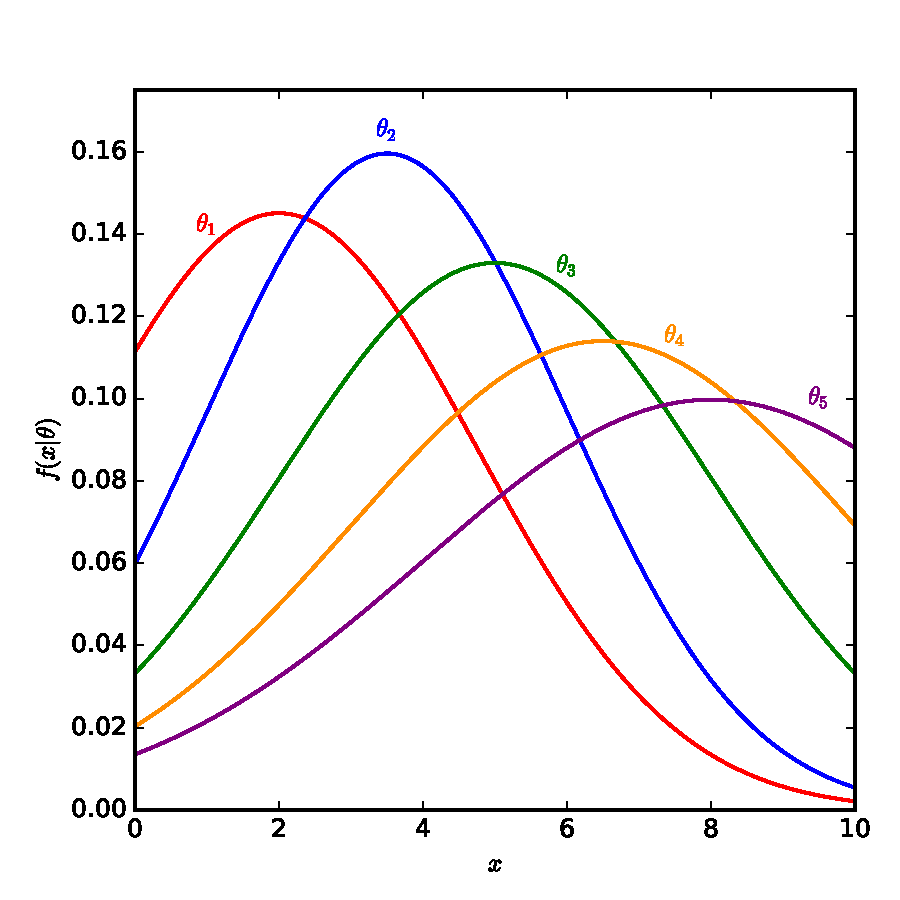
\includegraphics[#1]{fig/general/dummy.pdf}}}

% Math operators
\DeclareMathOperator{\tr}{tr}
\DeclareMathOperator{\Tr}{Tr}
\DeclareMathOperator{\diag}{diag}
\DeclareMathOperator{\Real}{Re}
\DeclareMathOperator{\Pois}{Pois}
\DeclareMathOperator{\cov}{cov}
\DeclareMathOperator{\var}{var}
\DeclareMathOperator{\BR}{BR}
\DeclareMathOperator{\hc}{h.\,c.}

% Title page
\newcommand{\tptitle}[1]{{\sffamily \Huge \bfseries  #1}}
\newcommand{\tpauthor}[1]{{\LARGE #1}}
\newcommand{\tplarge}[1]{{\large #1}}
\newcommand{\tpsmall}[1]{{#1}}
\newcommand{\tpskip}{\vspace{0.18cm}}
\newcommand{\tpbigskip}{\vspace{0.3cm}}

% Capitals at beginning of chapter
\newcommand{\firstword}[2]{\lettrine[lines=3]{\color{highlight-color}#1}{#2}}

% feynmf
\newcommand{\feynmansetup}{%
      \fmfpen{0.8pt}%
      \fmfset{arrow_len}{2mm}%
}

% Very specific things for this thesis
\newcommand{\wbfpyramid}[3]{%
\begin{figure}
%trimming options: L B R T
  \includegraphicsdummy[height=0.225 \textwidth,clip=true,trim=0 1.9cm 2.48cm 0]{fig/information/#1_fw_fb.pdf}\,%
  \phantom{\includegraphicsdummy[height=0.225 \textwidth,clip=true,trim=1.9cm 1.9cm 2.48cm 0]{fig/information/#1_fww_fw.pdf}}\,%
  \phantom{\includegraphicsdummy[height=0.225 \textwidth,clip=true,trim=1.9cm 1.9cm 2.48cm 0]{fig/information/#1_fww_fw.pdf}}\,%
  \phantom{\includegraphicsdummy[height=0.225 \textwidth,clip=true,trim=1.9cm 1.9cm 0 0]{fig/information/#1_fww_fw.pdf}}\\%
%
  \includegraphicsdummy[height=0.225 \textwidth,clip=true,trim=0 1.9cm 2.48cm 0]{fig/information/#1_fbb_fb.pdf}\,%
  \includegraphicsdummy[height=0.225 \textwidth,clip=true,trim=1.9cm 1.9cm 2.48cm 0]{fig/information/#1_fbb_fw.pdf}\,%
  \phantom{\includegraphicsdummy[height=0.225 \textwidth,clip=true,trim=1.9cm 1.9cm 2.48cm 0]{fig/information/#1_fww_fw.pdf}}\,%
  \phantom{\includegraphicsdummy[height=0.225 \textwidth,clip=true,trim=1.9cm 1.9cm 0 0]{fig/information/#1_fww_fw.pdf}}\\%
%
  \includegraphicsdummy[height=0.225 \textwidth,clip=true,trim=0 1.9cm 2.48cm 0]{fig/information/#1_fww_fb.pdf}\,%
  \includegraphicsdummy[height=0.225 \textwidth,clip=true,trim=1.9cm 1.9cm 2.48cm 0]{fig/information/#1_fww_fw.pdf}\,%
  \includegraphicsdummy[height=0.225 \textwidth,clip=true,trim=1.9cm 1.9cm 2.48cm 0]{fig/information/#1_fww_fbb.pdf}\,%
  \phantom{\includegraphicsdummy[height=0.225 \textwidth,clip=true,trim=1.9cm 1.9cm 0 0]{fig/information/#1_fww_fw.pdf}}\\%
%
  \includegraphicsdummy[height=0.27 \textwidth,clip=true,trim=0 0 2.48cm 0]{fig/information/#1_fphi2_fb.pdf}\,%
  \includegraphicsdummy[height=0.27 \textwidth,clip=true,trim=1.9cm 0 2.48cm 0]{fig/information/#1_fphi2_fw.pdf}\,%
  \includegraphicsdummy[height=0.27 \textwidth,clip=true,trim=1.9cm 0  2.48cm 0]{fig/information/#1_fphi2_fbb.pdf}\,%
  \includegraphicsdummy[height=0.27 \textwidth,clip=true,trim=1.9cm 0  0 0]{fig/information/#1_fphi2_fww.pdf}%
  \caption{#3}
  \label{#2}
\end{figure}
}

\newcommand{\thpyramid}[3]{%
\begin{figure}
%trimming options: L B R T
  \includegraphicsdummy[height=0.3 \textwidth,clip=true,trim=0 1.9cm 2.48cm 0]{fig/information/#1_fww_fw.pdf}\,%
  \phantom{\includegraphicsdummy[height=0.3  \textwidth,clip=true,trim=1.9cm 1.9cm 2.48cm 0]{fig/information/#1_fww_fw.pdf}}\,%
  \phantom{\includegraphicsdummy[height=0.3  \textwidth,clip=true,trim=1.9cm 1.9cm 0 0]{fig/information/#1_fww_fw.pdf}}\\%
%
  \includegraphicsdummy[height=0.3 \textwidth,clip=true,trim=0 1.9cm 2.48cm 0]{fig/information/#1_ft_fw.pdf}\,%
  \includegraphicsdummy[height=0.3 \textwidth,clip=true,trim=1.9cm 1.9cm 2.48cm 0]{fig/information/#1_ft_fww.pdf}\,%
  \phantom{\includegraphicsdummy[height=0.3 \textwidth,clip=true,trim=1.9cm 1.9cm 0 0]{fig/information/#1_fww_fw.pdf}}\\%
%
  \includegraphicsdummy[height=0.36 \textwidth,clip=true,trim=0 0 2.48cm 0]{fig/information/#1_fphi2_fw.pdf}\,%
  \includegraphicsdummy[height=0.36 \textwidth,clip=true,trim=1.9cm 0 2.48cm 0]{fig/information/#1_fphi2_fww.pdf}\,%
  \includegraphicsdummy[height=0.36 \textwidth,clip=true,trim=1.9cm 0 0 0]{fig/information/#1_fphi2_ft.pdf}%
  \caption{#3}
  \label{#2}
\end{figure}
}

\title{New Ideas for Effective Higgs Measurements}
\subtitle{PhD Thesis in Progress}
\author{Johann Brehmer}
\date{Version from \today}

\begin{document}

\begin{fmffile}{diagrams}



%%%%%%%%%%%%%%%%%%%%%%%%%%%%%%%%%%%%%%%%%%%%%%%%%%%%%%%%%%%%
%  Front matter
%%%%%%%%%%%%%%%%%%%%%%%%%%%%%%%%%%%%%%%%%%%%%%%%%%%%%%%%%%%%

{
\renewcommand*{\thepage}{cover.\arabic{page}}
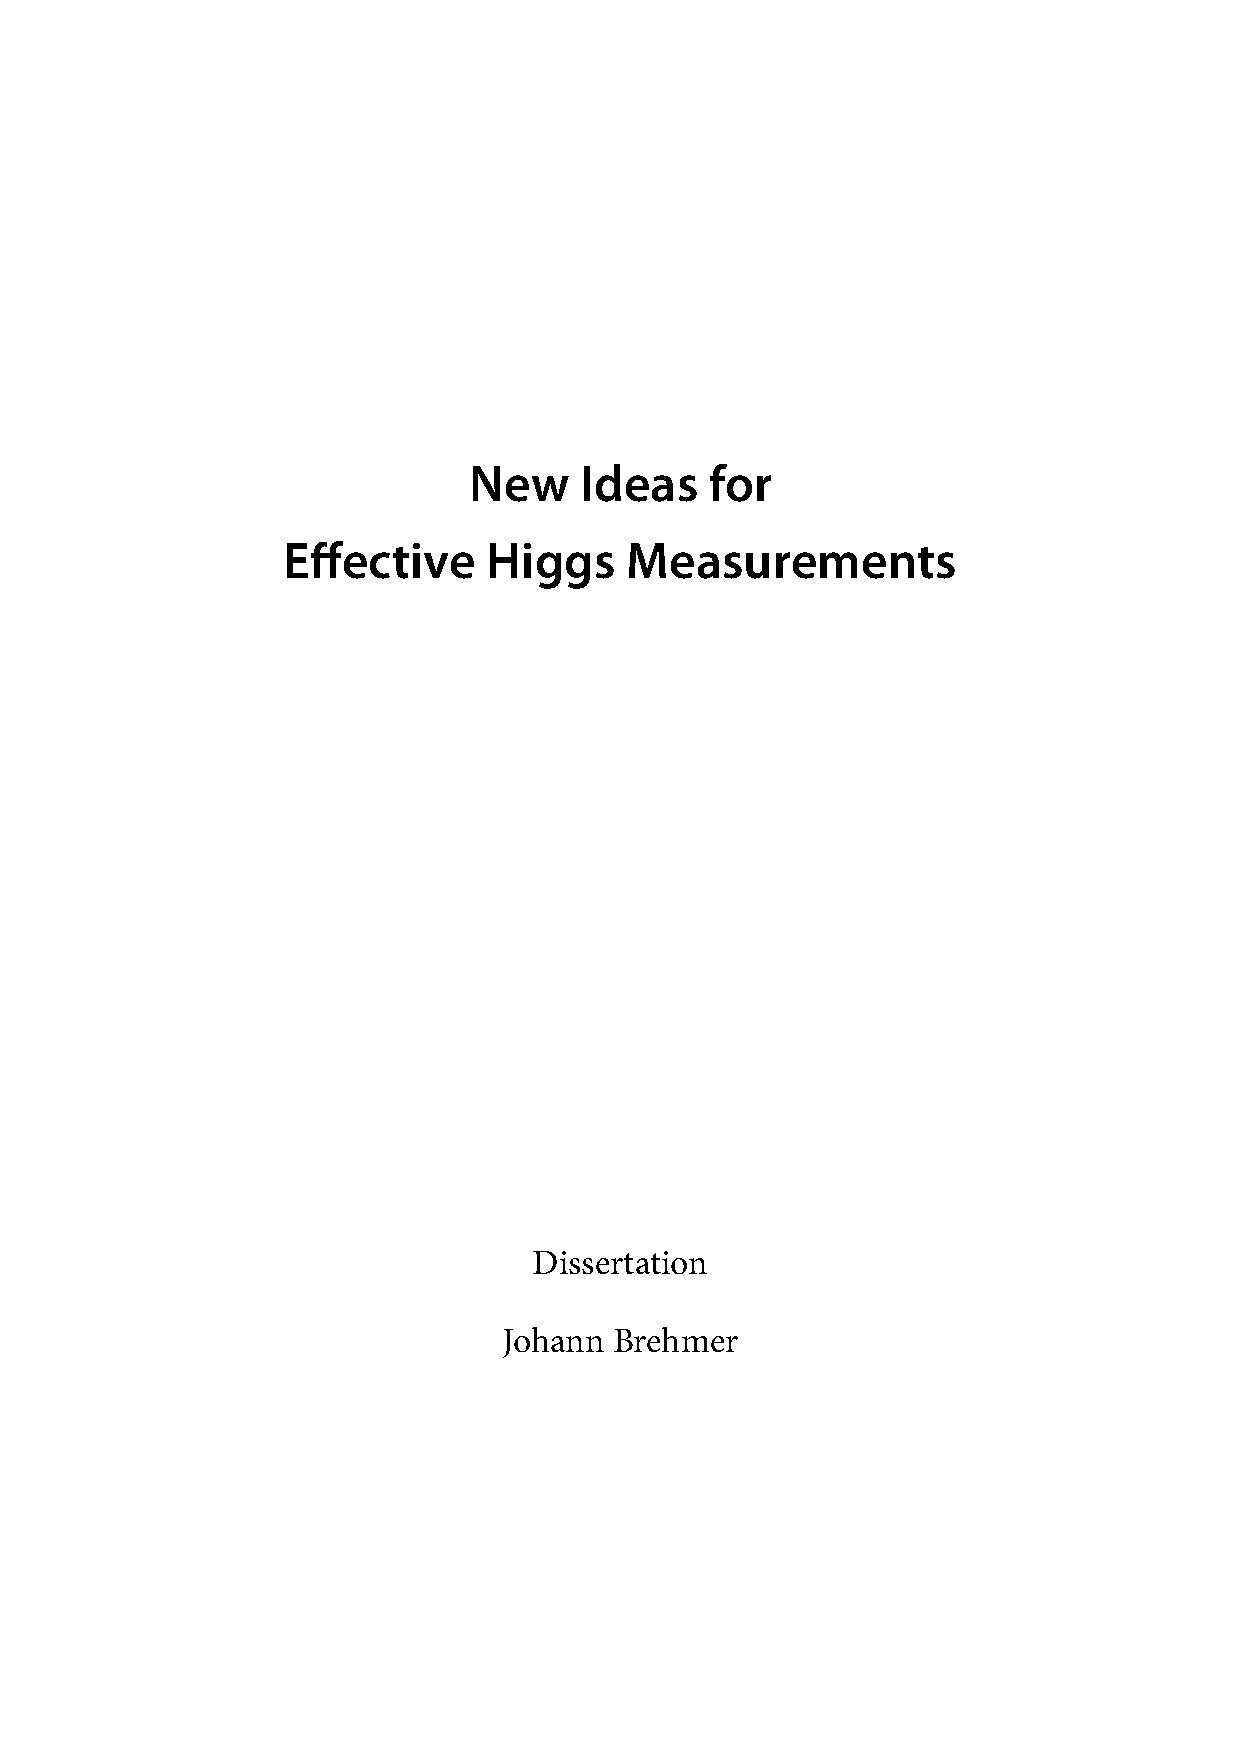
\includepdf{cover/cover.pdf}
\cleardoubleemptypage
}

\frontmatter 
\pagestyle{plain}
\KOMAoptions{cleardoublepage=plain}

% Title and dedication
\begin{titlepage}
  \pagestyle{empty}
  \begin{center}

    % %%%%%%%%%%%%%%%%%%%%%%%%%%%%%%%%%%%%%%%%%%%%%%%%%%%%%%%%%%%%
    % % Repeat cover
    % %%%%%%%%%%%%%%%%%%%%%%%%%%%%%%%%%%%%%%%%%%%%%%%%%%%%%%%%%%%%

    % %\tptitle{On Effective Higgs Measurements}
    % %\tptitle{Efficient Effective Higgs Measurements}
    % %\tptitle{New Ideas for Effective Higgs Measurements}

    % \vspace*{4cm}

    % \tptitle{New Ideas\\[0.7cm]
    %  for Effective Higgs Measurements}

    % % \vspace*{3.5cm}
    % %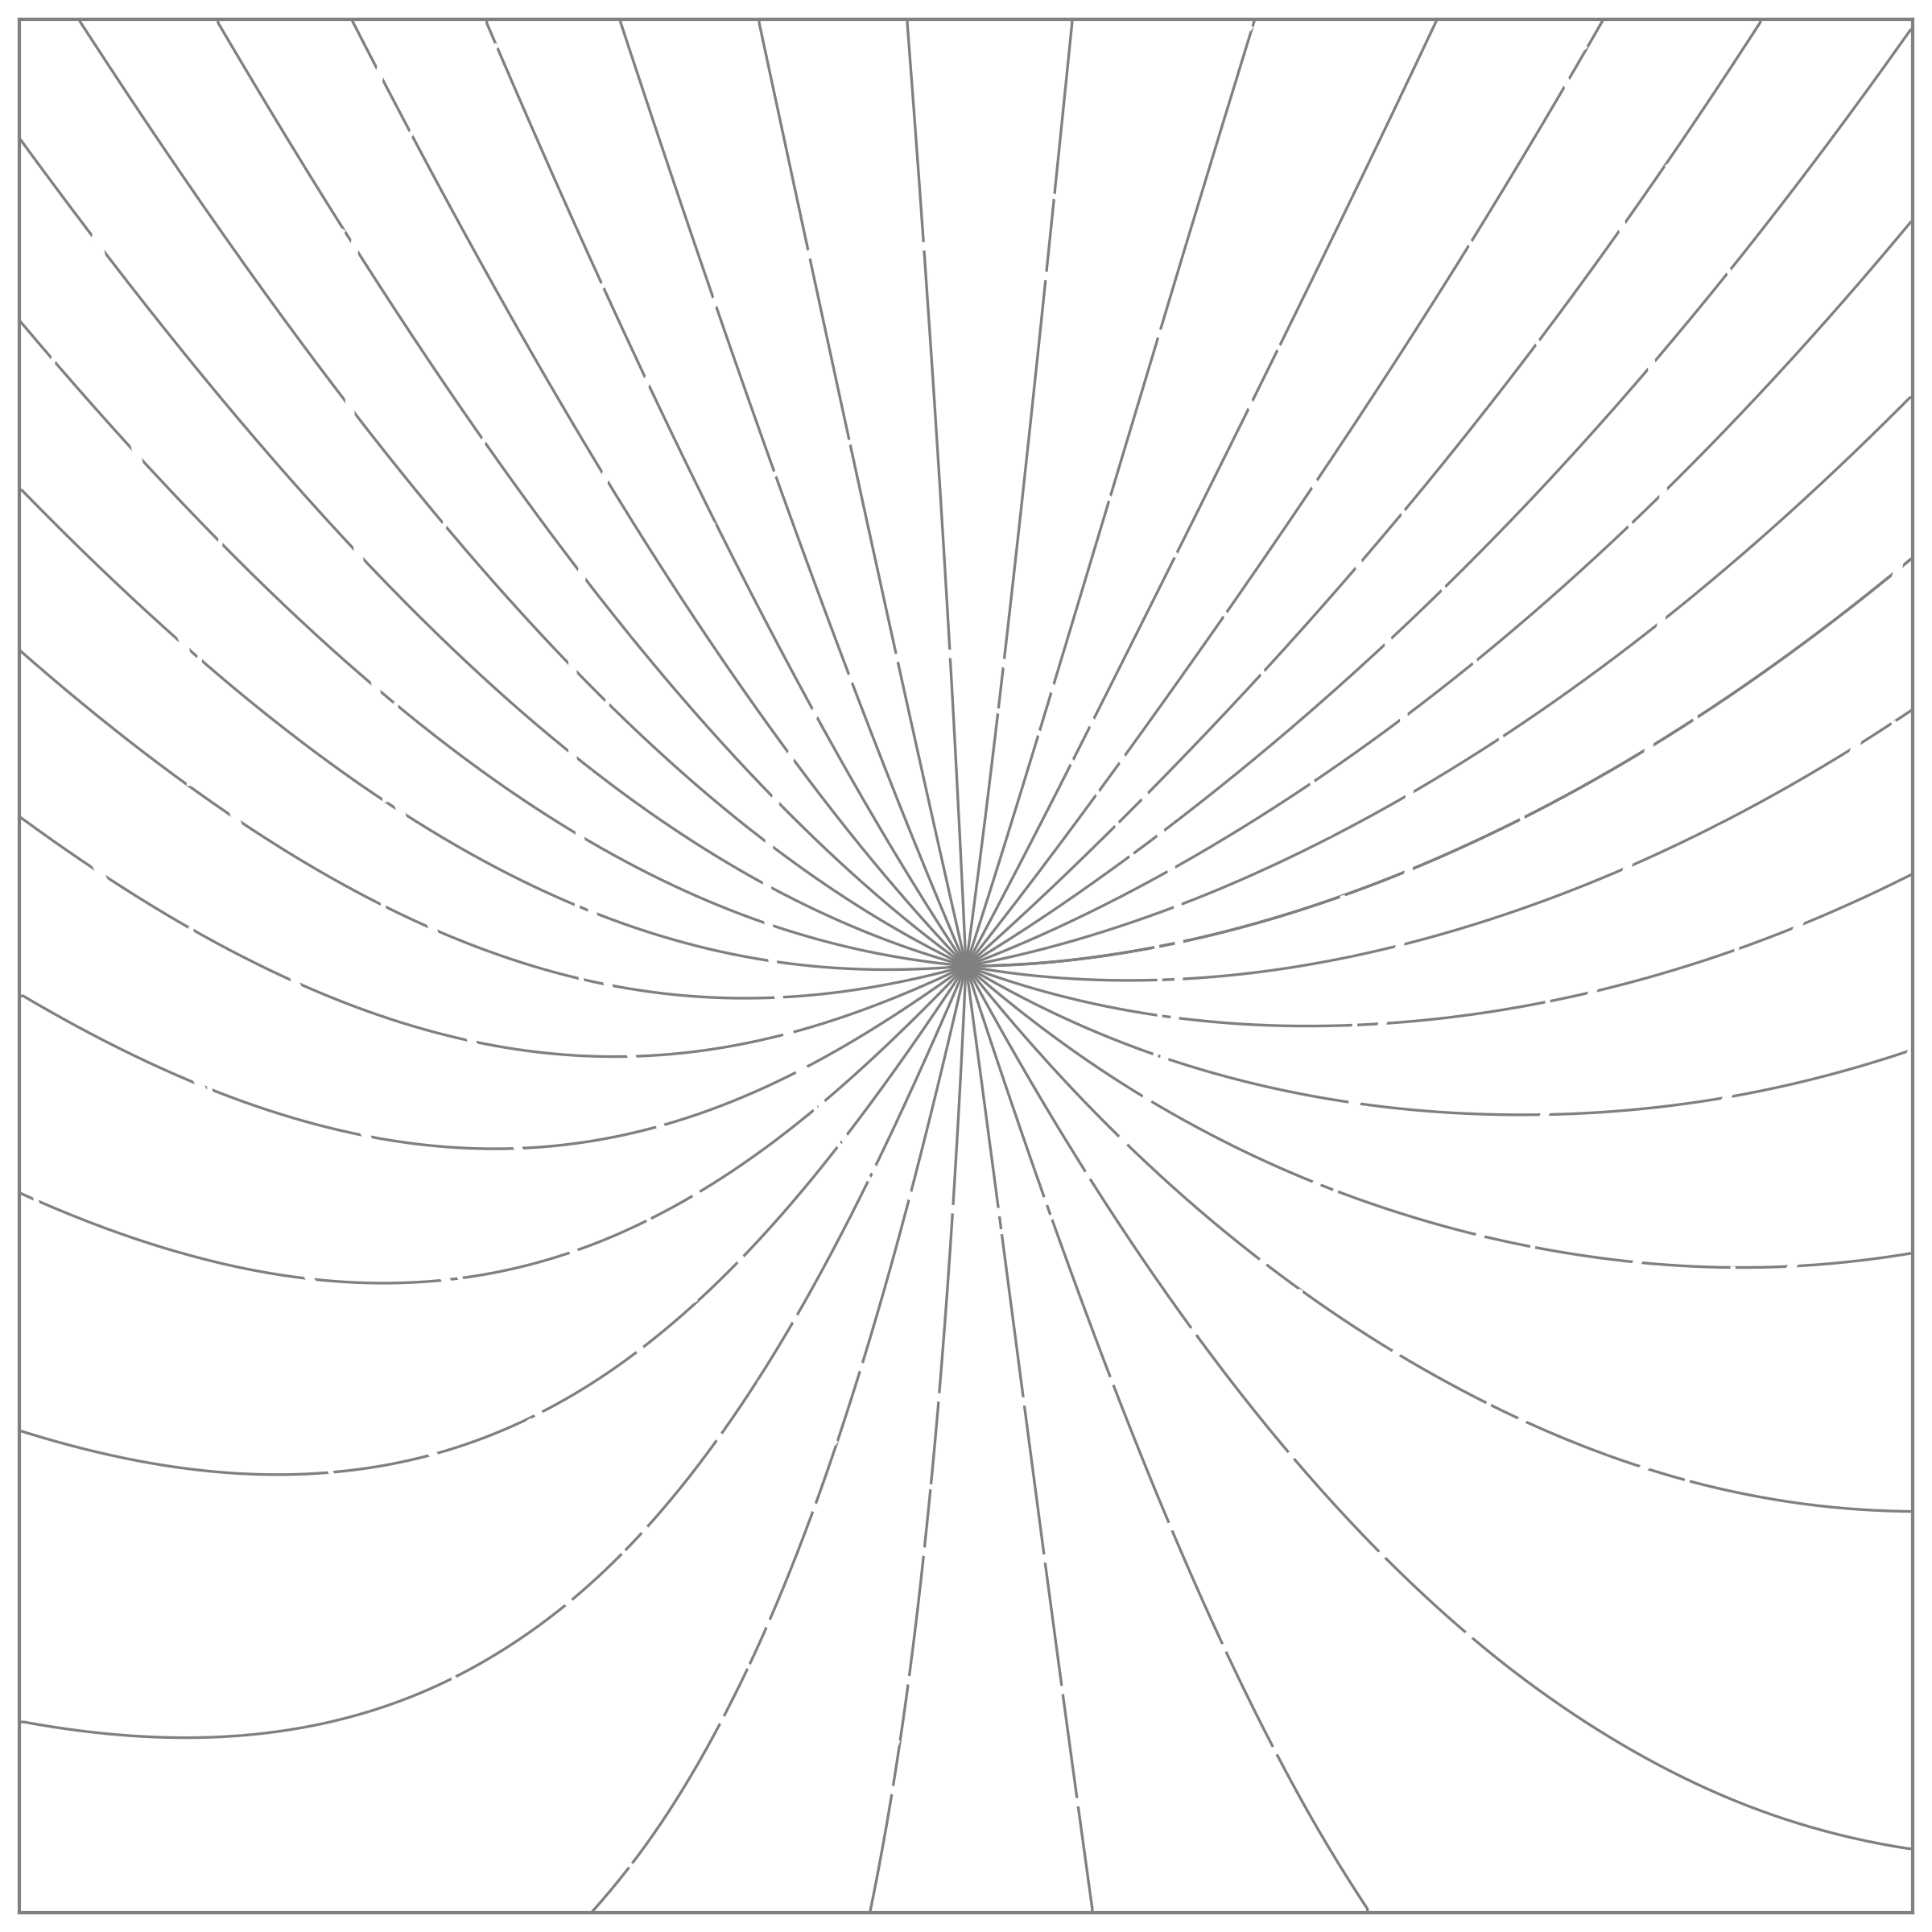
\includegraphics[width=0.6\textwidth]{cover_image.png}
    % %\vspace*{2cm}

    % \vfill

    % \tpauthor{Dissertation\\[0.7cm]
    % Johann Brehmer}

    % \vspace*{2cm}

    % \cleardoubleemptypage 



    %%%%%%%%%%%%%%%%%%%%%%%%%%%%%%%%%%%%%%%%%%%%%%%%%%%%%%%%%%%%
    % First official title page
    %%%%%%%%%%%%%%%%%%%%%%%%%%%%%%%%%%%%%%%%%%%%%%%%%%%%%%%%%%%%

    % \tpauthor{Dissertation}

    % \tpskip

    % \tpsmall{submitted to the Combined Faculties for the Natural Sciences and for Mathematics of the Ruperto-Carola University of Heidelberg, Germany for the degree of Doctor of Natural Sciences}

    \vspace*{2.5cm}



    \tpauthor{Dissertation}

    \tpbigskip

    \tpsmall{submitted to the}

    \tpskip

    \tplarge{Combined Faculties for the Natural Sciences and for Mathematics \\
      of the Ruperto-Carola University of Heidelberg, Germany}

    \tpskip

    \tpsmall{for the degree of}

    \tpskip

    \tplarge{Doctor of Natural Sciences}

    \vfill



    \tpsmall{Put forward by}

    \tpbigskip
 
    \tpauthor{Johann Brehmer}

    \tpbigskip

    \tpsmall{born in Bremen, Germany}

    \vspace*{2cm}



    \tpsmall{Oral examination: July 26, 2017}

    \cleardoubleemptypage 



    %%%%%%%%%%%%%%%%%%%%%%%%%%%%%%%%%%%%%%%%%%%%%%%%%%%%%%%%%%%%
    % Second official title page
    %%%%%%%%%%%%%%%%%%%%%%%%%%%%%%%%%%%%%%%%%%%%%%%%%%%%%%%%%%%%

    \vspace*{3cm}

    \tptitle{New Ideas for\\[0.6cm]
     Effective Higgs Measurements}

  \end{center}

  \vfill

  \noindent \raggedright
  \tabto{0.3 \textwidth} Referees:
  \tabto{0.5 \textwidth} Prof.\ Dr.\ Tilman Plehn \\%
  \tabto{0.5 \textwidth} Prof.\ Dr.\ Bj\"orn Malte Sch\"afer%

\end{titlepage}

\clearpage 

\thispagestyle{plain}

% \widedictum[J.~Cullum~\cite{cullum_twentysomething}]{%
% After years of expensive education\\
% A car full of books and anticipation\\
% I'm an expert on Shakespeare and that's a hell of a lot\\
% But the world don't need scholars as much as I thought
% }

% Abstracts


\selectlanguage{ngerman}
\KOMAoptions{open=left}

%%%%%%%%%%%%%%%%%%%%%%%%%%%%%%%%%%%%%%%%%%%%%%%%%%%%%%%%%%%%
\chapter*{Abstract in deutscher \"{U}bersetzung}
%%%%%%%%%%%%%%%%%%%%%%%%%%%%%%%%%%%%%%%%%%%%%%%%%%%%%%%%%%%%

% Maximum: 200 words 

% Higgs effektive Feldtheorie bietet eine modellunabhängige und
% Phänomenologisch kraftvoller Rahmen für Messungen der Higgs
% Boson Eigenschaften. Wir analysieren zwei Aspekte solcher Messungen
% Für Run ~ 2 des LHC. Erstens kann die begrenzte Präzision des LHC nicht
% Garantieren eine klare Skalenhierarchie zwischen dem experimentellen Momentum
% Transfer und die untersuchte neue Physik Skalen, Zweifel an der
% Gültigkeit des effektiven Modells. Durch den Vergleich einer Reihe neuer Physik
% Szenarien zu ihrer effektiven Approximation, analysieren wir, ob ein
% Beschreibung des Higgs-Sektors mit Dimension-sechs Operatoren ist
% Nützlich, wo die effektive Theorie zerbricht und wie ihre Gültigkeit
% Kann verbessert werden.

% Zweitens verwenden wir Informationsgeometrie, um Higgs zu verstehen und zu optimieren
% Messungen am LHC. Unser neuartiger Ansatz basiert auf dem Fisher
% Informationen, die das maximale Wissen kodieren, auf das man sich beziehen kann
% Parameter in einem gegebenen Experiment. Wir entwickeln einen Algorithmus zu berechnen
% Die Fisher-Information in Teilchenphysikprozessen und berechnen die
% Informationen über Dimension-sechs Operatoren in verschiedenen Higgs-Signaturen.
% Wir zeigen, wie sich Informationsgeometrie ein optimales Ereignis definieren lässt
% Selektionen, bestimmen die mächtigsten kinematischen Observablen und
% Vergleichen die Macht der modernen multivariaten Techniken mit traditionellen
% Histogramm-basierte Analysemethoden.

% \newparagraph
% %

Mit einer effektiven Feldtheorie k\"onnen die Eigenschaften des
Higgs-Bosons ohne starke Theorieannahmen parametrisiert und deren
Messungen effizient kombiniert und interpretiert werden. In dieser
Arbeit untersuchen wir zwei Aspekte, die f\"ur solche Messungen
w\"ahrend Run~2 des LHC relevant sind.

Aufgrund der beschr\"ankten Pr\"azision kann neue Physik im
Higgs-Sektor nur dann entdeckt werden, wenn deren typische
Energieskala nah am experimentellen Impuls\"ubertrag liegt. Die
N\"aherungen der effektiven Theorie sind daher m\"oglicherweise
ung\"ultig. Im ersten Teil dieser Arbeit vergleichen wir die
Signaturen mehrerer Modelle von Physik jenseits des Standardmodells
mit den entsprechenden Beschreibungen in der effektiven Theorie,
untersuchen die N\"utzlichkeit des effektiven Modells, und
demonstrieren, wie dessen G\"ultigkeitsbereich vergr\"o\ss{}ert werden
kann.

Im zweiten Teil verwenden wir Methoden aus der Informationsgeometrie,
um Messungen von Higgs-Eigenschaften zu optimieren. Unser Ansatz
basiert auf der Fisher-Information, die die maximale Pr\"azision
angibt, mit der Parameter in einem Experiment gemessen werden
k\"onnen. Wir entwickeln Methoden zur Berechnung der
Fisher-Information in der Teilchenphysik, und ermitteln die
Information in verschiedenen Higgs-Prozessen. Anschlie\ss{}end zeigen
wir, wie Informationsgeometrie optimale Selektionen und Observablen
definiert und uns das Potential von modernen multivariaten Methoden
mit traditionellen Histogramm-basierten Analysen vergleichen l\"asst.



\selectlanguage{british}
\KOMAoptions{open=right}

%%%%%%%%%%%%%%%%%%%%%%%%%%%%%%%%%%%%%%%%%%%%%%%%%%%%%%%%%%%%
\chapter*{Abstract}
%%%%%%%%%%%%%%%%%%%%%%%%%%%%%%%%%%%%%%%%%%%%%%%%%%%%%%%%%%%%

% Maximum: 200 words

Higgs effective field theory provides a model-independent and
phenomenologically powerful framework to measure the properties of the
Higgs boson. We analyse two aspects of such measurements relevant for
Run~2 of the LHC. First, the limited precision of the LHC cannot
guarantee a clear scale hierarchy between the experimental momentum
transfer and the probed new physics scales, casting doubt on the
validity of the effective model. By comparing a range of new physics
scenarios to their effective approximation, we analyse whether a
description of the Higgs sector with dimension-six operators is
useful, where the effective theory breaks down, and how its validity
can be improved.

Second, we use information geometry to understand and optimise Higgs
measurements at the LHC. Our novel approach is based on the Fisher
information, which encodes the maximum knowledge on theory parameters
one can derive in a given experiment. We develop an algorithm to
calculate the Fisher information in particle physics processes, and
compute the information on dimension-six operators in different Higgs
signatures.  We demonstrate how information geometry lets us define
optimal event selections, determine the most powerful kinematic
observables, and compare the power of modern multivariate techniques
to that of traditional histogram-based analysis methods.


% ToC, LoT, LoF
\microtypesetup{protrusion=false} % disables protrusion for ToC 

%\KOMAoptions{open=left}
\tableofcontents 
%\KOMAoptions{open=right}

\listoffigures
\addcontentsline{toc}{chapter}{List of Figures}

\listoftables 
\addcontentsline{toc}{chapter}{List of Tables}

\microtypesetup{protrusion=true} % enables protrusion again

% Preface and acknowledgements

%%%%%%%%%%%%%%%%%%%%%%%%%%%%%%%%%%%%%%%%%%%%%%%%%%%%%%%%%%%%
\chapter*{Preface}
\label{chapter:preface}
\addcontentsline{toc}{chapter}{Preface}
%%%%%%%%%%%%%%%%%%%%%%%%%%%%%%%%%%%%%%%%%%%%%%%%%%%%%%%%%%%%

This thesis is based on research conducted between 2014 and 2017 at
the Institute for Theoretical Physics at Heidelberg
University. Chapter~\ref{chapter:validity} is based on two articles,
parts of which were incorporated into a CERN report:
% 
\begin{itemize}
  \item[\cite{Brehmer:2015rna}] J.~Brehmer, A.~Freitas, D.~L\'opez-Val, and T.~Plehn:\newline
	\emph{Pushing Higgs Effective Theory to its Limits}.\newline
	Phys.~Rev.~D93 (7), p.~075014, 2016. \arxivlink{1510.03443}.
  \item[\cite{Biekotter:2016ecg}] A.~Biek\"otter, J.~Brehmer, and T.~Plehn:\newline
	\emph{Extending the Limits of Higgs Effective Theory}.\newline
	Phys.~Rev.~D94 (5), p.~055032, 2016. \arxivlink{1602.05202}. 
  \item[\cite{deFlorian:2016spz}] D.~de Florian, C.~Grojean, F.~Maltoni, et al.:\newline
        \emph{Handbook of LHC Higgs Cross Sections: 4.~Deciphering the Nature of the Higgs Sector}.\newline
        LHC Higgs Cross Section Working Group Yellow Report. \arxivlink{1610.07922}.
\end{itemize}
%
Chapter~\ref{chapter:information} is based on the following publication:
%
\begin{itemize}
  \item[\cite{Brehmer:2016nyr}] J.~Brehmer, K.~Cranmer, F.~Kling, and T.~Plehn:\newline
	\emph{Better Higgs Measurements Through Information Geometry}.\newline
       Phys.~Rev.~D95 (7), p.~073002, 2017. \arxivlink{1612.05261}.
\end{itemize}
%
% In addition, it includes some previously unpublished results.
% %
% \begin{itemize}
%   \item[\cite{Brehmer:CPV_information}] J.~Brehmer, F.~Kling, and T.~Plehn:\newline
%     \emph{Understanding CP violation with information geometry} (preliminary title).\newline
%     Work in progress.\comment{Discuss this with Felix and Tilman. Add Tim Tate as author? Title?}
% \end{itemize}
%
Chapter~\ref{chapter:foundations} consists of introductory material
that can be found in textbooks and review articles, and is partly
based on a short lecture I gave to fellow PhD students:
%
\begin{itemize}
  \item[\cite{Brehmer:EFTlecture}]  J.~Brehmer:\newline
	\emph{Higgs Effective Field Theory}.\newline
        Student lecture, research training group `Particle Physics Beyond the Standard Model'.
\end{itemize}

\begin{samepage}
Finally, some of the work done during my PhD is not included in this thesis:
%
\begin{itemize}
  \item[\cite{Brehmer:2015cia}] J.~Brehmer, J.~Hewett, J.~Kopp, T.~Rizzo, and J.~Tattersall:\newline
	\emph{Symmetry Restored in Dibosons at the LHC?} \newline
	JHEP 1510, p.~182, 2015. \arxivlink{1507.00013}.
  \item[\cite{Brehmer:2015dan,Brooijmans:2016vro}] G.~Brooijmans, C.~Delaunay, A.~Delgado, et al.:\newline
         \emph{Les Houches 2015: Physics at TeV Colliders~--~New Physics Working Group Report}.\newline
        \arxivlink{1605.02684}.\newline
         Part of these proceedings were published separately as\newline
         J.~Brehmer, G.~Brooijmans,  G.~Cacciapaglia, et al.:\newline
	\emph{The Diboson Excess: Experimental Situation and Classification of Explanations; A~Les Houches Pre-Proceeding}.\newline
	\arxivlink{1512.04357}.
\end{itemize}
\end{samepage}


%%%%%%%%%%%%%%%%%%%%%%%%%%%%%%%%%%%%%%%%%%%%%%%%%%%%%%%%%%%%
\chapter*{Acknowledgements}
\addcontentsline{toc}{chapter}{Acknowledgements}
%%%%%%%%%%%%%%%%%%%%%%%%%%%%%%%%%%%%%%%%%%%%%%%%%%%%%%%%%%%%

Without doubt, the three years of my PhD were an amazing time. 
% Without doubt, I enjoyed the three years of my PhD tremendously.

For that, I first want to thank my adviser Tilman Plehn: for taking me
on as a student, for working with me on interesting physics, and for
disagreeing with me on countless questions over coffee. But most of
all, I am sincerely grateful to him for always having my back. This
includes him coming into the office on a Sunday morning to get me a
backup laptop when mine broke down days before a deadline.
%
% His support is also, I
% suspect, responsible for the postdoc offers I got.
%
% and, I suspect, some severe
% pulling of strings to make sure I got postdoc offers.
%
% And last but certainly not least, I am grateful to him for clearing
% the way to an academic career for me, even though I finally decided
% against this path.

I would like to thank Bj\"orn Malte Sch\"afer for reading and
refereeing this thesis, and Monica Dunford and Wolfgang Schlegel for
completing my examination committee. Further praise is reserved until
after the defence.

The Research Training Group `Particle physics at the LHC' (DFG GRK
1940) paid my salary and, together with the Heidelberg Graduate School
of Fundamental Physics, my travels. I am grateful for their support.

I had the great pleasure to collaborate with a number of amazing
scientists. Ayres Freitas and David L\'opez-Val saw me off to a great
start and taught me a lot. Anke Biek\"otter joined us a little later,
giving fresh impetus to our research. Chasing the diboson ambulance
with JoAnne Hewett, Joachim Kopp, Tom Rizzo, and Jamie Tattersall was
a wild and fun ride. But one of the best ideas during my PhD was to
grab a beer with Kyle Cranmer in Caf\'e Botanik. Working with him was
inspiring, and was even more fun once Felix Kling joined our team.

The work presented in this thesis benefited greatly from discussions
with others. In particular I would like to express my gratitude to
Anja Butter for keeping me on track with sharp questions, Juan
Gonz\'alez Fraile for teaching me one thing or two about effective
field theories, Torben Schell for being an unwavering source of physics
knowledge as well as a saviour in the hour of incomprehensible linker
errors, and Peter Schichtel for helping me set up and use
\toolfont{MadMax}.

From Marstall lunches to Pheno `class trips', with nut cakes, PhD
hats, and the eternal coffee list, the Heidelberg pheno group was akin
to a second home in the last three years. I would like to thank Martin
Bauer, Anke Biek\"otter, Katja B\"ohnke, Anja Butter, Nishita Desai,
Karin Firnkes, Josua G\"ocking, Juan Gonz\'alez Fraile, Jamil Hetzel,
Sebastian Hoof, Jan Horak, Thomas Hugle, J\"org J\"ackel, Martin
Jankowiak, Florian Jetter, Martin Klassen, Lara Kuhn, Rabea Link,
Viraf Mehta, Luminita Mihaila, Rhea Moutafis, Tilman Plehn, Peter
Reimitz, Michael Russel, Torben Schell, Sebastian Schenk, Peter
Schichtel, Linda Shen, Beatriz Tapia Oregui, Jamie Tattersall,
Valentin Tenorth, Jennifer Thompson, Susanne Westhoff, and Nikolai
Zerf. I am grateful to Anke Biek\"otter, Patrick Foldenauer, and
Sebastian Schenk for the awesome wine\,\&\,cheese seminar. Most of
all, I would like to thank Anja Butter and Torben Schell, who shared
nearly the entire PhD journey with me. Without the two, these three
years would not have been half as much fun.

Further away from the Philosophenweg, I would like to thank the
friends whose company I enjoyed during the last years, and in
particular give a shout out to the Dossenheim gang\,---\,Marcel
Gutsche, Clemens Hassel, and Julia Velte\,---\,and to Christina
Eilers. I want to especially thank Astrid Hiller Blin for
jump-starting many of my days over coffee and arXiv, and for cheering
me on (and up). A big thank you goes to my marvellous parents Antje
and Andreas Brehmer. And then there is Merle Reinhart, who I cannot
thank enough and who in just about any circumstances makes life
better.

If this thesis is legible, it is largely due to the trustworthy proof
readers. I am grateful to Martin Bauer, Anke Biek\"otter, Anja Butter,
Patrick Foldenauer, Juan Gonz\'alez Fraile, Eric Miller, and Sebastian
Schenk. In particular, I am indebted to Astrid Hiller Blin, Antje
Brehmer, and Merle Reinhart, who were crazy enough to read the whole
thing from front to end.

% To all of you, a heartfelt thank you.


\thispagestyle{plain}
\cleardoubleemptypage

%%%%%%%%%%%%%%%%%%%%%%%%%%%%%%%%%%%%%%%%%%%%%%%%%%%%%%%%%%%%
% Higgs theory
%%%%%%%%%%%%%%%%%%%%%%%%%%%%%%%%%%%%%%%%%%%%%%%%%%%%%%%%%%%%


%%%%%%%%%%%%%%%%%%%%%%%%%%%%%%%%%%%%%%%%%%%%%%%%%%%%%%%%%%%%
% Content
%%%%%%%%%%%%%%%%%%%%%%%%%%%%%%%%%%%%%%%%%%%%%%%%%%%%%%%%%%%%

\mainmatter 
\pagestyle{headings}
\KOMAoptions{cleardoublepage=plain}


% \setchapterpreamble[ur]{%
%   \dictum[L.~Carroll~\cite{carroll1898alice}]{%
%     `Begin at the beginning,' the King said, very gravely, `and go
%     on till you come to the end: then stop.' }%
%   \vspace*{2cm}}

%%%%%%%%%%%%%%%%%%%%%%%%%%%%%%%%%%%%%%%%%%%%%%%%%%%%%%%%%%%%
\chapter{Introduction}
\label{chapter:Introduction}
%%%%%%%%%%%%%%%%%%%%%%%%%%%%%%%%%%%%%%%%%%%%%%%%%%%%%%%%%%%%

\firstword{T}{he Higgs boson}~\cite{Higgs:1964ia, Higgs:1964pj,
  Englert:1964et, Guralnik:1964eu, Higgs:1966ev} is the cornerstone
% centrepiece
of the Standard Model of particle physics (SM)~\cite{Glashow:1961tr,
  Weinberg:1967tq, Salam:1968rm}. Its experimental discovery in
2012~\cite{Aad:2012tfa, Chatrchyan:2012xdj}
%
%completed the particle zoo
%of the SM. It
%
% This feat of experimental particle physics
%
is a triumph for a decades-old model, but it also defines a way
forward: the Higgs provides us with an unprecedented chance to
understand some of the biggest unsolved mysteries of physics.

As the only known fundamental scalar, it suffers from the famous
electroweak hierarchy problem: why is its mass scale (and therefore
the electroweak scale) so much smaller than the Planck scale, while
there is no sign of a symmetry protecting it against quantum
corrections? In addition, the Higgs sector is intimately tied to the
stability of the electroweak vacuum and to the unexplained large
hierarchy between the fermion masses. It might also be related to
the open questions of the baryon asymmetry, of the nature of dark
matter, and of inflation.

Many models of physics beyond the Standard Model have been proposed to
explain at least some of these aspects. Often they predict Higgs
coupling patterns different from the SM. A precise measurement of
the Higgs properties thus provides a crucial probe of such models, and
might be one of the most important goals for present and future
runs of the Large Hadron Collider (LHC).

This prospect poses two immediate phenomenological questions:
%
\begin{enumerate}
\item Which framework should be used to parametrise the Higgs
  properties?
\item How can these parameters be measured efficiently at the LHC?
\end{enumerate}
%
% These two topics drive the research presented in this thesis, and we
% will address them one by one.
%
The research presented in this thesis consists of two major parts,
each driven by one of these questions.
%
% These two topics drive the research presented in this thesis, and
% each is addressed in a dedicated chapter.

\newparagraph
%
Regarding the first point, all Higgs measurements should ideally use
the same universal language to parametrise their results, allowing for
an efficient comparison, combination, and interpretation. Such a
framework should be general enough to describe the effects of many
interesting new physics (NP) scenarios without strong model
assumptions.  On the other hand, practical considerations such as
computational resources limit the number of parameters.
%
% On the other hand, too large a number of parameters makes
% statistical analyses and the combinations of different experiments in
% global fits impractical.

A simple example for such a universal parametrisation that was widely
used during Run~1 of the LHC is the $\kappa$ framework. It is based on
the SM Lagrangian, but promotes all Higgs couplings to free
parameters. The main limitation of this approach is that it can only
describe structures that are already present in the SM. While a
measurement based on the $\kappa$ framework can be useful for total
rates, it is not able to utilise information in kinematic
distributions.

Instead, we parametrise new physics signatures with an effective field
theory (EFT)~\cite{Coleman:1969sm, Callan:1969sn,
  Weinberg:1980wa}. Based only on the assumption that new physics has
a typical energy scale significantly larger than the experimental
energies, all new physics effects are captured by a tower of
higher-dimensional operators. The leading effects for Higgs physics
should come from a handful of operators with mass dimension
six~\cite{Burges:1983zg, Leung:1984ni, Buchmuller:1985jz}. These
operators
%
% are manifestly gauge-invariant and can be used beyond tree
% level. They
%
describe both coupling rescalings as well as novel kinematic
structures not present in the SM, allowing us to access information in
distributions in addition to total rates~\cite{Corbett:2012ja,
  Corbett:2015ksa}. Effective operators also let us combine Higgs
measurements with constraints from other processes, including
electroweak precision data or gauge boson production at the
LHC~\cite{Butter:2016cvz}.

However, the limited precision of LHC Higgs measurements is only
sensitive to signatures from models that are either strongly coupled
or relatively light. In the latter case, the characteristic energy
scale of new physics is not clearly separated from the momentum
transfer in the experiments, casting doubt on the validity of the EFT
approach.

We analyse the usefulness of higher-dimensional operators at the LHC
by comparing the predictions of specific scenarios of new physics to
their dimension-six approximations~\cite{Brehmer:2015rna}. Our
analysis covers additional scalar singlets, a two-Higgs-doublet model,
scalar top partners, and heavy vector bosons, focusing on parameter
ranges that the LHC will be sensitive to. We take into account rates
and distributions in the most important Higgs production modes and
representative decay channels as well as in Higgs pair production. For
this array of models, benchmark points, and observables, we ask if and
where the effective description of new physics breaks down, and how it
can be improved.

As it turns out, the performance of the effective model strongly
depends on the matching procedure that links the coefficients of the
dimension-six operators to the full theory. We analyse how electroweak
symmetry breaking affects the validity of the effective theory, and
discuss how the standard matching procedure can be adapted to
situations where these effects are large. In addition, we discuss
whether squared amplitudes from dimension-six operators should be
included in calculations, and which observables provide the best
probes of the momentum transfer in Higgs production in weak boson
fusion~\cite{Biekotter:2016ecg}.

\newparagraph
%
Having chosen a parametrisation of the Higgs properties, the second part
of this thesis focuses on the question of how its parameters can be
measured optimally. Higgs processes are sensitive to many effective
operators. Each of them affects different couplings, typically
introducing non-trivial kinematic structures. This leads to a
complicated relation between the high-dimensional model parameter
space and often also high-dimensional phase spaces.

Conventional analyses based on selection cuts and histograms of
kinematic observables are in many cases not sensitive to such subtle
signatures.  At the other end of the spectrum, experiments resort more
and more to high-level statistical tools, including machine learning
techniques~\cite{Cranmer:2015bka, Louppe:2016ylz, Louppe:2016aov,
  Cranmer:2016lzt, Baldi:2016fzo, Brehmer:ghost_probability,
  Cogan:2014oua, Baldi:2014pta, deOliveira:2015xxd, Almeida:2015jua,
  Baldi:2016fql, Guest:2016iqz, Komiske:2016rsd, Kasieczka:2017nvn,
  Louppe:2017ipp, Baldi:2014kfa, Searcy:2015apa, Santos:2016kno,
  Alves:2016htj, Buckley:2011kc, Bornhauser:2013aya, Bechtle:2017vyu}
or matrix-element-based methods~\cite{Kondo:1988yd, Abazov:2004cs,
  Gao:2010qx, Alwall:2010cq, Avery:2012um, Andersen:2012kn,
  Campbell:2013hz, Artoisenet:2013vfa, Martini:2015fsa,
  Gritsan:2016hjl, Soper:2011cr, Soper:2012pb, Soper:2014rya,
  Atwood:1991ka, Davier:1992nw, Diehl:1993br}. While these
multivariate techniques are powerful, it is often not transparent
which physical properties they probe. It is therefore increasingly
important to be able to characterise the information contained in LHC
signatures.

%We introduce new statistical tools based on information geometry that
%can guide the measurement of continuous theory parameters such as Higgs
%properties~\cite{Brehmer:2016nyr}.
%
We use information geometry~\cite{efron1975, amari1982, amari2000joho}
to understand and optimise the measurement of Higgs properties at the
LHC~\cite{Brehmer:2016nyr}.
%
The central building block of our approach is the Fisher information
matrix, which according to the Cram\'er-Rao bound~\cite{Rao:1945,
  Cramer:1946} encodes the maximal knowledge on theory parameters we
can derive from an experiment. We show that the properties of the
Fisher information make it particularly well-suited to continuous,
high-dimensional parameter spaces, and in particular to effective
field theories.

We develop an algorithm to calculate the Fisher information in
particle physics processes based on Monte-Carlo methods. It allows us
to calculate the maximum precision with which continuous parameters
can be measured in a process. We also analyse how the differential
information is distributed over phase space and how much information
is carried by individual kinematic distributions. This defines the
most powerful phase-space regions and observables for an analysis. It
also allows us to compare how much we can learn from a simple fit to
histograms compared to fully multivariate methods.

These new instruments are then applied to Higgs measurements in three
different channels. We calculate the information on dimension-six
operators in Higgs production in weak boson fusion with decays into
tau pairs and four leptons, and in Higgs production in association
with a single top quark. Finally, we show how our approach can be
extended to include systematic and theory uncertainties, and compare
it to the likelihood ratio.

\newparagraph
%
This thesis begins with a synopsis of essential aspects of Higgs
physics and effective field theories in
\autoref{chapter:foundations}. In \autoref{chapter:validity}, we
discuss the validity of effective field theory for LHC Higgs
measurements and the matching between full models and effective
operators. \autoref{chapter:information} presents our work on
information geometry and efficient measurements of Higgs
properties. Both these chapters contain separate, detailed
introductions and conclusions. We summarise our results in
\autoref{chapter:conclusions}. In a set of appendices we list our
conventions, explain technical details, and provide additional
examples.


% \setchapterpreamble[ur]{%
% \dictum[I.~Berlin~\cite{berlin_blueskies}]{%
% Blue skies smilin' at me\\
% Nothin' but blue skies do I see}%
% \vspace*{2cm}}

\setchapterpreamble[ur]{%
\dictum[G.~R.~R.~Martin~\cite{martin1997game}]{%
``It is known,'' Irri agreed.}%
\vspace*{2cm}}



%%%%%%%%%%%%%%%%%%%%%%%%%%%%%%%%%%%%%%%%%%%%%%%%%%%%%%%%%%%%
\chapter{Foundations}
\label{chapter:foundations}
%%%%%%%%%%%%%%%%%%%%%%%%%%%%%%%%%%%%%%%%%%%%%%%%%%%%%%%%%%%%

\firstword{I}{n this chapter} we review some of the essential concepts
that underlie the research presented in the rest of this thesis. First, we
briefly summarise the role of the Higgs boson in the Standard Model
(SM) and its phenomenology at the LHC.
\autoref{sec:foundations_eft} then presents a pedagogical
introduction to the effective field theory (EFT) concept. In
\autoref{sec:foundations_higgs_eft} we combine these ideas and
introduce Standard Model effective field theory as a universal
language for Higgs physics.

Our introduction to Higgs physics will be superficial, and the EFT
part eschews mathematical rigour for a broad picture of the central
ideas. For a more thorough introduction to Higgs physics, see for
instance Reference~\cite{Plehn:2009nd}. For an extensive introduction to
EFTs, see References~\cite{Georgi:1994qn,Kaplan:2005es}.

The EFT section is based on a lecture given by the author and largely
identical to the lecture notes~\cite{Brehmer:EFTlecture}. Some of the
examples are taken from References~\cite{Georgi:1994qn,Kaplan:2005es}.





%%%%%%%%%%%%%%%%%%%%%%%%%%%%%%%%%%%%%%%%%%%%%%%%%%%%%%%%%%%%
\section{Higgs phenomenology recap}
\label{sec:foundations_Higgs}
%%%%%%%%%%%%%%%%%%%%%%%%%%%%%%%%%%%%%%%%%%%%%%%%%%%%%%%%%%%%


%%%%%%%%%%%%%%%%%%%%%%%%%%%%%%%%%%%%%%%%%%%%%%%%%%%%%%%%%%%%
\subsection{The Standard Model Higgs}
%%%%%%%%%%%%%%%%%%%%%%%%%%%%%%%%%%%%%%%%%%%%%%%%%%%%%%%%%%%%

In the Standard Model, the Higgs field appears as an $SU(2)$ doublet $\phi$ as
%
\begin{multline}
  \lgr{SM} \supset (D^\mu \phi)^\dagger (D_\mu \phi) - \mu^2 \phisq - \lambda (\phisq)^2 \\
            - \sum_{\text{generations}} \left(    y_u {\twovec {\overbar u} {\overbar d}}_L \tilde \phi \, u_{R} 
                                                           + y_d {\twovec {\overbar u} {\overbar d}}_L \phi \, d_{R}
                                                           + y_\ell {\twovec {\overbar \nu} {\overbar \ell^-}}_L \phi \, \ell_{R}   \right )
  \label{eq:foundations_sm_lagrangian}
\end{multline}
%
with
%
\begin{equation}
  D_\mu \phi = \left( \partial_\mu - \im g \frac {\sigma^a} 2 W^a_\mu
    - \im \frac {g'} 2 B_\mu \right) \phi
  \label{eq:foundations_covariant_derivative}
\end{equation}
%
and $\tilde{\phi} = \im \tau_2 \phi^*$. For $\mu^2 < 0$, the Higgs
doublet develops a non-zero vacuum expectation value (VEV)
%
\begin{equation}
  v^2 \equiv 2 \left| \langle {\phi} \rangle \right|^2  = - \frac {\mu^2} \lambda \,.
\end{equation}
%
Using some of the gauge freedom, we can rotate the Higgs field such that
%
\begin{equation}
  \phi = \frac 1 {\sqrt{2}} \twovec  {-w_2 - \im w_1} {v + h + \im w_3} \,,
  \label{eq:foundations_sm_phi}
\end{equation} 
%
where $w_i$ are the would-be Goldstone bosons that give mass to the
$W$ and $Z$ bosons, and $h$ is the physical Higgs boson.

Plugging \autoref{eq:foundations_sm_phi} into
\autoref{eq:foundations_sm_lagrangian}, we find the Higgs mass
%
\begin{equation}
  m_h^2 = {-2\mu^2} = {2\lambda} v^2 \,.
  \label{eq:foundations_higgs_mass_sm}
\end{equation}

The fermions and the massive vector bosons $W^\pm$ and $Z$ get mass
terms proportional to $v$, as well as couplings to the Higgs boson
$h$. Since both terms stem from the same coupling to
$\phi \sim v + h$, the Higgs couplings to other particles are always
proportional to $g_{hxx} \sim m_x / v$. Finally, there are $h^3$ and
$h^4$ self-couplings. The SM Higgs sector is very predictive: With the
measurement of the Higgs mass $m_h = 125~\gev$~\cite{Aad:2012tfa,
  Chatrchyan:2012xdj, Khachatryan:2016vau}, there are no more free
parameters in the SM and all couplings are fixed.



%%%%%%%%%%%%%%%%%%%%%%%%%%%%%%%%%%%%%%%%%%%%%%%%%%%%%%%%%%%%
\subsection{Production and decay channels at the LHC}
%%%%%%%%%%%%%%%%%%%%%%%%%%%%%%%%%%%%%%%%%%%%%%%%%%%%%%%%%%%%

\begin{figure}
  \centering
  \fmfframe(0,15)(15,15){ %(L,T) (R,B)
    \begin{fmfgraph*}(80,60) 
      \feynmansetup
      \fmfleft{i2,i1}
      \fmfright{o1}
      \fmflabel{\small $g$}{i1}
      \fmflabel{\small $g$}{i2}
      \fmflabel{\small $h$}{o1}
      \fmf{gluon}{i1,v1}
      \fmf{gluon}{i2,v2}
      \fmf{fermion,tension=0.1,label=\small $t$,label.side=left}{v1,v2}
      \fmf{fermion,tension=1}{v2,v3,v1}
      \fmf{dashes,tension=3}{v3,o1}
    \end{fmfgraph*}
  }
  \hspace{1cm}
  \fmfframe(0,15)(15,15){ %(L,T) (R,B)
    \begin{fmfgraph*}(100,60)
      \feynmansetup
      \fmfleft{i2,i1}
      \fmfright{o4,o2,o1}
      \fmflabel{\small $q$}{i1}
      \fmflabel{\small $q$}{i2}
      \fmflabel{\small $q$}{o1}
      \fmflabel{\small $h$}{o2}
      \fmflabel{\small $q$}{o4}
      \fmf{fermion,tension=4}{i1,v3}
      \fmf{fermion,tension=4}{i2,v4}
      \fmf{fermion,tension=2.5}{v3,o1}
      \fmf{fermion,tension=2.5}{v4,o4}
      \fmf{wiggly,label=\small $W$,, $Z$,label.side=right}{v3,v5}
      \fmf{wiggly,label=\small $W$,, $Z$,label.side=left}{v4,v5}
      \fmf{dashes,tension=0.5}{v5,o2}
      %\fmfv{decoration.shape=circle,foreground=(0.776,, 0.094,, 0.149),decoration.size=5}{v5}
    \end{fmfgraph*}
  }
  \hspace{1cm}
  \fmfframe(0,15)(15,15){ %(L,T) (R,B)
    \begin{fmfgraph*}(80,60)
      \feynmansetup
      \fmfleft{i2,i1}
      \fmfright{o2,o1}
      \fmflabel{\small $q$}{i1}
      \fmflabel{\small $q$}{i2}
      \fmflabel{\small $h$}{o1}
      \fmflabel{\small $W$, $Z$}{o2}
      \fmf{fermion}{i1,v1,i2}
      \fmf{photon,label=\small $W$,, $Z$}{v1,v2}
      \fmf{dashes}{v2,o1}
      \fmf{photon}{v2,o2}
    \end{fmfgraph*}
  }
  \caption[Feynman diagrams for main Higgs production modes]{Feynman diagrams for
    the most important Higgs production modes considered in this
    thesis. Left: gluon fusion. Middle: weak boson fusion. Right:
    Higgs-strahlung.}
  \label{fig:foundations_production_diag}
\end{figure}

At the LHC, most Higgs bosons are produced in \emph{gluon-gluon
  fusion} as shown in the left panel of
\autoref{fig:foundations_production_diag}. Due to its large Yukawa
coupling, the top plays the dominant role in the loop, with small
contributions from the bottom. The total cross section at
$\sqrt{s} = 13~\tev$ is approximately
$49~\pb$~\cite{deFlorian:2016spz}, a large part of which comes NLO and
NNLO corrections. This sizeable rate comes at the price of a lack of
discerning kinematic features that could help to separate the Higgs
from backgrounds.

This is certainly different for Higgs production in \emph{weak boson
  fusion} (WBF)\footnote{The common name Vector Boson Fusion (VBF)
  forgets that the gluon also has spin 1.}, as shown in the middle
panel of \autoref{fig:foundations_production_diag}. The production
rate for this quark-initiated process is only
$3.8~\pb$~\cite{deFlorian:2016spz}, but the Higgs is accompanied by
two high-energetic jets that point nearly back-to-back in the two
forward regions of the detector. This translates to a large invariant
mass $m_{jj}$ between them as well as a large separation in
(pseudo-)rapidity $\Delta \eta_{jj}$. A second important property is
provided by the colour structure of the process: at leading order,
there is no colour exchange between the two quark lines, which means
there is very little QCD radiation in this process. Both of these
features set the WBF process apart from QCD backgrounds, which
typically have many central jets. Backgrounds can therefore be reduced
significantly by requiring two so-called ``tagging jets'' with large
$\Delta \eta_{jj}$ and large $m_{jj}$, and vetoing any additional
central jets~\cite{Rainwater:1998kj}.

But the tagging jets are not only useful to discriminate Higgs
production from non-Higgs backgrounds. Since they recoil against the
intermediate vector bosons that couple to the Higgs, they provide
access to the momentum flow through the Higgs production vertex. Their
properties, in particular their transverse momenta and the angular
correlations between them, thus provide probes of the Higgs-gauge
coupling. We will revisit this point from different perspectives, and
tagging jet observables will play an important role throughout this
thesis.

The right panel of \autoref{fig:foundations_production_diag}
shows Higgs production in association with a vector boson, or
\emph{Higgs-strahlung}. The rate is $1.4~\pb$ for a $Wh$ final state
plus $0.9~\pb$ for $Zh$. Similarly to the tagging jets in WBF, the
final-state gauge boson both helps to discriminate the Higgs from
backgrounds and provides a handle to access the momentum flow through
the virtual intermediate vector boson. 

\begin{figure}
  \centering
  \fmfframe(0,15)(15,15){ %(L,T) (R,B)
    \begin{fmfgraph*}(120,60)
      \feynmansetup
      %
      \fmfleft{i2,i1}
      \fmfright{o3,o2,o1}
      \fmflabel{\small $q$}{i1}
      \fmflabel{\small $b$}{i2}
      \fmflabel{\small $q$}{o1}
      \fmflabel{\small $h$}{o2}
      \fmflabel{\small $t$}{o3}
      %
      % Upper quark line
      \fmf{fermion,tension=4}{i1,v1}
      \fmf{fermion,tension=2.5}{v1,o1}
      %
      % Lower quark line
      \fmf{fermion,tension=4}{i2,v3}
      \fmf{fermion,tension=2.5}{v3,o3}
      %
      % W exchange 
      \fmf{wiggly,label=\small $W$,label.side=right}{v1,v2}
      \fmf{wiggly,label=\small $W$,label.side=right}{v2,v3}
      %
      % Higgs 
      \fmf{dashes,tension=0.5}{v2,o2}
    \end{fmfgraph*}
  }
  \hspace{1cm}
  \fmfframe(0,15)(15,15){ %(L,T) (R,B)
    \begin{fmfgraph*}(120,60)
      \feynmansetup
      %
      \fmfleft{i2,i1}
      \fmfright{o3,o2,o1}
      \fmflabel{\small $q$}{i1}
      \fmflabel{\small $b$}{i2}
      \fmflabel{\small $q$}{o1}
      \fmflabel{\small $h$}{o2}
      \fmflabel{\small $t$}{o3}
      %
      % Upper quark line
      \fmf{fermion,tension=4}{i1,v1}
      \fmf{fermion,tension=2.5}{v1,o1}
      %
      % Lower quark line
      \fmf{fermion,tension=4}{i2,v2}
      \fmf{fermion,label=\small $t$,label.side=right,tension=5}{v2,v3}
      \fmf{fermion,tension=5}{v3,o3}
      %
      % W exchange 
      \fmf{wiggly,label=\small $W$,label.side=right}{v1,v2}
      %
      % Higgs 
      \fmf{dashes,tension=0.5}{v3,o2}
    \end{fmfgraph*}
  }
  \caption[Feynman diagrams for Higgs plus single top production]{Feynman diagrams for Higgs production with a single top quark.}
  \label{fig:foundations_th_diag}
\end{figure}

We will also briefly analyse \emph{Higgs production with a single top
  quark}. This process exists as an $s$-channel and a $t$-channel
version with very different kinematic features, and can be calculated
either in the four-flavour scheme (with a gluon in the initial state)
or in the five-flavour scheme (with a $b$ quark in the initial
state). We will focus on the dominant $t$-channel process and
calculate it in the five-flavour scheme, as shown in
\autoref{fig:foundations_th_diag}. Diagrams where the Higgs is
radiated off a top quark interfere destructively with amplitudes in
which the Higgs couples to a $W$. The SM rate is small at
$74~\fb$~\cite{deFlorian:2016spz}, but this interference pattern makes
it very sensitive to changes in the top Yukawa coupling. This process
is in fact the only direct probe of the sign or phase of the top
Yukawa coupling ($t \bar{t} h$ production is only sensitive to the
absolute value of the top Yukawa, while the total rate in gluon fusion
can be influenced by many effects such as new particles in the loop).

\begin{figure}[b]
  \centering
  \fmfframe(0,15)(15,15){ %(L,T) (R,B)
    \begin{fmfgraph*}(120,60) 
      \feynmansetup
      \fmfleft{i2,i1}
      \fmfright{o2,o1}
      \fmflabel{\small $g$}{i1}
      \fmflabel{\small $g$}{i2}
      \fmflabel{\small $h$}{o1}
      \fmflabel{\small $h$}{o2}
      \fmf{gluon}{i1,v1}
      \fmf{gluon}{i2,v2}
      \fmf{fermion,tension=0.5,label=\small $t$,label.side=left}{v1,v2}
      \fmf{fermion}{v2,v3}
      \fmf{fermion,tension=0.5}{v3,v4}
      \fmf{fermion}{v4,v1}
      \fmf{dashes}{v3,o2}
      \fmf{dashes}{v4,o1}
    \end{fmfgraph*}
  }
  \hspace{1cm}
  \fmfframe(0,15)(15,15){ %(L,T) (R,B)
    \begin{fmfgraph*}(120,60) 
      \feynmansetup
      \fmfleft{i2,i1}
      \fmfright{o2,o1}
      \fmflabel{\small $g$}{i1}
      \fmflabel{\small $g$}{i2}
      \fmflabel{\small $h$}{o1}
      \fmflabel{\small $h$}{o2}
      \fmf{gluon}{i1,v1}
      \fmf{gluon}{i2,v2}
      \fmf{fermion,tension=0.1,label=\small $t$,label.side=left}{v1,v2}
      \fmf{fermion,tension=1}{v2,v3,v1}
      \fmf{dashes,tension=1.5,label=\small $h$}{v3,v4}
      \fmf{dashes,tension=2}{o2,v4,o1}
    \end{fmfgraph*}
  }
  \caption[Feynman diagrams for Higgs pair production]{Feynman
    diagrams for Higgs pair production.}
  \label{fig:foundations_hh_diag}
\end{figure}

Finally, we will take a look at \emph{Higgs pair production} which
provides a measurement of the Higgs self-coupling~\cite{Plehn:1996wb,
  Baur:2002rb}, see \autoref{fig:foundations_hh_diag}. It is
another example of destructive interference between different
amplitudes: diagrams in which the two Higgses couple to a top box loop
interfere with those in which a single Higgs is produced in gluon
fusion and then splits into two Higgses through the
self-coupling. Close to threshold, these two contributions
approximately cancel in the SM~\cite{Plehn:1996wb, Li:2013rra}, and
the total rate is very small at $33~\fb$. Modified Higgs sectors can
spoil this cancellation and increase the rate drastically.


\newparagraph
%
The Higgs decay patterns are rather simple. Since it couples to all
particles proportional to their mass, it prefers to decay into the
heaviest particles allowed by phase space. The dominant decay mode
with a branching ratio of $58 \%$~\cite{deFlorian:2016spz} are
therefore $b\bar{b}$ pairs. This signature is clearly useless for
Higgs bosons produced in gluon fusion because of the overwhelming QCD
$gg \to b \bar{b}$ background. WBF and $Vh$ production provide handles
to tame these backgrounds, but the channel is still difficult. Easier
to detect are $\tau^+ \tau^-$ pairs with a branching ratio of
$6.3 \%$. Their semi-leptonic and purely leptonic decays involve
neutrinos. But if the taus are boosted enough and not exactly
back-to-back, the neutrino momentum can be reconstructed for instance
using a collinear approximation~\cite{Plehn:2009nd}.

The decays through $W^+W^-$ or $ZZ$ pairs into four-lepton final states
are particularly important due to their clean signatures and because
they provide access to Higgs-gauge couplings. Since the Higgs mass is
below the $W^+W^-$ and $ZZ$  thresholds, one of the vectors has to be
off-shell.\footnote{This also means that branching ratios for
  $h\to ZZ$ and $h \to WW$ are not really well-defined. What is often
  quoted is in fact a term like
  $\br(h \to 4 \ell) / (\br(Z \to \ell^+ \ell^-))^2$.}
$h \to W^+W^- \to (\ell^+ \nu) (\ell^- \overbar{\nu})$ with $\ell = e, \mu$ has a
respectable branching fraction of $1.1 \%$~\cite{deFlorian:2016spz},
but comes with two neutrinos in the final state. Still, it is one of
the most important channels to measure WBF Higgs production. The decay
$h \to ZZ \to 4 \ell$ with $\ell = e, \mu$ provides an extremely
clean signal. Despite its small branching ratio of
$1.3 \cdot 10^{-4}$, it was one of the main Higgs discovery
channels~\cite{Aad:2012tfa,Khachatryan:2016vau}. From a post-discovery
perspective, its four leptons provide a rich spectrum of angular
correlations and other observables that allow us to measure the Higgs
behaviour in detail. We will discuss this feature in more detail
later.

Finally, the small tree-level couplings of the Higgs to light
particles mean that the loop-induced decay into photon pairs can
compete with them. The dominant contribution comes from a $W$ loop,
which interferes destructively with the top loop, resulting in a
branching ratio of $0.23 \%$~\cite{deFlorian:2016spz}. The ATLAS and
CMS detectors are designed to reconstruct photons well, in fact with
exactly this Higgs decay channel in mind. Together with $h \to 4 \ell$
it constitutes the most important channel for the discovery.





%%%%%%%%%%%%%%%%%%%%%%%%%%%%%%%%%%%%%%%%%%%%%%%%%%%%%%%%%%%%
\subsection{How I Learned to Stop Worrying and Love the Higgs}
\label{sec:foundations_relevance}
%%%%%%%%%%%%%%%%%%%%%%%%%%%%%%%%%%%%%%%%%%%%%%%%%%%%%%%%%%%%

There are several facets of the Higgs boson that make it special. From
an experimental point of view, the properties of this shiny new thing
in particle physics are still relatively unknown. Its couplings to
vector bosons and heavy fermions are constrained at the $\ord{10\%}$
level, while for the couplings to light fermions, invisible decays,
and the total decay width of the Higgs there are only weak upper
bounds~\cite{Khachatryan:2016vau, Corbett:2015ksa}. Many of these
limits also rely on specific model assumptions. The top Yukawa
coupling, for instance, is most strongly constrained from the total
Higgs production rate, but only under the assumption that there no new
physics plays a role in the gluon-fusion loop. The total Higgs width
can be constrained indirectly from the contribution of
$g g \to h \to ZZ \to 4 \ell$ in the off-shell Higgs region, but again
relying on strong model assumptions. All in all, the Higgs is still
the least well measured elementary particle (in some sense with the
exception of neutrinos), leaving plenty room for physics beyond the
Standard Model.

\newparagraph
%
From a theory perspective, there are several reasons to suspect
manifestations of new physics in the Higgs sector. Starting with a
rather general argument, the Higgs doublet is the key component of
electroweak symmetry breaking (EWSB), which is often seen as the very
core of the SM construction. A test of the Higgs properties therefore
provides a test of the fundamental structure of Nature.

The Higgs boson is the only fundamental scalar discovered so far. This
is interesting in its own right, but also leads to the famous
electroweak \emph{hierarchy problem}: in the absence of any protective
symmetry, the mass of a scalar field should receive quantum
corrections of the order of the largest scale in the theory. If the SM
is valid all the way to the Planck scale, severe fine-tuning between
the bare parameter and these quantum corrections is necessary to keep
the electroweak mass scale at the observed value. Note that this
argument interchangeably applies to the mass parameter of the Higgs
doublet $\mu^2$, the physical Higgs mass $m_h$, or the electroweak VEV
$v$. Since the strength of the weak force is suppressed by powers of
$m_W \sim v$, and the gravitational force by the Planck scale, the
hierarchy problem is often phrased in terms of the surprising weakness
of gravity compared to the weak force. This naturalness problem is of
a purely aesthetic nature, but similar aesthetic problems have in the
past led to new insights. Many models have been proposed to solve the
hierarchy by introducing a new symmetry that protects the Higgs mass
against quantum corrections.\footnote{An entirely different and
  somewhat metaphysical argument is based on the (weak) anthropic
  principle that observations of the universe are conditional upon its
  laws of physics allowing conscious life~\cite{Weinberg:1987dv,
    Barrow:1988yia}. First, this explanation requires some mechanism
  that generates many different vacua with different values of the
  physics parameters, including the Higgs mass. Most of these vacua
  will have ``natural'' parameters in which the weak and gravitational
  scales are comparable. String theory is hypothesised to provide such
  a sampling mechanism (the ``multiverse''). Second, there has to be a
  reason why larger (and thus more abundant) values of the weak scale
  would not allow any type of intelligent life to form and make
  observations. This question is difficult to answer, and the jury is
  still out~\cite{Agrawal:1997gf, Harnik:2006vj, Clavelli:2006di,
    Giudice:2008bi, Donoghue:2009me, Gedalia:2010iy,
    Adams:2015hvd}. Given the speculative nature of the two questions,
  anthropic reasoning is being criticised as unverifiable or as based
  on arguments from lack of imagination. Some other models such as the
  relaxion~\cite{Graham:2015cka} or
  Nnaturalness~\cite{Arkani-Hamed:2016rle} modify the cosmological
  evolution such that a small Higgs mass is generated dynamically
  during inflation or reheating.}\comment{Citation needed for
  criticism of anthropic principle.} Famous examples are
supersymmetry, composite Higgs models in which the Higgs is the
pseudo-Goldstone boson of some broken symmetry, conformal
symmetries~\cite{Bardeen:1995kv}, or extra dimensions. To reduce
tuning to an acceptable level, this new physics should reside at
energy scales not too far from the electroweak scale. These models
usually modify the Higgs sector in a way that translates into Higgs
couplings different from their SM values.

Another hierarchy unexplained in the SM is the large difference
between the \emph{fermion masses}. There are more than five orders of
magnitude between the top and the electron mass, and neutrinos are
even lighter. Since the fermion masses are generated by the Yukawa
couplings of the Higgs doublet, models that explain the fermion masses
will usually also shift the Higgs-fermion coupling patterns.

The question of \emph{vacuum stability} is still being discussed. The
renormalisation group (RG) allows us to link this question
to the running the quartic coupling $\lambda$ to higher
energies. Current results~\cite{Degrassi:2012ry} indicate that indeed
the quartic coupling becomes negative at large energies, leading to a
second vacuum with lower energy at much larger values of
$\phi$. Fortunately for us, the tunnelling probability is very small,
and in the SM ``our'' vacuum with $v \approx 246~\gev$ seems to be
metastable with a lifetime longer than the age of the universe. While
this indicates there is no pressing need for physics below the Planck
scale to save the electroweak vacuum from a horrible fate, this result
crucially depends on the measured top and Higgs masses, higher-order
corrections to the beta functions, and higher-dimensional operators
stemming from UV physics~\cite{Eichhorn:2015kea}.

In addition to these theoretical and to some degree aesthetic
arguments, there is solid experimental evidence for physics beyond the
SM that might be linked to the Higgs sector. First, the nature of
\emph{dark matter} (DM)~\cite{Plehn:DM} is still unclear. It is experimentally
established that this form of matter is electrically neutral, stable
over cosmological timescales, clumps (i.\,e.\ is now
non-relativistic), and makes up roughly a fourth of the energy density
of the universe. In many models DM is in thermal equilibrium with
ordinary matter in the early universe. Interestingly, the observed
dark matter density is in good agreement with electroweak-scale masses
and weak couplings. This ``WIMP miracle'' is one main reason behind
the popularity of weakly interacting massive particles (WIMPs) as DM
candidates. In this scenario, good candidates for the mediator between
dark matter and the SM are the Higgs boson or other scalars in an
extended Higgs sector. Such ``Higgs portal'' scenarios often predict
signatures in Higgs physics such as modified couplings or invisible
Higgs decays.

Another mystery is the \emph{matter-antimatter asymmetry} of the
universe. Assuming that the cosmos was initially perfectly symmetric,
the observed excess of matter can be generated dynamically if the
three Sakharov conditions are satisfied: there have to be processes
with baryon-number violation as well as $C$ and $CP$ violation, which
take place out of thermal equilibrium. In the SM, these effects are
too small to account for the observed asymmetry. Models that
accommodate larger effects often affect the Higgs sector. In
particular, extended Higgs sectors allow for electroweak symmetry
breaking to be a strong first-order phase transition, providing the
required out-of-equilibrium dynamics. Again, such scenarios predict
signatures in Higgs measurements.

Finally, the Higgs could play another role in the cosmological
evolution of the universe. The origin of the large-scale structure of
the cosmos, the surprising isotropy of the cosmic microwave background
(CMB), and the flatness of the Universe are all explained by an epoch
of exponential expansion of space in the early universe called
\emph{inflation}. This process is often thought to be cause by a
scalar field, the inflaton, slowly rolling down a potential of a
certain shape. In principle the Higgs can be the inflaton, though this
scenario of Higgs inflation requires unnaturally large couplings
between the Higgs and the Ricci scalar, and requires a UV completion.

\newparagraph
%
The null results of the LHC searches for new particles have led to
some disappointment among particle physicists. But with the discovery
of the Higgs boson, the LHC might not only have completed the SM
particle zoo, but rather opened the door to the unknown.  The Higgs
boson is not just another SM particle.  Some of the big open questions
of fundamental physics are deeply rooted in the Higgs sector, and many
other ideas can at least be linked to the Higgs sector under some
assumptions. On the other hand, the current experimental precision
leaves quite some room for signatures of new physics in Higgs
observables. A precise determination of the Higgs properties might be
one of the most exciting measurements at the LHC, and will hopefully
improve our understanding of Nature significantly. Hopefully, the
Higgs boson is not just the last puzzle piece of the Standard Model,
but the first sign of what lies beyond.



%%%%%%%%%%%%%%%%%%%%%%%%%%%%%%%%%%%%%%%%%%%%%%%%%%%%%%%%%%%%
\section{The effective field theory idea}
\label{sec:foundations_eft}
%%%%%%%%%%%%%%%%%%%%%%%%%%%%%%%%%%%%%%%%%%%%%%%%%%%%%%%%%%%%

\comment{Check that all arguments of
  \url{http://indico.cern.ch/event/477407/contributions/2200060/attachments/1369793/2076900/AM_HiggsCouplings2016.pdf}
  are in this section. In particular slide 5.}

This plethora of possible BSM models means that a model-independent
universal theory framework is invaluable for TeV signatures of new
physics. We will consider such a model based on the effective field
theory (EFT) paradigm. Before discussing the specific realisation for
Higgs physics in the next section, here we introduce the general EFT idea.

Effective field theories are a powerful tool that play a role in many,
if not all, areas of physics. Whenever phenomena are spread out over
different energy or length scales, an effective description can be
valuable, either to simplify calculations, or to actually allow
model-independent statements that would be impossible without such a
framework.



%%%%%%%%%%%%%%%%%%%%%%%%%%%%%%%%%%%%%%%%%%%%%%%%%%%%%%%%%%%%
\subsection{Different physics at different scales}
\label{sec:foundations_scales}
%%%%%%%%%%%%%%%%%%%%%%%%%%%%%%%%%%%%%%%%%%%%%%%%%%%%%%%%%%%%

Our world behaves very differently depending on which energy and
length scales we look at. At extremely high energies (or short
distances), Nature might be described by a quantum theory of
gravity. At energies of a few hundred GeV, the Standard Model is
(disappointingly) in agreement with all measurements. Going to lower
energies (or larger distances), we do not have to worry about Higgs or
$W$ bosons anymore: electromagnetic interactions are described by QED,
weak interactions by Fermi theory, strong physics by QCD. Below a GeV,
quarks and gluons are replaced by pions and nucleons as the relevant
degrees of freedom. Then by nuclei, atoms, molecules. At this point
most physicists give up and let chemists (and ultimately biologists
and sociologists) analyse the systems.

The important point here is that the observables at one scale are not
directly sensitive to the physics at significantly different
scales. This is nothing new: for molecules to stick together, the
details of the Higgs sector are not relevant, just as we can calculate how
an apple falls from a tree without knowing about quantum gravity. To
do physics at one scale, we do not have to (and often cannot) take
into account the physics from all other scales. Instead, we isolate
only those features that play a role at the scale of interest.

An effective field theory is a physics model that includes all effects
relevant at a given scale, but not those that only play a role at
significantly different scales. In particular, EFTs ignore spatial
substructures much smaller than the lengths of interest, or effects at
much higher energies than the energy scale of interest.
% In other words, EFTs provide an organized way of approximating
% phenomena that\,---\,at a scale of interest\,---\,are very small as
% zero, and quantities that are very large as infinite.

We will often use examples with one full or underlying theory and
one effective theory. For simplicity, we pretend that the full theory
describes physics correctly at all scales. The EFT is a simpler model
than the full theory and neglects some phenomena (such as heavy
particles) at energy scale $\Lambda$. However, it correctly describes
the physics as long as the observables probe energy scales
%
\begin{equation}
  E \ll \Lambda \,,
  \label{eq:foundations_scale_separation}
\end{equation}
%
within some finite precision. This \emph{scale hierarchy} between the
energy of interest and the scale of high-energy physics not included
in the EFT is the basic requirement for the EFT idea. A validity
range~\eqref{eq:foundations_scale_separation} is a fundamental property of each
EFT.





%%%%%%%%%%%%%%%%%%%%%%%%%%%%%%%%%%%%%%%%%%%%%%%%%%%%%%%%%%%%
\subsubsection{Fermi theory}
%%%%%%%%%%%%%%%%%%%%%%%%%%%%%%%%%%%%%%%%%%%%%%%%%%%%%%%%%%%%

The textbook example for an EFT is Fermi theory, which
describes the charged current interactions between quarks (or
hadrons), leptons and neutrinos at low energies. The underlying model
here is the SM, in which this weak interaction is mediated by the
exchange of virtual $W$ bosons with mass $m_W$ and coupling constant
$g$:
%
\begin{equation}
  \mathcal{M}_\text{full} \sim {}
  \raisebox{-0.5\height}{
    %\fbox{
      \fmfframe(0,10)(0,10){ %(L,T) (R,B)
        \begin{fmfgraph*}(70,40) 
          \feynmansetup
          \fmfleft{i2,i1}
          \fmfright{o2,o1}
          \fmflabel{\small $f_1$}{i1}
          \fmflabel{\small $f_2$}{i2}
          \fmflabel{\small $f_3$}{o1}
          \fmflabel{\small $f_4$}{o2}
          \fmf{fermion}{i1,v1,i2}
          \fmf{fermion}{o1,v2,o2}
          \fmf{boson,tension=1,label=\small $W$}{v1,v2}
          \marrow{m}{up}{top}{$p$}{v1,v2}
          \fmflabel{\small $g$}{v1}
          \fmflabel{\small $g$}{v2}
        \end{fmfgraph*}
      }
    %}
  }
  {} \sim - \frac {g^2} {p^2 - m_W^2}
  \label{eq:foundations_4fermion_full}
\end{equation}
%
In Fermi theory, there are no $W$ bosons, just a direct
interaction between four fermions with coupling constant
$G_F \propto g^2 / m_W^2$:
%
\begin{equation}
  \mathcal{M}_\text{EFT} \sim {}
  \raisebox{-0.5\height}{
    %\fbox{
      \fmfframe(0,10)(0,10){ %(L,T) (R,B)
        \begin{fmfgraph*}(50,40) 
          \feynmansetup
          \fmfleft{i2,i1}
          \fmfright{o2,o1}
          \fmflabel{\small $f_1$}{i1}
          \fmflabel{\small $f_2$}{i2}
          \fmflabel{\small $f_3$}{o1}
          \fmflabel{\small $f_4$}{o2}
          \fmf{fermion}{i1,v,i2}
          \fmf{fermion}{o1,v,o2}
          \fmflabel{\small $G_F$}{v}
          \fmfv{decor.shape=circle,decor.filled=full, decor.size=5}{v}
        \end{fmfgraph*}
      }
    %}
  }
  {} \sim G_F \propto \frac {g^2} {m_W^2}
  \label{eq:foundations_4fermion_EFT}
\end{equation}
%
So the EFT turns the $W$ propagator into a contact interaction between
the fermions, shrinking the distance bridged by the virtual $W$ to
zero. Clearly, the two amplitudes agree as long as the momentum
transfer through the vertex is small,
$E^2 = p^2 \ll \Lambda^2 = m_W^2$:
%
\begin{equation}
  - \frac {g^2} {p^2 - m_W^2}
  = \frac {g^2} {m_W^2} \left(1 +  \frac {p^2} {m_W^2} + \ord{p^4/m_W^4} \right)
  \approx  \frac {g^2} {m_W^2} \,.
\end{equation}

One process described by this interaction is muon decay. Its typical
energy scale $E \approx m_\mu$ is well separated from $\Lambda = m_W$,
and Fermi theory will describe the process quite accurately. The
relative \emph{EFT error}, i.\,e.\ the mistake we make when
calculating an observable with the EFT rather than with the full
model, should be of order $\Delta_\text{EFT} = \Gamma_\text{EFT} / \Gamma_\text{full}  \sim E^2 / \Lambda^2 \sim m_\mu^2 / m_W^2 \approx 10^{-6}$.

In proton collisions at the LHC the same interaction takes place, but
at potentially much larger momentum transfer $E < 13$~TeV. The EFT
error increases with $E$. For $E \gtrsim m_W$, the full model allows
on-shell $W$ production, a feature entirely missing in the EFT. Here
the two descriptions obviously diverge and Fermi theory is no longer a
valid approximation of the weak interaction.



%%%%%%%%%%%%%%%%%%%%%%%%%%%%%%%%%%%%%%%%%%%%%%%%%%%%%%%%%%%%
\subsubsection{Down and up the theory ladder}
%%%%%%%%%%%%%%%%%%%%%%%%%%%%%%%%%%%%%%%%%%%%%%%%%%%%%%%%%%%%

In reality there are of course more than two theories, and the notion
of underlying and effective model becomes relative. The SM itself is
not valid up to arbitrary large energies: it does not explain dark
matter, the matter-antimatter asymmetry, or gravity. It is probably
also internally inconsistent since at some very large energy the
quartic coupling $\lambda$ and the coupling constant $g'$ hit Landau
poles. So the SM is an effective theory with validity range
$E \ll \Lambda \le M_{Pl}$ and has to be replaced by some other
description at larger energies. On the other hand, going to energies
lower than a few GeV, the relevant physics changes again and we should
switch to a new effective theory. In this way, all theories can be
thought of as a series of EFTs, where the model valid at one scale is
the underlying model for the effective theory at the next lower scale.

If you think you know a theory that describes our world at
sufficiently large energies, then in principle there is no need to use
effective theories: you can calculate every single observable in your
full model (at least if the full model is perturbative at these
energies or other approximations such as lattice calculations are
available). This will however make hard calculations necessary even
for the simplest low-energy processes. One can save a lot of
computational effort and focus on the relevant physics by dividing the
phase space into regions with different appropriate effective
descriptions.

Starting from a high energy scale where the parameters of the
fundamental theory are defined, these parameters are run to lower
energies until the physics changes substantially. At this
\emph{matching scale} an effective theory is constructed from the full
model, and its coefficients are determined from, or matched to, the
underlying model. Then the coefficients of this EFT are run down to
the next matching scale, where a new EFT is defined and its parameters
are calculated, and so on. This is the \emph{top-down} view of
EFTs. For instance, we can start from the SM and construct Fermi
theory as a simpler model valid at low energies. While we can
certainly use the SM to calculate the muon lifetime, it is not
necessary, and a calculation in Fermi theory is quite accurate and
simpler.

But often we do not know the underlying theory. As mentioned above,
there has to be physics beyond the SM, and there is still hope it will
appear around a few TeV. If we want to parametrise the effects of such
new physics on electroweak-scale observables, we do not know how the
full model looks like. But even without knowing the underlying model,
we can still construct an effective field theory based on a few very
general assumptions. We will go through these ingredients in the next
section. For this \emph{bottom-up} approach, an effective theory is
not only useful, but actually the only way we can discuss new physics
without choosing a particular model of BSM physics.

High-energy physics can be seen as the field of working ourselves up a
chain of EFTs to ever higher energies. But how does this chain end?
Does it end at all? Even if we one day find a consistent theory that
can explain all observations to date, how would we check if it indeed
describes Nature up to arbitrarily high energies? Understanding all
theories as effective, these questions do not matter! The EFT
framework provides us with the tools to do physics without having to
worry about the far ultraviolet.

% To summarize this introduction, the basic EFT idea is to take into
% account only the phenomena relevant at the scale of interest. With
% this broad definition one can even say that effective theories are
% pretty much the only way we can do physics at all. The question is
% not \emph{if} one should use an EFT for a given process (after all,
% what would be the alternative?), but \emph{which} effective theory
% is the best one for a given process, especially in light of the
% validity range of all effective theories.

% There is nothing strange or complicated about effective field
% theories. They simply provide an organized way of doing what we always
% do in physics: neglecting effects that do not matter for a given
% question. EFTs in the form of quantum field theories consist of a set
% of (typically non-renormalizable) operators. You have seen how this
% framework allows us to start with a full theory and constructive an
% effective approximation from the top down, and how it even allows us
% to construct an approximate description of physics even if we do not
% know the underlying theory.



%%%%%%%%%%%%%%%%%%%%%%%%%%%%%%%%%%%%%%%%%%%%%%%%%%%%%%%%%%%%
\subsection{EFT construction and the bottom-up approach}
\label{sec:foundations_eft_bottom_up}
%%%%%%%%%%%%%%%%%%%%%%%%%%%%%%%%%%%%%%%%%%%%%%%%%%%%%%%%%%%%

EFTs are especially useful in the framework of quantum field theory
(QFT). Before showing how to construct the effective operators of such
a theory in a bottom-up approach, let us recapitulate how QFTs are
organised.



%%%%%%%%%%%%%%%%%%%%%%%%%%%%%%%%%%%%%%%%%%%%%%%%%%%%%%%%%%%%
\subsubsection{Reminder: operators and power counting}
%%%%%%%%%%%%%%%%%%%%%%%%%%%%%%%%%%%%%%%%%%%%%%%%%%%%%%%%%%%%

The basic object describing perturbative QFTs in $d=4$ flat space-time
dimensions is the action
%
\begin{equation}
  S = \intfourx \lgr{}(x) \,.
  \label{eq:foundations_action}
\end{equation}
%
The Lagrangian $\lgr{}(x)$ is a sum of couplings times operators,
where the operators are combinations of fields and derivatives
evaluated at one point $x$. These are either kinematic terms, mass
terms or represent interactions between three or more fields. For
instance, the Lagrangian
%
\begin{equation}
  \lgr{} =  \im  \bar{\psi}_i \gamma^\mu \partial_\mu \psi_i - \frac 1 4 V_{\mu \nu} V^{\mu \nu} 
  - m_i \bar{\psi}_i \psi_i + m_V^2 V_\mu V^\mu
  - g \bar{\psi}_i \gamma_\mu \psi_i V^\mu
  \label{eq:foundations_action_V_fermions}
\end{equation}
%
with implicit sum over $i$ describes fermions $\psi_i$, a massive
vector boson $V_\mu$, and an interaction between them with coupling
$g$.\footnote{Massive vector bosons have issues with renormalisability
  and unitarity, which can be solved by generating the mass in a Higgs
  mechanism at a higher scale, but this irrelevant for the discussion
  here.}

A key property of each coupling or operator is its \emph{canonical
  dimension} or mass dimension. In simple terms this can be formulated
as the following question: if you assign a value to a quantity, which
power of a mass unit such as GeV would this value carry? Since we work
in units with $\hbar = c = 1$, length and distance dimensions are just
the inverse of mass dimensions. We will denote the mass dimension of
any object with squared brackets, where $[\ope{}] = D$ means that
$\ope{}$ is of dimension mass$^D$, or mass dimension $D$.

In QFT, the action can appear in exponentials such as $e^{\im S}$, so
it must be dimensionless: $[S] = 0$. The space-time integral in
\autoref{eq:foundations_action} then implies $[\lgr{}] = d = 4$, so every term
in the Lagrangian has to be of mass dimension 4. Applying this to the
kinetic terms, we can calculate the mass dimension of all fields. This
then allows us to calculate the mass dimension or canonical dimension of operators and
couplings in the theory.

In the example in \autoref{eq:foundations_action_V_fermions}, the kinetic term
for the fermions contains one space-time derivative, $[\partial] =
1$.
To get $[\bar{\psi} \partial \psi] = 4$, the fermion fields must have
dimension $[\psi_i] = 3/2$. Similarly, the field strength $V_{\mu\nu}$
contains a derivative, so we end up with $[V_\mu] = 1$. With these
numbers we can check the other operators. In addition to the expected
$[m] = [m_V] = 1$, we find $[\bar{\psi} \psi V^\mu] = 4$ or $[g] = 0$.

The canonical dimension of an operator has two important
consequences. First, the renormalisation group flow of a theory,
i.\,e.\ the running of the couplings between different energy scales,
largely depends on the mass dimensions of the operators. Operators
with mass dimension $D < d$ (``relevant'' operators) receive large
quantum corrections when going from large energies to low energies.
This is a key argument for many fine-tuning problems such as the
hierarchy problem or the cosmological constant problem. On the other
hand, operators with $D > d$ (``irrelevant'' ones) are typically
suppressed when going to lower energies. Operators with $D = d$ are
called ``marginal''.

The second consequence of the mass dimension affects the
renormalisability of a theory. Theories with operators with $D > d$
are \emph{non-renormalisable}:\footnote{The opposite is not true: some
  theories contain only operators with $D \le d$, but are still not
  renormalisable.} particles in loops with energies $E \to \infty$
will lead to infinities in observables, and they are too many to be
hidden in a renormalisation of the parameters.



%%%%%%%%%%%%%%%%%%%%%%%%%%%%%%%%%%%%%%%%%%%%%%%%%%%%%%%%%%%%
\subsubsection{Effective operators}
%%%%%%%%%%%%%%%%%%%%%%%%%%%%%%%%%%%%%%%%%%%%%%%%%%%%%%%%%%%%

From now on we will only consider EFTs realised as a local QFT in 4
space-time dimensions, an approach that has proven very successful in
high-energy physics so far. EFTs are then defined as a sum of
operators $\ope{i}$, each with a specific canonical dimension $D_i$. We can
split the coupling in front of each operator into a dimensionless
constant, the \emph{Wilson coefficient} $f_i$, and some powers of a
mass scale, for which we use the scale of heavy physics $\Lambda$:
%
\begin{equation}
  \lgr{EFT} = (\text{kinetic and mass terms}) + \sum_i \frac {f_i} {\Lambda^{D_i - d}} \, \ope{i} \,.
  \label{eq:foundations_EFT_lagrangian}
\end{equation}
%
Why do we force $\Lambda$ to appear in front of the operators like
this? If we do not know anything about the underlying model at scale
$\Lambda$, our best guess (which can be motivated with arguments based
on the renormalisation group flow) is that it consists of
dimensionless couplings $g \sim \ord{1}$ and mass scales
$M \sim \ord{\Lambda}$. Indirect effects mediated by this high-energy
physics should therefore be proportional to a combination of these
factors, as given in \autoref{eq:foundations_EFT_lagrangian} with
couplings $f_i \sim \ord{1}$. This is certainly true in Fermi theory,
where the effective coupling $G_F$ is suppressed by
$\Lambda^2 = m_W^2$.


  
% %%%%%%%%%%%%%%%%%%%%%%%%%%%%%%%%%%%%%%%%%%%%%%%%%%%%%%%%%%%%
% \subsubsection{Full and effective descriptions of physics}
% %%%%%%%%%%%%%%%%%%%%%%%%%%%%%%%%%%%%%%%%%%%%%%%%%%%%%%%%%%%%

% Let us go back to the simple picture of one full and one effective
% theory and summarise the typical differences between the two setups.
% %
% \begin{itemize}
% \item The full model contains high-energy physics, for instance heavy
%   particles with mass $\gtrsim \Lambda$ that are not dynamical degrees
%   of freedom in the EFT. In the effective model their effects are
%   mapped onto additional higher-dimensional operators involving only
%   the light fields.
% %
% \item At least in our simple picture we assume that the full model is
%   valid at all energies. The EFT, in any case, is only valid at
%   $E \ll \Lambda$. Only in this low-energy region the two descriptions
%   agree, at $E \gtrsim \Lambda$ the EFT predictions will not reproduce
%   the full model.
% %
% \item The full model is fully renormalisable, while the EFT is
%   typically only renormalisable order by order.
% %
% \item An interaction mediated by heavy fields in the full model is
%   described by the higher-dimensional operators in the EFT, see for
%   instance Esq.~\eqref{eq:foundations_4fermion_full} and
%   \eqref{eq:foundations_4fermion_EFT}. This means that the non-local
%   interaction in the full model is approximated as a local contact
%   interaction in the EFT.
% \end{itemize}



%%%%%%%%%%%%%%%%%%%%%%%%%%%%%%%%%%%%%%%%%%%%%%%%%%%%%%%%%%%%
\subsubsection{Ingredients}
%%%%%%%%%%%%%%%%%%%%%%%%%%%%%%%%%%%%%%%%%%%%%%%%%%%%%%%%%%%%

How the operators $\ope{i}$ look like might be clear in a top-down
situation where we know the underlying theory. In a bottom-up
approach, however, we need a recipe to construct a list of operators
in a model-independent way. It turns out that this is surprisingly
straightforward, and the list of operators we need to include in the
EFT is defined by three ingredients: the particle content, the
symmetries, and a counting scheme that decides which operators are
relevant at the scale of interest. We will go through them one by one.

\begin{enumerate}
\item \emph{Particle content}: one has to define the fields that are
  the dynamical degrees of freedoms in the EFT, i.\,e.\ that can form
  either external legs or internal propagators in Feynman diagrams. At
  least all particles with masses $m \ll \Lambda$ should be
  included. The operators are then combinations of these fields and
  derivatives.
%
\item \emph{Symmetries}: some symmetry properties of the world have
  been measured with high precision, and we can expect that a
  violation of these symmetries has to be extremely small or happens
  at very high energies. These can be gauge symmetries (such as the
  $SU(3) \times SU(2) \times U(1)$ of the SM), space-time symmetries
  (such as Lorentz symmetry), or other global symmetries (such as
  flavour symmetries). Requiring that the effective operators do not
  violate these symmetries is well motivated and can reduce the
  complexity of the theory significantly.
%
\item \emph{Counting scheme}: with a set of particles and some
  symmetry requirements we can construct an infinite tower of
  different operators. We therefore need some rule to decide which of
  the operators we can neglect. Here the dimensionality of the
  operators becomes important. As argued above, we expect an operator
  with canonical dimension $D > d$ to be suppressed by a factor of roughly
  $1 / \Lambda^{D-d}$. Operators of higher mass dimension are
  therefore more strongly suppressed. Setting a maximal operator
  dimension is thus a way of limiting the EFT to a finite number of
  operators that should include the leading effects at energies
  $E \ll \Lambda$.
\end{enumerate}

One property that is often required of theories is missing in this
list: an EFT (with its intrinsic UV cutoff $\Lambda$) does not have to
be renormalisable in the traditional sense. In fact, most EFTs include
operators with mass dimension $D > d$ and are thus non-renormalisable.
However, EFTs are still renormalisable order by order in the counting
scheme, and loop effects can be calculated without any fundamental
issues. 



%%%%%%%%%%%%%%%%%%%%%%%%%%%%%%%%%%%%%%%%%%%%%%%%%%%%%%%%%%%%
\subsubsection{Basis choices}
%%%%%%%%%%%%%%%%%%%%%%%%%%%%%%%%%%%%%%%%%%%%%%%%%%%%%%%%%%%%

Usually not all operators that can be constructed in this way are
independent. This can be seen from a field redefinition of the form
%
\begin{equation}
  \phi(x) \to \phi'(x) = \phi(x) + \varepsilon f(x)
\end{equation}
%
where $\varepsilon$ is some small parameter and $f(x)$ can contain any
combination of fields evaluated at $x$. The action in terms of the new
field is then (after integration by parts)
%
\begin{equation}
  \intfourx \lgr{}[\phi] \to \intfourx \lgr{}[\phi']
  % &= \intfourx \left( \lgr{}[\phi] + \varepsilon \fder {\lgr{}} {\phi} f + \varepsilon \fder {\lgr{}} {\partial_\mu \phi} \partial_\mu f + \ord{\varepsilon^2} \right) \notag \\
  = \intfourx \left( \lgr{}[\phi] + \varepsilon \left[ \fder {\lgr{}} {\phi} - \partial_\mu \fder {\lgr{}} {\partial_\mu \phi} \right] f + \ord{\varepsilon^2} \right) \,.
  \label{eq:foundations_field_redefinitions}
\end{equation}
%
Such a transformation does not change the physics, i.\,e.\ the
$S$-matrix elements~\cite{Politzer:1980me, Georgi:1991ch, Arzt:1993gz,
  Simma:1993ky}, so we can equivalently use the new action instead of
the original one. In this way, each equation of motion provides us
with a degree of freedom to swap operators for a combination of other
operators. Similarly, Fierz identities and integration by parts can be
used to manipulate the form of operators. Together these tools reduces
the number of operators and coefficients necessary in an EFT basis,
and lead to some freedom to choose which operators to work with.



% %%%%%%%%%%%%%%%%%%%%%%%%%%%%%%%%%%%%%%%%%%%%%%%%%%%%%%%%%%%%
% \subsubsection{Fermi theory again}
% %%%%%%%%%%%%%%%%%%%%%%%%%%%%%%%%%%%%%%%%%%%%%%%%%%%%%%%%%%%%
% %
% As an example, let us pretend to not know anything about the SM, and
% construct an EFT of the weak interaction around or below a few GeV.
% %
% \begin{enumerate}
% \item Above $\Lambda_{QCD}$, the particle content is given by the
%   leptons and quarks, excluding the top. For a general EFT at these
%   energy scales we would have to include photons and gluons as well,
%   but for simplicity we will leave them out here. For energies below
%   $\Lambda_{QCD}$ we should in principle write down a different EFT
%   based on baryons and mesons, but this does not really change the
%   result.
% \item The low-energy symmetries observed at these energies are Lorentz
%   invariance as well as the conservation of electromagnetic charge,
%   lepton number, and baryon number. Since we already leave out the
%   gluons, we will pretend colour charges do not exist.
%   \footnote{Based on the experience with electromagnetism, and without
%     taking into account the measurement of $P$ and $C$ violation, one
%     might be tempted to also prescribe $P$ and $C$ invariance, which
%     would lead to the wrong EFT.}
%   % Interestingly, the weak interaction does not respect parity and
%   % charge conjugation invariance, an EFT based on these symmetries
%   % would fail.
% \item Finally, let us only keep the operators with the lowest mass
%   dimension (not counting kinetic and mass terms).
% \end{enumerate}

% The kinetic and mass terms for the fermions read
% %
% \begin{equation}
%   \lgr{} \supset \im  \bar{\psi}_i \gamma^\mu \partial_\mu \psi_i - m_i \bar{\psi}_i \psi_i \,.
%   \label{eq:foundations_Fermi_theory_kin}
% \end{equation}

% As before, we can calculate the mass dimension of all objects and find
% %
% \begin{equation}
%   [\psi] = \frac 3 2 \quad \text{and} \quad [\partial] = 1 \,.
% \end{equation}
% %
% Adding operators composed of two fermion fields will only give us more
% kinetic and mass terms and not change anything. Operators with three
% fermion fields violate both fermion number conservation and Lorentz
% invariance. So the lowest-dimensional operators that we can write down
% include four fermion fields and no derivatives:
% %
% \begin{align}
%   \lgr{} &\supset \frac {f_{1 \, ijkl} } {\Lambda^2}  \left( \bar{\psi}_i \psi_j \right) \left( \bar{\psi}_k \psi_l \right)
%                      + \frac {f_{2 \, ijkl} } {\Lambda^2}  \left( \bar{\psi}_i  \gamma_5 \psi_j \right) \left( \bar{\psi}_k \psi_l \right) \notag \\
%            &\quad + \frac {f_{3 \, ijkl} } {\Lambda^2}  \left( \bar{\psi}_i  \gamma_5 \psi_j \right) \left( \bar{\psi}_k \gamma_5 \psi_l \right)
%                      + \frac {f_{4 \, ijkl} } {\Lambda^2}  \left( \bar{\psi}_i  \gamma_\mu \psi_j \right) \left( \bar{\psi}_k \gamma^\mu \psi_l \right) \notag \\
%           &\quad  + \frac {f_{5 \, ijkl} } {\Lambda^2}  \left( \bar{\psi}_i  \gamma_5 \gamma_\mu \psi_j \right) \left( \bar{\psi}_k \gamma^\mu \psi_l \right)
%                      + \frac {f_{6 \, ijkl} } {\Lambda^2}  \left( \bar{\psi}_i  \gamma_5 \gamma_\mu \psi_j \right) \left( \bar{\psi}_k \gamma_5 \gamma^\mu \psi_l \right) \notag \\
%          &\quad  + \frac {f_{7 \, ijkl} } {\Lambda^2}  \left( \bar{\psi}_i  \gamma_\mu \gamma_\nu \psi_j \right) \left( \bar{\psi}_k \gamma^\mu \gamma^\nu \psi_l \right) \,,
% \end{align}
% %
% Here some entries of the Wilson coefficient matrices $f_1$ to $f_7$
% have to be zero to conserve lepton and baryon number. We will drop
% these flavour indices from now on.

% In this bottom-up approach, all remaining coefficients are free
% parameters and have to be determined by experiment.
% % A priori we also do not know the value of $\Lambda$, only that it
% % should be significantly separated from the light quark and lepton
% % masses for our EFT to make sense.
% With the measurement of the muon lifetime, beta decay, and parity
% violation it turns out that the $f_5$ and $f_6$ coefficients are equal
% and of opposite sign, while the others are zero (ignoring $Z$ and $H$
% interactions):
% %
% \begin{align}
%   \lgr{} &=  \im  \bar{\psi}_i \gamma^\mu \partial_\mu \psi_i - m_i \bar{\psi}_i \psi_i 
%            + \frac {c } {\Lambda^2}  \left( \bar{\psi}_i  (1 - \gamma_5) \gamma_\mu \psi_j \right) \left( \bar{\psi}_k (1 - \gamma_5) \gamma^\mu \psi_l \right) \,.
% \end{align}
% %
% This is exactly Fermi theory, with $G_F = \sqrt{2} c / \Lambda^2 = 1.16 \cdot 10^{-5}$~GeV$^{-2}$.

% The dimension-six operators in this theory are not renormalizable, so
% Fermi theory cannot be valid at arbitrary large energies. But even
% knowing the Wilson coefficients, one cannot determine the scale
% $\Lambda$ where the EFT breaks down. By postulating that the
% underlying theory is perturbative, $c \lesssim 4 \pi$, one can set an
% upper limit $\Lambda \lesssim \sqrt{4 \pi / G_F} \approx 1040$~GeV,
% much larger than the observed $\Lambda = m_W = 80$~GeV.


% \newparagraph
% %
% Finally, here is one last simple example for how the EFT framework
% lets us estimate physics effects even when we do not know the full
% theory. It is taken from Reference~\cite{Kaplan:2005es}.



%%%%%%%%%%%%%%%%%%%%%%%%%%%%%%%%%%%%%%%%%%%%%%%%%%%%%%%%%%%%
\subsubsection{Why is the sky blue?}
%%%%%%%%%%%%%%%%%%%%%%%%%%%%%%%%%%%%%%%%%%%%%%%%%%%%%%%%%%%%

Following Reference~\cite{Kaplan:2005es}, we will demonstrate this
bottom-up approach with a simple question: why is the sky blue?
In other words, why is blue light coming from the sun scattered more
strongly by particles in the atmosphere than red light?  A full
derivation of this takes some time and requires knowledge of the
underlying electrodynamic interactions. Instead, we will write down an
effective field theory for this process of Rayleigh scattering. The
only thing we have to know are the basic scales of the process:
photons with energy $E_\gamma$ scatter off basically static nuclei
characterised by an excitation energy $\Delta E$, mass $M$ and radius
$a_0$. Looking at these numbers, we see that these scales are clearly
separated:
%
\begin{equation}
  E_\gamma \ll \Delta E,  a_0^{-1} \ll M \,.
\end{equation}
%
This is good news, since such a scale hierarchy is the basic
requirement for an EFT. We are interested in elastic scattering, so we
set the cutoff of the EFT as\footnote{In reality there are two orders
  of magnitude between $\Delta E$ and $a_0^{-1}$, but this does not
  affect the line of argument at all and we choose to ignore this
  fact.}
\begin{equation}
  \Lambda \sim \Delta E, a_0^{-1} \,.
\end{equation}

With this we can put together the building blocks for our EFT as
discussed above:
%
\begin{enumerate}
\item As fields we will need photons and atoms, where we can
  approximate the latter as infinitely heavy.
  %
\item The relevant symmetries are the $U(1)_{em}$ and Lorentz
  invariance. At these energies we will also not be able to create or
  destroy atoms, which you can see as another symmetry requirement on
  the effective Lagrangian.
  %
\item We will include the lowest-dimensional operators that describe
  photon-atom scattering.
\end{enumerate}

The kinetic part of such an EFT reads
%
\begin{equation}
  \lgr{kin} = \phi_v^\dagger \im v^\alpha  \partial_\alpha \phi_v - \frac 1 4 F_{\mu \nu} F^{\mu \nu} \,,
\end{equation}
%
where $\phi_v$ is the field operator representing an infinitely heavy
atom at constant velocity $v$, and $F_{\mu \nu}$ is the photon field
strength tensor. Boosting into the atom's rest frame, $v = (1,0,0,0)$
and the first term becomes the Lagrangian of the Schr\"odinger
equation.

The usual power counting based on $[\lgr{}]= 4$ gives the mass
dimensions
%
\begin{equation}
  [\partial] = 1 \,, \quad [v] = 0 \,, \quad [\phi] = \frac 3 2 \quad \text{and} \quad [F_{\mu \nu} ] = 2 \,.
\end{equation} 

The interaction operators must be Lorentz-invariant combinations of
$\phi^\dagger \phi$, $F_{\mu\nu}$, $v_\mu$, and $\partial_\mu$. Note
that operators directly involving $A_\mu$ instead of $F_{\mu \nu}$ are
forbidden by gauge invariance, and single instances of $\phi$
correspond to the creation or annihilation of atoms which is not
possible at these energies. The first such operators appear at mass
dimension 7,
%
\begin{equation}
  \lgr{int} = \frac {f_1} {\Lambda^3} \phi_v^\dagger \phi_v F_{\mu \nu} F^{\mu \nu} 
  + \frac {f_2} {\Lambda^3} \phi_v^\dagger \phi_v v^\alpha F_{\alpha \mu} v_{\beta} F^{\beta \mu} 
  % + \frac {f_3} {\Lambda^3} \phi_v^\dagger \phi_v v^\alpha \partial_\alpha (F_{\mu \nu} F^{\mu \nu})
  + \ord{1/\Lambda^4} \,,
\end{equation}
%
and we expect them to contain the dominant effects of Rayleigh
scattering at energies $E_\gamma \ll \Lambda$.

The scattering amplitude of light off the atmospheric atoms should
therefore scale as $\mathcal{M} \sim 1 / \Lambda^3$, which means that
the cross section scales with $\sigma \sim 1 / \Lambda^6$. Since the
cross section has the dimension of an area, $[\sigma] = -2$, and the
only other mass scale in this low-energy process is the photon energy
$E_\gamma$, we know that the effective cross section must be
proportional to
%
\begin{equation}
  \sigma \propto \frac {E_\gamma^4} {\Lambda^6} \left( 1 + \ord{E_\gamma / \Lambda} \right) \,.
\end{equation}
%
In other words, blue light is much more strongly scattered than red
light. Our effective theory, built just from a few simple assumptions,
explains the colour of the sky!

Finally, we should check the validity range of our EFT. We expect it
to work as long as
%
\begin{equation}
  E_\gamma \ll \Lambda \sim \Delta E \sim \ord{\text{eV}}
\end{equation}
%
which is equivalent to wavelengths above $\ord{ 100 \ \text{nm}}$. Our
approximation is probably safe for visible light! In the near
ultraviolet we expect deviations from the $E_\gamma^4$ proportionality
and our EFT to break down.





%%%%%%%%%%%%%%%%%%%%%%%%%%%%%%%%%%%%%%%%%%%%%%%%%%%%%%%%%%%%
\subsection{Top-down approach and matching}
\label{sec:foundations_matching}
%%%%%%%%%%%%%%%%%%%%%%%%%%%%%%%%%%%%%%%%%%%%%%%%%%%%%%%%%%%%

In the top-down approach to effective field theories, we start from a
known model of UV physics and calculate the corresponding effective
operators and Wilson coefficients in the EFT. The defining criterion
of this \emph{matching procedure} is that at low energies the
effective and underlying descriptions agree, at least up to a given
order in the loop expansion (e.\,g.\ in $\alpha_s$) and up to a given
order in the EFT expansion in $1/\Lambda$.

This can be achieved either by functional methods or with Feynman
diagrams. Here we will sketch the conceptual foundation involving
functional methods, before arriving at a simple diagrammatic
method. Note that the matching cannot be reversed: one cannot uniquely
reconstruct a full theory only based on the EFT. Details of the
matching procedure will play a crucial role in
\autoref{chapter:validity}.



%%%%%%%%%%%%%%%%%%%%%%%%%%%%%%%%%%%%%%%%%%%%%%%%%%%%%%%%%%%%
\subsubsection{The effective action}
%%%%%%%%%%%%%%%%%%%%%%%%%%%%%%%%%%%%%%%%%%%%%%%%%%%%%%%%%%%%

The central object that allows us to systematically analyse the
low-energy effects of heavy physics is the effective action
$\seff$. Following Reference~\cite{Gaillard:1986dz, Henning:2014wua}, we
now outline its calculation at the one-loop level. Note that this is
just a conceptual sketch and not mathematically rigorous, and that we
omit higher-order terms irrelevant for this thesis as well as certain
cases of mixed loops with light and heavy
particles~\cite{Henning:2016lyp}. For a more thorough derivation see
the quantum field theory textbook of your choice.

For simplicity, let us assume that our theory $S[\phi, \Phi]$ consists
of light particles $\phi$ and a heavy scalar $\Phi$ that should not be
part of the effective theory as dynamical degree of freedom. The
effective action is calculated by \emph{integrating out} the heavy
particles from the partition function,
%
\begin{equation}
  e^{\im \seff [\phi]} = \int \! \mathcal{D} \Phi \,  e^{\im S[\phi, \Phi]} \,.
  \label{eq:effective_action_definition}
\end{equation}
%
While the path integral over the heavy fields is computed, the light
fields are kept fixed as ``background fields''.

The effective action can be calculated with a saddle-point
approximation. For this we expand $\Phi$ around its classical value
$\Phi_c$:
%
\begin{equation}
  \Phi(x) = \Phi_c(x) + \eta(x) \,.
\end{equation}
%
$\Phi_c$ is defined by the classical equation of motion
%
\begin{equation}
  \left. \frac {\delta S[\phi,\Phi]} {\delta \Phi} \right|_{\Phi = \Phi_c} = 0 \,,
  \label{eq:classical_eom}
\end{equation}
%
so expanding the action around this extremum leads to
%
\begin{equation}
  S[\phi, \Phi_c + \eta] = S[\phi,\Phi_c] + \frac 1 2 \left. \frac {\delta^2 S[\phi,\Phi]} {\delta \Phi^2} \right|_{\Phi = \Phi_c} \eta^2 + \ord{\eta^3} \,.
\end{equation}
%
Plugging this into \autoref{eq:effective_action_definition}, we find
%
\begin{equation}
  e^{\im \seff [\phi]} \approx e^{\im S[\phi,\Phi_c]} \, \int \! \mathcal{D} \eta \,  \exp \left( \frac 1 2 \left. \frac {\delta^2 S[\phi,\Phi]} {\delta \Phi^2} \right|_{\Phi = \Phi_c} \eta^2 \right) \,.
\end{equation}
%
The last term is a Gaussian integral with a known solution,
%
\begin{equation}
  e^{\im \seff [\phi]} \approx e^{\im S[\phi,\Phi_c]} \, \left[ \det \left( - \left. \frac {\delta^2 S} {\delta \Phi^2} \right|_{\Phi = \Phi_c} \right) \right]^{-1/2} 
\end{equation}
%
and finally
%
\begin{equation}
  \seff [\phi] \approx S[\phi,\Phi_c] + \frac \im 2 \tr \log \left( - \left. \frac {\delta^2 S} {\delta \Phi^2} \right|_{\Phi = \Phi_c} \right) \,,
  \label{eq:effective_action_result}
\end{equation}
%
where the functional trace is defined as an integral over momentum
space $k$ together with a sum over internal states $i$ such as spin or
flavour,
%
\begin{equation}
  \tr x \equiv \sum_{i} \intfourk \braket {k, i | x | k, i} \,.
  \label{eq:functional_trace}
\end{equation}
%
% \footnote{If we would have considered fermions instead, there would
% be a minus sign in front of the second term.}

This result can be directly evaluated with functional methods. The
first term in \autoref{eq:effective_action_result} can be easily
calculated by solving the classical equations of motions in
\autoref{eq:classical_eom}. Computing the functional trace is more
involved, but can be simplified with a procedure called
\emph{covariant derivative expansion}~\cite{Gaillard:1985uh,
  Gaillard:1986dz, Cheyette:1987qz}. Universal results that can be
adapted to many scenarios are available in the
literature~\cite{Henning:2014wua, Drozd:2015rsp, Henning:2016lyp}.

The effective action is in general non-local, visible as (covariant)
derivatives $D$ appearing in the denominator (formally defined as
Green's functions). We expand these terms schematically as
%
\begin{equation}
    \phi^\dagger \frac 1 {D^2 - M^2} \phi = - \phi^\dagger \frac 1 {M^2}  \left[ 1 + \frac {D^2} {M^2} \right] \phi + \ord{1 / M^6}\,,
\end{equation}
%
so that only a rest term of higher order in $1/\Lambda = 1/M$ remains
non-local~\cite{Henning:2016lyp}. In a last step, we truncate the
resulting tower of operators at some order in our counting scheme, in
our case in the expansion in $1/\Lambda$. The resulting effective
theory consists of a finite set of local operators up to some order in
a counting scheme, compatible with our definition of effective
theories in the previous section. Unlike in the bottom-up approach,
not all operators have to appear, and we can calculate the Wilson
coefficients based on the underlying theory. 


  
%%%%%%%%%%%%%%%%%%%%%%%%%%%%%%%%%%%%%%%%%%%%%%%%%%%%%%%%%%%%
\subsubsection{Scalar example}
%%%%%%%%%%%%%%%%%%%%%%%%%%%%%%%%%%%%%%%%%%%%%%%%%%%%%%%%%%%%

As a simple example consider a theory of two real scalar fields. The
light field $\phi$ has mass $m$, the heavy field $\Phi$ with mass $M$
will be integrated out. The underlying theory is given by
%
\begin{multline}
  S[\phi,\Phi] = \intfourx \Biggl[
    \frac 1 2 \partial_\mu \phi \partial^\mu \phi
    - \frac {m^2} 2 \phi^2
    + \frac 1 2 \partial_\mu \Phi \partial^\mu \Phi
    - \frac {M^2} 2 \Phi^2 \\
    - \frac {\lambda_0} {4!} \phi^4
    - \frac {\lambda_2} {4} \phi^2 \Phi^2
    - \frac {\lambda_4} {4!} \Phi^4
    \Biggr] \,.
\end{multline}
%
Odd interactions and a mixing term $\phi\Phi$  are forbidden with suitable $\mathbb{Z}_2$
symmetries.

The classical equation of motion for $\Phi$ is
%
\begin{equation}
  \left( \partial^2 + M^2 + \frac {\lambda_2} 2 \phi^2 + \frac {\lambda_4} {3!} \Phi_c^2 \right) \Phi_c = 0
\end{equation}
%
with the trivial solution $\Phi_c = 0$.

The first term in the effective action then just gives back $\phi^4$
theory for the light field, without any new effective interactions:
%
\begin{equation}
  S[\phi,\Phi_c] = \intfourx \left[\frac 1 2 \partial_\mu \phi \partial^\mu \phi - \frac {m^2} 2 \phi^2 - \frac {\lambda_0} {4!} \phi^4 \right] \,.
  \label{eq:foundations_scalar_example_effective_action_tree_part}
\end{equation}
%
The second term is
%
\begin{align}
  \frac \im 2 \tr \log \left( - \left. \frac {\delta^2 S} {\delta \Phi^2} \right|_{\Phi = \Phi_c} \right) 
  %
  &=  \frac \im 2  \tr \log \left( \partial^2 + M^2 + \frac {\lambda_2} 2 \phi^2 \right) \notag \\
  %
  &=  \frac \im 2  \tr \log \left( \partial^2 + M^2 \right) + \frac \im 2  \tr \log \left( 1 + \frac {\lambda_2} 2 \frac {1} {\partial^2 + M^2 + \im \varepsilon} \phi^2 \right) \,,
  %
  % &=  \frac \im 2  \intfourk \braket {k| \log \left( \partial^2 + M^2 \right) | k} \notag \\
  % &\phantom{=} \quad + \frac \im 2  \intfourk \braket {k| \log \left( 1 + \frac {\lambda_2} 2 \frac {1} {\partial^2 + M^2 + \im \varepsilon} \phi^2 \right) | k} \,.
\end{align}
%
where derivatives in the denominator are defined as Green's
functions. Since $\tr \log \left( \partial^2 + M^2 \right) $ is just a
constant that can be calculated for instance in dimensional
regularisation, the first part does not give us any higher-dimensional
operators of the light fields $\phi$. Expanding the logarithm in the
second term, we find
%
\begin{equation}
  \seff \supset \frac {\im \lambda_2} 4  \tr \frac {1} {\partial^2 + M^2 - \im \varepsilon} \phi^2
  - \frac {\im \lambda_2^2} 8  \tr \left( \frac {1} {\partial^2 + M^2 - \im \varepsilon} \phi^2 \right)^2
  + \frac {\im \lambda_2^3} {12}  \tr \left( \frac {1} {\partial^2 + M^2 - \im \varepsilon} \phi^2\right)^3 
  + \ord{\lambda_2^4} \,.
  \label{eq:foundations_scalar_example_effective_action_powers}
\end{equation}
%
The first of these terms will renormalise the $\phi$ mass term, and
the second will contribute to the $\phi^4$ interaction. This is
important for RG running, but will not create the kind of new
effective interactions we are interested in here. We instead focus on
the last term and evaluate the functional trace:
%
\begin{align}
  \seff &\supset - \frac {\im \lambda_2^3} {12} \intfourk \braket {k| \left( \frac {1} {\partial^2 + M^2 - \im \varepsilon} \phi^2 \right)^3 |k} \notag \\
  %
  &\supset - \frac {\im \lambda_2^3} {12} \;
    \intfourx \!\! \intfoury \!\! \intfourz \!\!
    \intfourk \!\! \intfourp \!\! \intfourq 
    \braket {k| \frac {1} {\partial^2 + M^2 - \im \varepsilon} |x} \braket{x| \phi^2 |p}\notag \\
  &\phantom{\supset} \quad \quad
    \times \braket {p| \frac {1} {\partial^2 + M^2 - \im \varepsilon} |y} \braket{y| \phi^2 |q} 
    \braket {q| \frac {1} {\partial^2 + M^2 - \im \varepsilon} |z} \braket{z| \phi^2 |k} \,.
\end{align}
%
Here we have used the definition of the functional trace in
\autoref{eq:functional_trace} and inserted unity,
$1 = \intfourx \ket{x} \bra{x} = \intfourp \ket{p} \bra{p}$.
$\ket{k}$, $\ket{p}$, and $\ket{q}$ are eigenstates of the derivative
operator $\partial$,
i.\,e.~$\bra{k} \im \partial_\mu = \bra{k} k_\mu$, while $\ket{x}$,
$\ket{y}$, and $\ket{z}$ denote the eigenstates of local operators,
$\bra{x} \phi^2= \bra{x} \phi^2(x)$. Their inner product is
$\braket {x|k} = e^{-\im k x}$. Using these properties and shifting
the integration variables, we get
%
\begin{align}
  \seff &\supset - \frac {\im \lambda_2^3} {12} \;
          \intfourx \!\! \intfoury \!\! \intfourz \!\!
          \intfourk \!\! \intfourp \!\! \intfourq
          \frac {1} {-k^2 + M^2 - \im \varepsilon} e^{\im k x}  \phi(x)^2 e^{-\im p x} \notag \\
  &\phantom{\supset} \qquad
    \times \frac {1} {-p^2 + M^2 - \im \varepsilon} e^{\im p y}  \phi(y)^2 e^{-\im (p+Q) y}  \;
    \frac {1} {-q^2 + M^2 - \im \varepsilon} e^{\im q z}  \phi(z)^2 e^{-\im k z} \notag \\
  %
  &\supset \frac {\im \lambda_2^3} {12} \;
    \intfourx \!\! \intfoury \!\! \intfourz \!\!
    \intfourk \!\! \intfourp \!\! \intfourq
    \phi(x)^2 \phi(y)^2 \phi(z)^2 \notag \\
  &\phantom{\supset} \qqquad 
    \times \frac {e^{\im p (z-x)} \, e^{\im q (z-y)}}
    { (k^2 - M^2 + \im \varepsilon) \, ((k+p)^2 - M^2 + \im \varepsilon) \,  ((k+p+q)^2 - M^2 + \im \varepsilon)} \,.
\end{align}

We can now perform the integral over the loop momentum $k$ with
Feynman parameters:
%
\begin{align}
  T_3(p,q)  &\equiv \intfourk \frac {1}
              { (k^2 - M^2 + \im \varepsilon) \,
              ((k+p)^2 - M^2 + \im \varepsilon) \,
              ((k+p+q)^2 - M^2 + \im \varepsilon)} \notag \\
  %
   &= 2 \int_0^1 \!\! \diff x \int_0^{1-x} \!\! \diff y \intfourk
     \Bigl[  x  (k^2 - M^2 + \im \varepsilon)
     + y ((k+p)^2 - M^2 + \im \varepsilon) \notag \\
  &\phantom{=} \qqqquad \qqquad
    + (1-x -y)  ((k+p+q)^2 - M^2 + \im \varepsilon)  \Bigr]^{-3} \notag \\
  %
   &= 2 \int_0^1 \!\! \diff x \int_0^{1-x} \!\! \diff y \intfourk
     \frac 1 { \left[ (k + a)^2 - B  + \im \varepsilon \right]^3 }
\end{align}
%
with $a = (1 - x) p  + (1 - x - y) q $ and
$B = M^2 - (1 - x - y) (p+q)^2 - y p^2 + a^2$.
Shifting the loop momentum as $k \to k + a$, we finally arrive at
%
\begin{equation}
  T_3(p,q)  
   = 2 \int_0^1 \!\! \diff x \int_0^{1-x} \!\! \diff y \intfourk
     \frac 1 { \left[ k^2 - B + \im \varepsilon \right]^3 } \,.
  \label{eq:foundations_scalar_example_loop_function}
\end{equation}

To evaluate this, we first Wick-rotate $k^0 = \im k_E^0$. Formally,
this means shifting the integration path in the complex plane of $k^0$
from along the real axis to along the imaginary axis. The Cauchy
theorem assures that this does not change the value of the integral as
long as we chose the contour such that the poles are not caught
between the two contours. Defining
$k_E^2 = (k^0_E)^2 + \boldsymbol{k}^2 = - k^2$, we find
%
%\footnote{This
%  step requires $B>0$. In our case, $p$ and $q$ correspond to momenta
%  of the light fields, and in the validity regime of the EFT we should
%  always have $M^2 \gg p^2, q^2$ and therefore $B > 0$.}
%
\begin{equation}
  I_{0,3} 
   \equiv \intfourk \frac 1 { \left[ k^2 - B + \im \varepsilon \right]^3 } 
   = \im \intfourke \frac 1 { \left[ - k_E^2 - B \right]^3 } \,,
\end{equation}
%
where the $+ \im \varepsilon$ is no longer necessary. With
$\overbar{k} = |k_E |$ we can finally calculate the integral:
%
\begin{align}
  I_{0,3} = \frac {2 \pi^2} {(2 \pi)^4} \,
            \int \!\! \diff \overbar{k} {\overbar{k}}^3 \;
    \frac 1 { \left[ {\overbar{k}}^2 + B \right]^3 }
            = \frac {- \im } {32 \pi^2 B} \,.
\end{align}

Collecting all the pieces, we have
%
\begin{multline}
  \seff \supset \frac {\lambda_2^3} {192 \pi^2} \,
    \intfourx \!\! \intfoury \!\! \intfourz \phi(x)^2 \phi(y)^2 \phi(z)^2 
    \intfourp \!\! \intfourq e^{\im p (z-x)} \, e^{\im q (y-z)} \\
    \times \int_0^1 \!\! \diff x \int_0^{1-x} \!\! \diff y \;
    \left[ M^2 - (1 - x - y) (p+q)^2 - y p^2 + ((1-x) p  + (1 - x - y) q )^2 \right]^{-1} \,.
\end{multline}
%
At first glance, this is disappointing: this effective action looks
non-local and involves highly non-trivial integrals. It turns out that
these can in fact be calculated and give a finite
result~\cite{tHooft:1978jhc, Denner:1991kt}. The full expression is
extremely ugly. \comment{Just like the dear proof reader\dots}
Fortunately, we do not need it. Instead, we expand the integrand in
powers of $1/M^2$. We will only calculate the leading term at
$\ord{1/M^2}$. We will show that it produces a finite result as well,
so the rest term at $\ord{1/M^4}$ also has to be finite. Even more, we
can argue that the rest term at $\ord{1/M^4}$ has to vanish: the
coefficient at a given order $1/M^k$ in this expansion is an integral
without any mass scales, and has to lead to a result of mass dimension
$k-2$. Only $k = 2$ can give a non-zero and finite result, all higher
orders therefore have to vanish.\comment{Something is fishy. Check
  this argument, and check discrepancy with Denner's habil!}
% Physically, this corresponds to approximating the loop momenta
% as lighter then the heavy mass scale, which makes sense in the
% validity region of the EFT.
In this way, we find the much simpler result
%
\begin{align}
  \seff &\supset \frac {\lambda_2^3} {384 \pi^2 \,M^2 } 
    \intfourx \!\! \intfoury \!\! \intfourz 
    \phi(x)^2 \phi(y)^2 \phi(z)^2
    \intfourp \!\! \intfourq  e^{\im p (z-x)} e^{\im q (y-z)}  \notag\\
        &\phantom{\supset} \qqqquad \qqqquad \qqqquad + \ord{1/M^4} \notag \\
  %
  &\supset \frac {\lambda_2^3} {384 \pi^2 M^2 } 
    \intfourx \!\! \intfoury \!\! \intfourz
    \phi(x)^2 \phi(y)^2 \phi(z)^2 \,
    \delta (z-x) 
    \delta (y-z) \notag \\
  %
  &\supset \frac {\lambda_2^3} {384 \pi^2 M^2 } 
    \intfourx
    \phi(x)^6 \,.
    \label{eq:foundations_scalar_example_effective_action_loop_part}
\end{align}
%
After the expansion in $1/M$, we have finally arrived at a local
theory!

What about the higher terns in
\autoref{eq:foundations_scalar_example_effective_action_powers}?
Their calculation is analogous to the one presented here and will lead
to operators like $\phi^8$ and higher. They will be suppressed at
least with $ 1 / M^4$ and are thus irrelevant for our dimension-six
effective theory.

Collecting the pieces in
\autoref{eq:foundations_scalar_example_effective_action_tree_part}
and
\autoref{eq:foundations_scalar_example_effective_action_loop_part},
up to one loop and $\ord{1/M^2}$ the full effective action is given by
%
\begin{equation}
  \seff[\phi] = \intfourx \left[\frac 1 2 \partial_\mu \phi \partial^\mu \phi
    - \frac {m^2} 2 \phi^2 - \frac {\lambda_0} {4!} \phi^4
    + \frac {\lambda_2^3} {384 \pi^2 M^2 } \, \phi^6\right] \,.
\end{equation}
%
As expected, the dimension-six operator is suppressed by two powers of
the heavy scale $\Lambda \equiv M$, and the Wilson coefficient
consists of the couplings $\lambda_2^3$ times a loop factor.

  

%%%%%%%%%%%%%%%%%%%%%%%%%%%%%%%%%%%%%%%%%%%%%%%%%%%%%%%%%%%%
\subsubsection{Diagrammatic matching}
%%%%%%%%%%%%%%%%%%%%%%%%%%%%%%%%%%%%%%%%%%%%%%%%%%%%%%%%%%%%

As an alternative to this functional approach, the effective action in
\autoref{eq:effective_action_result} can be calculated in an
intuitive diagrammatic way.  Since the light fields are kept fixed in
\autoref{eq:effective_action_definition}, the effective action is
given by all connected Feynman diagrams with only $\phi$ as external
legs and only $\Phi$ fields as internal propagators. A more rigorous
derivation than the one in the precious section in fact reveals that
also certain connected loop diagrams with only $\phi$ as external legs
and both $\Phi$ and $\phi$ fields as internal propagators contribute
if they cannot be disconnected by cutting a single internal $\phi$
line~\cite{Henning:2016lyp}. The first term in
\autoref{eq:effective_action_result} corresponds to all such
tree-level diagrams, the second term describes one-loop
pieces. Higher-loop corrections will play no role in this thesis and
were left out.

In practice, the effective operators and their Wilson coefficients can
be calculated without the need for any functional methods as follows:
%
\begin{enumerate}
\item Start with the particle content of the full model. Choose
  $\Lambda$ and divide the particles of the full model into light and
  heavy fields. Light fields, which should include at least those with
  masses below $\Lambda$, will make up the particle content of the
  effective theory. Heavy fields will be integrated out, that
  is, removed as dynamical degrees of freedom in the EFT.
%
\item Based on the particles and interactions of the full model, draw
  all connected Feynman diagrams in which
%
  \begin{itemize}
    \item all external legs are light fields, and
    \item that cannot be disconnected by cutting a single internal
      light field line. For tree-level diagrams this is equivalent to
      requiring that only heavy fields appear as internal lines.
  \end{itemize}
%
  Using the Feynman rules of the full model, calculate the expressions
  for these diagrams. Do not treat the external legs as incoming or
  outgoing particles, but keep the field operator expressions.
%
\item Express quantities of the full model in terms of
  $\Lambda$. Truncate this infinite series of diagrams at some order
  in $1/\Lambda$, depending on the dimension of the operators that you
  want to keep. Together with kinetic and mass terms for the light
  fields, these form the Lagrangian of the EFT.
\end{enumerate}



  
%%%%%%%%%%%%%%%%%%%%%%%%%%%%%%%%%%%%%%%%%%%%%%%%%%%%%%%%%%%%
\subsubsection{Fermi theory again}
%%%%%%%%%%%%%%%%%%%%%%%%%%%%%%%%%%%%%%%%%%%%%%%%%%%%%%%%%%%%

Let us apply this top-down procedure to our standard example of Fermi
theory. For simplicity, we do not take the full SM, but just the
interactions between massive $W$ bosons and fermions as the underlying
theory. The Lagrangian of these interactions is similar to that given
in \autoref{eq:foundations_action_V_fermions}.
%
\begin{enumerate}
\item Our full model consists of the quarks and leptons and the $W$
  boson. We want to analyse weak interactions below the $W$ mass, so
  we set $\Lambda = m_W$. So all quarks and leptons except for the top
  are the light particles of the EFT, while the $W$ boson and the top
  quark are heavy and have to be integrated out.
    %
\item The only diagram with the requested features that has only one
  heavy propagator has the form
  %
    \begin{equation}
      \raisebox{-0.5\height}{
       %\fbox{
        \fmfframe(0,10)(0,10){ %(L,T) (R,B)
          \begin{fmfgraph*}(70,50)
            \fmfleft{i2,i1}
            \fmfright{o2,o1}
            \fmflabel{\small $\psi_j$}{i1}
            \fmflabel{\small $\bar{\psi}_i$}{i2}
            \fmflabel{\small $\psi_l$}{o1}
            \fmflabel{\small $\bar{\psi}_k$}{o2}
            \fmf{fermion}{i1,v1,i2}
            \fmf{fermion}{o1,v2,o2}
            \fmf{dbl_wiggly,tension=1,label=$W$}{v1,v2}
            \marrow{m}{up}{top}{$p$}{v1,v2}
          \end{fmfgraph*}
        }
       %}
      }
    \end{equation}
    % 
    Double lines denote a heavy field. There are additional diagrams
    with $W$ self-interactions or $W$ loops, but they involve at least
    two $W$ propagators, which means that all contributions from them
    will be of order $\ord{1/\Lambda^4}$, which we will neglect.
  
    This diagram evaluates to
    % 
    \begin{align}
       &\quad  \left( \bar{\psi}_i \frac{\im g} {\sqrt{2}}  \frac {1 - \gamma_5} 2 \gamma^\mu \psi_j \right)  \frac {- g_{\mu \nu}} {p^2 - m_W^2}  \left( \bar{\psi}_k \frac{\im g} {\sqrt{2}} \frac {1 - \gamma_5} 2  \gamma^\nu \psi_l \right) \notag \\
      {} &= \frac { g^2 \left( \bar{\psi}_i (1 - \gamma_5) \gamma^\mu \psi_j \right)  \left( \bar{\psi}_k (1 - \gamma_5)  \gamma_\mu \psi_l \right) }  {8 (p^2 - m_W^2)}
    \end{align}
    %
  \item The only dimensionful parameter is $m_W = \Lambda$, and for
    the EFT to be valid we assume $p^2 \ll \Lambda^2$. We can then
    expand this expression as
    %
    \begin{equation}
       \frac { g^2 } {8 m_W^2}  \left( \bar{\psi}_i (1 - \gamma_5) \gamma^\mu \psi_j \right)  \left( \bar{\psi}_k (1 - \gamma_5)  \gamma_\mu \psi_l \right) + \ord{1 / \Lambda^4} \,.
    \end{equation}
    %
    With this, we again rediscover the dimension-six EFT matched to the
    weak interactions of the SM:
    %
   \begin{equation}
     \lgr{} =  \im  \bar{\psi}_i \gamma^\mu \partial_\mu \psi_i - m_i \bar{\psi}_i \psi_i 
     + \frac {c } {\Lambda^2}  \left( \bar{\psi}_i  (1 - \gamma_5) \gamma_\mu \psi_j \right) \left( \bar{\psi}_k (1 - \gamma_5) \gamma^\mu \psi_l \right) \,.
     \label{eq:foundations_fermi_theory}
   \end{equation}
   %
   with heavy scale $\Lambda = m_W$ and Wilson coefficient
   $c = g^2 / 8$. Replacing $c / \Lambda^2$ by
   $G_F / \sqrt{2} = g^2 / (8 m_W^2)$ restores the historic form of
   Fermi theory.
\end{enumerate}





%%%%%%%%%%%%%%%%%%%%%%%%%%%%%%%%%%%%%%%%%%%%%%%%%%%%%%%%%%%%
\subsubsection{Operator mixing}
%%%%%%%%%%%%%%%%%%%%%%%%%%%%%%%%%%%%%%%%%%%%%%%%%%%%%%%%%%%%

So far we have neglected that like all parameters in a QFT, the Wilson
coefficients of an EFT depend on the energy scale. Running the model
from one energy to a different one leads to \emph{operator mixing}:
loop effects from one operator will affect the coefficients of other
operators. If the Wilson coefficients are given at the matching scale
$\Lambda$ (we use this symbol since the matching scale is usually
chosen only slightly below the EFT cutoff), at the scale of interest
$E$ they will take on values of the form
%
\begin{equation}
  f_i (E) \sim f_i(\Lambda) \pm \sum_j \frac {g^2} {16 \pi^2} \, \log \frac {\Lambda^2} {E^2} \,f_j(\Lambda) \,,
  \label{eq:foundations_EFT_running}
\end{equation}
%
where $g$ are the typical couplings in the loops.

If the matching scale is not too far away from the energy scale of
interest and if all Wilson coefficients are already sizeable at the
matching scale, this is often negligible. There is an important
consequence, though: even if an operator is zero at the matching
scale, operator mixing will give it a small but non-zero value at
lower energies. So regardless of what the underlying model is, it can
be expected that eventually all effective operators allowed by the
symmetries will receive contributions from it. 



%%%%%%%%%%%%%%%%%%%%%%%%%%%%%%%%%%%%%%%%%%%%%%%%%%%%%%%%%%%%
\section{Dimension-six Higgs physics}
\label{sec:foundations_higgs_eft}
%%%%%%%%%%%%%%%%%%%%%%%%%%%%%%%%%%%%%%%%%%%%%%%%%%%%%%%%%%%%

We now apply these general ideas to electroweak and in particular
Higgs physics at the TeV scale and construct the Standard Model
effective field theory (interchangeably called linear Higgs effective
field theory) up to dimension six~\cite{Burges:1983zg, Leung:1984ni,
  Buchmuller:1985jz, Arzt:1994gp}. This is the framework we will use
throughout this thesis. We will first argue why such an effective
theory is very useful, and then construct its effective operators
following the recipe laid out in
\autoref{sec:foundations_eft_bottom_up}. \autoref{sec:foundations_heft_pheno}
will take a closer look at the phenomenology of these
operators. Finally, in \autoref{sec:foundations_heft_alternatives}
we briefly discuss a few alternative frameworks.


  

%%%%%%%%%%%%%%%%%%%%%%%%%%%%%%%%%%%%%%%%%%%%%%%%%%%%%%%%%%%%
\subsection{Motivation}
\label{sec:foundations_heft_motivation}
%%%%%%%%%%%%%%%%%%%%%%%%%%%%%%%%%%%%%%%%%%%%%%%%%%%%%%%%%%%%


% The Higgs boson~\cite{Higgs:1964ia, Higgs:1964pj, Englert:1964et}
% discovery announced on July 4th 2012~\cite{Aad:2012tfa,
% Chatrchyan:2012xdj} is a historical milestone in the physics of the
% 21st century.  The thorough scrutiny of the LHC Run I data has so
% far confirmed that the narrow resonance observed at a mass around
% 125~GeV is compatible with the minimal Standard Model (SM) agent of
% electroweak symmetry breaking~\cite{Plehn:2009nd}. To date, this
% agreement is limited to around $20\%$ precision in the Higgs
% couplings~\cite{Lafaye:2009vr, Corbett:2012ja, Klute:2012pu,
% Dobrescu:2012td, Cheung:2013kla, Giardino:2013bma, Chang:2013cia,
% Djouadi:2013qya, Corbett:2015ksa}, which is not sensitive to the
% deviations that one would expect from typical perturbatively
% extended Higgs sectors.  This accuracy, based on a large set of
% on-shell and most recently off-shell Higgs
% measurements~\cite{Corbett:2015ksa}, will soon improve with data
% from Run~II.  Odds are high that the upcoming runs will shed light
% on a possible UV completion of the Standard
% Model~\cite{Englert:2014uua, Morrissey:2009tf}.

% Based on everything we know, such an underlying theory should be
% described by a gauge field theory. While the measurement of Higgs
% couplings from inclusive rates has been extremely successful at
% Run~I, it needs to be extended, for example to include kinematic
% distributions. For this purpose, Higgs effective field theories
% (EFT)~\cite{Weinberg:1980wa, Coleman:1969sm, Callan:1969sn,
% Burges:1983zg, Leung:1984ni, Buchmuller:1985jz} have become the
% \emph{koin\'e} for discussing the phenomenology of extended Higgs
% sectors.  In the effective field theory language, beyond the
% Standard Model (BSM) effects are described in terms of a Lagrangian
% with local operators of increasing mass dimension $d > 4$. Each of
% them includes a suppression by inverse powers of a new physics
% scale, which should be well separated from the experimentally
% accessible scale, in our case the electroweak scale,
% $\Lambda \gg v$.

% After the discovery of a light Higgs boson~\cite{higgs,discovery}, one
% of the key tasks of the LHC is to test if the observed particle indeed
% corresponds to the minimalist setup of the Higgs sector in the
% Standard Model. Because of the many intricacies of the electroweak
% sector of the Standard Model, it is not straightforward to define a
% theoretical framework which describes possible deviations in the Higgs
% sector. If we want to remain more general than testing specific
% models~\cite{bsmreview}, we can use an effective field theory ansatz.
% Here the Lagrangian is organized by the field or particle content, the
% symmetry structure, and the mass
% dimension~\cite{eftfoundations,eftorig,higgsreview}.

% Extensions of the SM Higgs sector involve new degrees of freedom with
% electroweak charges and\,/\,or color charges, coupled to or mixing
% with the SM-like Higgs boson. Hidden sectors coupled to the Higgs
% potential without any SM charge lead to non-standard Higgs
% decays. Since the Higgs potential is closely linked to the electroweak
% sector, any model that affects the SM gauge bosons will also affect
% Higgs physics. This way, a wide range of new physics models can be
% probed in Higgs signatures at the LHC, both in total rates and
% kinematic distributions. 

% At TeV energies find ourselves in the latter bottom-up
% situation. There has to be physics beyond the standard model, and it
% better be accessible by the LHC experiments, but we do not know what
% it is.  Higgs effective field theory is designed as a
% model-independent language that captures the effects of such new
% physics on electroweak-scale observables. Its minimal version consists
% of 59 dimension-six operators, some of which parametrize changes in
% kinematic structures in the interactions of Higgs and gauge bosons. A
% global fit to these operators works fine, especially if distributions
% are included. Concerns about the validity of this effective theory
% have to be taken seriously, but so far it seems that this language is
% the way to go as long as no new light particles are discovered.

As argued in \autoref{sec:foundations_relevance}, there are many
reasons to suspect new physics in the Higgs sector. Some of these
arguments, such as the hierarchy problem or the WIMP miracle of dark
matter, point towards BSM physics close to the electroweak scale or,
depending on the level of acceptable fine-tuning, up to a few
TeV. Unfortunately these (purely aesthetic) arguments do not tell us
how exactly such physics should look like.

This leaves us with a question highly relevant for upcoming ATLAS and
CMS analyses: what is the best language to discuss indirect signs of
new physics at the electroweak scale, in particular in the Higgs
sector? Which parameterisation of Higgs properties provides a good
interface between different experiments, and between experiment and
theory?

Directly interpreting measurements in complete models of new physics
is impractical: for $n_y \gg 1$ signatures and $m_a \gg 1$ models this
requires $m_a n_y$ limits to be derived.\footnote{The weird notation
  is necessary because the author cannot resist a stupid pun.} Also,
the parameter space of such models (think of the relatively simple
MSSM) can be huge, and many of their features do not matter at the
electroweak scale at all. It makes more sense to define an
intermediate framework that can be linked both to measurements and to
full theories, so only $n_y$ sets of limits plus $m_a$ translation
rules from complete theories to the intermediate language have to be
calculated. Such a framework should include all necessary physics, but
no phenomena irrelevant at this scale\dots exactly the defining
feature of an effective field theory.




%%%%%%%%%%%%%%%%%%%%%%%%%%%%%%%%%%%%%%%%%%%%%%%%%%%%%%%%%%%%
\subsection{Operators}
\label{sec:foundations_heft_operators}
%%%%%%%%%%%%%%%%%%%%%%%%%%%%%%%%%%%%%%%%%%%%%%%%%%%%%%%%%%%%

%%%%%%%%%%%%%%%%%%%%%%%%%%%%%%%%%%%%%%%%%%%%%%%%%%%%%%%%%%%%
\subsubsection{Building blocks}
%%%%%%%%%%%%%%%%%%%%%%%%%%%%%%%%%%%%%%%%%%%%%%%%%%%%%%%%%%%%

Since we do not know what physics lays beyond the SM, we have to
construct our EFT from a bottom-up perspective. As discussed above,
this means we have to write down all operators based on a set of
particles that are compatible with certain symmetries and are
important according to some counting scheme. Let us go through these
one by one:
%
\begin{enumerate}
\item As degrees of freedoms we use the SM fields. In particular, we
  assume the Higgs boson $h$ and the Goldstone bosons $w_i$ are
  combined in a $SU(2)_L$ doublet $\phi$ as in the SM, see
  \autoref{eq:foundations_sm_phi}. This is consistent with correct
  data and the correct choice if new physics decouples, that is, if in
  the limit $\Lambda \to \infty$ the SM is
  recovered~\cite{Krause:2016uhw}. We will discuss an alternative
  construction based on the physical scalar $h$ instead of $\phi$ as
  the fundamental building block in
  \autoref{sec:foundations_heft_alternatives}.
  %
\item All operators have to be invariant under Lorentz transformations
  and under the SM gauge group $SU(3)_C \times SU(2)_L \times U(1)_Y$,
  and conserve lepton and baryon number.
  %
\item We order the operators by their mass dimension and thus their
  suppression in powers of $1/\Lambda$. We will keep those up to mass
  dimension 6, i.\,e.~$\ord{1/\Lambda^2}$.
\end{enumerate}

Simple dimensional analysis of the kinetic terms of the SM fields
tells us the mass dimensions of all building blocks:
%
\begin{equation}
  [f] = \frac 3 2\,, \quad [V_\mu] = 1 \,, \quad [V_{\mu \nu}] = 2 \,, \quad
  [\phi] = 1 \,, \quad [\partial_\mu] = 1 \quad \text{and} \quad [D_\mu] = 1 \,.
\end{equation}

The only dimension-five operator that can be built from the SM fields
is the Weinberg operator
$(\overbar{L}_L \tilde{\phi}* )(\tilde{\phi}^\dagger L_L)$. It
generates a Majorana mass term for the neutrinos and violates lepton
number, and is entirely irrelevant for Higgs physics. The leading
effects in our EFT are expected to come from dimension-six operators:
%
\begin{equation}
  \lgr{EFT} = \lgr{SM} + \sum_i \frac {f_i} {\Lambda^2} \ope{i} + \ord{1/\Lambda^4}
  \label{eq:sm_eft}
\end{equation}
%
with unknown cutoff scale $\Lambda$ and Wilson coefficients $f_i$. For
convenience, we will from now on drop the higher-order terms.

As discussed in \autoref{sec:foundations_eft_bottom_up}, field
redefinitions (or, relatedly, equations of motions), Fierz identities
and integration by parts provide equivalence relations between certain
operators and give us some freedom to define a basis of
operators. Taking these into account, there are 59 independent types
of dimension-six operators, not counting flavour structures and
Hermitian conjugation~\cite{Grzadkowski:2010es}. Counting all possible
flavour structures, there are 2499 distinct operators. Fortunately, in
practice only a small subset of these are relevant: first, the strong
constraints on flavour-changing neutral currents motivates the
assumption of flavour-diagonal or even flavour-universal Wilson
coefficients. Second, only a small number of these operators directly
affects Higgs physics. At higher orders in the EFT expansion, the
number of operators increases rapidly, explaining why we stick to the
leading effects at dimension 6: not counting flavour structures, there
are $\ord{1000}$ operators at dimension 8 and $\ord{10\,000}$
dimension-10 operators~\cite{Henning:2015alf}.

Three different conventions have become popular: in addition to the
complete ``Warsaw'' basis~\cite{Grzadkowski:2010es}, there is the SILH
convention~\cite{Giudice:2007fh, Contino:2013kra} and the HISZ
basis~\cite{Hagiwara:1993ck}. All three maximize the use of bosonic
operators to describe Higgs and electroweak observables. For a
comparison of and conversion between these bases see
References~\cite{Falkowski:2015wza, Brehmer:2015rna}\comment{More
  references?}. Throughout this thesis we use the basis developed
in~References~\cite{Corbett:2012ja, Corbett_thesis}, which is strongly
based on the HISZ basis and now widely used in global
fits~\cite{Corbett:2015ksa, Butter:2016cvz}.

We classify the operators based on their field content and on their
behaviour under $CP$ transformations. This combined charge conjugation
and parity inversion is an approximate symmetry of the SM that is only
violated by the complex phase of the CKM matrix. In addition, there
are rather tight bounds on $CP$ violation in many processes. This
motivates many analyses to restrict their set of operators to the
$CP$-conserving ones. On the other hand, new sources of $CP$ violation
are needed to explain the matter-antimatter asymmetry in the universe,
and their effects at low energies could be visible as $CP$-violating
effective operators. Both types of operators will be analysed in this
thesis.



%%%%%%%%%%%%%%%%%%%%%%%%%%%%%%%%%%%%%%%%%%%%%%%%%%%%%%%%%%%%
\subsubsection{Operator basis}
%%%%%%%%%%%%%%%%%%%%%%%%%%%%%%%%%%%%%%%%%%%%%%%%%%%%%%%%%%%%

\begin{table}
  \renewcommand{\arraystretch}{1.8}
  \begin{tabular}{r @{${} = {}$} l @{\hspace*{0.8cm}} r @{${} = {}$} l } 
    \toprule 
    %
    $\ope{\phi1}$ & $(D_\mu\phi)^\dagger \, (\phi\,\phi^\dagger) \, (D^\mu\phi)$  &
    $\ope{GG}$ & $(\phisq)\,G^a_{\mu\nu}\,G^{\mu\nu\, a}$ \\
    %
    $\ope{\phi2}$ & $\dfrac{1}{2}\partial^\mu(\phisq)\,\partial_\mu(\phisq)$ &
    $\ope{BB}$ & $-\dfrac{g'^2}{4}(\phisq)\,B_{\mu\nu}\,B^{\mu\nu}$ \\
    %
    $\ope{\phi3}$ & $\dfrac{1}{3}(\phisq)^3$ &
    $\ope{WW}$ & $-\dfrac{g^2}{4}(\phisq)\,W^k_{\mu\nu}\,W^{\mu\nu\, k}$ \\
    %
    $\ope{\phi4}$  & $(\phisq) \, (D_\mu \phi)^\dagger (D^\mu \phi)$ &
    $\ope{BW}$ & $-\dfrac{g\,g'}{4}(\phi^\dagger\sigma^k\phi)\,B_{\mu\nu}\,W^{\mu\nu\, k}$ \\
    %
    \multicolumn{2}{c}{\quad} &
    $\ope{B} $ & $\dfrac{\im g}{2}(D^\mu\phi^\dagger)(D^\nu\phi)\,B_{\mu\nu}$ \\
    %
    \multicolumn{2}{c}{\quad} &
    $\ope{W}$ & $\dfrac{\im g}{2}(D^\mu\phi^\dagger)\sigma^k( D^\nu\phi)\,W_{\mu\nu}^k$ \\
    %
    \bottomrule
  \end{tabular}
  \caption[$CP$-even Higgs and Higgs-gauge operators]{Bosonic $CP$-conserving
    dimension-six operators relevant for Higgs physics.}
  \label{tbl:foundations_operators_bosonic_even}
\end{table}

\begin{table}
  \renewcommand{\arraystretch}{1.8}
  \begin{tabular*}{\textwidth}{r @{${} = {}$} l @{\hspace{0.8cm}} r @{${} = {}$} l @{\hspace{0.8cm}} r @{${} = {}$} l} 
    \toprule 
    %
    $\ope{\ell}$ & $(\phisq) \, L_L \phi \, \ell_{R} $ &
    $\ope{\phi L}^{(1)}$ & $\im (\phi^\dagger \overleftrightarrow{D}_\mu \phi) (\overbar{L}_L \gamma^\mu L_L)$ &
    $\ope{\phi L}^{(3)}$ & $\im (\phi^\dagger \overleftrightarrow{D}_\mu^a \phi) (\overbar{L}_L \gamma^\mu \sigma_a L_L)$ \\
    %
    $\ope{u}$ & $(\phisq) \, Q_L \tilde \phi \, u_{R} $ &
    $\ope{\phi Q}^{(1)}$ & $\im (\phi^\dagger \overleftrightarrow{D}_\mu \phi) (\overbar{Q}_L \gamma^\mu Q_L)$ &
    $\ope{\phi Q}^{(3)}$ & $\im (\phi^\dagger \overleftrightarrow{D}_\mu^a \phi) (\overbar{Q}_L \gamma^\mu \sigma_a Q_L)$ \\
    %
    $\ope{d}$ & $(\phisq) \,  Q_L \phi \, d_{R} $ &
    $\ope{\phi \ell}^{(1)}$ & $\im (\phi^\dagger \overleftrightarrow{D}_\mu \phi) (\overbar{\ell}_R \gamma^\mu \ell_R)$ \\
    %
    \multicolumn{2}{c}{\quad} &
    $\ope{\phi u}^{(1)}$ & $\im (\phi^\dagger \overleftrightarrow{D}_\mu \phi) (\overbar{u}_R \gamma^\mu u_R)$ \\
    %
    \multicolumn{2}{c}{\quad} &
    $\ope{\phi d}^{(1)}$ & $\im (\phi^\dagger \overleftrightarrow{D}_\mu \phi) (\overbar{d}_R \gamma^\mu d_R)$ \\
    %
    \multicolumn{2}{c}{\quad} &
    $\ope{\phi ud}^{(1)}$ & $\im (\phi^\dagger \overleftrightarrow{D}_\mu \phi) (\overbar{u}_R \gamma^\mu d_R)$ \\
    %
    \bottomrule
  \end{tabular*}
  \caption[$CP$-even Higgs-fermion operators]
  {$CP$-conserving dimension-six operators relevant for the Higgs-fermion
    couplings. For readability, flavour indices and Hermitian conjugation are omitted.}
  \label{tbl:foundations_operators_fermionic_even}
\end{table}

\begin{table}
  \renewcommand{\arraystretch}{1.8}
  \begin{tabular*}{\textwidth}{r @{${} = {}$} l @{\hspace{0.8cm}} r @{${} = {}$} l @{\hspace{0.8cm}} r @{${} = {}$} l} 
    \toprule 
    %
    $\ope{u W}$ & $(\overbar{Q}_L \sigma^{\mu \nu} u_R ) \sigma^a \tilde{\phi} W^a_{\mu\nu}$ &
    $\ope{u B}$ & $(\overbar{Q}_L \sigma^{\mu \nu} u_R ) \tilde{\phi} B_{\mu\nu}$ &
    $\ope{u G}$ & $(\overbar{Q}_L \sigma^{\mu \nu} T^a u_R ) \tilde{\phi} G^a_{\mu\nu}$ \\
    % 
    $\ope{d W}$ & $(\overbar{Q}_L \sigma^{\mu \nu} d_R ) \sigma^a \phi W^a_{\mu\nu}$ &
    $\ope{d B}$ & $(\overbar{Q}_L \sigma^{\mu \nu} d_R ) \phi B_{\mu\nu}$ &
    $\ope{d G}$ & $(\overbar{Q}_L \sigma^{\mu \nu} T^a d_R ) \phi G^a_{\mu\nu}$ \\
    % 
    $\ope{\ell W}$ & $(\overbar{L}_L \sigma^{\mu \nu} \ell_R ) \sigma^a \phi W^a_{\mu\nu}$ &
    $\ope{\ell B}$ & $(\overbar{L}_L \sigma^{\mu \nu} \ell_R ) \phi B_{\mu\nu}$ \\
    %
    \bottomrule
  \end{tabular*}
  \caption[Dipole operators]
  {Dipole operators affecting the Higgs-gauge-fermion
    couplings. For readability, flavour indices and Hermitian conjugation are omitted.}
  \label{tbl:foundations_operators_dipole}
\end{table}

We begin with the $CP$-conserving dimension-six operators relevant for
Higgs physics, following References~\cite{Corbett:2012ja, Corbett_thesis}.
In \autoref{tbl:foundations_operators_bosonic_even} we list the
bosonic ones, \autoref{tbl:foundations_operators_fermionic_even}
gives the Higgs-fermion operators, and the ``dipole operators'' made
of Higgs fields, gauge bosons, and fermions are listed in
\autoref{tbl:foundations_operators_dipole}. We use the convention
for the sign in the covariant derivative given in
\autoref{eq:foundations_covariant_derivative}, $T^a$ are the $SU(3)$
generators, and
%
\begin{equation}
  \phi^\dagger \overleftrightarrow{D}_\mu \phi \equiv \phi^\dagger D_\mu \phi - (D_\mu \phi)^\dagger \phi
 \quad \text{and} \quad 
  \phi^\dagger \overleftrightarrow{D}_\mu^a \phi \equiv \phi^\dagger \sigma^a D_\mu \phi - (D_\mu \phi)^\dagger \sigma^a \phi \,.
\end{equation}

% These operators can be separated into two groups: first, since
% $\phi^\dagger \phi$ is a scalar gauge singlet, it can be attached it
% to any dimension-4 operator of the SM to form a dimension-six
% operator. Second, additional (covariant) derivatives allow for new
% structures very different from the SM vertices.

\begin{table}
  \renewcommand{\arraystretch}{1.8}
  \begin{tabular}{r @{${} = {}$} l @{\hspace*{0.8cm}} r @{${} = {}$} l} 
    \toprule 
    %
    $\ope{G\widetilde{G}}$ & $(\phisq)\,G^a_{\mu\nu}\,\widetilde{G}^{\mu\nu\, a}$ &
    $\ope{\widetilde{B}} $ & $\dfrac{\im g}{2}(D^\mu\phi^\dagger)(D^\nu\phi)\,\widetilde{B}_{\mu\nu}$ \\
    %
    $\ope{B\widetilde{B}}$ & $-\dfrac{g'^2}{4}(\phisq)\,B_{\mu\nu}\,\widetilde{B}^{\mu\nu}$ &
    $\ope{B\widetilde{W}}$ & $-\dfrac{g\,g'}{4}(\phi^\dagger\sigma^k\phi)\,B_{\mu\nu}\,\widetilde{W}^{\mu\nu\, k}$ \\
    %
    $\ope{W\widetilde{W}}$ & $-\dfrac{g^2}{4}(\phisq)\,W^k_{\mu\nu}\,\widetilde{W}^{\mu\nu\, k}$ \\
    %
    % $\ope{\text{need a name}} $ & $(\phi^\dagger \overleftrightarrow{D^2} \phi ) (\phisq)$ \\
    % $\ope{\text{another name}} $ & $g' \widetilde{B}_{\mu\nu} \left[ (\phi^\dagger \overleftrightarrow{D^2} \phi ) + 2 (D_\rho \phi )^\dagger D_\sigma \phi \right] $ \\
    % $\ope{\text{and one more}} $ & $g \widetilde{W}_{\mu\nu} \left[ (\phi^\dagger \sigma_a \overleftrightarrow{D^2} \phi ) + 2 (D_\rho \phi )^\dagger \sigma_a D_\sigma \phi \right] $ \\
    %
    \bottomrule
  \end{tabular}
  \caption[$CP$-odd Higgs and Higgs-gauge operators]{Bosonic $CP$-violating
    dimension-six operators relevant for Higgs physics. The dual field strengths are defined in \autoref{eq:foundations_dual_field_strengths}.}
  \label{tbl:foundations_operators_bosonic_odd}
\end{table}

In addition to these $CP$-conserving structures, there are a number of
$CP$-violating operators. We only list the bosonic ones relevant for
Higgs physics~\cite{Gavela:2014vra, Hankele:2006ma} in
\autoref{tbl:foundations_operators_bosonic_odd}. They involve the
dual field strength tensors
%
\begin{equation}
  \widetilde{V}_{\mu \nu} = \frac 1 2 \varepsilon_{\mu \nu \rho \sigma} V^{\mu\nu} \,, \quad
  V = B,W,G \,.
  \label{eq:foundations_dual_field_strengths}
\end{equation}

Finally, there are a few pure $CP$-even and $CP$-odd pure gauge
operators made from field strength tensors and (covariant)
derivatives, and a large number of four-fermion operators similar to
the one in \autoref{eq:foundations_fermi_theory}, which will not be
important in this thesis.

% \begin{table}
%   \renewcommand{\arraystretch}{1.8}
%   \begin{tabular}{r @{${} = {}$} l @{\hspace*{0.8cm}} r @{${} = {}$} l} 
%     \toprule 
%     %
%     $\ope{WWW}$ & $\im \varepsilon^{abc} W_{\,\mu}^{a\, \nu} W_{\,\nu}^{b\, \rho} W_{\,\rho}^{c\, \mu}$ &
%     $\ope{WW\widetilde{W}}$ & $\im \varepsilon^{abc} W_{\,\mu}^{a\, \nu} W_{\,\nu}^{b\, \rho} \widetilde{W}_{\,\rho}^{c\, \mu}$ \\
%     %
%     $\ope{GGG}$ & $\im f^{abc} G_{\,\mu}^{a\, \nu} G_{\,\nu}^{b\, \rho} G_{\,\rho}^{c\, \mu}$ &
%     $\ope{GG\widetilde{G}}$ & $\im f^{abc} G_{\,\mu}^{a\, \nu} G_{\,\nu}^{b\, \rho} \widetilde{G}_{\,\rho}^{c\, \mu}$ \\
%     % 
%     %$\ope{DB}$ & $(\partial^\mu B_{\mu\nu}) (\partial_\rho B^{\rho \nu})$\\
%     %$\ope{DW}$ & $(D^\mu W_{\mu\nu})^i (D_\rho W^{\rho \nu})^i$\\
%     %$\ope{DG}$ & $(D^\mu G_{\mu\nu})^i (D_\rho G^{\rho \nu})^i$\\
%     % 
%     \bottomrule
%   \end{tabular}
%   \caption[Pure gauge operators]{Dimension-six operators made only of gauge fields.}
%   \label{tbl:foundations_operators_pure_gauge}
% \end{table}

% \begin{table}
%   \renewcommand{\arraystretch}{1.8}
%   \begin{tabular}{r @{${} = {}$} l @{\hspace*{0.8cm}} r @{${} = {}$} l} 
%     \toprule 
%     %
%     $\ope{}$ & $\dots$ \\
%     %
%     \bottomrule
%   \end{tabular}
%   \caption[Four-fermion operators]{Dimension-six four-fermion operators, omitting flavour indices.}
%   \label{tbl:foundations_operators_four_fermion}
% \end{table}

% For the sake of completeness, we finally list the operators not
% containing Higgs fields as well, following References~\ref{Corbett_thesis,
%   Grzadkowski:2010es}. \autoref{tbl:foundations_operators_pure_gauge}
% shows the operators made from gauge fields and covariant derivatives, where
% %
% \begin{equation}
%   (D^\mu W_{\mu\nu})^a \equiv \partial^\mu W^a_{\mu\nu} - g \varepsilon^{abc} W^b_\mu W^c_\nu \,, \quad
%   (D^\mu G_{\mu\nu})^a \equiv \partial^\mu G^a_{\mu\nu} - g_s f^{abc} G^b_\mu G^c_\nu \,.
% \end{equation}
% %
% Finally, \autoref{tbl:foundations_operators_four_fermion} offers a
% glimpse into the vast world of four-fermion operators. 

As argued above, not all of these operators are independent.  The
equations of motions for the Higgs field and the electroweak gauge
bosons read~\cite{Grzadkowski:2010es}
%
\begingroup%
\allowdisplaybreaks%
\begin{align}
  D^2 \phi &= - \mu^2 \phi - 2 \lambda (\phisq) \phi - \sum_f y_f \overbar{f}_R f_L + \ord{1/\Lambda^2} \,,
  \label{eq:foundations_sm_eom1}\\
  % (D^\rho G_{\rho \mu})^a &= g_s \left( \overbar{q}_L \gamma_\mu T^a q_L + \overbar{u}_R \gamma_\mu T^a u_R + \overbar{d}_R \gamma_\mu T^a d_R  + \ord{1/\Lambda^2} \,,   \\
  \partial^\rho B_{\rho \mu} &= - \frac {g'} 2 \left( \im  \phi^\dagger \overleftrightarrow{D}_\mu \phi + \sum_f Y_f \overbar{f} \gamma_\mu f \right) + \ord{1/\Lambda^2} \,, \\
  (D^\rho W_{\rho \mu})^a &= \frac g 2 \left( \im \phi^\dagger \overleftrightarrow{D}_\mu^a \phi + \overbar{q}_L \gamma_\mu \sigma^a q_L + \overbar{\ell}_L \gamma_\mu \sigma^a \ell_L  \right) + \ord{1/\Lambda^2} \,,
  \label{eq:foundations_sm_eom2}
\end{align}%
\endgroup
%
where $Y_f$ are the weak hypercharges of the fermions.  Following
\autoref{eq:foundations_field_redefinitions}, this provides us with
three equivalence relations between dimension-six
operators~\cite{Corbett:2012ja, Corbett_thesis}:
%
\begingroup%
\allowdisplaybreaks%
\begin{align}
  \ope{\phi,2} + \ope{\phi,4} - \mu^2 (\phisq)^2 - 6 \lambda \ope{6} &= \sum_f y_f \ope{f} + \ord{1/\Lambda^4}\\
  2 \ope{B} + \ope{BW} + \ope{BB} + g'^2 \left( \ope{\phi,1} - \frac 1 2 \ope{\phi,2} \right) &= - \frac {g'^2} 2 \sum_f Y_f \ope{\phi f}^{(1)} + \ord{1/\Lambda^4}\\
  2 \ope{W} + \ope{BW} + \ope{WW} + g^2 \left( \ope{\phi,4} - \frac 1 2 \ope{\phi,2} \right) &= - \frac {g^2} 4 \left( \ope{\phi L}^{(3)} +  \ope{\phi Q}^{(3)} \right) + \ord{1/\Lambda^4}\,.
\end{align}%
\endgroup
%
This lets us eliminate three of the operators listed in
Tables~\ref{tbl:foundations_operators_bosonic_even} to
\ref{tbl:foundations_operators_bosonic_odd}.

There are different strategies for picking the operators to keep. In a
top-down approach, one could choose operators based on the underlying
physics. In a bottom-up approach, calculations can be simplified if
the operators are chosen based on their contributions to physical
observables, for instance to avoid blind directions. Applied to Higgs
physics, this logic suggests to discard $\ope{\phi L}^{(1)}$,
$\ope{(3)}$, and $\ope{\phi,4}$~\cite{Corbett:2012ja}.



%%%%%%%%%%%%%%%%%%%%%%%%%%%%%%%%%%%%%%%%%%%%%%%%%%%%%%%%%%%%
\subsubsection{Constraints}
%%%%%%%%%%%%%%%%%%%%%%%%%%%%%%%%%%%%%%%%%%%%%%%%%%%%%%%%%%%%

Some of the remaining operators are tightly constrained experimental
data. Electroweak precision measurements limit the Wilson coefficients
of $\ope{\phi,1}$, $\ope{BW}$, $\ope{\phi f}^{(1)}$,
$\ope{\phi f}^{(3)}$, $\ope{B\widetilde{W}}$, and
$\ope{\widetilde{B}}$ to a level where their effects in Higgs physics
are small. Measurements of electric dipole moments put tight constrains
on the dipole operators. We will ignore all these
operators.\footnote{This simple argument is suitable for our rather
  conceptual work. In a thorough global fit, however, it should be
  checked carefully whether these constraints are actually strong
  enough to make all these operator irrelevant for Higgs physics in
  all cases. Such a check should include RGE effects when comparing
  constraints from different scales. The increasing precision in Higgs
  observables means that many of these operators will become relevant
  again in the future.}

Limits on flavour-changing neutral currents constrain
off-diagonal fermion-Higgs couplings. Also, flavour-diagonal $\ope{f}$
involving fermions of the first and second generation will be
irrelevant for many signatures considered in this thesis. We therefore
only keep the Higgs-fermion operators $\ope{f}$ of the third
generation.

This leaves us with a list of thirteen operators relevant for LHC
Higgs physics: ten $CP$-even operators,
%
\begin{equation}
  \ope{\phi,2} \,, \quad 
  \ope{\phi,3} \,, \quad 
  \ope{GG} \,, \quad 
  \ope{BB} \,, \quad 
  \ope{WW} \,, \quad 
  \ope{B} \,, \quad 
  \ope{W} \,, \quad 
  \ope{\tau} \,, \quad
  \ope{t} \,, \quad  \text{and} \quad
  \ope{b} \,;
  \label{eq:foundations_operators_even}
\end{equation}
%
and three $CP$-odd ones,
%
\begin{equation}
  \ope{G\widetilde{G}} \,, \quad 
  \ope{B\widetilde{B}} \,, \quad  \text{and} \quad
  \ope{W\widetilde{W}} \,. 
  \label{eq:foundations_operators_odd}
\end{equation}




%%%%%%%%%%%%%%%%%%%%%%%%%%%%%%%%%%%%%%%%%%%%%%%%%%%%%%%%%%%%
\subsubsection{Renormalisation group evolution}
%%%%%%%%%%%%%%%%%%%%%%%%%%%%%%%%%%%%%%%%%%%%%%%%%%%%%%%%%%%%

The Wilson coefficients of these operators depend on the energy scale.
In the last years, the contributions of all dimension-six operators on
the running of the SM parameters, as well as the whole $59\times 59$
anomalous dimension matrix of dimension-six operators, have been
calculated at one-loop level~\cite{Jenkins:2013zja, Jenkins:2013wua,
  Alonso:2013hga}. This provides all necessary tools to run the EFT
parameters from the matching scale $\Lambda$ to the experimental scale
$E$. Following \autoref{eq:foundations_EFT_running}, this shifts the
Wilson coefficients by a term proportional to a loop factor and
$\log \Lambda^2 / E^2$.

As we will discuss in some length in \autoref{chapter:validity},
the LHC Higgs measurements are only sensitive to new physics scales
between the electroweak scale and the TeV scale. The corresponding
logarithm typically cannot compensate for the loop factor, and the RGE
effects on Wilson coefficients that are already non-zero at the
matching scale are small. We will therefore neglect operator running
for our analyses.



%%%%%%%%%%%%%%%%%%%%%%%%%%%%%%%%%%%%%%%%%%%%%%%%%%%%%%%%%%%%
\subsection{Phenomenology}
\label{sec:foundations_heft_pheno}
%%%%%%%%%%%%%%%%%%%%%%%%%%%%%%%%%%%%%%%%%%%%%%%%%%%%%%%%%%%%

After picking a set of operators, the next question is how they affect
Higgs observables. We will first discuss two examples, $\ope{\phi,2}$
and $\ope{W}$, in detail, before listing the effects of all operators
in Equations~\eqref{eq:foundations_operators_even} and
\eqref{eq:foundations_operators_even}.



%%%%%%%%%%%%%%%%%%%%%%%%%%%%%%%%%%%%%%%%%%%%%%%%%%%%%%%%%%%%
\subsubsection{$\ope{\phi2}$: rescaled Higgs couplings}
%%%%%%%%%%%%%%%%%%%%%%%%%%%%%%%%%%%%%%%%%%%%%%%%%%%%%%%%%%%%

Our first example is the operator $\ope{\phi,2}$. Ignoring the
Goldstones, it consists only of derivatives and Higgs fields
$\phisq = (v^2 + 2 v \tilde{h} + \tilde{h}^2) / 2$, where we use a
tilde on $h$ for reasons that will become clear soon. Its contribution
to the Lagrangian reads
%
\begin{align}
  \lgr{EFT} &\supset \frac {f_{\phi, 2}} {2\Lambda^2} \, \partial^\mu(\phi^\dagger\phi) \, \partial_\mu(\phi^\dagger\phi) \notag \\
  %{} &= \frac {f_{\phi, 2}} {2\Lambda^2} \, \frac {( 2 v \partial_\mu \tilde{h} + 2 \tilde{h} \partial_\mu \tilde{h} )^2} 4  \notag \\
  {} &= \frac {f_{\phi, 2} v^2} {2\Lambda^2} \, \partial_\mu \tilde{h} \partial^\mu \tilde{h} + \frac {f_{\phi, 2} \, v} {\Lambda^2} \, \tilde{h} \partial_\mu \tilde{h} \partial^\mu \tilde{h} + \frac {f_{\phi, 2} \, v} {2 \Lambda^2} \, \tilde{h}^2 \partial_\mu \tilde{h} \partial^\mu \tilde{h} \,.
  \label{eq:foundations_ophi2_terms}
\end{align}
%
The first term rescales the kinetic term of the Higgs boson:
%
\begin{equation}
  \lgr{EFT} \supset \left( 1 + \frac {f_{\phi 2} v^2} {\Lambda^2} \right) \, \frac 1 2 \, \partial_\mu \tilde{h} \partial^\mu \tilde{h} \,.
\end{equation}

To restore the canonical form of the kinetic term, we have to rescale
the Higgs boson $\tilde{h}$ to
%
\begin{equation}
  h = \sqrt{1 + \frac {f_{\phi 2} v^2} {\Lambda^2} } \, \tilde{h} \,.
  \label{eq:foundations_ophi2_rescaling}
\end{equation}
%
On the one hand, this universally shifts all Higgs couplings to other
particles as
%
\begin{equation}
  g_{hxx} = \frac 1 {\sqrt{1 + \frac {f_{\phi 2} v^2} {\Lambda^2} } }  \, g_{hxx}^{\text{SM}}\,. 
\end{equation}

The effect on the Higgs self-coupling is more involved. First, the
rescaling in \autoref{eq:foundations_ophi2_rescaling} also affects
the Higgs mass term given in \autoref{eq:foundations_higgs_mass_sm}. For fixed $v$ and $m_h$, this amounts to shifting the Higgs
self-coupling $\lambda$ to
%
\begin{equation}
  \lambda = \frac {m_h^2} {2 v^2} \, \left( 1 + \frac {f_{\phi 2} v^2} {\Lambda^2} \right) \,.
\end{equation}
%
In addition, the second term in \autoref{eq:foundations_ophi2_terms}
introduces a new Lorentz structure into the Higgs self-interaction
that depends on the Higgs momenta. A non-zero Wilson coefficients
$f_{\phi 2}$ will therefore have a strong impact on Higgs pair
production, not only on the total rate, but also on kinematic
distributions.



%%%%%%%%%%%%%%%%%%%%%%%%%%%%%%%%%%%%%%%%%%%%%%%%%%%%%%%%%%%%
\subsubsection{$\ope{W}$: new Higgs-gauge structures}
%%%%%%%%%%%%%%%%%%%%%%%%%%%%%%%%%%%%%%%%%%%%%%%%%%%%%%%%%%%%

Our second example is $\ope{W}$, which contracts covariant derivatives
acting on Higgs doublets, defined in
\autoref{eq:foundations_covariant_derivative}, with a field strength
tensor
$W_{\mu\nu}^k = \partial_\mu W^k_\nu - \partial_\nu W^k_\mu + g
\varepsilon^{kmn} W^m_\mu W^n_\nu$.
Expanding $\ope{W}$ and only keeping the pieces that will affect the
$hWW$ coupling, we find
%
\begin{align}
  \lgr{EFT} &\supset \frac {f_{W}} {\Lambda^2} \, \frac{\im g}{2} \, (D^\mu\phi)^\dagger \sigma^k ( D^\nu\phi) \, W_{\mu\nu}^k \notag \\
  {} &= \frac {\im g f_{W}} {2 \Lambda^2} 
       \left(\partial^\mu \phi^\dagger + \frac {\im  g} 2 W^{m\,\mu} \phi^\dagger \sigma^m + \frac {\im  g'} 2 B^\mu \phi^\dagger \right) \sigma^k \left(\partial^\nu \phi - \frac {\im g} 2 \sigma^n  W^{n\,\nu} \phi - \frac {\im  g'} 2 B^\nu \phi\right) W_{\mu\nu}^k \notag \\
  {} &\supset \frac {\im g f_{W}} {2 \Lambda^2}  \, \Biggl\{
       \frac {\partial^\mu h} {\sqrt 2} \, \left[ \sigma^k  \sigma^n \right]_{22} \, \frac {-\im g} 2 \, W^{n \,\nu} \, \frac v {\sqrt{2}} %\notag \\
   % &\phantom{=} \quad  \quad \quad \quad 
+ \frac {\im g} 2 \, W^{m \,\nu} \, \frac v {\sqrt{2}}  \, \left[ \sigma^m  \sigma^k \right]_{22} \, \frac {\partial^\mu h} {\sqrt 2}
       \Biggr\} \, W_{\mu\nu}^k \notag \\
  {} &= \frac {f_{W}} {\Lambda^2} \, \frac{g^2 v}{8} \,  \left[ \sigma^k,  \sigma^n \right]_{22} \, (\partial^\mu h)  \, W^{n \,\nu}  \, W_{\mu\nu}^k \notag \\
  %{} &= \frac {f_{W}} {\Lambda^2} \, \frac{g^2 v}{8} \,  2 \im \varepsilon^{knm} \, \sigma^m_{22} \, (\partial^\mu h)  \, W^{n \,\nu}  \, W_{\mu\nu}^k\notag \\
  {} &= \frac {f_{W}} {\Lambda^2} \, \frac{\im g^2 v}{4} \, \varepsilon^{nk3} \, (\partial^\mu h)  \,  W^{n \,\nu}  \, W_{\mu\nu}^k  \,.
\end{align}
%
With $m_W = gv / 2$ and
$W^\pm_\mu = (W^1_\mu \mp \im W^2_\mu ) / \sqrt{2}$ this finally
fields
%
\begin{equation}
  \lgr{EFT} \supset \frac {f_{W}} {\Lambda^2} \, \frac{\im gm_W}{2} \, (\partial^\mu h) \left( W^{+ \,\nu} \, W^-_{\mu\nu} + W^{- \,\nu} \, W^+_{\mu\nu} \right) \,.
\end{equation}

This is another contribution to the $hWW$ vertex. But unlike the SM-like coupling
%
\begin{equation}
  \lgr{SM} \supset g m_W \, h W^{+ \,\mu} \, W^-_{\mu} \,,
\end{equation}
%
the $\ope{W}$ term includes derivatives. This means that the
interaction gains a momentum dependence:
%
\begin{equation}
  \raisebox{-0.475\height}{
      \fmfframe(10,15)(10,15){ %(L,T) (R,B)
        \begin{fmfgraph*}(60,60)
          \feynmansetup
          \fmfleft{i}
          \fmfright{o2,o1}
          \fmflabel{$H$}{i}
          \fmflabel{$W^+_\mu$}{o1}
          \fmflabel{$W^-_\nu$}{o2}
          \fmf{dashes}{i,v}
          \fmf{boson}{v,o1}
          \fmf{boson}{v,o2}
        \end{fmfgraph*}
      }
  }
  =  \im g m_W  
  \left[ g_{\mu \nu} +  \frac{f_W}{2 \Lambda^2} \, p_H^2 \, g_{\mu \nu} + \frac{f_W}{2 \Lambda^2} \left( p^H_\mu p^+_\nu + p^-_\mu p^H_\nu \right) \right] \, ,
  \label{eq:foundations_OW_HWW_Feynman_rule}
\end{equation}
%
where $p^\pm_\mu$ and $p^H_\mu$ are the incoming momenta of the
$W^\pm$ and the $H$, respectively. 

%-----------------------------------------------------------
\begin{figure}
  \centering
  \includegraphicsdummy[width=0.49\textwidth]{fig/general/dim6demo1.pdf}
  \includegraphicsdummy[width=0.49\textwidth]{fig/general/dim6demo2.pdf}
  \caption[Momentum dependence from $\ope{W}$ in $Zh$
  production]{Distribution of the $Zh$ invariant mass in the
    Higgs-strahlung process $pp \to Zh$ at LHC conditions. We compare
    the contributions from the SM, the operator $\ope{W}$ squared, and
    their interference, which can be constructive (left) or
    destructive (right).}
    % Note that this plot is based on a different
    % operator basis, which is why the operator $\ope{W}$ used in this
    % plot is closely related, but not identical to that defined in
    % \autoref{tbl:foundations_operators_bosonic_even}.
  \label{fig:foundations_OW_Zh_demo}
\end{figure}
%-----------------------------------------------------------

This operator illustrates two key features of the EFT approach. First,
$\ope{W}$ does not only affect the $hWW$ vertex, but also $hZZ$
interactions and triple-gauge couplings such as $WWZ$. This means that
the dimension-six operator language allows us to combine different
measurements in a global fit.

Second, $\ope{W}$ changes the shape of distributions, for instance in
Higgs-strahlung at the LHC,
%
\begin{equation}
  p p \to Z h \,.
\end{equation}
%
In this process, the intermediate $Z$ can carry arbitrary large energy
and momentum, which we can measure for instance as the invariant mass
of the final $Zh$ system. From
\autoref{eq:foundations_OW_HWW_Feynman_rule} we expect that the
effects from $\ope{W}$ will grow with $m_{Zh}$. In
\autoref{fig:foundations_OW_Zh_demo} we demonstrate this by comparing the
distribution of $m_{Zh}$ based on only the SM couplings, on the
dimension-six operator $\ope{W}$ only, and on the interference between
the two components. Indeed we see that $\ope{W}$ contributes mostly in
the high-energy tail of the distribution. 




%%%%%%%%%%%%%%%%%%%%%%%%%%%%%%%%%%%%%%%%%%%%%%%%%%%%%%%%%%%%
\subsubsection{All those couplings}
%%%%%%%%%%%%%%%%%%%%%%%%%%%%%%%%%%%%%%%%%%%%%%%%%%%%%%%%%%%%

After these two worked-out examples, we now give the complete list of
single-Higgs couplings induced by the dimension-six operators of
Equations~\eqref{eq:foundations_operators_even} and
\eqref{eq:foundations_operators_odd}, some of which were calculated in
References~\cite{Corbett:2012ja, Corbett_thesis} and cross-checked by us.
%
\comment{Check signs due to different conventions for the covariant derivative!}

These interactions read
%
\begin{align}
  \lgr{EFT} &\supset
              g^{(1)}_{hgg} \; h G^a_{\mu\nu} G^{a \, \mu\nu}
              + g^{(2)}_{hgg} \; \varepsilon_{\mu \nu \rho \sigma} h G^{a\, \mu\nu} G^{a \, \rho\sigma}
              + g_{h\gamma\gamma} \; h A_{\mu \nu} A^{\mu \nu} \notag \\
            &\phantom{=} \quad
              + g^{(1)}_{hZ\gamma} \; A_{\mu \nu} Z^{\mu} \partial^{\nu} h
              + g^{(2)}_{hZ\gamma} \; h A_{\mu \nu} Z^{\mu \nu} \notag \\
            &\phantom{=} \quad
              + g^{(1)}_{hZZ}  \; Z_{\mu \nu} Z^{\mu} \partial^{\nu} h
              + g^{(2)}_{hZZ}  \; h Z_{\mu \nu} Z^{\mu \nu}
              + g^{(3)}_{hZZ}  \; h Z_\mu Z^\mu 
              + g^{(4)}_{hZZ}  \; h \varepsilon_{\mu \nu \rho \sigma}  Z^{\mu \nu} Z^{\rho \sigma} \notag \\
            &\phantom{=} \quad
              + g^{(1)}_{hWW}  \; \left (W^+_{\mu \nu} W^{- \, \mu} \partial^{\nu} h + \hc \right)
              + g^{(2)}_{hWW}  \; h W^+_{\mu \nu} W^{- \, \mu \nu}
              + g^{(3)}_{hWW}  \; h W^+_{\mu} W^{- \, \mu} \notag \\
            &\phantom{=} \qqqqquad
              + g^{(4)}_{hWW}  \; h \varepsilon_{\mu \nu \rho \sigma} W^{+ \, \mu \nu} W^{- \, \rho \sigma} \notag \\
            &\phantom{=} \quad
              + \sum_{f=\tau,t,b} \left( g_{hff} h \overbar{f}_L f_R + \hc \right) 
  \label{eq:foundations_higgs_interactions}
\end{align}
%
with couplings
%
\begingroup%
\allowdisplaybreaks%
\begin{align}
  g^{(1)}_{hgg} &= \frac {f_{GG} v} {\Lambda^2} \,, \quad & \quad 
  g^{(1)}_{hZ\gamma}  &= \frac {g^2 v s (f_{W} - f_{B}) } {4 c \Lambda^2} \,, \notag \\
  %
  g^{(2)}_{hgg} &= \frac {f_{G\widetilde{G}} v} {2 \Lambda^2} \,, \quad & \quad 
  g^{(2)}_{hZ\gamma} &= \frac {g^2 v s (2 s^2 f_{BB} - 2 c^2 f_{WW}) } {4 c \Lambda^2} \,, \notag \\
  %
  g_{h\gamma\gamma} &= - \frac {g^2 v s^2 (f_{WW} + f_{BB}) } {4 \Lambda^2} \,, \quad & \quad 
  g_{hff} &= - \frac {m_f} {v} \left(1 +  \frac{v^2  f_{\phi,2} } {\Lambda^2} \right)^{-1/2}
  + \frac {v^2 f_f} {\sqrt{2} \Lambda^2} \,, \notag \\
  %
  g^{(1)}_{hZZ} &= \frac {g^2 v (c^2 f_{W} + s^2 f_{B}) } {4 c^2 \Lambda^2} \,, \quad & \quad 
  g^{(1)}_{hWW} &= \frac {g^2 v f_W } {4 \Lambda^2} \,, \notag \\
  %
  g^{(2)}_{hZZ} &= - \frac {g^2 v (s^4 f_{BB} + c^4 f_{WW}) } {4 c^2 \Lambda^2} \,, \quad & \quad 
  g^{(2)}_{hWW} &= - \frac {g^2 v f_{WW}} {2 \Lambda^2} \,, \notag \\
  %
  g^{(3)}_{hZZ} &= \frac {g^2 v} {4 c^2} \left(1 +  \frac{v^2  f_{\phi,2} } {\Lambda^2} \right)^{-1/2} \,, \quad & \quad 
  g^{(3)}_{hWW} &= \frac {g^2 v} {2} \left(1 +  \frac{v^2  f_{\phi,2} } {\Lambda^2} \right)^{-1/2}  \,, \notag \\
  %
  g^{(4)}_{hZZ} &= - \frac {g^2 v (s^4 f_{B\widetilde{B}} + c^4 f_{W\widetilde{W}}) } {8 c^2 \Lambda^2} \,, \quad & \quad 
  g^{(4)}_{hWW} &= - \frac {g^2 v f_{W\widetilde{W}}} {4 \Lambda^2}  \,.
  \label{eq:foundations_higgs_couplings}
\end{align}%
\endgroup
%
\comment{Check $CP$-odd ones.}
%
Here $s \equiv g' / \sqrt{g^2 + g'^2}$ and $c = \sqrt{1 - s^2}$ are
the sine and cosine of the weak mixing angle, and
$V_{\mu\nu} = \partial_\mu V_\nu - \partial_\nu V_\mu$ for
$V = A, W^\pm, Z$.

Note that the clear majority of the couplings in
\autoref{eq:foundations_higgs_interactions} does not exist in the SM
and contains derivatives. Dimension-six operators predict a variety of
novel kinematic features in Higgs interactions, making their
measurement at the LHC both exciting and challenging.



%%%%%%%%%%%%%%%%%%%%%%%%%%%%%%%%%%%%%%%%%%%%%%%%%%%%%%%%%%%%
\subsection{Alternative frameworks}
\label{sec:foundations_heft_alternatives}
%%%%%%%%%%%%%%%%%%%%%%%%%%%%%%%%%%%%%%%%%%%%%%%%%%%%%%%%%%%%

The linear Higgs EFT discussed above is not the only useful
parametrisation of Higgs properties. We will briefly go through some
of the alternative frameworks and explain their main properties,
before finishing this chapter with a comparison of the different
approaches.



%%%%%%%%%%%%%%%%%%%%%%%%%%%%%%%%%%%%%%%%%%%%%%%%%%%%%%%%%%%%
\subsubsection{Non-linear Higgs effective field theory}
%%%%%%%%%%%%%%%%%%%%%%%%%%%%%%%%%%%%%%%%%%%%%%%%%%%%%%%%%%%%

In the SM EFT (or linear Higgs EFT) constructed in
\autoref{sec:foundations_heft_operators} the Higgs boson $h$ and
the Goldstone bosons $w_a$ form an $SU(2)$ doublet $\phi$ as given in
\autoref{eq:foundations_sm_phi}. But in some models of new physics
the Higgs is not part of an elementary $SU(2)$ doublet. Typical
examples are composite Higgs models in which the Higgs boson is a
pseudo-Goldstone from some strongly interacting
dynamics~\cite{Kaplan:1983fs, Kaplan:1983sm, Banks:1984gj,
  Agashe:2004rs, Gripaios:2009pe}. Non-linear Higgs EFT, sometimes
simply called ``Higgs EFT'', is an effective theory designed for these
scenarios~\cite{Appelquist:1980vg, Longhitano:1980iz,
  Appelquist:1984rr, Grinstein:2007iv, Alonso:2012px,
  Buchalla:2013rka, Buchalla:2013eza, Brivio:2013pma, Gavela:2014vra,
  Buchalla:2015wfa, Brivio:2016fzo}. This model is also often referred
to as ``chiral Lagrangian'', and indeed its structure is similar to
that of chiral perturbation theory, for an introduction see for
instance References~\cite{Scherer:2002tk, HillerBlin:2016jpb}.  Again, we
begin by going through the ingredients to the effective theory before
constructing the Lagrangian.

The \emph{particle content} of the non-linear Higgs EFT constitutes
the main difference to the linear Lagrangian: the physical scalar $h$
is separated from the Goldstones $w_a$, both are included as
independent degrees of freedom rather than as part of the doublet
$\phi$. The Higgs boson $h$ is now a singlet under the SM gauge
symmetry.  The Goldstone bosons $w_a$, no longer a part of a Higgs
doublet, are organised in the exponential form
% 
\begin{equation}
  U = e^{\im \sigma_a w_a} \,.
\end{equation}
% 
The Goldstones transform non-linearly under the (approximate) global
custodial symmetry $SU(2)_L \times SU(2)_R$, giving the EFT its name.

The \emph{symmetries} are the same as in the linear case. We require
invariance under Lorentz transformations as well as under the SM gauge
group $SU(3)_C \times SU(2)_L \times U(1)_Y$ and baryon and lepton
number conservation. For simplicity, we will also restrict our brief
discussion to $CP$-even operators that conserve lepton flavour.

Choosing the \emph{counting scheme} is a little more involved. To
account for strongly interacting scenarios, we now have to distinguish
three different scales~\cite{Buchalla:2013eza}:
% 
\begin{itemize}
\item The electroweak scale $v = 246~\gev$, which defines the $W$ and
  $Z$ mass, but is not necessarily the Higgs VEV.
  % 
\item The scale $f$ associated to the Goldstone bosons $w_a$ and the
  Higgs boson $h$ due to some breaking of the underlying dynamics, in
  analogy to the pion decay constant $f_\pi$.\footnote{In general, the
    scales associated with $w_a$ and $h$, $f_w$ and $f_h$, can be
    different, making the power-counting even more complicated.}
  % 
\item The cut-off $\Lambda$ of the theory. For weakly coupled physics
  this can be arbitrary. But one can calculate that the low-energy
  effective theories from spontaneously broken strongly coupled
  dynamics break down around
  $\Lambda \approx 4 \pi f$~\cite{Scherer:2002tk}. A cut-off of this
  size guarantees for the EFT to be renormalisable order by order.
\end{itemize}

The existence of three scales means there are two dimensionless
parameters, so in general the EFT terms are organised in a double
expansion~\cite{Buchalla:2013eza}. The first is
% 
\begin{equation}
  \xi \equiv \frac {v^2} {f^2} \,.
\end{equation}
% 
The value of $\xi$ defines the non-linearity of the model: the limit
$\xi \to 0$ restores the linear Lagrangian. An expansion in $\xi$
exactly corresponds to the power-counting scheme of linear EFT,
i.\,e.\ ordering operators by their canonical dimension.

The second dimensionless parameter is
% 
\begin{equation}
  \frac {f^2} {\Lambda^2} \approx \frac 1 {16 \pi^2}
\end{equation}
% 
for strongly coupled scenarios. Expanding in $f^2/\Lambda^2$
corresponds to a loop expansion similar to that in chiral perturbation
theory. Equivalently, one can define a \emph{chiral dimension}
$\chi = [\ope{}]_c$ for each operator $\ope{}$ with the
assignments~\cite{Buchalla:2013eza}
% 
\begin{align}
  [f]_c &= 1 \,, \quad &
  [V_{\mu}]_c &= 0 \,, \quad & 
  [V_{\mu\nu}]_c &= 1 \,, \quad &
  [U]_c &= 0 \,, \quad &
  [h]_c &= 0 \,, \quad \notag \\
  [\partial_\mu]_c &= 1 \,, \quad  &
  [D_\mu]_c &= 1 \,, \quad &
  [g]_c &= 1 \,, \quad &
  [y_f]_c &= 1 \,.
\end{align}
%
The loop order $L$ of an operator is equivalent to chiral dimension
$\chi = 2L + 2$. This chiral counting can also be linked to an
expansion in $\hbar$~\cite{Gavela:2016bzc}.

The correct expansion scheme depends on the value of $\xi$. For
$\xi \gg 1 / 16 \pi^2$ or $f \ll 3~\tev$, the chiral expansion is more
appropriate. For $\xi \ll 1 / 16 \pi^2$ or $f \gg 3~\tev$, the
canonical expansion is correct. In the intermediate region, a combined
expansion gives the best results. Since LHC Higgs physics is mostly
sensitive to NP scenarios with $f \ll 3~\tev$, the chiral expansion is
phenomenologically more relevant and we will stick to it. For a more
thorough discussion of power counting in this framework, see
Reference~\cite{Krause:2016uhw}.

\newparagraph
%
At the leading chiral order $\chi = 2$ or $L = 0$, the Higgs sector of
the Lagrangian is given by~\cite{Alonso:2012px}\footnote{Two comments
  on this Lagrangian are in order. First, in principle there could be
  further functions of $h$ coupling to the kinetic terms of the gauge
  bosons. Such interactions arise in typical strongly coupled theories
  at one-loop level with a coefficient $\sim 1 / (16 \pi^2)$ and are
  therefore usually classified as NLO operators~\cite{Alonso:2012px,
    Buchalla:2013rka}. Second, the function $\mathcal{F}_C(h)$ (and a
  corresponding one to the fermion kinetic terms) can be removed with
  field redefinitions, shifting its physics into the other
  couplings~\cite{Buchalla:2013rka, Brivio:2016fzo}.}
%
\begin{align}
  \lgr{non-linear EFT}
  &\supset \frac 1 2 \partial_\mu h \partial^\mu h \left( 1 + c_H \xi \mathcal{F}_H(h) \right)
    - V(h) \notag \\
  &\phantom{=} \qquad - \frac {v^2} 4 \tr [ V_\mu V^\mu]  \mathcal{F}_C(h) 
    + c_T \xi \frac {v^2} 4 \tr [T V^\mu] \tr [T V_\mu] \mathcal{F}_T(h) \notag \\
  &\phantom{=} \qquad - \frac v {\sqrt{2}} \left[ \sum_f \bar{f}_L U y_f \mathcal{F}_Y^{f}(h) P_f f_R + \hc \right]
  \label{eq:foundations_nonlinear_EFT_LO}
\end{align}
%
with $V_\mu \equiv (D_\mu U) U^\dagger$,
$T \equiv U \sigma_3 U^\dagger$ and projectors
$P_u = (\mathds{1} + \sigma_3) / 2$,
$P_d = P_\ell = (\mathds{1} - \sigma_3)/2$.  The functions
$\mathcal{F}_C(h)$, $V(h)$, $\mathcal{F}_T(h)$, $\mathcal{F}_T(h)$,
$\mathcal{F}_Y^{u}(h)$, $\mathcal{F}_Y^{d}(h)$, and
$\mathcal{F}_Y^{\ell}(h)$ encode the coupling of the Higgs $h$ and are
arbitrary functions. They can be expanded as a power series in $h/f$,
or to simplify the expressions in $h/v$, for instance
%
\begin{equation}
  \mathcal{F}_C(h) = 1 + 2a_C \frac h v + b_C \left(\frac h v \right)^2 + \dots \,.
\end{equation}

At next-to-leading order in the chiral expansion many more terms
relevant for Higgs physics appear. We do not list them here and refer
the interested reader for instance to Reference~\cite{Brivio:2013pma}.

\newparagraph
%
Finally, the relationship between the linear and non-linear effective
theories deserves some discussion. The two approaches in principle
provide different parameterisations of the same physics, as can be
seen by expanding the non-linear Lagrangian in $\xi$ rather then
$\chi$. The difference is the ordering of the operators in the EFT
expansion and, equivalently, the expected size of different
effects. Operators that appear at one order in the $1/\Lambda$
expansion of the linear EFT may appear at a very different order in
the chiral expansion of the non-linear EFT.

Since the symmetry requirements on the non-linear setup are smaller,
we expect it to be more general than the linear Lagrangian at a
comparable order in the expansions. This is exactly what is found when
comparing the linear dimension-six operators to the NLO chiral
Lagrangian: the dimension-six operators predict certain correlations,
while the non-linear description has more operators that can break
these correlations~\cite{Brivio:2013pma}. A straightforward example is
the relation between $hxx$ and $hhxx$ couplings. For dimension-six
operators, it is fixed doe to the appearance of
$\phisq \sim (v^2 + 2vh + h^2) / 2$, while these couplings are always
independent in the chiral approach, as can be seen in
\autoref{eq:foundations_nonlinear_EFT_LO}.

The current experimental limits leave room for both strongly or weakly
coupled new physics, for $\xi$ smaller or larger than
$1 / (16 \pi^2)$, for scenarios in which the linear or non-linear
effective theories work better. Only a precise measurement of the
Higgs properties and a global analysis of correlations will tell us
which approach is correct. As a general rule, more SM-like results
favour the linear approach that we follow throughout this thesis. On
the other hand, certain deviations that do not follow the correlations
predicted by dimension-six operators point towards non-linear physics.



%%%%%%%%%%%%%%%%%%%%%%%%%%%%%%%%%%%%%%%%%%%%%%%%%%%%%%%%%%%%
\subsubsection{$\kappa$ framework}
%%%%%%%%%%%%%%%%%%%%%%%%%%%%%%%%%%%%%%%%%%%%%%%%%%%%%%%%%%%%

Effective field theories are of course not the only way to describe
the Higgs sector. During run~1 of the LHC, the most widely used
parametrisation was the $\kappa$
framework~\cite{LHCHiggsCrossSectionWorkingGroup:2012nn} or the
closely related $\Delta$ framework~\cite{Lafaye:2009vr}. Its
construction is remarkably simple: starting from the SM Higgs sector,
all Higgs couplings are dressed with form factors,
%
\begin{equation}
  g_{hxx} = \kappa_x g_{hxx}^{\text{SM}} = (1 + \Delta_x) g_{hxx}^{\text{SM}} \,.
  \label{eq:foundations_kappa_delta}
\end{equation}
%
Some care has to be taken to treat the Higgs-gluon and Higgs-photon
couplings consistently, where indirect effects of shifted Higgs-top or
Higgs-$W$ couplings compete with direct effects from new
physics~\cite{Lafaye:2009vr}.

From a theoretical point of view, the $\kappa$ framework is not
gauge-invariant and does not present a consistent quantum field
theory. In practice, this means that electroweak loop effects may
introduce divergences that cannot be renormalised.~\comment{Citation?}
This problem can be solved by embedding the $\kappa$ framework in a UV
completion~\cite{Lopez-Val:2013yba}.

From a more phenomenological point of view, this approach is well
suited to parametrise measurements of total rates. Simple shifts of
SM-like Higgs coupling structures are expected in some scenarios of
new physics, for instance in many scalar extensions of the Higgs
sector~\cite{Lopez-Val:2013yba}. But many other models predict new
kinematic features, visible as changed kinematic shapes, and the
$\kappa$ framework is unable to describe these. For better or worse,
it is also agnostic about correlations between different Higgs
couplings, and about correlations between Higgs observables and triple
gauge vertices or electroweak precision measurements.

The strength of the $\kappa$ framework is clearly not its theoretical
foundation. Its allure comes from its simplicity and the fact that it
is designed around the simple question of measuring the couplings of
the (SM-like) Higgs boson. This parametrisation made sense as a
common denominator for the first Higgs measurements with limited
statistics of run~1 of the LHC. But the increased amount of data and
crucial kinematic information collected during run~2 require a
different, more sophisticated language.



%%%%%%%%%%%%%%%%%%%%%%%%%%%%%%%%%%%%%%%%%%%%%%%%%%%%%%%%%%%%
\subsubsection{Pseudo-Observables}
%%%%%%%%%%%%%%%%%%%%%%%%%%%%%%%%%%%%%%%%%%%%%%%%%%%%%%%%%%%%

Higgs pseudo-observables (POs)~\cite{Isidori:2013cga, Bordone:2015nqa,
  Greljo:2015sla} are designed as a generalisation of the $\kappa$
framework to include BSM kinematic features. In a very broad sense,
this term encompasses any number that is field theoretically defined
and can be experimentally accessed~\cite{Krause:2016uhw}. Signal
strengths, cross sections, partial widths, total widths, and
individual form factors or couplings all fall under this umbrella
term. Here we follow the more narrow definition of effective-coupling
PO~\cite{deFlorian:2016spz}. Pseudo-observables are then constructed
process by process by writing down all contributing amplitudes under
some broad assumptions on new physics. These expressions are then
decomposed in a pole expansion, and the resulting residues are
identified as pseudo-observables. This procedure also requires an
expansion in the inverse of the new physics scale $\Lambda$. This
means that just as the EFT approach, pseudo-observables rely on new
physics being heavy, $E \ll \Lambda$. So far, this framework has been
developed for Higgs production in WBF or Higgs-strahlung, as well as
for all phenomenologically relevant Higgs decays.

Phenomenologically, pseudo-observables can describe shifts in SM
couplings as well as kinematic shapes. Like the EFT approach, their
construction requires certain minimal assumptions on the symmetries of
new physics as well as an expansion in $1/\Lambda$. In fact, at tree
level pseudo-observables can be mapped linearly to an EFT constructed
with the same ingredients (which is the non-linear Higgs EFT discussed
below).

The main difference between pseudo-observables and the EFT approach is
a conceptual one. Pseudo-observables are designed from the perspective
of a given process: they describe the coefficients of the different
contributing amplitudes. They are not parameters of a Lagrangian and
do not define a consistent quantum field theory. In particular, the
values of POs measured in one process have no meaning for other
processes. Effective operators on the other hand are a proper,
gauge-invariant quantum field theory that universally describes any
physics below the cutoff scale, and the same Wilson coefficients
predict the behaviour of very different processes.

Proponents of the PO approach favour a multi-layer interpretation of
LHC data, where the data is first presented in terms
pseudo-observables, which can then be interpreted in terms of EFTs or
specific models of UV physics. They argue that this approach provides
a clear separation between measurement and
interpretation~\cite{deFlorian:2016spz}. On the other hand, proponents
of the ``direct EFT approach'' argue that there is no need for such an
intermediate layer, and suggest to directly fit effective
operators. The debate about which approach is better is still
ongoing~\cite{deFlorian:2016spz}. Ultimately, both effective operators
and POs are well-defined frameworks that can describe all relevant
kinematic effects, and thus present a suitable interface between
experiment and theory.



%%%%%%%%%%%%%%%%%%%%%%%%%%%%%%%%%%%%%%%%%%%%%%%%%%%%%%%%%%%%
\subsubsection{Simplified models}
%%%%%%%%%%%%%%%%%%%%%%%%%%%%%%%%%%%%%%%%%%%%%%%%%%%%%%%%%%%%

All these approach have in common that they assume the absence of new
light particles. Simplified models are designed to close this gap and
to describe kinematic effects from new light resonances. In addition
to resonance peaks these include threshold effects in loops and Higgs
decays into (invisible) new light degrees of freedom. Simplified
models also allow to combine information from direct searches with
indirect measurements. Except for the key element of adding new light
propagating degrees of freedom to the SM, the term is not particularly
well-defined, and there is a lot of freedom to construct such models.

The simplest version of a simplified model consists of the SM
supplemented with another particle, with ad-hoc coupling structures
based on phenomenological requirements. Such a setup might even be not
gauge-invariant and thus inconsistent beyond tree level. We will
discuss one example introduced in Reference~\cite{Biekotter:2016ecg} in
\autoref{chapter:validity}. At the other end of the spectrum,
simplified models can be consistently defined quantum field theories,
potentially involving higher-dimensional operators. The only
difference to the linear and non-linear EFT approaches discussed above
is the extended particle content. The additional flexibility of course
comes at the price of an increased number of parameters.

Examples of such models for Higgs physics include an extended Higgs
sector with an additional singlet and a doublet, which offers great
flexibility to tune the Higgs couplings~\cite{Lopez-Val:2013yba}. The
authors of Reference~\cite{Dolan:2016eki} develop a model with an
additional singlet and vector-like quarks. Finally,
References~\cite{Gripaios:2016xuo, Bauer:2016hcu} discuss additional
scalar singlets supplemented with higher-dimensional operators.



%%%%%%%%%%%%%%%%%%%%%%%%%%%%%%%%%%%%%%%%%%%%%%%%%%%%%%%%%%%%
\subsubsection{Comparison}
%%%%%%%%%%%%%%%%%%%%%%%%%%%%%%%%%%%%%%%%%%%%%%%%%%%%%%%%%%%%

\begin{table}
  \renewcommand{\arraystretch}{1.8}
  \footnotesize
  \begin{tabularx}{\textwidth}{LLLLLL} 
    \toprule 
    %
    & $\kappa$ framework & POs & Non-linear EFT & Linear EFT & Simplified models \\
    \midrule
    %
    Motivation & 
    experiment: \newline simplest Higgs parametrisation &
    experiment: \newline amplitude decomposition for given process &
    theory: \newline complete low-energy effects of NP with singlet $h$& 
    theory: \newline complete low-energy effects of NP with doublet $\phi$ &
    exp.\,/\,theory:\newline new light particles \\
    %
    Input & 
    SM Higgs couplings &
    process amplitudes, \newline pole expansion,  \newline NP expansion ($1/\Lambda $)&
    SM particles ($h$), \newline symmetries, \newline counting scheme (loops) & 
    SM particles ($\phi$), \newline symmetries, \newline counting scheme ($1/\Lambda $) & 
    new particles (masses, charges, interactions) \\
    %
    Parameters & 
    coefficients of SM amplitude &
    coefficients of amplitudes &
    Lagrangian parameters of consistent QFT & 
    Lagrangian parameters of consistent QFT &
    depends \\
    %
    Validity conditions & 
    SM-like &
    NP heavy, symmetries &
    NP heavy, symmetries & 
    NP heavy, symmetries &
    single light new particles, other NP decouples \\
    \midrule 
    %
    Shifted SM couplings & 
    yes &
    yes &
    yes & 
    yes &
    depends \\
    %
    Kinematic effects & 
    no &
    yes &
    yes & 
    yes &
    depends \\
    %
    New resonances, \newline loop thresholds, \newline invisible decays & 
    no &
    no &
    no & 
    no &
    yes \\
    %
    Correlations & 
    no &
    no &
    some & 
    many &
    depends \\
    % \midrule
    % %
    % WBF parameters &
    % $\kappa_W$
    % &
    % $\kappa_{WW}$, $\varepsilon_{WW}$, $\varepsilon_{WW}^{CP}$, $\varepsilon_{Wu_L}$ &
    % &
    % $\dfrac {f_{\phi,2}} {\Lambda^2}$, $\dfrac {f_{W}} {\Lambda^2}$, $\dfrac {f_{WW}} {\Lambda^2}$, $\dfrac {f_{W\widetilde{W}}} {\Lambda^2}$ & 
    % depends \\
    %                                                                                                
    \bottomrule
  \end{tabularx}
  \caption[Comparison of different parametrisations of Higgs properties]{Comparison
    of different parametrisations of Higgs properties. The upper part of the table
    focuses on the theoretical foundation, the lower the phenomenology.
% Finally, we list some parameters relevant for WBF Higgs
% production in the different approaches, restricting this example to
% the dominant $W$-mediated amplitude.
    Since ``simplified models'' describe a rather general idea, many
    details depend on the specific realisation.}
  \label{tbl:foundations_framework_comparison}
\end{table}

All these approaches define parametrisations of the Higgs properties
that can be used as interfaces between different measurements and
between experiment and theory. In
\autoref{tbl:foundations_framework_comparison} we summarise and
compare their different properties.

The different frameworks can be classified into consistent quantum
field theories, which includes the EFTs, and process-based
parameterisations of amplitudes through form factors. The $\kappa$
framework and pseudo-observables belong to the latter
category. Simplified models can fall into either category. The QFT
formalism allows to link different processes and to incorporate any
loop effects.

More important for practical purposes is the range of phenomena that
can be described. The $\kappa$ framework is limited to rescalings of
the SM Higgs couplings and is not able to incorporate kinematic
information. Pseudo-observables and the two EFT approaches are much
more flexible and can describe a large number of kinematic
features. However, they rely on new physics being substantially
heavier than the experimentally probed energies around the weak
scale. Features from light new particles, for instance resonances or
loop thresholds, are only covered by appropriate simplified
models. The dimension-six operators of linear Higgs EFT and to a
lesser extent the leading operators of the chiral EFT also predict
certain correlation between different couplings and measurements,
while by definition the pseudo-observables are only valid for a given
process.

To summarise, in the absence of new light particles, Higgs properties
can be adequately parameterised by pseudo-observables, non-linear
Higgs EFT, and linear Higgs EFT. The linear EFT approach is
theoretically well-motivated, predictive, and flexible enough, and we
will focus on this framework during this thesis.



% Maybe the simplest model of new physics is the extension of the SM by one real scalar singlet, also known as a ``Higgs portal''. This new field $s$ only couples to the Higgs doublet $\phi$ proportional to its mass $m_s$ times a coupling $\lambda_s$. Identifying $\Lambda = m_s$ and integrating out the singlet gives rise to the diagram
% \begin{align}
%   \raisebox{-0.5\height}{
%     %\fbox{
%       \fmfframe(0,5)(-1,5){ %(L,T) (R,B)
%         \begin{fmfgraph*}(35,20)
%           \fmfleft{i2,i1}
%           \fmfright{o2,o1}
%           \fmflabel{$\phi^\dagger$}{i1}
%           \fmflabel{$\phi$}{i2}
%           \fmflabel{$\phi^\dagger$}{o1}
%           \fmflabel{$\phi$}{o2}
%           \fmf{dashes}{i1,v1,i2}
%           \fmf{dashes}{o1,v2,o2}
%           \fmf{dbl_dashes,tension=1,label=$s$}{v1,v2}
%           \marrow{m}{up}{top}{$p$}{v1,v2}
%         \end{fmfgraph*}
%       }
%     %}
%   }
%   &\sim (\phisq) \frac {m_s^2 \lambda_s^2}{p^2 - m_s^2} (\phisq) \notag \\
%   {} &\sim  \lambda_s^2  (\phisq) \left(1 + \frac {p^2} {\Lambda^2} + \ord{1/\Lambda^4}\right) (\phisq) \notag \\
%   {} &\sim  \lambda_s^2  (\phisq) \left(1 - \frac {\partial^2} {\Lambda^2} + \ord{1/m_s^4}\right) (\phisq) \\
%   {} &\sim  \lambda_s^2  (\phisq)^2 + \frac {\lambda_s^2} {\Lambda^2} \, \partial_\mu (\phisq) \partial^\mu (\phisq) \,.
% \end{align}

% The first term is an unobservable renormalisation of an SM operator, but the second one is just $\ope{\phi2}$ with Wilson coefficient $f_{\phi 2} = 2\lambda_s^2$. At tree level, this is the only operator generated by this model.


\setchapterpreamble[ur]{%
\dictum[G.~Box~\cite{box1987empirical}]{%
All models are wrong, but some are useful.}%
\vspace*{2cm}}



%%%%%%%%%%%%%%%%%%%%%%%%%%%%%%%%%%%%%%%%%%%%%%%%%%%%%%%%%%%%
\chapter{Higgs effective theory at its limits}
\label{chapter:validity}
%%%%%%%%%%%%%%%%%%%%%%%%%%%%%%%%%%%%%%%%%%%%%%%%%%%%%%%%%%%%

\firstword{H}{iggs effective theories} can universally describe all
signatures expected from new physics as long as its mass scale
$\Lambda$ is sufficiently separated from the experimentally accessible
scale. However, the limited precision of the LHC means that Higgs
measurements are often only sensitive to models with scales not much
higher than the electroweak scale. In this chapter we discuss if and
when the EFT approach is nevertheless useful, and how its validity can
be improved.

In \autoref{sec:validity_introduction} we discuss the LHC
sensitivity and its implications for effective theories, and formulate
our strategy to test the dimension-six approach. In
\autoref{sec:validity_matching} we discuss some crucial details of
the matching between full models and EFTs, and introduce the novel
``$v$-improved'' matching
procedure. \autoref{sec:validity_full_vs_effective} contains the
bulk of our results, the comparison of full models to their EFT
approximations for a variety of models and observables. We go into
more detail and analyse some practical questions in a specific example
case in \autoref{sec:validity_practical_questions}, and finally
present our conclusions in \autoref{sec:validity_conclusions}.

Most of the work presented in this chapter was previously published in
Reference~\cite{Brehmer:2015rna}, while the content of
\autoref{sec:validity_practical_questions} was published in
Reference~\cite{Biekotter:2016ecg}. A part of the content of this
chapter was also included in
Reference~\cite{deFlorian:2016spz}. Nearly all of the results and most
of their presentation in this chapter\,---\,including all plots, most
of the tables, and a significant part of the text\,---\,are identical
to that in these three publications.



%%%%%%%%%%%%%%%%%%%%%%%%%%%%%%%%%%%%%%%%%%%%%%%%%%%%%%%%%%%%
\section{Introduction}
\label{sec:validity_introduction}
%%%%%%%%%%%%%%%%%%%%%%%%%%%%%%%%%%%%%%%%%%%%%%%%%%%%%%%%%%%%

%%%%%%%%%%%%%%%%%%%%%%%%%%%%%%%%%%%%%%%%%%%%%%%%%%%%%%%%%%%%
\subsection{Energy scales in Higgs measurements}
%%%%%%%%%%%%%%%%%%%%%%%%%%%%%%%%%%%%%%%%%%%%%%%%%%%%%%%%%%%%

There is no doubt that effective field theories work extraordinarily
well as long as there is a scale hierarchy between the experimentally
probed energy and the new physics scale, $E \ll \Lambda$. On the other
hand, it is clear that the EFT expansion breaks down at
$E \geq \Lambda$, where an infinite number of operators contributes at
the same size and the model is neither predictive nor
renormalisable. The validity of the effective theory in the
intermediate region,
%
\begin{equation}
  E \lesssim \Lambda \,,
  \label{eq:validity_muddy_waters}
\end{equation}
%
is less obvious and will depend on the specific underlying model as
well as on the observable studied. So in which of these categories do
LHC Higgs measurements belong?

Higgs production at hadron colliders does not probe a single
experimental energy scale over the full relevant phase space. The
momentum transfer is bounded from below by the Higgs mass. Selection
criteria necessary to separate a signal from the QCD backgrounds often
require a higher momentum transfer $E > m_h$. More importantly, most
of the information on operators with derivatives comes from
high-energy tails, as demonstrated in
\autoref{sec:foundations_heft_pheno}. During run~1, significant
event numbers are recorded within the range
%
\begin{equation}
  m_h \leq E \lesssim \ord{400~\gev} \,,
  \label{eq:validity_experimental_energy_scale}
\end{equation}
%
depending on the process, observable, collected amount of data, and
analysis methods.

On the other hand, we can roughly estimate the new physics scale
$\Lambda$ that LHC Higgs measurements are able to probe. Assuming a
$10\%$ precision on total Higgs rate measurements and no loop
suppression of new physics effects, such a signature lies within the
experimental reach of the LHC if
%
\begin{equation}
  \left| \frac{\sigma \times \text{BR}}{\left( \sigma \times \text{BR} \right)_\text{SM}} - 1 \right|
  = \frac{g^2 m_h^2}{\Lambda^2}
  \gtrsim 10\%
  \qquad \Leftrightarrow \qquad 
  \Lambda < \frac{g \, m_h}{\sqrt{10\%} } \, \approx g \, 400~\gev \,.
  \label{eq:validity_probed_scale_estimation}
\end{equation}
%
where $g$ are the typical couplings of the underlying theory.
%
% For loop-induced new physics effects, the corresponding loop
% suppression factor pulls $\Lambda$ to even lower values,
% %
% \begin{equation}
%   \left| \frac{\sigma \times \text{BR}}{\left( \sigma \times \text{BR} \right)_\text{SM}} - 1 \right|
%   = \frac{ g^2 m_h^2}{16 \pi^2 \Lambda^2}
%   \gtrsim 10\%
%   \qquad \Leftrightarrow \qquad 
%   \Lambda < \frac{g \, m_h}{4 \pi \sqrt{10\%} } \, \approx g \,30~\gev \,.
%   \label{eq:validity_probed_scale_estimation_loops}
% \end{equation}

This simple estimation shows that the scale separation $E/\Lambda$ is
limited by the experimental precision and crucially depends on the
size of the couplings of underlying physics. For very weakly coupled
theories, $g^2 < 1/2$, only new physics models with new particles at
or below the electroweak scale can leave measurable signatures in
Higgs observables, and the EFT approach clearly does not make
sense. For truly strongly coupled theories, $1 < g \lesssim 4 \pi$,
new physics scenarios up to $\Lambda \lesssim 5~\tev$ are relevant,
and the EFT expansion converges flawlessly. In fact, the EFT approach
to Higgs observables has largely been motivated by the desire to
describe models with strongly interacting electroweak symmetry
breaking~\cite{Giudice:2007fh}. For moderately weakly to moderately
strongly coupled theories, $1/2 \lesssim g^2 \lesssim 2$, the LHC
Higgs programme is sensitive to scales
%
\begin{equation}
  280~\gev \lesssim \Lambda \lesssim 560~\gev
  \label{eq:validity_probed_scale_weakly_interaction}
\end{equation}
%
This corresponds exactly to the intermediate region defined in
\autoref{eq:validity_muddy_waters}.

In this simple argument we ignored that new physics might also change
distributions and especially affect the high-energy tails or off-shell
regions.
%
% In particular the increased statistics and Higgs production cross
% sections at Run~II will enable us to add a wide range of
% distributions and off-shell processes to the Higgs observables.  A
% well-known example is weak boson fusion, where the details of the
% ultraviolet completion can have a huge effect for example on the
% transverse momenta of the tagging jets~\cite{bad_one, spins,
% phi_jj,higgs_pole}.
%
A thorough global fit of Higgs results including kinematic information
confirms the rough estimate given in
\autoref{eq:validity_probed_scale_weakly_interaction}~\cite{Corbett:2015ksa}.

We conclude that for moderately weakly coupled scenarios of new
physics, the limited precision of LHC Higgs measurements cannot
guarantee a clear scale hierarchy, and the effective field theory
approach cannot be trusted blindly. But this does not mean that an
analysis of LHC data in terms of a truncated dimension-six Lagrangian
cannot be useful. Instead, the applicability of the dimension-six
model now depends on the nature of the underlying physics as well as
on the process and observable, and has to be carefully checked for
each situation.

From a practical perspective, in Reference~\cite{Corbett:2015ksa} is
has been shown that a fit of dimension-six operators to the Higgs data
at Run~I is a sensible and practicable extension of the usual Higgs
couplings fit.  As discussed at length in the previous chapter,
dimension-six operators including derivatives complement the Higgs
coupling modifications and allow us to extract information from
kinematic distributions. Even if the LHC constraints do not induce a
hierarchy of scales, and the EFT approach is not formally well
defined, there appears to be no problem in using the truncated
dimension-six Lagrangian as a phenomenological model to describe the
LHC Higgs data. This description induces theory uncertainties if we
want to interpret the LHC results in terms of an effective field
theory~\cite{Berthier:2015gja}.



%%%%%%%%%%%%%%%%%%%%%%%%%%%%%%%%%%%%%%%%%%%%%%%%%%%%%%%%%%%%
\subsection{Questions for the EFT approach}
%%%%%%%%%%%%%%%%%%%%%%%%%%%%%%%%%%%%%%%%%%%%%%%%%%%%%%%%%%%%

In this chapter we analyse the usefulness of the dimension-six
description of the Higgs sector with a comprehensive comparison of
full models and their dimension-six description. As argued above, the
EFT validity has to be tested on a process-to-process as well as
model-to-model basis.  We therefore select four represantative models
of new physics, map them onto dimension-six operators, and compare the
predictions of the full and the effective model in various Higgs
observables.

We select moderately weakly interacting extensions of the Higgs sector
of the Standard Model by
%
\begin{enumerate}
\item a scalar singlet,
\item a scalar doublet,
\item a coloured top-partner scalar, and
\item a massive vector triplet.
\end{enumerate}
%
For each of these models we pick a number of parameter benchmark
points, designed to highlight phenomenogical features of the model,
and to be within the experimental reach of the LHC Higgs programme.

The corresponding EFT descriptions are constructed by integrating out
the heavy fields and expanding the effective action to
$\ord{1/\Lambda^2}$. In other words, we match the theories to the
dimension-six operators of the linear Higgs EFT introduced in
\autoref{sec:foundations_heft_operators}. The details of this
matching procedure are a key element of our analysis and will be
discussed in detail in the next section.

For all these scenarios, we calculate the Higgs couplings, and in a
next step rates and distributions for selected Higgs production modes
and decay channels. The key questions we aim to address are:
%
\begin{itemize}
\item Which masses and coupling predict Higgs signatures relevant for
  the LHC? Is the corresponding new physics scale sufficiently
  separated from $v$?
%
\item Which observables are correctly described by dimension-six
  model?  Where does the EFT description break down, and why?
%
\item Does this breakdown pose a problem for LHC analyses?
\end{itemize}
%
In this way, we analyse what problems the lack of a clear hierarchy of
scales leads to in practice, and discuss how these might affect global
LHC-Higgs fits including kinematic distributions. Turning the argument
around, we ask whether and when the analysis of a UV-complete model
offers an advantage compared to the effective theory.

% It will turn out that two limitations of the EFT description will
% guide us through the different models. First, we need to ensure that
% the new physics scale and with it all new particles are properly
% decoupled, in particular when we go beyond total cross
% sections. Second, when we define our effective field theory in terms
% of a Higgs-Goldstone doublet, it is crucial that the electroweak
% vacuum expectation value (VEV) does not have a destabilising effect on
% the hierarchy of scales.

\newparagraph
%
After this broad survey of the applicability of dimension-six
operators, we focus on the vector triplet scenario and WBF Higgs
production and briefly discuss some practical aspects. The first
question is whether it is justified or preferable to include the
square of dimension-six operators in calculations while neglecting
dimension-eight operators interfering with the SM. Both contribute at
the same order $\ord{1/\Lambda^4}$ to the squared amplitude.

We also discuss is whether a naive simplified model with a new light
scalar can improve the description where the EFT breaks down, analyse
the correlation of different kinematic observables with the
unobservable momentum transfer in WBF Higgs production, and check
whether the differences between full and effective descriptions
survive a realistic parton shower and jet reconstruction.

\newparagraph
%
In addition and mostly simultanously to our work, published in
References~\cite{Brehmer:2015rna, Biekotter:2016ecg}, the
applicability of EFTs to Higgs physics at the LHC was studied in a
range of different situations~\cite{Biekoetter:2014jwa,
  Arnesen:2008fb, Englert:2014cva, deVries:2014apa, Craig:2014una,
  Dawson:2015gka, Edezhath:2015lga, Gorbahn:2015gxa,
  Edelhaeuser:2015zra, Drozd:2015kva, Englert:2015hrx,
  Contino:2016jqw, Freitas:2016iwx, deFlorian:2016spz}. The
differences to our work lies in the considered new physics scenarios
and observables. A lot of attention focussed on Higgs production in
weak boson fusion and its sensitivity to UV
physics~\cite{Alwall:2007ed, Hagiwara:2009wt, Englert:2012xt,
  Brehmer:2014pka}. Similar points were discussed for
Higgs-strahlung~\cite{Biekoetter:2014jwa}, in the production of
(potentially off-shell) Higgs bosons in gluon
fusion~\cite{Azatov:2014jga, Buschmann:2014sia, Dawson:2015gka,
  Drozd:2015kva, Azatov:2016xik}, and in electroweak precision
observables as well as Higgs decays to
photons~\cite{Freitas:2016iwx}. With the notable exception of
Reference~\cite{Freitas:2016iwx}, these other studies generally do not
discuss ambiguities in the matching procedure, a central aspect of the
research presented here.

The problem of a lack of scale hierarchy is not unique to the EFT
approach. As discussed at the end of
\autoref{sec:foundations_heft_alternatives}, pseudo-observables rely
on the same expansion in $1/\Lambda$, and the breakdown of this
expansion has been studied in Reference~\cite{Greljo:2015sla}.

As an aside, similar concerns have fuelled an intense investigation in
the context of dark matter searches~\cite{Shoemaker:2011vi,
  Busoni:2013lha, Buchmueller:2013dya, Busoni:2014sya, Racco:2015dxa,
  Bauer:2016pug}.  While in that field EFT-based predictions are
usually robust for early-universe and late-time annihilation rates as
well as for dark matter-nucleon scattering, the required hierarchy of
scales often breaks down for dark matter signals at colliders.



%%%%%%%%%%%%%%%%%%%%%%%%%%%%%%%%%%%%%%%%%%%%%%%%%%%%%%%%%%%%
\section{Matching in the Time of LHC Run~2}
\label{sec:validity_matching}
%%%%%%%%%%%%%%%%%%%%%%%%%%%%%%%%%%%%%%%%%%%%%%%%%%%%%%%%%%%%

%%%%%%%%%%%%%%%%%%%%%%%%%%%%%%%%%%%%%%%%%%%%%%%%%%%%%%%%%%%%
\subsection{Ambiguities}
%%%%%%%%%%%%%%%%%%%%%%%%%%%%%%%%%%%%%%%%%%%%%%%%%%%%%%%%%%%%

Before discussing the individual models and presenting our results, we
have to define how we construct the effective models.  Matching the
dimension-six Lagrangian to a full model is a three-step procedure.
Its starting point is the definition of a heavy mass scale $\Lambda$.
Second, we integrate out the degrees of freedom above $\Lambda$ as
described in \autoref{sec:foundations_matching}, which leads to an
infinite tower of higher-dimensional operators.  Finally, this
effective action is truncated so that only the dimension-six terms,
suppressed by $1 / \Lambda^2$, remain.

The matching is not unambiguous: on the one hand, $\Lambda$ is usually
not uniquely defined. A typical case is a new physics scenario with
only one heavy mass scale $M$ in the Lagrangian, but also some mixing
terms of the new fields with the SM Higgs doublet. In the unbroken
electroweak phase the only new physics scale is then
%
\begin{equation}
  \Lambda_1 = M \,.
\end{equation}
%
But after electroweak symmetry breaking, the electroweak VEV
contributes through the mixing term to the actual physical masses $m$
of the new particles. Even if there is only one dimensionful scale of
new physics in the Lagrangian, this defines additional scales of the
form
%
\begin{equation}
  \Lambda_2^2 = m^2 = M^2 \pm g^2 v^2 \,,
\end{equation}
%
where $g$ is a combination of couplings or mixing angles. Of course
there can be many such scales.

Further ambiguities arise in the third step since we can choose which
parameters to keep constant while expanding in $1/\Lambda$. For
instance we can often choose to define Wilson coefficients in terms of
Lagrangian couplings or in terms of mixing angles. Again, the first
choice corresponds to the natural choice in the unbroken phase of the
electroweak symmetry, while the latter is often only defined in the
broken phase.

In both scenarios, switching from one choice to another corresponds to
including additional contributions suppressed by $v^2/\Lambda^2$ to
the Wilson coefficients of the dimension-six operators. In the first
example,
%
\begin{align}
  \frac {f_x} {\Lambda_2^2} \, \ope{x}
  %
  &= \frac  {f_x}  {M^2 \pm g^2 v^2}\, \ope{x}
    %
  = \frac  {f_x}  {M^2} \left (1 \mp \frac {g^2 v^2} {M^2} + \ord{1/M^4} \right) \ope{x} \notag \\
  %
  &= \left( \frac  {f_x}  {\Lambda_1^2} \mp \frac { f_x g^2 v^2}{\Lambda_1^4} \right) \ope{x}
    + \ord{1/\Lambda_1^6} \,.
\end{align}

It should be stressed that these effects always contribute to
observables at $\ord{1/\Lambda^4}$, the same order in the EFT
expansion as the leading effects from dimension-eight operators, which
we always neglect. From a purely theoretical point of view these terms
are subleading, and indeed in the obvious validity regime of the EFT
they are irrelevant. But this is not the situation we find at the
LHC. In practice, these formally suppressed terms may be important
even if the dimension-eight terms are small.

These ambiguities in the matching procedure raise the question if we
can improve the agreement between full model and dimension-six
Lagrangian by incorporating effects of the non-zero electroweak VEV in
the matching. To answer this question we now define two different
matching prescriptions.



%%%%%%%%%%%%%%%%%%%%%%%%%%%%%%%%%%%%%%%%%%%%%%%%%%%%%%%%%%%%
\subsection{Default vs.\ $v$-improved matching}
%%%%%%%%%%%%%%%%%%%%%%%%%%%%%%%%%%%%%%%%%%%%%%%%%%%%%%%%%%%%

Our \emph{default matching} follows a purely theoretical motivation
and represents the conventional approach to matching. The linear Higgs
EFT is formulated in terms of the doublet $\phi$ and based on the
assumption $\Lambda \gg v$. It should therefore be matched to the full
theory in the unbroken phase of the electroweak symmetry. An obvious
choice for the matching scale is then the mass scale of new particles
in the limit of $v \to 0$, which as in our simple example above we
denote
%
\begin{equation}
  \Lambda_{\text{default}} = M \,.
\end{equation}
%
For simplicity we assume there is only one such scale, \ie that all
new particles are mass-degenerate in the unbroken electroweak
phase. Otherwise the new particles would have to be integrated out
consecutively at different scales $M_i$. We then expand the effective
action, expressed in parameters of the Lagrangian, and drop all terms
of $\ord{\Lambda^{-4}}$.

Alternatively, we define a \emph{$v$-improved matching} procedure that
accounts for additional terms suppressed by $v^2 / \Lambda^2$ in the
Wilson coefficients of the dimension-six Lagrangian. This corresponds
to matching the linear EFT in the broken electroweak phase. In the
first matching step, we define $\Lambda$ as the physical mass $m$ of
the new particles in the broken phase including contributions from
$v$,
%
\begin{equation}
  \Lambda_{\text{$v$-improved}} = m \,,
\end{equation}
%
rather than the mass scale in the unbroken phase. Again, multiple
particles with substantial mass splittings will require a multi-step
matching procedure, but there is no fundamental problem to describe
them. The Wilson coefficients are expressed in terms of
phenomenologically relevant quantities such as mixing angles and
physical masses, again defined in the broken phase. This is a somewhat
subjective criterion that depends on model and process: the
$v$-improved matching procedure is not a unique definition, but rather
a general guideline. We will demonstrate an example for a natural
choice in the singlet scenario.



%%%%%%%%%%%%%%%%%%%%%%%%%%%%%%%%%%%%%%%%%%%%%%%%%%%%%%%%%%%%
\subsection{Making sense of $v$-improvement}
%%%%%%%%%%%%%%%%%%%%%%%%%%%%%%%%%%%%%%%%%%%%%%%%%%%%%%%%%%%%

We can interpret the two matching schemes from two different
perspectives. First we analyse it from the unbroken electroweak
phase. Some of the operators with dimension 8 or higher are of the
form
%
\begin{equation}
  \ope{i}^{(d=6 + 2n)} = ( \phisq)^n \ope{i}^{(6)} \,,
  \label{eq:validity_dim8_phisq_dim6}
\end{equation}
%
where $\ope{i}^{(6)}$ is a dimension-six operator. The untruncated,
infinite tower of higher-dimensional operators generated from the full
theory can be re-organised as
%
\begin{align}
  \lgr{EFT}
  %
  &\equiv \lgr{SM}
    + \sum_{d=6}^\infty \sum_i \frac {f_i^{(d)}} {\Lambda^{d-4}} \ope{i}^{(d)} \notag \\
  %
  &= \lgr{SM}
  + \sum_i \sum_{n=0}^\infty \frac {f_i^{(6+2n)}} {\Lambda^{2+2n}} \left( \phisq \right)^n \ope{i}^{(6)}
  + \sum_{d=8}^\infty \sum_k \frac {f_k^{(d)}}  {\Lambda^{d-4}} \ope{k}^{(d)} \,,
\end{align}
%
where $\smash{\ope{k}^{(d)}}$ are the dimension-eight and higher
operators of a different form than
\autoref{eq:validity_dim8_phisq_dim6}.  A $v$-improved matching
corresponds to replacing $\phisq \to v^2 / 2$ in (part of) the first
sum:\footnote{The argument is slightly more complicated if additional
  powers of $\phi$ appear in $\smash{\ope{i}^{(6)}}$. One can then
  also take into account terms where instances of $\phi$ in
  $\smash{\ope{i}^{(6)}}$ are replaced by the VEV and fields in the
  prefactor are left alone. This effectively adds a combinatorical
  factor to \autoref{eq:validity_v-improvement_resummation}.}
%
\begin{equation}
  \lgr{$v$-improved dim-6} = \lgr{SM}
  + \sum_i
  \frac { \overbrace{\sum_{n=0}^\infty f_i^{(6+2n)}  \left( \frac {v^2} {2\Lambda^{2}} \right)^n}^{f_i^{(6), \text{$v$-improved}}} }
  {\Lambda^2}
  \ope{i}^{(6)} \,.
  \label{eq:validity_v-improvement_resummation}
\end{equation}
%
So from the perspective of the unbroken phase of the electroweak
symmetry, $v$-improvement corresponds to a \emph{partial resummation
  of dimension-eight and higher operators} into the Wilson
coefficients of the dimension-six operators.
 
From an experimental point of view, or in the broken electroweak
phase, physical masses and mixing angles are simply the natural
choices to describe a model. We then expect that the $v$-improved
matching procedure can improve the validity of the dimension-six
model. For a more precise statement we have to distinguish between an
expansion in $v/\Lambda$ and $\mathbf{p}/\Lambda$. We expect the
$v$-improved matching prescription can lead to a better agreement with
the full models in situations where the expansion in $v/\Lambda$ is
relevant, while it cannot help with the expansion in
$\mathbf{p}/\Lambda$, corresponding to genuine new dimension-eight
operators not of the form in
\autoref{eq:validity_dim8_phisq_dim6}. We will come back to this
difference later and demonstrate it in the vector triplet scenario.

Again, the truncation of the EFT Lagrangian is formally justified as
long as $v \ll \Lambda$ and we only probe energies $E \ll \Lambda$.
In this limit the dimension-eight operators as well as the
$\Lambda$-suppressed terms in the Wilson coefficients are negligible;
our two matching procedures then give identical results. In the
absence of a large enough scale separation, our bottom-up approach
allows us to treat them independently. This way we can use the
$v$-improved matching to enhance the validity of the dimension-six
Lagrangian.

% The external energy scale depends on the specific process and
% observable, \eg $E_{\text{phys}} \sim m_h$ for on-shell Higgs coupling
% measurements, $E_{\text{phys}} \sim m_{4 \ell}$ for off-shell Higgs
% coupling measurements, $E_{\text{phys}} \sim m_{hh}$ for Higgs pair
% production at threshold, or $E_{\text{phys}} \sim p_{T,h}$ for boosted
% single or double Higgs production. In kinematic distributions the
% high-energy tails can probe significantly larger energy scales.  This
% implies that the energy range where the EFT description is applicable
% is model-dependent and observable-dependent. Successively adding
% higher-dimensional operators should improve the situation, as long as
% the key scales $E_{\text{phys}}, \Lambda$ are sufficiently
% separated. Of course, the EFT description fails spectacularly in the
% presence of new resonances in the relevant energy range, and we have
% to adjust the field content of the effective Lagrangian.



%%%%%%%%%%%%%%%%%%%%%%%%%%%%%%%%%%%%%%%%%%%%%%%%%%%%%%%%%%%%
\section{Full models vs.\ effective theory}
\label{sec:validity_full_vs_effective}
%%%%%%%%%%%%%%%%%%%%%%%%%%%%%%%%%%%%%%%%%%%%%%%%%%%%%%%%%%%%

The main aim of this chapter is to compare a comprehensive set of LHC
predictions from specific new physics models to their corresponding
effective field theory predictions. In this way we test the
applicability of the dimension-six model for four different, more or
less UV-complete, scenarios of underlying physics:
%
\begin{enumerate}
\item a scalar singlet extension with mixing effects and a second
  scalar resonance;
\item a two-Higgs doublet model, adding a variable Yukawa structure, a
  CP-odd, and a charged Higgs;
\item scalar top partners, contributing to Higgs couplings at one
  loop; and
\item a vector triplet with gauge boson mixing.
\end{enumerate}
%
This ensemble of models covers a wide range of $CP$-even new physics
signatures in the Higgs sector.

After describing our technical setup, we analyse these four scenarios
one by one. For each model we first define the theory and introduce
the main phenomenological features at the LHC. We discuss the
decoupling in the Higgs sector, and derive the dimension-six
setup. Finally, we define a number of benchmark points and give a
detailed account of the full and dimension-six phenomenology at the
LHC.

Effects in the SM-like Higgs couplings will be parametrised with the
relative shifts from the SM values
%
\begin{equation}
  \Delta_x \equiv \frac {g_{hxx}} {g_{hxx}^{\text{SM}}} - 1\,,
\end{equation}
%
as defined in \autoref{eq:foundations_kappa_delta}. Unlike in the
published version~\cite{Brehmer:2015rna}, we express the effective
Lagrangian in the HISZ basis with the ten dimension-six operators of
\autoref{eq:foundations_operators_even}.



%%%%%%%%%%%%%%%%%%%%%%%%%%%%%%%%%%%%%%%%%%%%%%%%%%%%%%%%%%%%
\subsection{Setup}
%%%%%%%%%%%%%%%%%%%%%%%%%%%%%%%%%%%%%%%%%%%%%%%%%%%%%%%%%%%%

Our comparison covers the most relevant observables for LHC Higgs
physics. Acceptance and background rejections cuts are kept to a
minimum to be able to test the effective field theory approach over as
much of the phase space as possible.

In the case of Higgs production through gluon fusion, we analyse the
production process with a Higgs decay to four leptons or to photons,
%
\begin{align}
  g g &\to h \to 4 \ell \,,\notag \\
  g g &\to h \to \gamma \gamma \,.
  \label{eq:validity_gg_4l_process}
\end{align}
%
For the photons we do not apply any cuts, while for $\ell = e, \mu$ we
require
%
\begin{equation}
  m_{4 \ell} > 100 \ \gev \quad \text{and} \quad
  m_{\ell^+\ell^-}^\text{same flavour} > 10 \ \gev \,
\end{equation}
%
to avoid too large contributions from the $Z$ peak and
bremsstrahlung.

For Higgs production in weak boson fusion (WBF), we evaluate the
production process
%
\begin{equation}
  u d \to h \, u d
  \to W^+ W^- \, ud
  \to (\ell^+ \nu) \, (\ell^- \bar{\nu}) \, ud \,,
\label{eq:validity_wbf_proc}
\end{equation}
%
which is the dominant partonic contribution at the LHC. We require the standard
WBF cuts
%
\begin{align}
  p_{T,j} &> 20 \ \gev \,, &
 \Delta \eta_{jj} &> 3.6 \,, &
  m_{jj} &> 500 \ \gev \,, \notag \\
  p_{T,\ell} &> 10 \ \gev  \,, &
  \met &> 10 \ \gev \,.
  \label{eq:validity_wbf_cuts}
\end{align}
%
Unlike for gluon fusion, the kinematics of the final state can now
introduce new scales and a dependence on the UV structure of the
model. The process is particularly interesting in the context of
perturbative unitarity~\cite{Cornwall:1974km, Cornwall:1973tb,
  LlewellynSmith:1973yud, Weldon:1984th, Weldon:1984wt, Gunion:1990kf,
  Corbett:2015lfa}. While the latter is satisfied in a UV-complete
model by construction, deviations from the SM Higgs-gauge couplings in
the EFT may lead to an increasing rate at very large
energies~\cite{Han:2009em, Brehmer:2014pka}, well outside the EFT
validity range $E / \Lambda \ll 1$.  To look for such signatures, we
focus on the high-energy tail of the transverse mass distribution,
%
\begin{equation}
  m_T^2 = \left( E_{T,\ell \ell } + E_{T,\nu \nu }
  \right)^2 - \left( \mathbf{p}_{T,\ell \ell } +
  \mathbf{p}_T^{\text{miss}} \right)^2 
  \label{eq:validity_mT}
\end{equation}
%
with
%
\begin{equation}
  E_{T,\ell \ell } = \sqrt{\mathbf{p}_{T,\ell \ell }^2 + m_{\ell \ell}^2} \,, \quad
  E_{T,\nu \nu } = \sqrt{\met + m_{\ell \ell }^2} \,.
\end{equation} 

As the last single Higgs production process we evaluate
Higgs-strahlung
%
\begin{equation}
  q q \to V h
\end{equation}
%
with $V = W^\pm, Z$. We do not simulate the Higgs and gauge boson
decays, assuming that we can always reconstruct for example the full
$Zh \to \ell^+ \ell^- \, b \bar{b}$ final state. No cuts are applied.

Finally, Higgs pair production,
%
\begin{equation}
  g g \to h h \,,
\end{equation}
%
is well known to be problematic when it comes to the effective theory
description~\cite{Baur:2002rb, Gillioz:2012se, Dawson:2012mk}. Again,
neither Higgs decays nor kinematic cuts are expected to affect our
analysis, so we leave them out.

\newparagraph
%
We test all these channels for the singlet and doublet Higgs sector
extensions. For the top partner and vector triplet models we focus on
the WBF and Higgs-strahlung modes.

In the dimension-six simulations we always include the square of the
dimension-six operator contributions. While these terms are
technically of the same mass dimension as dimension-eight operators,
which we neglect, we keep them to avoid negative values of the squared
matrix element in extreme phase-space regions. Notice that these
situations do not necessarily imply a breakdown of the EFT
expansion. On the contrary, they may appear in scenarios where new
physics contributions dominate over the SM part, while the EFT
expansion is fully valid (with $E/\Lambda \ll 1$). In such cases, the
bulk effects stem from the squared dimension-six terms instead of the
interference with the SM, while the effects from dimension-eight
operators are smaller and can be safely neglected. We will discuss
this aspect in more detail in the next section.

Most amplitudes are calculated at leading order in $\alpha_s$
and $\alpha_{ew}$, which is sufficient given the size of new physics
effects that the LHC is sensitive to. We always take into account
interference terms between Higgs and gauge amplitudes. 

For tree-level processes we generate event samples with
\toolfont{MadGraph~5}~\cite{Alwall:2014hca}, using publicly available
our own model files implemented in
\toolfont{FeynRules}~\cite{Alloul:2013bka}, which provides the
corresponding UFO files~\cite{Degrande:2011ua}.  For the dimension-six
predictions we resort to a modified version of the \toolfont{HEL}
model file~\cite{Alloul:2013naa}.

The Higgs-gluon and Higgs-photon couplings are evaluated with the full
one-loop form fac\-tors~\cite{Djouadi:2005gi}, including top, bottom and
$W$ loops as well as new particles present in the respective
models. For Higgs pair production, we use a modified version of
Reference~\cite{higgspaircode}, see also Reference~\cite{Hespel:2014sla}.

Other loop effects are analysed using reweighting: we generate event
samples using appropriate general couplings. Next, we compute the
one-loop matrix element for each phase space point and reweight the
events with the ratio of the renormalised one-loop matrix element
squared to the tree-level model. For the one-loop matrix elements we
utilise \toolfont{FeynArts} and \toolfont{FormCalc}~\cite{Hahn:2000kx}
with our own model files that include the necessary counterterms. The
loop form factors are handled with dimensional regularisation in the
't~Hooft-Veltman scheme, and written in terms of standard loop
integrals. These are further reduced via Passarino-Veltman
decomposition and evaluated with the help of
\toolfont{LoopTools}~\cite{Hahn:1998yk}.

Generally we create event samples of at least 100\,000 events per
benchmark point and process for $pp$ collisions at
$\sqrt{s} = 13$~\tev. We use the \toolfont{CTEQ6L}
pdf~\cite{Pumplin:2002vw} and the default dynamical choices of the
factorisation and renormalisation scale implemented in
\toolfont{MadGraph}. For this broad survey of EFT validity we limit
ourselves to parton level and do not apply a detector simulation, a
more realistic simulation will be discussed in the next section. The
mass of the SM-like Higgs is fixed to
$m_h = 125$~\gev~\cite{Aad:2015zhl}. For the top mass we take
$m_t = 173.2$~\gev~\cite{Tevatron:2014cka, ATLAS:2014wva}. The Higgs
width in each model is based on calculations with
\toolfont{Hdecay}~\cite{Djouadi:1997yw}, which we rescale with the
appropriate coupling modifiers and complement with additional decay
channels where applicable.



%%%%%%%%%%%%%%%%%%%%%%%%%%%%%%%%%%%%%%%%%%%%%%%%%%%%%%%%%%%%
\subsection{Singlet extension}
\label{sec:validity_singlet}
%%%%%%%%%%%%%%%%%%%%%%%%%%%%%%%%%%%%%%%%%%%%%%%%%%%%%%%%%%%%

%%%%%%%%%%%%%%%%%%%%%%%%%%%%%%%%%%%%%%%%%%%%%%%%%%%%%%%%%%%%
\subsubsection{Model setup}
%%%%%%%%%%%%%%%%%%%%%%%%%%%%%%%%%%%%%%%%%%%%%%%%%%%%%%%%%%%%

The simplest extension of the minimal Higgs sector of the Standard
Model is by a real scalar singlet $S$~\cite{Silveira:1985rk,
  Schabinger:2005ei, Patt:2006fw, Pruna:2013bma, Lopez-Val:2014jva,
  Robens:2015gla, Robens:2016xkb}. For the sake of simplicity we
consider a minimal version of the singlet model, in which a discrete
$\mathbb{Z}_2$ parity forbids additional (\eg cubic) terms in the
potential. The theory is then given by
%
\begin{equation}
  \lgr{singlet}
  \supset (D_\mu\phi)^\dagger\, (D^\mu\phi)
  + \frac 1 2 \, \partial_\mu S \, \partial^\mu S
  - V(\phi,S) \,,
  \label{eq:validity_singlet_lagrangian}
\end{equation}
%
where the scalar potential has the form
%
\begin{align}
  V(\phi,S) =
  \mu^2_1\, \phisq
  + \lambda_1 \left( \phisq \right)^2
  + \mu^2_2\,S^2 + \lambda_2\,S^4
  + \lambda_3 \left( \phisq \right) S^2 \,.
  \label{eq:validity_singlet_potential}
\end{align}
%
The new scalar $S$ can mix with the SM doublet $\phi$ provided
the singlet develops a VEV,
%
\begin{equation}
  \langle S\rangle = \frac {v_s} {\sqrt{2}} \,.
\end{equation}
%
The mixing angle is given by
%
\begin{equation}
  \tan(2\alpha) = \frac{\lambda_3vv_s}{\lambda_2 v_s^2 - \lambda_1v^2}\,.
  \label{eq:validity_singlet_mixing_angle}
\end{equation}
%
Details on the parametrisation and Higgs mass spectrum are given in
Appendix~\ref{sec:appendix_models_singlet}.



%%%%%%%%%%%%%%%%%%%%%%%%%%%%%%%%%%%%%%%%%%%%%%%%%%%%%%%%%%%%
\subsubsection{Signatures and decoupling patterns}
%%%%%%%%%%%%%%%%%%%%%%%%%%%%%%%%%%%%%%%%%%%%%%%%%%%%%%%%%%%%

The additional scalar singlet affects Higgs physics in three
ways. First, it mixes with the Higgs via the mixing angle $\alpha$,
which leads to a universal rescaling of all Higgs couplings to
fermions and vectors. Second, it modifies the Higgs
self-coupling. Finally, it introduces a new, heavy resonance $H$
coupled to the Standard Model through mixing.

The key parameter is the portal interaction between the doublet and
the singlet fields $\lambda_3(\phisq)\,S^2$, which is responsible for
the mixed mass eigenstates. The mixing reduces the coupling of the
SM-like Higgs $h$ to all Standard Model particles universally,
%
\begin{align}
  \Delta_x = \cos \alpha - 1 \quad 
  \label{eq:validity_singlet_shift}
\end{align}
% 
for $x=W,Z,t,b,\tau,g,\gamma,\dots$.  It also affects the
self-coupling of the light Higgs, which takes on the form
%
\begin{equation}
  g_{hhh} =
  6 \cos^3 \alpha\, \lambda_1 v
  - 3 \cos^2 \alpha \sin \alpha\, \lambda_3 v_s
  + 3 \cos \alpha \sin^2 \alpha\, \lambda_3 v
  - 6 \sin^3 \alpha\, \lambda_2 v_s \,.
\end{equation}

The parameter $\sin\alpha$ quantifies the departure from
the SM limit $\alpha \to 0$.  This limit can be attained in two ways:
first, a small mixing angle can be caused by a weak portal
interaction,
%
\begin{equation}
  \left| \tan(2\alpha) \right|
  = \left| \frac{\lambda_3\,v\,v_s}{\lambda_2 v_s^2 - \lambda_1 v^2} \right|
  \ll 1 \quad \text{if} \quad \lambda_3 \ll 1 \,.
  \label{eq:validity_singlet_limit1}
\end{equation}
%
The Higgs couplings to SM particles approach their SM values, but
there is no large mass scale associated with this limit. In the
extreme case of $\lambda_2,\lambda_3 \ll \lambda_1$ we find small
$\alpha \approx - \lambda_3/\lambda_1 \times v_s/(2v)$ even for
$v_s \lesssim v$.  This situation is to some extent the singlet model
counterpart of the ``alignment without decoupling'' scenario in the
Two-Higgs-doublet model (2HDM)~\cite{Gunion:2002zf, Craig:2013hca} or
the MSSM~\cite{Carena:2013ooa, Delgado:2013zfa}. It relies on a weak
portal coupling and a small scale separation, which cannot be properly
described by an effective field theory.

As a second possibility, the additional singlet can introduce a large
mass scale $v_s \gg v$, giving us
% 
\begin{equation}
  \tan \alpha \approx \frac{\lambda_3}{2\lambda_2}\,\frac{v}{v_s}
  \ll 1 \quad \text{if} \quad v \ll v_s \,,
  \label{eq:validity_singlet_limit2}
\end{equation}
% 
where $\lambda_3/(2\lambda_2)$ is an effective coupling of up to order
one. In this limit the heavy Higgs mass, which we identify as the
heavy mass scale, is given by
%
\begin{equation}
  m_H \approx \sqrt{2\lambda_2} \, v_s \,.
\end{equation}

In terms of $m_H$, the Higgs couplings scale like
%
\begin{equation}
  \Delta_x = - \frac{\alpha^2}{2} + \ord{\alpha^3}
  \approx - \frac{\lambda_3^2}{4 \lambda_2}\, \left( \frac{v}{m_H} \right)^2 \,.
  \label{eq:validity_singlet_decoup}
\end{equation}
%
This is a dimension-six effect. If we require $|\Delta_x| \gtrsim 10\%$
to keep our discussion relevant for the LHC, this implies
%
\begin{equation}
  m_H \approx \sqrt{2\lambda_2} \, v_s
  < \frac{\sqrt{5} \lambda_3}{\sqrt{2 \lambda_2}} \, v
  = 390~\text{GeV} \times \frac{\lambda_3}{\sqrt{\lambda_2}} \,.
 \label{eq:validity_singlet_delta3}
\end{equation}
%
If we also assume that the ratio of quartic couplings is of the order
of a perturbative coupling, $\lambda_3/\sqrt{\lambda_2} \lesssim 0.5$,
the LHC reach in the Higgs coupling analysis translates into heavy
Higgs masses below 200~GeV. For strongly coupled scenarios,
$\lambda_3/\sqrt{\lambda_2} \lesssim 1 \dots \sqrt{4\pi}$, the heavy
mass reach increases to $m_H \lesssim 0.4 \dots 1.5$ TeV.  This
suggests that a weakly coupled Higgs portal will fail to produce a
sizeable separation of scales when looking at realistic Higgs coupling
analyses. The question becomes if and where this lack of scale
separation hampers our LHC analyses.



%%%%%%%%%%%%%%%%%%%%%%%%%%%%%%%%%%%%%%%%%%%%%%%%%%%%%%%%%%%%
\subsubsection{Dimension-six description}
%%%%%%%%%%%%%%%%%%%%%%%%%%%%%%%%%%%%%%%%%%%%%%%%%%%%%%%%%%%%

In the EFT approach the singlet model only generates $\ope{\phi,2}$ at
dimension six~\cite{Gorbahn:2015gxa}. Before electroweak symmetry
breaking, the only mass scale in the Lagrangian that describes the new
physics is $\mu_2^2 < 0$. Defining the Wilson coefficients suppressed
by this new physics scale gives clearly wrong results, as we will
discuss in the analogous case for the two-Higgs-doublet model in the
next section. Instead identify the leading contribution to the heavy
Higgs mass as the new physics scale in our default matching, in
agreement with the logic
\autoref{sec:validity_matching}. Following the discussion of
decoupling patterns above this means
%
\begin{equation}
  \Lambda_{\text{default}} = \sqrt{2\lambda_2} \, v_s \approx m_H \,.
\end{equation}
%
The corresponding Wilson coefficient, expressed in terms of Lagrangian
parameters, is
%
\begin{equation}
  \bar{f}_{\phi,2}^{\text{default}} = \frac{\lambda_3^2}{2\lambda_2} \,.
\end{equation}

For the $v$-improved matching, we instead use the actual physical mass
%
\begin{equation}
    \Lambda_{\text{$v$-improved}} = m_H \,.
\end{equation}
%
In the broken phase the Higgs couplings are fully expressed through
the mixing angle $\alpha$ as given in
\autoref{eq:validity_singlet_shift}. We define
%
\begin{equation}
  f_{\phi,2}^{\text{$v$-improved}} = 2 ( 1 - \cos \alpha) \frac {m_H^2} {v^2} \,.
\end{equation} 
%
which ensures that the Higgs couplings exactly agree between the full
model and the $v$-improved dimension-six description.



%%%%%%%%%%%%%%%%%%%%%%%%%%%%%%%%%%%%%%%%%%%%%%%%%%%%%%%%%%%%
\subsubsection{Benchmark points}
%%%%%%%%%%%%%%%%%%%%%%%%%%%%%%%%%%%%%%%%%%%%%%%%%%%%%%%%%%%%

\begin{table}
  \begin{tabular}{c c rrrr c rrr c rrr}
    \toprule
    %
    \multirow{2}{*}{} && \multicolumn{4}{c}{Singlet} &&
    \multicolumn{3}{c}{Default EFT} && \multicolumn{3}{c}{$v$-improved EFT} \\
    %
    \cmidrule{3-6} \cmidrule{8-10} \cmidrule{12-14}
    %
    && $m_H$ & $\sin\alpha$ & $v_s/v$ & $\Delta_x$ &&
    $\Lambda$ & ${f}_{\phi,2}$ & $\Delta_x$ &&
    $\Lambda$ & ${f}_{\phi,2}$ & $\Delta_x$ \\
    %
    \midrule
    %
    S1 && $500$ & $0.2$ & $10$ & $-0.020$ && $491$ & $0.14$ & $-0.018$ && $500$ & $0.15$ & $-0.020$ \\
    S2 && $350$ & $0.3$ & $10$ & $-0.046$ && $336$ & $0.14$ &  $-0.037$ && $350$ & $0.16$ & $-0.046$ \\
    S3 && $200$ & $0.4$ & $10$ & $-0.083$ && $190$ & $0.04$ & $-0.031$ && $200$ & $0.06$ & $-0.083$ \\
    S4 && $1000$ & $0.4$ & $10$ & $-0.083$ && $918$ & $2.60$ & $-0.092$ && $1000$ & $3.13$ & $-0.083$ \\
    S5 && $500$ &  $0.6$ & $10$ & $-0.200$ && $407$ &$1.26$ & $-0.231$ && $500$ &  $1.24$ & $-0.200$ \\
    %
    \bottomrule
    \end{tabular}
    \caption[Benchmarks for the singlet extension]{Benchmarks for the singlet extension.
      We show the model parameters and the universal coupling modification for the complete
      model, as well as the cutoff scales $\Lambda$, Wilson coefficients $\bar{f}_{\phi,2}$, and the
      universal coupling modification in the EFT approach for the default and $v$-improved
      matching schemes. All mass scales are given in \gev.}
  \label{tbl:validity_singlet_benchmarks}
\end{table}

We start our numerical analysis by defining five singlet benchmark
points in \autoref{tbl:validity_singlet_benchmarks}, with heavy Higgses
ranging from $200$ to $1000$~\gev. The first three scenarios are in
agreement with current experimental and theoretical constraints.  This
includes direct mass bounds from heavy Higgs searches at colliders,
Higgs coupling measurements, electroweak precision observables,
perturbative unitarity and vacuum stability~\cite{Pruna:2013bma,
  Lopez-Val:2014jva, Robens:2015gla}. Note that for S4 and S5 the
combination of large heavy Higgs masses together with large mixing
angles is incompatible with perturbative unitarity and electroweak
precision constraints.  We nevertheless keep such benchmarks for
illustration purposes.



%%%%%%%%%%%%%%%%%%%%%%%%%%%%%%%%%%%%%%%%%%%%%%%%%%%%%%%%%%%%
\subsubsection{Higgs couplings and total production rates}
%%%%%%%%%%%%%%%%%%%%%%%%%%%%%%%%%%%%%%%%%%%%%%%%%%%%%%%%%%%%

\autoref{tbl:validity_singlet_benchmarks} also shows the universal
shift $\Delta_x$ of the light Higgs couplings, both for the full
singlet model and its dimension-six EFT descriptions. For the default
matching, we find reasonable agreement with the full model for the
scenarios with a heavy additional Higgs, while large discrepancies
appear when the new physics is lighter. In particular, note the
difference between S3 and S4. Both describe the same coupling shift
$\Delta_x = - 0.08$. But while S3 realises this with a weakly coupled
light Higgs, which the default EFT cannot describe, S4 has a heavier,
more strongly coupled Higgs, and the EFT description works.  In all
cases, the $v$-improved EFT by construction predicts the Higgs
couplings correctly.

\begin{table}
  \begin{tabular}{c c rrr c rrr}
    \toprule
    %
    \multirow{2}{*}{}
    && \multicolumn{3}{c}{$\sigma_\text{default EFT} / \sigma_\text{singlet}$}
    && \multicolumn{3}{c}{$\sigma_\text{$v$-improved EFT} / \sigma_\text{singlet}$} \\
    %
    \cmidrule{3-5} \cmidrule{7-9}
    %
    && ggF & WBF & $Vh$ && ggF & WBF & $Vh$ \\
    %
    \midrule
    %
    S1 && $1.006$ & $1.006$ & $1.004$ && $1.001$ & $1.001$ & $1.000$ \\
    S2 && $1.019$ & $1.021$ & $1.019$ && $1.000$ & $1.001$ & $1.000$ \\
    S3 && $1.119$ & $1.118$ & $1.118$ && $1.000$ & $0.999$ & $1.000$ \\
    S4 && $0.982$ & $0.982$ & $0.982$ && $0.999$ & $0.999$ & $1.000$ \\
    S5 && $0.925$ & $0.925$ & $0.925$ && $0.999$ & $0.999$ & $1.000$ \\
    %
    \bottomrule
  \end{tabular}
  \caption[Total Higgs production rates in the singlet extension]{Cross
    section ratios of the matched dimension-six EFT
    approximation to the full singlet model at the LHC. We show the
    leading Higgs production channels for all singlet benchmark
    points. The statistical uncertainties on these ratios are below
    0.4\%.}
  \label{tbl:validity_singlet_rates}
\end{table}

In \autoref{tbl:validity_singlet_rates} we show how well the
effective models describe the total Higgs production cross sections in
gluon fusion, WBF and Higgs-strahlung. These numbers confirm what we
expect from the coupling modifications: while the default
dimension-six model predict qualitatively similar shifts in the total
rates, there are rate deviations of up to $10 \%$. In the $v$-improved
EFT we find that the Higgs couplings and total rates agree exactly
with the full model predictions. The dimension-six operators are
entirely sufficient to capture the coupling shifts, but a significant
part of their coefficients are formally of $\ord{v^4/\Lambda^4}$.



%%%%%%%%%%%%%%%%%%%%%%%%%%%%%%%%%%%%%%%%%%%%%%%%%%%%%%%%%%%%
\subsubsection{Distributions}
%%%%%%%%%%%%%%%%%%%%%%%%%%%%%%%%%%%%%%%%%%%%%%%%%%%%%%%%%%%%

\begin{figure}
  \includegraphicsdummy[width=0.49\textwidth]{fig/validity/Singlet_4l.pdf}%
  \includegraphicsdummy[width=0.49\textwidth]{fig/validity/Singlet_VH.pdf}\\%
  \includegraphicsdummy[width=0.49\textwidth]{fig/validity/Singlet_WBF.pdf}%
  \includegraphicsdummy[width=0.49\textwidth]{fig/validity/Singlet_HH.pdf}%
  \caption[Kinematic distributions in the singlet extension]{Selected kinematic
    distributions in the singlet model.  The
    different curves show the SM, the full singlet model, and the
    dimension-six model. Top left: $m_{4\ell}$ distribution in
    the $gg \to h \to 4 \ell$ channel for S2. Top right: $m_{Vh}$
    distribution in $Vh$ production for S1.  Bottom left: $m_T$
    distribution in the WBF $h \to \ell^+ \ell^- \; \met$ channel for
    S5. Bottom right: $m_{hh}$ distribution in Higgs pair production
    for S4. For $m_{hh}$ we show several contributions in the full
    theory and the dimension-six approach. In all plots, the error
    bars give the statistical uncertainties.}
  \label{fig:validity_singlet_distributions}
\end{figure}


The most obvious source of discrepancy between the full model and the
EFT is the heavy resonance $H$. It can for example be produced in
gluon fusion and then observed as a peak in the $m_{4\ell}$
distribution. By construction, it will not be captured by the
dimension-six model. We illustrate this in the upper left panel of
\autoref{fig:validity_singlet_distributions}. For Higgs-strahlung
production (\autoref{fig:validity_singlet_distributions}, upper
right panel), where the novel $H$ resonance does not appear in an
intermediate Born-level propagator and hence has no impact, we find
instead excellent agreement between both descriptions over the entire
phase space.

The second Higgs has a second, more subtle effect.  In the full model,
both Higgs exchange diagrams are needed to unitarise $WW$
scattering. Correspondingly, the EFT description breaks perturbative
unitarity roughly at the scale~\cite{Han:2009em}
%
\begin{equation}
  m_{WW}^2
  %
  \sim \frac{16 \pi } {\frac {f_{\phi,2}}{\Lambda^2} \left( 1 - \frac{f_{\phi,2} v^2 /\Lambda^2}{4 (1+f_{\phi,2} v^2 /\Lambda^2)} \right)}
  %
  \approx \left( \frac {1.7\ \tev} {\sin \alpha} \right)^2 \,.
  \label{eq:validity_singlet_unitarity_violation}
\end{equation}
%
In our benchmark point S5, this is around 2.8~TeV. The incomplete
cancellations between Higgs and gauge amplitudes means that the
dimension-six model tends to have a larger rate at energies already
below this scale. For this specific benchmark choice, this can be seen
in the lower left panel of
\autoref{fig:validity_singlet_distributions}, where we show the
distribution of the transverse mass defined in
Equation\,\eqref{eq:validity_mT} in the process
$ u d \to W^+ W^- \, ud \to (\ell^+ \nu) \, (\ell^- \bar{\nu}) \, ud$,
to which WBF production of both $h$ and $H$ contributes.  We observe
that the dimension-six model predicts a slightly higher rate at large
$m_T$ than both the full singlet model and the SM. Given the very mild
signal, which results from the fast decrease in the parton densities
and the small mixing angle for realistic scenarios, such effect is
likely of no relevance for LHC physics. 

A more interesting channel to study in the singlet model is Higgs pair
production. The Higgs self-coupling is the only Higgs coupling which
gains a momentum dependence in the matched EFT. In addition, there
exists an approximate cancellation between the two leading amplitudes
in the SM at threshold~\cite{Plehn:1996wb, Li:2013rra}. This induces a
second relevant scale and with it a sensitivity to small deviations in
the Higgs couplings.

In the bottom right panel of
\autoref{fig:validity_singlet_distributions} we give the $m_{hh}$
distribution in the full and dimension-six models.  In addition, we
show how the distributions would look in the full model without a $H$
state, and in the EFT without the momentum-dependent (derivative)
terms given in Equation\,\eqref{eq:validity_singlet-self}.  Already at
threshold and far away from the $H$ resonance, the interference of the
SM-like terms with the $H$ diagrams makes up a significant part of the
amplitude.  In the EFT, the derivative terms are similarly relevant
already at low energies. Close to threshold, the ($v$-improved)
dimension-six model approximates the full theory well. But this
agreement becomes worse already at moderately larger energies, and
clearly breaks down towards the $H$ pole.



%%%%%%%%%%%%%%%%%%%%%%%%%%%%%%%%%%%%%%%%%%%%%%%%%%%%%%%%%%%%
\subsubsection{Summary}
%%%%%%%%%%%%%%%%%%%%%%%%%%%%%%%%%%%%%%%%%%%%%%%%%%%%%%%%%%%%

If we limit ourselves to Higgs properties relevant for single Higgs
production at the LHC, the modifications from a singlet extension are
very simple: all Standard Model couplings acquire a common scaling
factor, and no relevant new Lorentz structures appear at tree-level.
The dimension-six setup reproduces this effect correctly: the reduced
couplings to all SM fields alone do not require a large hierarchy of
scales. A standard matching procedure that expands the coefficients to
leading order in $v^2/\Lambda^2$ may lead to sizeable deviations from
the full model. However, a $v$-improved EFT construction that takes
into account higher orders in $v^2/\Lambda^2$ gives perfect agreement
with the full theory. In other words, many of the dimension-eight and
higher operators generated from the singlet model are of the form
$( \phisq)^n \ope{i}^{(6)}$. After EWSB they can be resummed into the
Wilson coefficients of the dimension-six operators as given by
Eq.~\eqref{eq:validity_v-improvement_resummation}.

Higgs pair production is different. There is a large contribution from
off-shell $H$, while in the EFT the $h$ self-coupling involves a
derivative. These different structures lead to discrepancies between
full and effective description that increase with momentum
transfer. Of course, the effective theory by definition does not
include the second resonance, so it fails whenever a heavy Higgs
appears on-shell in the full theory.



%%%%%%%%%%%%%%%%%%%%%%%%%%%%%%%%%%%%%%%%%%%%%%%%%%%%%%%%%%%%
\subsection{Two-Higgs-doublet model}
\label{sec:validity_2hdm}
%%%%%%%%%%%%%%%%%%%%%%%%%%%%%%%%%%%%%%%%%%%%%%%%%%%%%%%%%%%%

%%%%%%%%%%%%%%%%%%%%%%%%%%%%%%%%%%%%%%%%%%%%%%%%%%%%%%%%%%%%
\subsubsection{Model setup}
%%%%%%%%%%%%%%%%%%%%%%%%%%%%%%%%%%%%%%%%%%%%%%%%%%%%%%%%%%%%

The two-Higgs-doublet model (2HDM)~\cite{Gunion:1989we, Branco:2011iw}
adds a second weak doublet with weak hypercharge $Y = +1$ to the SM
Higgs sector. The combined potential reads
%
\begin{multline}
  V(\phi_1,\phi_2) =
  m^2_{11}\,\phi_1^\dagger\phi_1
  + m^2_{22}\,\phi_2^\dagger\phi_2
  + \frac{\lambda_1}{2} \, (\phi_1^\dagger\phi_1)^2
  + \frac{\lambda_2}{2} \, (\phi_2^\dagger\phi_2)^2
  + \lambda_3 \, (\phi_1^\dagger\phi_1)\,(\phi_2^\dagger\phi_2)  \\
  + \lambda_4 \, |\phi_1^\dagger\,\phi_2|^2
  + \left[ - m^2_{12}\,\phi_1^\dagger\phi_2
    + \frac{\lambda_5}{2} \, (\phi_1^\dagger\phi_2)^2 + \hc \right] \,.
  \label{eq:validity_2hdm_potential}
\end{multline}
%
The mass terms $m^2_{ij}$ and the dimensionless self-couplings
$\lambda_i$ are real parameters. The doublet VEVs
$\langle \phi_j^0 \rangle = v_j / \sqrt{2} $ are parametrised by their
ratio $\tan \beta = v_2/v_1$.  For the Yukawa couplings, there are
four possible scenarios that satisfy the SM flavour symmetry and
preclude tree-level flavour-changing neutral
currents (FCNCs)~\cite{Glashow:1976nt}:
%
\begin{itemize}
\item type I, where all fermions couple to just one Higgs doublet
  $\phi_2$;
\item type II, where up-type (down-type) fermions couple exclusively
  to $\phi_2$ ($\phi_1$);
\item lepton-specific, with a type-I quark sector and a type-II lepton
  sector; and
\item flipped, with a type-II quark sector and a type-I lepton sector.
\end{itemize}
%
For simplicity, we restrict our discussion to type I and type II. In
all four cases, the absence of tree-level FCNCs is protected by a
global $\mathbb{Z}_2$ discrete symmetry $\phi_i \to (-1)^{i}\,\phi_i$
(for $i=1,2$). This symmetry is softly broken by the mixed mass term
$m_{12}$.

The physical degrees of freedoms are two neutral $CP$-even scalars
$h^0$, $H^0$, one neutral $CP$-odd scalar $A^0$, and a set of charged
scalars $H^\pm$, parametrised by the mixing angle between the
$CP$-even scalars $\alpha$. For a detailed account of the model setup,
see Appendix~\ref{sec:appendix_models_2hdm}.



%%%%%%%%%%%%%%%%%%%%%%%%%%%%%%%%%%%%%%%%%%%%%%%%%%%%%%%%%%%%
\subsubsection{Signatures and decoupling patterns}
%%%%%%%%%%%%%%%%%%%%%%%%%%%%%%%%%%%%%%%%%%%%%%%%%%%%%%%%%%%%

Just as the singlet extension, the 2HDM predicts two types of LHC
signatures: first, scalar and VEV mixing lead to modified light Higgs
couplings. Unlike for the singlet extension, these coupling
modifications are not universal and reflect the more flexible flavour
structure as well as the multiple scales of the model. Second, there
are three new heavy resonances $H^0$, $A^0$, and $H^\pm$, which should
have near-degenerate masses to avoid custodial symmetry breaking.

The light Higgs coupling to weak bosons $V=W,Z$ always scales like
%
\begin{equation}
  \Delta_V = \sin (\beta - \alpha) - 1
  = - \frac{\cos^2(\beta - \alpha)}{2} + \ord{\cos^4(\beta - \alpha)} \,.
  \label{eq:validity_2hdm_higgs_vector_coupling}
\end{equation}
%
We can insert the leading contribution of a mass-degenerate heavy
Higgs sector and find
%
\begin{equation}
  \Delta_V \approx \frac{\sin^2 (2\beta)}{8} \, \left(\frac{v}{m_{A^0}} \right)^4 \,.
  \label{eq:validity_2hdm_decoup}
\end{equation}
%
While in the singlet model the light Higgs coupling to gauge bosons is
shifted at $\ord {v^2/m_H^2}$, see
\autoref{eq:validity_singlet_decoup}, the same coupling is now
affected at $\ord{v^4/m_{A^0}^4}$, corresponding to a dimension-eight
effect.

The couplings to the fermions on the other hand are modified at
$\ord{v^2 / m_{A_0}^2}$. For up-type quarks, we find
%
\begin{equation}
  1 + \Delta_t = \dfrac {\cos \alpha} {\sin \beta} \,.
\end{equation}
%
The couplings to down-type quarks and leptons are
%
\begin{equation}
  1 + \Delta_b = 1 + \Delta_\tau = \frac {\cos \alpha} {\sin \beta}
\end{equation}
%
in a type-I model and
%
\begin{equation}
  1 + \Delta_b = 1 + \Delta_\tau = - \frac {\sin \alpha} {\cos \beta}
  \label{eq:validity_2hdm_last_coupling}
\end{equation}
%
in a type-II 2HDM.

Finally, a $H^\pm$ loop contributes to the Higgs-photon coupling. The
expression for this coupling shift is given in
\autoref{eq:appendix_models_2hdm_haa} in
Appendix~\ref{sec:appendix_models_2hdm}.

\newparagraph
%
Two aspects turn the decoupling in the general 2HDM into a challenge:
first, delayed decoupling effects appear after electroweak symmetry
breaking~\cite{Haber:2000kq}. For example, in type-II models we
find~\cite{Lopez-Val:2013yba}
%
\begin{equation}
  \Delta_b
  %
  % = - \tan \beta \, \sqrt{|2 \Delta_V|} + \Delta_V + \ord{\Delta_V^{3/2}}
  %
  \approx - \tan \beta \, \frac{\sin (2\beta)} 2 \, \left( \frac{v}{m_{A^0}} \right)^2 \,.
  \label{eq:validity_2hdm_delayed}
\end{equation}
%
This correction to the bottom Yukawa coupling corresponds to a
dimension-six effect, and already moderate values of $\tan \beta$
significantly delay the decoupling of the heavy 2HDM states in the
Yukawa sector.

Second, unlike in the MSSM, the Higgs self-couplings
$\lambda_1 \dots \lambda_5$ and $m_{12}$ are not bounded from
above. In combinations like $\lambda_j v^2$, potentially enhanced with
factors of $\tan 'beta$, they contribute to the masses of the heavy
Higgs bosons and to the interactions of the SM-like Higgs state,
effectively inducing new energy scales.

Such additional mass scales driven by $v$ leads to
problems with any EFT derived from and matched to the full theory
assuming only one new physics scale. While this should not be viewed
as a problem of the EFT approach in general, it will require a
$v$-improved matching procedure.



%%%%%%%%%%%%%%%%%%%%%%%%%%%%%%%%%%%%%%%%%%%%%%%%%%%%%%%%%%%%
\subsubsection{Dimension-six description}
%%%%%%%%%%%%%%%%%%%%%%%%%%%%%%%%%%%%%%%%%%%%%%%%%%%%%%%%%%%%

We first follow our default procedure and match the effective theory
to the 2HDM in the unbroken electroweak phase. To this end, we first
rotate $\phi_1$ and $\phi_2$ into the so-called Higgs basis, where
only one Higgs doublet obtains a vacuum expectation value,
$\langle \phi_l \rangle = v/\sqrt{2}$,
$\langle \phi_h \rangle = 0$~\cite{Glashow:1976nt, Davidson:2005cw}.
This doublet $\phi_l$ is then identified with the SM-like Higgs
doublet, while the other doublet $\phi_h$ is integrated out. This
doublet $\phi_l$ is then identified with the SM-like Higgs doublet,
while the other doublet $\phi_h$ is integrated out.  Its decoupling is
described by the mass scale
%
\begin{align}
  \Lambda_{\text{default}}^2 = m^2_{11}\sin^2\beta + m^2_{22}\cos^2\beta + m^2_{12} \sin (2\beta) \,.
\end{align}

The 2HDM generates a number of dimension-six operators at tree level,
for which the Wilson coefficients depend on the flavour
structure. While the up-type Yukawa coupling is always modified the
same way, the down-type and lepton couplings are different for type-I
and type-II. With the definition
%
\begin{equation}
  \overbar{\lambda} \equiv \frac{\sin (2\beta) } 2
    \left[\frac{\lambda_1} 2 - \frac{\lambda_2} 2 
    + \left(\frac{\lambda_1} 2 + \frac{\lambda_2} 2
    - \lambda_3 - \lambda_4 - \lambda_5 \right) \cos (2\beta) \right]
\end{equation}
%
we find
%
\begingroup%
\allowdisplaybreaks%
\begin{align}
  f_t &= - \frac {\overbar{\lambda} y_t} {\tan \beta} \,, \notag \\
  %
  f_b &=
                 \begin{cases}
                   - \dfrac {\overbar{\lambda} y_b} {\tan \beta}  & \quad \text{type I} \,, \\
                   \overbar{\lambda} y_b \tan \beta  & \quad \text{type II} \,,
                 \end{cases}
                                                       \notag \\
  %
  f_\tau &=
                 \begin{cases}
                   - \dfrac {\overbar{\lambda} y_\tau} {\tan \beta}  & \quad \text{type I} \,, \\
                   \overbar{\lambda} y_\tau \tan \beta  & \quad \text{type II} \,.
                 \end{cases}
  \label{eq:validity_2hdm_matching1}
\end{align}%
\endgroup
%
Here $y_t$, $y_b$, $y_\tau$ refer to the SM values of the respective
Yukawa couplings, $y_f = \sqrt{2} m_f / v$.

The contribution of the $H^\pm$ loop to the Higgs-photon coupling is
mapped onto $\ope{BB}$ with a Wilson coefficient
%
\begin{multline}
  f_{BB} = \frac {\left(\tan \beta + \cot \beta \right) } {3072 \,
    \pi^2} \, \Biggl [\left(\lambda_1 + \lambda_2 - 2 \lambda_3 + 6
    \lambda_4 + 6 \lambda_5 - 8 \frac
    {m_{h^0}^2} {v^2} \right) \sin (2 \beta) \\
%
  + 2 ( \lambda_1 - \lambda_2) \sin (4 \beta) + (\lambda_1 + \lambda_2
  - 2 \lambda_3 - 2 \lambda_4 - 2 \lambda_5 ) \sin (6 \beta) \Biggr]
  \,.
  \label{eq:validity_2hdm_matching2}
\end{multline}
%
In the effective Lagrangian there are no non-decoupling term of
$\ord{\Lambda^0}$ because the charged Higgs loop decouples in the
limit $m_{A^0} \to \infty$ with finite $\lambda_i$. If instead we keep
$m_{12}$ fixed and let one of the couplings $\lambda_i$ grow with
$m_{A^0}$, the charged Higgs does not decouple.
%
% Interestingly,
% Equations\,\eqref{eq:validity_2hdm_matching1} to
% \eqref{eq:validity_2hdm_matching2} show that in this model it is
% possible to realise alignment without decoupling
% scenarios~\cite{Gunion:2002zf, Craig:2013hca, Carena:2013ooa,
%   Delgado:2013zfa}, where the limit of SM-like couplings is achieved
% via very small prefactors of $(v/m_{A^0})^2$, while the additional
% Higgs states can remain moderately light\,---\,and hence potentially
% within LHC reach.
%
For a derivation of these results see
Appendix~\ref{sec:appendix_models_2hdm}.

Upon electroweak symmetry breaking, the physical heavy Higgs masses
$m_{H^0}$, $m_{A^0}$, and $m_{H^{\pm}}$ acquire contributions
$\sim \lambda_i v^2$ from the electroweak VEV in addition to the heavy
scale $\Lambda_{\text{default}}$ defined above. We therefore again
consider an alternative $v$-improved matching where the matching scale
is
%
\begin{equation}
  \Lambda_{\text{$v$-improved}} = m_{A^0} \,.
\end{equation}
%
In this setup, the Wilson coefficients in
Equations~\eqref{eq:validity_2hdm_matching1} and
\eqref{eq:validity_2hdm_matching2} remain unchanged. The two matching
schemes can exhibit significant differences in the 2HDM since the
pseudoscalar mass
$m^2_{A^0} = m_{12}^2/(\sin\beta\cos\beta) -\lambda_5\,v^2$ does not
coincide with $\Lambda_{\text{default}}$ over wide ranges of the
parameter space.



%%%%%%%%%%%%%%%%%%%%%%%%%%%%%%%%%%%%%%%%%%%%%%%%%%%%%%%%%%%%
\subsubsection{Benchmark points}
%%%%%%%%%%%%%%%%%%%%%%%%%%%%%%%%%%%%%%%%%%%%%%%%%%%%%%%%%%%%

\begin{table} 
  \begin{tabular}{c c rrrrrrr }
    \toprule
    %
    \multirow{2}{*}{} && \multicolumn{7}{c}{2HDM} \\
    %
    \cmidrule{3-9}
    %
    && Type & $\tan\beta$ & $\alpha/\pi$
    & $m_{12} $ & $m_{H^0} $ & $m_{A^0} $ & $m_{H^\pm}$ \\
    %
    \midrule
    %
    D1 && I & $1.5$ & $-0.086$ & $45$ & $230$ & $300$ & $350$ \\
    D2 && II & $15$ & $-0.023$ & $116$ & $449$ & $450$ & $457$ \\
    D3 && II & $10$ & $0.032$ & $157$ & $500$ & $500$ & $500$ \\
    D4 && I & $20$ & $0$ & $45$ & $200$ & $500$ & $500$ \\
    %
    \bottomrule
  \end{tabular}
 \caption[Benchmarks for the 2HDM model]{Benchmarks
   for the 2HDM extension. We show the model
   parameters and the heavy Higgs masses. All masses are in GeV.}
 \label{tbl:validity_2hdm_benchmarks}
\end{table}

In \autoref{tbl:validity_2hdm_benchmarks} we define four benchmark
points for the 2HDM. They are in agreement with all constraints at the
time of publication of Reference~\cite{Brehmer:2015rna}, implemented with
the help of \toolfont{2HDMC}~\cite{Eriksson:2009ws},
\toolfont{HiggsBounds}~\cite{Bechtle:2008jh, Bechtle:2011sb},
\toolfont{SuperIso}~\cite{Mahmoudi:2008tp}, and
\toolfont{HiggsSignals}~\cite{Bechtle:2013xfa}. To better illustrate
certain model features, in some scenarios we tolerate deviations
between $1\,\sigma$ and $2\,\sigma$ in the Higgs couplings
measurements.

The key physics properties of the different 2HDM scenarios can be
summarised as:
%
\begin{enumerate}
\item[D1] \emph{Moderate decoupling}: with Higgs couplings shifts of
  up to $2\sigma$ in terms of the LHC constraints.  This generates
  $\Delta_{\tau,b,t} \approx \mathcal{O}(15\%)$ as well as a large
  $h^0 H^+ H^-$ coupling. Additional Higgs masses around
  $250\dots350$~GeV can leave visible imprints.
%
\item[D2] \emph{Supersymmetric}: reproducing the characteristic mass
  splittings and Higgs self-couplings of the MSSM with light
  stops~\cite{Carena:2013ytb}.
%
\item[D3] \emph{Sign-flipped bottom Yukawa}: this is possible in
  type-II models at large $\tan\beta$, as shown in
  Equation\,\eqref{eq:validity_2hdm_delayed}~\cite{Ferreira:2014naa}. This
  can be viewed as a manifestation of a delayed
  decoupling~\cite{Haber:2000kq}.
%
\item[D4] \emph{Fermiophobic heavy Higgs}: possible only in type-I
  models for $\sin\alpha =0$. The heavy Higgs $H^0$ is relatively
  light, but essentially impossible to observe at the
  LHC~\cite{Hespel:2014sla}.
\end{enumerate}

In Tables~\ref{tbl:validity_2hdm_eft_default} and
\ref{tbl:validity_2hdm_eft_v-improved} we show the heavy scales
$\Lambda$ and the Wilson coefficients for the EFT in the two matching
schemes. With the exception of benchmark D2, the suppression scales
are drastically different. The matching in the unbroken phase is
particular pathological in benchmark D1, where
$\Lambda_{\text{default}}^2$ is negative and the signs of the Wilson
coefficients are switched compared to the $v$-improved matching.

\begin{table}
  \begin{tabular}{c c rrrrr }
    \toprule
    %
    \multirow{2}{*}{}
    && \multicolumn{5}{c}{Default EFT} \\
    %
    \cmidrule{3-7} 
    %
    && $|\Lambda|$~[GeV] & $f_t$ & $f_{b}$  & $f_{\tau}$ & $f_{BB}$ \\
    %
    \midrule
    %
    D1 && $100$ & $0.12$ & $0.003$ & $0.001$ & $0.009$ \\
    D2 && $448$ & $0.00$ & $-0.006$ & $-0.002$  & $-0.001$ \\
    D3 && $99$ & $-0.07$ & $0.206$ & $0.077$ &  $-0.016$\\
    D4 && $142$ & $0.00$ & $0.000$ & $0.000$ &  $-0.023$\\
    %
    \bottomrule
  \end{tabular}
  \caption[Default EFT description for the 2HDM benchmarks]{Matching scales and Wilson coefficients for the effective
    theory matched to the 2HDM, based on the default matching in the unbroken phase.}
 \label{tbl:validity_2hdm_eft_default}
\end{table}

\begin{table}
  \begin{tabular}{c c rrrrr}
    \toprule
    %
    \multirow{2}{*}{}
    && \multicolumn{5}{c}{$v$-improved EFT} \\
    %
    \cmidrule{3-7} 
    %
    && $\Lambda$~[GeV] & $f_t$ & $f_{b}$  & $f_{\tau}$ & $f_{BB}$ \\
    %
    \midrule
    %
    D1 && $300$ & $-0.12$ & $-0.003$ & $-0.001$ & $-0.009$ \\
    D2 && $450$ & $0.00$ & $-0.006$ & $-0.002$ & $-0.001$ \\
    D3 && $500$ & $-0.07$ & $0.206$ & $0.077$ & $-0.016$ \\
    D4 && $500$ & $0.00$ & $0.000$ & $0.000$ & $-0.023$ \\
    %
    \bottomrule
  \end{tabular}
  \caption[$v$-improved EFT description for the 2HDM benchmarks]{Matching scales and Wilson coefficients for the effective
    theory matched to the 2HDM, based on the $v$-improved matching in the unbroken phase
    with $\Lambda = m_{A^0}$.}
 \label{tbl:validity_2hdm_eft_v-improved}
\end{table}



%%%%%%%%%%%%%%%%%%%%%%%%%%%%%%%%%%%%%%%%%%%%%%%%%%%%%%%%%%%%
\subsubsection{Higgs couplings and total production rates}
%%%%%%%%%%%%%%%%%%%%%%%%%%%%%%%%%%%%%%%%%%%%%%%%%%%%%%%%%%%%

\autoref{tbl:validity_2hdm_couplings_tree} shows the tree-level
coupling shifts of the light Higgs in the three models. The results
confirm that the default matching defined in the unbroken phase does
not reproduce the coupling patterns of the full model at all. We
conclude that an EFT matched to the 2HDM in the unbroken electroweak
phase is essentially useless, and we have to rely on $v$-improved
matching. For simplicity, we will from now on leave out the results
based on the default matching, which only confirm these initial
results.

The $v$-improved matching, on the other hand, essentially captures
most of the coupling shifts. It still fails to describe shifts in the
couplings to weak bosons, which correspond to a dimension-eight
operator as discussed above.\footnote{Note that the operator
  $\ope{BB}$ does contribute to the $h^0 VV$ coupling, representing
  the effect of a charged Higgs loop. But as our results show, this
  effect is neglible.} Unlike in the singlet model, the $v$-improved
EFT also struggles with scenarios of very light new physics such as
D1. But all in all, it performs well in situations with a modest scale
hierarchy such as benchmarks D2.

A particularly interesting scenario is described by benchmark D3. In
the full model, the bottom Yukawa is exactly sign-flipped, a signature
hardly visible at the LHC.  Generating such a signature from
higher-dimensional operators requires their contributions to be twice
as large as the SM Yukawa coupling due to the enhancement of
$v/\Lambda$ by a large coupling. The EFT fails to capture this
coupling shift fully, leading to a significantly different prediction
for the Higgs decay into bottom quarks.

\begin{table}
  \begin{tabular}{c c rr c rrr c rrr}
    \toprule
    %
    \multirow{2}{*}{}
    && \multicolumn{2}{c}{$\Delta_V$} && \multicolumn{3}{c}{$\Delta_t$}
    && \multicolumn{3}{c}{$\Delta_b=\Delta_\tau$} \\
    %
    \cmidrule{3-4} \cmidrule{6-8} \cmidrule{10-12}
    %
    && 2HDM & EFT
    && 2HDM & dEFT & $v$EFT
    && 2HDM & dEFT & $v$EFT \\
    %
    \midrule
    %
    D1 && $-0.05$ & $0.00$ && $0.16$ & $-0.74$ & $0.08$ && $0.16$ & $-0.74$ & $0.08$ \\
    D2 && $0.00$ & $0.00$ && $0.00$ & $0.00$ & $0.00$ && $0.07$ & $0.07$ & $0.07$ \\
    D3 && $-0.02$ & $0.00$ && $0.00$ & $0.46$ & $0.02$ && $-2.02$ & $-46.5$ & $-1.84$ \\
    D4 && $0.00$ & $0.00$ && $0.00$ & $0.00$ & $0.00$ && $0.00$ & $0.00$ & $0.00$ \\
    %
\bottomrule
  \end{tabular}
  \caption[Tree-level couplings in the 2HDM]{Normalised
    tree-level couplings of the light Higgs in our
    2HDM benchmarks, comparing the full 2HDM model to the EFT based on the default
    matching (``dEFT'') and that based on $v$-improved matching (``$v$EFT'').}
  \label{tbl:validity_2hdm_couplings_tree}
\end{table}

In \autoref{tbl:validity_2hdm_couplings_loop} we repeat this
analysis for the loop-induced couplings of an on-shell Higgs to gluons
and photons. A large part of these coupling shifts stems from the
modified Higgs-top and Higgs-$W$ couplings, leading to good agreement
in the same scenarios where the tree-level couplings were described
accurately. Separating the $H^\pm$ contribution to the Higgs-photon
coupling, we find that $\ope{BB}$ captures its effect very well.

\begin{table}
  \begin{tabular}{c c rr c rrrr}
    \toprule
    %
    \multirow{2}{*}{}
    && \multicolumn{2}{c}{$\Delta_g$} && \multicolumn{4}{c}{$\Delta_\gamma$} \\
    %
    \cmidrule{3-4} \cmidrule{6-9}
    %
    && 2HDM & $v$-improved EFT
    && \multicolumn{2}{c}{2HDM} & \multicolumn{2}{c}{$v$-improved EFT} \\
    %
    \midrule
    %
    D1 && $0.16 + 0.00 \,\im$ & $0.08 + 0.00 \,\im$ && $-0.16$ & ($-0.05$) & $-0.10$ & ($-0.07$) \\
    D2 && $0.00 + 0.00 \,\im$ & $0.00 + 0.00 \,\im$ && $0.00$ & ($0.00$) & $0.00$ & ($0.00$) \\
    D3 && $0.07 - 0.09 \,\im$ & $0.02 + 0.00 \,\im$ && $-0.08$ & ($-0.05$) & $-0.05$ & ($-0.05$) \\
    D4 && $0.00 + 0.00 \,\im$ & $0.00 + 0.00 \,\im$ && $-0.05$ & ($-0.05$) & $-0.05$ & ($-0.05$) \\
    %
    \bottomrule
  \end{tabular}
  \caption[Loop-induced couplings in the 2HDM]{Normalised
    couplings of the light Higgs to gluons and
    photons in our 2HDM benchmarks.  The bottom loop leads to small
    imaginary parts of $\Delta_g$ and $\Delta_\gamma$.  For the
    Higgs-photon coupling, these imaginary parts are always smaller than
    $1\%$ of the real part of the amplitude and neglected here.  The
    numbers in parentheses ignore the modification of the Higgs-fermion
    couplings, allowing us to separately analyse how well the $H^\pm$ loop
    is captured by $\ope{BB}$.}
  \label{tbl:validity_2hdm_couplings_loop}
\end{table}

\autoref{tbl:validity_2HDM_rates} compares total production rates at
the LHC. Depending on the benchmark, the dimension-six truncation
leads to up to $10 \%$ departures, in agreement with the coupling
deviations.

\begin{table}
    \begin{tabular}{c c rrr}
      \toprule
      \multirow{2}{*}{}
      && \multicolumn{3}{c}{$\sigma_\text{$v$-improved EFT} / \sigma_\text{2HDM}$} \\
      %
      \cmidrule{3-5}
      %
      && ggF & WBF & $Vh$ \\
      \midrule
      D1 && $0.872$ & $1.109$ & $1.108$ \\
      D2 && $1.001$ & $1.000$ & $1.000$ \\
      D3 && $1.022$ & $1.042$ & $1.042$ \\
      D4 && $1.001$ & $1.001$ & $1.003$ \\
      %
      \bottomrule
    \end{tabular}
    \caption[Total Higgs production rates in the 2HDM]{Cross
      section ratios of the $v$-improved dimension-six
      approximation to the full 2HDM at the LHC. The statistical
      uncertainties on these ratios are below 0.4\%.}
  \label{tbl:validity_2HDM_rates}
\end{table}



%%%%%%%%%%%%%%%%%%%%%%%%%%%%%%%%%%%%%%%%%%%%%%%%%%%%%%%%%%%%
\subsubsection{Distributions}
%%%%%%%%%%%%%%%%%%%%%%%%%%%%%%%%%%%%%%%%%%%%%%%%%%%%%%%%%%%%

As for the singlet model, the phenomenology of the 2HDM is mostly
reflected in the coupling patterns discussed above, with little new
kinematic effects.  In the left panel of
\autoref{fig:validity_2hdm_distributions} we illustrate the coupling
deviations in gluon-fusion Higgs production with a decay
$h\to \tau^+ \tau^-$, showing how the full 2HDM and the ($v$-improved)
EFT give substantially different predictions for the size of the Higgs
signal.

While on-shell Higgs decays to photons are generally well described by
the EFT, this changes for off-shell Higgs production. At
$m_{\gamma \gamma} \gtrsim 2 m_{H^\pm}$, the $H^\pm$ in the loop can
resolve the charged Higgs, enhancing the size of its contribution
significantly. This effect is not captured by the effective operator
and leads to a different behaviour of the amplitude
$g g \to h^0 \to \gamma \gamma$ between the full and effective model,
as shown in the right panel of
\autoref{fig:validity_2hdm_distributions}. However, the tiny rate
and the large combinatorial background mean that this discrepancy will
be irrelevant for LHC phenomenology. Similar threshold effects have
been computed for the top-induced Higgs-gluon coupling and appear to
be similarly irrelevant in practice~\cite{Buschmann:2014twa}.

\begin{figure}
  \includegraphicsdummy[width=0.49\textwidth]{fig/validity/2HDM_tautau.pdf}%
  \includegraphicsdummy[width=0.49\textwidth]{fig/validity/2HDM_AA.pdf}%
  \caption[Kinematic distributions in the 2HDM]{Left: $m_{\tau \tau}$ distribution in the
    $gg \to \tau^+ \tau^-$ channel. Right: off-shell behaviour of the
    process $gg \to h^0 \to \gamma \gamma$ in 2HDM benchmark D1, only
    taking into account the Higgs diagrams. At
    $m_{\gamma \gamma} \gtrsim 2 m_{H^\pm} = 700\ \gev$, the charged
    Higgs threshold is visible.}
  \label{fig:validity_2hdm_distributions}
\end{figure}

The situation in Higgs pair production resembles the observations in
the singlet model~\cite{Baur:2003gp, Hespel:2014sla,
  Baglio:2014nea}. The agreement can be worse already at threshold if
Higgs-top coupling shifts are not correctly captured by the effective
model.



%%%%%%%%%%%%%%%%%%%%%%%%%%%%%%%%%%%%%%%%%%%%%%%%%%%%%%%%%%%%
\subsubsection{Summary}
%%%%%%%%%%%%%%%%%%%%%%%%%%%%%%%%%%%%%%%%%%%%%%%%%%%%%%%%%%%%

Eventually, the 2HDM discussion leads us to a similar conclusion as
the singlet model: as long as the mixing is small and Higgs-gauge
coupling shifts are neglible, all the LHC probes in single Higgs
production is a set of three coupling modifications $\Delta_t$,
$\Delta_b$, $\Delta_\tau$, and the charged Higgs loop contribution to
the Higgs-photon coupling. These aspects of Higgs phenomenology are
generally well captured by an appropriately defined EFT. Problems
arise in scenarios with very light new Higgs bosons; when the
Higgs-$W$ and Higgs-$Z$ couplings are modified, which requires
dimension-eight operators; or in the special case of Higgs pair
production.

A naive construction of the EFT by matching the effective
dimension-six Lagrangian to the 2HDM in the gauge symmetric phase
fails to correctly describe the modified Higgs boson dynamics in
typical 2HDM scenarios, since terms formally suppressed by powers of
$v^2/\Lambda^2$ can be crucial for phenomenologically relevant
scenarios.



%%%%%%%%%%%%%%%%%%%%%%%%%%%%%%%%%%%%%%%%%%%%%%%%%%%%%%%%%%%%
\subsection{Scalar top partners}
\label{sec:validity_stops}
%%%%%%%%%%%%%%%%%%%%%%%%%%%%%%%%%%%%%%%%%%%%%%%%%%%%%%%%%%%%

%%%%%%%%%%%%%%%%%%%%%%%%%%%%%%%%%%%%%%%%%%%%%%%%%%%%%%%%%%%%
\subsubsection{Model setup}
%%%%%%%%%%%%%%%%%%%%%%%%%%%%%%%%%%%%%%%%%%%%%%%%%%%%%%%%%%%%

New coloured scalar particles are, strictly speaking, not an extension
of the SM Higgs sector, but they can lead to interesting modifications
of the LHC observables. We consider a scalar top-partner sector
mimicking the stop and sbottom sector of the MSSM. Its Lagrangian has
the form
%
\begin{multline}
  \lgr{top partners} \supset
  %
  (D_{\mu} \tilde{Q})^\dagger  D^\mu \tilde{Q}
  + (D_\mu \tilde{t}_R )^* D^\mu \tilde{t}_R
  - M^2 \, \tilde{Q}^\dagger \tilde{Q}
  - M^2\, {\tilde{t}_R}^* \tilde{t}_R \\
  %
  - \kappa_{LL} \, (\phi \cdot \tilde{Q})^\dagger \, (\phi \cdot\tilde{Q})
  - \kappa_{RR} \, ({\tilde{t}_R}^*{\tilde{t}_R}) \, (\phi^\dagger\,\phi)
  - \left[ \kappa_{LR} \, M \, {\tilde{t}_R}^*\,(\phi \cdot \tilde{Q}) + \hc \right] \,.
  \label{eq:validity_stop_lagrangian}
\end{multline}
%
Here, $\tilde{Q}$ and ${\tilde{t}_R}$ are the additional isospin
doublet and singlet in the fundamental representation of
$SU(3)_C$. Their mass terms can be different, but for the sake of
simplicity we unify them to a single heavy mass scale $M$. The singlet
state ${\tilde{b}_{R}}$ is assumed to be heavier and integrated
out.

This leaves us with three physical degrees of freedom, the scalars
$\tilde{t}_1$, $\tilde{t}_2$ and $\tilde{b}_2= \tilde{b}_L$. The
eigenvalues of the stop mass matrix
%
\begin{equation}
  \mathcal{M}_{\tilde{t}}
  = \twomat {M^2 + \kappa_{LL} \, \dfrac{v^2}{2}} {\kappa_{LR} \, \dfrac{Mv}{\sqrt{2}} }
  {\kappa_{LR} \, \dfrac{Mv}{\sqrt{2}}} {M^2 + \kappa_{RR}\,\dfrac{v^2}{2}}
  \label{eq:validity_stops_mass}
\end{equation}
%
define two masses $m_{\tilde{t}_1} < m_{\tilde{t}_2}$ and a mixing
angle $\theta_{\tilde{t}}$. Again, we provide a detailed description
of the model setup in Appendix~\ref{sec:appendix_models_stops}.



%%%%%%%%%%%%%%%%%%%%%%%%%%%%%%%%%%%%%%%%%%%%%%%%%%%%%%%%%%%%
\subsubsection{Signatures and decoupling patterns}
%%%%%%%%%%%%%%%%%%%%%%%%%%%%%%%%%%%%%%%%%%%%%%%%%%%%%%%%%%%%

The main new physics effects in the Higgs sector are loop-induced
modifications of the Higgs interactions, most notably to $\Delta_g$,
$\Delta_\gamma$, $\Delta_W$, and $\Delta_Z$, possibly including new
Lorentz structures. The Yukawa couplings do not change at one loop
because we do not include gauge boson partners. As a side remark, the
2HDM described in \autoref{sec:validity_2hdm} combined with the
scalar top partners given here corresponds to an effective
description of the Minimal Supersymmetric Standard Model in the limit
of infinitely heavy gauginos, sleptons, and light-flavour squarks.

In the limit of small $\theta_{\tilde{t}}$, the leading correction to
the $hVV$ coupling scales like
%
\begin{equation}
  \Delta_V
  \approx
  \frac{\kappa_{LL}^2}{16 \pi^2} \, \left( \frac{v}{m_{\tilde{t}_{1}}} \right)^2 \,.
  \label{eq:validity_stops_couplings}
\end{equation}
%
This shift can be sizeable for relatively low stop and sbottom masses
combined with large couplings $\kappa_{ij}$ to the Higgs sector.

As already noted for the 2HDM, the decoupling of the heavy scalars
becomes non-trivial in the presence of a Higgs VEV. Following
\autoref{eq:validity_stops_mass}, the masses of the heavy scalars
$m_{\tilde{t}_1}$, $m_{\tilde{t}_2}$ are not only controlled by the
mass scale in the symmetric phase of the electroweak symmetry $M$, but
they receive additional contributions of the type $\kappa_{LR} \, vM$,
$\kappa_{LL} v^2$, or $\kappa_{RR} v^2$ after electroweak symmetry
breaking. This leads to a mass splitting of order $v$ between masses
of order $M$, which is increased by large values of the couplings
$\kappa_{i}$.
%
% This means that in the full model the
% decoupling is best described in terms of $m_{\tilde{t}_{1}} < M$.



%%%%%%%%%%%%%%%%%%%%%%%%%%%%%%%%%%%%%%%%%%%%%%%%%%%%%%%%%%%%
\subsubsection{Dimension-six description}
%%%%%%%%%%%%%%%%%%%%%%%%%%%%%%%%%%%%%%%%%%%%%%%%%%%%%%%%%%%%

This motivates us to again define two different matching
schemes. First, we stick to our default prescription and carry out the
matching of the linear EFT Lagrangian to the full model in the
unbroken phase. The matching scale it then dictated by the intrinsic
mass scale of the heavy fields,
%
\begin{equation}
  \Lambda_{\text{default}} = M \,,
\end{equation}
%
completely oblivious to contributions to the masses from the
electroweak VEV.The suppression scale of loop effects in the complete
model and this matching scale in the EFT only agree in the limit
$M - m_{\tilde{t}_{1}} \sim v \ll M$.

In this dimension-six approach the stop loops generate a number of
operators~\cite{Henning:2014wua, Drozd:2015kva, Drozd:2015rsp},
%
\begingroup%
\allowdisplaybreaks%
\begin{align}
  f_{\phi,1}
  &= - \frac{1}{2(4\pi)^2} \,
    \left[\kappa_{LL}^2 - \frac{\kappa_{LL}\,\kappa_{LR}^2}{2}
    + \frac{\kappa_{LR}^4}{10} \right] \,, \notag \\
  %
  f_{\phi,2}
  &= \frac{1}{4(4\pi)^2}\,
    \left[ 2\kappa_{RR}^2
    -  \kappa_{RR} \kappa_{LR}^2
    + \frac{\kappa_{LR}^4}{5} \right] \,, \notag \\
  %
  f_{GG}
  &= \frac{g_s^2}{24\,(4\pi)^2} \,
    \left[ \kappa_{LL} + \kappa_{RR} - \kappa_{LR}^2\right] \,, \notag \\
  %
  f_{BB}
  &= - \frac{1}{36\,(4\pi)^2} \,
    \left[ \kappa_{LL} + 16 \kappa_{RR} - \frac {67} {10} \kappa_{LR}^2 \right]\,, \notag \\
  %
  f_{WW}
  &= - \frac{1}{4\,(4\pi)^2} \,
    \left[\kappa_{LL} - \frac{3}{10} \kappa_{LR}^2 \right] \,, \notag \\
  %
  f_{BW}
  &= \frac{1}{12\,(4\pi)^2} \,
    \left[2 \kappa_{LL} - \frac{11}{5} \kappa_{LR}^2 \right] \,, \notag \\
  %
  f_B
  &= \frac{1}{20\,(4\pi)^2} \,
    \kappa_{LR}^2 \,, \notag \\
  %
  f_{W}
  &= \frac{1}{20\,(4\pi)^2} \,
    \kappa_{LR}^2 \,.
    \label{eq:validity_stops_wilson_coefficients}
\end{align}%
\endgroup
%
Unlike the tree-level effects in the previous two models, the top
partner loops do not only induce modifications to the SM Higgs
couplings, but induce new Lorentz structures. Note that some of these
operators are tightly constrained from electroweak precision data, see
\autoref{sec:foundations_heft_operators}. We will ignore these
constraints for our discussion of Higgs physics.

In addition, we define a $v$-improved matching. Like in the 2HDM we
pick the matching scale as a physical mass in the broken phase,
%
\begin{equation}
  \Lambda = m_{\tilde{t}_{1}} \,.
\end{equation}
%
The Wilson are the same as in
\autoref{eq:validity_stops_wilson_coefficients}.



%%%%%%%%%%%%%%%%%%%%%%%%%%%%%%%%%%%%%%%%%%%%%%%%%%%%%%%%%%%%
\subsubsection{Benchmark points}
%%%%%%%%%%%%%%%%%%%%%%%%%%%%%%%%%%%%%%%%%%%%%%%%%%%%%%%%%%%%

\begin{table}
\begin{tabular}{c c rrrr c rrr}
  \toprule
  %
  \multirow{2}{*}{}
  && \multicolumn{8}{c}{Scalar top-partner model} \\
  %
  \cmidrule{3-10}
  %
  && $M$ & $\kappa_{LL}$ & $\kappa_{RR}$ & $\kappa_{LR}$
  && $m_{\tilde{t}_{1}}$ & $m_{{\tilde{t}_{2}}}$ & $\theta_{\tilde{t}}$ \\
  %
  \midrule
  %
  P1 && $500$ & $-1.16$ & $2.85$ & $0.147$ && $500$ & $580$ & $-0.15$ \\
  P2 && $350$ & $-3.16$ & $-2.82$ & $0.017$ && $173$ & $200$ & $-0.10$ \\
  P3 && $500$ & $-7.51$ & $-7.17$ & $0.012$ && $173$ & $200$ & $-0.10$ \\
  %
  \bottomrule
 \end{tabular}
 \caption[Benchmarks for the top partners]{Benchmarks for the
   scalar top-partner scenario. We show Lagrangian parameters (left)
   and physical parameters (right). All masses are given in GeV.}
  \label{tbl:validity_stops_benchmarks}
\end{table}

As \autoref{eq:validity_stops_couplings} suggests, sizeable loop
corrections to the $hVV$ coupling require light top partners with
unrealistically strong couplings to the Higgs
sector~\cite{Hollik:2008xn}. In
\autoref{tbl:validity_stops_benchmarks} we define a set of benchmark
points with this aim in mind. The corresponding Wilson coefficients in
our two matching schemes are given in
\autoref{tbl:validity_stops_eft}.

\begin{table}
  \begin{tabular}{c c rrrr c rrrr}
    \toprule
    %
    \multirow{2}{*}{}
    %
    && \multicolumn{4}{c}{EFT} && \multicolumn{4}{c}{EFT ($v$-improved)} \\
    %
    \cmidrule{3-6} \cmidrule{8-11}
    %
    && $\Lambda$ & $f_{\phi,2}$ & $f_{WW}$ & $f_W$
    && $\Lambda$ & $f_{\phi,2}$ & $f_{WW}$ & $f_W$ \\
    %
    \midrule
    %
    P1 && $500$ & $0.026$ & $0.000$ & $0.000$ && $500$ & $0.026$ & $0.000$ & $0.000$\\
    P2 && $350$ & $0.023$ & $0.005$ & $0.000$ && $173$ & $0.023$ & $0.005$ & $0.000$ \\
    P3 && $500$ & $0.152$ & $0.115$ & $-0.207$ && $173$ & $0.152$ & $0.115$ & $-0.207$ \\
    %
    \bottomrule
  \end{tabular}
  \caption[EFT description for the top-partner benchmarks]{Matching
    scales (in GeV) and selected Wilson coefficient
    for the top-partner benchmarks, both for default and $v$-improved
    matching.}
  \label{tbl:validity_stops_eft}
\end{table}

% For fixed masses and mixing, the Higgs couplings to the top partners
% depend on the interplay between $M^2$ and the coupling constants
% $\kappa$. For small mixing and large $M^2$, light top partner masses
% require large four-scalar couplings $\kappa_{ii}$.  Conversely, if
% $M^2$ is close to the physical masses, the Yukawa couplings can be
% small.  This illustrates the balance between the VEV-dependent
% (non-decoupling) and the explicit (decoupling) mass contributions. 



%%%%%%%%%%%%%%%%%%%%%%%%%%%%%%%%%%%%%%%%%%%%%%%%%%%%%%%%%%%%
\subsubsection{Higgs production rates and distributions}
%%%%%%%%%%%%%%%%%%%%%%%%%%%%%%%%%%%%%%%%%%%%%%%%%%%%%%%%%%%%

The contributions from scalar top partners to Higgs production in
gluon fusion are well known~\cite{Berger:2012ec, Dawson:2012di,
  Fajfer:2013wca, Ellis:2014dza, Chen:2014xwa} and the validity of the
EFT approach for this process has been thoroughly
scrutinised~\cite{Dawson:2015gka, Drozd:2015kva}. We therefore focus
on corrections to the $hVV$ coupling in WBF and Higgs-strahlung.

The total Higgs production rates in these channels are given in
\autoref{tbl:validity_partners_rates}.  In benchmark P1 the WBF cross
section is reduced by about $0.6 \%$ compared to the Standard Model,
with good agreement between effective and full description. Clearly,
such a scenario is not relevant for LHC measurements in the
foreseeable future. In more extreme corners of the parameter space the
loop effects in the full model grow, higher-dimensional terms in the
EFT become larger, the validity of the latter worsens, and
discrepancies between both increase.  In benchmarks P2 and P3 the WBF
rate is reduced by $9.1\%$ and $43.5\%$ with respect to the Standard
Model. By construction, the EFT based on the default matching captures
only the formally leading term at $\ord{v^2/\Lambda^2}$, only giving a
reduction of $0.5\%$ and $2.0\%$. The corresponding difference is
again independent for example of the tagging jet's transverse
momentum.  With the $v$-improved matching, the cross section is
reduced by $2.4 \%$ and $17.7 \%$, still far from the result of the
full model. 

\begin{table}
    \begin{tabular}{c c rr c rr}
      \toprule
      %
      \multirow{2}{*}{Benchmark}
      && \multicolumn{2}{c}{$\sigma_\text{EFT} / \sigma_\text{triplet}$}
      && \multicolumn{2}{c}{$\sigma_\text{$v$-improved EFT} / \sigma_\text{triplet}$} \\
      %
      \cmidrule{3-4}\cmidrule{6-7}
      %
      && WBF & $Vh$
      && WBF & $Vh$ \\
      %
      \midrule
      %
      P1 && $1.000$ & $0.999$ && $1.000$ & $0.999$ \\
      P2 && $1.095$ & $1.100$ && $1.074$ & $1.049$ \\
      P3 && $2.081$ & $1.904$ && $1.749$ & $1.363$ \\
      %
      \bottomrule
    \end{tabular}
    \caption[Total Higgs production cross sections in the top-partner model]{Cross
      section ratios of the matched dimension-six EFT
      approximation to the full scalar top-partner model at the LHC.  We
      give the results both for the default matching scheme with matching
      scale $\Lambda = M$ as well as for the $v$-improved matching at
      $\Lambda = m_{\tilde{t}_{1}}$. The statistical uncertainties on these
      ratios are below 0.4\%.}
  \label{tbl:validity_partners_rates}
\end{table}

The results for Higgs-strahlung look similar: in the moderate
benchmark P1 the predictions of the full model and the dimension-six
Lagrangian agree within $0.1 \%$, but in this scenario the overall
deviation from the Standard Model is negligible. In scenarios with
larger loop effects, the dimension-six predictions fails to capture
most of the full top partner loops, with numerical results similar to
those given for WBF Higgs production. Again switching to the
$v$-improved matching does not improve the EFT approximation
significantly.

In \autoref{fig:validity_partners_distributions} we finally show that
these changes in the total rates do not have a dramatic effect on the
kinematic distributions. This is not surprising, since the largest
Wilson coefficient generated in our benchmark points is consistently
that of $\ope{\phi,2}$, see \autoref{tbl:validity_stops_eft}, which
corresponds to a universal rescaling of the SM Higgs couplings.

\begin{figure}
  \includegraphicsdummy[width=0.49\textwidth]{fig/validity/TopPartners_WBF.pdf}%
  \includegraphicsdummy[width=0.49\textwidth]{fig/validity/TopPartners_VH.pdf}%
  \caption[Kinematic distributions in the top-partner
  model]{Kinematic distributions for the top partner model in
    benchmark P2.  Left: tagging jet properties in WBF Higgs
    production.  Right: $m_{Vh}$ distribution in Higgs-strahlung.}
  \label{fig:validity_partners_distributions}
\end{figure}



%%%%%%%%%%%%%%%%%%%%%%%%%%%%%%%%%%%%%%%%%%%%%%%%%%%%%%%%%%%%
\subsubsection{Summary}
%%%%%%%%%%%%%%%%%%%%%%%%%%%%%%%%%%%%%%%%%%%%%%%%%%%%%%%%%%%%

Scalar top partners generate a large set of dimension-six operators
through electroweak loops. However, in realistic scenarios with a
large scale separation the loop corrections for example to the $hVV$
vertex are tiny.  Pushing for loop effects that are large enough to
leave a visible imprint in WBF and Higgs-strahlung requires breaking
the scale separation between the observed Higgs scalar and the top
partners dramatically. In that case the EFT fails already for the
total rates, kinematic distributions hardly add to this discrepancy.



%%%%%%%%%%%%%%%%%%%%%%%%%%%%%%%%%%%%%%%%%%%%%%%%%%%%%%%%%%%%
\subsection{Vector triplet}
\label{sec:validity_triplet}
%%%%%%%%%%%%%%%%%%%%%%%%%%%%%%%%%%%%%%%%%%%%%%%%%%%%%%%%%%%%

%%%%%%%%%%%%%%%%%%%%%%%%%%%%%%%%%%%%%%%%%%%%%%%%%%%%%%%%%%%%
\subsubsection{Model setup}
%%%%%%%%%%%%%%%%%%%%%%%%%%%%%%%%%%%%%%%%%%%%%%%%%%%%%%%%%%%%

Heavy vector bosons appear in many new physics scenarios, for instance
when a larger gauge group is spontaneously broken down to the SM gauge
group at higher energies. Often such particles are connected to the
gauge-Higgs sector of the SM, predicting signatures in Higgs
measurements~\cite{Low:2009di, Biekoetter:2014jwa,
  Pappadopulo:2014qza}. As an example, we study a massive vector
field\footnote{Note that such a model is not UV-complete: as
  fundamental particles, massive vector bosons are not
  renormalisable. However, such a mass can easily be generated from a
  consistent gauge theory with a Higgs mechanism at a higher
  scale~\cite{Pappadopulo:2014qza}. The details of such an embedding
  do not matter for the discussion here.}  $V^a_\mu$ which is a
triplet under $SU(2)_L$ and uncharged under $SU(3)_c$ and
$U(1)_Y$. These charges allow it to mix with the $W$ bosons of the
Standard Model and to couple to Higgs and fermion
currents~\cite{Pappadopulo:2014qza, Biekoetter:2014jwa}. For
simplicity, we assume $CP$ invariance and a flavour-universal coupling
to the fermion current. Following the conventions of
Reference~\cite{Pappadopulo:2014qza}, the Lagrangian then reads
%
\begin{align}
  \lgr{vector triplet}
  &\supset
  - \frac 1 4 \, V_{\mu\nu}^a V^{\mu\nu\, a}
  +\frac {M_V^2} 2 \, V_\mu^a V^{\mu\,a}  \notag \\
  %
  &\phantom{=}
  + \im \frac {g_V} 2 \, c_H \, V_{\mu}^a
  \left[\phi^\dagger \sigma^a \overleftrightarrow{D}^\mu \phi \right]
  +\frac {g_W^2} {2{g_V}} \, V_{\mu}^a \,
  \sum_f c_F \, \bar{f}_L \gamma^\mu \sigma^a f_L \notag \\
 %
  &\phantom{=}
  + g_V^2 \, c_{VVHH} \, V_{\mu}^a V^{\mu a} \phisq \notag \\
  %
  &\phantom{=}
  + \frac {g_V} 2 \, c_{VVV} \,\varepsilon_{abc} \, V_\mu^a \, V_\nu^b \, D^{[\mu}V^{\nu]c}
  - \frac{g_W} 2 \, c_{VVW} \, \varepsilon_{abc} \, W^{\mu\nu} V_\mu^b V_\nu^c
 \label{eq:validity_vector_triplet_lagrangian}
\end{align}
%
with the field strength
$V_{\mu\nu}^a = D_\mu V_{\nu}^a - D_\nu V_{\mu}^a$ and where
$D_\mu V_\nu^a = \partial_\mu V_\nu^a+ g_V \varepsilon^{abc} V^b_\mu
V_\nu^c$.

The coupling $g_V$ characterises the interactions of the heavy
vector, while $g_W$ is the $SU(2)_L$ coupling constant. After mixing,
the original fields $V^a$ and $W^a$ combine to the mass eigenstates
$W^\pm$, $\xi^\pm$, and $\xi^0$, while a combination of the couplings
$g_w$ and $g_V$ becomes the observed weak gauge coupling
$g$. $c_{VVW}$ and $c_{VVV}$ are irrelevant for Higgs phenomenology at
the LHC. For more details, see Appendix~\ref{sec:appendix_models_triplet}.



%%%%%%%%%%%%%%%%%%%%%%%%%%%%%%%%%%%%%%%%%%%%%%%%%%%%%%%%%%%%
\subsubsection{Signatures and decoupling patterns}
%%%%%%%%%%%%%%%%%%%%%%%%%%%%%%%%%%%%%%%%%%%%%%%%%%%%%%%%%%%%

In addition to the new heavy resonances $\xi^0$ and $\xi^\pm$, the
signature feature of the vector triplet is that the mixing of the new
states with the $W$ and $Z$ bosons affects the properties of the
electroweak gauge bosons at tree level. In particular, the shift from
the Lagrangian parameter $g_w$ to the observable weak coupling $g$
combined with the direct heavy vector coupling to the Higgs doublet
modify the Higgs couplings as
%
\begin{align}
  \Delta_V
  &\approx
    \frac{g^2 c_F c_H}{4} \left(\frac{v}{M_V} \right)^2
    - \frac{3 g_V^2 c_H^2}{8} \left(\frac{v}{M_V} \right)^2 \notag \\
  %
  \Delta_f
  &\approx \frac{g^2 c_F c_H}{4} \left( \frac{v}{M_V} \right)^2
    - \frac{g_V^2 c_H^2}{8} \left( \frac{v}{M_V} \right)^2 \,.
    \label{eq:validity_vector_triplet_coupling_shifts}
\end{align}
%
In addition, contributions from virtual heavy states $\xi$ modify the
phase-space behaviour of Higgs signals in many ways.

Just as for the 2HDM and the top partners, the mass matrix for the
massive vectors contains both the intrinsic mass scale $M_V$ and terms
proportional to some power of $v$ multiplied by a combination of
couplings. The new vector states have roughly degenerate masses
%
\begin{equation}
  m_\xi^2
  \approx
  M_V^2
  \left( 1 + g_V^2 c_{VVHH} \frac{v^2}{M_V^2}
    + \frac{g_V^2 c_H^2}{4} \frac{v^2}{M_V^2}
    + \ord{\frac {v^4} {M_V^4} } \right) \,.
  \label{eq:validity_vector_triplet_masses}
\end{equation}
%
Even if there appears to be a clear scale separation $M_V \gg v$,
large values of $g_V$, $c_{VVHH}$, or $c_H$ can change $m_\xi$
significantly and effectively induce a second mass scale.

% Just as for
% the top partners, a problem for the dimension-six approach arises from
% virtual $\xi$ diagrams contributing for example to WBF Higgs
% production. If $m_\xi < M_V \equiv \Lambda$ the lightest new particles
% appearing in Higgs production processes have masses below the matching
% scale of the linear representation.  The way out of a poor agreement
% between the full model and its dimension-six description is again
% switching to a $v$-improved matching in the broken phase with matching
% scale $\Lambda = m_\xi$.


%%%%%%%%%%%%%%%%%%%%%%%%%%%%%%%%%%%%%%%%%%%%%%%%%%%%%%%%%%%%
\subsubsection{Dimension-six description}
%%%%%%%%%%%%%%%%%%%%%%%%%%%%%%%%%%%%%%%%%%%%%%%%%%%%%%%%%%%%

The obvious choice of the matching scale in the unbroken electroweak
phase is the heavy mass scale in the Lagrangian
%
\begin{equation}
  \Lambda_{\text{default}} = M_V \,,
\end{equation}
%
which we use for our default matching scheme.

Integrating out the heavy vector triplet at tree level generates a
number of operators with Wilson coefficients
%
\begin{align}
  f_{WW} &= c_F \, c_H \,, &
  f_{\phi 2} &= \frac 3 4 \, c_H \left( c_H \, g_V^2 - 2 \,c_F \, g^2 \right) \,, \notag \\
  f_{BB} &= c_F \, c_H  \,,  &
  f_{\phi 3} &= -3 \, \lambda \, c_H \left( c_H \, g_V^2 - 2 \, c_F \,  g^2 \right) \,, \notag  \\
  f_{BW} &= c_F \, c_H   \,, &
  f_{f} &= - \frac 1 4 \, y_f \, c_H \left( c_H \, g_V^2 - 2 \, c_F \, g^2 \right)  \,,\notag  \\
  f_W &= - 2 \, c_F \,c_H \,.
  \label{eq:validity_vector_triplet_coefficients}
\end{align}
%
Additional four-fermion contributions are irrelevant for Higgs
physics. Loop-induced contributions will be further suppressed and do
not add qualitatively new features, so we neglect them here.

Once again, we compare this default matching to an alternative
$v$-improved matching, where as a cutoff we now use the physical mass 
%
\begin{equation}
  \Lambda_{\text{$v$-improved}} = m_{\xi^0} \,.
\end{equation}
%
The coefficients in \autoref{eq:validity_vector_triplet_coefficients}
remain unchanged.\footnote{In the spirit of $v$-improvement we could
  alternatively parametrise the Wilson coefficients with the physical
  mixing angles between the $W$, $Z$ and $V$ bosons, but this does not
  significantly change the results.}

Unlike the previous models, the vector triplet generates $\ope{W}$,
$\ope{WW}$, and $\ope{BB}$ at tree level. As discussed in
Section~\ref{sec:foundations_heft_pheno}, these induce new kinematic
structures in the $hWW$ and $hZZ$ couplings.



%%%%%%%%%%%%%%%%%%%%%%%%%%%%%%%%%%%%%%%%%%%%%%%%%%%%%%%%%%%%
\subsubsection{Benchmark points}
%%%%%%%%%%%%%%%%%%%%%%%%%%%%%%%%%%%%%%%%%%%%%%%%%%%%%%%%%%%%

\begin{table}
    \begin{tabular}{c c rrrrrr}
      \toprule
      %
      \multirow{2}{*}{}
      && \multicolumn{6}{c}{Triplet model} \\
      %
      \cmidrule{3-8}
      %
      && $M_V$ & $g_V$ & $c_H$ & ${c}_{F}$ & ${c}_{VVHH}$ & $m_\xi$ \\
      %
      \midrule
      %
      T1 && $591$ & $3.0$ & $-0.47$ & $-5.0$ & $2.0$ & $1200$ \\
      T2 && $946$ & $3.0$ & $-0.47$ & $-5.0$ & $1.0$ & $1200$ \\
      T3 && $941$ & $3.0$ & $-0.28$ & $3.0$ & $1.0$ & $1200$ \\
      T4 && $1246$ & $3.0$ & $-0.50$ & $3.0$ & $-0.2$ & $1200$ \\
      T5 && $846$ & $1.0$ & $-0.56$ & $-1.32$ & $0.08$ & $849$ \\
      %
      \bottomrule
    \end{tabular}
    \caption[Benchmark points for the vector triplet model]{Benchmark points
      for the vector triplet model. The masses are given in GeV.}
  \label{tbl:validity_vector_triplet_benchmarks}
\end{table}

As for the other models we study a set of benchmark points, defined in
\autoref{tbl:validity_vector_triplet_benchmarks} and
\autoref{tbl:validity_vector_triplet_eft}. Unlike additional scalars,
light new vector triplets with masses just above the electroweak scale
are unrealistic given the constraints from electroweak precision
measurements and direct searches. We therefore focus on new vector
bosons around the TeV scale. The different setups are motivated
phenomenologically, from experimental constraints, or based on
specific UV completions:
%
\begin{itemize}
\item[T1-2] \emph{Higgs-gauge dynamics}: designed for large
  momentum-dependent effects in the $hVV$ couplings. $\ope{W}$ and
  $\ope{WW}$ receive large Wilson coefficients, while $\ope{\phi,2}$,
  $\ope{\phi,3}$, and $\ope{f}$ vanish along the line
  % 
  \begin{equation}
    \frac {c_H} {c_F} = 2 \frac {g^2} {g_V^2} \,.
  \end{equation}
  %
  The large couplings also imply a large difference between $M_V$ and
  $m_\xi$.
  % 
\item[T3] \emph{Interference patterns}: changes the sign of $c_W$ or
  the Wilson coefficients compared to T1 and T2. This allows us to
  compare constructive and destructive interference patterns between
  SM amplitudes and new physics contributions.
%
\item[T4] \emph{Realistic:} the vector triplet couplings and masses
  satisfy the leading constraints from direct collider searches at the
  time of publication of Reference~\cite{Brehmer:2015rna}. The most
  stringent bounds come from di-lepton and di-boson
  channels~\cite{Pappadopulo:2014qza, Kaminska:2015ora}.
%
\item[T5] \emph{UV completion:} typical coupling patterns from a
  weakly coupled UV completion based on the extended gauge group
  $SU(3) \times SU(2) \times SU(2) \times U(1)$~\cite{Barger:1980ti}.
  Such a scenario could for instance arise from deconstructed extra
  dimensions~\cite{ArkaniHamed:2001nc}. The vector triplet
  phenomenology is effectively described by the parameter
  $\alpha = g_V / \sqrt{g_V^2 - g_w^2}$ together with the symmetry
  breaking scale $f$~\cite{Pappadopulo:2014qza}, with the couplings
%
  \begin{align}
    M_V^2 &= \alpha^2 g_V^2 f^2 \,, &
    c_H &= - \alpha \frac {g_W^2}{g_V^2} \,, &
    c_{VVHH} &= \alpha^2 \left[ \dfrac {g_W^4} {4g_V^4} \right] \,, \notag \\
    c_F &= - \alpha \,, &
    c_{VVW} &= 1 \,, &
    c_{VVV} &= - \frac{\alpha^3}{g_V}
               \left[1 - \frac{3g_W^2}{g_V^2} + \dfrac {2g_W^2} {g_V^4} \right] \,.
 \end{align}
%
\end{itemize}

\begin{table}
  \begin{tabular}{c c rrrrr c rrrrr}
    \toprule
    %
    \multirow{2}{*}{} && \multicolumn{5}{c}{Default EFT}
    && \multicolumn{5}{c}{$v$-improved EFT} \\
    %
    \cmidrule{3-7} \cmidrule{9-13}
    %
    && $\Lambda$ & $f_{\phi 2}$ & $f_{WW}$ & $f_W$ & $f_{t}$
    && $\Lambda$ & $f_{\phi 2}$ & $f_{WW}$ & $f_W$ & $f_{t}$\\
    %
    \midrule
    %
    T1 && $591$ & $0.00$ & $2.45$ & $-4.90$ & $0.00$ 
        && $1200$ & $0.00$ & $2.45$ & $-4.90$ & $0.00$ \\
    T2 && $946$ & $0.00$ & $2.35$ & $-4.71$ & $0.00$
         && $1200$ & $0.00$ & $2.35$ & $-4.71$ & $0.00$ \\
    T3 && $941$ & $1.09$ & $-0.82$ & $1.64$ & $-0.36$ 
         && $1200$ & $1.09$ & $-0.82$ & $1.64$ & $-0.36$  \\
    T4 && $1246$ & $2.64$ & $-1.56$ & $3.12$ & $-0.87$
         && $1200$ & $2.64$ & $-1.56$ & $3.12$ & $-0.87$ \\
    T5 && $846$ & $-0.24$ & $0.78$ & $-1.55$ & $0.08$ 
         && $849$ & $-0.24$ & $0.78$ & $-1.55$ & $0.08$ \\
    %
    \bottomrule
    \end{tabular}
    \caption[EFT description for the vector triplet benchmarks]{Matching
      scales (in GeV) and selected Wilson coefficients for the effective
      theory matched to the vector triplet model. We give these results both
      for the EFT matching in the unbroken phase as well as for the
      $v$-improved matching with $\Lambda = m_{\xi^0}$.}
  \label{tbl:validity_vector_triplet_eft}
\end{table}

Benchmarks T1 to T3 are meant to emphasise the phenomenological
possibilities of the vector triplet model, ignoring experimental
constraints or parameter correlations from an underlying UV
completion.



%%%%%%%%%%%%%%%%%%%%%%%%%%%%%%%%%%%%%%%%%%%%%%%%%%%%%%%%%%%%
\subsubsection{Higgs production rates and distributions}
%%%%%%%%%%%%%%%%%%%%%%%%%%%%%%%%%%%%%%%%%%%%%%%%%%%%%%%%%%%%


\begin{figure}
  \centering
  \fmfframe(0,15)(15,15){ %(L,T) (R,B)
    \begin{fmfgraph*}(100,60)
      \feynmansetup
      \fmfleft{i2,i1}
      \fmfright{o4,o2,o1}
      \fmflabel{\small $q$}{i1}
      \fmflabel{\small $q$}{i2}
      \fmflabel{\small $q$}{o1}
      \fmflabel{\small $h$}{o2}
      \fmflabel{\small $q$}{o4}
      \fmf{fermion,tension=4}{i1,v3}
      \fmf{fermion,tension=4}{i2,v4}
      \fmf{fermion,tension=2.5}{v3,o1}
      \fmf{fermion,tension=2.5}{v4,o4}
      \fmf{wiggly,label=\small $W$,, $Z$,label.side=right}{v3,v5}
      \fmf{dbl_wiggly,label=\small $\xi^\pm$,, $\xi^0$,label.side=left}{v4,v5}
      \fmf{dashes,tension=0.5}{v5,o2}
      %\fmfv{decoration.shape=circle,foreground=(0.776,, 0.094,, 0.149),decoration.size=5}{v5}
    \end{fmfgraph*}
  }
  \hspace{1cm}
  \fmfframe(0,15)(15,15){ %(L,T) (R,B)
    \begin{fmfgraph*}(100,60)
      \feynmansetup
      \fmfleft{i2,i1}
      \fmfright{o4,o2,o1}
      \fmflabel{\small $q$}{i1}
      \fmflabel{\small $q$}{i2}
      \fmflabel{\small $q$}{o1}
      \fmflabel{\small $h$}{o2}
      \fmflabel{\small $q$}{o4}
      \fmf{fermion,tension=4}{i1,v3}
      \fmf{fermion,tension=4}{i2,v4}
      \fmf{fermion,tension=2.5}{v3,o1}
      \fmf{fermion,tension=2.5}{v4,o4}
      \fmf{dbl_wiggly,label=\small $\xi^\pm$,, $\xi^0$,label.side=right}{v3,v5}
      \fmf{dbl_wiggly,label=\small $\xi^\pm$,, $\xi^0$,label.side=left}{v4,v5}
      \fmf{dashes,tension=0.5}{v5,o2}
      %\fmfv{decoration.shape=circle,foreground=(0.776,, 0.094,, 0.149),decoration.size=5}{v5}
    \end{fmfgraph*}
  }
  \hspace{1cm}
  \fmfframe(0,15)(15,15){ %(L,T) (R,B)
    \begin{fmfgraph*}(80,60)
      \feynmansetup
      \fmfleft{i2,i1}
      \fmfright{o2,o1}
      \fmflabel{\small $q$}{i1}
      \fmflabel{\small $q$}{i2}
      \fmflabel{\small $h$}{o1}
      \fmflabel{\small $W$, $Z$}{o2}
      \fmf{fermion}{i1,v1,i2}
      \fmf{dbl_wiggly,label=\small $\xi^\pm$,, $\xi^0$}{v1,v2}
      \fmf{dashes}{v2,o1}
      \fmf{photon}{v2,o2}
    \end{fmfgraph*}
  }
  \caption[Feynman diagrams for vector triplet effects in Higgs production]{Example
    Feynman diagrams with contributions from virtual heavy vector bosons $\xi$ to
    Higgs production in weak boson fusion (left, middle) or Higgs-strahlung (right).}
  \label{fig:validity_vector_triplet_xi_diagrams}
\end{figure}

As shown in \autoref{fig:validity_vector_triplet_xi_diagrams}, virtual
heavy vector bosons contribute to as intermediate $t$-channel
mediators to WBF Higgs production and in the $s$-channel to
Higgs-strahlung, promising non-trivial kinematic features in these
channels. In the EFT these effects are mapped onto large Wilson
coefficients like $\ope{W}$ and $\ope{WW}$, adding a momentum
dependence to the $hVV$ couplings. Therefore our analysis focuses on
these electroweak Higgs production modes.

\begin{table}
  \begin{tabular}{c c rr c rr}
    \toprule
    %
    && \multicolumn{2}{c}{$\sigma_\text{default EFT} / \sigma_\text{triplet}$}
    && \multicolumn{2}{c}{$\sigma_\text{$v$-improved EFT} / \sigma_\text{triplet}$} \\
    %
    \cmidrule{3-4} \cmidrule{6-7}
    %
    && WBF & $Vh$ && WBF & $Vh$ \\
    %
    \midrule
    %
    T1 && $1.299$ & $0.299$ && $0.977$ & $0.794$ \\
    T2 && $1.045$ & $0.737$ && $0.992$ & $0.907$ \\
    T3 && $0.921$ & $1.066$ && $0.966$ & $1.024$ \\
    T4 && $1.026$ & $0.970$ && $1.012$ & $0.978$ \\
    T5 && $1.001$ & $1.043$ && $1.002$ & $1.043$ \\
    %
    \bottomrule
    \end{tabular}
    \caption[Total Higgs production rates in the vector triplet model]{Cross
      section ratios of the matched dimension-six EFT
      approximation to the full vector triplet at the LHC.  To avoid large
      contributions from the $\xi$ resonance in the $Vh$ channel, we only
      take into account the region $m_{Vh} < 600$~GeV.  The statistical
      uncertainties on these ratios are below 0.4\%.}
  \label{tbl:validity_vector_triplet_rates}
\end{table}

\autoref{tbl:validity_vector_triplet_rates} shows the agreement
between EFT and full model for the total Higgs production rates in WBF
Higgs production and Higgs-strahlung. The default dimension-six model
matched in the unbroken phase, oblivious to the difference between the
Lagrangian mass term $M_V$ and the actual physical mass $m_\xi$,
struggles with the first three benchmark points, in which this
splitting is large. The discrepancies to the full model are
particularly evident in $Vh$ production.

The $v$-improved EFT, on the other hand, performs better and describes
the rate accurately in most of the scenarios. Only in Higgs-strahlung
and only in the extreme scenarios T1 and T2 we find significant
deviations. 

\begin{figure}
  \includegraphicsdummy[width=0.49\textwidth]{fig/validity/Triplet_WBF.pdf}%
  \includegraphicsdummy[width=0.49\textwidth]{fig/validity/Triplet_WBF_log.pdf}\\%
  \includegraphicsdummy[width=0.49\textwidth]{fig/validity/Triplet_WBF_deltaphi.pdf}%
  \includegraphicsdummy[width=0.49\textwidth]{fig/validity/Triplet_WBF_realistic.pdf}%
  \caption{Tagging jet distributions in WBF Higgs production in the
    vector triplet model.  Top: $p_{T,j1}$ distribution in benchmark
    T1, focusing on the low (left) and high (right) transverse
    momentum regions.  Bottom left: $\Delta \phi_{jj}$ distribution
    above a certain $p_{T,j1}$ threshold for T1.  Bottom right:
    $p_{T,j1}$ distribution for scenario T5.}
  \label{fig:validity_vector_triplet_wbf}
\end{figure}

To better understand these differences, we have to look at kinematic
distributions. \autoref{fig:validity_vector_triplet_wbf} shows
different properties of the tagging jets in WBF Higgs production. In
addition to the predictions of the full vector triplet model and the
default and $v$-improved EFT, we show distributions of the vector
triplet model where we have artificially removed all contributions
from virtual $\xi$ propagators.

We find that the vector triplet significantly modifies the WBF rate
with respect to the Standard Model. Its effect increases with momentum
transfer, measured as transverse jet momentum. This modification can
be traced to contributions from $\xi$ fusion and mixed $W$-$\xi$
fusion diagrams as given in
\autoref{fig:validity_vector_triplet_xi_diagrams}. These contributions
from $\xi$ propagators can become relevant already at energy scales
well below $m_\xi$ and further increase with the energy flow. In
addition to the high-energy tails of the transverse momenta, large
effects are visible in the azimuthal angle between the tagging jets,
as shown in the bottom left panel of
\autoref{fig:validity_vector_triplet_wbf}. This angular correlation is
well known to be sensitive to the modified Lorentz structure of the
$hWW$ vertex~\cite{Eboli:2000ze, Plehn:2001nj, Hankele:2006ma,
  Hagiwara:2009wt, Englert:2012xt, Buckley:2014fqa, Brehmer:2014pka}.

The EFT approach qualitatively captures these features of the full
model, now parametrised by momentum-dependent operators such as
$\ope{W}$ and $\ope{WW}$. The signs of the Wilson coefficients in
benchmarks T1 and T2 yields a non-linear increase of the cross section
with energy. Conversely, the switched signs in T3 reduces the rate
with energy, eventually driving the combined amplitude through zero.

Comparing full and effective model for the more realistic benchmark
points T4 and T5, we find good agreement in the bulk of the
distribution. The deviations from the Standard Model are entirely
captured by the dimension-six operators, including the momentum
dependence coming from the $\xi$ diagrams. Only at very large momentum
transfer, likely beyond the sensitivity of the LHC, the validity of
the EFT breaks down.

In the more strongly coupled benchmark points T1 to T3, the full model
predicts shifts in the jet distributions that are large enough to be
relevant for the upcoming LHC run. We find good agreement between the
full model and the default EFT only at low momentum transfer, where
the effects of new physics are small. This naive dimension-six model
fails to reproduce the full model results already at energy scales
$p_{T,j} \gtrsim 80$~GeV, a phase space region highly relevant for
constraints on new physics~\cite{Corbett:2015ksa}.  Perhaps
counter-intuitively, this discrepancy does not signal a breakdown of
the $E / \Lambda$ expansion, but is linked to the difference between
the physical mass $m_\xi$, which suppresses the $\xi$ fusion diagrams,
and the matching scale $\Lambda_{\text{default}} = M_V$, which
suppresses the dimension-six operators. This can be seen by comparing
the results to those based on $v$-improved matching, where the EFT
cutoff scale matches the physical mass. Here the agreement is
significantly better, and the dimension-six description succesfully
describes the momentum dependence up to large momentum transfer. Only
at very high energies, $p_{T,j1} \gtrsim 300$~GeV, even the
$v$-improved EFT breaks down.

\begin{figure}
  \includegraphicsdummy[width=0.49\textwidth]{fig/validity/Triplet_VH.pdf}%
  \includegraphicsdummy[width=0.49\textwidth]{fig/validity/Triplet_VH_log.pdf}\\%
  \includegraphicsdummy[width=0.49\textwidth]{fig/validity/Triplet_VH_pT.pdf}%
  \includegraphicsdummy[width=0.49\textwidth]{fig/validity/Triplet_VH_realistic.pdf}%
  \caption{Higgs-strahlung distributions in the vector triplet model.
    Top: $m_{Vh}$ distribution for benchmark T2, focusing on the low
    (left) and high (right) invariant mass regions. Bottom left:
    $p_{T,V}$ distribution for the same benchmark. Bottom right:
    $m_{Vh}$ distribution for T4.}
  \label{fig:validity_vector_triplet_vh}
\end{figure}

The situation is similar in Higgs-strahlung, shown in
\autoref{fig:validity_vector_triplet_vh}. Again, the dominant new
physics effect is the interference with $\xi$-mediated diagrams rather
than the modified $hWW$ interaction. Not only does this lead to a
significant change of the rate, it also introduces a strong dependence
on the momentum transfer, probed by either the invariant mass of the
gauge-Higgs system or the transverse momentum of the final vector
boson. The relative sign of the interference between $\xi$ amplitudes
and SM-like diagrams is opposite to that in WBF: in T3 and T4 we find
a non-linear increase of the cross section with the energy scale. The
other benchmarks predict a decrease of the amplitude with energy,
eventually including a sign flip when the amplitude is driven through
zero.

In the more weakly coupled benchmarks T4 and T5, the full and
effective models agree well over most of the phase space, and the
dimension-six operators succesfully capture how the $\xi$
contributions affect the Higgs-strahlung kinematics. At larger
momentum transfer, higher-order terms in the EFT expansion become
important, and dimension-six operators alone cannot describe the
kinematics accurately any more. Ultimately, the $\xi$ resonance in the
full model marks the obvious failure of the effective theory.

For benchmarks T1 to T3, the default EFT has a more limited validity
range. The large couplings lead to a failure of this dimension-six
model already at low energies $m_{Vh} \gtrsim 220~\gev $, even though
the actual $\xi$ resonances only appear at $m_\xi = 1.2$~TeV.  The EFT
approximation can again be significantly improved by switching to the
$v$-improved matching. But even then, there is a pronounced mismatch
between full and effective model. This EFT error is larger in
Higgs-strahlung than in WBF, showing how $\xi$ contributions play a
larger role in this $s$-channel process than in the $t$-channel WBF
diagrams.



%%%%%%%%%%%%%%%%%%%%%%%%%%%%%%%%%%%%%%%%%%%%%%%%%%%%%%%%%%%%
\subsubsection{Summary}
%%%%%%%%%%%%%%%%%%%%%%%%%%%%%%%%%%%%%%%%%%%%%%%%%%%%%%%%%%%%

Heavy vector bosons can induce large kinematic effects in Higgs-gauge
interactions, providing a perfect test case for the EFT approach. For
realistic scenarios, the EFT works up to large momentum
transfer. Operators such as $\ope{W}$ and $\ope{WW}$ successfully
capture the effects from virtual $\xi$ contributions to WBF Higgs
production, including non-trivial momentum dependencies. In
Higgs-strahlung, $s$-channel $\xi$ contributions are more
difficult to map onto effective operators, but the agreement is still
good realistic parameter choices.

Again, this good performance of the dimension-six model requires
particular care in the matching to the full theory. When the mixing
with the SM gauge bosons is large, a naive matching procedure, defined
in the unbroken electroweak phase, can lead to substantial errors
already in the bulk of the WBF distributions. A $v$-improved
dimension-six description, however, improves the EFT accuracy such
that large deviations only occur in the high-energy tails of
distributions.
%
\comment{To here}




%%%%%%%%%%%%%%%%%%%%%%%%%%%%%%%%%%%%%%%%%%%%%%%%%%%%%%%%%%%%
\section{Practical questions}
\label{sec:validity_practical_questions}
%%%%%%%%%%%%%%%%%%%%%%%%%%%%%%%%%%%%%%%%%%%%%%%%%%%%%%%%%%%%




%%%%%%%%%%%%%%%%%%%%%%%%%%%%%%%%%%%%%%%%%%%%%%%%%%%%%%%%%%%%
\subsection{To square or not to square}
%%%%%%%%%%%%%%%%%%%%%%%%%%%%%%%%%%%%%%%%%%%%%%%%%%%%%%%%%%%%

If we accept that a dimension-six Lagrangian describing Higgs signatures
at the LHC is not necessarily part of a consistent effective field
theory, but rather a successful and reproducible parametrisation of
weakly interacting new physics, there exists no fundamental
motivation~\cite{legacy,too_long,mvh,gino,spanno} to include or to not
include the dimension-six squared term in
%
\begin{align}
|\mat_{4+6}|^2 = |\mat_4|^2 + 2 \, \text{Re} \mat_4^* \mat_6 \stackrel{?}{+} |\mat_6|^2 \; .
\end{align}
%
A dimension-six squared term of comparable or larger size than
the interference term can appear in phase-space regions with
a suppressed dimension-4 prediction, even when the EFT expansion in
$E/\Lambda$ holds and dimension-eight effects are negligible.
In the absence of any first-principle reason how to treat this term,
we need to test the different possibilities from a practical
perspective.


%%%%%%%%%%%%%%%%%%%%%%%%%%%%%%%%%%%%%%%%%%%%%%%%%%%%%%%%%%%%
\subsubsection*{Higgs-strahlung}
%%%%%%%%%%%%%%%%%%%%%%%%%%%%%%%%%%%%%%%%%%%%%%%%%%%%%%%%%%%%

We first analyse associated $Vh$ production with $V =
W^\pm, Z$ at 13~TeV LHC energy. To retain as much phase space as
possible we only consider the parton-level process
%
\begin{align}
  p p \to V h
\end{align}
%
simulated in \toolfont{MadGraph}~\cite{madgraph} without cuts or
decays. It is easy to see where in phase space the effective theory
breaks down: for on-shell outgoing Higgs and gauge bosons a large
momentum flow through the Higgs operator can only be generated through
the virtual $s$-channel propagator. We can directly test this in the
observable $m_{Vh}$ distribution, comparing the full model
with the dimension-six approach at large momentum flow.

We show the $m_{Vh}$ distributions in the left panels of
\autoref{fig:validity_squared_VH}.  While theoretically the $m_{Vh}$
distribution is cleaner, for example when we include initial state
radiation, we can see the same effects in the highly correlated
$p_{T,V}$ distribution (right panels), due to the simple $2 \to 2$
signal kinematics~\cite{mvh,gino}.  The T1 benchmark point is constructed with a low
new physics scale and a destructive interference between Standard
Model and dimension-six term. We see that the squared dimension-six terms
are clearly needed to avoid negative cross sections in the high-energy
tails of the distributions. Driven by the light new particles,
inconsistencies otherwise occur around
%
\begin{align} 
m_{Vh} > 600~\gev \approx \frac{m_\xi^\text{(T1)} }2
\qquad \text{or} \qquad 
p_{T,V} > 300~\gev \approx \frac{m_\xi^\text{(T1)} }{4} \; ,
\label{eq:validity_breakdown_vh}
\end{align}
%
clearly within reach of Run~II. The reason why differences appear much
below $m_{Vh} = m_\xi$ is that the new states are wide and their pole
contribution extends through a large interference effect. Because for
this benchmark point the discrepancies signal the onset of a new
$s$-channel propagator pole, the agreement between full model and
dimension-six operators is limited and will hardly improve once we
include for example dimension-eight terms~\cite{kilian}.\footnote{We
  should note that if the LHC experiments should observe such a new
  resonance, the justification of a dimension-six description will most
  likely not be of experimental or theoretical concern.}

For the constructively interfering benchmark point T4 we observe no
dramatic effects in the tails, but the agreement between the full
model and the dimension-six approximation is improved when we include
these terms. Both benchmark points therefore suggest to include the
dimension-six squared terms in the LHC analysis, to improve the
agreement between the model and the dimension-six Lagrangian.

%------------------------------------------------------------
\begin{figure}[t]
  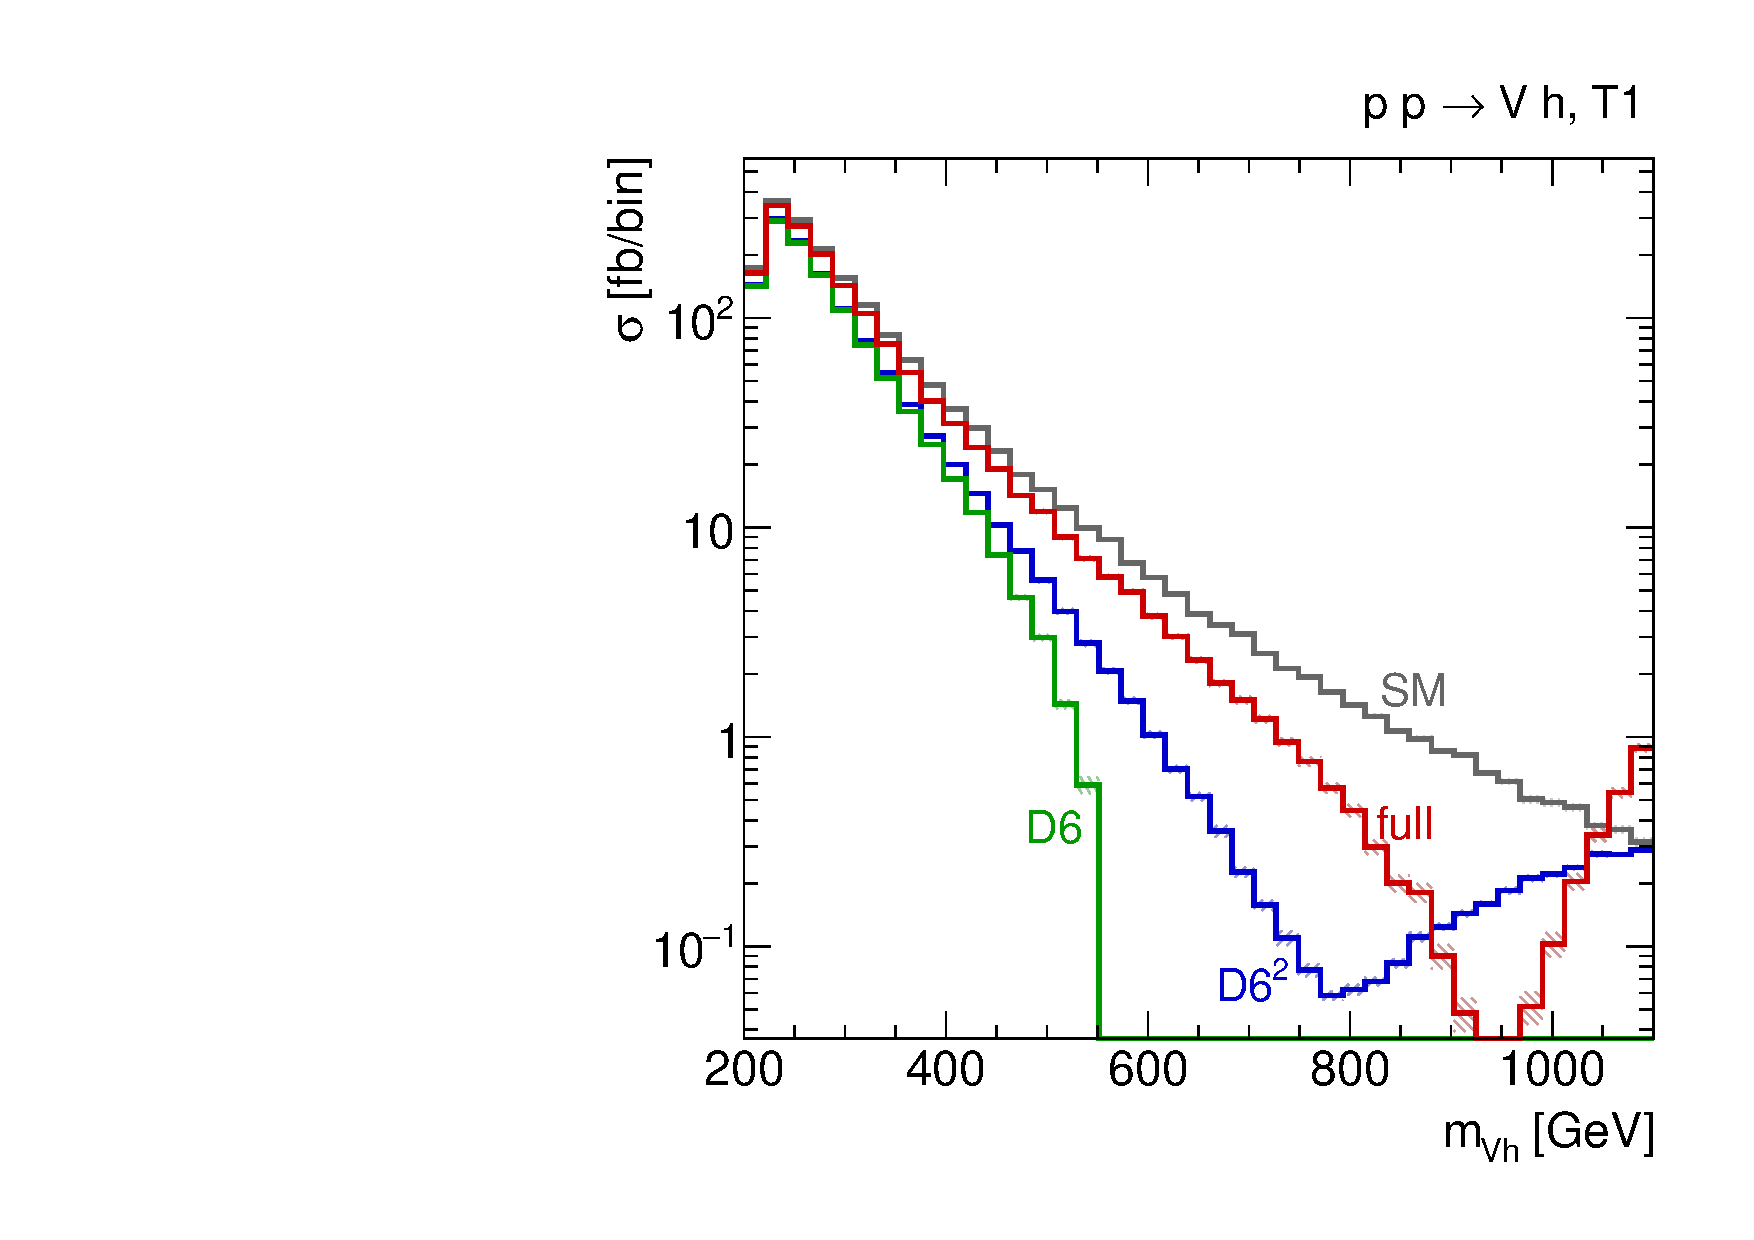
\includegraphics[width=0.43\textwidth]{fig/validity/VH_T1_mVH.pdf}
  \hspace*{0.05\textwidth}
  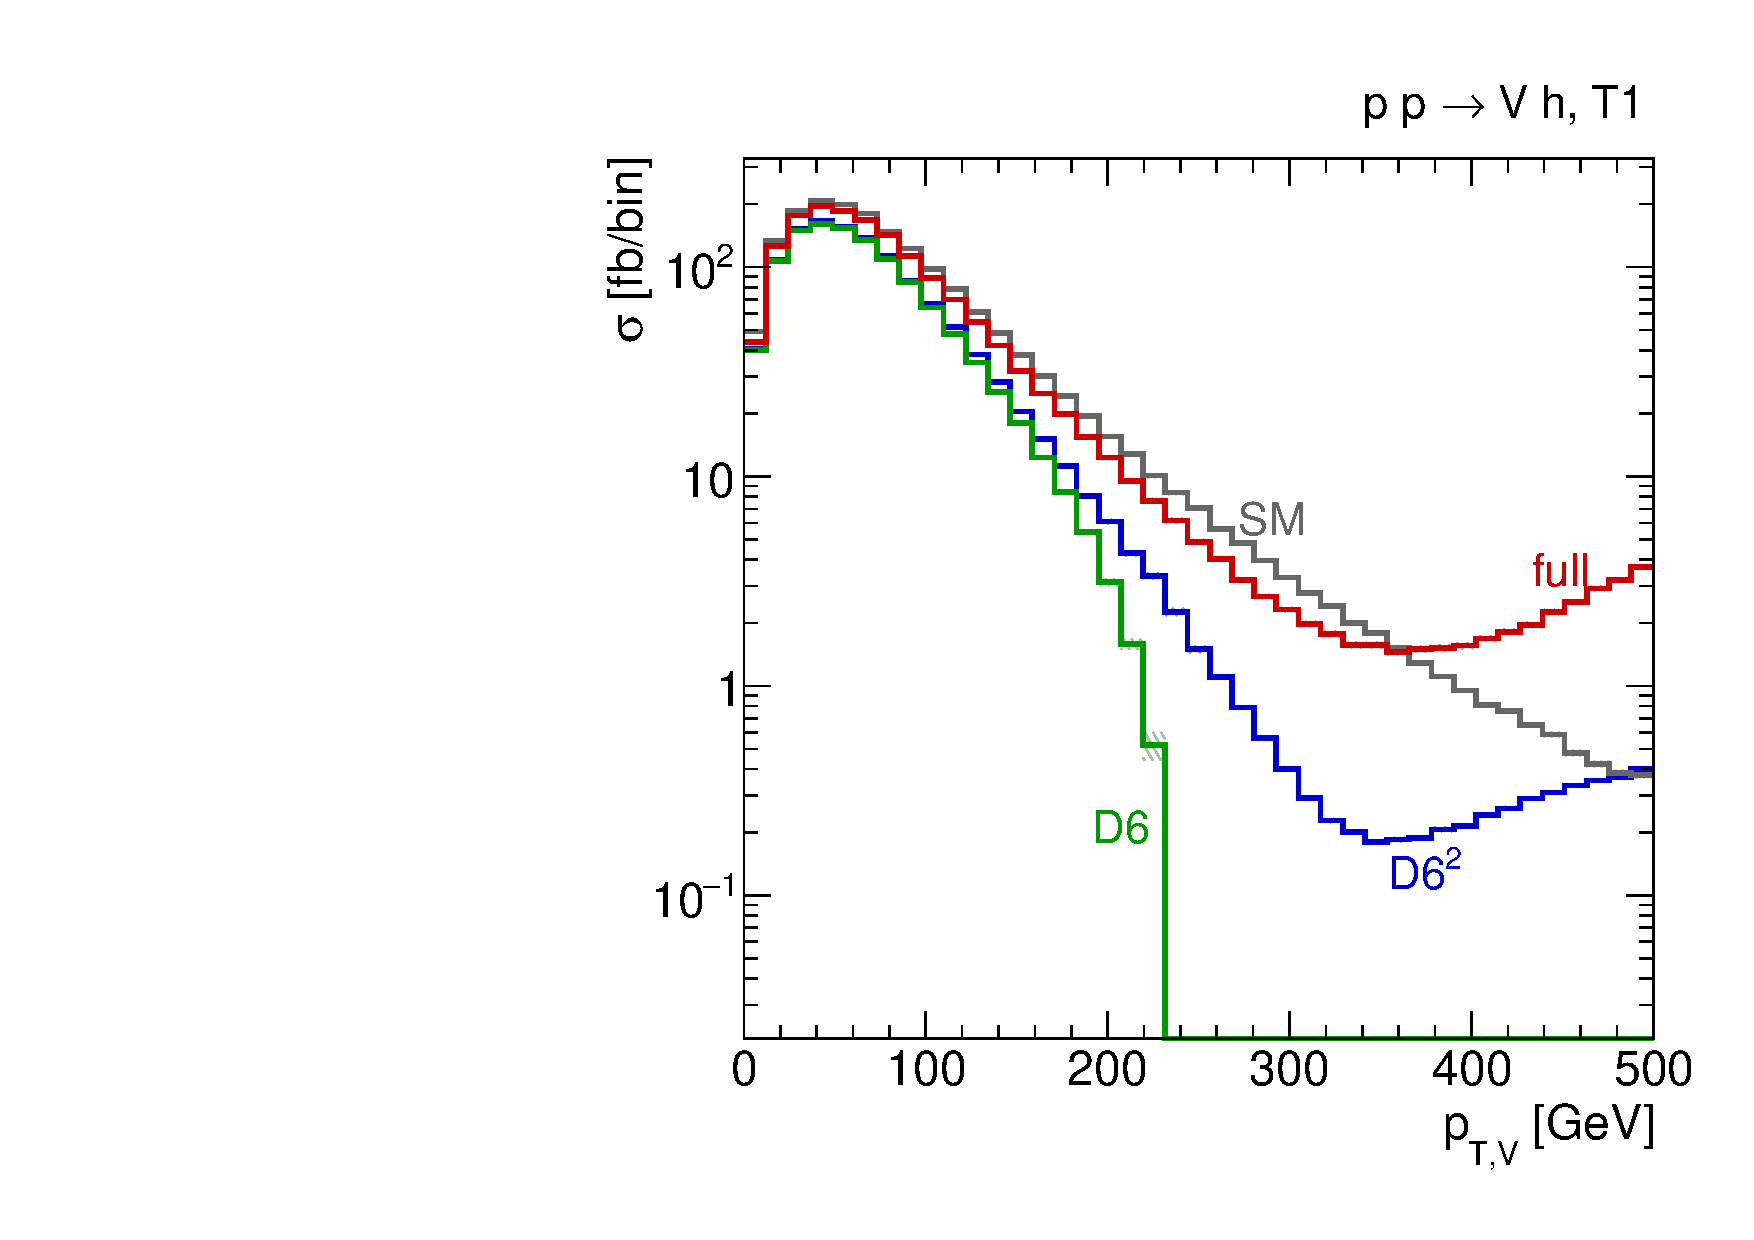
\includegraphics[width=0.43\textwidth]{fig/validity/VH_T1_Vpt.pdf} \\
  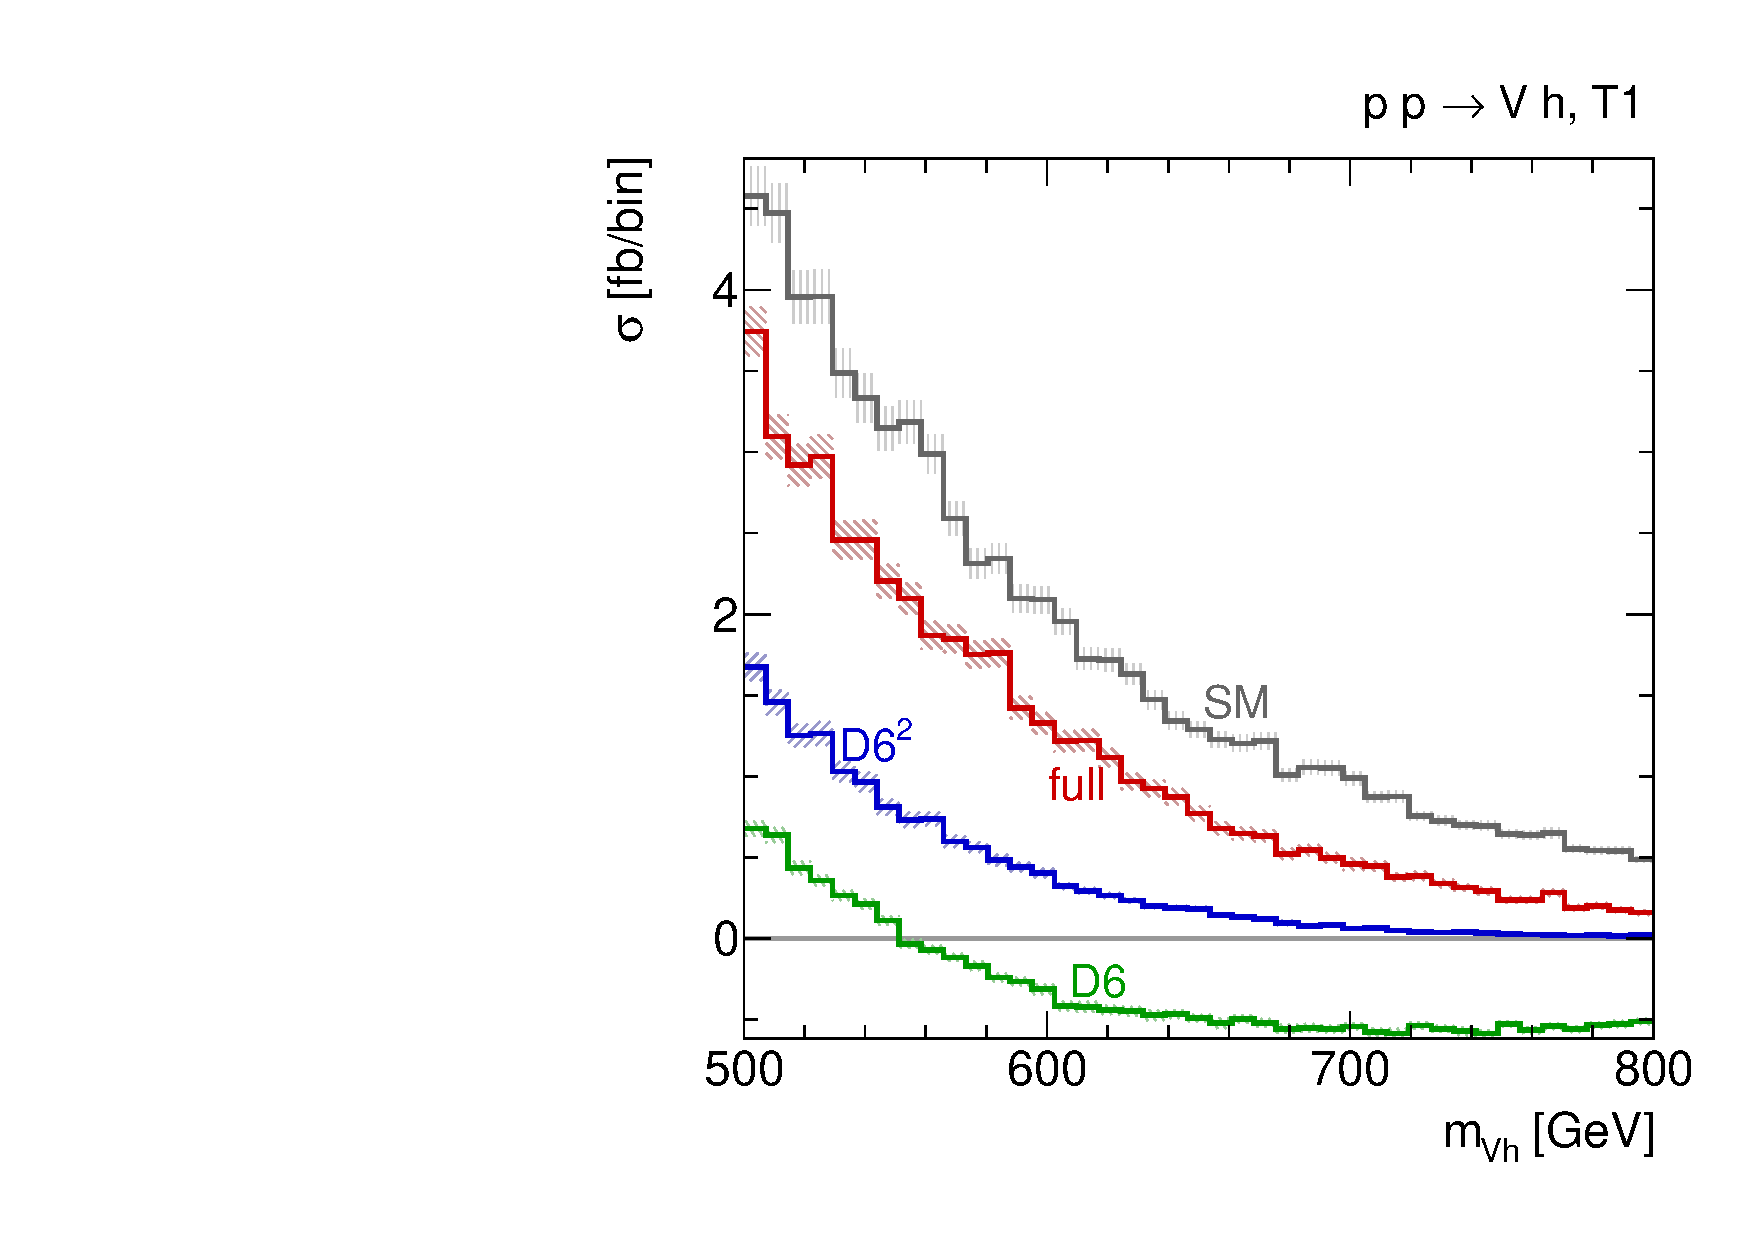
\includegraphics[width=0.43\textwidth]{fig/validity/VH_T1_mVH_zoom.pdf} 
  \hspace*{0.05\textwidth}
  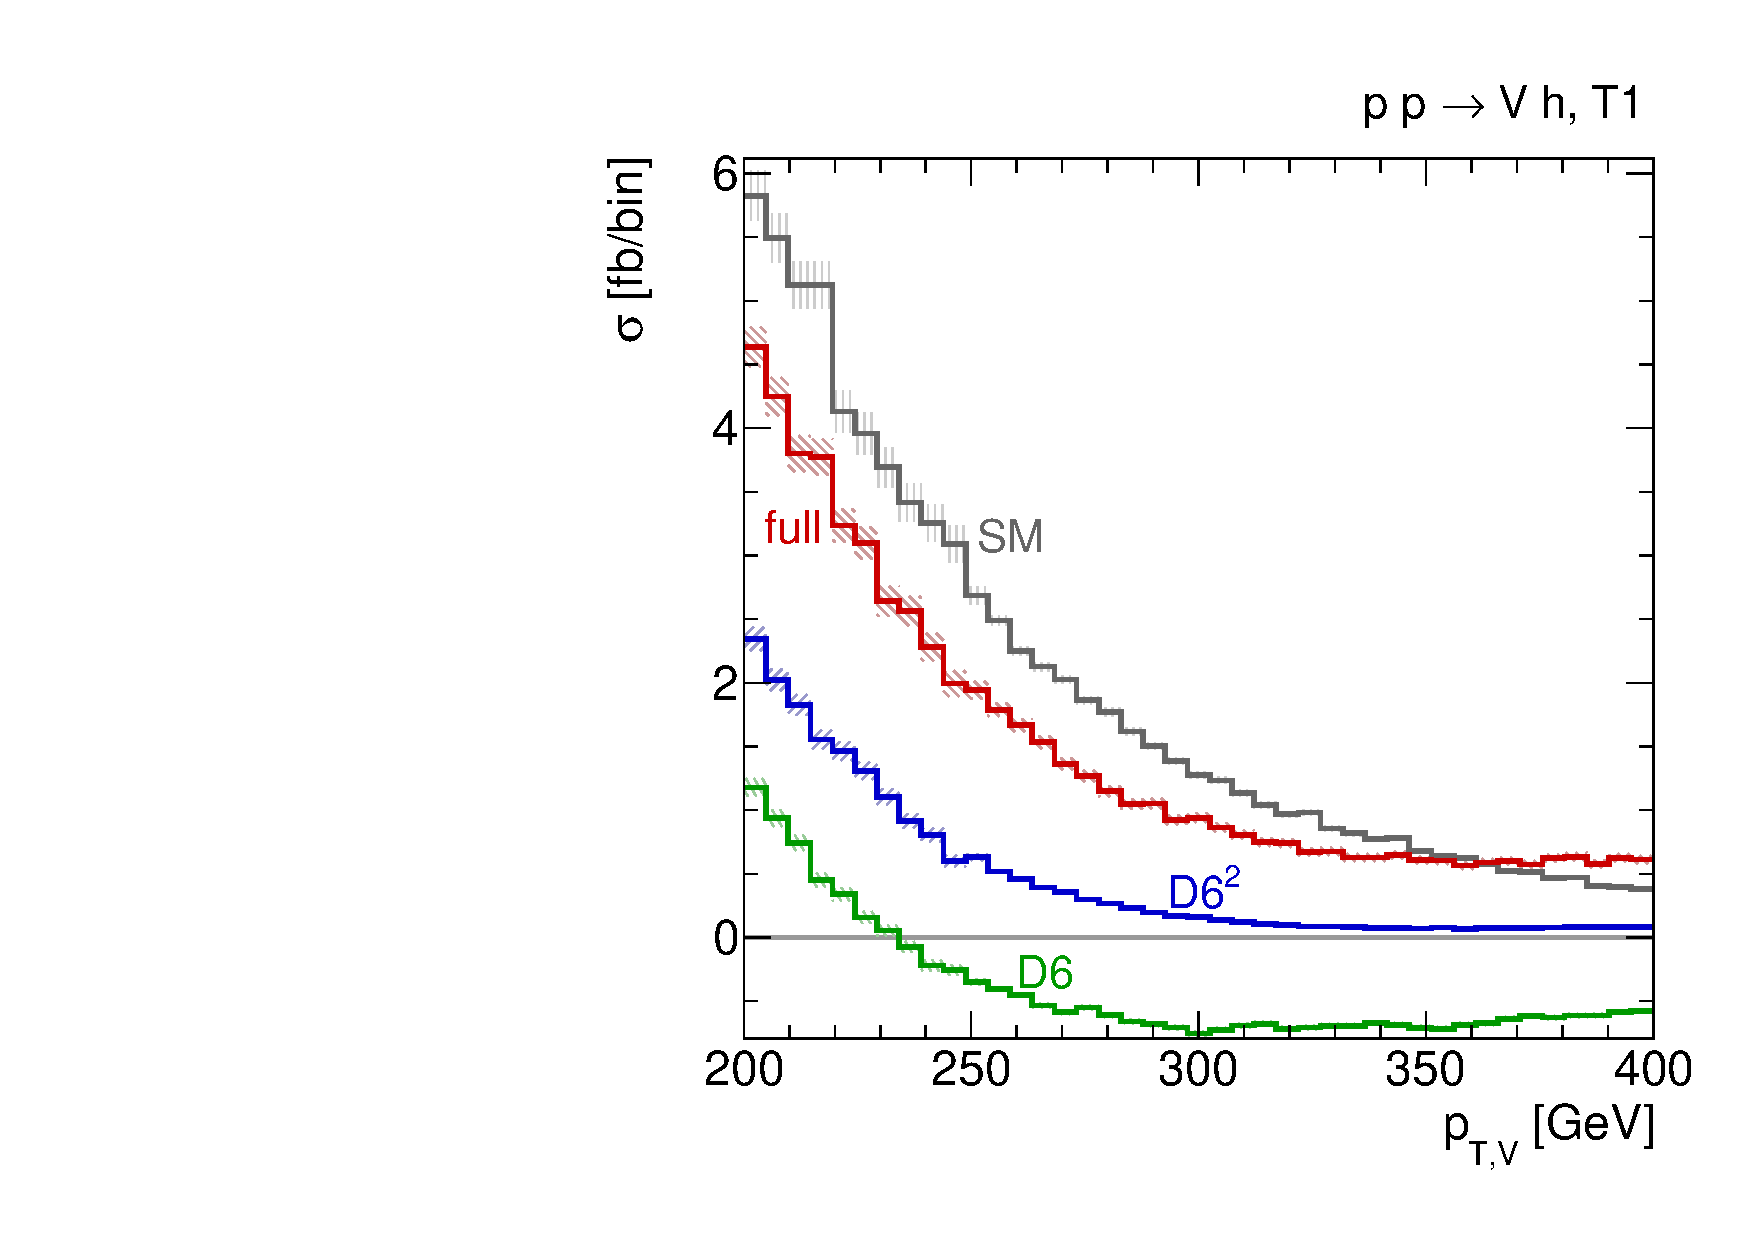
\includegraphics[width=0.43\textwidth]{fig/validity/VH_T1_Vpt_zoom} \\
  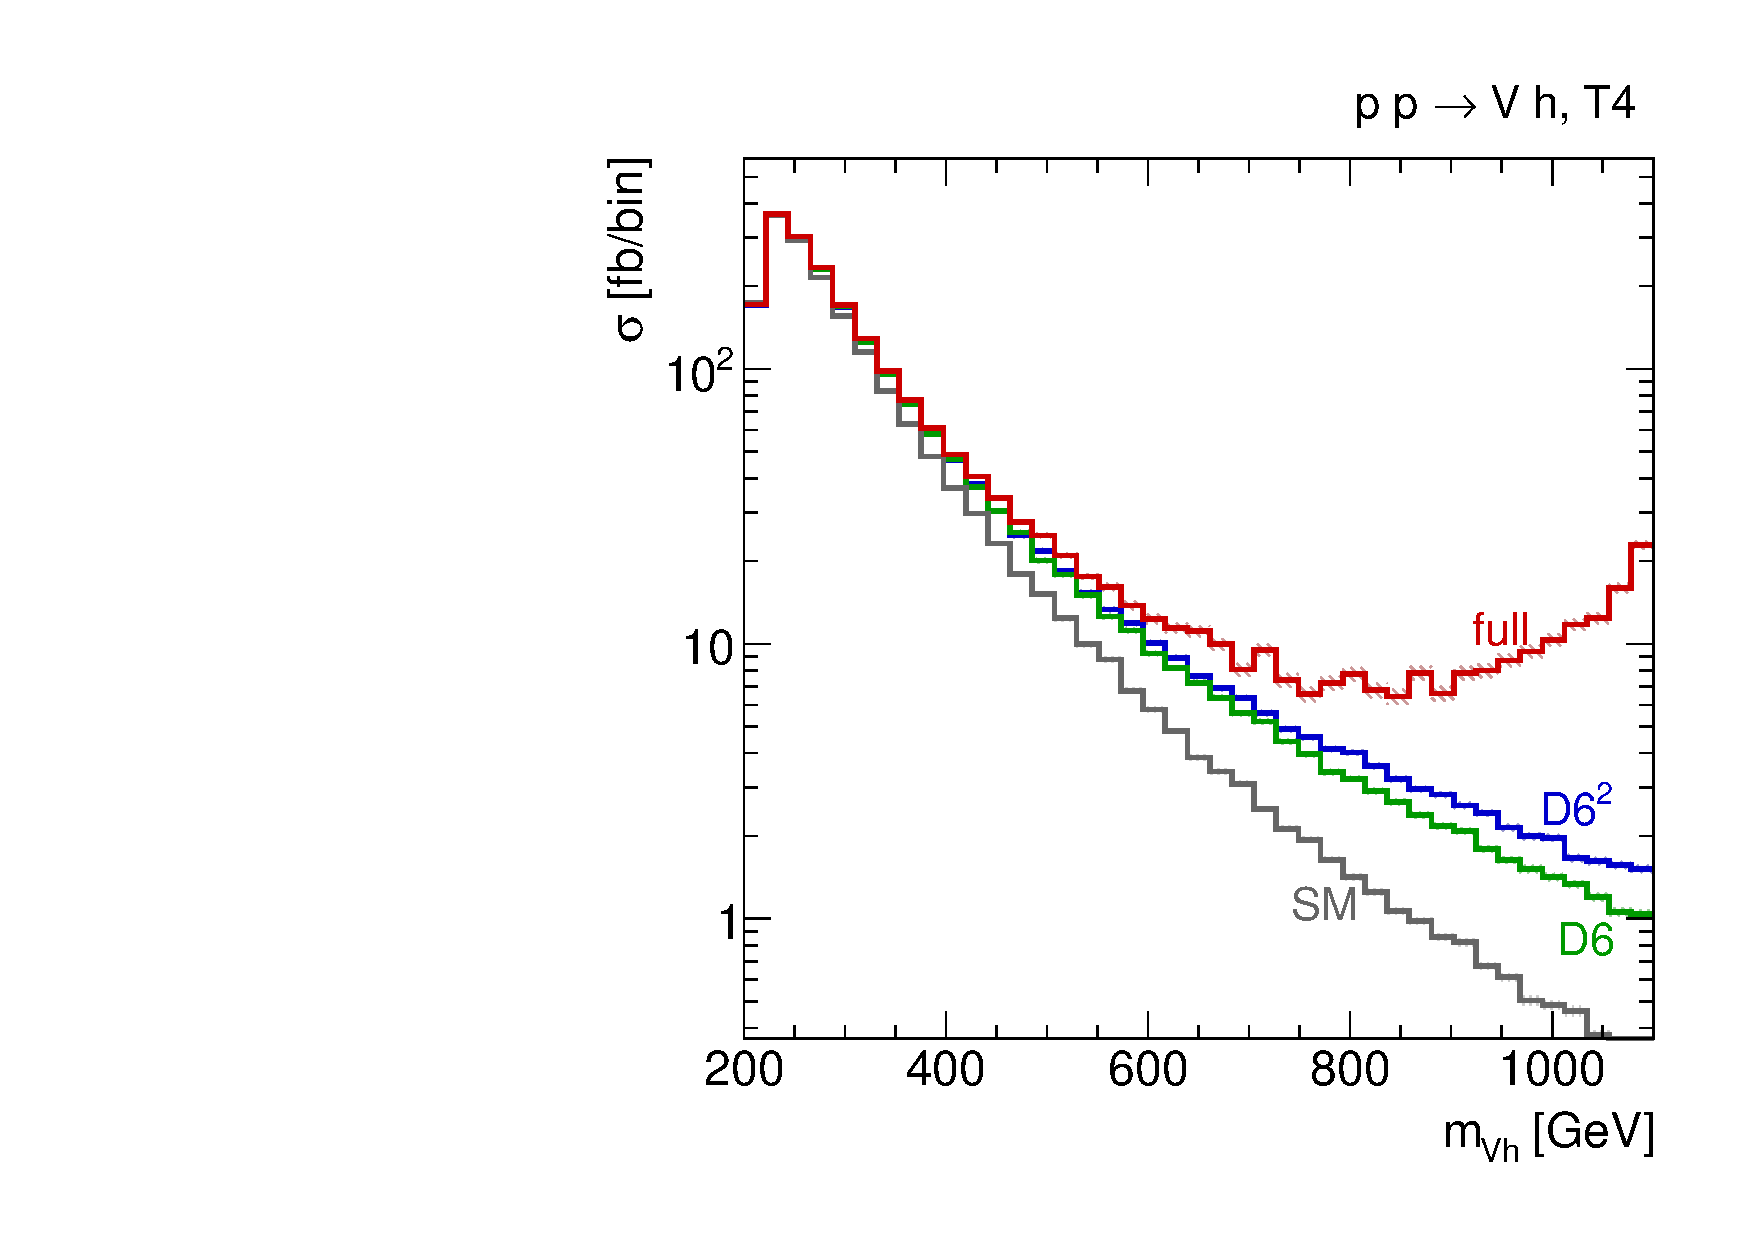
\includegraphics[width=0.43\textwidth]{fig/validity/VH_T4_mVH}
  \hspace*{0.05\textwidth}
  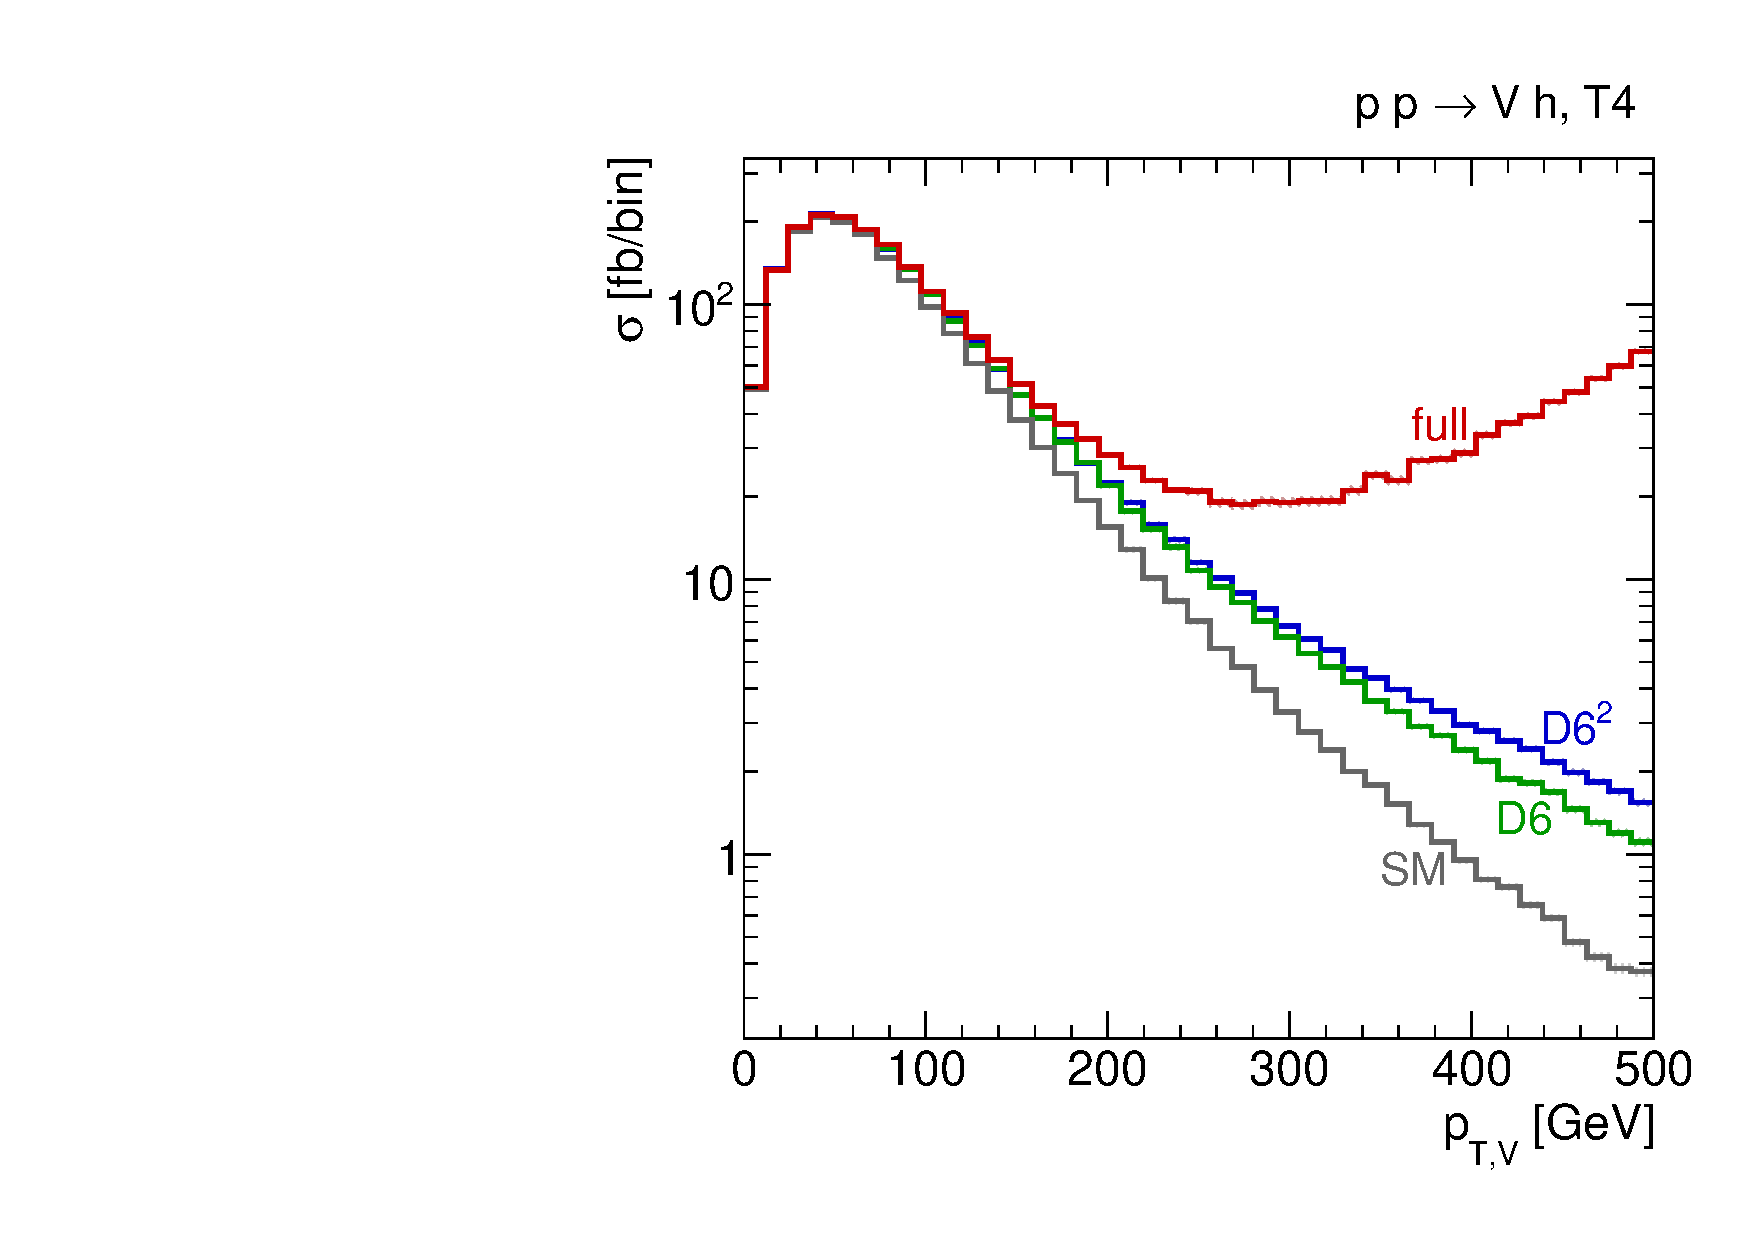
\includegraphics[width=0.43\textwidth]{fig/validity/VH_T4_Vpt}
  \caption{$Vh$ distributions with (``D6$^{2}$'') and without (``D6'')
    the dimension-six squared
    term. The left panels show $m_{VH}$, the right panels
    $p_{T,V}$. The central panels show the region where leaving out
    the squared dimension-six terms leads to a negative cross section.}
  \label{fig:validity_squared_VH}
\end{figure}
%------------------------------------------------------------


%%%%%%%%%%%%%%%%%%%%%%%%%%%%%%%%%%%%%%%%%%%%%%%%%%%%%%%%%%%%
\subsubsection*{WBF Higgs production}
%%%%%%%%%%%%%%%%%%%%%%%%%%%%%%%%%%%%%%%%%%%%%%%%%%%%%%%%%%%%

Weak-boson-fusion Higgs production is a $2 \to 3$ process with two
$t$-channel gauge bosons carrying the momentum to the Higgs vertex.
The relevant kinematic variables are the two virtualities of the weak
bosons. Following many studies in the framework of the effective $W$
approximation~\cite{effective_w,polarized_ww} it is straightforward to
link them to the $p_T$ of the tagging jets, which even for multiple
jet radiation can be linked to the transverse momentum of the
Higgs~\cite{Buschmann:2014twa} (even though it is not clear if this
distribution is theoretically or experimentally favoured).  Again, we
start with the parton-level signal process
%
\begin{align}
u d \to u' d' h
\label{eq:validity_def_wbf}
\end{align}
%
with only one minimal cut $p_{T,j} > 20$~GeV for the two tagging jets.  We
show the results for the now constructively interfering benchmark
point T1 and the now destructively interfering benchmark point T4 in
\autoref{fig:validity_squared_WBF}. Negative event rates for T4 appear around
%
\begin{align}
p_{T,j_1} > 600~\gev \approx \frac{m_\xi^\text{(T4)}}{2} \; , 
\label{eq:validity_breakdown_wbf}
\end{align}
%
forcing us to either disregard the corresponding model hypothesis or
to add the dimension-six squared term.  For the less critical point T1
the agreement between the vector triplet model and its dimension-six
approximation including the squared terms extends well into the range
where deviations from the Standard Model become visible.

%------------------------------------------------------------
\begin{figure}
  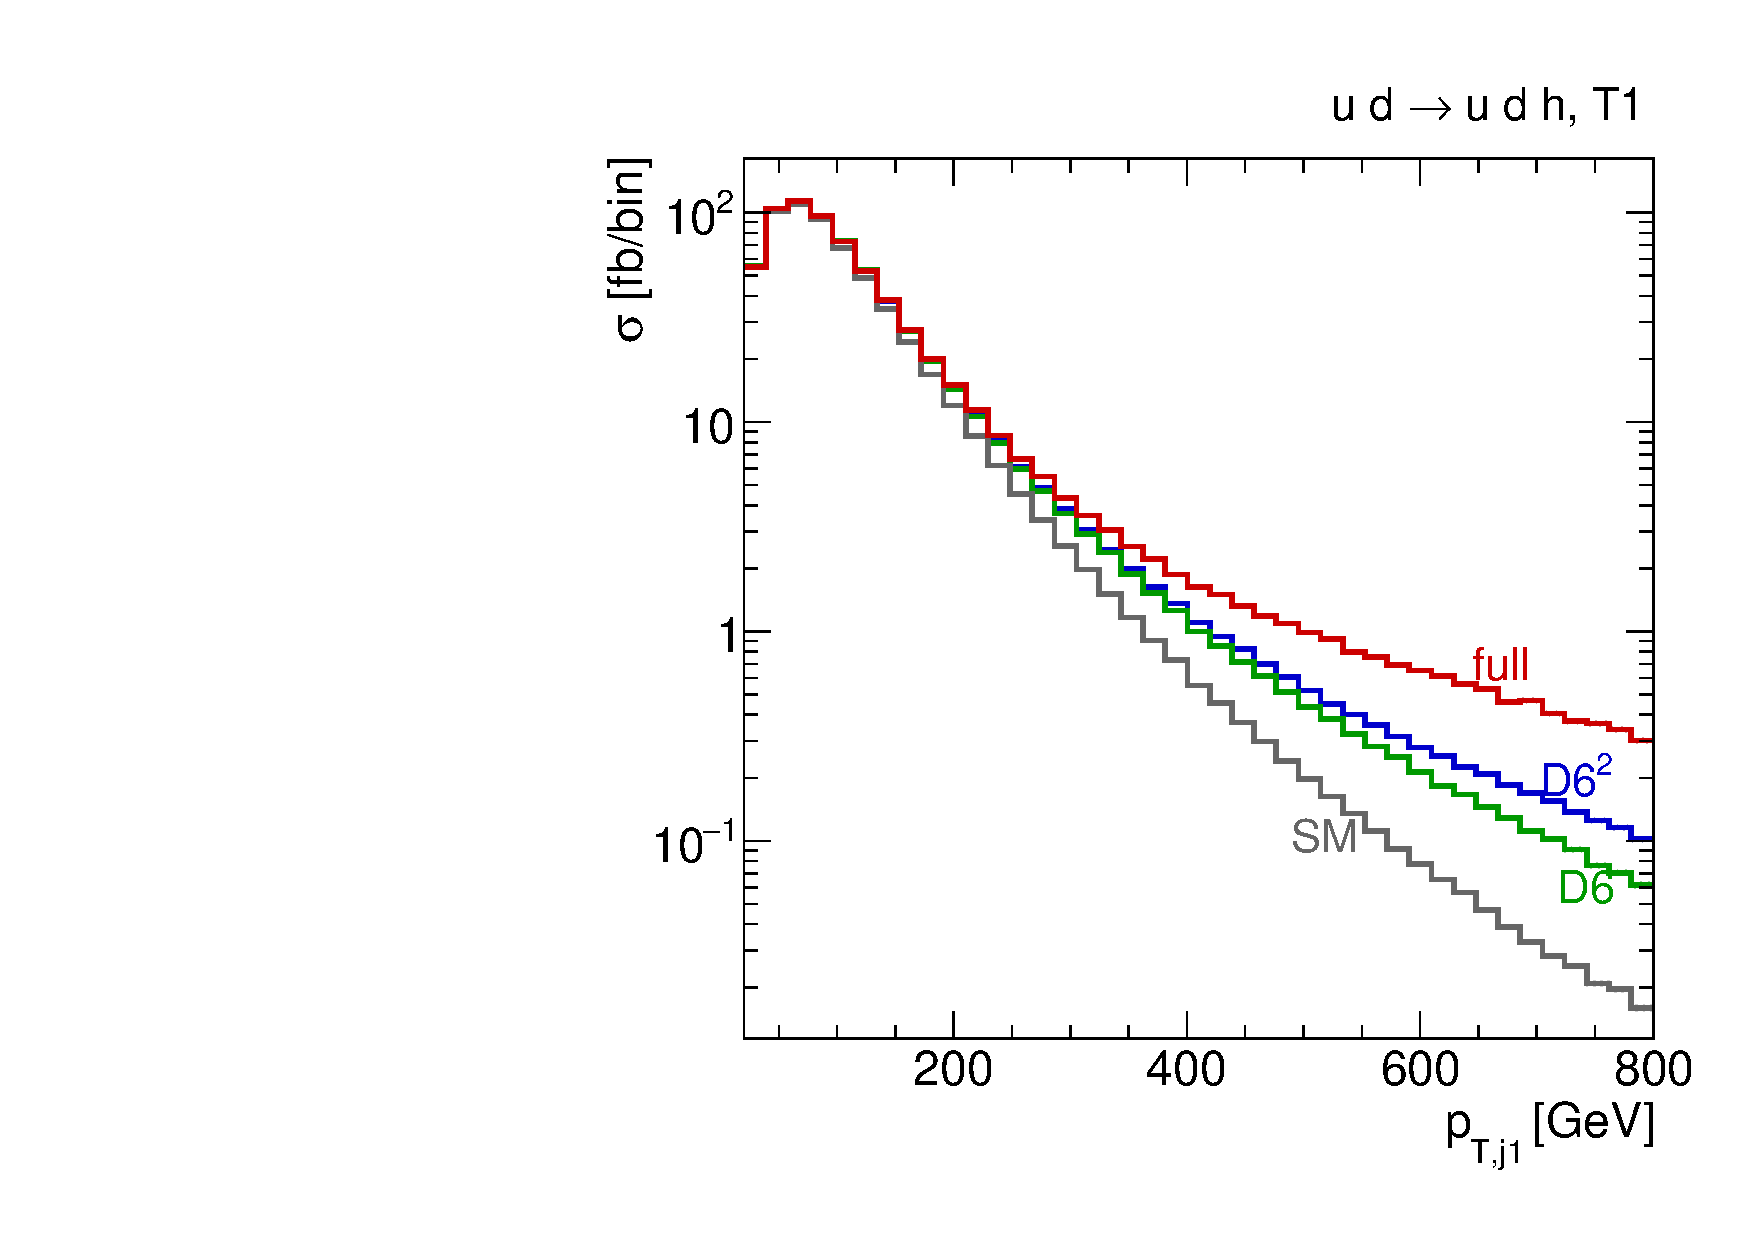
\includegraphics[width=0.43\textwidth]{fig/validity/WBF_T1_j1pt.pdf} 
  \hspace*{0.05\textwidth}
  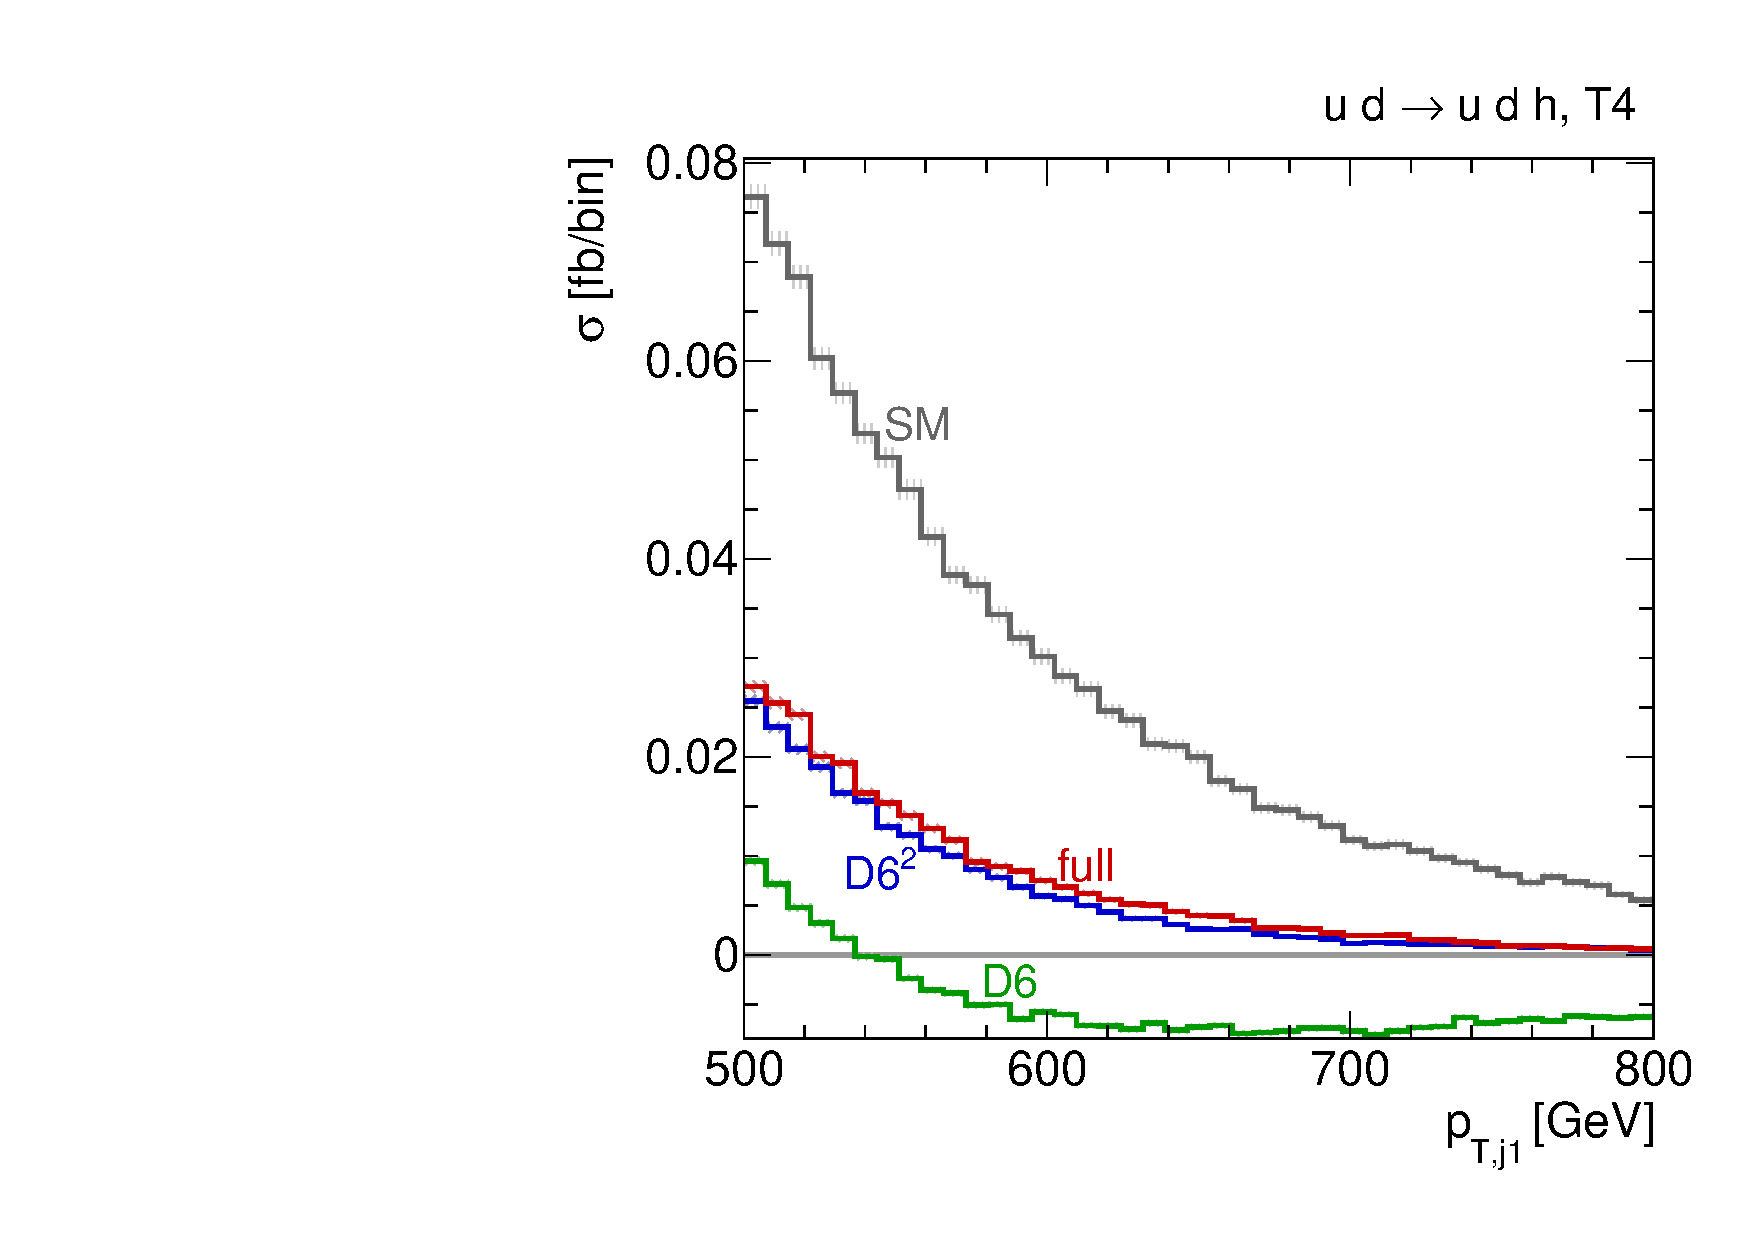
\includegraphics[width=0.43\textwidth]{fig/validity/WBF_T4_j1pt_zoom.pdf}\\
  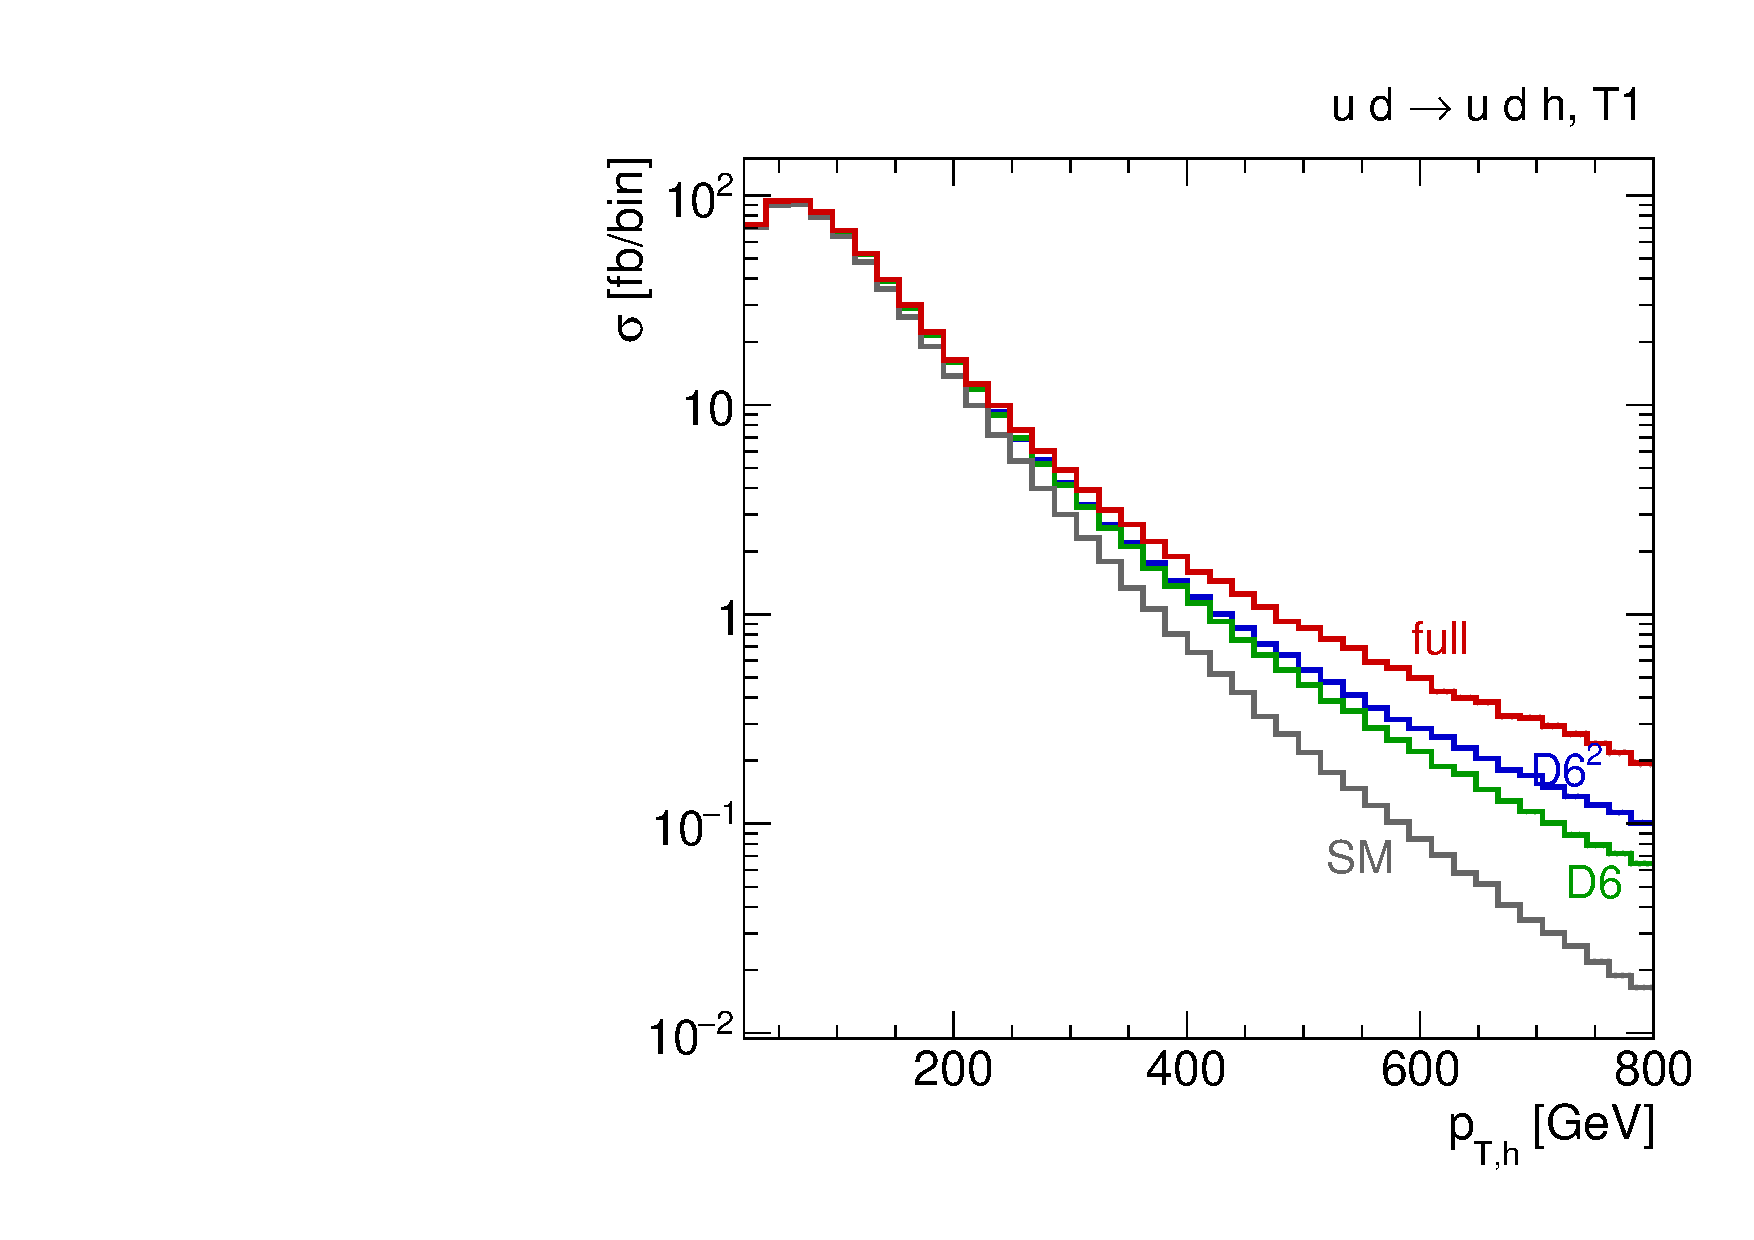
\includegraphics[width=0.43\textwidth]{fig/validity/WBF_T1_Hpt.pdf} 
  \hspace*{0.05\textwidth}
  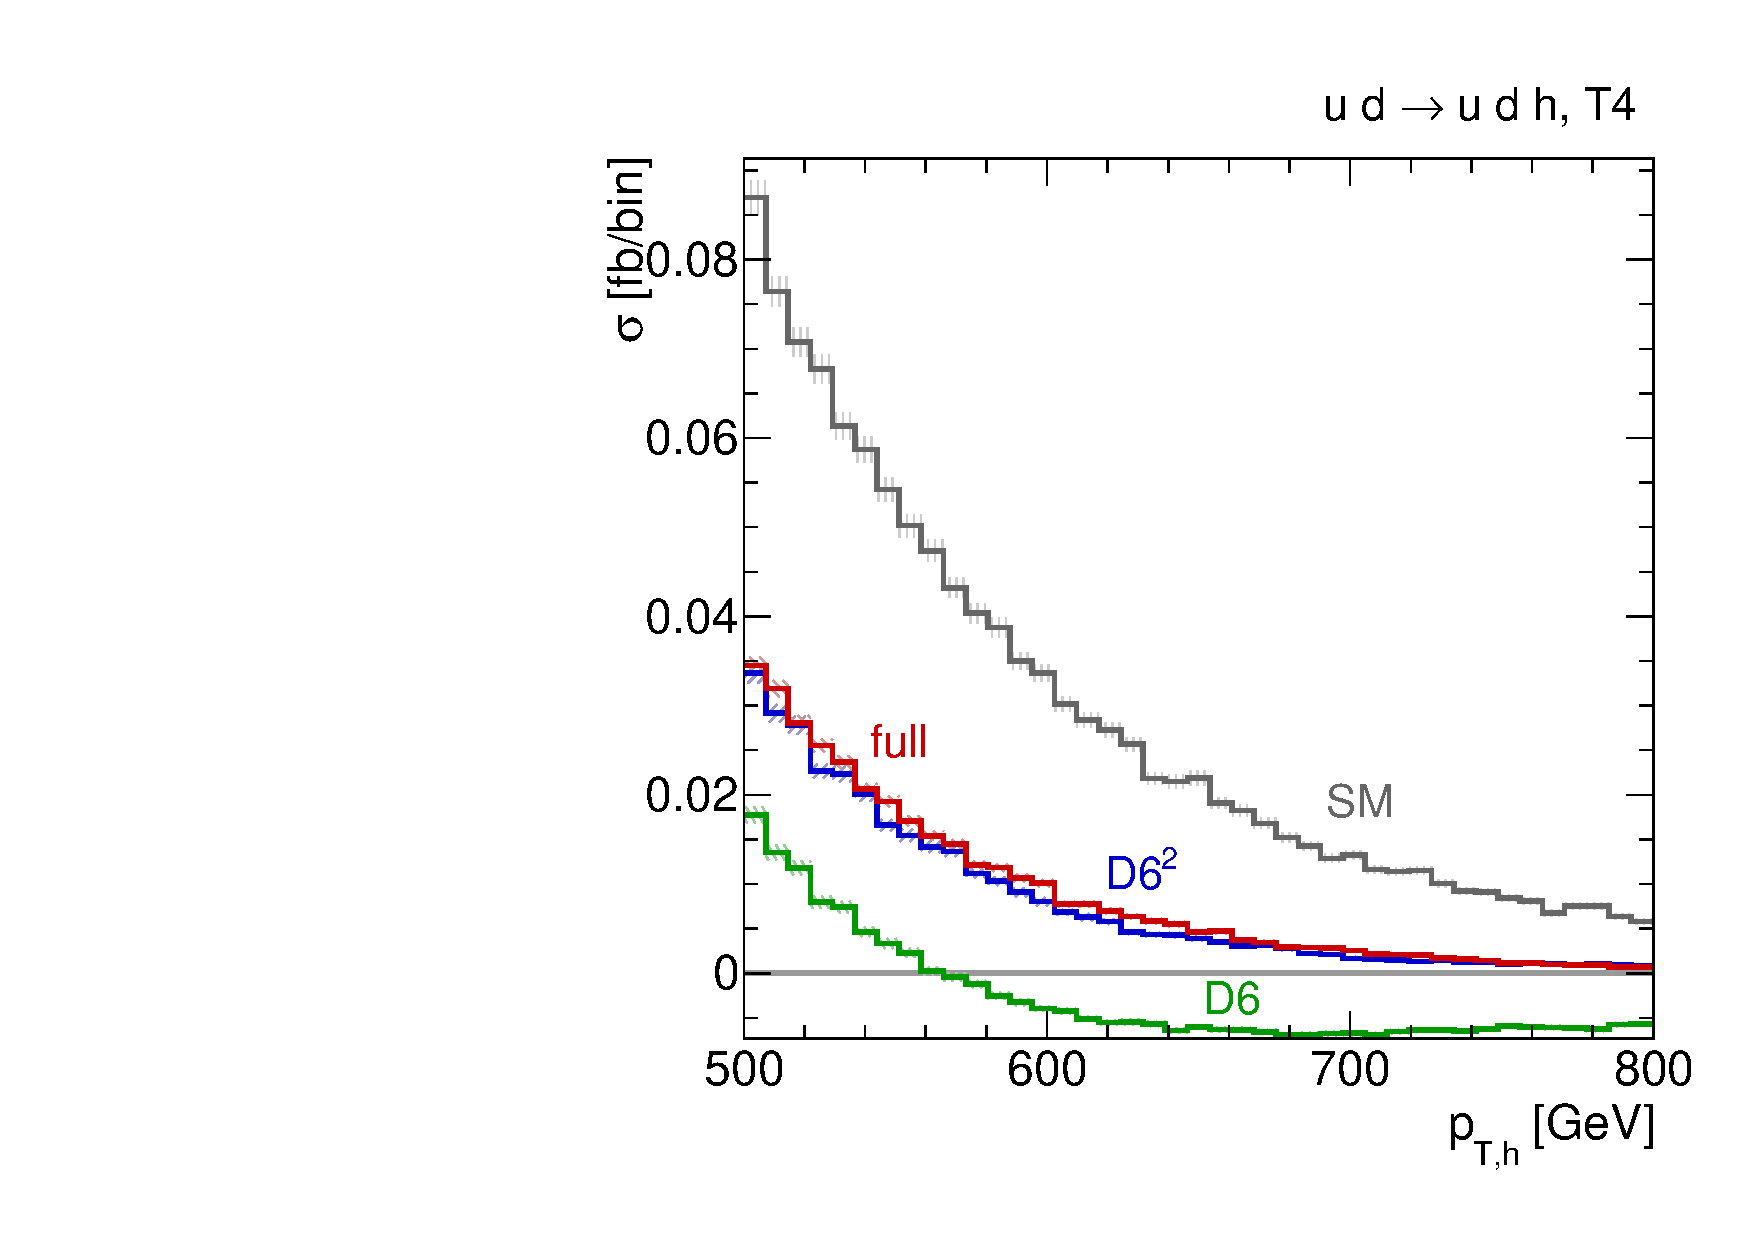
\includegraphics[width=0.43\textwidth]{fig/validity/WBF_T4_Hpt.pdf}\\
  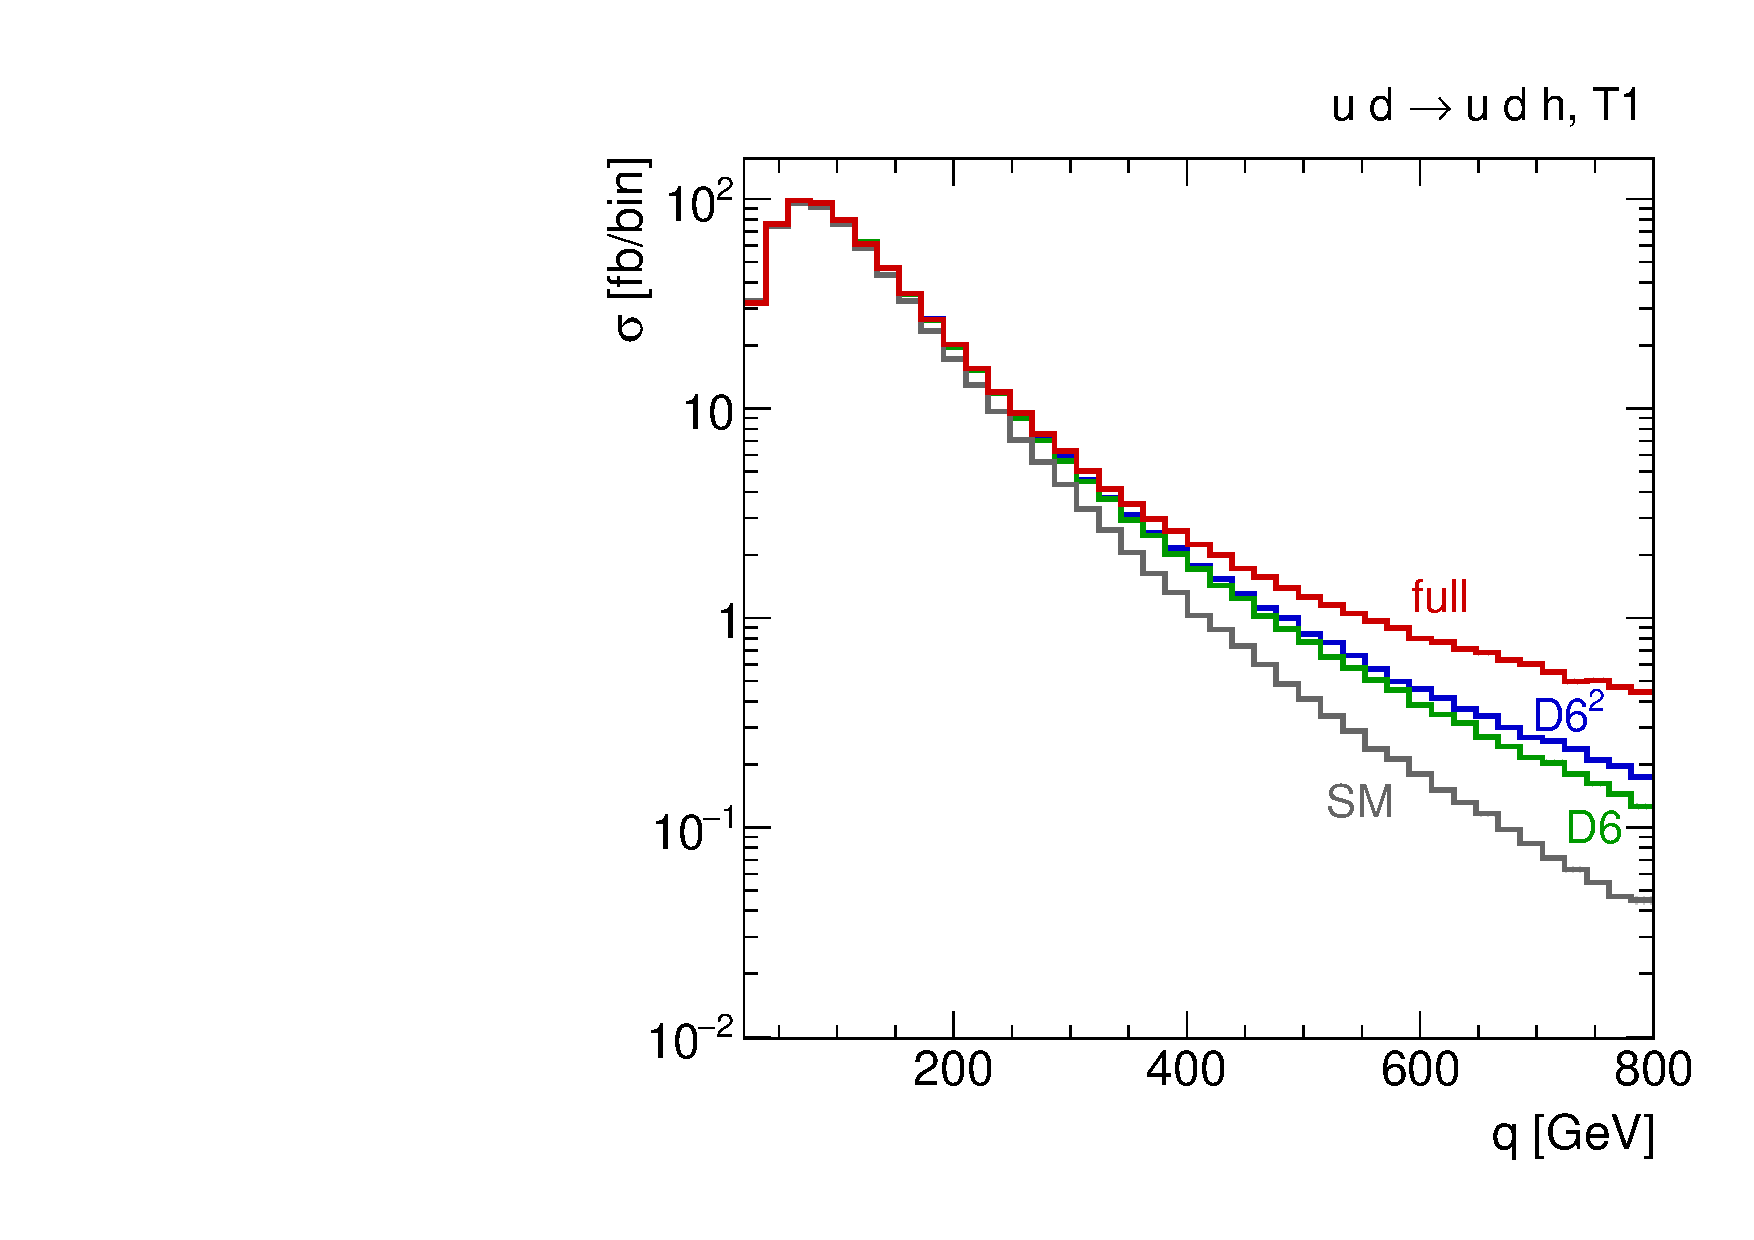
\includegraphics[width=0.43\textwidth]{fig/validity/WBF_T1_q.pdf} 
  \hspace*{0.05\textwidth}
  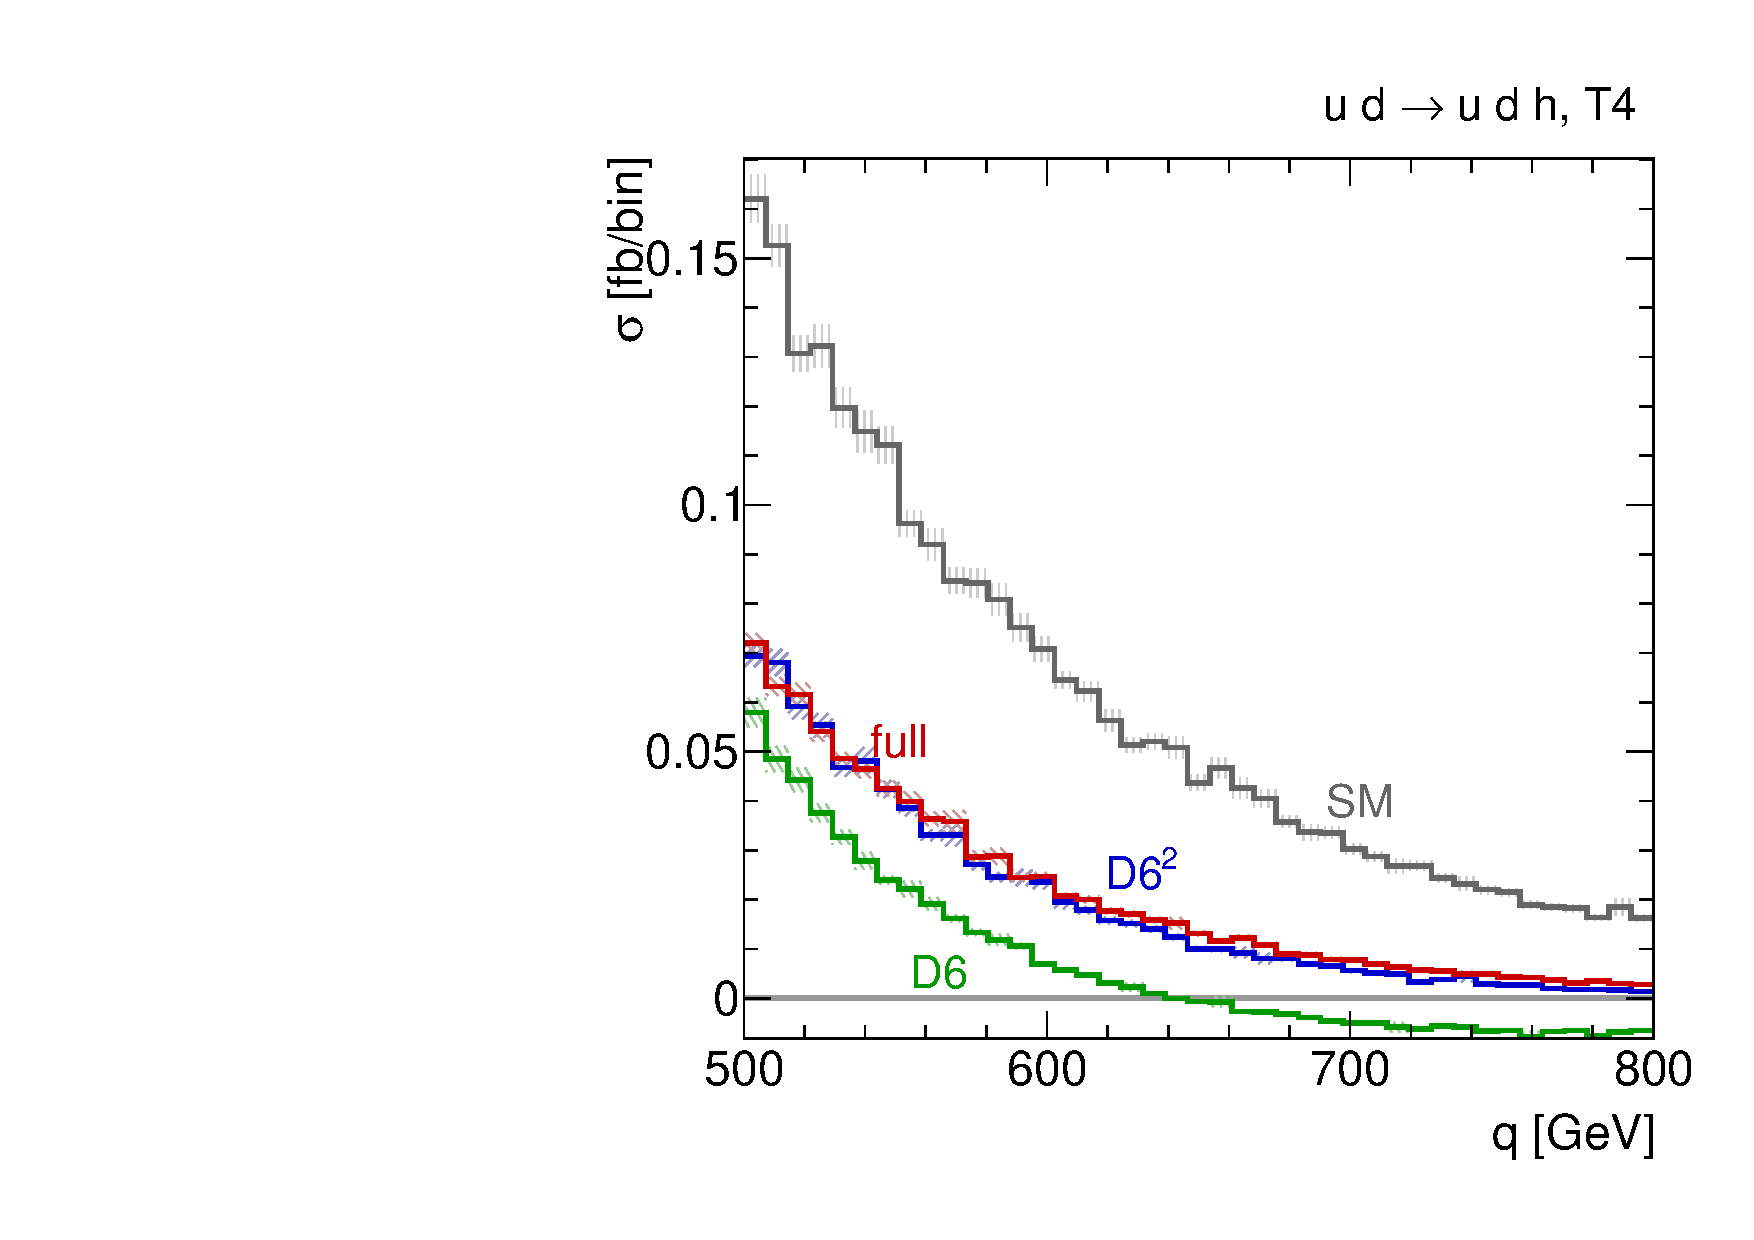
\includegraphics[width=0.43\textwidth]{fig/validity/WBF_T4_q.pdf}
  \caption{WBF distributions with (``D6$^{2}$'') and without (``D6'') the
    dimension-six squared term. From top to bottom: $p_{T,j1}$, $p_{T,h}$, and
    virtuality $q$ defined in Equation\;\eqref{eq:validity_virt}. The right panels show the region where
    leaving out the squared dimension-six terms leads to a negative cross
    section.}
  \label{fig:validity_squared_WBF}
\end{figure}
%------------------------------------------------------------


%------------------------------------------------------------
\begin{figure}[t]
  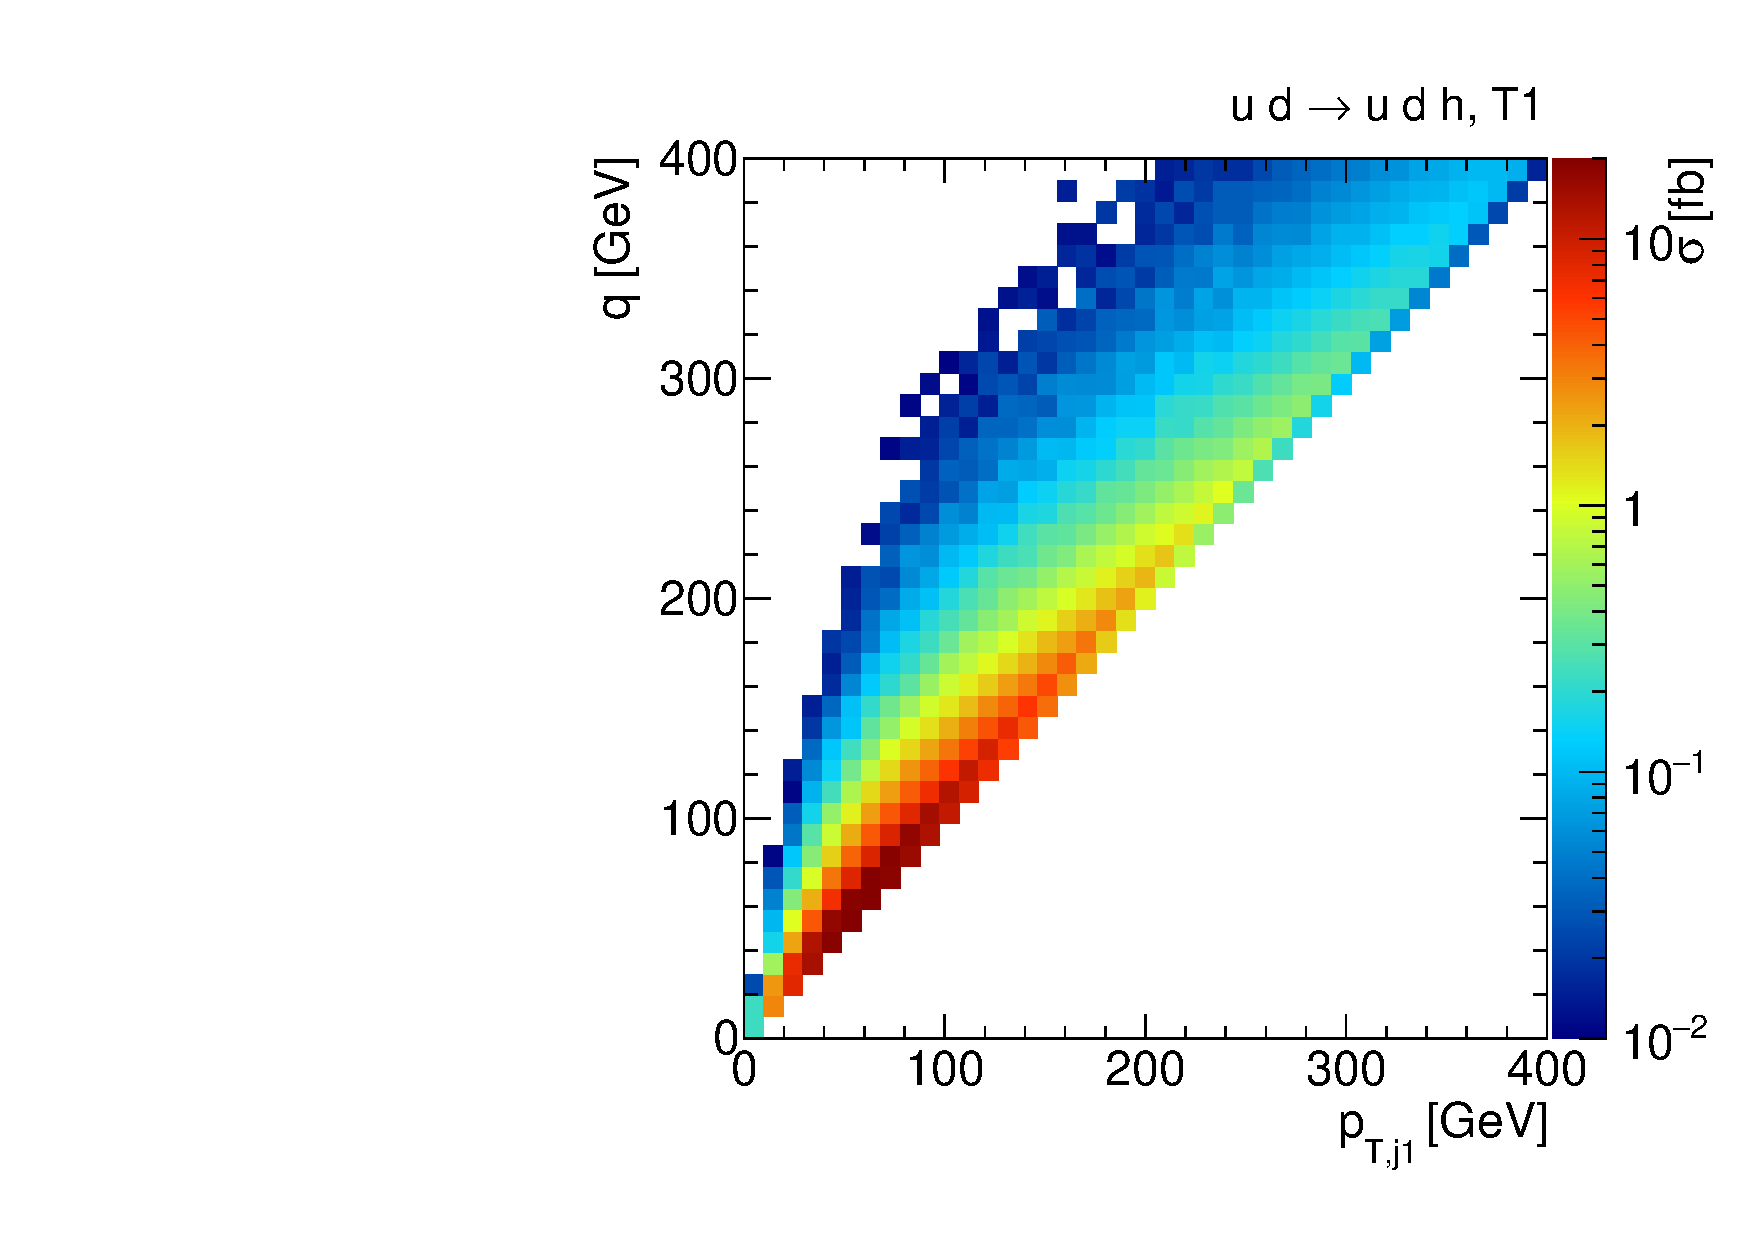
\includegraphics[width=0.43\textwidth]{fig/validity/WBF_correl_q_j1pt.pdf}
  \hspace*{0.05\textwidth}
  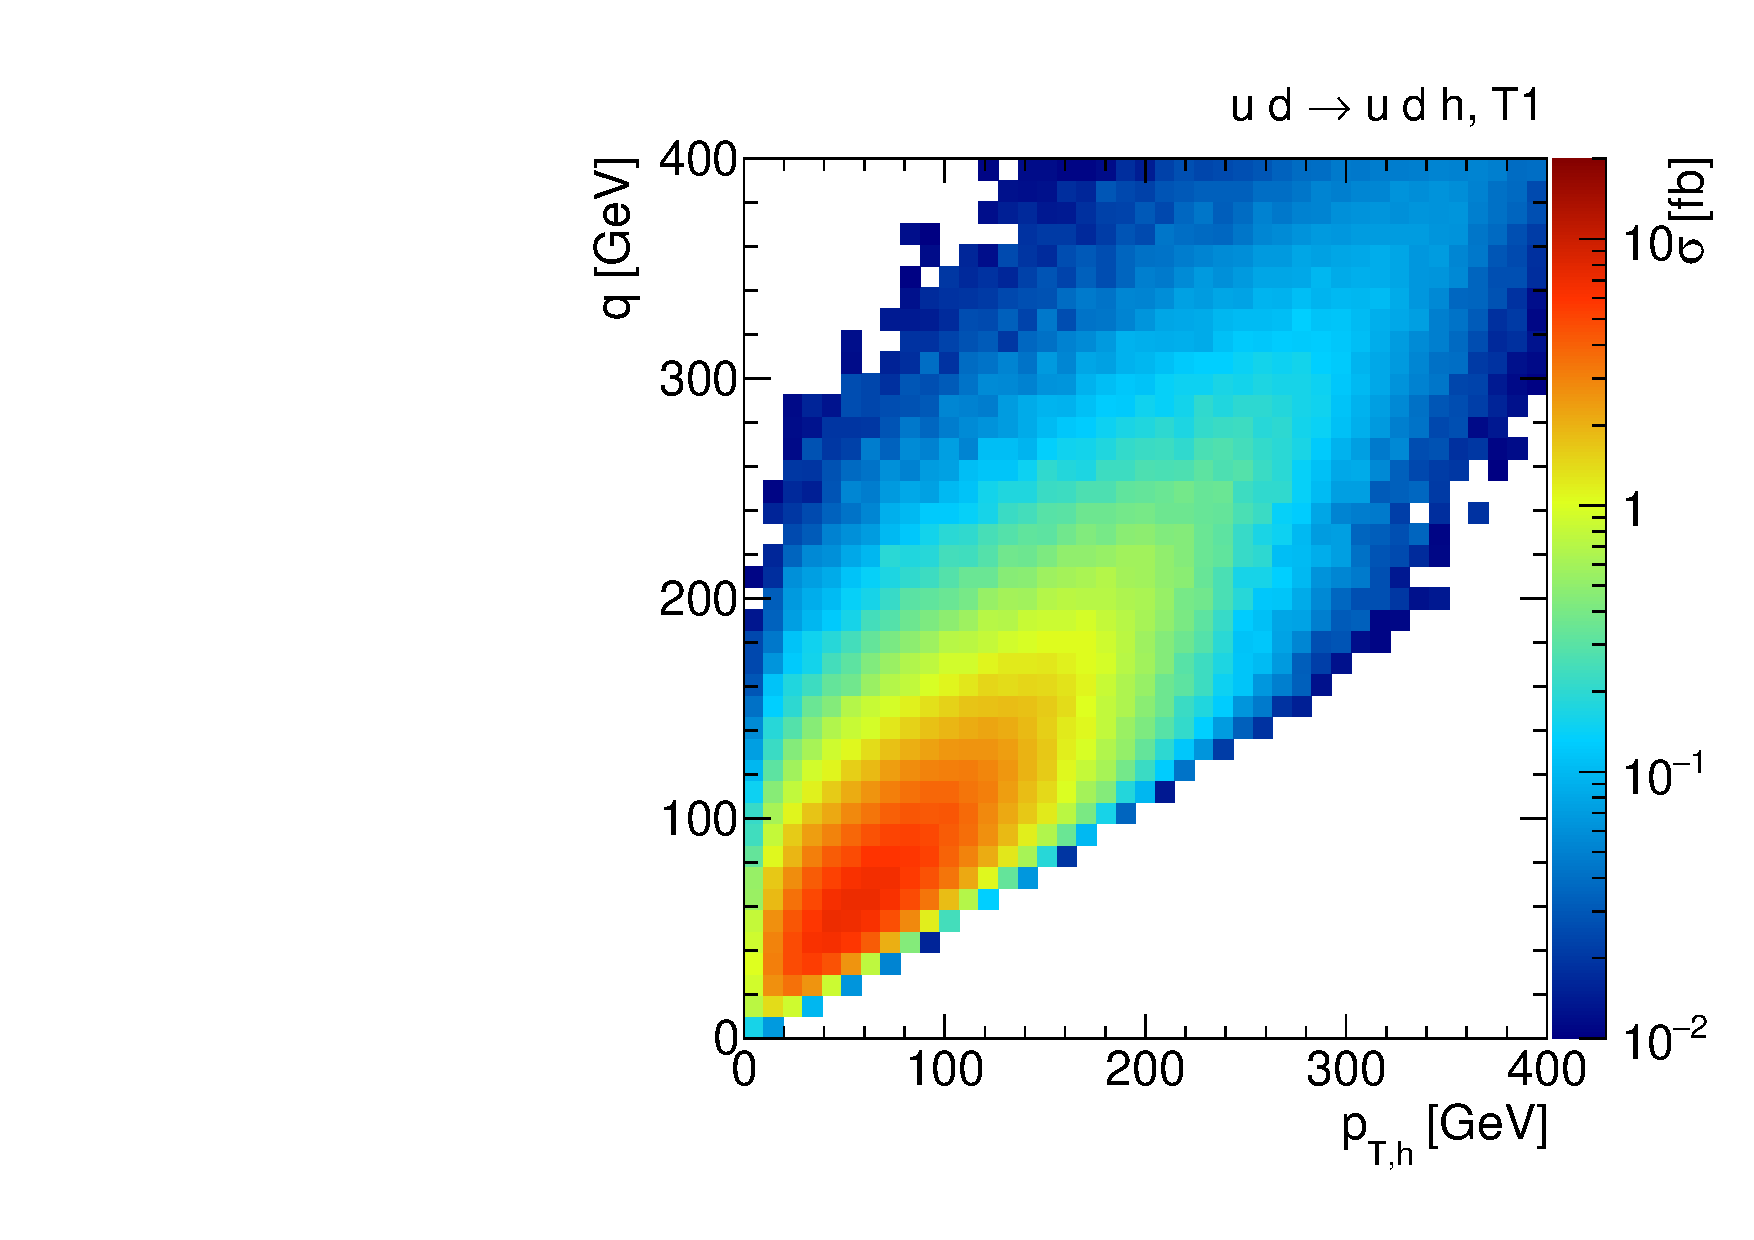
\includegraphics[width=0.43\textwidth]{fig/validity/WBF_correl_q_Hpt.pdf} 
  \caption{WBF correlations between the virtuality $q$ and
    $p_{T,j_1}$ (left) or $p_{T,h}$ (right).}
  \label{fig:validity_virt_corr}
\end{figure}
%------------------------------------------------------------

%------------------------------------------------------------
\begin{figure}[b!]
  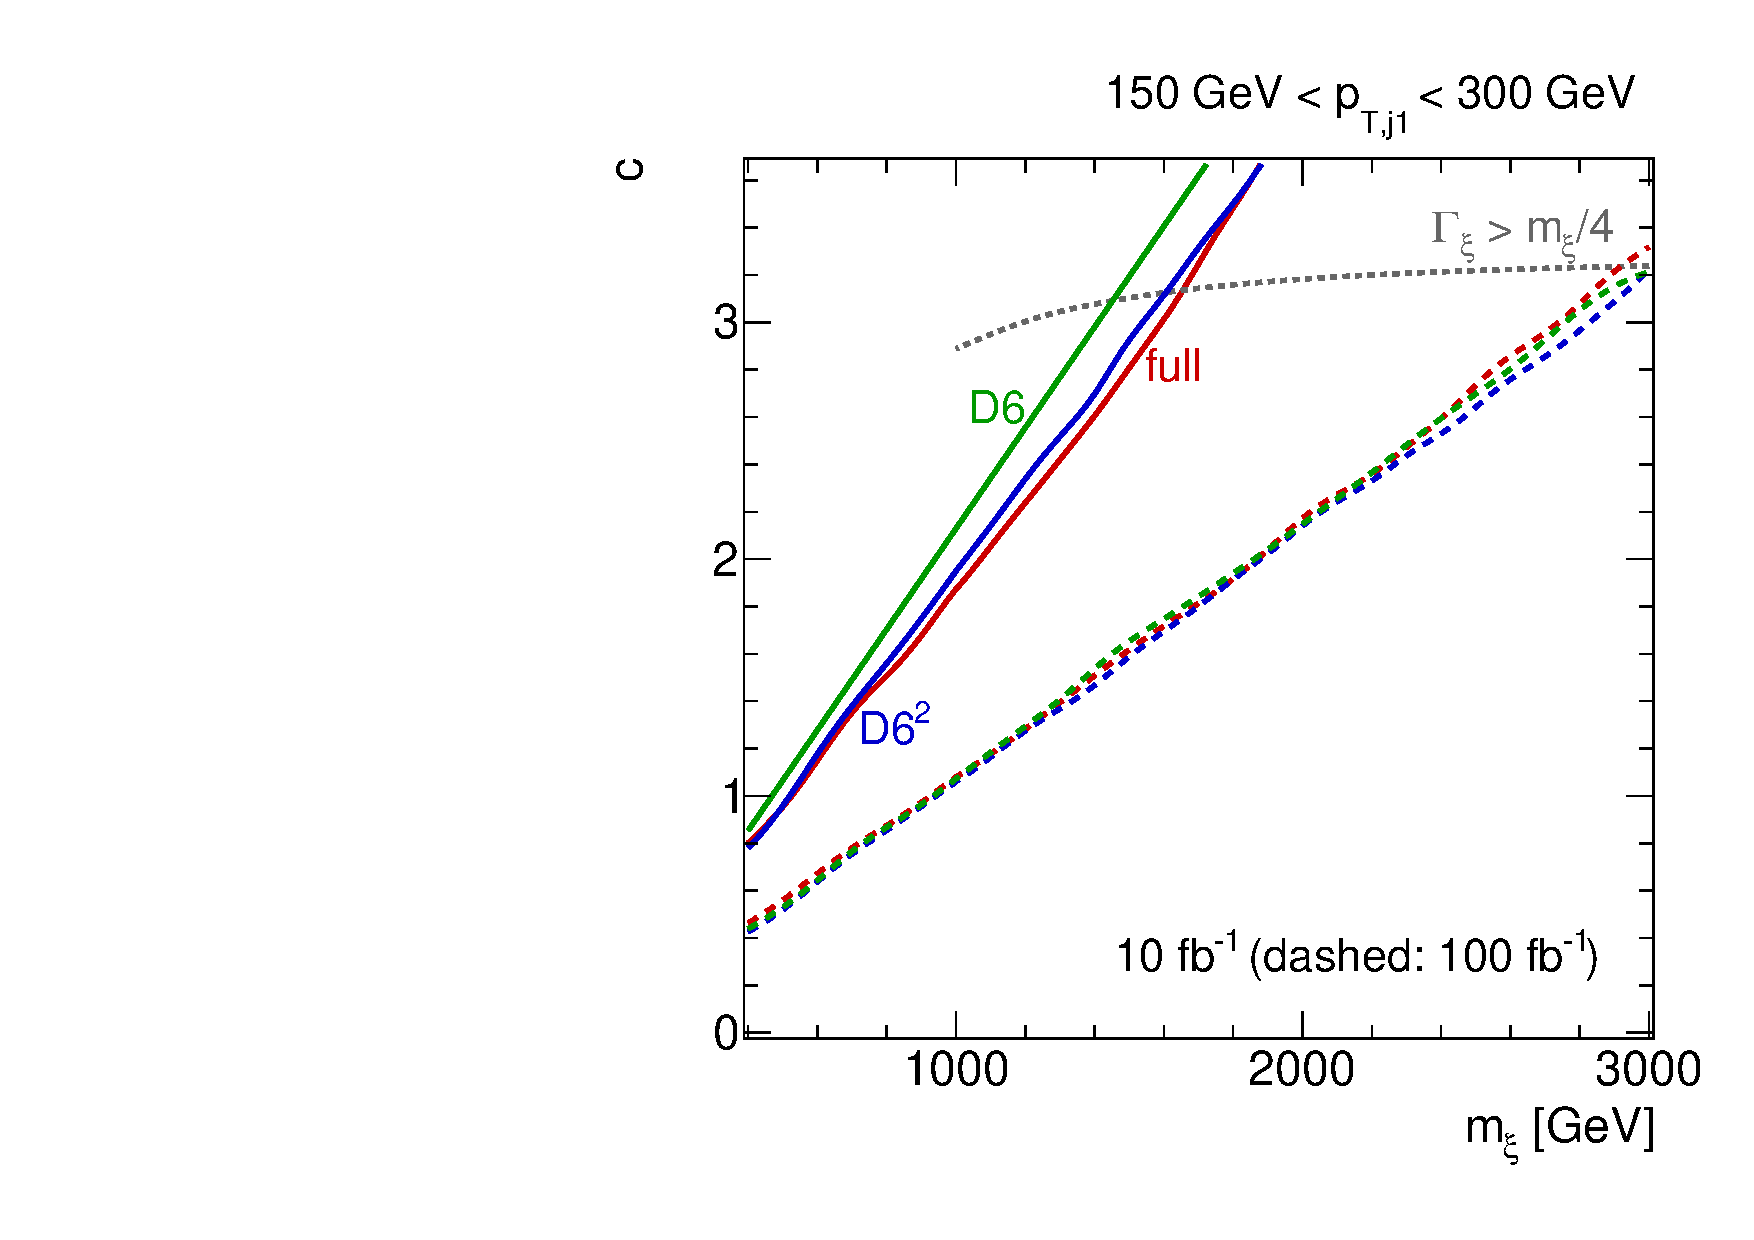
\includegraphics[width=0.43\textwidth]{fig/validity/WBF_limits_150.pdf}
  \hspace*{0.05\textwidth}
  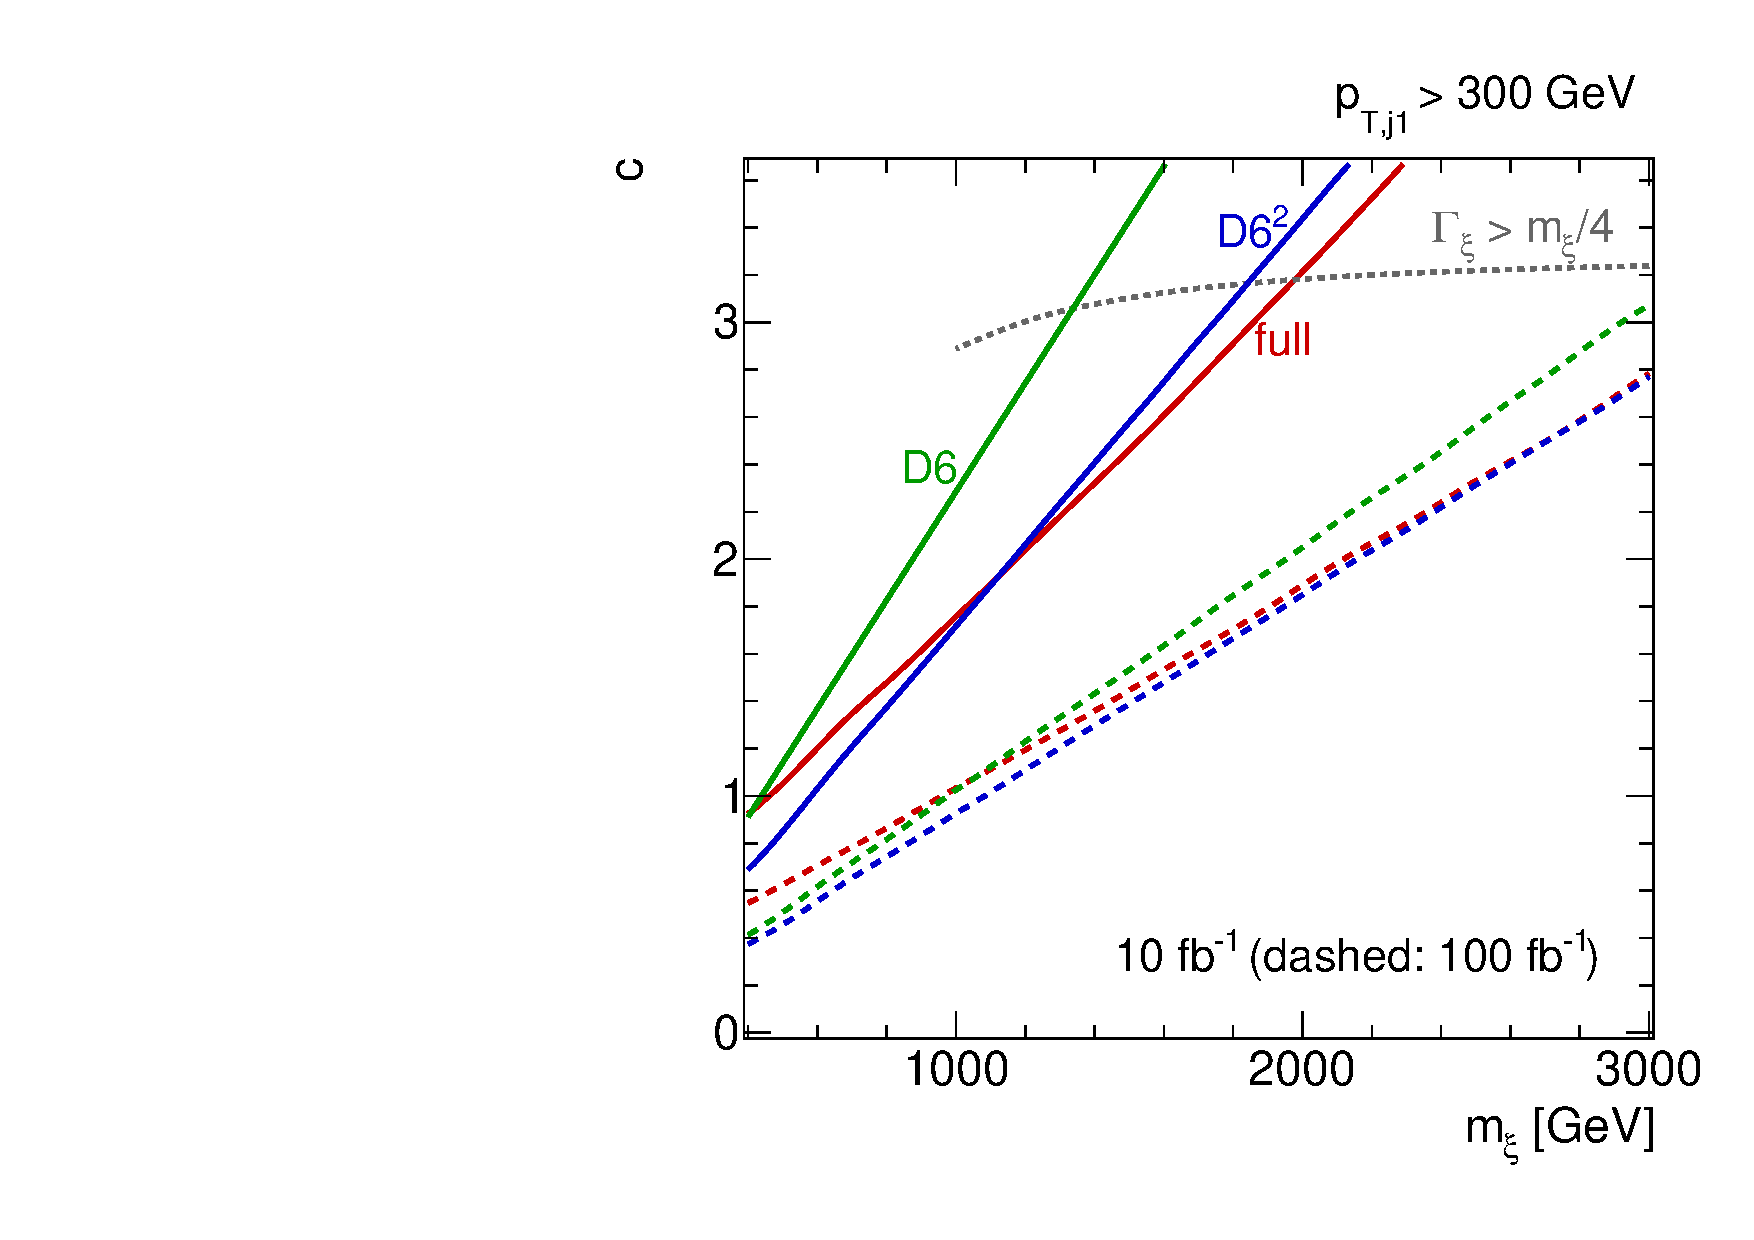
\includegraphics[width=0.43\textwidth]{fig/validity/WBF_limits_300.pdf} 
  \caption{Expected limits on a two-dimensional slice of the vector
    triplet parameter space. We show the analysis based on the event
    numbers in $150~\gev < p_{T,j_1} < 300~\gev$ (left) and based on
    the tail $p_{T,j_1} > 300$~GeV.}
  \label{fig:validity_limits}
\end{figure}
%------------------------------------------------------------


In the middle panels of \autoref{fig:validity_squared_WBF} we see that indeed
the $p_{T,h}$ distribution looks almost identical to $p_{T,j_1}$. Both
of them can be traced back to the unobservable virtualities of the
weak bosons. Due to the preferred collinear direction of the
quark-vector splittings, the $W$-mediated and $Z$-mediated diagrams
populate very different parton-level phase-space regions, with
basically no interference between them.  We can thus define the
virtuality variable~\cite{gino,polarized_ww}
%
\begin{align}
  q =
  \begin{cases}
    \max\left(   \sqrt{ | (p_{u'} - p_{d})^2 | } \, , \, \sqrt{ | (p_{d'} - p_{u})^2 | }  \right) & \text{for $W$-like phase-space points,} \\
    \max\left(   \sqrt{ | (p_{u'} - p_{u})^2 | } \, , \, \sqrt{ | (p_{d'} - p_{d})^2 | }  \right)  & \text{for $Z$-like phase-space points,}
  \end{cases}
  \label{eq:validity_virt}
\end{align}
%
with the distribution shown in the bottom panels of
\autoref{fig:validity_squared_WBF}. Comparing it to $p_{T,h}$ and $p_{T,j_1}$ we see
essentially the same behaviour.  The strong correlation of $q$ with
the observable transverse momenta of the leading tagging jet and the
Higgs is explicitly shown in \autoref{fig:validity_virt_corr}.

Finally, we compare expected exclusion limits on the vector triplet in
the absence of a signal, based on the full model vs the dimension-six
approach.  For the process shown in Equation\;\eqref{eq:validity_def_wbf} we
multiply the cross sections with a branching ratio
$\br(h \to 2\ell 2\nu) \approx 0.01$.  We disregard non-Higgs
backgrounds as well as parton-shower or detector effects.  We then
count events in two high-energy bins of the $p_{T,j_1}$ distributions,
defining a parameter point to be excluded if $S/\sqrt{S+B} > 2$.
While this statistical analysis is not designed to be realistic, it
illustrates how the validity of our dimension-six approach affects
possible limits.  For our limit setting procedure we choose a
two-dimensional plane defined by $m_\xi$ versus a universal coupling
rescaling $c$,
%
\begin{align}
  g_V = 1 \; , \qqquad 
  c_H = c \; , \qqquad 
  c_F = \frac {g_V^2}{2g^2} \, c \; , \qqquad 
  c_{HHVV} = c^2 \; .
\end{align}
%
This reduces the list of generated dimension-six operators to
%
\begin{align}
  f_{WW} = f_{BW} = \frac {c^2} {2g^2} \qquad \text{and} \qquad  f_W = - \frac {c^2} {g^2} \,,
\end{align}
%
and all dimension-six deviations scale like $c^2/m_\xi^2$. To avoid
effects from strongly interacting theories we limit our analysis to
$\Gamma_{\xi}/m_{\xi} < 1/4$.

In the left panel of \autoref{fig:validity_limits} we see that based on event
numbers in the range $150~\text{GeV} < p_{T,j_1} < 300~\text{GeV}$,
the dimension-six approximation with the squared terms gives the
same limits as the full model, as long as we ensure that the new
resonance remains narrow.  In the high-energy tail
$p_{T,j_1} > 300$~GeV including the squared terms also improves the validity of
the dimension-six approach, but it only leads to identical limits for
large $m_\xi$, combined with strong couplings. Indeed, limiting the
momentum transfer of events for example through an upper limit on
$p_{T,j}$ is well known to reduce the dependence on model
assumptions~\cite{spins1,spins2}.

Just as for the $Vh$ production process, at least as long as the event
numbers remain small the square of the dimension-six operators always
improves the agreement with the full theory in weak boson fusion. With
improved statistics the differences become smaller and ultimately
negligible, and the question of whether the squared dimension-six
amplitudes should be taken into account is rendered irrelevant.





%%%%%%%%%%%%%%%%%%%%%%%%%%%%%%%%%%%%%%%%%%%%%%%%%%%%%%%%%%%%
\subsection{Realistic tagging jets}
%%%%%%%%%%%%%%%%%%%%%%%%%%%%%%%%%%%%%%%%%%%%%%%%%%%%%%%%%%%%

%------------------------------------------------------------
\begin{figure}[t]
  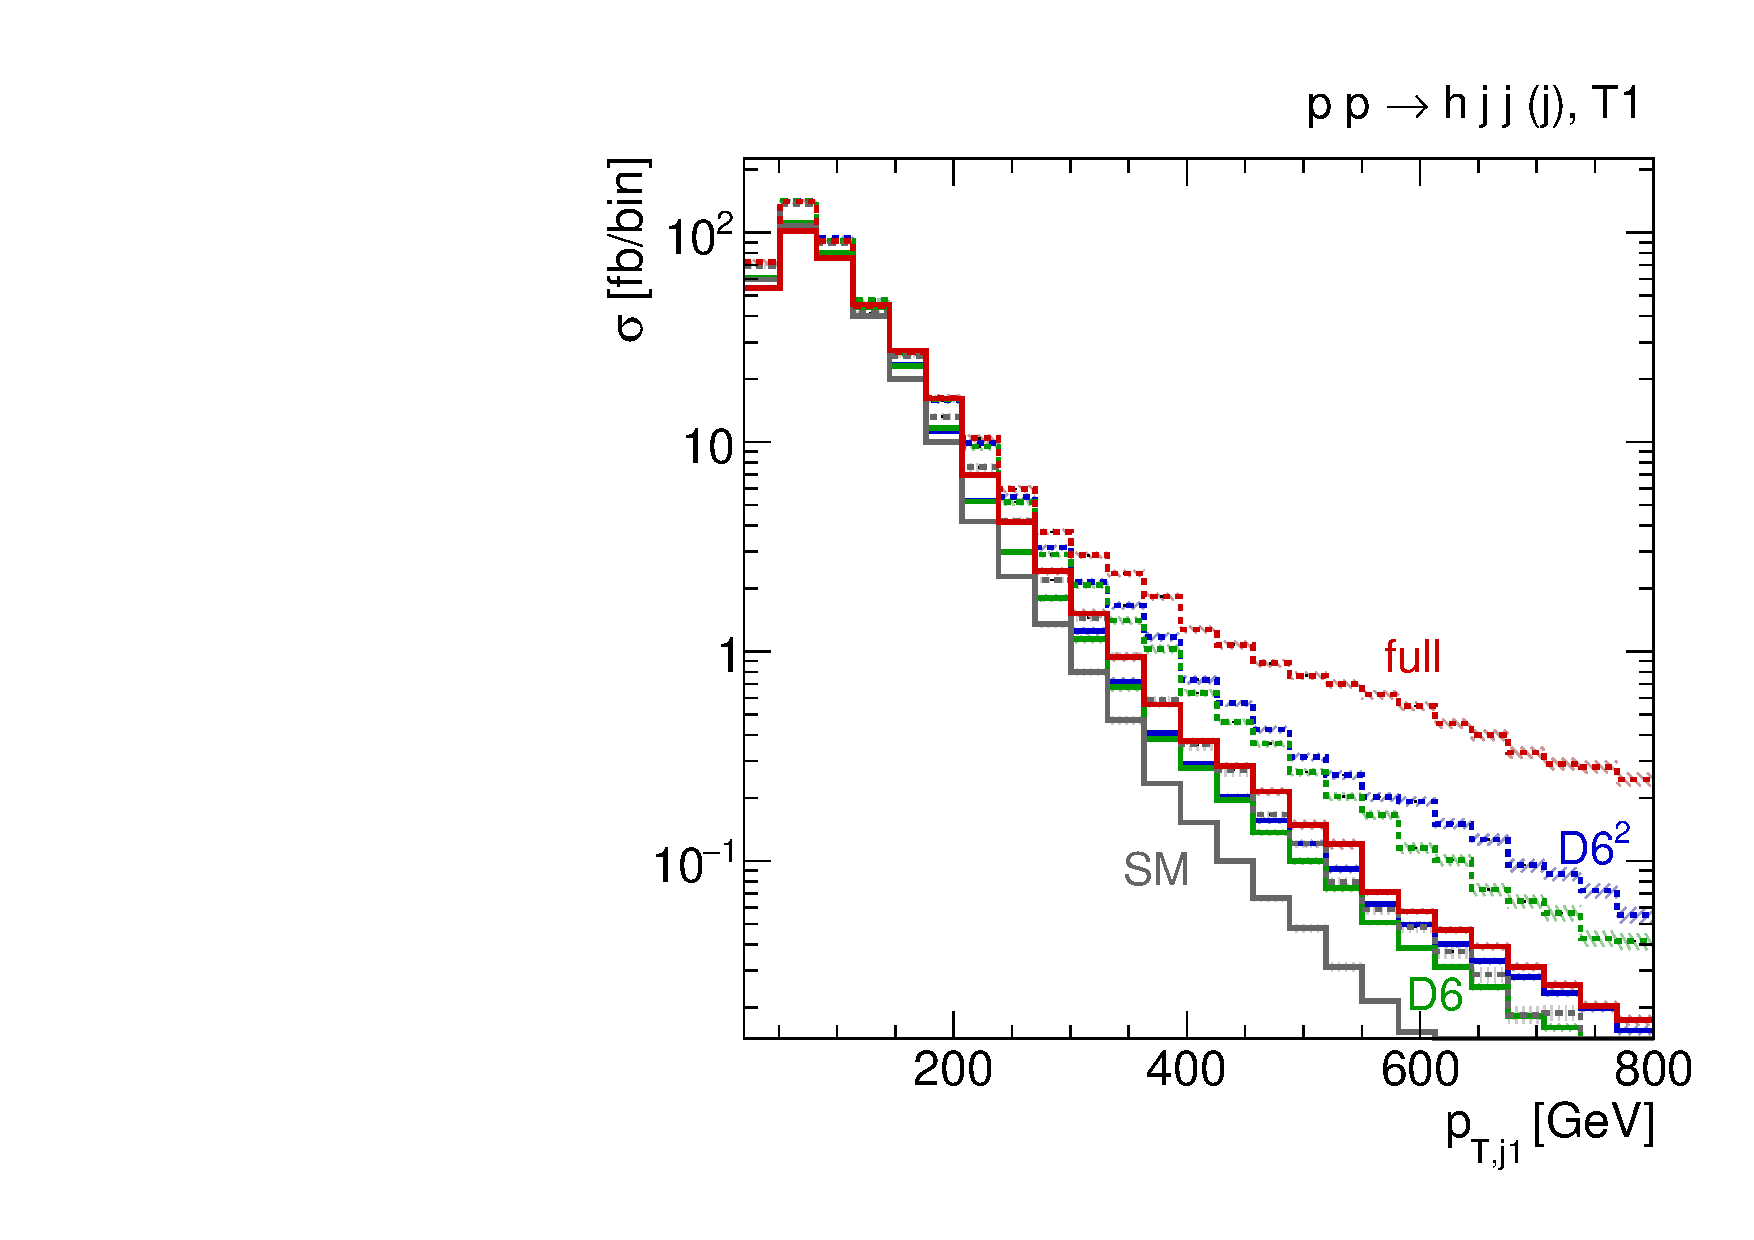
\includegraphics[width=0.43\textwidth]{fig/validity/WBF_realistic_T1_j1pt.pdf}
  \hspace*{0.05\textwidth}
  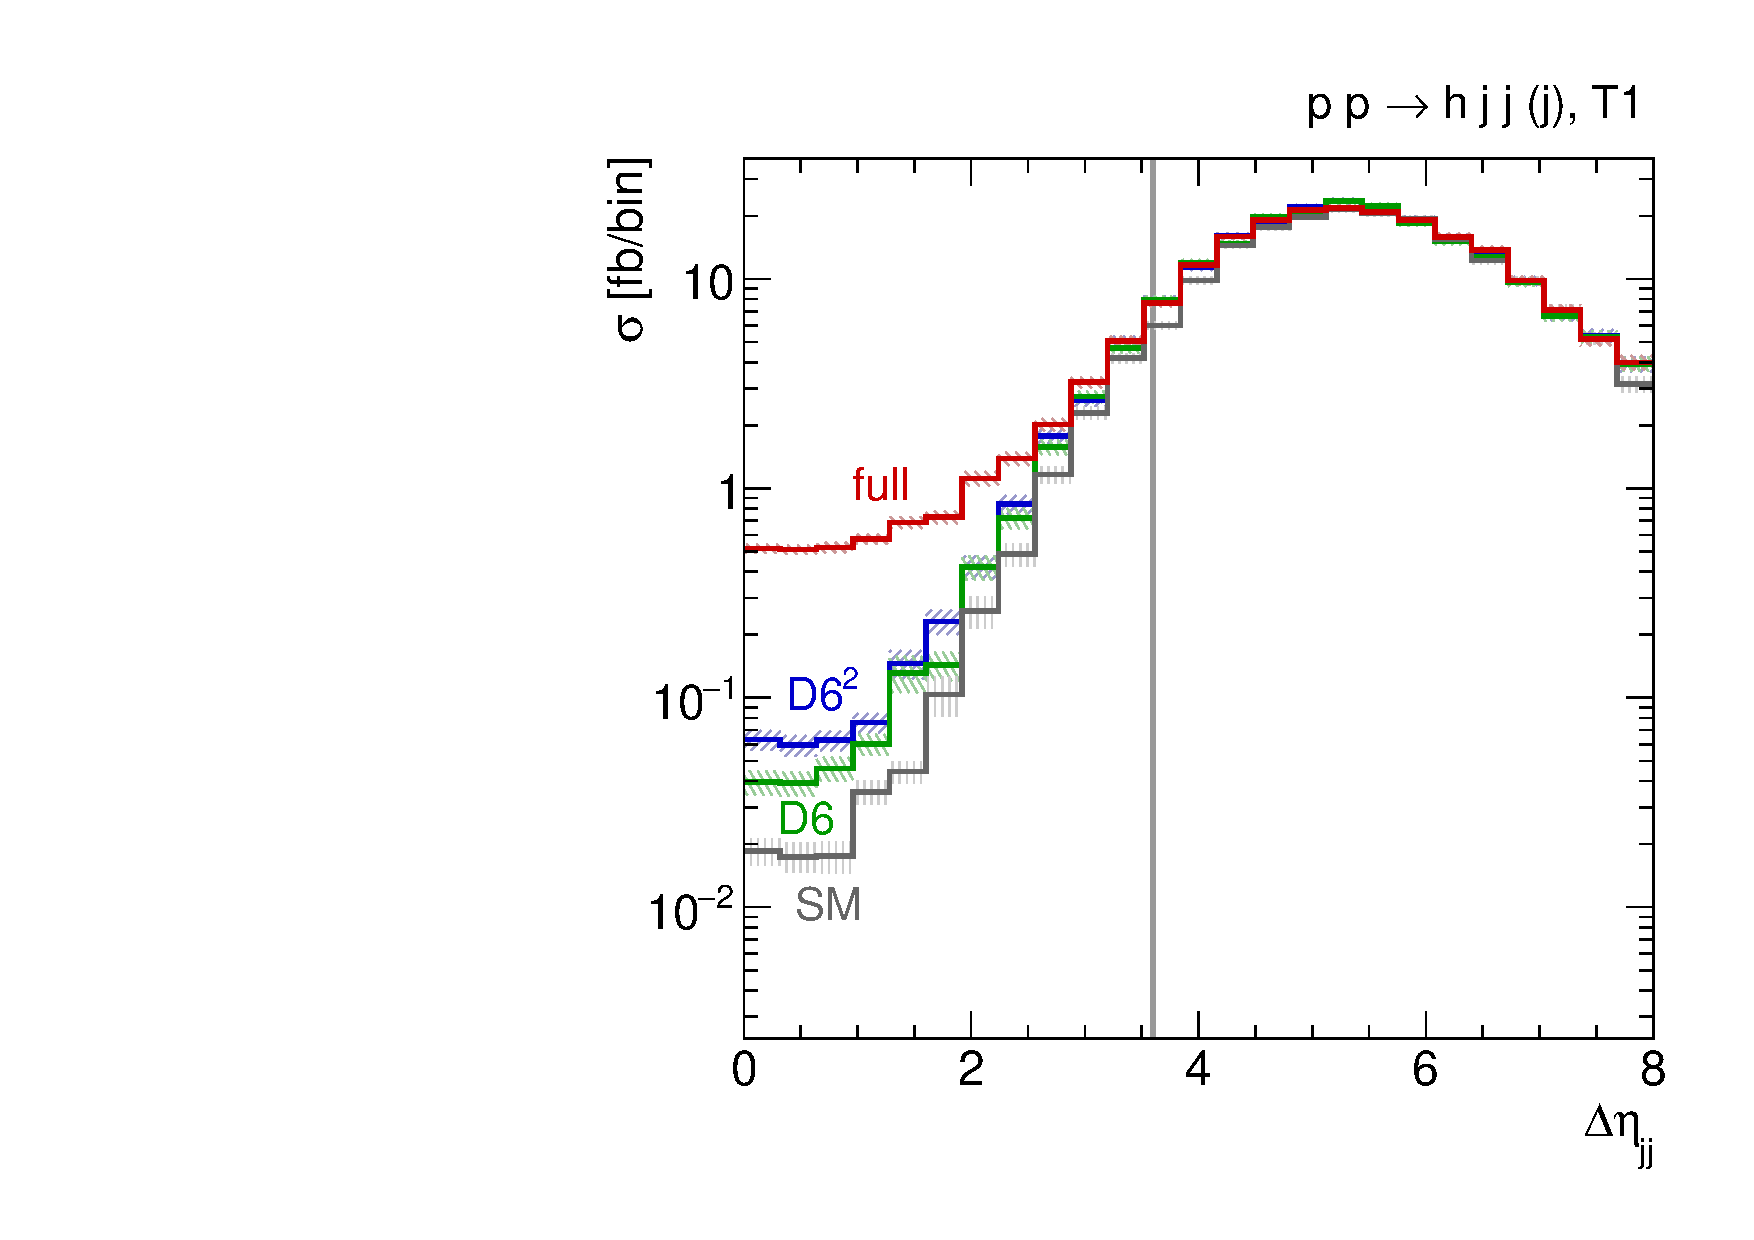
\includegraphics[width=0.43\textwidth]{fig/validity/WBF_realistic_T1_deltaEtaJJ.pdf}
  \caption{WBF distribution at hadron level. Left: $p_{T,j_1}$
    distribution based on the full process, the dashed lines show the
    distributions based on WBF diagrams only and without a
    $\Delta \eta_{jj}$ cut. Right: $\Delta \eta_{jj}$ based on WBF
    diagrams only, the vertical line marks the standard WBF cut
    following Equation\;\eqref{eq:validity_wbf_cuts}.}
  \label{fig:validity_realistic_jets}
\end{figure}
%------------------------------------------------------------

Before we attempt to further improve the description of the full vector
triplet model for example in the benchmark point T1, we briefly test
if the parton-level effects described above survive a realistic environment.
We add a parton shower and jet reconstruction now for the full
process
%
\begin{align}
  p p \to h \; j j \, (+j) \; ,
\end{align}
%
simulated in \toolfont{MadGraph}~\cite{madgraph}.  Parton showering is
performed by \toolfont{PYTHIA6}~\cite{pythia} using the $k_T$-jet MLM
matching scheme~\cite{mlm} with a minimum $k_T$ jet measure between
partons of \toolfont{xqcut}=20~GeV. \toolfont{Fastjet}~\cite{fastjet}
is used to construct jets based on the $k_T$ algorithm with $R = 0.4$. We do not
include a Higgs decay because we are only interested in
production-side kinematics.  The standard WBF cuts then are
%
\begin{align}
  p_{T,j} > 20~\gev \,, \qqquad 
  m_{jj} > 500~\gev \,, \qqquad 
  \Delta \eta_{jj}~>~3.6
\label{eq:validity_wbf_cuts}
\end{align}
%
on the two hardest jets. We veto additional jets with
$p_{T,j} > 20$~GeV between these two tagging jets.  To analyse the
effects of the $\Delta \eta_{jj}$ cut~\cite{spins2}, we generate
additional samples explicitly excluding Higgs-strahlung diagrams, in
spite of the fact that it might break gauge invariance.

In \autoref{fig:validity_realistic_jets} we show that the distributions are
generally robust under parton shower and jet reconstruction, but two
complications arise.  First, on-shell $\xi$ production contributes to
this process and is not entirely removed by the WBF cuts in
Equation\;\eqref{eq:validity_wbf_cuts}, leading to visible differences between the
full and effective model already at low momenta. Such a resonance peak
would be easy to identify experimentally and does not present a major
problem for the dimension-six approximation.

Second, the tension between the full model and the dimension-six
approximation at large momenta now remains below $10~\%$.  This means
that the $\Delta \eta_{jj}$ cut not only removes large contributions
from Higgs-strahlung--like diagrams, it also gets rid of phase-space
regions where the full model and the dimension-six description differ
the most.  At the same time, the $\Delta \eta_{jj}$ removes some of
its well-known discrimination power for new physics effects versus the
Standard Model~\cite{spins2}.




%%%%%%%%%%%%%%%%%%%%%%%%%%%%%%%%%%%%%%%%%%%%%%%%%%%%%%%%%%%%
\subsection{Towards a simplified model}
\label{sec:validity_simplified}
%%%%%%%%%%%%%%%%%%%%%%%%%%%%%%%%%%%%%%%%%%%%%%%%%%%%%%%%%%%%

%------------------------------------------------------------
\begin{figure}[t]
  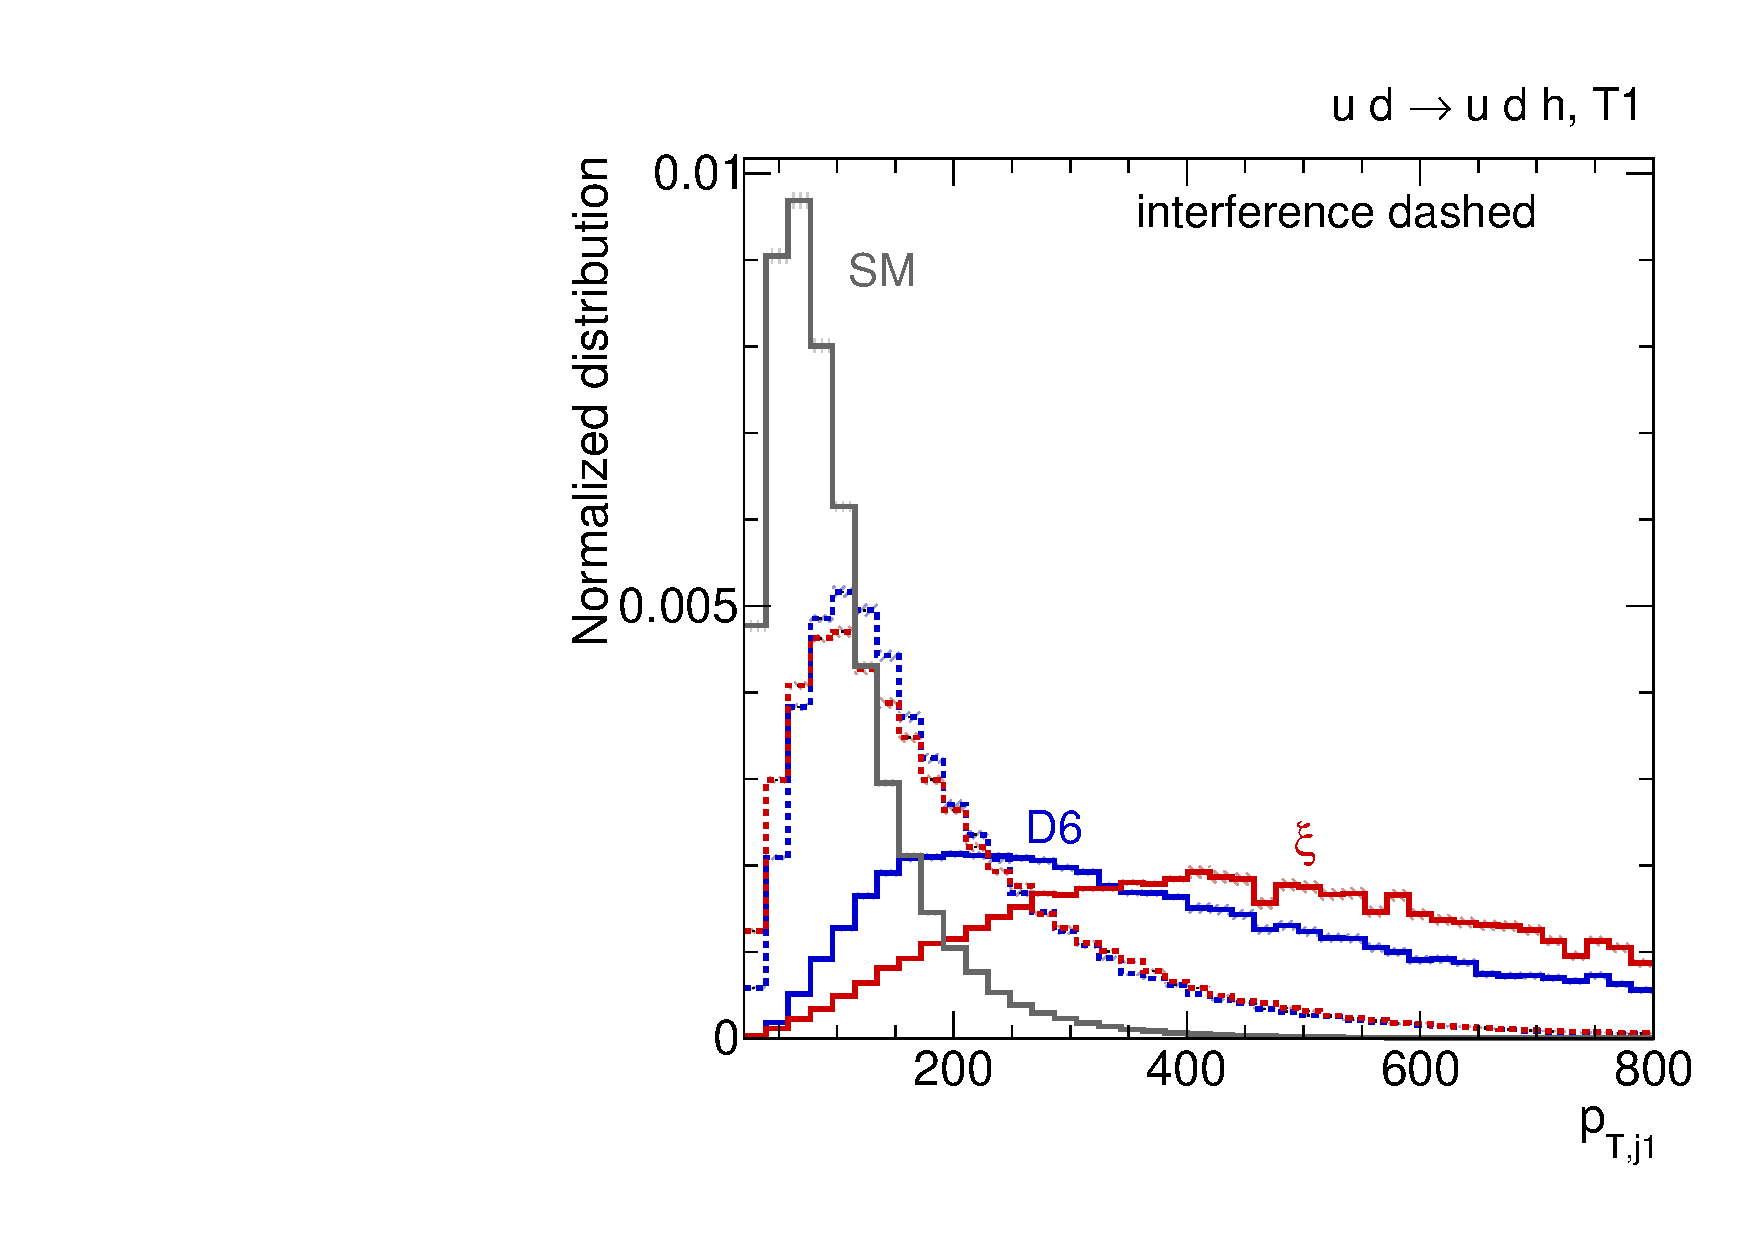
\includegraphics[width=0.43\textwidth]{fig/validity/WBF_separate_T1_j1pt.pdf} 
  \hspace*{0.05\textwidth}
  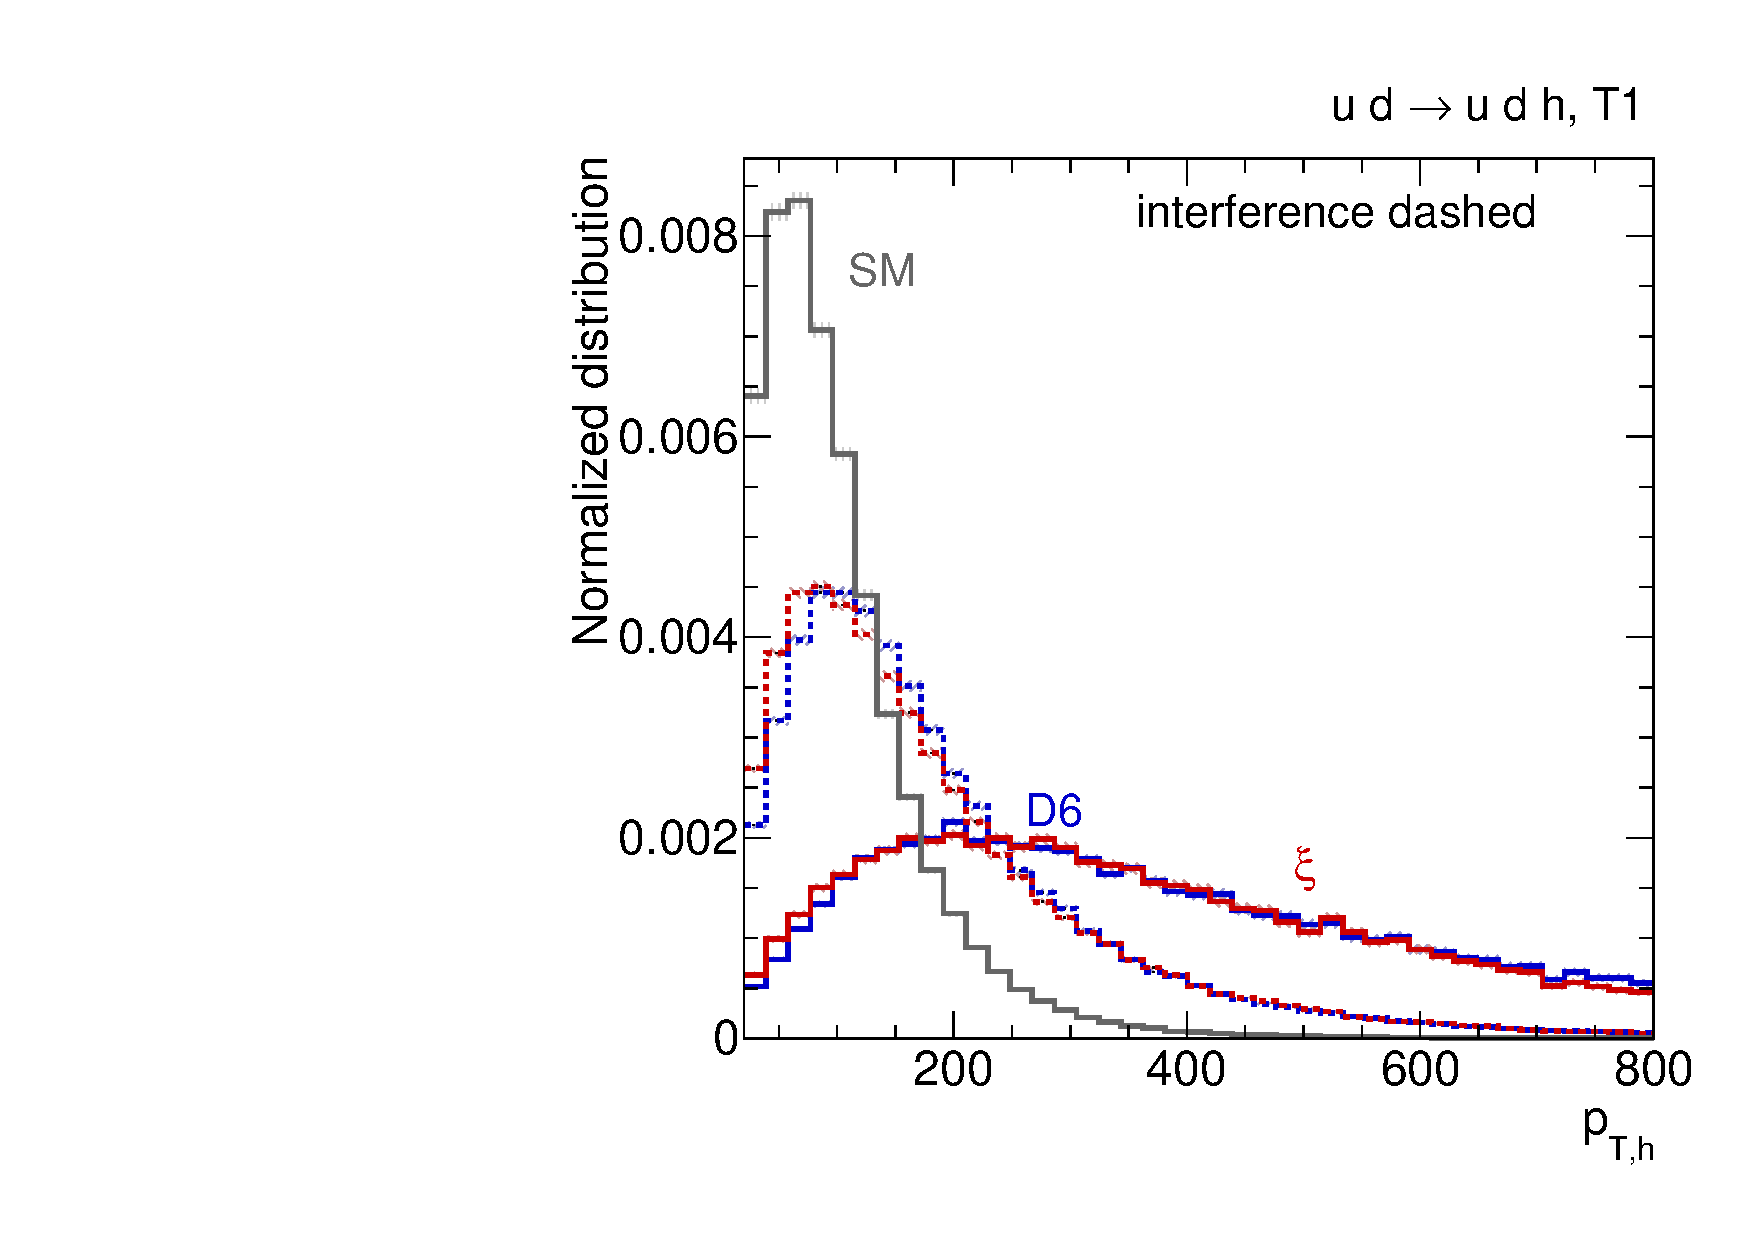
\includegraphics[width=0.43\textwidth]{fig/validity/WBF_separate_T1_Hpt.pdf}\\
  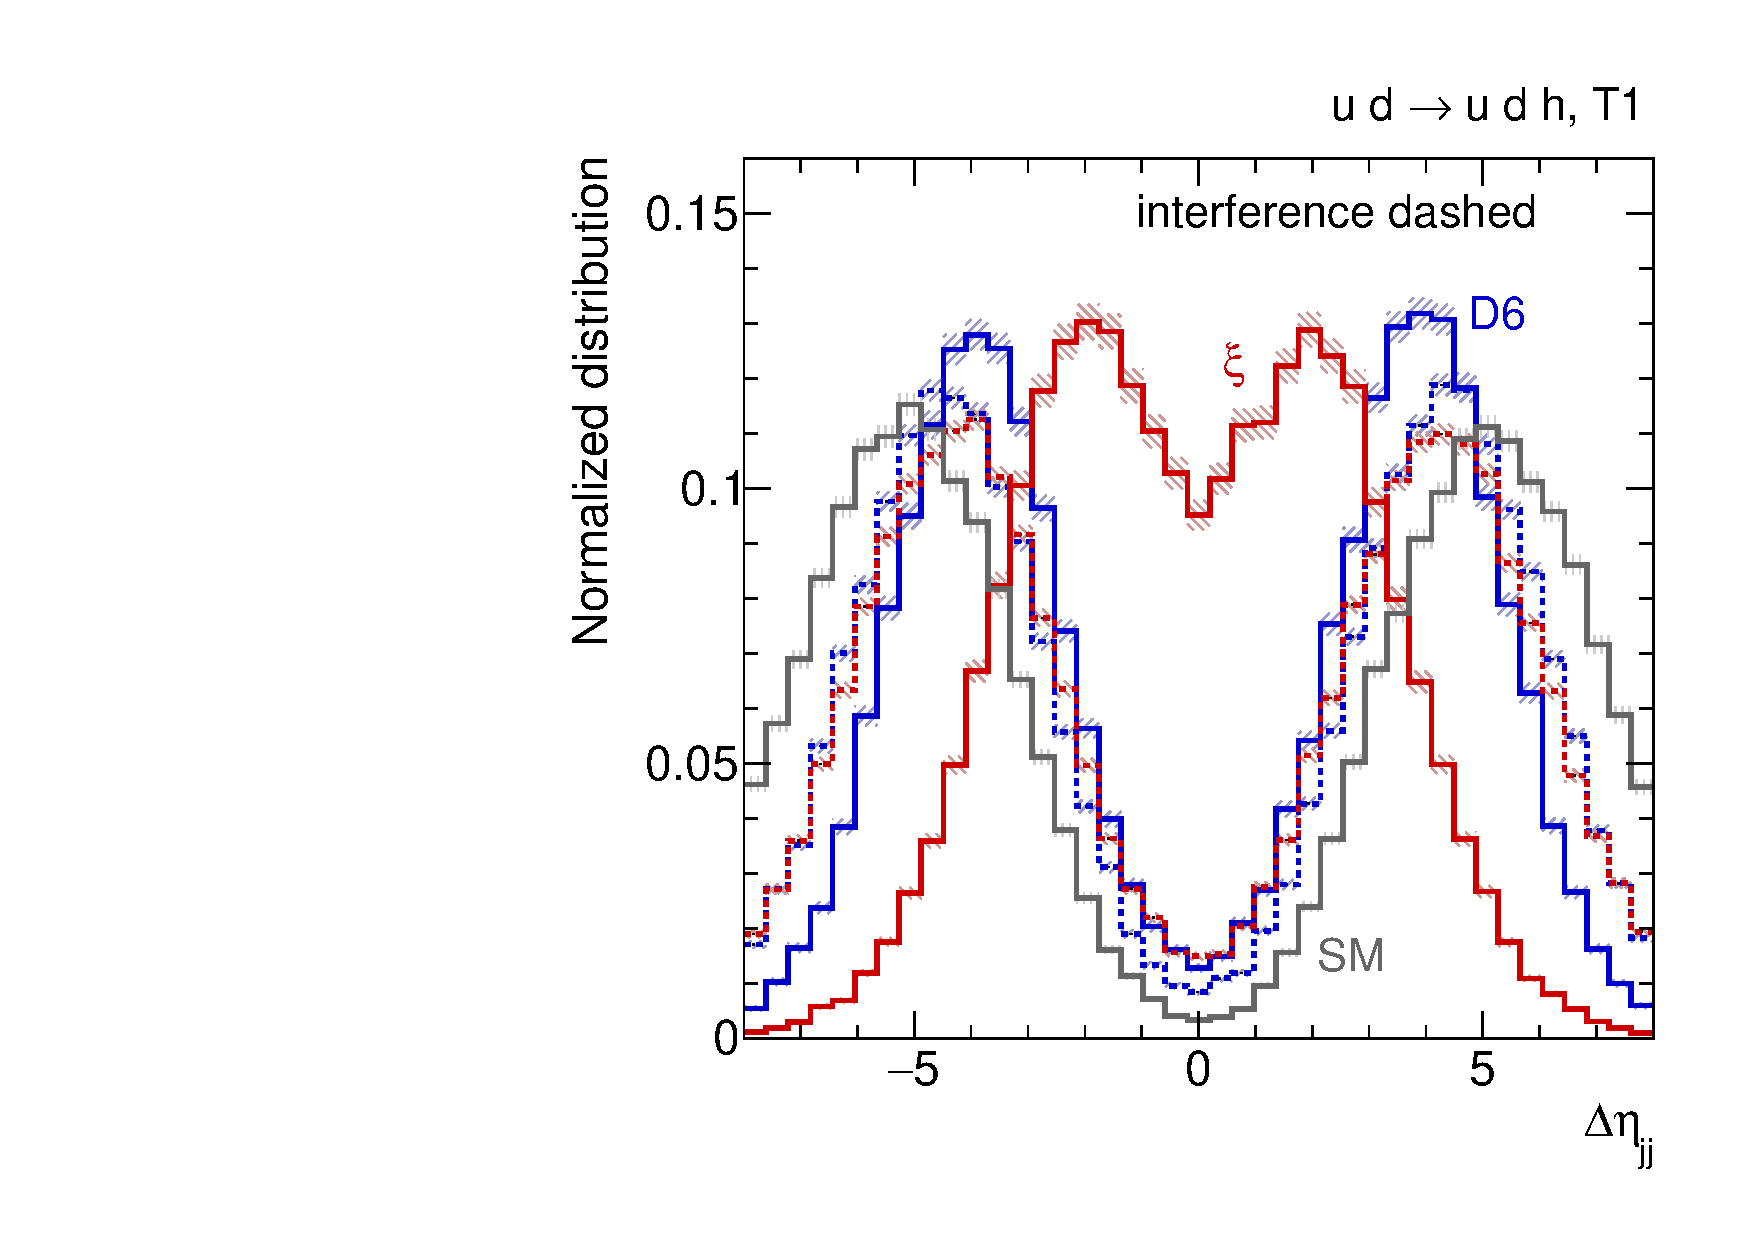
\includegraphics[width=0.43\textwidth]{fig/validity/WBF_separate_T1_deltaEtaJJ.pdf} 
  \hspace*{0.05\textwidth}
  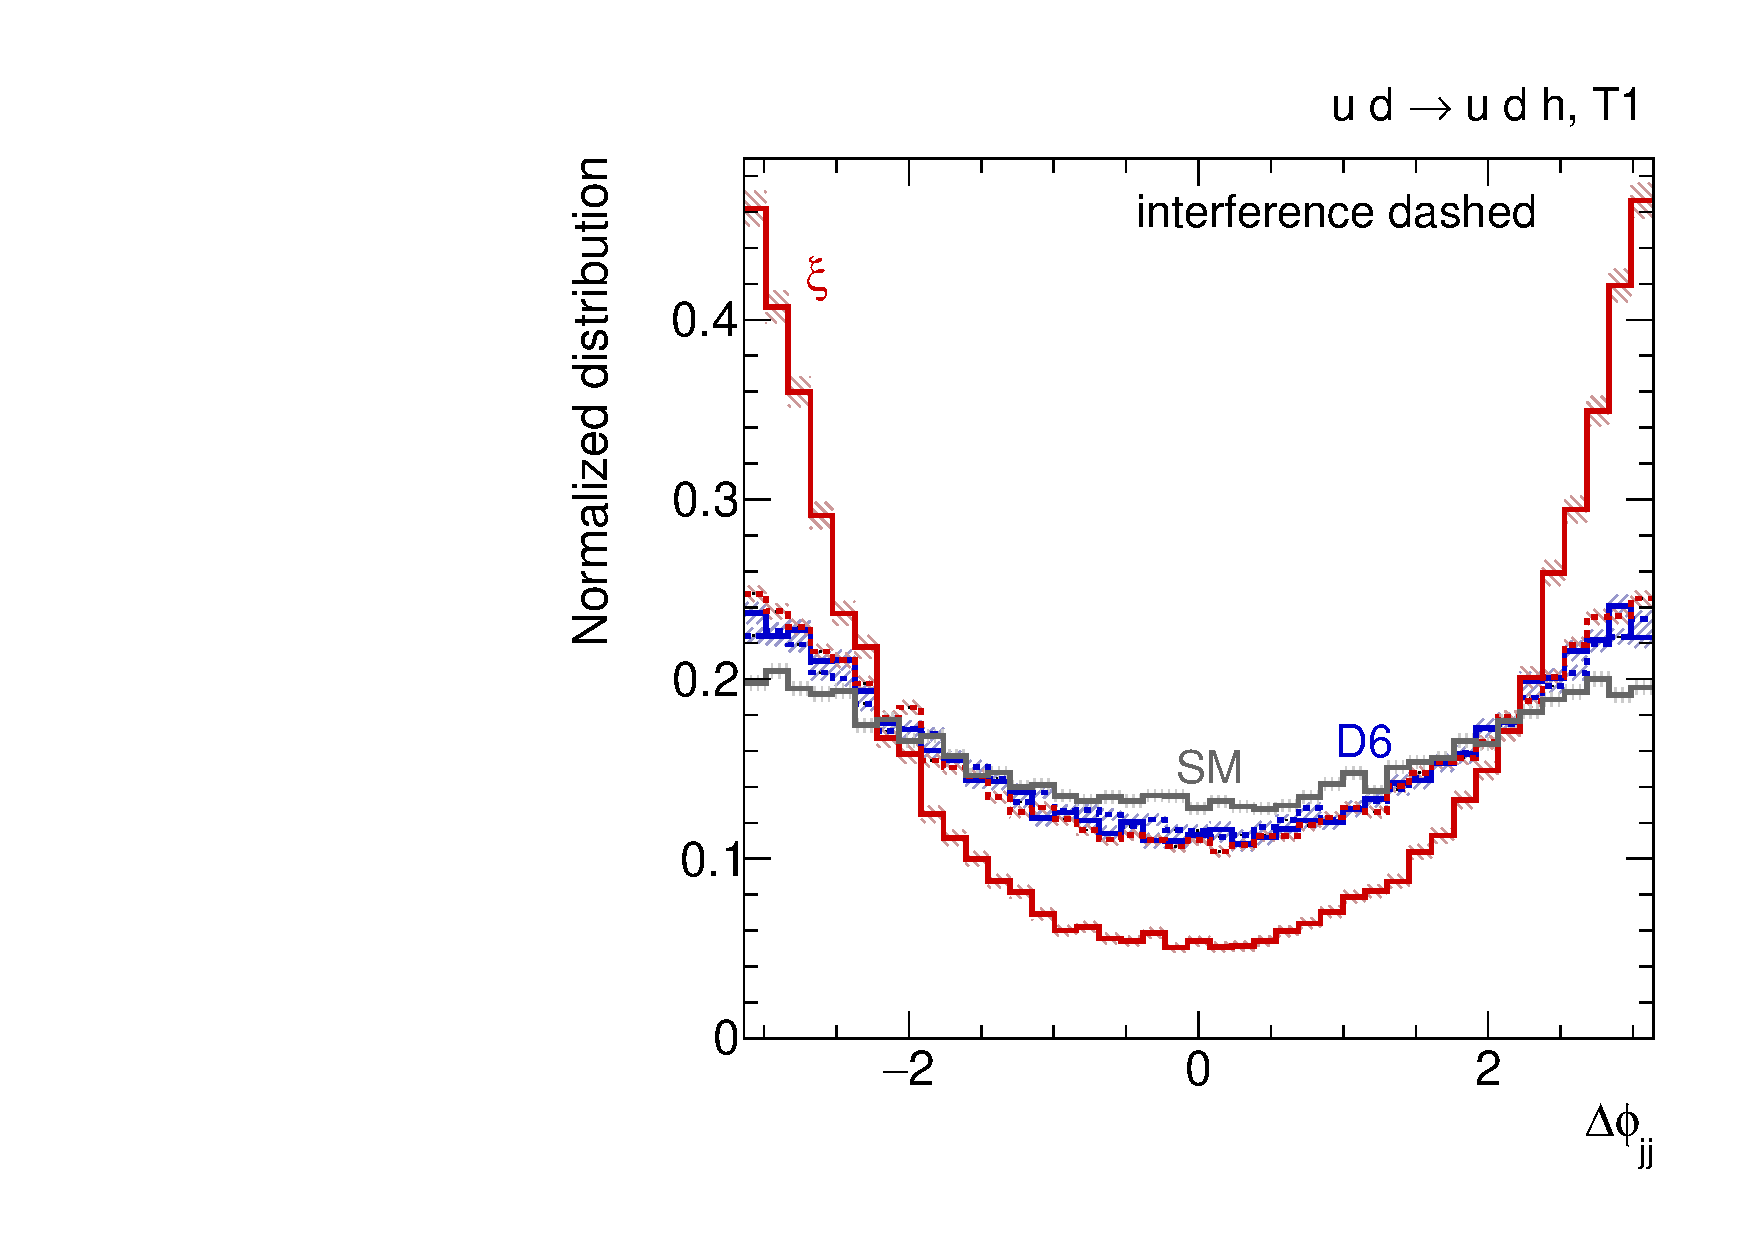
\includegraphics[width=0.43\textwidth]{fig/validity/WBF_separate_T1_deltaPhiJJ.pdf}
  \caption{Normalised WBF distributions of the tagging jets. We separate
    the squared new-physics amplitudes, shown as solid lines, from the
    interference with the SM-like diagrams (dashed).}
  \label{fig:validity_squared_separate}
\end{figure}
%------------------------------------------------------------

In the first part of the paper we have shown where in phase space a
dimension-six description of LHC observables breaks down, both for $Vh$
production and for weak boson fusion. For $Vh$ production with its
simple $2 \to 2$ kinematics problems are clearly linked to a possible
$s$-channel resonance, as seen in Equation\;\eqref{eq:validity_breakdown_vh}.  For
weak boson fusion there appears no resonance, but the result of
Equation\;\eqref{eq:validity_breakdown_wbf} suggests that the new states in the
$t$-channel have a similar effect.  In \autoref{fig:validity_squared_separate}
we show different tagging jet distributions, separating the Feynman
diagrams including the heavy $\xi$ states. In particular for the
critical $p_{T,j_1}$ distribution, the $\Delta \eta_{jj}$
distribution, and the $\Delta \phi_{jj}$ distribution these diagrams
are only very poorly described by the dimension-six approach. In
practice this is not a problem because these contributions are
strongly suppressed by the heavy mass $m_\xi$, but it poses the
question how we can improve the agreement. The obvious solution to
these problems in the $s$-channel of $Vh$ production and in the
$t$-channel of weak boson fusion is a simplified
model~\cite{simp,simp_higgs}. A new vector field mixing with the weak
bosons as described by the Lagrangian shown in
Equation\;\eqref{eq:validity_lag-vectortriplet} is such a simplified model, but its
structure is still relatively complex. Obviously, an additional heavy
scalar with mass around $m_\xi$ and the appropriate couplings will
improve the $2 \to 2$ kinematics for $Vh$ production. The question we
want to study in this section is if such a scalar can also improve the
weak boson fusion kinematics.



%%%%%%%%%%%%%%%%%%%%%%%%%%%%%%%%%%%%%%%%%%%%%%%%%%%%%%%%%%%%
\subsubsection*{A pseudo-scalar as a simplified vector}
%%%%%%%%%%%%%%%%%%%%%%%%%%%%%%%%%%%%%%%%%%%%%%%%%%%%%%%%%%%%

The simplest simplified model we can write down includes one new
massive scalar $S$ with a Higgs portal and a Yukawa coupling. 
However, a scalar state will not interfere with the Standard Model
diagrams. In analogy to the CP properties of the Goldstone mode
contributing to the massive $Z$ boson we define our simplified model
with a pseudo-scalar state as
%
\begin{align}
\mathcal{L} \supset 
  \frac{1}{2} (\partial_\mu S)^2 
- \frac{m_S}{2} S^2 
+ \sum_\text{fermions} g_F \; S \overline{F} \gamma_5 F 
+ g_S \; S^2 \phi^\dagger \phi \,.
  \label{eq:validity_simplified_model}
\end{align}

%------------------------------------------------------------
\begin{figure}[t]
  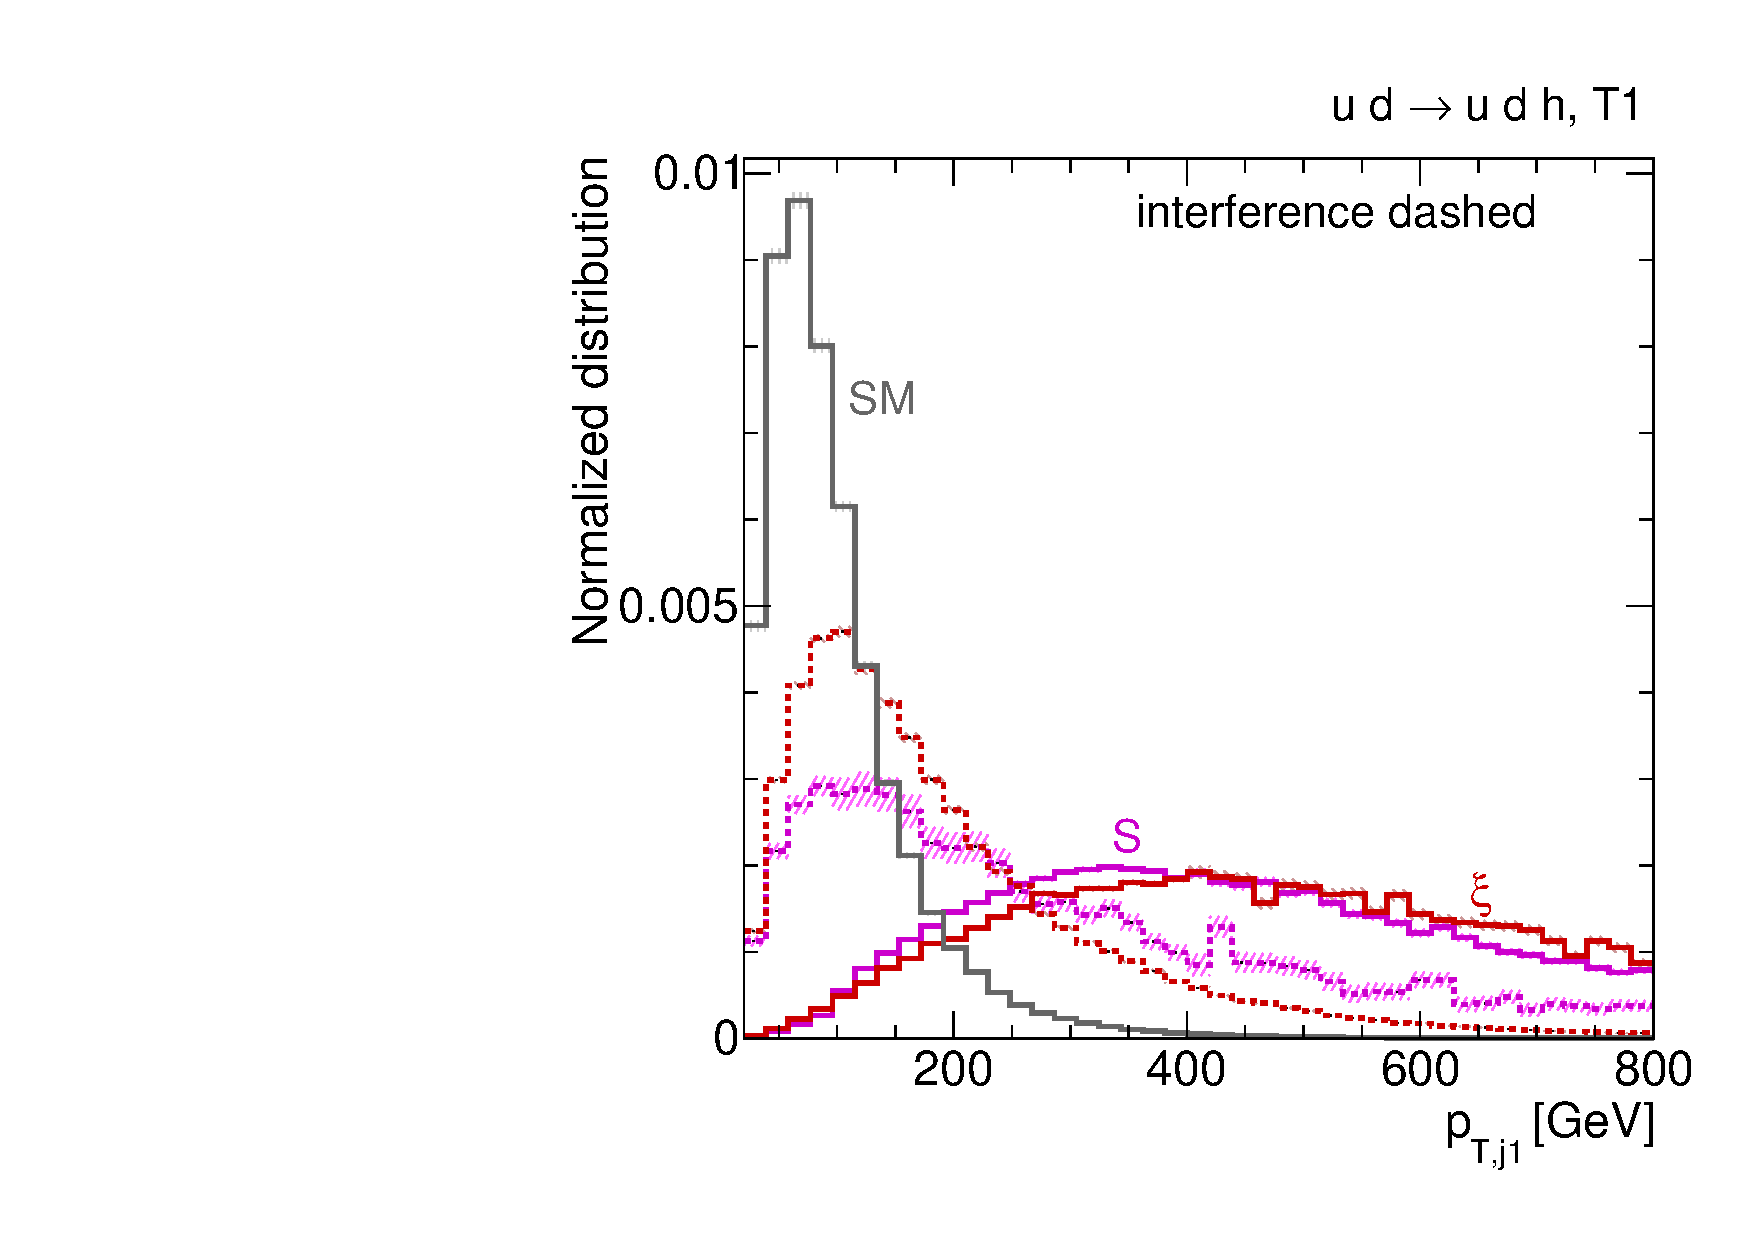
\includegraphics[width=0.43\textwidth]{fig/validity/WBF_simplified_j1pt.pdf}
  \hspace*{0.05\textwidth}
  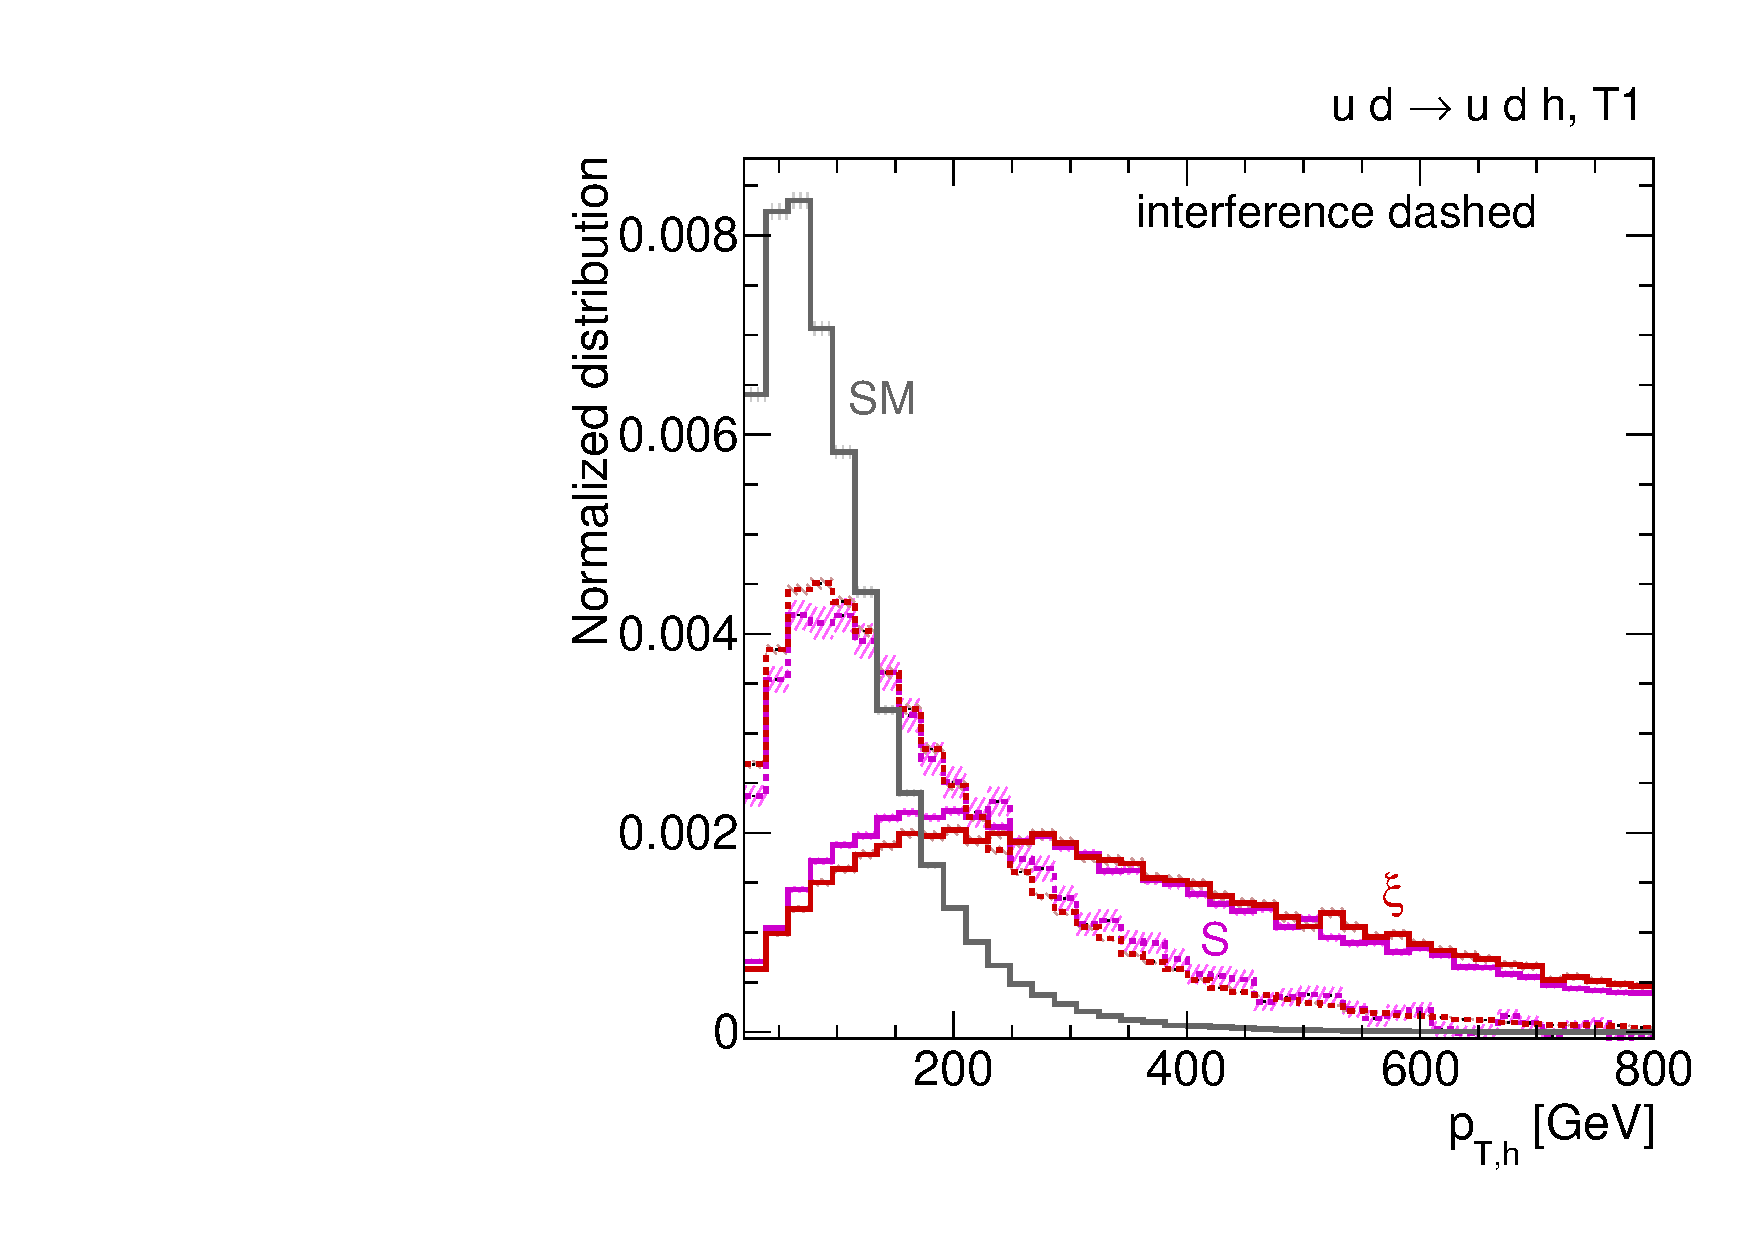
\includegraphics[width=0.43\textwidth]{fig/validity/WBF_simplified_Hpt.pdf} \\
  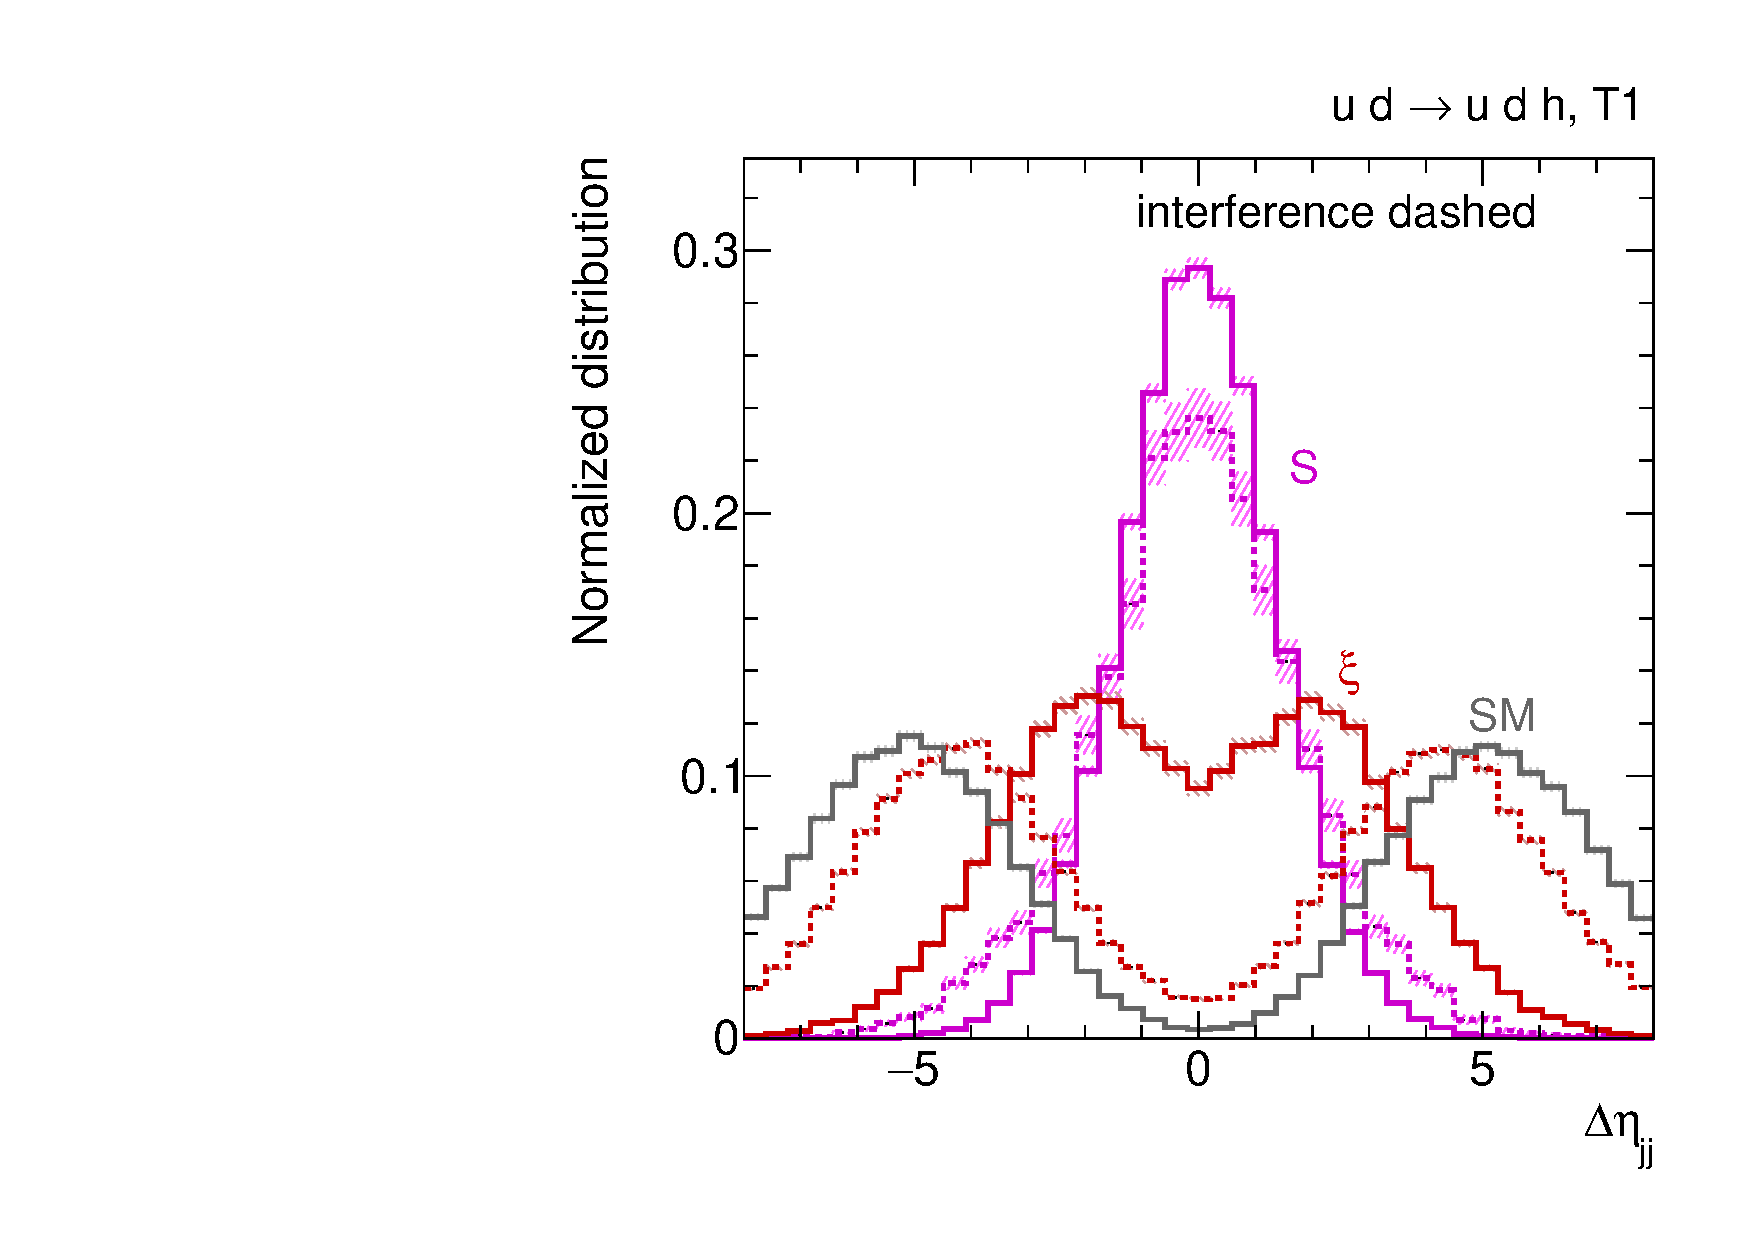
\includegraphics[width=0.43\textwidth]{fig/validity/WBF_simplified_deltaEtaJJ.pdf}
  \hspace*{0.05\textwidth}
  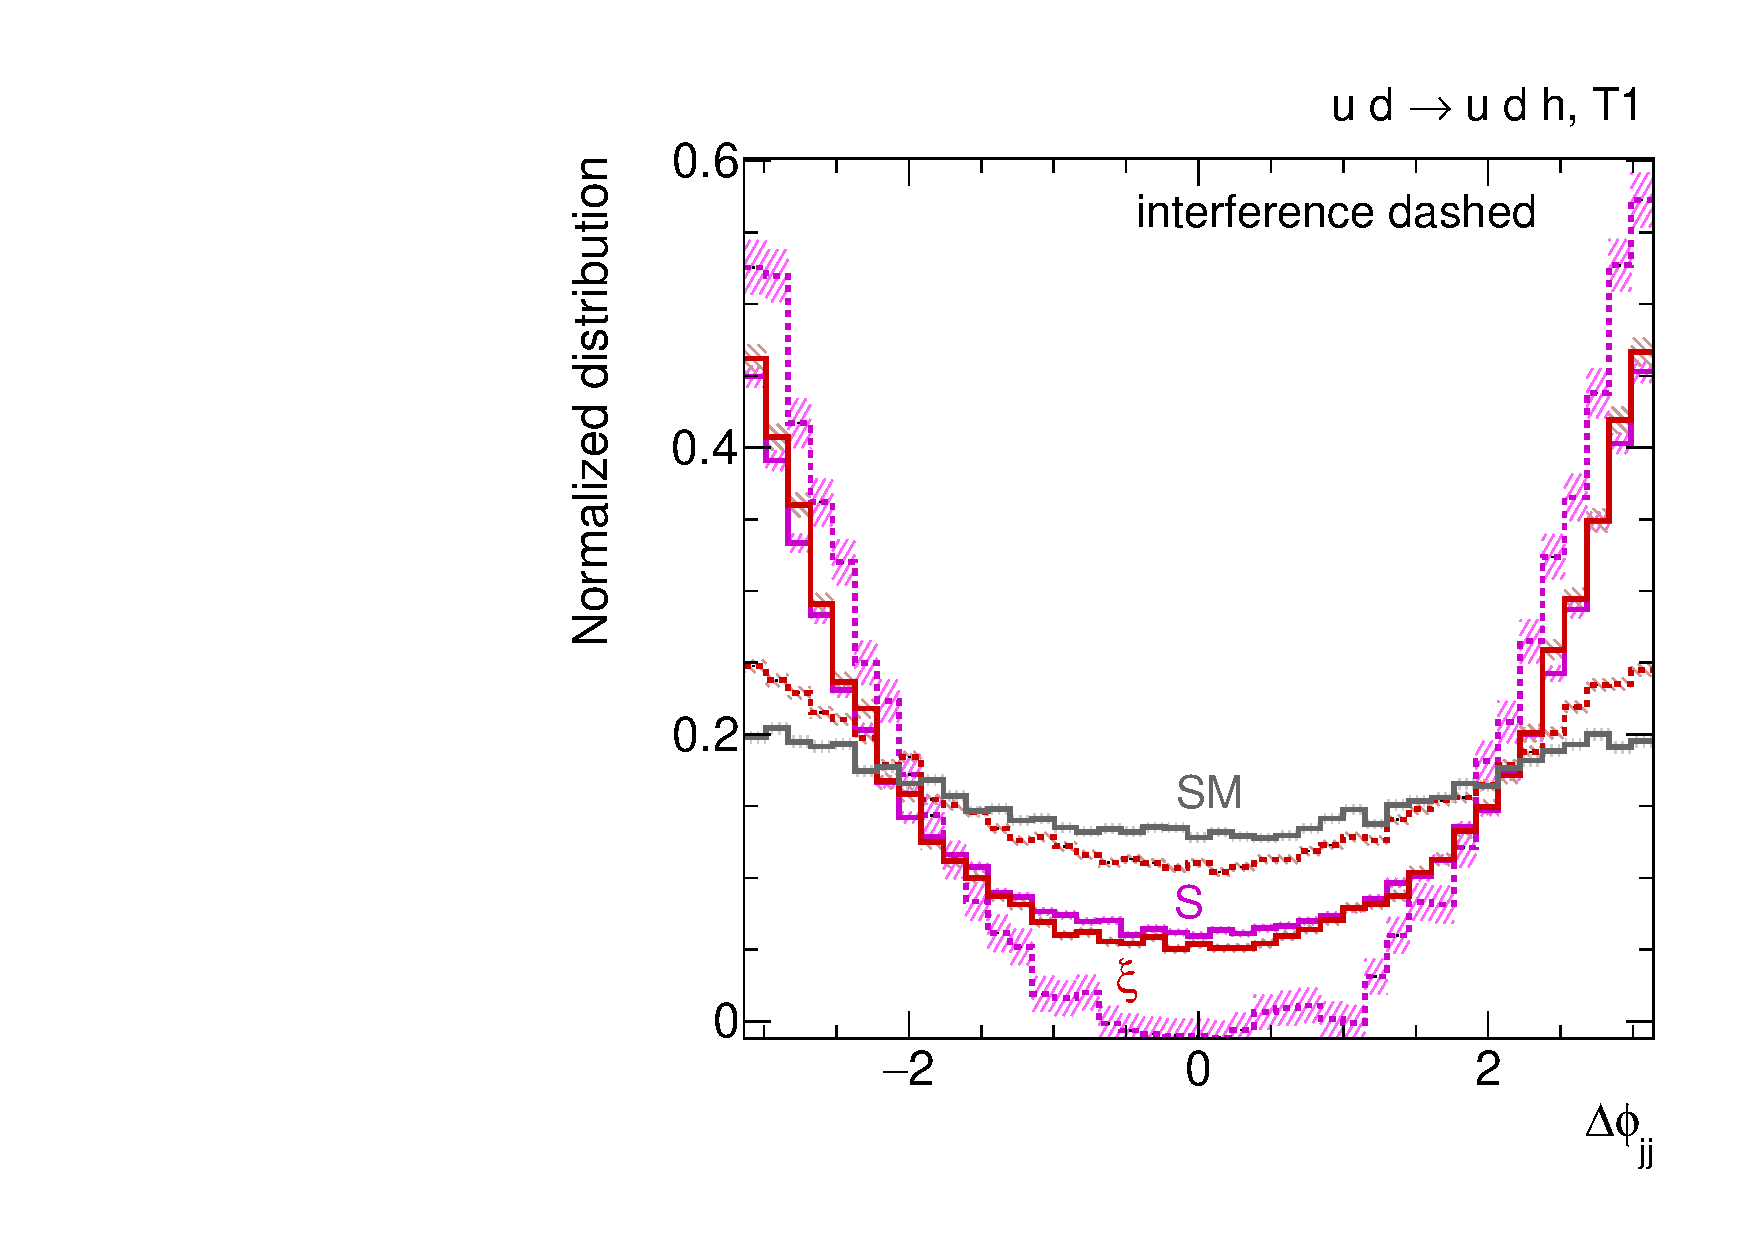
\includegraphics[width=0.43\textwidth]{fig/validity/WBF_simplified_deltaPhiJJ.pdf}
  \caption{Normalised WBF distributions for a scalar simplified model
    defined in Equation\;\eqref{eq:validity_simplified_model} vs the vector triplet
    benchmark.}
  \label{fig:validity_simplified}
\end{figure}
%------------------------------------------------------------

In \autoref{fig:validity_simplified} we show the same WBF distributions as in
\autoref{fig:validity_squared_separate}, but including the simplified scalar
model. For the $p_{T,j}$ distribution the squared new-physics
amplitudes in the full vector model and the simplified scalar model
indeed agree well, improving upon the dimension-six description which
breaks down in this distribution.  However, the interference term with
the Standard Model, which is numerically dominant for most of the
distribution and well described in the dimension-six model, poses a
problem.  The $\Delta \eta_{jj}$ distributions show even poorer
agreement: the spin-1 amplitudes of the Standard Model and the vector
triplet have similar phase-space distributions and give two forward
tagging jets, while the scalar mediator favours central
jets~\cite{spins2}.  The $\Delta \phi_{jj}$ distribution, known to be
sensitive to the tensor structure of the hard $VVh$
interaction~\cite{delta_phi}, exposes similar differences between the
full and simplified model.  Altogether, our simplified scalar model
with its very different $VVh$ interaction structure does improve the
description in the region where the dimension-six approach breaks down,
but it fails to describe interference patterns and angular
correlations of the tagging jets.



%%%%%%%%%%%%%%%%%%%%%%%%%%%%%%%%%%%%%%%%%%%%%%%%%%%%%%%%%%%%
\subsubsection*{Splitting functions and equivalence theorem}
%%%%%%%%%%%%%%%%%%%%%%%%%%%%%%%%%%%%%%%%%%%%%%%%%%%%%%%%%%%%

We can understand this very different behaviour of the scalar
$t$-channel mediator as compared to the vector from the splitting
kernels in the collinear limit.  The matrix element squared for the
weak boson fusion process mediated by pseudo-scalars $S$ has the form
%
\begin{align}
 | \mathcal{M}(qq \to q'q'h) |^2 \propto 
  \frac{g_F^4 \;  t_1 t_2}{(t_1 - m_S^2)^2 \; (t_2 - m_S^2)^2} 
\stackrel{m_S \to 0}{\longrightarrow} \frac{\text{const}}{t_1 t_2} \; ,
\end{align}
%
where $t_1$ and $t_2$ denote the respective momentum flow through each
scalar propagator. For $m_S \to 0$ the Jacobians from the phase-space
integration cancel a possible collinear divergence, while for a light
vector boson a soft and a collinear divergence remains. Unlike in the
usual WBF process, the tagging jets in our simplified scalar model
will not be forward.  The reason for this difference in the
infrared is the (pseudo-)scalar coupling to quarks: since the scalar
carries no Lorentz index, a $q \to q S$ splitting will be expressed in
terms of the momentum combinations $(p_q p_q')$, $p_q^2 = m_q^2$, and
$p_q'^2 = m_q^2$. In the limit of massless quarks only the first term
remains as $t = 2 (p_q p_q')$.  This factor in the numerator cancels
the apparent divergence of the $t$-channel propagator.

Adding higher-dimensional couplings of the (pseudo-)scalar to
fermions, such as
%
\begin{align}
  \mathcal{L} \supset 
\sum_\text{fermions} \Biggl[  
  g_{F,2} S \overline{F} F 
+ g_{F,3} (\partial_\mu S) \overline{F} \gamma^\mu F
+ g_{F,4} S (\partial_\mu S) \overline{F} \gamma^\mu \gamma_5 F 
+ g_{F,5} S (\partial_\mu \partial_\nu S) \overline{F} [\gamma^\mu,\gamma^\nu] F
\Biggr] \; ,
\label{eq:validity_simplified_model_extended}
\end{align}
%
does not change this result qualitatively. After partial integration
and using the Dirac equation for the on-shell quarks the coupling
$g_{F,3}$ is equivalent to the simple scalar coupling, $g_{F,2} = m_q^2
g_{F,3}$. In the limit of massless quarks, only two of the new
structures listed in Equation\;\eqref{eq:validity_simplified_model_extended}
contribute at all: $g_{F,2}$ gives exactly the same result as $g_F$,
while $g_{F,5}$ leads to even higher powers of $t$ in the numerator,
%
\begin{align}
  | \mathcal{M}(qq \to q'q'h) |^2 \propto 
  \frac{g_{F,5}^4 \; t_1^3 t_2^3}{(t_1 - m_s^2)^2 \; (t_2 - m_s^2)^2} \; . 
\end{align}
%
No matter how we couple the (pseudo-)scalar of the simplified model to
the external quarks, it never reproduces the collinear splitting
kernel of a vector boson.

To be a little more precise, we can write out the spin-averaged matrix
element squared for the $q \to q' S$ splitting in terms of the energy
of the initial quark $E$, the longitudinal momentum fraction $x$, and
the transverse momentum $p_T$, both carried by $S$,
%
\begin{align}
 | \mathcal{M}(q \to q'S) |^2 &= - 2 g_F^2 x m_q^2
                     + 2 g_F^2 E^2 (1-x)
                     \Biggl[ \sqrt{1 + \frac {p_T^2} {E^2 (1-x)^2} + \frac {m_q^2 (1 - (1-x)^2)} {E^2 (1-x)^2} } - 1 \Biggr] \notag \\
                   &= g_F^2 \, \frac {x^2 \, m_q^2} {1-x} 
                     + g_F^2 \,  \frac {p_T^2} {1-x} 
                     + \ord { \frac{m_q^2 p_T^2}{E^2}, \frac{m_q^4}{E^2}, \frac{p_T^4}{E^2} } \;.
\label{eq:validity_splitting_s}
\end{align}
%
From Equation\;\eqref{eq:validity_splitting_s} one can derive an effective Higgs
approximation or \emph{effective scalar
  approximation}~\cite{effective_scalar}: in the collinear and
high-energy limit, a process $q X \to q' Y$ mediated by a
(pseudo-)scalar $S$ is described by
%
\begin{align}
  \sigma (qX \to q'Y) = \int \mathrm{d}x \, \mathrm{d} p_T \, F_S(x,p_T)
  \, \sigma (SX \to Y)
\label{eq:validity_def_splitting}
\end{align}
%
with the splitting function
%
\begin{align}
  F_S(x,p_T) &= \frac {g_F^2} {16 \pi^2} \, 
               \frac {x \, p_T^3} {\left( m_S^2 (1-x) + p_T^2 \right)^2} \,.
\label{eq:validity_kernel_s}
\end{align}
%
Unlike for vector emission, there is no soft divergence for $x \to 0$.
The $p_T$ dependence is the same as for transverse vector
bosons~\cite{effective_w,polarized_ww}, as we discuss in some detail in the
appendix. 

It might seem surprising that our pseudo-scalar is emitted with a
fundamentally different phase-space dependence than longitudinal $W$
and $Z$ bosons, in apparent contradiction of the Goldstone boson
equivalence theorem.  However, the latter only makes a statement about
the leading term in an expansion in $m_W / E$, where 
$\varepsilon^\mu_L \sim p^\mu / m_W$. At this order the squared matrix
element for the splitting $q \to q' W_L$ agrees with the pseudo-scalar
result, but is suppressed by a factor of $m_q^2 / E^2$. Higher orders
in the $m_W/E$ expansion, outside the validity range of the
equivalence theorem, are not suppressed by quark masses.  The
equivalence theorem is therefore of very limited use in describing the
$W$ or $Z$ couplings to quarks except the top.

%%%%%%%%%%%%%%%%%%%%%%%%%%%%%%%%%%%%%%%%

In Sec.~\ref{sec:validity_simplified} we have introduced a pseudo-scalar in the
$t$-channel of weak boson fusion to describe some of the features
which we find in the full vector triplet model and which our
dimension-six description does not describe well. In this appendix we
collect some of the main formulas and compare the kinematics of
fermions radiating scalars, transverse, or longitudinal gauge
bosons. Our formalism follows the effective
$W$ approximation~\cite{effective_w} as well as the effective Higgs
approximation~\cite{effective_scalar} and allows us to analytically
describe the soft and collinear behaviour. If we do not need to
describe interference terms with SM gauge bosons we can start with a
CP-even scalar splitting $q \to qS$, in terms of the energy of the
initial quark $E$, the longitudinal momentum fraction $x$, carried by $S$, and the
scalar's transverse momentum $p_T$:
%
\begin{align}
 | \mathcal{M}(q \to q'S)  |^2 &= 2 g_F^2 (2-x) m_q^2
                     + 2 g_F^2 E^2 (1-x)
                     \Biggl[ \sqrt{1 + \frac {p_T^2} {E^2 (1-x)^2} + \frac {m_q^2 (1 - (1-x)^2)} {E^2 (1-x)^2} } 
                       - 1 \Biggr] \notag \\
                   &= g_F^2 \left( 4  + \frac {x^2} {1-x} \right) m_q^2
                     + g_F^2 \, \frac {p_T^2} {1-x} 
                     + \ord {\frac{m_q^2 p_T^2}{E^2}, \frac{m_q^4}{E^2}, \frac{p_T^4}{E^2} } \; .
\end{align}
%
The main feature of this splitting is that the infrared behaviour is
different for the term proportional to the quark mass and for the
surviving term in the realistic limit $m_q \to 0$: in the absence of a
fermion mass the collinear divergence from a $t$-channel propagator is
cancelled by the coupling structure. If the term proportional to $m_q$
dominates there will be the usual collinear divergence once we include
a scalar propagator. For a pseudo-scalar the structure shown in
Equation\;\eqref{eq:validity_splitting_s} is very similar,
%
\begin{align}
 |\mathcal{M}(q \to q'S)  |^2 &= - 2 g_F^2 x m_q^2
                     + 2 g_F^2 E^2 (1-x)
                     \Biggl[ \sqrt{1 + \frac {p_T^2} {E^2 (1-x)^2} + \frac {m_q^2 (1 - (1-x)^2)} {E^2 (1-x)^2} } 
                                - 1 \Biggr] \notag \\
                   &= g_F^2 \, \frac {x^2 \, m_q^2} {1-x} 
                     + g_F^2 \,  \frac {p_T^2} {1-x} 
                     + \ord {\frac{m_q^2 p_T^2}{E^2}, \frac{m_q^4}{E^2}, \frac{p_T^4}{E^2} } \;.
\end{align}

In the limit $m_q \to 0$ we can compute universal splitting kernels
including only the leading term in $p_T$, as defined in
Equation\;\eqref{eq:validity_def_splitting}.  Obviously, the scalar and pseudoscalar
case given in Equation\;\eqref{eq:validity_kernel_s} are identical, and we can compare
them with the splitting kernels for longitudinal or transverse
$W$ bosons~\cite{effective_w},
%
\begin{align}
  F_S(x,p_T) &= \frac {g_F^2} {16 \pi^2} \, x \,
               \frac {p_T^3} {\left( m_S^2 (1-x) + p_T^2 \right)^2} \,,\notag \\
  F_T(x,p_T) &= \frac {g^2} {16 \pi^2} \, \frac {1+(1-x)^2} x \, \frac {p_T^3} {\left( m_W^2 (1-x) + p_T^2 \right)^2} \,, \notag \\
  F_L(x,p_T) &= \frac {g^2} {16 \pi^2} \, \frac {(1-x)^2} x \, \frac {2 m_W^2 \, p_T} {\left( m_W^2 (1-x) + p_T^2 \right)^2} \,.
  \label{eq:validity_splittings}
\end{align}

In \autoref{fig:validity_effective_scalar} we show how these different
splittings translate into WBF distributions and compare full simulations
in \toolfont{MadGraph} to the predictions of Equation\;\eqref{eq:validity_splittings}.
A heavy Higgs, $m_h = 1$~TeV, is needed to guarantee a large energy scale
$E \sim m_h \gg p_T \sim m_W, m_S$. In this case we find that the
effective scalar approximation quite accurately describes the transverse
momentum distribution of the tagging jets. For $m_h = 125$~GeV the
assumption of on-shell $W$ bosons or scalars breaks down and the
effective descriptions lose their validity.

%------------------------------------------------------------
\begin{figure}[t]
  \centering
  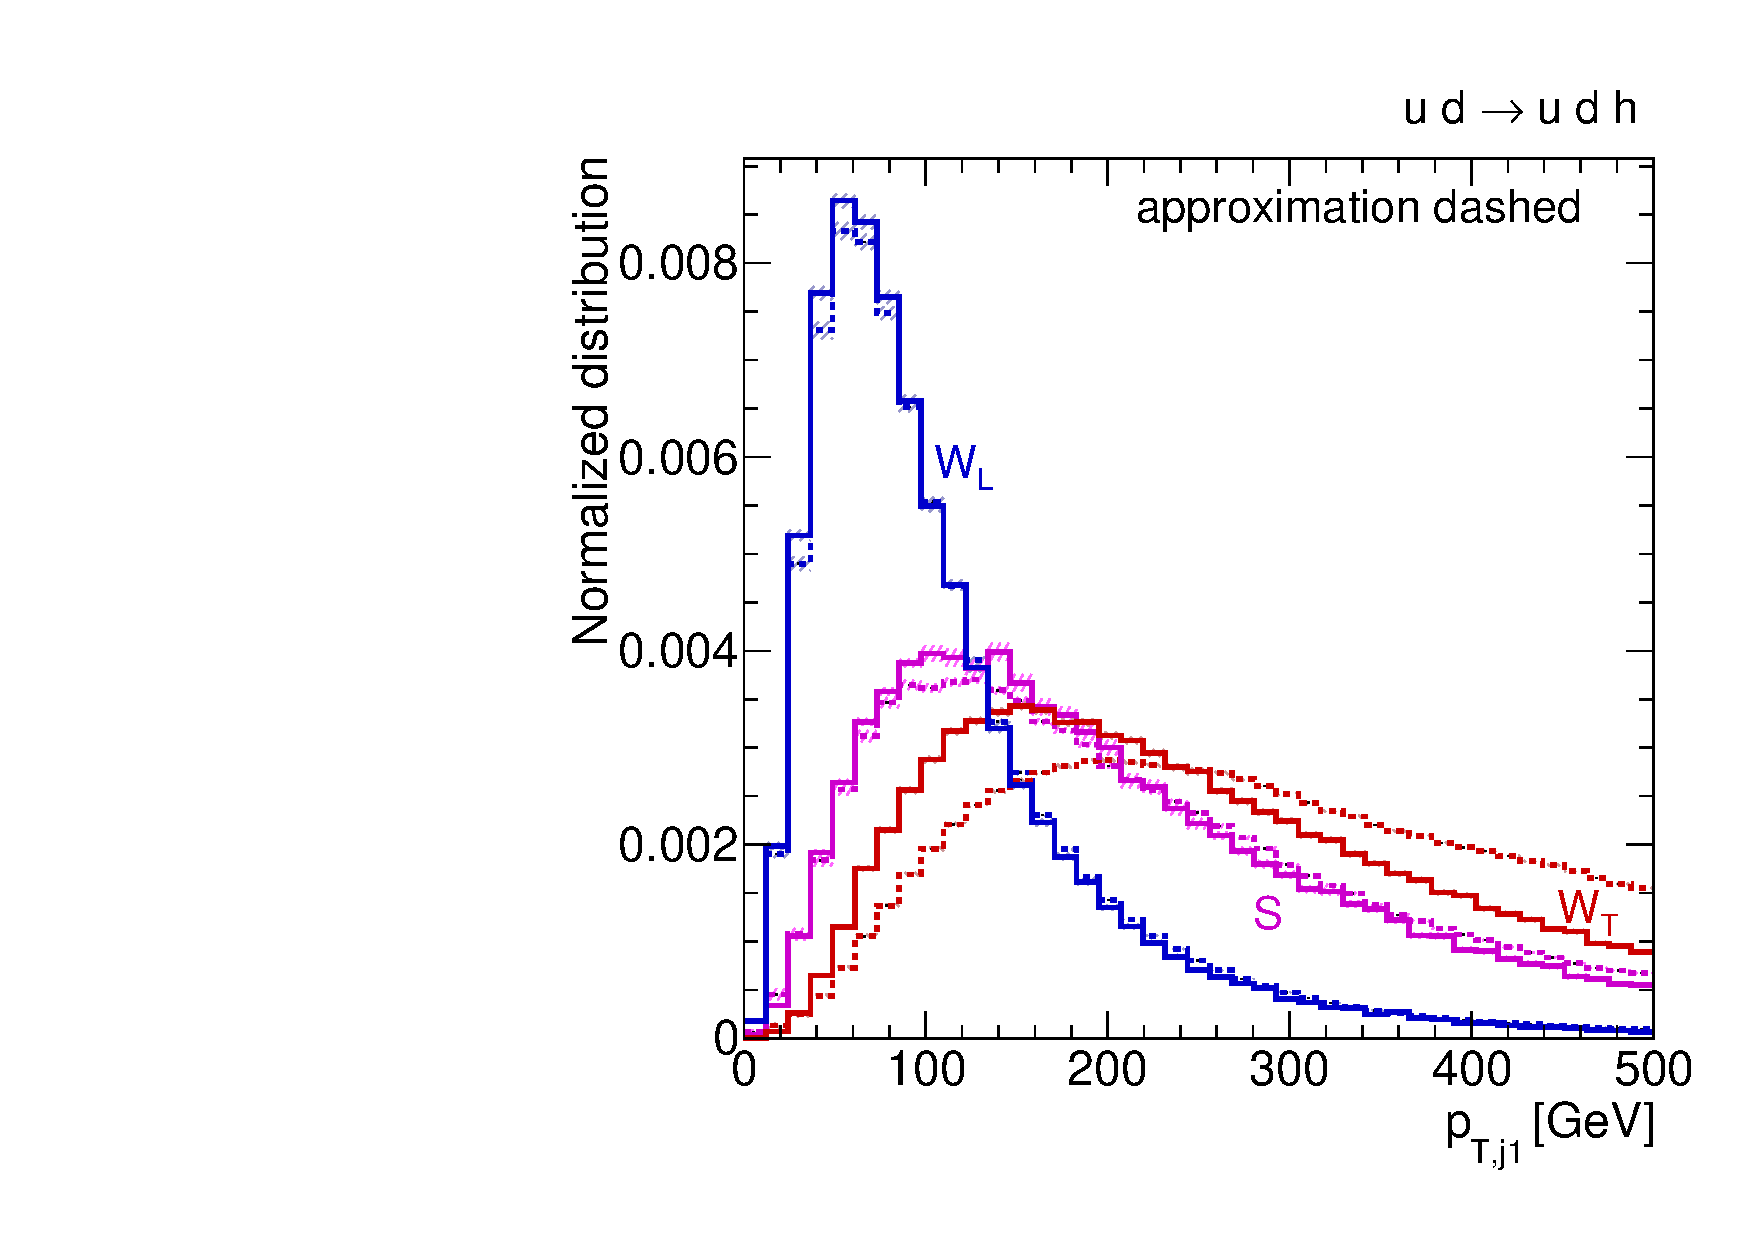
\includegraphics[width=0.43\textwidth]{fig/validity/WBF_ESA.pdf}
  \caption{Normalised WBF distributions of the tagging jets in the SM with
  a heavy Higgs, $m_h = 1$~TeV. Scalar mediators are compared to
  longitudinal and transverse $W$ bosons following
  Reference~\cite{polarized_ww}.
  The dotted lines give the corresponding predictions of the effective
  $W$ and scalar approximations, Equation\;\eqref{eq:validity_splittings}.}
  \label{fig:validity_effective_scalar}
\end{figure}
%------------------------------------------------------------



%%%%%%%%%%%%%%%%%%%%%%%%%%%%%%%%%%%%%%%%%%%%%%%%%%%%%%%%%%%%
\subsection{Which observables to study}
%%%%%%%%%%%%%%%%%%%%%%%%%%%%%%%%%%%%%%%%%%%%%%%%%%%%%%%%%%%%

%------------------------------------------------------------
\begin{figure}[t]
%  \centering
  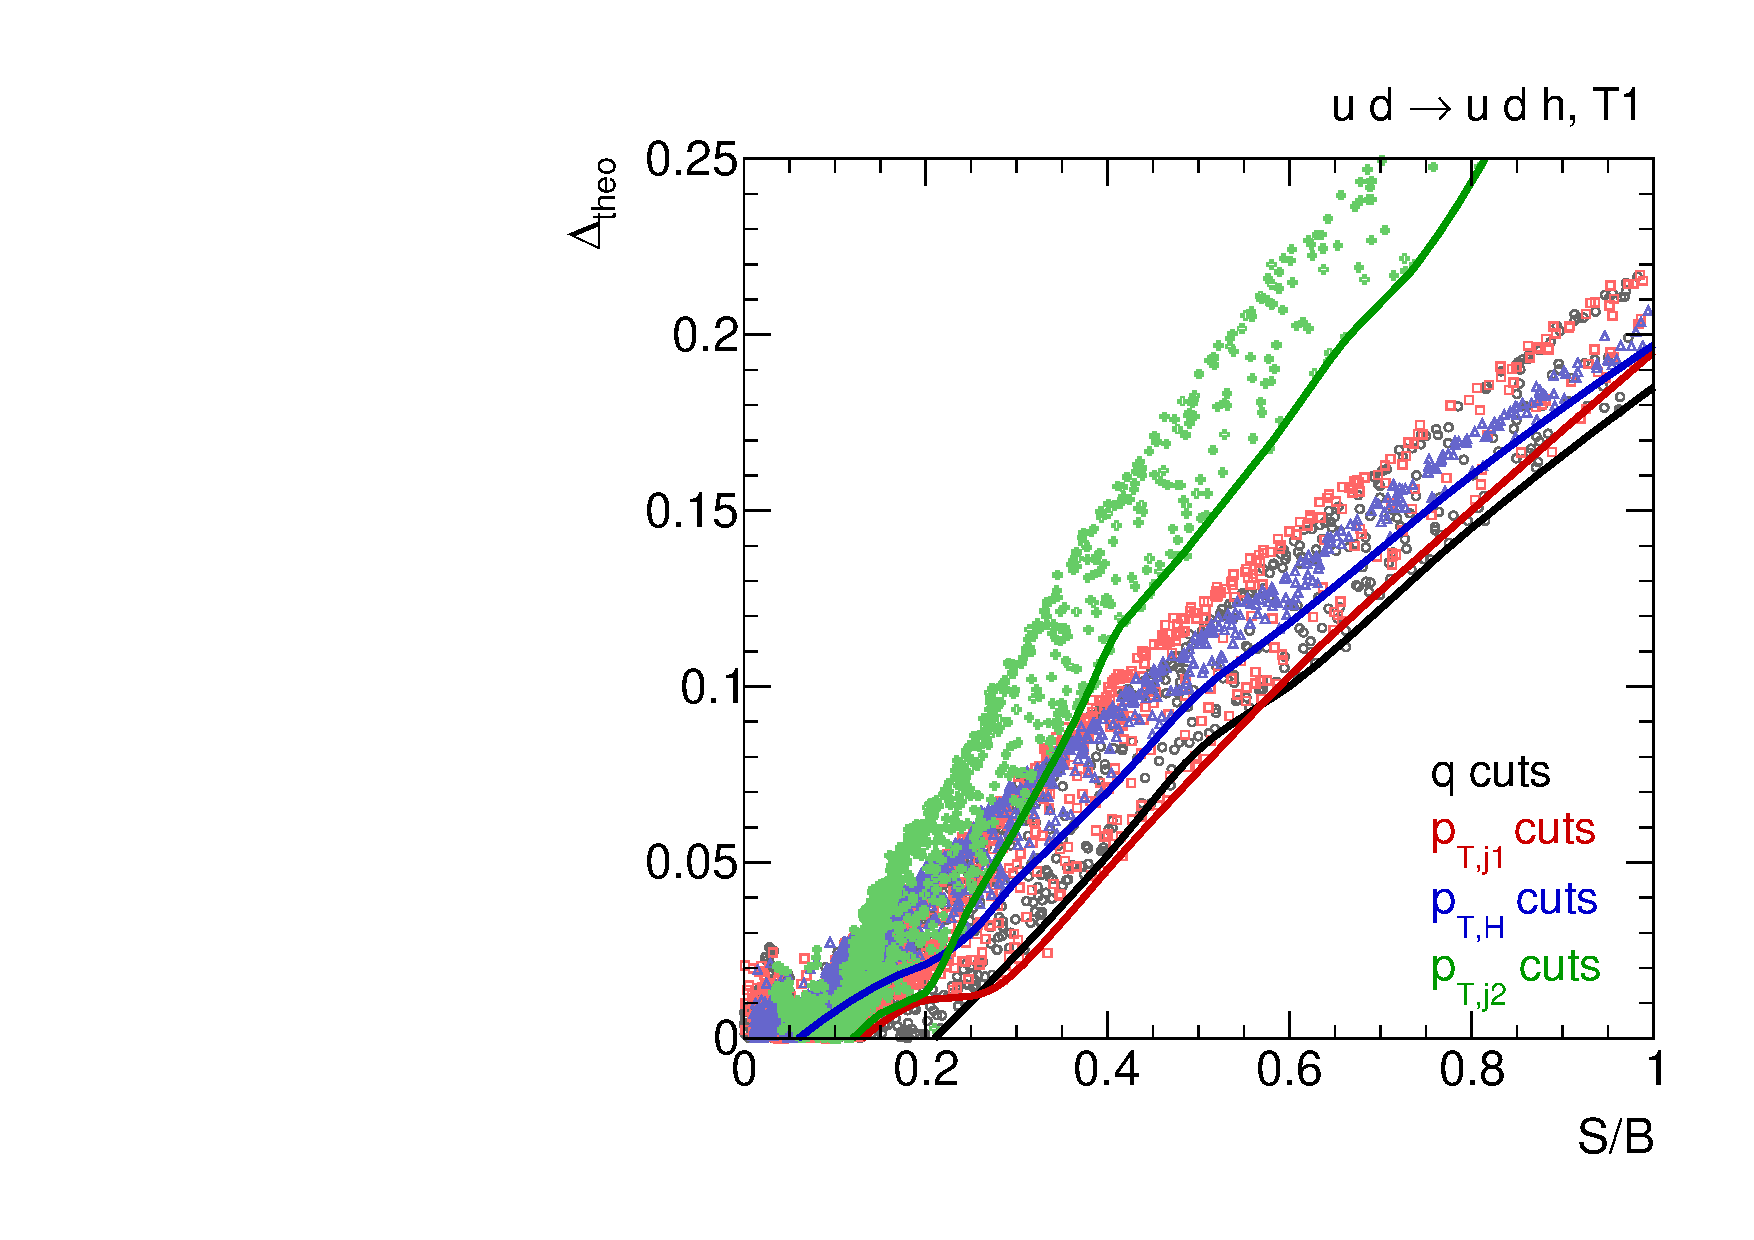
\includegraphics[width=0.43\textwidth]{fig/validity/WBF_cuts_T1_SB.pdf}
  \hspace*{0.05\textwidth}
  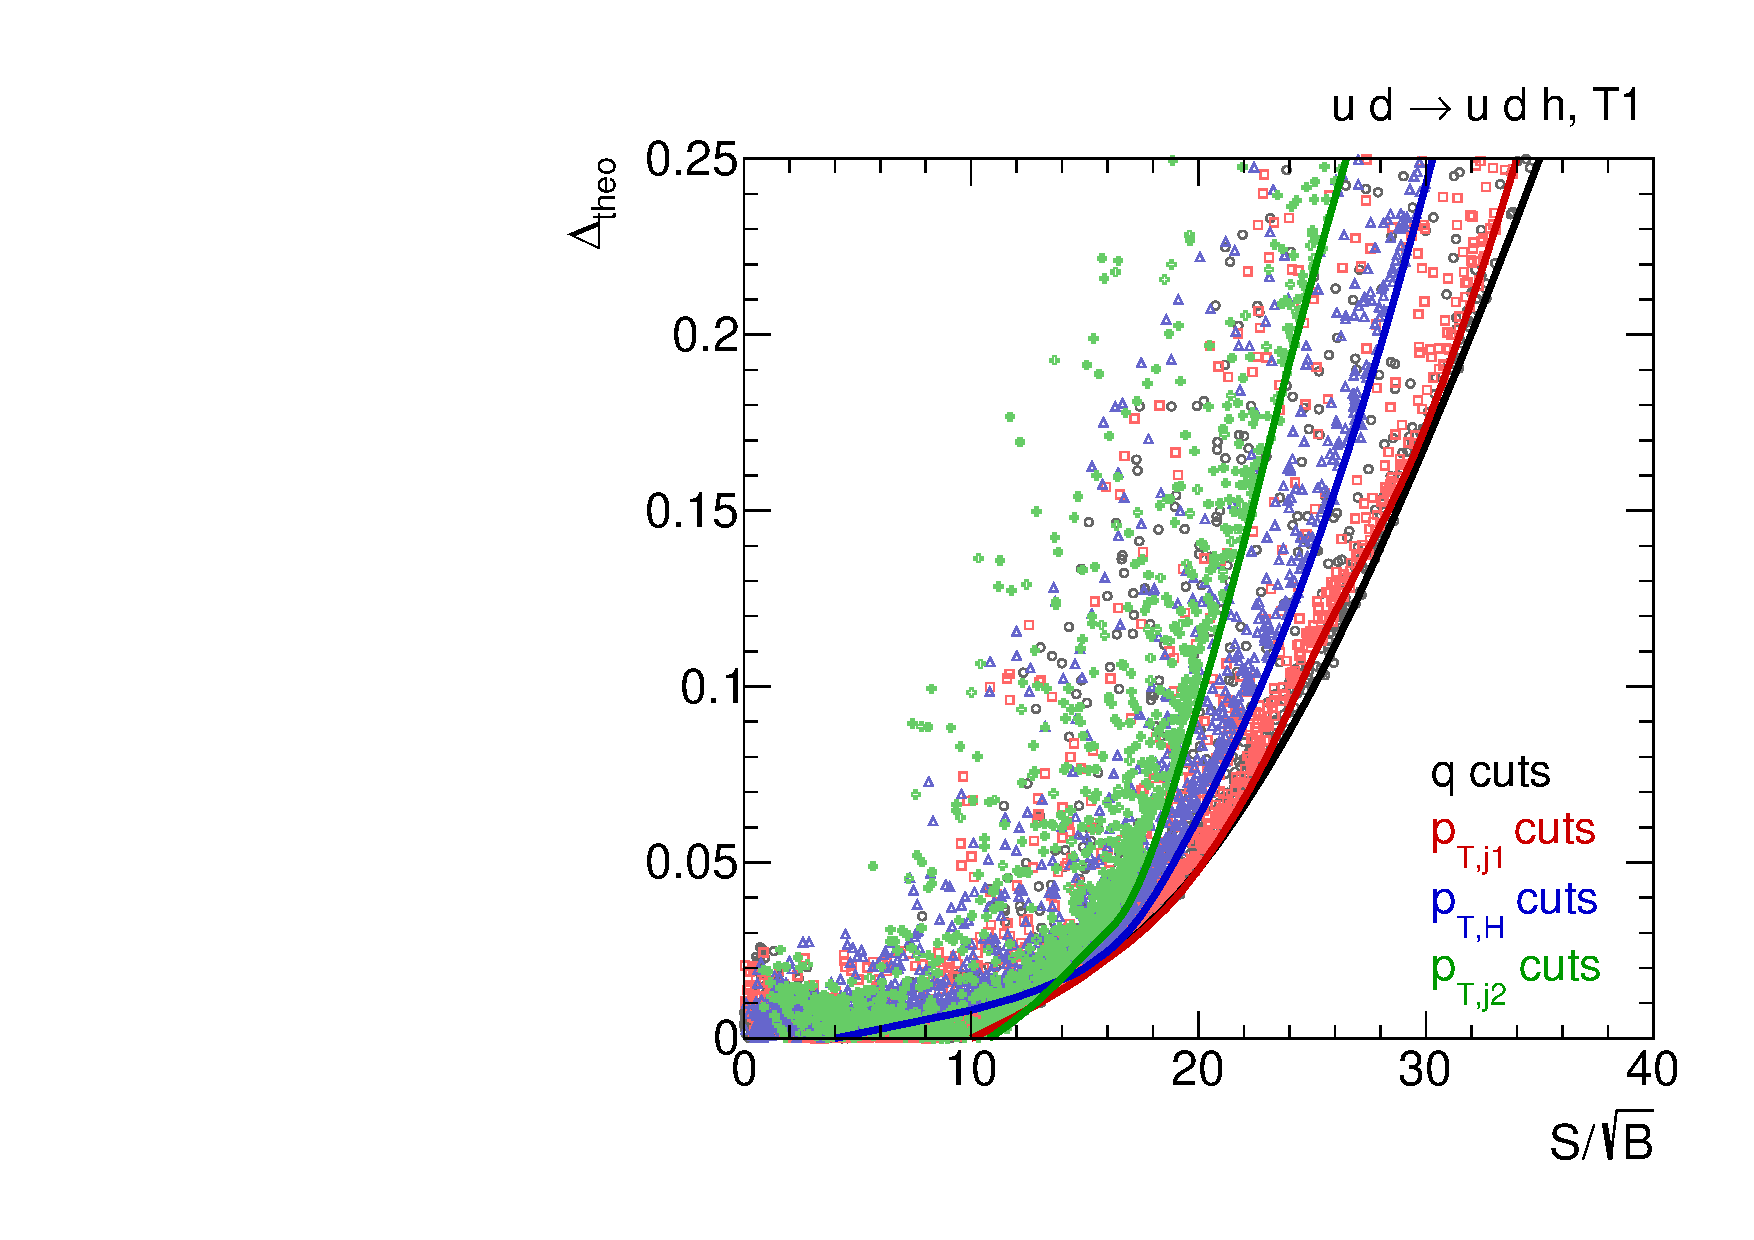
\includegraphics[width=0.43\textwidth]{fig/validity/WBF_cuts_T1_SsqrtB.pdf}
  \caption{Experimental reach in systematics-driven and
    statistics-driven channels vs theoretical uncertainties of the
    dimension-six description. Each point corresponds to a window
    $x_\text{min,max}$ in one of the four momentum observables that leaves a signal
    cross section of at least 20~fb.}
  \label{fig:validity_cuts}
\end{figure}
%------------------------------------------------------------

Now that it is clear that we cannot further improve the agreement
between the vector triplet and its dimension-six approximation by adding
a heavy scalar as a simplified model, we go back to the original
problem: how can we best use the dimension-six approximation for limit
setting, and do the shortcomings shown in
\autoref{fig:validity_squared_separate} harm this approach?

We know that in our LHC analysis we should avoid angular correlations
of the tagging jets, like $\Delta \eta_{jj}$ or $\Delta
\phi_{jj}$. Instead, we can use momentum-related kinematic variables
like
%
\begin{align}
 x \in \left\{  q, \, p_{T,j_1}, \, p_{T,j_2}, \, p_{T,h} \right\} \; .
\label{eq:validity_variables}
\end{align}
%
An acceptance cut $x > x_\text{min}$ on any of those variables
projects out the interesting phase-space regions, while the cut $x <
x_\text{max}$ ensures the validity of an effective theory
description. If $x_\text{min} > x_\text{max}$ the dimension-six
description is not useful. For each window $x_\text{min,max}$ we can
compute the contribution to the theoretical uncertainty
%
\begin{align}
  \Delta_\text{theo} (x_\text{min,max}) 
= \left| \frac {\sigma_\text{D6} - \sigma_\text{full}} {\sigma_\text{full}} \right| \; ,
\label{eq:validity_err_th}
\end{align} 
%
as well as the statistics-driven and systematics-driven significances
%
\begin{align}
  \frac{S}{B} (x_\text{min,max}) 
= \left| \frac {\sigma_\text{full} - \sigma_\text{SM}} {\sigma_\text{SM}} \right| 
\qquad \text{and} \qquad 
  \frac{S}{\sqrt{B}} (x_\text{min,max}) 
= \sqrt{L} \, \left| \frac {\sigma_\text{full} - \sigma_\text{SM}} {\sqrt{\sigma_\text{SM}}} \right| \; ,
\label{eq:validity_err_ex}
\end{align}
%
where $L = 30~\ifb$ is used as a toy number.

The question is for which
observable $x$ we find the largest $S/B$ and $S/\sqrt{B}$ values while
keeping $\Delta_\text{theo}$ small.  In \autoref{fig:validity_cuts} we show
the correlations between theoretical uncertainty and experimental
reach for the variables defined in Equation\;\eqref{eq:validity_variables} for a
parton-level analysis as defined in Equation\;\eqref{eq:validity_def_wbf}. We see
that the momentum transfer $q$ or the leading tagging jet's
$p_{T,j_1}$ lead to the envelopes with the highest significance for a
given theoretical uncertainty $\Delta_\text{theo}$. This indicates
that the leading tagging jet's transverse momentum is the best way of
experimentally accessing the momentum flow through the hard process,
at least for the hard parton-level process with only two tagging
jets.





%%%%%%%%%%%%%%%%%%%%%%%%%%%%%%%%%%%%%%%%%%%%%%%%%%%%%%%%%%%%
\section{Conclusions}
\label{sec:validity_conclusions}
%%%%%%%%%%%%%%%%%%%%%%%%%%%%%%%%%%%%%%%%%%%%%%%%%%%%%%%%%%%%

An effective field theory for the Higgs sector offers a theoretically
well-defined, efficient, and largely model-independent language to
analyse extensions of the Standard Model in both rate measurements and
kinematic distributions. A fit of dimension-six operators to LHC Higgs
measurements works fine~\cite{Corbett:2015ksa} and constitutes the
natural extension of the Higgs couplings analyses of Run~I.  Most of
the relevant higher-dimensional operators correspond to simple
coupling modifications, supplemented by four operators describing new
Lorentz structures in the Higgs coupling to weak
bosons~\cite{Corbett:2015ksa}.

In this paper we have studied the validity of this approach from the
theoretical side.  We know that at the LHC a clear hierarchy of
electroweak and new physics scales cannot be guaranteed, the question
is whether dimension-six operators nevertheless capture the
phenomenology of specific UV-complete theories with sufficient
accuracy.  We have systematically compared a singlet Higgs portal
model, a two-Higgs doublet model, scalar top partners, and a heavy
vector triplet to their dimension-six EFT descriptions, based on the
linear realisation of electroweak symmetry breaking with a Higgs
doublet.  We have analysed the main Higgs production and decay
signatures, covering rates as well as kinematic distributions.

We have found that the dimension-six operators provide an adequate
description in almost all realistic weakly coupled scenarios. Shifts
in the total rates are well described by effective operators.
Kinematic distributions typically do not probe weakly interacting new
physics with sufficient precision in the high-energy tails to
challenge the effective operator ansatz.  This is obvious for the
extended scalar models, where new Lorentz structures and
momentum-dependent couplings with dramatic effects in LHC
distributions only appear at the loop level.  A loop-suppressed
effective scale suppression $E^2/(4 \pi \Lambda)^2$ has to be compared
with on-shell couplings modifications proportional to $v^2/\Lambda^2$.
Only phase space regions probing energies around $4 \pi v \approx
3$~TeV significantly constrain loop contributions in the Higgs sector
and eventually lead to breakdown of the effective field theory. In
turn, a simple dimension-six descriptions will capture all effects that
are expected to be measurable with sufficient statistics at the LHC
Run II.  On the other hand, the vector triplet model shows that
modifications of the gauge sector can generate effects in LHC
kinematics at tree level. However, we again find that for weakly
interacting models and phenomenologically viable benchmark points they
are described well by an appropriate set of dimension-six
operators.

%-----------------------------------------------------------
\begin{table}[t] \renewcommand{\arraystretch}{1.2} \centering
\begin{tabular}{ll c ccc} \toprule Model & Process &\hspace*{1em}&
\multicolumn{3}{c}{EFT failure} \\ \cmidrule{4-6} & && resonance &
kinematics & matching \\ \midrule singlet & on-shell $h \to 4 \ell$,
WBF, $Vh$, \dots && & & \largex \\ & off-shell WBF, \dots && &
\brlargex & \largex \\ & $hh$ && \largex & \largex & \largex \\ 2HDM &
on-shell $h \to 4 \ell$, WBF, $Vh$, \dots && & & \largex \\ &
off-shell $h \to \gamma \gamma$, \dots && & \brlargex & \largex \\ &
$hh$ && \largex & \largex & \largex \\ top partner & WBF, $Vh$ && & &
\largex \\ vector triplet & WBF && & \brlargex & \largex \\ & $Vh$ &&
\largex & \brlargex & \largex \\ \bottomrule
\end{tabular}
 \caption{Possible sources of failure of dimension-six Lagrangian at the
LHC.  We use parentheses where deviations in kinematic distributions
appear, but are unlikely to be observed in realistic scenarios.}
 \label{tbl:validity_differences}
\end{table}
%-----------------------------------------------------------


Three sources for a possible breakdown of the dimension-six description
are illustrated in \autoref{tbl:validity_differences}\footnote{Forcing the EFT
approach into a spectacular breakdown was the original aim of this
paper, but to our surprise this did not happen.}: First, the EFT
cannot describe light new resonances. Such a signature at the LHC
would be an obvious signal to stop using the EFT and switch to
appropriate simplified models.  Second, selected kinematic
distributions fail to be described by the dimension-six Lagrangian, in
particular for Higgs pair production.  Deviations in the high-energy
tails of WBF and Higgs-strahlung distributions on the other hand are
too small to be relevant in realistic weakly coupled scenarios. These
two cases do not threaten LHC analyses in practice.

The third issue with the dimension-six EFT description is linked to
matching in the absence of a well-defined scale hierarchy.  Even with
only one heavy mass scale in the Lagrangian, the electroweak VEV
together with large couplings can generate several new physics scales,
defined by the masses of the new particles.  A linear EFT description,
which is justified by the SM-like properties of the newly discovered
Higgs boson, should in principle be matched in the phase where the
electroweak symmetry is unbroken. Such a procedure is blind to
additional scales induced by the electroweak VEV, potentially leading
to large errors in the dimension-six approximation.  Including
$v$-dependent terms in the Wilson coefficients, which corresponds to
matching in the broken phase, can significantly improve the EFT
performance. We have explicitly demonstrated this for all the models
considered in this paper.

None of these complications with the dimension-six description presents
a problem in using effective operators to fit LHC Higgs data.  They
are purely theoretical issues that need to be considered for the
interpretation of the results.


%%%%%%%%%%%%%%%%%%%%%%%%%%%%%%%%%%%%%%%%

While a dimension-six Higgs analysis at the LHC cannot be considered the
leading part of a consistent effective theory, it describes the
effects of weakly interacting extensions of the Higgs-gauge sector very
well~\cite{too_long}. In this brief study we have answered two practical
question concerning such a dimension-six analysis for Run~II.

First, a priori it is not clear if squared dimension-six terms should be
included in calculations. We have studied two particularly challenging
parameter points of a vector triplet model for $Vh$ production and for
weak-boson-fusion Higgs production. For both processes we find that
the dimension-six squared term avoids negative rate predictions in the
$m_{Vh}$ or $p_{T,V}$ distributions of $Vh$ production and in the
$p_{T,j_1}$ distribution of weak boson fusion. Even for cases with a
constructive interference between the dimension-six and the Standard
Model contributions, it turns out that including the dimension-six
squared term improves the agreement of kinematic distributions between
the full model and the dimension-six approximation. Ultimately, this
translates into a better agreement in the expected exclusion
limits\footnote{Similar conclusions in a different framework have recently
been published in Reference~\cite{gino}.}.

Second, we have attempted to improve the agreement between the full
model and our approximation by using a simplified model. The only
significantly simpler model than a mixing gauge extension is an
extended scalar sector. While the corresponding deviations between the
full model and the dimension-six approximation are phenomenologically
hardly relevant, we find that such an additional scalar improves the
modelling of kinematic distributions of the kind $m_{Vh}$ and
$p_{T,j_1}$ where the dimension-six description breaks down. However,
this comes at the cost of significant deviations in the dominant
interference terms. Moreover, once we include angular correlations
like $\Delta \eta_{jj}$ or $\Delta \phi_{jj}$ in weak boson fusion,
the simplified model fails badly. The difference can be traced to the
divergence structure of the corresponding splittings.

Seeing that the dimension-six approach is still the better simple model
to describe new physics in WBF distributions, we have finally analysed
which phase-space regions provide an interesting window to new physics
while being well described by the dimension-six approximation.  We have
demonstrated that the leading tagging jet's $p_T$ distribution is
particularly suited for such a search for new physics.

% 

\setchapterpreamble[ur]{%
\dictum[D.~Adams~\cite{adams2002salmon}]{%
Anything that is in the world when you’re born is normal and ordinary and is just a natural part of the way the world works.

Anything that's invented between when you’re fifteen and thirty-five is new and exciting and revolutionary and you can probably get a career in it.

Anything invented after you're thirty-five is against the natural order of things.%
}%
\vspace*{2cm}}



%%%%%%%%%%%%%%%%%%%%%%%%%%%%%%%%%%%%%%%%%%%%%%%%%%%%%%%%%%%%
\chapter{Better Higgs measurements through information geometry}
\label{chapter:information}
%%%%%%%%%%%%%%%%%%%%%%%%%%%%%%%%%%%%%%%%%%%%%%%%%%%%%%%%%%%%

\firstword{W}{ith the results of the last chapter,} we rest assured
that many potential signatures of new physics in Higgs observables can
be parametrised by dimension-six operators. The next question is how
the corresponding Wilson coefficients can be measured as precisely as
possible. In this chapter we develop statistical tools based on
information geometry that can help to optimise such measurements.

After an introduction in \autoref{sec:information_intro}, in
\autoref{sec:information_formalism} we summarize the statistics of the
measurement process, define the Fisher information, and discuss what
constitutes an optimal measurement. In
\autoref{sec:information_madfisher} we apply these general ideas to
LHC physics and develop an algorithm to calculate the Fisher
information in particle physics processes. We also discuss some
aspects of information geometry particular to effective field
theories. In \autoref{sec:information_application_even} we use our
formalism to understand how $CP$-even dimension-six operators can be
measured in a range of Higgs channels.
Section~\autoref{sec:information_application_odd} focusses on the
measurement of $CP$ violation. We demonstrate how our approach can be
extended to describe systematic uncertainties, and link it to other
statistical tools, in \autoref{sec:information_extensions}, and
finally give our conclusions in \autoref{sec:information_conclusions}.

Most of the research presented in this chapter was previously
published in Reference~\cite{Brehmer:2016nyr}. The results and their
presentation, including nearly all plots and tables as well as part of
the text, are identical to that in this article. The exception is
\autoref{sec:information_application_odd}, which is based on ongoing
and yet unpublished work~\cite{Brehmer:CPV_information}.



%%%%%%%%%%%%%%%%%%%%%%%%%%%%%%%%%%%%%%%%%%%%%%%%%%%%%%%%%%%%
\section{Introduction}
\label{sec:information_intro}
%%%%%%%%%%%%%%%%%%%%%%%%%%%%%%%%%%%%%%%%%%%%%%%%%%%%%%%%%%%%

Having established that the dimension-six operators of the linear
Higgs effective theory capture the indirect signatures of many
scenarios of new physics, we now analyse how its parameters, the
Wilson coefficients $f_i/\Lambda^2$, can be measured most efficiently
at the LHC. This is a highly non-trivial problem for two reasons:
first, the Higgs properties form a high-dimensional parameter
  space. In \autoref{sec:foundations_heft_operators} we showed that
even after removing redundant operators and generously neglecting
those with tight limits from electroweak precision measurements or
flavour constraints, we are left with thirteen dimension-six operators
relevant for Higgs physics. The Higgs-gauge interactions, for
instance, are affected by seven of these operators, equivalent to a
range of different kinematic structures or forms of momentum
dependence. The second challenge comes from the complicated
  kinematics of some of the Higgs production channels and decay
modes. For example, Higgs production in weak boson fusion with a decay
$h \to W^+W^- \to (\ell^+ \nu) (\ell^- \overbar{\nu})$ is a $2 \to 6$
process even at parton level, and only made more complicated by
additional QCD radiation. Such a high-dimensional phase space defines
a large number of kinematic observables, and it is often not obvious
which of them carry information on the theory parameters of
interest. The relation between the high-dimensional parameter space
and the potentially high-dimensional phase space is (at parton level)
encoded in the amplitudes or Feynman diagrams, of which there can
easily be hundreds for a given process.

\emph{Traditional analysis methods} typically begin with simple
selection cuts on standard kinematic observables such as energies,
momenta, angles, or invariant masses. This is often followed by the
estimation of background contributions with a mixture of simulational
and data-driven methods. The final statistical analysis typically
relies on total event counts or on histograms of kinematic
observables.  These techniques are very intuitive and all steps are
transparent. They they work well for simple signatures, such as a
resonance peak on top of a smooth background, as in the discovery of
the $gg \to h \to \gamma \gamma$
signal~\cite{Aad:2012tfa,Chatrchyan:2012xdj}. This approach requires a
careful tailoring of the strategy to each question, and does not scale
well with the complexity of the theory questions or the kinematics of
the processes.

At the other end of the spectrum, the LHC collaborations increasingly
rely on measurement strategies based on high-level statistical
tools~\cite{cranmer:nips2016}. Some of them are based on the structure
of the \emph{matrix elements} contributing to the process. In the
matrix element method~\cite{Kondo:1988yd, Abazov:2004cs, Gao:2010qx,
  Alwall:2010cq, Avery:2012um, Andersen:2012kn, Campbell:2013hz,
  Artoisenet:2013vfa, Martini:2015fsa, Gritsan:2016hjl}, the
differential cross section expected from a given model hypothesis at a
specific phase-space point, or the ratio of two such expected rates,
is directly used as an observable. The detector response is estimated
by convuluting this expression with suitable transfer
functions. Shower deconstruction~\cite{Soper:2011cr, Soper:2012pb} and
even deconstruction~\cite{Soper:2014rya} extend this concept to the
parton shower to take into account the information encoded in jet
substructure. Optimal observables~\cite{Atwood:1991ka, Davier:1992nw,
  Diehl:1993br} apply the same idea to the measurement of a small
theory parameter. All these tools intrinsically make full use of the
information encoded in the underlying field theories, but rely on an
approximate description of the detector systems. They are particularly
useful in channels with not too many particles in the final state that
can be reconstructed precisely. Large final-state multiplicities
require a high-dimensional integration and is computationally
expensive. Finally, matrix-element-based tools generally rely on the
comparison of two discrete hypotheses or for the measurement of one
model parameter, \ie one direction in theory space. Applying these
methods to high-dimensional theory spaces such as Higgs effective
field theory often requires a discretization of the theory space,
which can be computationally expensive, and care has to be taken to
avoid dependencies on EFT basis choices.

A second class of statistical tools falls under the category of
\emph{likelihood-free inference}~\cite{cranmer:nips2016}. They are
mostly based on (supervised) machine learning techniques:
sophisticated interpolation techniques, such as boosted decision trees
and neural networks, are used to describe patterns in a set of
training samples. This approach is agnostic about the amplitudes
describing a process. The methods with which the input samples are
generated is irrelevant. Unlike simple likelihood-based methods, these
samples can be based on data as well as complicated Monte-Carlo
simulations with a parton shower and full detector simulation. New
technologies are developed at an impressive
pace~\cite{Cranmer:2015bka, Louppe:2016ylz, Louppe:2016aov,
  Cranmer:2016lzt, Baldi:2016fzo}. These tools are applied to problems
at all steps of the analysis process, ranging from
tracking~\cite{Brehmer:ghost_probability} over the analysis of jet
substructure~\cite{Cogan:2014oua, Baldi:2014pta, deOliveira:2015xxd,
  Almeida:2015jua, Baldi:2016fql, Guest:2016iqz, Komiske:2016rsd,
  Kasieczka:2017nvn, Louppe:2017ipp} to the discrimination between
signal and background hypotheses~\cite{Baldi:2014kfa, Searcy:2015apa,
  Santos:2016kno, Alves:2016htj} and finally to the statistical
testing of model hypotheses~\cite{Buckley:2011kc, Bornhauser:2013aya,
  Bechtle:2017vyu}. For complicated problems, multivariate tools often
outperform traditional approaches. However, their inner structure is
often convoluted and not necessarily very unintuitive; and it is not
always clear which physical structures these ``black boxes'' are
sensitive to.

\newparagraph
%
With these wide range capabilities, it is increasingly important that
we can understand and characterise the information contained in
particle physics processes. The design of event selections and
analysis strategies requires clearly defined guidelines. We present an
approach to these problems based on information
geometry~\cite{efron1975, amari1982}. It offers tools that are
intrinsically designed for continous parameter spaces of arbitrary
dimensionality, independent of basis choices and without the need for
any discretization of the model hypothesis.

The central object in our approach is the \emph{Fisher information}
matrix. According to the Cram\'er-Rao bound~\cite{Rao:1945,
  Cramer:1946}, it quantifies the maximum knowledge on
theory parameters that we can derive in a measurement, independent of
the analysis strategy. This allows us to calculate the best possible
precision with which theory parameters can be measured with any
multivariate black-box analysis. Also, the Fisher information defines
a metric in the space of theory parameters. This provides an intuitive
geometric interpretation for the discrimination power of an
experiment. From a practical perspective, it gives us a handle on the
linearisation of observables in terms of new physics parameters, as we
demonstrate in the next section.

Two objects are particularly interesting for LHC physics.  First, the
distribution of the differential information over phase space defines
the relevance of different phase-space regions for an analysis and
should motivate the design of event selections. Second, we can
calculate the information contained in individual kinematic
observables and compare it to the full Fisher information. This
determines the most important observables and allows us to compare the
power of traditional histogram-based analyses to that of modern
multivariate tools.

We develop an algorithm, which we call \toolfont{MadFisher}, that can
calculate the Fisher information for arbitrary perturbative
particle-physics processes based on Monte-Carlo methods. We can
calculate the quantities outlined above, each designed to answer
different practical questions:
%
\begin{itemize}
\item \emph{full Fisher information}: what is the maximum precision
  with which continous model parameters can be measured in a process?
    %
\item \emph{differential Fisher information}: how is the information
  on model parameters distributed over phase space?
    %
\item \emph{information in distributions}: how well can we measure
  model parameters based on individual kinematic observables, rather
  than the information in the full high-dimensional phase space?
    %
\item \emph{global geometry}: which role do non-linear terms in the
  theory parameters play?
\end{itemize}

\newparagraph
%
As a first application we calculate the information on $CP$-even
dimension-six operators in WBF Higgs production with a decay into tau
pairs, focussing on the kinematic structures defined by the tagging
jets and their sensitivity to the Higgs-gauge coupling structure. We
then analyse WBF Higgs production in the four-lepton mode to see how
much additional information is contained in the decay kinematics. The
final channel we analyse is Higgs production in association with a
single top.

The next question we tackle with the information geometry approach is
how $CP$ violation can be measured in Higgs observables. We aim to
disentangle genuine $CP$-violating signatures from those kinematic
features of $CP$-odd operators that can also arise from $CP$-even
physics. Finally, we demonstrate how systematic uncertainties can be
treated in our approach, and compare the Fisher information to other
statistical tools.

\newparagraph
%
The Fisher information has been commonly used in the field of
gravitational wave detection~\cite{Jaranowski:1994xd}, but has
received much less attention in particle physics~\cite{CMS:2016kgk,
  Ferreira:2017ymn}. To the best of our knowledge, most of the tools
presented in Reference~\cite{Brehmer:2016nyr} and in this chapter are
innovative at least for this field.


% After its experimental discovery~\cite{higgs,discovery} the Higgs
% boson and its properties have immediately become one of the most
% important and active fields of searches for physics beyond the
% Standard Model at the LHC.  In the Lagrangian language of fundamental
% physics, the Higgs properties can be described by a continuous and
% high-dimensional parameter space, for instance in terms of Wilson
% coefficients in an effective field theory
% (EFT)~\cite{eftfoundations,eftorig,eftreviews}. One of the main
% features of moving from simple coupling modifications to
% higher-dimensional operators is that we can now include kinematic
% distributions in these searches~\cite{higgs_fit,yr4}. A common
% challenge of all Higgs analyses is how to navigate the vast family of
% phase-space distributions.

% Responding to the overwhelming amount of search strategies, we expect
% the LHC collaborations to focus more and more on high-level
% statistical tools, including hypothesis tests based on multivariate
% analysis with machine learning or the matrix element
% method~\cite{statistics,kyle_review}. Historically, these tools
% compare two discrete hypotheses, and applying them to continuous,
% high-dimensional parameter spaces is computationally expensive.  Only
% recently, machine learning techniques have been extended to include
% inference on such continuous high-dimensional parameter
% spaces~\cite{machine_learning}.  With these capabilities, it becomes
% increasingly important to be able to effectively characterize the
% information contained in these distributions.  We present an approach
% based on information geometry~\cite{information-geometry},
% intrinsically designed to study continuous parameter spaces of
% arbitrary dimensionality without the need for any discretization of
% the hypothesis. We use this to compare and improve Higgs measurement
% strategies.

% Our central object is the Fisher information matrix. Through the
% Cram\'er-Rao bound it determines the maximum knowledge on model
% parameters that we can derive from an
% observation~\cite{cramer-rao,information-applications}. In that sense the
% Cram\'er-Rao bound for the Fisher information plays a similar role as
% the Neyman-Pearson lemma~\cite{neyman-pearson} plays for a discrete
% hypothesis test and the log-likelihood ratio: it allows us to define
% and to compute the best possible outcome of any multivariate black-box
% analysis~\cite{kyle_review,madmax1}. In addition, the Fisher
% information matrix defines a metric in the space of model parameters,
% which not only provides an intuitive geometric picture, but also gives
% us a handle on the linearization of the observable in terms of new
% physics effects.

% When we apply our information geometry framework to Higgs physics, in
% particular to analyses of the dimension-6 Higgs Lagrangian, we can
% tackle questions of the kind:
% %
% \begin{itemize}[label=\raisebox{0.1ex}{\scriptsize$\bullet$}]
% \item What is the maximum precision with which we can measure
%   continuous model parameters?
% \item How is the information distributed over phase space?
% \item How much of the full information is contained in a given set of
%   distributions?
% \item Which role do higher-dimensional corrections in the EFT
%   expansion play?
% \end{itemize}
% %

% We demonstrate our approach using three examples: Higgs production in
% weak boson fusion (WBF)~\cite{dave_thesis} with its tagging-jet
% kinematics~\cite{tagging} is well known to probe many aspects of the
% Higgs-gauge coupling structure~\cite{phi_jj}. Focusing on the WBF
% production kinematics we first analyze its combination with a Higgs
% decay to tau leptons~\cite{wbf_tau}. This will for example allow us to
% estimate how much of the entire information on higher-dimensional
% operators is typically included in the leading tagging jet
% distributions. Combining WBF production with a Higgs decay to $ZZ^*$
% pairs we can test how much additional information is included in the
% decay distributions. Conceptually, this contrasts two ways to
% constrain the same effective Lagrangian via large momentum flow
% through the relevant vertices or via precision observables~\cite{higgs_fit}.
% Finally, we will test how useful Higgs production in association with
% a single top~\cite{top_higgs} is for a dimension-6 operator analysis.

% In a set of appendices we give a worked-out simple example for our
% approach, explain how we compute the Fisher information, show more
% information on our example processes, indicate how systematic or
% theory uncertainties can be included, and discuss the relation of our
% approach to standard log-likelihood ratios.



%%%%%%%%%%%%%%%%%%%%%%%%%%%%%%%%%%%%%%%%%%%%%%%%%%%%%%%%%%%%
\section{Information geometry}
\label{sec:information_formalism}
%%%%%%%%%%%%%%%%%%%%%%%%%%%%%%%%%%%%%%%%%%%%%%%%%%%%%%%%%%%%

%%%%%%%%%%%%%%%%%%%%%%%%%%%%%%%%%%%%%%%%%%%%%%%%%%%%%%%%%%%%
\subsection{Fisher information and Cram\'er-Rao bound}
\label{sec:information_formalism_information}
%%%%%%%%%%%%%%%%%%%%%%%%%%%%%%%%%%%%%%%%%%%%%%%%%%%%%%%%%%%%

Any measurement uses experimental data $\boldx$ to calculate an
estimator $\hat{\boldtheta}(\boldx)$ of the unknown true value of some
parameters $\boldtheta$. The outcome of the experiment is described by
the probability distribution $f(\boldx | \boldtheta_0)$ that depends
on the true value $\boldtheta_0$, and thus the outcome of the
estimator also follows a probability distribution
%
\begin{equation}
  f( \hat{\boldtheta} | \boldtheta_0) = \intfatx f( \boldx | \boldtheta_0)  \; \delta \left(\hat{\boldtheta} - \hat{\boldtheta}(\boldx) \right)\,.
\end{equation}
%
Two key properties of this distribution characterize the
measurement. First, the bias of an estimator is given by the
difference of the expectation value
%
\begin{equation}
  \overbar{\boldtheta} \equiv E \left[ \hat{\boldtheta} \middle | \boldtheta_0 \right]
  \equiv \intfatthetahat \hat{\boldtheta} \, f( \hat{\boldtheta} | \boldtheta_0)  
\end{equation}
%
and the true value $\boldtheta_0$. An estimator is unbiased if the
expectation value is always equal to the true value,
%
\begin{equation}
  \overbar{\boldtheta} = \boldtheta_0 \,.
\end{equation}
%
Second, the variance
%
\begin{equation}
  \var  \left [ \hat{\theta} \middle | \theta_0 \right]
  \equiv E \left[ (\theta - \overbar{\theta} )^2\middle | \theta_0 \right] \,,
\end{equation}
%
or for more than one parameter its covariance matrix
%
\begin{equation}
  \cov  \left [ \hat{\boldtheta} \middle | \boldtheta_0 \right]_{ij}
  \equiv E \left[ (\theta_i - \overbar{\theta}_i )  (\theta_j - \overbar{\theta}_j ) \middle | \boldtheta_0 \right] \,,
\end{equation}
%
provides a measure of the precision. 
% In practice there is often a
% trade-off between minimizing the bias of an experiment and the
% variance.~\comment{Example, or citation, from Kyle's TASI slides?}

But how good can an estimator be? Clearly, any given experiment does
not allow the measurement of parameters with arbitrary precision. We
can make this statement more quantitatively. If the parameters
$\theta_i$ are continous, $f(\boldx | \boldtheta)$ is twice
differentiable in them, and if we can exchange this differentiation
with the integration over $\boldx$, we can calculate the \emph{Fisher
  information}
%
\begin{equation}
  I_{ij} (\boldtheta)
     = E \left[
      \frac {\partial \log f(\boldx |\boldtheta) }  {\partial \theta_i } \,
      \frac {\partial \log f(\boldx |\boldtheta) }  {\partial \theta_j }
      \middle| \boldtheta \right]
      = - E \left[
      \frac {\partial^2 \log f(\boldx |\boldtheta) } {\partial \theta_i \, \partial \theta_j}
      \middle| \boldtheta \right] \,.
    \label{eq:information_fisher_information}
\end{equation}
%
The \emph{Cram\'er-Rao bound}~\cite{Rao:1945, Cramer:1946} then states that the
covariance matrix of any estimator $\hat{\boldtheta}$ is bounded from
below by the inverse Fisher information:
%
\begin{equation}
  \cov \left[ \hat{\boldtheta} \middle| \boldtheta_0 \right]_{ab}
  \geq \pder {\overbar{\theta}_a} {\theta_i} (\boldtheta_0) \;
  I^{\,-1}_{\ \ ij} (\boldtheta_0)  \;
  \pder {\overbar{\theta}_b} {\theta_j} (\boldtheta_0) \,,
  \label{eq:information_cramer_rao_general}
\end{equation}
%
where we implicitly sum over repeated indices $i$, $j$.  In
particular, for an unbiased estimator
$\overbar {\boldtheta} = \boldtheta_0$ and
%
\begin{equation}
  \cov \left[ \hat{\boldtheta} \middle| \boldtheta_0 \right]_{ij}
      \geq I^{\,-1}_{\ \ ij} (\boldtheta_0)  \,. 
  \label{eq:information_cramer_rao_unbiased}
\end{equation}
%
In the one-dimensional case, this corresponds to a typical measurement
error of
%
\begin{equation}
  \Delta \theta \equiv \sqrt{\var [ \hat{\theta} | \theta_0 ] } \geq 1 / \sqrt{ I (\theta_0) }\,.
  \label{eq:information_cramer_rao_precision}
\end{equation}
%
In this way, the Fisher information matrix $I_{ij}$ encodes the
maximal precision with which parameters can be measured at an
experiment. Large entries in this matrix correspond to directions that
can be measured particularly precisely. On the other hand, an
eigenvector of the information matrix with corresponding eigenvalue
zero is a blind direction that can never be probed by the experiment.

The Fisher information has several useful properties. Unlike many
other statistical tools, it summarizes the sensitivity to \emph{all}
directions in theory space in one matrix, making it particularly
useful for high-dimensional parameter spaces. It is additive between
different measurements or between different phase-space regions in the
same experiment.
% This allows us to calculate the
% distribution of information over phase space.
Furthermore, a description of experiments in terms of the Fisher
information is independent of arbitrary basis choices: it is invariant
under the parameterization of the observables $\boldx$, and transforms
covariantly under a reparameterization of the theory parameters
$\theta \to \Theta (\theta)$,
%
\begin{equation}
  I_{ab} (\boldsymbol{\Theta}) = \pder {\theta_i} {\Theta_a} \, I_{ij} (\boldsymbol{\theta}) \, \pder {\theta_j} {\Theta_b} \,.
  \label{eq:information_information_covariant_transformation}
\end{equation}

As a symmetric and positive definite rank-two tensor, the Fisher
information defines a Riemannian metric\footnote{This is only strictly
  true in the absence of blind directions, otherwise the information
  matrix is only positive semi-definite and defines a pseudo-metric.}
on the theory space. This is the cornerstone of \emph{information
  geometry}~\cite{efron1975, amari1982}, which uses methods from
differential geometry to analyse the structure of the probability
distributions, or the relation between experiment and
models. Interpreted as a metric, the Fisher information defines a
distance measure between parameter points. First, we can define local
distance in the tangent space at some point $\boldtheta_a$,
%
\begin{equation}
  d_{\text{local}}( \boldtheta_b; \boldtheta_a ) = \sqrt{I_{ij} (\boldtheta_a) (\theta_{b\,i} - \theta_{a\,i}) (\theta_{b\,j}  - \theta_{a\,j} )} \,.
  \label{eq:information_local_distances}
\end{equation}
%
Contours of local distances translate the Fisher information in one
point into the minimal error ellipsoids according to the Cram\'er-Rao
bound. The distance values have an intuitive interpretation: if the
estimator is distributed according to a Gaussian around the true
value, $d_{\text{local}}( \boldtheta_b; \boldtheta_a )$ corresponds to
how unlikely it is to measure $\hat{\boldtheta} = \boldtheta_b$ if the
true value is $\boldtheta_0 = \boldtheta_a$, expressed in standard
deviations or ``sigmas''. In other words, in this limit the distance
measure is equivalent to the maximal expected significance with which
$\boldtheta_a$ can be excluded if $\boldtheta_b$ is true.

Goying beyond the tangent space, global distances can be defined along
geodesics,
%
\begin{equation}
  d(\boldtheta_a,\boldtheta_b)
  = \min_{\boldtheta(s)} \;
  \int_{s_a}^{s_b} \!\! \mathrm{d} s \; \sqrt{I_{ij} \tder {\theta_i (s)} s \tder {\theta_j (s)} s } \,,
  \label{eq:information_global_distances}
\end{equation}
%
providing a more general and symmetric notion of discrimination power
between two points without having to pick the true value of the
parameter.

% As an aside, the Fisher information also plays an important role in
% Bayesian inference. In Jeffrey's prior it is used to define an
% ``objective'' prior that is invariant under reparameterization, and
% according to the Bernstein-von~Mises theorem it describes the
% posterior mode in the asymptotic limit.




%%%%%%%%%%%%%%%%%%%%%%%%%%%%%%%%%%%%%%%%%%%%%%%%%%%%%%%%%%%%
\subsection{A simple example}
\label{sec:information_formalism_example}
%%%%%%%%%%%%%%%%%%%%%%%%%%%%%%%%%%%%%%%%%%%%%%%%%%%%%%%%%%%%

As a simple example, we calculate the Fisher information in a number
of event counts $n_c$ in different channels $c$. We assume that the
channels are independent and follow Poisson distributions with mean
values $\bar{n_c} = \nu_c$:
%
\begin{align}%
  f (\mathbf{n} |\boldnu) 
  = \prod_c \Pois (n_c | \nu_c) 
  = \prod_c \, \frac{\nu_c^{n_c} e^{-\nu_c}}{n_c!} \, .
\end{align}
%
Following \autoref{eq:information_fisher_information}, we can calculate the Fisher
information in terms of the Poisson means $\boldnu$. With
%
\begin{equation}
  \pder { \log f} {\nu_c} 
  = \pder {} {\nu_c}  \left[- \nu_c + n_c \log \nu_c - \log (n_c!) \right]
  = \frac {n_c} {\nu_c} - 1
\end{equation}
%
and
%
\begin{equation}
  \frac { \partial^2 \log f} {\partial \nu_c \partial \nu_{c'}} = - \frac {\delta_{c c'} \, n_c} {\nu_c^2} 
\end{equation}
%
we find
%
\begin{equation}
  I_{c c'} (\boldnu) \equiv - E \left[ \frac { \partial^2 \log f} {\partial \nu_c \partial \nu_{c'}} \middle| \boldnu \right] = \frac {\delta_{c c'} } {\nu_c} \,.
\end{equation}

\autoref{eq:information_information_covariant_transformation} allows us calculate
the Fisher information in terms of some theory parameters $\theta_i$
rather than the Poisson means $\nu_c$:
%
\begin{align}
  I_{ij}  (\boldtheta) = \sum_c \pder {\nu_c} {\theta_i} \, \frac 1 {\nu_c} \, \pder {\nu_{c}} {\theta_j} \,.
  \label{eq:information_simple_example_information}
\end{align}
%
At the LHC, the matrix $\partial \nu_c / \partial \theta_i$ is
determined by the luminosity, the relevant cross sections and
branching ratios, as well as acceptance and efficiency factors. For
instance, in the $\kappa$ framework for Higgs physics discussed in
\autoref{sec:foundations_heft_alternatives} it is trivial to calculate
the matrix $\partial \nu_c / \partial g_i$ in closed form. For each
channel this matrix is singular, which means it measures one direction
in parameter space and is blind to all orthogonal directions. At least
as many channels as parameters are required to make the combined
information in \autoref{eq:information_simple_example_information}
non-singular and remove all blind directions (assuming the channels do
not provide degenerate information, \ie linearly dependent
eigenvectors in the Fisher information).

For illustration, consider the case where we want to measure one
coupling $\theta = g$ in one channel with the expected number of
events
%
\begin{align}
  \nu = L \left( \sigma_S(g) + \sigma_B \right) 
        = L g^2 \sigma_0 + L \sigma_B \,,
\end{align}
%
where the constants $L$, $\sigma_S(g) = g^2 \sigma_0$, and $\sigma_B$
schematically stand for the luminosity and the signal and background
cross sections.

The Fisher information in terms of the coupling $g$ is then
%
\begin{align}
  I(g) = 4 L \, \frac {g^2 \sigma_0^2 } {g^2 \sigma_0 + \sigma_B} 
         = \frac{4 L}{g^2} \, \frac {\sigma_S^2 } {\sigma_S + \sigma_B} \, .
\end{align}
%
The Cram\'er-Rao bound in \autoref{eq:information_cramer_rao_unbiased}
then states that any unbiased estimator has a standard deviation of at
least
%
\begin{align}
\frac{\Delta \hat{g}}{g} \geq \frac 1 {g \, \sqrt{I}} = 
\frac{1}{2} \, \frac 1 {\sqrt{L}} \, \frac {\sqrt{\sigma_S +\sigma_B}} {\sigma_S} \,,
\end{align}
%
independent of how the data is analysed.  The three terms show how the
sensitivity to $g$ profits from the square in the cross section, the
square-root dependence on the statistics, and the dependence on the
signal-to-background ratio.



%%%%%%%%%%%%%%%%%%%%%%%%%%%%%%%%%%%%%%%%%%%%%%%%%%%%%%%%%%%%
\section{Tools for the LHC}
\label{sec:information_madfisher}
%%%%%%%%%%%%%%%%%%%%%%%%%%%%%%%%%%%%%%%%%%%%%%%%%%%%%%%%%%%%

The key method with which we analyse LHC channels is the calculation
of the Fisher information with Monte-Carlo methods. We compare three
different types of measurements: total cross sections, individual
distributions of kinematic observables, and the full high-dimensional
kinematics of a process. After deriving the information content in
these measurements, we introduce the differential Fisher information
and the information matrix profiled over nuisance parameters, sketch
the structure of our algorithms, and discuss the application to
effective field theories.



%%%%%%%%%%%%%%%%%%%%%%%%%%%%%%%%%%%%%%%%%%%%%%%%%%%%%%%%%%%%
\subsection{Information in total rates}
\label{sec:information_in_rates}
%%%%%%%%%%%%%%%%%%%%%%%%%%%%%%%%%%%%%%%%%%%%%%%%%%%%%%%%%%%%

The simplest LHC measurement is an event count in some fiducial region
described by Poisson statistics. As derived in
\autoref{sec:information_formalism_example}, the Fisher information
for such an experiment in terms of theory parameters $\boldtheta$
reads
%
\begin{equation}
  I^{\text{xsec}}_{ij} (\boldtheta) = L \, \pder {\sigma (\boldtheta)} {\theta_i}  \, \frac 1 {\sigma (\boldtheta)}\, \pder {\sigma (\boldtheta)} {\theta_j} \,. 
  \label{eq:information_information_rate}
\end{equation}
%
Here $L$ is the integrated luminosity and $\sigma(\boldtheta)$ the
total cross section as a function of the theory parameters.



%%%%%%%%%%%%%%%%%%%%%%%%%%%%%%%%%%%%%%%%%%%%%%%%%%%%%%%%%%%%
\subsection{Information in distributions}
\label{sec:information_in_distributions}
%%%%%%%%%%%%%%%%%%%%%%%%%%%%%%%%%%%%%%%%%%%%%%%%%%%%%%%%%%%%

The simplest way to add kinematic features is to measure a
differential cross section or histogram of a kinematic observable $v$,
which could be a transverse momentum, energy, invariant mass, or
angle. Leaving aside systematic uncertainties, such a histogram is
just a set of statistically independent counting experiments, each
with a different Poisson mean that depends on the theory parameters in
some way. The Fisher information is hence given by
%
\begin{equation}
  I_{ij}^{\text{distribution}} (\boldtheta)
  = L \, \sum_{\text{bins } b} \pder {\sigma_b (\boldtheta)} {\theta_i}  \, \pder {\sigma_b (\boldtheta)} {\theta_j} \, \frac 1 {\sigma_b (\boldtheta)}\,.
  \label{eq:information_information_histo}
\end{equation}
%
Each bin $b$ corresponds to a set of cuts
$v_{\text{min}} \leq v < v_{\text{max}}$. In the limit of many small
bins that span the entire kinematically allowed range for $v$, we call
\autoref{eq:information_information_histo} the information in the
distribution of $v$.

This can be trivially extended from a one-dimensional histogram of a
single observable $v$ to a multi-dimensional histogram of many
observables $\boldv$. \autoref{eq:information_information_histo} still
applies, with the bins now spanning a multi-dimensional space of
observables.

Comparing the information in different distributions to each other
defines which kinematic observables provide powerful probes of which
directions in theory space. In practice, this can be used as a
guideline which distributions to measured and publish.



%%%%%%%%%%%%%%%%%%%%%%%%%%%%%%%%%%%%%%%%%%%%%%%%%%%%%%%%%%%%
\subsection{Information in full kinematics}
\label{sec:information_full}
%%%%%%%%%%%%%%%%%%%%%%%%%%%%%%%%%%%%%%%%%%%%%%%%%%%%%%%%%%%%

To describe the full high-dimensional kinematics of LHC processes
without relying on a choice of observables or binning, we use an
\emph{extended likelihood} ansatz, also known as marked Poisson
process.  The observables in LHC physics consist of a total number of
events $n$, each of which has some high-dimensional kinematic
properties $\boldx_i$. The probability distribution is given by
%
\begin{equation}
  f(\boldx | \boldtheta) = \Pois ( n | L \sigma(\boldtheta) ) \; \prod_{i=1}^n f^{(1)} (\boldx_i|\boldtheta) \,,
\end{equation}
%
where $f^{(1)} (\boldx_i|\boldtheta)$ is the probability distribution
function for a single event.

Calculating the Fisher information for this ansatz, we find
%
\begin{equation}
  I^{\text{full}}_{ij} (\boldtheta)
  = L \, \pder {\sigma (\boldtheta)} {\theta_i}  \, \pder {\sigma (\boldtheta)} {\theta_j} \, \frac 1 {\sigma (\boldtheta)}\;
    + L \, \sigma(\boldtheta) \, 
    E \left[ \pder {\log f^{(1)} (x|\boldtheta)} {\theta_i} \, \pder {\log f^{(1)} (x|\boldtheta)} {\theta_j} \middle | \boldtheta \right] \,,
\end{equation}
%
adding a distribution term to the Poisson part. Typically, the
single-event likehood functions $f^{(1)} (x |\boldtheta)$ are complex
expressions given by a sum of complex amplitudes. Instead of
calculating their derivatives analytically, we rely on a Monte-Carlo
approach, approximating the phase-space integral with a sum over
events:
%
\begin{equation}
  \int \! \mathrm{d}x \, f^{(1)} (x) \to \sum_{\text{events } k} \frac {\Delta \sigma_k} {\sigma}
\end{equation}
%
This turns the Fisher information into the familiar form of a sum of
Poisson terms for the individual events,
%
\begin{equation}
   I^{\text{full}}_{ij} (\boldtheta) 
   = L \; \sum_{\text{events } k}
          \pder { \Delta \sigma_k (\boldtheta)} {\theta_i}  \,
          \frac 1 {\Delta \sigma_k (\boldtheta)}\,
          \pder { \Delta \sigma_k (\boldtheta)} {\theta_j}  \,.
  \label{eq:information_information_from_events}
\end{equation}
%
Calculating the Fisher information thus only requires the event
weights and their derivatives with respect to the theory parameters as
input, and can be implemented with standard Monte-Carlo tools as we
explain in \autoref{sec:information_algorithm}.

The total Fisher information in
\autoref{eq:information_information_from_events} defines the maximum
precision with which theory parameters can be
constrained\,---\,independent of the analysis strategy. By comparing
this matrix to the Fisher information in kinematic distributions as
defined in \ref{sec:information_in_distributions} we can calculate how
much discrimination power is lost in a traditional histogram-based
analysis compared to an hypothetical ideal multivariate analysis.



%%%%%%%%%%%%%%%%%%%%%%%%%%%%%%%%%%%%%%%%%%%%%%%%%%%%%%%%%%%%
\subsection{Distribution of differential information}
\label{sec:information_differential}
%%%%%%%%%%%%%%%%%%%%%%%%%%%%%%%%%%%%%%%%%%%%%%%%%%%%%%%%%%%%

In \autoref{eq:information_information_from_events} it is particularly
transparent that the Fisher information is additive between different
phase-space regions.  By restricting the sum to those events passing a
certain selection requirement, we can calculate the Fisher information
after different cuts. In particular, we can calculate the Fisher
information contained in different bins of a kinematic observable
$v$. In the limit of many small bins this defines the differential
Fisher information $\mathrm{d} I_{ij}^{\text{full}} / \mathrm{d} v$.
Here $I_{ij}^{\text{full}}$ uses the full, high-dimensional kinematics
of the event, but we are able to study how it is distributed with
respect to $v$. Integrating this differential information over $v$, or
summing over the bins, restores the total Fisher information defined
in \autoref{eq:information_information_from_events}.

The distribution of the differential information defines the important
phase-space region for a measurement and should drive the design of
event selections: it allows us to calculate the information loss from
kinematic cuts, and to quantify the trade-off between signal purity
and maximal information.

Note the difference between the information in a kinematic
distribution discussed in \autoref{sec:information_in_distributions},
and the distribution of the full information over phase space
discussed here. The former answers the question how well we can
constrain theory parameters by measuring the distribution of one
kinematic variable instead of the full kinematics. The latter
describes how well we can constrain theory parameters using the full,
high-dimensional kinematics of the event, but only taking into account
those events in a certain slice of the phase space.



%%%%%%%%%%%%%%%%%%%%%%%%%%%%%%%%%%%%%%%%%%%%%%%%%%%%%%%%%%%%
\subsection{Nuisance parameters and profiling}
%%%%%%%%%%%%%%%%%%%%%%%%%%%%%%%%%%%%%%%%%%%%%%%%%%%%%%%%%%%%

So far our approach was based on the assumption that event numbers are
described by Poisson statistics where the mean as a function of the
theory parameters is known exactly. We now extend it to include
systematic and theory uncertainties. The parameter space then consists
of nuisance parameters $\nu_i$ in addition to the theory parameters
$\theta_i$. For concreteness, we assume that $\boldnu = \boldzero$
corresponds to the best estimate of the nuisance parameters. This
knowledge on the nuisance parameters is encoded in constraint terms
added to the likelihood, which subsequently appear in the Fisher
information. If for instance the $k$th parameter is a nuisance
parameter with a Gaussian constraint term with width $\sigma_k$, the
additional term in the Fisher information reads
%
\begin{equation}
  I_{ij} (\boldtheta,\boldnu) = \dots + \frac {\delta_{ik} \delta_{jk}} {\sigma_k^2}
\end{equation} 
%
without sum over $k$. Local and global information distances now refer
to the combined space of theory and nuisance parameters
$(\boldtheta,\boldnu)$.

In practice we are interested in the sensitivity of an experiment on
the theory parameters without explicit dependence on the nuisance
parameters.  We define a \emph{profiled local distance} between two
points $\boldtheta_a$ and $\boldtheta_b$ as
%
\begin{equation}
  d_{\text{profiled}} (\boldtheta_b, \boldtheta_a)
  = \min_{\boldnu}   \; d_{\text{local}}( (\boldtheta_b,\boldnu) ;
  (\boldtheta_a , \boldzero) ) \,.
\end{equation}

Equivalently, we can define a \emph{profiled Fisher information}
matrix. Assuming the last of $n$ parameters to be the only nuisance
parameter, the Fisher information matrix has the form
%
\begin{equation}
  I_{ij} = \twomat {I^{\text{theory}}} {\mathbf{m}} {\mathbf{m}^T} {s} \,,
\end{equation}
%
where $I^{\text{theory}}$ is the information matrix restricted to the
$n-1$ theory parameters, the vector $\mathbf{m}$ describes the effect
of the nuisance parameters on the sensitivity to the theory
parameters, and $s$ reflects the constraints on the nuisance
parameter. Technically described by the parallel projection of an
ellipsoid, the projected Fisher information is given by the
$(n-1) \times (n-1)$ matrix
%
\begin{equation}
  I^{\text{profiled}}_{ab} = I^{\text{theory}}_{ab} - \frac {m_a m_b} {s} \,.
\end{equation}




%%%%%%%%%%%%%%%%%%%%%%%%%%%%%%%%%%%%%%%%%%%%%%%%%%%%%%%%%%%%
\subsection{Geometry of effective field theories}
\label{sec:information_eft}
%%%%%%%%%%%%%%%%%%%%%%%%%%%%%%%%%%%%%%%%%%%%%%%%%%%%%%%%%%%%

We calculate the Fisher information in terms of the dimension-six
operators of linear Higgs effective field theory. As theory parameters
we pick a dimensionless rescaling of the Wilson coefficients,
%
\begin{equation}
  \theta_i = \frac {f_i} {\Lambda^2} \, v^2  \,,
\end{equation}
%
such that the SM corresponds to the origin $\boldtheta = \boldzero$. 

Through the Cram\'er-Rao bound in
\autoref{eq:information_cramer_rao_precision}, the Fisher information
in a given direction in theory space $I$ defines a maximal precision
$\Delta \theta_{\text{min}} = 1 / \sqrt{I}$ with which this direction
can be measured. For an EFT this can directly be translated into a
maximal new physics reach
%
\begin{equation}
  \frac {\Lambda} {\sqrt{f}} = \frac v {\sqrt{\Delta \theta_{\text{min}}}} =  v \; I(\boldzero)^{1/4} \,.
  \label{eq:information_new_physics_reach}
\end{equation}
%
The maximal probed energy scale $\Lambda$ depends on the
size of the Wilson coefficients $f$ and thus the typical couplings of
the underlying theory, in agreement with the discussion in
\autoref{sec:validity_introduction_scales}.

Local and global geometry have an interesting and useful
interpretation when applied to EFTs. Recall that squared amplitudes
from dimension-six operators squared contribute to the cross section
at the same order as the leading effects from the neglected
dimension-eight operators. In \autoref{sec:validity_squares} we argued
that under the assumptions that the new physics couplings are of the
same size as the relevant SM couplings and that the dimension-four
amplitudes are not accidentally suppressed, the size of the
dimension-six squared term can be used as an estimate for the error of
the EFT approximation. In general, the dimension-six squared terms can
be larger than the dimension-eight effects, and are necessary from a
technical point of view to guarantee positive cross sections.

As can be seen from \autoref{eq:information_information_from_events},
the Fisher information at the SM $I_{ij} (\boldzero)$ only measures
the $\ord{\boldtheta}$ terms in the differential cross sections and is
insensitive to higher orders. In other words, information distances in
the tangent space at the SM only take into account the leading
dimension-six operator effects at $\ord{1/\Lambda^2}$. On the other
hand, the dimension-six squared contributions do appear in the Fisher
information away from the SM and therefore in global distances as
given in \autoref{eq:information_global_distances}. The difference
between linearized distances based on the SM Fisher information metric
and global distances measured along geodesics, related to the
curvature of the information geometry, therefore provides an intuitive
measure of the role of $\ord{1/\Lambda^4}$ contributions.





%%%%%%%%%%%%%%%%%%%%%%%%%%%%%%%%%%%%%%%%%%%%%%%%%%%%%%%%%%%%
\subsection{The MadFisher algorithm}
\label{sec:information_algorithm}
%%%%%%%%%%%%%%%%%%%%%%%%%%%%%%%%%%%%%%%%%%%%%%%%%%%%%%%%%%%%

The Fisher information matrices discussed above are calculated with a
combination of existing Monte-Carlo generators and our own algorithm,
which we call \toolfont{MadFisher}. Our setup consists of three steps:
%
\begin{enumerate}
\item Monte-Carlo tools are used to generate event samples, \ie sets
  of phase-space points $\boldx$ with the corresponding differential
  rates $\Delta\sigma (\boldx | \boldtheta_n)$, for a set of basis parameter
  points $\boldtheta_n$.
\item With a morphing technique~\cite{ATLAS:morphing} we calculate the
  differential rates $\Delta \sigma (\boldtheta)$ for arbitrary
  parameter points $\boldtheta$.
\item We calculate the Fisher information matrices as derived in the
  previous sections.
\end{enumerate}

\newparagraph
%
First, for the event generation we use
\toolfont{MadMax}~\cite{Plehn:2013paa, Kling:2016lay}. This add-on to
\toolfont{MadGraph~5}~\cite{Alwall:2014hca} allows us to
simultaneously calculate the differential rates
$\Delta\sigma (\boldx | \boldtheta_n)$ for different parameter points
$\boldtheta_n$ using the same phase-space grid.\footnote{An
  alternative option that supports a variety of transfer functions to
  describe the detector response is
  \toolfont{MadWeight}~\cite{Artoisenet:2008zz, Mattelaer:2011ywa,
    Mertens:2014iya}.}

We simulate the effective dimension-six model with our own
\toolfont{FeynRules}~\cite{Alloul:2013bka} model file, which does not
truncate operator effects at $\ord{1/\Lambda^2}$. \toolfont{MadMax}
requires fixed renormalization and factorization scales, which we set
following Reference~\cite{deFlorian:2016spz}. To keep the calculation
times manageable, we restrict some processes to the dominant
sub-processes, for instance to initial-state $u$ and $d$ quarks in the
WBF case.  We then normalize the Higgs rates to the LHC Higgs
cross-section working group recommendations for the total cross
section~\cite{deFlorian:2016spz}, calculating the effect of the
different acceptance regions with \toolfont{MadGraph~5}. Background
processes are simply rescaled to \toolfont{MadGraph} predictions.

For this first proof of concept, we restrict our simulation to the
parton level. The phenomenologically most drastic effect of the
detector response is the smearing of narrow resonance peaks in
invariant mass distributions. This is taken into account with the
procedure outlined in References~\cite{Cranmer:2006zs, Plehn:2013paa}:
we replace the propagator of the corresponding $s$-channel particles
from a Breit-Wigner to the square root of the smearing function, for
instance a Gaussian or double Gaussian with parameters fitted to ATLAS
and CMS results. Other detector effects are not included in our first
studies presented here. However, a more realistic description of the
experimental resolution can easily be achieved by including a complete
set of transfer functions, similar to the matrix element method.

\newparagraph
%
The second step is based on the fact that the differential cross
section can be decomposed into a finite set of basis components,
representing the different squared amplitudes and interference terms:
%
\begin{align}
  \Delta\sigma (\boldx | \boldtheta)
  &\propto \sum_p \left|\sum_i \tilde{w}_{p,i}(\boldtheta)  \mat{$p,i$} \right|^2 \notag \\
  %
  &= \sum_{i,j} \tilde{w}^*_{p,i}(\boldtheta) \tilde{w}^{\vphantom{*}}_{p,j}(\boldtheta)  \;
    \left(\mat{$p,i$}^\dagger \mat{$p,j$}^{\vphantom{\dagger}} \right) (\boldx) \notag \\
  %
  &\propto \sum_{c} w_c(\boldtheta) \Delta \sigma_c (\boldx) \,.
  \label{eq:information_morphing_deltasigma}
\end{align}
%
Here $p$ labels different subprocesses (which do not interfere with
each other), while $i$, $j$ denote the different contributing
amplitudes to a subprocess. In the last step we collect the different
terms into components $c$.

If the theory parameters $\boldtheta$ correspond to couplings, as
usually in the case of effective field theories, the functions $w_c$
are polynomials in the different $\theta_i$. As a simple example,
consider a process with just one vertex, with known coupling $g$ in
the SM and new physics contribution $\theta$. The differential cross
section is then proportional to
%
\begin{align}
  \Delta\sigma (\boldx | \theta)
  &\propto \left| g \mat{SM} + \theta \mat{NP} \right|^2 \notag \\
  %
  &= g^2 \; \left| \mat{SM} \right|^2
  + 2 \, g \, \theta \; \Real \mat{SM}^\dagger \mat{NP}^{\vphantom{\dagger}} 
  + \theta^2 \; \left| \mat{NP} \right|^2 \notag \\
  %
  &\propto \underbrace{g^2}_{w_1(\theta)} \;
    \underbrace{\Delta \sigma_{\text{SM}} (\boldx)}_{\Delta \sigma_1 (\boldx)}
    + \underbrace{2 \, g \, \theta}_{w_2(\theta)} \;
    \underbrace{\Delta \sigma_{\text{interference}} (\boldx) }_{\Delta \sigma_2 (\boldx)}
    + \underbrace{\theta^2}_{w_3(\theta)} \;
    \underbrace{\Delta \sigma_{\text{NP}} (\boldx) }_{\Delta \sigma_3 (\boldx)} \,.
\end{align}
%
In the EFT language, the different contribution correspond to
different powers of the suppression factor $1/\Lambda^n$.  For more
contributing couplings, or if a two vertices are affected by these
couplings, the number of components increases as shown in
\autoref{tbl:information_morphing_components}. One noteworthy
exception to the polynomial form of $w_c$ is the dimension-six
operator $\ope{\phi,2}$. As discussed in
\autoref{sec:foundations_heft_pheno}, it rescales all Higgs
interactions non-linearly with
$1/ \sqrt{1 + f_{\phi 2} v^2 / \Lambda^2}$ and does not respect the
counting in terms of $1/\Lambda$ given in
\autoref{tbl:information_morphing_components}. In any case, the
weights $w_c(\boldtheta)$ are known analytical functions of the model
parameters.

\begin{table}
    \begin{tabular}{ c c c c ccccc }
      \toprule
      %
      \multirow{2}{*}{Vertices}
      &&
      \multirow{2}{*}{Components}
      && \multicolumn{5}{c}{Components at EFT orders}  \\
      %
      \cmidrule{5-9}
      %
      && && $\ord{\Lambda^0}$ & $\ord{\Lambda^{-2}}$ & $\ord{\Lambda^{-4}}$
       & $\ord{\Lambda^{-6}}$ & $\ord{\Lambda^{-8}}$ \\
      %
      \midrule
      %
      $1$
      && $\dfrac {(n+1)(n+2)} 2$
      && $1$ & $n$ & $\dfrac {n(n+1)} 2$ & & \\[0.25cm]
      %
      $2$
      && $\twovec {n+4} {4}$
      && $1$ & $n$ & $\dfrac {n(n+1)} 2$ & $\twovec {n+2} {3}$
       & $\twovec {n+3} {4}$ \\
      %
      \bottomrule
    \end{tabular}
    \caption{Number of components contributing to different processes, depending
      on the number of model parameters $n$ and on the number of modified vertices.
      Two affected vertices corresponds for instance to a Higgs process where
      all $n$ model parameters affect both Higgs production and decay.
      We also give the number of components for each order in $1/\Lambda$ in the EFT case.}
  \label{tbl:information_morphing_components}
\end{table}

In \autoref{eq:information_morphing_deltasigma} the contributions from
the different components $\Delta \sigma_c (\boldx)$ are still
unknown. To calculate them, note that for a set of basis parameter
points $\boldtheta_n$ one can read
\autoref{eq:information_morphing_deltasigma} as a matrix
multiplication:
%
\begin{equation}
  \Delta \sigma_n (\boldx) = W_{nc} \; \Delta \sigma_c (\boldx)
\end{equation}
%
with $\Delta \sigma_n (\boldx) \equiv \Delta\sigma (\boldx | \boldtheta_n)$ and the matrix
%
\begin{equation}
  W_{nc} \equiv w_c(\boldtheta_n) \,.
\end{equation}
%
For a suitable choice of basis parameters, we can invert this equation
to
%
\begin{equation}
  \Delta \sigma_c (\boldx) = W^{-1}_{\;\;cn} \; \Delta \sigma_n (\boldx)\,.
\end{equation}
%
Plugging this into \autoref{eq:information_morphing_deltasigma}, we have
%
\begin{equation}
  \Delta\sigma (\boldx | \boldtheta)
  =
  \sum_{c,n} w_c(\boldtheta) \, W^{-1}_{\;\;cn}\; \Delta \sigma_n (\boldx)\,.
  \label{eq:information_morphing}
\end{equation}
%
So with the precalculated matrix $W$ that depends on the basis
parameter points, the analytically known weight functions
$w_c(\boldtheta)$, and the event samples for the basis parameters
$\Delta \sigma_n (\boldx)$ we can exactly calculate the differential
rates $\Delta\sigma (\boldx | \boldtheta)$ for arbitrary values of
$\boldtheta$. 

The derivatives with respect to the theory parameters can easily be
calculated numerically,
%
\begin{equation}
  \pder {\Delta \sigma (\boldtheta)} {\theta_i} \approx \frac {\Delta \sigma (\boldtheta + \boldepsilon_i) - \Delta \sigma (\boldtheta - \boldepsilon_i)} {2 |\boldepsilon_i| }
  \label{eq:information_numerical_derivatives}
\end{equation}
%
with a small vector $\boldepsilon_i$ in $i$-direction.

\newparagraph
%
With Equations~\eqref{eq:information_morphing} and
\eqref{eq:information_numerical_derivatives} it is straightforward to
calculate the Fisher information matrices. For the total Fisher
information, we calculate the information in each event with
\autoref{eq:information_information_from_events} and then sum
them. For the information in total rates and in individual
distributions we first sum the weights to get the total cross sections
and calculate the Fisher information with
Equations~\eqref{eq:information_information_rate} and
\eqref{eq:information_information_histo}.

Finally, we calculate local and global distances in theory space as
given in Equations~\eqref{eq:information_local_distances} and
\eqref{eq:information_global_distances}. The latter are calculated in
analogy to free fall in general relativity: a starting point and a set
of directions in parameter space define the initial conditions, from
which we numerically calculate distances along curves defined by the
geodesic equation.

\newparagraph
%
To summarize, based on a single run of a Monte-Carlo simulation with
\toolfont{MadMax}, our \toolfont{MadFisher} algorithm can calculate
the Fisher information matrices $I_{ij} (\boldtheta)$ for arbitrary
values of the theory parameters $\boldtheta$. One can choose to
determine the information in the total rate, in individual kinematic
distributions, or in the full process kinematics of arbitrary
dimensionality. Finally, it can be calculated based on the full phase
space, after selection cuts, or differentially in kinematic variables.


% At the LHC, we typically use a set of possibly correlated event rates
% $\boldx$ to measure a set of model parameters. Those can, for example,
% be a vector of Higgs couplings with the unknown true value
% $\boldtheta$. These Higgs couplings define a continuous, high-dimensional
% model space.  The outcome of the measurement is an estimator for the
% couplings $\hat{\boldtheta}$ that follows a probability distribution
% $f( \hat{\boldtheta} | \boldtheta)$. For an unbiased estimator its expectation
% value is equal to its true value,
% %
% \begin{align}
%   \bar{g}_i 
%   \equiv E \left[ \hat{\theta}_i \middle | \boldtheta \right] = g_i \,.
% \end{align}
% %
% Our argument can be trivially extended to biased estimators.  The variance, or for more
% than one model parameter the covariance matrix
% %
% \begin{align}
%   C_{ij}(\boldtheta)
%   \equiv E \left[ (\hat{\theta}_i-\bar{g}_i) (\hat{\theta}_j-\bar{g}_j)  \middle | \boldtheta \right] \,,
%   \label{eq:information_def_cov}
% \end{align}
% %
% provides a measure of the precision of the measurement.  For a set of
% uncorrelated measurements the covariance matrix is a diagonal matrix
% made of the individual variances.

% The relation $f(\boldx|\boldtheta)$ between the measurement $\boldx$ and
% assumed true parameters $\boldtheta$ can be extracted from Monte-Carlo and
% detector simulations. If we know it, we can describe the reach of a
% measurement using the Fisher information matrix
% %
% \begin{align}
%   I_{ij}(\boldtheta)
%      \equiv 
%       - E \left[
%       \frac {\partial^2 \log f(\boldx |\boldtheta) } {\partial \theta_i \, \partial \theta_j}  \middle | \boldtheta   \right] \,.
%   \label{eq:information_fisher_information}
% \end{align}
% %
% The Cram\'er-Rao bound~\cite{cramer-rao}
% states that the covariance matrix in \autoref{eq:information_def_cov} is bounded
% from below by the inverse Fisher information: the smallest achievable
% uncertainty is then given by
% %
% \begin{align}
%   C_{ij} \geq (I^{-1})_{ij} \,.
% \end{align}
% %
% Large entries in the Fisher information indicate directions in model
% space which can be measured well. Eigenvectors with eigenvalue zero
% are blind directions.  Fortunately, the Fisher information is invariant
% under a reparametrization of the observables $\boldx$, and transforms
% covariantly under a reparametrization of the model parameters
% $\boldtheta$.

% After removing blind directions, the Fisher information is a symmetric
% and positive definite rank-two tensor and defines a Riemannian metric
% on the model space~\cite{information-geometry}. This allows us define
% a local as well a as global distance measure in model space,
% %
% \begin{align}
% d_\text{local}( \boldtheta_b; \boldtheta_a ) 
% &= \sqrt{(\boldtheta_a - \boldtheta_b)_i \, I_{ij}(\boldtheta_a) \, (\boldtheta_a - \boldtheta_b)_j}
% \notag \\
% d(\boldtheta_b, \boldtheta_a)
% &= \min_{\boldtheta(s)} \;
%    \int_{s_a}^{s_b} d s \; \sqrt{\frac{\diff\theta_i (s)}{ds} \, I_{ij}(\boldtheta(s)) \, \frac{\diff\theta_j (s)}{ds}} \,,
% \label{eq:information_distances}
% \end{align}
% %
% where the global distance is the length of a geodesic (the curve that
% minimizes the distance). Contours of constant distances define optimal
% error ellipsoids. The distance tracks how (un-)likely it is to measure
% $\hat{\boldtheta} = \boldtheta_b$ given the true value $\boldtheta = \boldtheta_a$. If
% the estimator is distributed according to a multivariate Gaussian
% around the true value, the local distance values directly correspond
% to the difference in $\hat{\boldtheta}$ and $\boldtheta_a$ measured in
% standard deviations.

% A typical LHC measurement includes an observed total number of events
% $n$, distributed over possible phase space positions $\boldx$. The
% probability distribution in \autoref{eq:information_fisher_information}
% factorizes~\cite{kyle_review,madmax1}
% %
% \begin{align}
%   f(\boldx_1, \dots, \boldx_n | \boldtheta) = \Pois ( n | L \sigma(\boldtheta) ) \; \prod_{i=1}^n f^{(1)} (\boldx_i|\boldtheta) \, ,
% \end{align}
% %
% where $f^{(1)} (\boldx|\boldtheta)$ is the normalized probability
% distribution for a single event populating the phase space position
% $\boldx$. This can be calculated for example with Monte-Carlo
% simulations. The total cross section is $\sigma(\boldtheta)$, to be
% multiplied with the integrated luminosity $L$.  The corresponding
% Fisher information is
% %
% \begin{align}
%   I_{ij} 
%   &= \frac{L}{\sigma} \; \pder {\sigma}{\theta_i}  \, \pder {\sigma}{\theta_j}
%   - L \, \sigma \; 
%     E \left[ \frac{\partial^2 \log f^{(1)}(\boldx|\boldtheta)}{\partial \theta_i \, \partial \theta_j} \right] \,.
% \label{eq:information_fisher_rates}
% \end{align}
% %
% This form illustrates how the Fisher information is additive when we
% combine phase-space regions. After integrating over the entire phase
% space, this full Fisher information defines the minimum covariance
% matrix possible.

% Instead of integrating over the entire phase space, 
% it is enlightening to study how the information is distributed in
% phase space. Consider the differential quantity
% $d I_{ij} /d \mathbf{v}$, where $\mathbf{v}$ is a kinematic
% variable like an invariant mass or angle calculated from
% $\boldx$. Here $I_{ij}$ uses all the information in $\boldx$, but we
% are able to study the distribution of the information with respect to
% $\mathbf{v}$.\footnote{This is similar to how the log-likelihood ratio was
%   studied differentially with
%   \toolfont{MadMax}~\cite{madmax1,madmax2}.} Such a distribution
% defines the important phase-space region for a measurement
% and should drive the design of event selections.  Integrating over
% this differential information will reproduce the total Fisher
% information $I_{ij}$.

% Conversely, if in \autoref{eq:information_fisher_rates} we replace the full
% phase space point $\boldx$ with a lower-dimensional set of kinematic
% variables $\mathbf{v}$, we will arrive at the information in this reduced
% set of kinematic variables.  We refer to this as the information in
% distributions, and we will use this definition to identify how
% efficient analyses in terms of a small number of available kinematic
% distributions can be.

% For our analysis we parametrize the Higgs properties in terms of
% dimension-6 operators~\cite{eftfoundations,eftorig,eftreviews},
% % 
% \begin{align}
%   \lgr{} = \lgr{SM} + \frac {f_i} {\Lambda^2} \ope{i} 
% \quad \text{implying} \quad 
%    \theta_i = \frac {f_i \, v^2} {\Lambda^2}  \,,
% \label{eq:information_def_wilson}
% \end{align}
% %
% where the additional factor $v^2$ ensures that our parameters $\boldtheta$
% are dimensionless, and the Standard Model corresponds to
% $\boldtheta = \boldzero$. In \autoref{eq:information_information_from_events}
% we see that the Fisher information
% around this point, $I_{ij} (\boldzero)$, only measures the linear
% terms in $\boldtheta \propto 1/\Lambda^2$ and is not sensitive to higher
% corrections.  Dimension-6 squared contributions appear away from the
% Standard Model point and in the corresponding global distances.  The
% difference between local and global distances thus provides a measure
% of the impact of $1/\Lambda^4$ contributions~\cite{eft-edge}.



%%%%%%%%%%%%%%%%%%%%%%%%%%%%%%%%%%%%%%%%%%%%%%%%%%%%%%%%%%%%
\section{Higgs signatures from $CP$-even operators}
\label{sec:information_application_even}
%%%%%%%%%%%%%%%%%%%%%%%%%%%%%%%%%%%%%%%%%%%%%%%%%%%%%%%%%%%%

We first apply these tools to calculate the information on $CP$-even
dimension-six operators in three Higgs channels: weak boson fusion
with a decay into tau pairs or four leptons, and Higgs production with
a single top.



%%%%%%%%%%%%%%%%%%%%%%%%%%%%%%%%%%%%%%%%%%%%%%%%%%%%%%%%%%%%
\subsection{Weak-boson-fusion Higgs to taus}
\label{sec:information_wbf_taus}
%%%%%%%%%%%%%%%%%%%%%%%%%%%%%%%%%%%%%%%%%%%%%%%%%%%%%%%%%%%%

The first question we tackle with our information geometry approach is
what we can learn about higher-dimensional operators from the
non-trivial kinematics of weak-boson-fusion production. As a decay we
include a simple fermionic two-body decay
$h \to \tau \tau$~\cite{Rainwater:1998kj, Plehn:1999xi}, see
\autoref{fig:information_wbf_tautau_diag}. For our proof of concept we
stick to a parton-level analysis at leading order and do not take into
account systematic uncertainties.  The dominant irreducible
backgrounds are QCD $Zjj$ production and electroweak $Zjj$ production,
both with the decay $Z \to \tau \tau$, and Higgs production in gluon
fusion with $h \to \tau \tau$.

\begin{figure}
  \fmfframe(0,15)(15,15){ %(L,T) (R,B)
    \begin{fmfgraph*}(100,60)
      \feynmansetup
      \fmfleft{i2,i1}
      \fmfright{o4,o3,o2,o1}
      \fmflabel{\small $q$}{i1}
      \fmflabel{\small $q$}{i2}
      \fmflabel{\small $q$}{o1}
      \fmflabel{\small $\tau^+$}{o2}
      \fmflabel{\small $\tau^-$}{o3}
      \fmflabel{\small $q$}{o4}
      \fmf{fermion,tension=4}{i1,v3}
      \fmf{fermion,tension=4}{i2,v4}
      \fmf{fermion,tension=2.5}{v3,o1}
      \fmf{fermion,tension=2.5}{v4,o4}
      \fmf{wiggly,label=\small $W$,, $Z$,label.side=right}{v3,v5}
      \fmf{wiggly,label=\small $W$,, $Z$,label.side=left}{v4,v5}
      \fmf{dashes,label=\small $h$,tension=0.5}{v5,v6}
      \fmf{fermion,tension=0.3}{o2,v6,o3}
      %\fmfv{decoration.shape=circle,foreground=(0.776,, 0.094,, 0.149),decoration.size=5}{v5}
    \end{fmfgraph*}
  }
  \hspace{0.5cm}
  \fmfframe(0,15)(15,15){ %(L,T) (R,B)
    \begin{fmfgraph*}(100,60)
      \feynmansetup
      \fmfleft{i2,i1}
      \fmfright{o4,o3,o2,o1}
      \fmflabel{\small $q$}{i1}
      \fmflabel{\small $q$}{i2}
      \fmflabel{\small $q$}{o1}
      \fmflabel{\small $\tau^+$}{o2}
      \fmflabel{\small $\tau^-$}{o3}
      \fmflabel{\small $q$}{o4}
      \fmf{fermion,tension=4}{i1,v3}
      \fmf{fermion,tension=4}{i2,v4}
      \fmf{fermion,tension=2.5}{v3,o1}
      \fmf{fermion,tension=2.5}{v4,o4}
      \fmf{wiggly,label=\small $W$,label.side=right}{v3,v5}
      \fmf{wiggly,label=\small $W$,label.side=left}{v4,v5}
      \fmf{wiggly,label=\small $Z$,tension=0.5}{v5,v6}
      \fmf{fermion,tension=0.3}{o2,v6,o3}
      %\fmfv{decoration.shape=circle,foreground=(0.776,, 0.094,, 0.149),decoration.size=5}{v5}
    \end{fmfgraph*}
  }
  \hspace{0.5cm}
  \fmfframe(0,15)(15,15){ %(L,T) (R,B)
    \begin{fmfgraph*}(100,60)
      \feynmansetup
      \fmfleft{i2,i1}
      \fmfright{o4,o3,o2,o1}
      \fmflabel{\small $q$}{i1}
      \fmflabel{\small $\bar{q}$}{i2}
      \fmflabel{\small $g$}{o1}
      \fmflabel{\small $\tau^+$}{o2}
      \fmflabel{\small $\tau^-$}{o3}
      \fmflabel{\small $g$}{o4}
      \fmf{fermion}{i1,v3}
      \fmf{fermion}{v3,v5}
      \fmf{fermion}{v5,v4}
      \fmf{fermion}{v4,i2}
      \fmf{gluon,tension=0}{v3,o1}
      \fmf{gluon,tension=0}{v4,o4}
      \fmf{wiggly,label=\small $Z$,tension=0.5}{v5,v6}
      \fmf{fermion,tension=0.3}{o2,v6,o3}
      %\fmfv{decoration.shape=circle,foreground=(0.776,, 0.094,, 0.149),decoration.size=5}{v5}
    \end{fmfgraph*}
  }
  \caption[Signal and background Feynman diagrams for WBF Higgs
  production in the $\tau \tau$ mode]{Left: Feynman diagram for WBF
    Higgs production in the $\tau \tau$ mode. Middle and right:
    example diagrams for the electroweak and strong $Zjj$ backgrounds.}
  \label{fig:information_wbf_tautau_diag}
\end{figure}

We do not simulate tau decays, but multiply the rates with the
branching ratios for the semi-leptonic di-tau mode
$\tau \tau \to (\ell \nu \nu) (j j\nu)$, and assume the di-tau system
can be reconstructed with the collinear approximation with a realistic
resolution for $m_{\tau\tau}$~\cite{Rainwater:1998kj, Plehn:1999xi,
  Plehn:2009nd}. We take into account the experimental mass resolution
by smearing the $m_{\tau \tau}$ distributions. The smearing functions
and their parameters are estimated from Figure~1a of
Reference~\cite{Aad:2015vsa} and are described in
\autoref{sec:appendix_information_smearing}.  Otherwise, no detector
effects are included. We require only loose acceptance cuts
%
\begin{align}
  p_{T,j} &> 20 \ \gev   &  |\eta_{j}| &< 5.0   &  
  \Delta \eta_{jj} &> 2.0  \notag \\ 
  p_{T,\tau} &> 10 \ \gev   &  |\eta_{\tau}| &< 2.5 \, ,
  \label{eq:information_wbf_tautau_acceptance_cuts}
\end{align}
%
to include as much of phase space as possible.

The different QCD radiation patterns of the Higgs signal and the
electroweak and QCD background processes are a key feature to separate
the signal from the background~\cite{Kleiss:1987cj, Baur:1990xe,
  Barger:1991ib, Rainwater:1996ud, Rainwater:1998kj, Cox:2010ug,
  Gerwick:2011tm}. We take it into account through approximate central
jet veto (CJV) survival probabilities taken from
Reference~\cite{Rainwater:1998kj},
%
\begin{equation}
  \varepsilon^\text{CJV}_{\text{WBF $H$}} = 0.71 \,, \qquad
  \varepsilon^\text{CJV}_{\text{EW $Z$}} = 0.48 \,, \qquad
  \varepsilon^\text{CJV}_{\text{QCD $Z$}} = 0.14 \,, \qquad
  \varepsilon^\text{CJV}_{\text{GF $H$}} = 0.14 \,,
\end{equation}
%
neglecting the dependence of the veto efficiency on the phase
space. All other particle identification and trigger efficiencies are
absorbed into a single universal $\varepsilon$. We calculate the
Fisher information for $pp$ collisions at $\sqrt{s} = 13~\tev$ for an
integrated luminosity times universal efficiencies of
%
\begin{equation}
  L \cdot \varepsilon = 30~\ifb \,.
\end{equation}
%
After the event selection given in
\autoref{eq:information_wbf_tautau_acceptance_cuts} and the CJV
efficiencies, the WBF Higgs signal of 53~fb in the SM faces a dominant
QCD $Z$ backgroundof 2.7~pb, corresponding to 1600 vs.~81\,000
expected events.

Following the construction of the effective operators in
\autoref{sec:foundations_heft_operators}, five $CP$-even dimension-six
operators in the HISZ basis affect Higgs production in weak boson
fusion. $\ope{B}$, $\ope{W}$, $\ope{BB}$, and $\ope{WW}$ introduce new
Lorentz structures into Higgs-gauge interactions as given in
\autoref{eq:foundations_higgs_interactions}. In addition,
$\ope{\phi,2}$ leads to a universal rescaling of all Higgs
couplings. The relevant model space is therefore spanned by five
dimensionless parameters
%
\begin{align}
  \boldtheta = \frac {v^2} {\Lambda^2}  \fivevec {f_{\phi,2}} {f_W} {f_{WW}} {f_{B}}  {f_{BB}}  \,.
  \label{eq:information_model_parameters_wbf}
\end{align}
%
In our analysis we neglect the effects from $\ope{W}$ and $\ope{B}$ on
the subleading electroweak $Zjj$ background, but take into account how
$\ope{\phi,2}$ rescales the gluon-fusion Higgs contribution.

Our analysis focusses on the Fisher information around the SM point
$\boldtheta = 0$ as well as on the two-dimensional planes in parameter
space in which all but two operators are zero. All in all we calculate
the Fisher information for approximately 6000 parameter points.



%%%%%%%%%%%%%%%%%%%%%%%%%%%%%%%%%%%%%%%%%%%%%%%%%%%%%%%%%%%%
\subsubsection{Total Fisher information}
%%%%%%%%%%%%%%%%%%%%%%%%%%%%%%%%%%%%%%%%%%%%%%%%%%%%%%%%%%%%

With the combination of \toolfont{MadGraph~5}~\cite{Alwall:2014hca},
\toolfont{MadMax}~\cite{Plehn:2013paa, Kling:2016lay}, and our own
\toolfont{MadFisher} algorithm described in
\autoref{sec:information_algorithm}, we first calculate the total
Fisher information. At the SM we find
%
\begin{equation}
  I_{ij} (\mathbf{0}) =
\begin{pmatrix*}[r]
  3202.1 & -625.3 & -7.2 & -34.8 & 0.3 \\
  -625.3 & 451.0 & -109.5 & 23.3 & -1.5 \\
  -7.2 & -109.5 & 243.7 & -5.5 & 2.8 \\
  -34.8 & 23.3 & -5.5 & 4.1 & -0.3 \\
  0.3 & -1.5 & 2.8 & -0.3 & 0.1
\end{pmatrix*} \, .
\end{equation}
%
The eigenvectors, eigenvalues of this matrix are
%
\begin{align}
  \boldtheta_1 &= \fivevecr {0.98} {-0.21} {0.01} {-0.01} {0.00} \,:
  & I_1 &= 3338
  &&\leftrightarrow
  & \left( \frac {\Lambda} {\sqrt{f}} \right)_1 &= 1870~\gev \,, \notag \\
  %
  \boldtheta_2 &= \fivevecr {-0.18} {-0.79} {0.58} {-0.04} {0.01}\,:
  & I_2 &= 395
  &&\leftrightarrow
  & \left( \frac {\Lambda} {\sqrt{f}} \right)_2 &= 1097~\gev \,, \notag \\
  %
  \boldtheta_3 &= \fivevecr {0.12} {0.57} {0.81} {0.03} {0.01}\,:
  & I_3 &= 165
  &&\leftrightarrow
  & \left( \frac {\Lambda} {\sqrt{f}} \right)_3 &= 881~\gev \,, \notag \\
  %
  \boldtheta_4 &= \fivevecr {0.00} {-0.05} {0.00} {1.00} {-0.07}\,:
  & I_4 &= 2.9
  &&\leftrightarrow
  & \left( \frac {\Lambda} {\sqrt{f}} \right)_4 &= 321~\gev \,, \notag \\
  %
  \boldtheta_5 &= \fivevecr {0.00} {-0.00} {-0.01} {0.07} {1.00}\,:
  & I_5 &= 0.1
  &&\leftrightarrow
  & \left( \frac {\Lambda} {\sqrt{f}} \right)_5 &= 138~\gev \,. 
\end{align}
%
Here $\Lambda / \sqrt{f}$ is the maximal new physics reach
corresponding to the eigenvalue as defined in
\autoref{eq:information_new_physics_reach}. 

\begin{figure}
  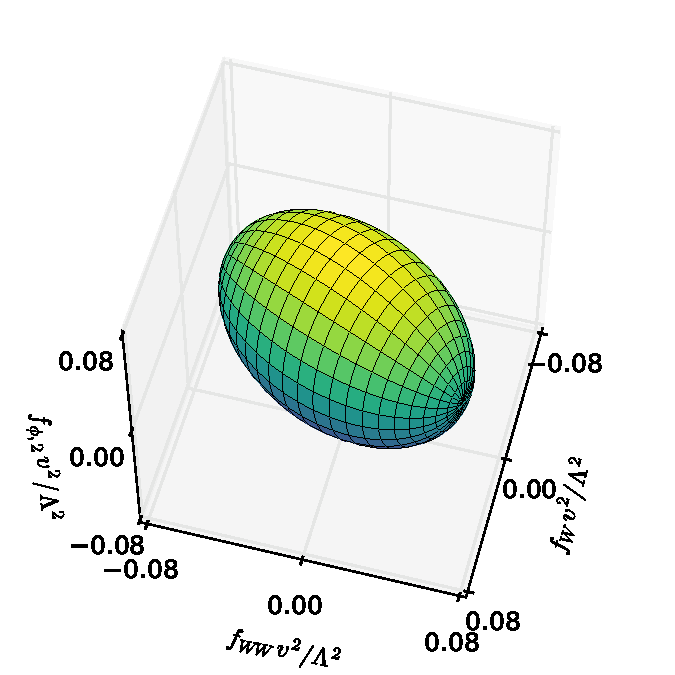
\includegraphics[width=0.49 \textwidth]{fig/information/wbf_tautau_geometry_3d}
  \caption{Error ellipsoid defined by the Fisher information in the
    WBF $h \to \tau \tau$ channel defined by the contour
    $d_\text{local}(\boldtheta ; \boldzero) = 1$. The $\theta_i$ not
    shown are set to zero. }
\label{fig:information_wbf_tautau_geometry_2d}
\end{figure}

These results show that the WBF process has quite different
sensitivities to the five operators: $\ope{\phi,2}$, which is the only
one that affects the decay vertex in addition to the production
process, can be most strongly constrained and is weakly correlated
with $\ope{W}$. An ideal measurement can probe this operator with a
precision of $\Delta \theta \approx 0.02$, translating into a maximal
new physics reach $\Lambda/\sqrt{f_{\phi,2}} \approx 1.9~\tev$. The
sensitivity to the strongly correlated $\ope{W}$-$\ope{WW}$ plane is
also quite large: these directions can be probed at the
$\Delta \theta \approx 0.05$ or
$\Lambda/\sqrt{f_{W/WW}} \approx 1~\tev$ level. Finally, $\ope{B}$ and $\ope{BB}$ only
play a role in subleading $Z$-mediated production diagrams. Their
Wilson coefficients cannot be measured very well in this process, and
does not affect the measurement of the other operators through
correlations.

In \autoref{fig:information_wbf_tautau_geometry_2d} we visualize the
sensitivity to the three operators $\ope{\phi,2}$, $\ope{W}$, and
$\ope{WW}$ as contours of the local information distances from the SM
as defined in \autoref{eq:information_local_distances}. Such an error
ellipsoid shows the maximum precision that can be attained in a
measurement in this process.

\begin{figure}
  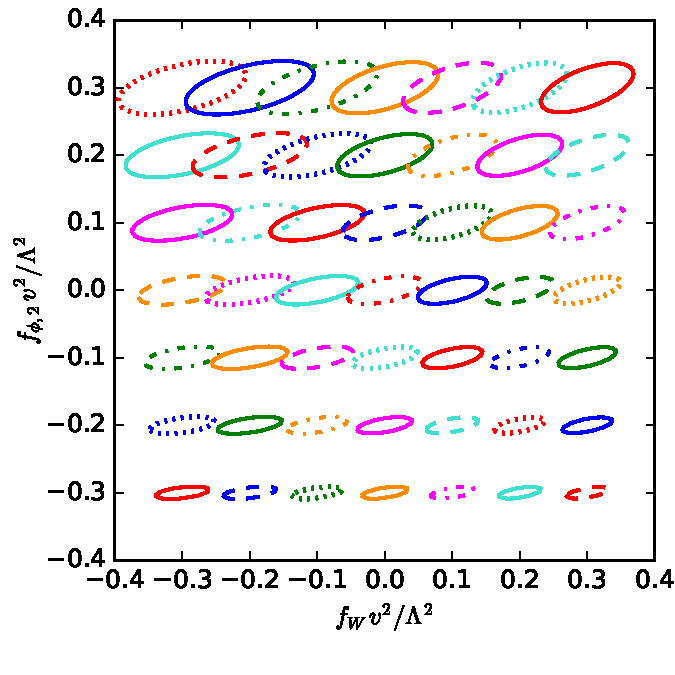
\includegraphics[width=0.33 \textwidth,clip,trim=0.3cm 0 0.05cm 0]{fig/information/wbf_tautau_grid_fphi2_fw}%
  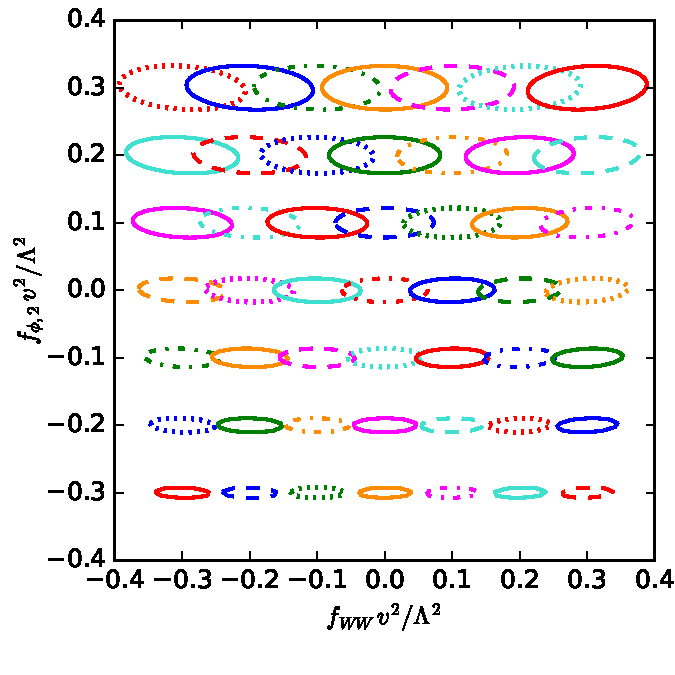
\includegraphics[width=0.33 \textwidth,clip,trim=0.3cm 0 0.05cm 0]{fig/information/wbf_tautau_grid_fphi2_fww}%
  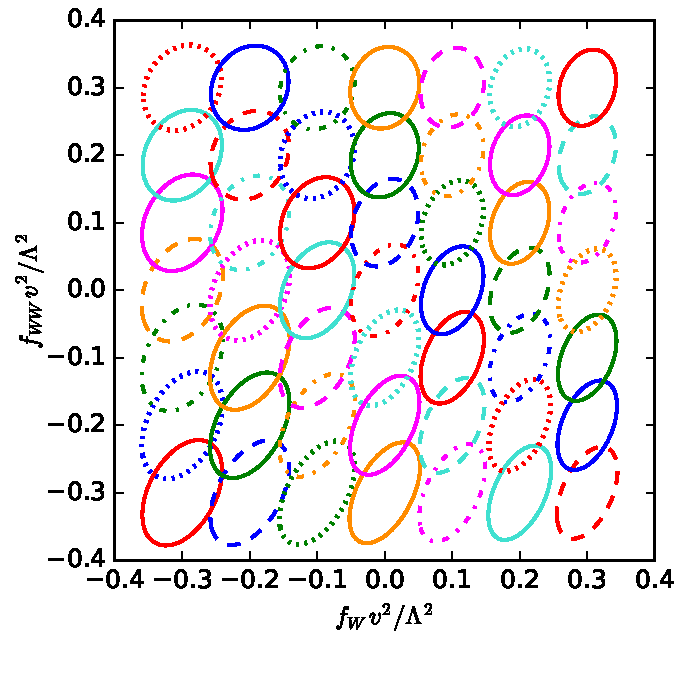
\includegraphics[width=0.33 \textwidth,clip,trim=0.3cm 0 0.05cm 0]{fig/information/wbf_tautau_grid_fww_fw}%
  \caption{Full Fisher information in the WBF $h \to \tau \tau$
    channel at different points in the parameter space. We visualize
    the Fisher information with contours of local distance
    $d_\text{local}(\boldtheta ; \boldtheta_0) = 1$, setting the
    $\theta_i$ not shown to zero. }
\label{fig:information_wbf_tautau_grid}
\end{figure}

Moving away from the SM, the Fisher information and with it the
sensitivity to the different operators changes slightly, see
\autoref{fig:information_wbf_tautau_grid}. The largest change is
visible at large positive (large negative) values of $f_{\phi,2}$,
where the expcted cross section is much smaller (larger) and theory
parameters can be measured with smaller (larger) precision.

Following \autoref{eq:information_global_distances}, we integrate
infinitesimal distances along geodesics in theory space to define
global distances in the model parameter space. Unlike the local
distances, these take into account the curvature of the information
geometry, \ie how the Fisher information changes with the theory
parameters. \autoref{fig:information_wbf_tautau_global_distances} shows the
resulting distances for a number of two-dimensional slices in
parameter space, confirming the large sensitivity to $\ope{\phi2,}$,
$\ope{W}$, and $\ope{WW}$. 

\wbfpyramid{wbf_tautau_global}{fig:information_wbf_tautau_global_distances}
{Error ellipses defined by the Fisher information in the WBF
  $h \to \tau \tau$ channel. We show global distances from the SM
  $d(\boldtheta,\mathbf{0})$, where the $\theta^i$ not shown are set
  to zero. The white contours show distances of $d=1,2,\dots,5$.}

In \autoref{fig:information_wbf_tautau_local_vs_global} we compare the
global distances to the local distances defined in
\autoref{eq:information_local_distances}. This provides some insight
into the role of $\ord{1/\Lambda^4}$ effects, as discussed in
\autoref{sec:information_eft}.  At $d = 1,2$ the differences are
small, signaling that an optimal measurement will be dominated by the
linearized dimension-6 amplitudes. On the other hand, analyses based
on less luminosity or requiring more stringent exclusion criteria
(translating into larger distances) will only probe new physics scales
closer to the electroweak scale, in which case the squared
dimension-six terms will have a larger effect.

\begin{figure}
  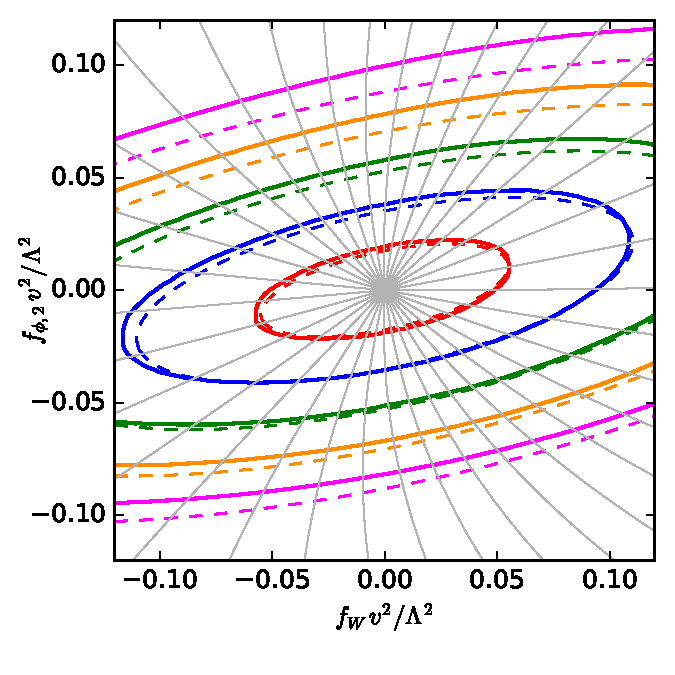
\includegraphics[width=0.33 \textwidth,clip,trim=0.3cm 0 0.05cm 0]{fig/information/wbf_tautau_geometry_fphi2_fw}%
  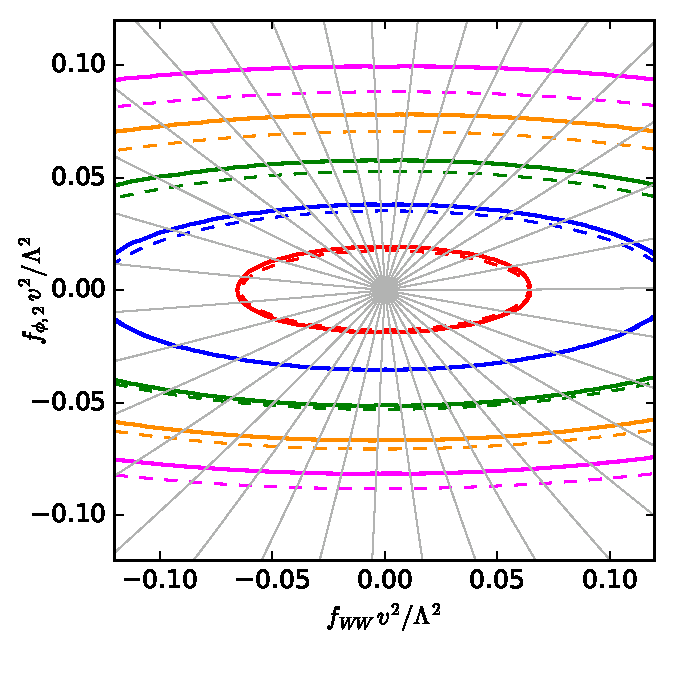
\includegraphics[width=0.33 \textwidth,clip,trim=0.3cm 0 0.05cm 0]{fig/information/wbf_tautau_geometry_fphi2_fww}%
  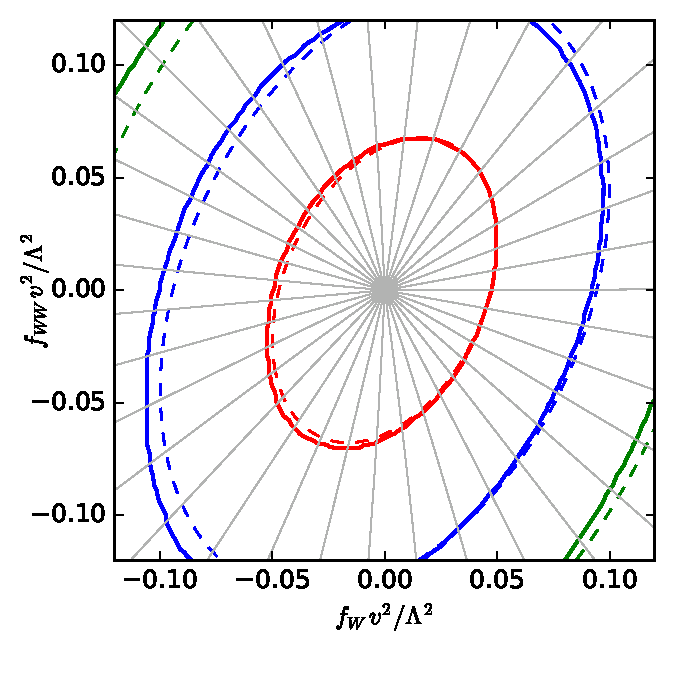
\includegraphics[width=0.33 \textwidth,clip,trim=0.3cm 0 0.05cm 0]{fig/information/wbf_tautau_geometry_fww_fw}%
  \caption{Error ellipses defined by the Fisher information in the WBF
    $h \to \tau \tau$ channel. We show contours of local distance
    $d_\text{local}(\boldtheta ; \boldzero)$ (dashed) and global distance
    $d(\boldtheta,\boldzero)$ (solid).  The colored contours indicate
    distances of $d = 1~...~5$. In grey we show example geodesics. The
    $\theta_i$ not shown are set to zero. }
\label{fig:information_wbf_tautau_local_vs_global}
\end{figure}



%%%%%%%%%%%%%%%%%%%%%%%%%%%%%%%%%%%%%%%%%%%%%%%%%%%%%%%%%%%%
\subsubsection{Differential information}
%%%%%%%%%%%%%%%%%%%%%%%%%%%%%%%%%%%%%%%%%%%%%%%%%%%%%%%%%%%%

In a next step, we calculate the distribution of this information,
evaluated at the SM point $\boldtheta = \boldzero$, over phase
space. In
Figures~\ref{fig:information_wbf_tautau_differential_information_taus}
and \ref{fig:information_wbf_tautau_differential_information_jets} we
show the differential cross sections of the signal and dominant
background process for typical kinematic distributions and compare it
to the differential information.

\begin{figure}
  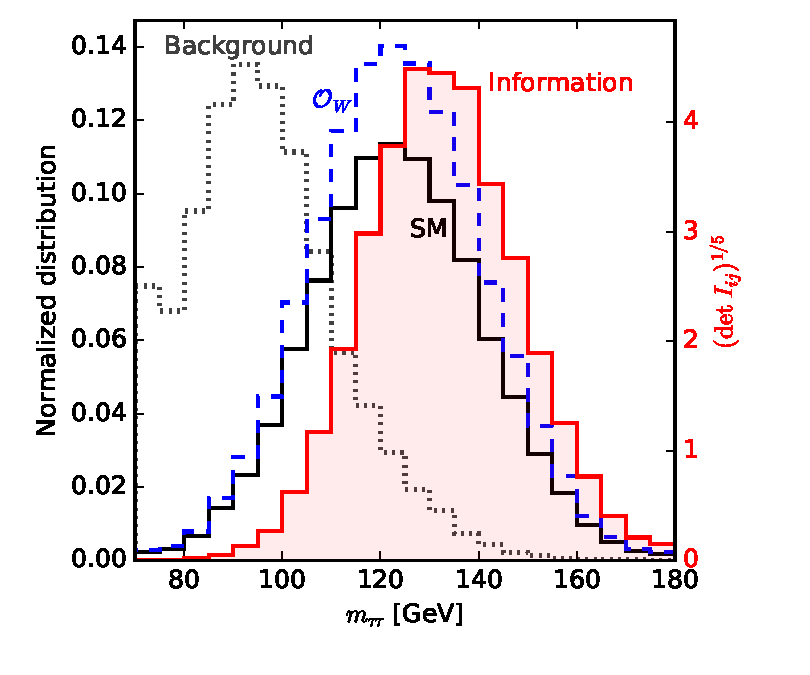
\includegraphics[width=0.49 \textwidth]{fig/information/wbf_tautau_information_over_mtautau}%
  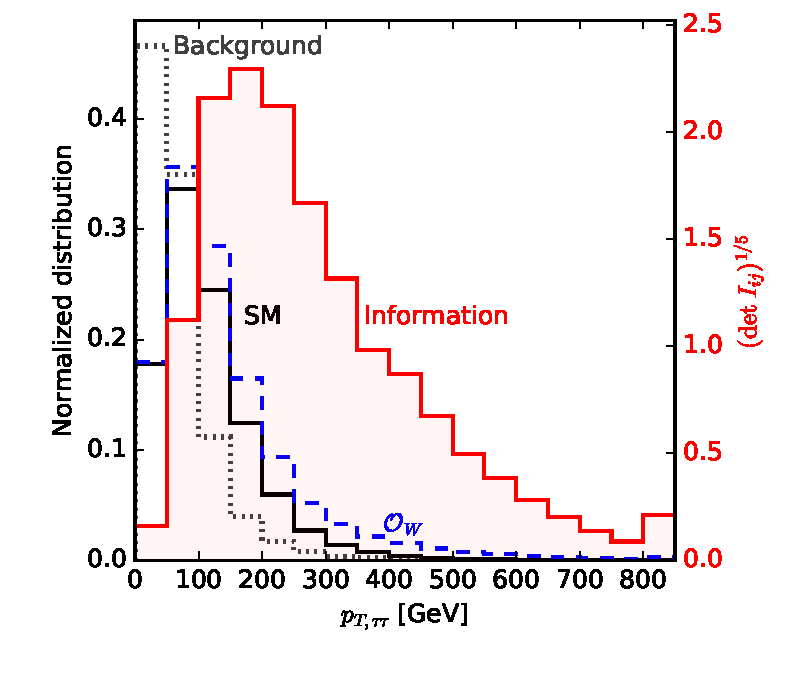
\includegraphics[width=0.49 \textwidth]{fig/information/wbf_tautau_information_over_pttautau}%
  \caption{Distribution of the differential Fisher information in the
    WBF $h \to \tau \tau$ channel (shaded red) with respect to the
    invariant mass of the $\tau \tau$ system (left) and its transverse
    momentum (right). We also show the normalized SM signal (solid
    black) and QCD $Z$+jets (dotted grey) rates. The dashed blue line
    shows the effect of an exaggerated
    $f_{W} \, v^2 / \Lambda^2 = 0.5$. The last bin is an overflow
    bin.}
  \label{fig:information_wbf_tautau_differential_information_taus}
\end{figure}

\begin{figure}
  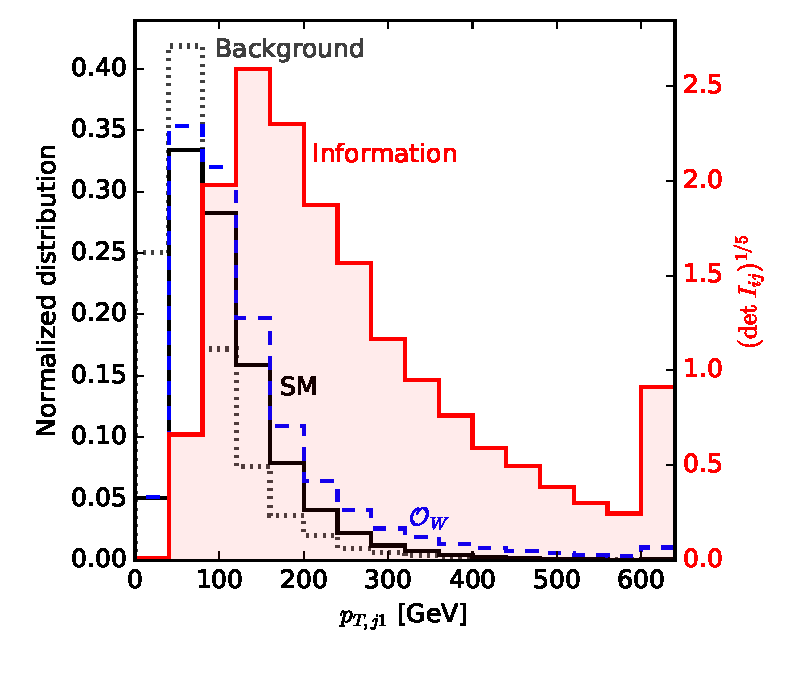
\includegraphics[width=0.49 \textwidth]{fig/information/wbf_tautau_information_over_ptj}%
  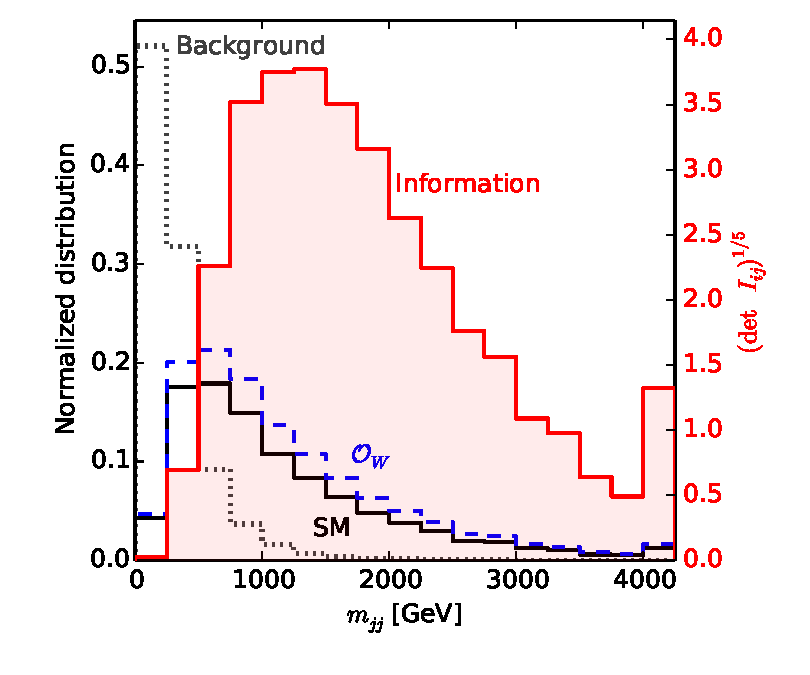
\includegraphics[width=0.49 \textwidth]{fig/information/wbf_tautau_information_over_mjj}\\%
  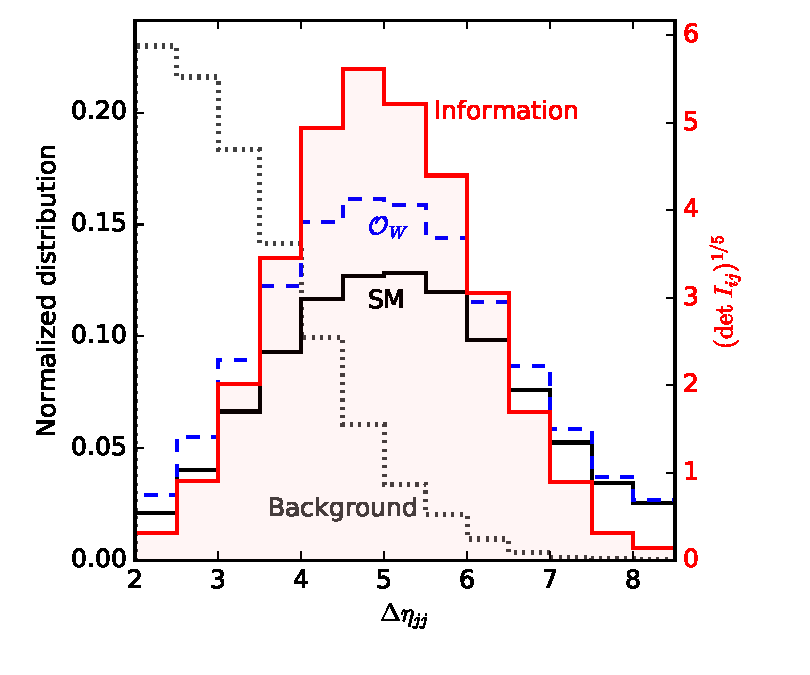
\includegraphics[width=0.49 \textwidth]{fig/information/wbf_tautau_information_over_deltaeta}%
  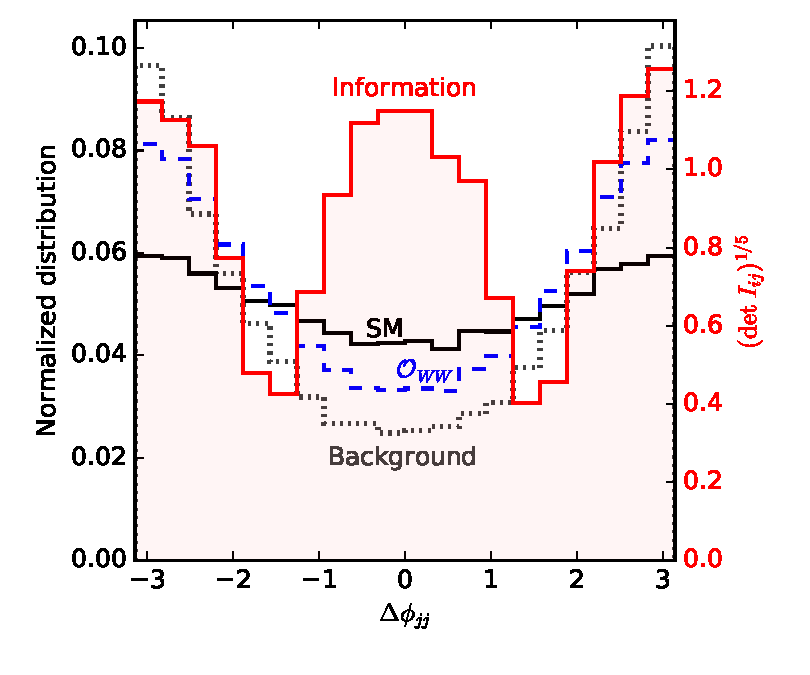
\includegraphics[width=0.49 \textwidth]{fig/information/wbf_tautau_information_over_deltaphi}%
  \caption{Distribution of the differential Fisher information in the
    WBF $h \to \tau \tau$ channel (shaded red) with respect to the
    transverse momentum of the leading jet (top left), the dijet mass
    (top right), the separation in pseudorapidity between the two jets
    (bottom left), and their difference in the azimuthal angle (bottom
    right). We also show the normalized SM signal (solid black) and
    QCD $Z$+jets (dotted grey) rates. The dashed blue line shows the
    effect of an exaggerated $f_{W} \, v^2 / \Lambda^2 = 0.5$, except
    in the bottom right pannel, where we show
    $f_{WW} \, v^2 / \Lambda^2 = 0.5$. The last bin is an overflow
    bin.}
  \label{fig:information_wbf_tautau_differential_information_jets}
\end{figure}

Clearly, the signal-to-background ratio improves for large invariant
masses of the tagging jets and towards $m_{\tau \tau}$ values around
the Higgs mass. The information on all directions in model space is
larger in these phase-space regions. On the other hand, most of our
dimension-six operators include derivatives, leading to an increasing
amplitude with momentum transfer through the gauge-Higgs vertex. This
momentum flow is not observable, but the transverse momenta of the
tagging jets and the Higgs boson are strongly correlated with it, as
shown in \autoref{sec:validity_wbf_observables}. Indeed most of the
information on higher-dimensional operators comes from the high-energy
tail of the transverse momenta of the tagging jets or the $\tau \tau$
system, confirming what we demonstrated for specific model setups in
the previous chapter. Note that these distributions also quantify how
much the power of a Higgs measurement is limited by imposing an upper
limit on the momentum transfer to improve the validity of the EFT.

In the rapidity difference between the tagging jets we can see a
trade-off between these two effects: on the one hand, at larger
rapidity distances the signal-to-background ratio clearly
improves~\cite{Kleiss:1987cj, Baur:1990xe, Barger:1991ib,
  Rainwater:1996ud, Rainwater:1998kj, Cox:2010ug, Gerwick:2011tm}. On
the other hand, the largest effects from dimension-6 operators appear
at smaller $\Delta \eta_{jj}$, again driven by the larger momentum
transfer~\cite{Biekotter:2016ecg}. In the bottom left panel of
\autoref{fig:information_wbf_tautau_differential_information_jets} we
see that most of the information on these operators comes from
$\Delta \eta_{jj} = 3\dots7$. Tight cuts with the aim to remove
backgrounds thus lose a sizable fraction of the information on
dimension-six operators.

In practice, the distribution of the differential information can be a
useful tool to guide the design of event selections. As an example we
consider traditional WBF cuts
%
\begin{equation}
  \Delta \eta_{jj} > \Delta \eta_{jj}^{\text{min}}
  \qquad \text{and} \qquad
  m_{jj} > m_{jj}^{\text{min}} \,.
\end{equation}
%
In \autoref{fig:information_wbf_tautau_cut_scan} we show how the
signal purity and the Fisher information depend on the choice of
$\Delta \eta_{jj}^{\text{min}}$ and $m_{jj}^{\text{min}}$. For a given
signal-to-background ratio we can pick cuts that maximize the Fisher
information, or vice versa, as demonstrated in the left panel of
\autoref{fig:information_wbf_tautau_cut_roc}.  This is somewhat
reminiscent of ``receiver operating characteristic'' (ROC) curves that
compare the efficiency for the SM Higgs signal to the background
rejection rate, as shown in the right panel of
\autoref{fig:information_wbf_tautau_cut_roc}. The information-based
analysis, however, takes into account the sensitivity of signal events
in different phase-space regions to new physics effects, which the ROC
curve is by design blind to.

\begin{figure}
  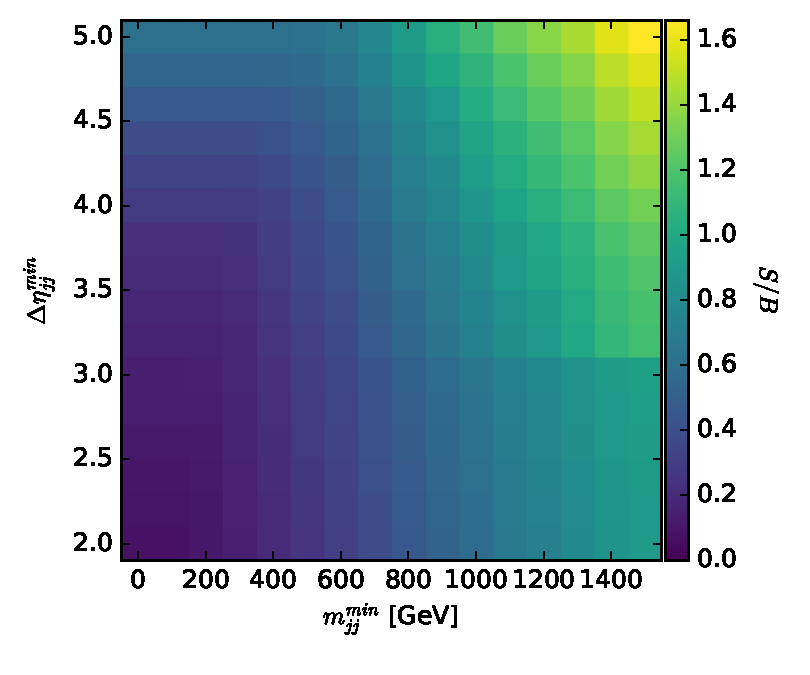
\includegraphics[width=0.49 \textwidth]{fig/information/wbf_tautau_tunecuts_purity}%
  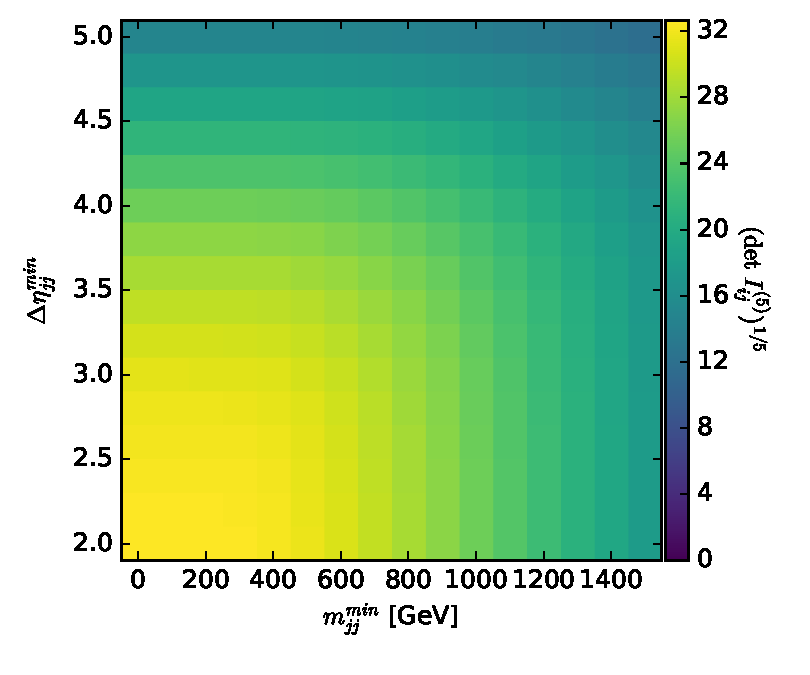
\includegraphics[width=0.49 \textwidth]{fig/information/wbf_tautau_tunecuts_information}%
  \caption{SM signal-to-background ratio (left) and determinant of the
    Fisher information (right) in the WBF $h \to \tau \tau$ channel as
    a function of the WBF cuts
    $\Delta \eta_{jj} > \Delta \eta_{jj}^{\text{min}}$ and
    $m_{jj} > m_{jj}^{\text{min}}$.}
  \label{fig:information_wbf_tautau_cut_scan}
\end{figure}

\begin{figure}
  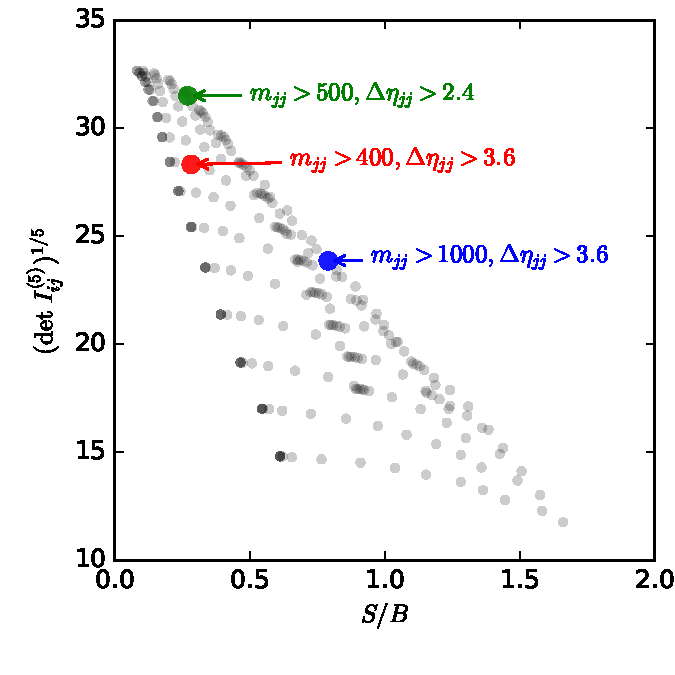
\includegraphics[width=0.49 \textwidth]{fig/information/wbf_tautau_tunecuts_purity_vs_information}%
  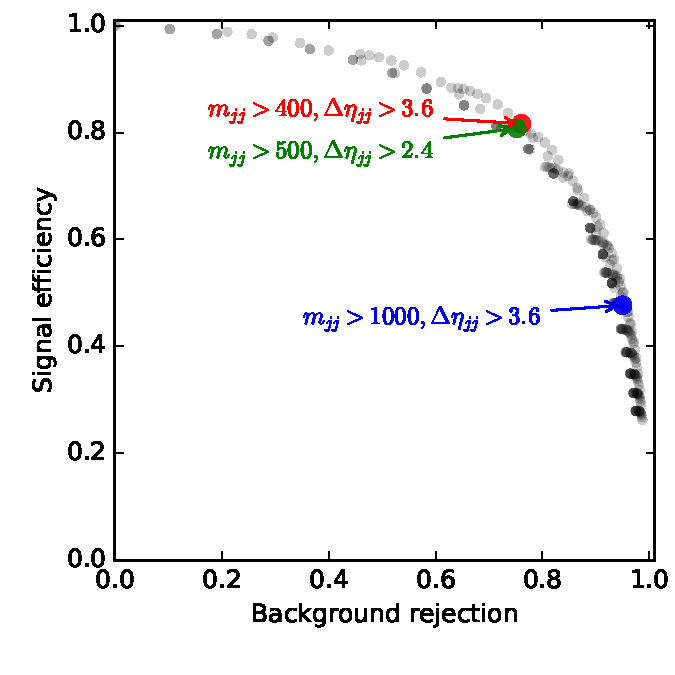
\includegraphics[width=0.49 \textwidth]{fig/information/wbf_tautau_tunecuts_roc}%
  \caption{Trade-off between signal purity and information in the WBF
    $h \to \tau \tau$ channel for different WBF cuts. Left:
    determinant of the Fisher informatiob vs.\ signal-to-background
    ratio. Right: signal efficiency vs.\ background rejection. The
    coloured dots show three examplaric cuts.}
  \label{fig:information_wbf_tautau_cut_roc}
\end{figure}
%
\comment{To here}



%%%%%%%%%%%%%%%%%%%%%%%%%%%%%%%%%%%%%%%%%%%%%%%%%%%%%%%%%%%%
\subsubsection{Information in distributions}
%%%%%%%%%%%%%%%%%%%%%%%%%%%%%%%%%%%%%%%%%%%%%%%%%%%%%%%%%%%%

\begin{figure}
  \includegraphics[width=0.49 \textwidth]{fig/information/wbf_tautau_histos_contours}
  \caption{Information from histograms compared to the full
    information  (black) in the WBF $H \to \tau \tau$ channel, shown as contours
    $d_{\text{local}}(\boldtheta ; \boldzero) = 1$. We include
    $p_{T,j_1}$, $\Delta \phi_{jj}$, their naive combination assuming
    no mutual information, and their two-dimensional histogram. The
    $\theta_i$ not shown are set to zero.}
  \label{fig:information_wbf_tautau_histograms_contours}
\end{figure}

While the integrated, fully differential information defined in
\autoref{eq:information_fisher_rates} provides us with optimal experimental
results, it remains to be shown that we can access it in
practice. Recent proposals using machine learning for high-dimensional
likelihood fits aim to tackle eactly this problem~\cite{machine_learning}.
Regardless, a relevant question is how much of this maximum
information is retained in simple one-dimensional or two-dimensional
distributions of standard kinematic observables $\mathbf{v}$. 

In the presence of backgrounds, a histogram-based analysis first
requires a stringent event selection. We choose the WBF cuts 
%
\begin{align}
  p_{T,j_1} > 50~\gev \qqqquad
  m_{jj} > 1~\tev \qqqquad
  \Delta \eta_{jj} > 3.6 \,.
  \label{eq:information_wbf_tautau_wbfcuts}
\end{align}
%
This improves the signal-to-background ratio to approximately unity,
but at the cost of losing discrimination power. Eventually, a
histogram-based analysis will benefit from optimizing this selection,
for instance foregoing the simple cuts for a multivariate approach,
going beyond the scope of this demonstration.  Based on this
selection, we analyze the distributions
%
\begin{itemize}
\item $p_{T,\tau_1}$ with bin size 25~GeV up to 500~GeV and an
  overflow bin;
\item $m_{\tau \tau}$ with bin size 5~GeV in the allowed range of
  $105~...~165~\gev$.
\item $p_{T,\tau \tau}$ with bin size 50~GeV up to 800~GeV and an
  overflow bin;
\item $p_{T,j_1}$ with bin size 50~GeV up to 800~GeV and an
  overflow bin;
\item $m_{jj}$ with bin size 250~GeV up to 4~TeV and an overflow
  bin;
\item $\Delta \eta_{jj}$ with bin size $0.5$ up to $8.0$ and an
  overflow bin;
\item $\Delta \phi_{jj} = \phi_{j_{\eta < 0}} - \phi_{j_{\eta > 0}}$~\cite{phi_jjs} with bin size $2 \pi / 20$;
\item $\Delta \eta_{\tau\tau, j1}$ with bin size $0.5$ up to $8.0$ and an
  overflow bin;
\item $\Delta \phi_{\tau \tau, j1}$ with bin size $\pi / 10$.
\end{itemize}  

\begin{figure}
  \includegraphics[width=\textwidth]{fig/information/wbf_tautau_histos_comparison}
  \caption{Fisher information for the WBF $H \to \tau \tau$ channel
    exploiting the full phase space, after the cuts in
    \autoref{eq:information_wbf_tautau_wbfcuts}, and for several kinematic
    distributions.  The top panel shows the eigenvalues, the colors
    denote the composition of the corresponding eigenvectors. The
    right axis translates the eigenvalues into a new physics reach for
    the corresponding combination of Wilson coefficients.  In the
    bottom panel we show the determinants of the Fisher information
    restricted to $\ope{\phi,2}$, $\ope{W}$, and $\ope{WW}$,
    normalized to the full information. Again, the right axis
    translates them into a new physics reach.}
\label{fig:information_wbf_tautau_histograms_comparison}
\end{figure}

\autoref{fig:information_wbf_tautau_histograms_contours} demonstrates that
virtuality measures such as the transverse momentum of the leading
tagging jet mostly constrain $\ope{W}$, while angular correlations
between the jets are more sensitive to $\ope{WW}$. Stringent
constraints on the full operator space can only be achieved by
combining the information in these distributions, ideally in a
two-dimensional histogram.

In \autoref{fig:information_wbf_tautau_histograms_comparison} we extend our
comparison to the information in all of the above distributions. The
top panel shows the eigenvalues of the individual information
matrices, and the colors indicate which operators the corresponding
eigenvectors are composed of. This allows us to see which operators
can be measured well in which distributions, and where blind (or flat)
directions arise. In the lower panel we compare the determinants,
providing a straightforward measure of the information in
distributions that is invariant under basis rotations. 

In general, single differential cross sections probe individual
directions in phase space well, but always suffer from basically blind
directions. To maximize the constraining power on all operators we
need to combine virtuality measures and angular correlations. Even
then there is a substantial difference to the maximum information in
the process: the combined analysis of jet transverse momenta and
$\Delta \phi_{jj}$ has a new physics reach in the
$\ope{\phi,2}$-$\ope{W}$-$\ope{WW}$ space of $0.9~\tev$, compared to
$1.2~\tev$ for the fully differential cross section.  Under our
simplistic assumptions this corresponds to roughly three times more
data.  Half of this loss in constraining power is due to information
in background-rich regions discarded by the WBF cuts, and half is due
to non-trivial kinematics not captured by the double differential
distributions.
%
\comment{To here on Thursday}




%%%%%%%%%%%%%%%%%%%%%%%%%%%%%%%%%%%%%%%%%%%%%%%%%%%%%%%%%%%%
\subsection{Weak-boson-fusion Higgs to four leptons}
\label{sec:information_wbf_4l}
%%%%%%%%%%%%%%%%%%%%%%%%%%%%%%%%%%%%%%%%%%%%%%%%%%%%%%%%%%%%

Another question we can approach with information geometry is how much
the non-trivial decay mode $H \to 4 \ell$ adds to the WBF production
analyzed in \autoref{sec:information_wbf_taus}. For this particularly clean
channel, shown in \autoref{fig:information_wbf_4l_diag}, the backgrounds are
not the limiting factor, so we omit them for our toy study. This also 
allows us to avoid smearing the $m_{4\ell}$ distribution. At parton
level we apply the generator-level cuts
%
\begin{alignat}{2}
  p_{T,j} &> 20 \ \gev \qquad & \qquad |\eta_{j}| &< 5.0  \notag \\ 
  p_{T,\ell} &> 10 \ \gev  \qquad & \qquad |\eta_{\ell}| &< 2.5 \; ,
\label{eq:information_wbf_4l_acceptance_cuts}
\end{alignat}
%
with $\ell = e, \mu$. The SM cross section after these cuts is 0.36~fb.



%%%%%%%%%%%%%%%%%%%%%%%%%%%%%%%%%%%%%%%%%%%%%%%%%%%%%%%%%%%%
\subsubsection*{Maximum precision on Wilson coefficients}
%%%%%%%%%%%%%%%%%%%%%%%%%%%%%%%%%%%%%%%%%%%%%%%%%%%%%%%%%%%%

Again we study the five-dimensional space of CP-even Wilson
coefficients given in \autoref{eq:information_wilson_space_wbf}.  For increased
luminosity, $L \cdot \varepsilon = 100~\ifb$, we find the SM
information
%
\begin{align}
  I_{ij} (\boldzero) =
\begin{pmatrix*}[r]
  144.3 & -27.3 & -11.5 & -1.6 & -0.7 \\
  -27.3 & 50.9 & -9.1 & 6.7 & -0.2 \\
  -11.5 & -9.1 & 36.9 & -1.2 & 1.0 \\
  -1.6 & 6.7 & -1.2 & 1.9 & -0.1 \\
  -0.7 & -0.2 & 1.0 & -0.1 & 0.1
\end{pmatrix*}
\end{align}
%
with the eigenvectors 
%
\begin{align}
  \boldtheta_1 = \fivevecr {0.96} {-0.25} {-0.08} {-0.02} {0.00}  \qquad 
  \boldtheta_2 = \fivevecr {-0.16} {-0.79} {0.58} {-0.11} {0.02}  \qquad
  \boldtheta_3 = \fivevecr {0.21} {0.54} {0.81} {0.09} {0.02} \qquad 
  \boldtheta_4 = \fivevecr {0.02} {0.14} {0.01} {-0.99} {0.04}  \qquad 
  \boldtheta_5 = \fivevecr {0.00} {-0.00} {-0.03} {0.04} {1.00}  \,.
\end{align}
%
and the eigenvalues $\left( 152.4, 52.8, 27.8, 1.0, 0.0 \right)$. 

When we compare the above outcome to our earlier WBF production analysis we see
that the decay $H \to 4\ell$ does not increase the sensitivity to
$\ope{B}$ or $\ope{BB}$; both of them are still basically blind
directions. We visualize the information geometry in the remaining
directions in \autoref{fig:information_wbf_4l_geometry}. The differences between
local and global distances are much larger than in the $H \to \tau
\tau$ channel. This is because the tiny $H \to 4\ell$ branching
fraction decreases the new physics reach and with it the hierarchy of
scales in our effective Lagrangian. This means that the squared
dimension-6 amplitudes are numerically more relevant.

\begin{figure}
  \includegraphics[width=0.33 \textwidth,clip,trim=0.3cm 0 0.05cm 0]{fig/information/wbf_4l_geometry_fphi2_fw}%
  \includegraphics[width=0.33 \textwidth,clip,trim=0.3cm 0 0.05cm 0]{fig/information/wbf_4l_geometry_fphi2_fww}%
  \includegraphics[width=0.33 \textwidth,clip,trim=0.3cm 0 0.05cm 0]{fig/information/wbf_4l_geometry_fww_fw}%
  \caption{Error ellipses defined by the Fisher information in the
    WBF $H \to 4\ell$ channel. We show contours of local distance
    $d_\text{local}(\boldtheta ; \boldzero)$ (dashed) and global
    distance $d(\boldtheta,\boldzero)$ (solid). The colored contours
    indicate distances of $d = 1~...~5$. In grey we show example
    geodesics.  The $\theta_i$ not shown are set to zero.}
\label{fig:information_wbf_4l_geometry}
\end{figure}



%%%%%%%%%%%%%%%%%%%%%%%%%%%%%%%%%%%%%%%%%%%%%%%%%%%%%%%%%%%%
\subsubsection*{Production vs decay kinematics}
%%%%%%%%%%%%%%%%%%%%%%%%%%%%%%%%%%%%%%%%%%%%%%%%%%%%%%%%%%%%

\begin{figure}
  \includegraphics[width=0.49 \textwidth]{fig/information/wbf_4l_production_decay_fphi2_fww}
  \caption{Information in the WBF $H \to 4\ell$ channel from including
    dimension-6 operators only in the production vertex (red), only in
    the decay vertex (blue), and both (black). The information is
    visualized as local contours
    $d_{\text{local}}(\boldtheta ; \boldzero) = 1$. The $\theta_i$ not shown
    are set to zero.}
\label{fig:information_wbf_4l_production_decay}
\end{figure}

Focusing on the question how the decay analysis improves our global
information, we disentangle the effects on the production and decay
vertices in \autoref{fig:information_wbf_4l_production_decay}.  As well known for
the LHC, the production-side analysis benefits from a large momentum
flow through the Higgs vertex, while the momentum flow through the
decay vertices is bounded by the Higgs mass (neglecting off-shell
phase space regions).  For momentum-dependent operators this
disadvantage is not compensated by the complex $H \to 4\ell$ decay
kinematics.  Consequently, the Higgs decay only improves the reach in
the $\ope{\phi,2}$ direction, corresponding to a change in the total rate. 
This operator also affects many other total Higgs rates,
so we conclude that the complex $H \to 4\ell$ kinematics
does not play a significant role as part of a global analysis. 

\begin{figure}
  \includegraphics[width= \textwidth]{fig/information/wbf_4l_histos_comparison}
  \caption{Fisher information for the WBF $H \to 4 \ell$ channel
    exploiting the full phase space, after the cuts in
    \autoref{eq:information_wbf_tautau_wbfcuts}, and for several kinematic
    distributions.  The top panel shows the eigenvalues, the colors
    denote the composition of the corresponding eigenvectors. The
    right axis translates the eigenvalues into a new physics reach for
    the corresponding combination of Wilson coefficients.  In the
    bottom panel we show the determinants of the Fisher information
    restricted to $\ope{\phi,2}$, $\ope{W}$, and $\ope{WW}$,
    normalized to the full information. Again, the right axis
    translates them into a new physics reach.}
\label{fig:information_wbf_4l_histograms_comparison}
\end{figure}

In complete analogy to \autoref{fig:information_wbf_tautau_histograms_comparison}
for the WBF production, we compare the information in different
distributions for $CP$-even operators in
\autoref{fig:information_wbf_4l_histograms_comparison}.  The standard tagging jet
observables are complemented by five observables characterizing the
$4\ell$ decay kinematics,
%
\begin{itemize}
  \item $p_{T,\ell_1}$;
  \item $p_{T,4\ell}$;
  \item $m_{Z_2}$ for the lower-mass reconstructed $Z$ boson;
  \item $\cos \theta_1 = \hat{p}_{\ell^-_1} \cdot \hat{p}_{Z_2}
    \Big|_{Z_1}$ defined in terms of unit-3-vectors $\hat{p}$, and analogously
    $\cos \theta_2^*$;
  \item $\cos \Phi = ( \hat{p}_{\ell^-_1} \times
    \hat{p}_{\ell^+_1} ) \cdot ( \hat{p}_{\ell^-_2} \times
    \hat{p}_{\ell^+_2} )$, defined in the $ZZ$ or Higgs rest
    frame~\cite{phi_jj}.
\end{itemize}
%
In all cases we use at least ten bins and include underflow and
overflow bins where applicable.

In our quantitative analysis we find similar patterns as in the
$\tau \tau$ mode. The key observables are again transverse momenta and
jet angular correlations. Without the complication of removing
backgrounds efficiently, the combined analysis of these variables
comes close to the maximum information: a two-dimensional histogram of
jet transverse momenta and $\Delta \phi_{jj}$ probes new physics
scales up to 650~GeV, while for a fully differential analysis the
maximum probed new physics scale is close to 700~GeV. Under our
assumptions, this difference roughly corresponds to 25\% more
data. The decay kinematics and its angular observables do not help
significantly or change the picture qualitatively.  This shows again
how much the sensitivity of the decay vertices to dimension-6
operators is limited by the restriction of the momentum flow to the
Higgs mass. This is not accidental: the reason behind this role of the
momentum dependence is that for all operators shown in
\autoref{eq:information_wilson_space_wbf} with the exception of $\ope{\phi,2}$,
gauge invariance forces us to include the field strength tensor
instead of the gauge boson field, automatically introducing a momentum
dependence.



%%%%%%%%%%%%%%%%%%%%%%%%%%%%%%%%%%%%%%%%%%%%%%%%%%%%%%%%%%%%
\subsection{Higgs plus single top}
\label{sec:information_th}
%%%%%%%%%%%%%%%%%%%%%%%%%%%%%%%%%%%%%%%%%%%%%%%%%%%%%%%%%%%%

Our final example is Higgs production with a single top with
$H\to \gamma \gamma$ and a hadronic top decay. As shown in
\autoref{fig:information_th_diag}, diagrams where the Higgs is
radiated off a $W$ boson interfere destructively with diagrams with a
top-Higgs coupling, making this channel a direct probe of the sign of
the top Yukawa coupling~\cite{top_higgs}. We stick to a parton-level
analysis at leading order in the five-flavor scheme. For our toy
example we include only one of the dominant backgrounds, single top
production with two photons, and in particular ignore the multi-jet
background. The subleading $t\bar{t} \, \gamma\gamma$ background
populates qualitatively different phase-space regions from the
single-top signal and can be supressed with an appropriate event
selection~\cite{Kling:2012up}. We smear the $m_{\gamma \gamma}$
distribution of the signal process with a Gaussian of width 1.52 GeV
estimated from Figure~6b of Reference~\cite{CMS:2016zjv}, and do not
include any other detector effects. Our basic event selection requires
%
\begin{alignat}{4}
  p_{T,j} &> 20 \ \gev \quad & \quad
  |\eta_{j}| &< 5.0 \quad & \quad
  \Delta R_{jj} &> 0.4 \quad & \quad
  152 \ \gev &<m_{bjj} < 192 \ \gev \notag \\ 
  p_{T,\gamma} &> 10 \ \gev \quad & \quad
  |\eta_{\gamma}| &< 2.5 \quad & \quad 
  \Delta R_{\gamma j} , \Delta R_{\gamma \gamma} &> 0.4 \quad & \quad
  120 \ \gev &<m_{\gamma \gamma} < 130 \ \gev \,,
  \label{eq:information_th_acceptance_cuts}
\end{alignat}
%
leading to a SM $tH$ cross section of 0.10~fb and a background of 0.22~fb.

We consider four $CP$-even dimension-6 operators
%
\begin{alignat}{2}
  \ope{W}  &= i \frac{g}{2} \, (D^\mu\phi)^\dagger \sigma^k ( D^\nu\phi) \, W_{\mu\nu}^k  \qquad & \qquad
  \ope{t \phi}  &= (\phisq) \, ( \overbar{Q}_3 \tilde{\phi} t_R)  + \text{h.c.} \notag \\
  \ope{WW}  &= -\frac{g^2}{4} \, (\phisq) \, W^k_{\mu\nu} \, W^{\mu\nu\, k}  \qquad & \qquad
  \ope{\phi,2}  &= \frac{1}{2} \, \partial^\mu(\phi^\dagger\phi) \, \partial_\mu(\phi^\dagger\phi) \,.
\label{eq:information_th_ope}
\end{alignat}
%
The operators $\ope{W}$ and $\ope{WW}$ affect the production amplitudes where
the Higgs couples to a $W$, while $\ope{t \phi}$ re-scales the top
Yukawa coupling. Both, $\ope{WW}$ and $\ope{\phi,2}$ also affect the
$H \to \gamma \gamma$ decay.


%%%%%%%%%%%%%%%%%%%%%%%%%%%%%%%%%%%%%%%%%%%%%%%%%%%%%%%%%%%%
\subsubsection*{Maximum precision on Wilson coefficients}
%%%%%%%%%%%%%%%%%%%%%%%%%%%%%%%%%%%%%%%%%%%%%%%%%%%%%%%%%%%%

\begin{figure}
  \includegraphics[width=0.33 \textwidth,clip,trim=0.3cm 0 0.05cm 0]{fig/information/th_geometry_fphi2_fw}%
  \includegraphics[width=0.33 \textwidth,clip,trim=0.3cm 0 0.05cm 0]{fig/information/th_geometry_fphi2_ftphi}%
  \includegraphics[width=0.33 \textwidth,clip,trim=0.3cm 0 0.05cm 0]{fig/information/th_geometry_ftphi_fw}%
  \caption{Error ellipses defined by the Fisher information in Higgs
    plus single top production. We show contours of local distance
    $d_\text{local}(\boldtheta ; \boldzero)$ (dashed) and global distance
    $d(\boldtheta,\boldzero)$ (solid).  The colored contours indicate
    distances of $d = 1~...~5$. In grey we show example geodesics. The
    $\theta_i$ not shown are set to zero. }
\label{fig:information_th_geometry}
\end{figure}


We calculate the Fisher information in terms of the dimensionless parameters
%
\begin{align}
  \boldtheta = \frac {v^2} {\Lambda^2}  \fourvec {f_{\phi,2}} {f_W} {f_{WW}} {f_{t \phi}}
  \label{eq:information_wilson_space_th}
\end{align}
%
for 13~TeV and an integrated luminosity times efficiencies of
$L \cdot \varepsilon = 300~\ifb$ and find
%
\begin{align}
  I_{ij} (\mathbf{0}) =
\begin{pmatrix*}[r]
  80.1 & -18.7 & -957.0 & 13.2 \\
  -18.7 & 32.6 & 221.7 & 27.0 \\
  -957.0 & 221.7 & 11446.1 & -146.0 \\
  13.2 & 27.0 & -146.0 & 150.3
\end{pmatrix*} \, .
\end{align}
%
The eigenvectors are
%
\begin{align}
  \boldtheta_1 = \fourvecr {0.08} {-0.02} {-1.00} {0.01}  \qquad 
  \boldtheta_2 = \fourvecr {0.00} {-0.23} {-0.01} {-0.97} \qquad 
  \boldtheta_3 = \fourvecr {-0.02} {0.97} {-0.02} {-0.23} \qquad 
  \boldtheta_4 = \fourvecr {1.00} {0.02} {0.08} {-0.01}
\end{align}
%
with corresponding eigenvalues $\left( 11532, 155, 21.3, 0.1 \right)$.
The best constrained direction along $\ope{WW}$ corresponds to the
combination of Wilson coefficients that affects the
$H \to \gamma \gamma$ decay in addition to production effects, which
will already be tightly constrained once a $tH$ measurement is
feasible. The orthogonal direction in the $\ope{\phi,2}$-$\ope{W}$
plane is for all practical purposes blind. Even with the assumed
sizeable event rate corresponding to 300~$\ifb$, the sensitivity to
$\ope{W}$ and $\ope{t \phi}$ is limited, with some mixing between the
two operators.

We visualize this maximum sensitivity to dimension-6 operators in
\autoref{fig:information_th_geometry}. With the exception of $\ope{WW}$, an
optimal measurement can probe all operators at the
$\Delta g \approx 0.1\dots 0.2$ level, equivalent to
$\Lambda/\sqrt{f_{\phi,2}} \approx 600 \dots 750$~GeV.  There are
large differences between local and global distances already at the
$d = 2$ level, implying that a measurement of this channel will always
be sensitive to the squared dimension-6 terms.



%%%%%%%%%%%%%%%%%%%%%%%%%%%%%%%%%%%%%%%%%%%%%%%%%%%%%%%%%%%%
\subsubsection*{Differential information}
%%%%%%%%%%%%%%%%%%%%%%%%%%%%%%%%%%%%%%%%%%%%%%%%%%%%%%%%%%%%

\begin{figure}
  \includegraphics[width=0.49 \textwidth]{fig/information/th_information_over_ptaa}%
  \includegraphics[width=0.49 \textwidth]{fig/information/th_information_over_deltaeta}%
  \caption{Distribution of the Fisher information in the Higgs plus
    single top channel (shaded red). We also show the normalized SM
    signal (solid black) and single-top background (dotted grey)
    rates. The dashed blue line shows the effect of
    $f_{t \phi} \, v^2 / \Lambda^2 = 0.2$. The last bin is an overflow
    bin.}
  \label{fig:information_th_differential_information}
\end{figure}

In \autoref{fig:information_th_differential_information} we show the distribution
of this information over phase space. More distributions are shown in
Appendix~\ref{sec:information_additional_plots}. As expected, the information is
concentrated in the $m_{\gamma \gamma} \sim m_H$ peak and in the
high-energy tails of transverse momenta. Studying angular correlations
between the Higgs system and the top decay products, we find that the
region $\Delta \eta_{ \gamma \gamma, bjj} \lesssim 3$ contains a lot
of discrimination power.




%%%%%%%%%%%%%%%%%%%%%%%%%%%%%%%%%%%%%%%%%%%%%%%%%%%%%%%%%%%%
\subsubsection*{Information in distributions}
%%%%%%%%%%%%%%%%%%%%%%%%%%%%%%%%%%%%%%%%%%%%%%%%%%%%%%%%%%%%

In a next step, we compare this full information to the reduced
information in one-dimensional and two-dimensional distributions of
kinematic observables. We now require harder cuts
%
\begin{align}
  p_{T,j_1} > 50~\gev \qquad 
  p_{T,\gamma} > 50,~30~\gev \qquad
  122~\gev < m_{\gamma \gamma} < 128~\gev \,,
  \label{eq:information_th_cuts}
\end{align}
%
which reduces the background to the level of the signal. We then
analyze the distributions~\cite{top_higgs,Kling:2012up}
%
\begin{itemize}
\item $p_{T,\gamma_1}$ with bin size 25~GeV up to 400~GeV and an
  overflow bin;
\item $m_{\gamma\gamma}$ with bin size 1~GeV in the allowed range of
  $123~...~127~\gev$;
\item $p_{T,\gamma \gamma}$ with bin size 40~GeV up to 600~GeV and an
  overflow bin;
\item $\Delta \phi_{\gamma \gamma}$ with bin size $\pi/10$;  
\item $p_{T,j_1}$ with bin size 40~GeV up to 400~GeV and an
  overflow bin;
\item $p_{T,b}$ with bin size 40~GeV up to 400~GeV and an
  overflow bin;
\item $p_{T,bjj}$ with bin size 40~GeV up to 600~GeV and an
  overflow bin;
\item $\Delta \phi_{\gamma \gamma, b}$ with bin size $\pi / 10$;
\item $\Delta \eta_{\gamma\gamma, b}$ with bin size $0.5$ up to $5.0$ and an
  overflow bin;
\item $m_{\gamma \gamma bjj}$ with bin size 100~GeV up to 1500~GeV and an
  overflow bin;
\item $p_{T,\gamma \gamma bjj}$ with bin size 40~GeV up to 400~GeV and an
  overflow bin;
\item $\Delta \phi_{\gamma \gamma, bjj}$ with bin size $\pi / 10$;
\item $\Delta \eta_{\gamma\gamma, bjj}$ with bin size $0.5$ up to $5.0$ and an
  overflow bin.
\end{itemize} 

\begin{figure}
  \includegraphics[width=0.49 \textwidth]{fig/information/th_histos_contours}
  \caption{Information from histograms compared to the full
    information (black), shown as contours
    $d_{\text{local}}(\boldtheta ; \boldzero) = 1$. We include
    $p_{T,\gamma \gamma}$, $\Delta \eta_{\gamma\gamma, bjj}$, their naive combination assuming
    no mutual information, and their two-dimensional histogram. The
    $\theta_i$ not shown are set to zero.}
  \label{fig:information_th_histograms_contours}
\end{figure}

As in the WBF case, different observables probe different Wilson
operators. \autoref{fig:information_wbf_tautau_histograms_contours} shows that
the di-photon transverse momentum constrains mostly the $\ope{W}$
direction, while the rapidity separation between the Higgs and top
systems is more sensitive to $\ope{t\phi}$.

\begin{figure}
  \includegraphics[width= \textwidth]{fig/information/th_histos_comparison}
  \caption{Fisher information for the Higgs plus single top channel
    exploiting the full phase space, after the cuts in
    \autoref{eq:information_th_cuts}, and for several kinematic distributions.
    The top panel shows the eigenvalues, the colors denote the
    composition of the corresponding eigenvectors. The right axis
    translates the eigenvalues into a new physics reach for the
    corresponding combination of Wilson coefficients.  In the bottom
    panel we show the determinants of the Fisher information
    restricted to $\ope{\phi,2}$, $\ope{W}$, and $\ope{t\phi}$,
    normalized to the full information. Again, the right axis
    translates them into a new physics reach.}
\label{fig:information_th_histograms_comparison}
\end{figure}

In \autoref{fig:information_th_histograms_comparison} we compare the eigenvalues,
eigenvectors and determinants of the information matrices in all of
the above distributions. We confirm that the photon observables mostly
probe changes in the Higgs-gauge coupling from $\ope{W}$, while a
rescaled top Yukawa will be visible in the properties of the top decay
products. Distributions of the properties of the $b$ jet consistently
contain significantly less information than the corresponding
distributions for the reconstructed top system. The rapidity
difference between the $\gamma \gamma$ system and the reconstructed
top provides a particularly good probe of this
operator~\cite{top_higgs}. Combining this variable with the transverse
momentum of the $\gamma \gamma$ system we can probe new physics scales
in the $\ope{W}$-$\ope{t\phi}$ plane around 550~GeV in the
$\ope{W}$-$\ope{WW}$-$\ope{\phi,2}$ space, compared to 700~GeV for the
fully differential cross section. This corresponds to almost three
times more data under our simplifying assumptions. 
%
\comment{To here on Friday}



%%%%%%%%%%%%%%%%%%%%%%%%%%%%%%%%%%%%%%%%%%%%%%%%%%%%%%%%%%%%
\section{$CP$ violation in the Higgs sector}
\label{sec:information_application_odd}
%%%%%%%%%%%%%%%%%%%%%%%%%%%%%%%%%%%%%%%%%%%%%%%%%%%%%%%%%%%%




%%%%%%%%%%%%%%%%%%%%%%%%%%%%%%%%%%%%%%%%%%%%%%%%%%%%%%%%%%%%
\section{Technical questions}
\label{sec:information_extensions}
%%%%%%%%%%%%%%%%%%%%%%%%%%%%%%%%%%%%%%%%%%%%%%%%%%%%%%%%%%%%

%%%%%%%%%%%%%%%%%%%%%%%%%%%%%%%%%%%%%%%%%%%%%%%%%%%%%%%%%%%%
\subsection{Systematic uncertainties}
 %%%%%%%%%%%%%%%%%%%%%%%%%%%%%%%%%%%%%%%%%%%%%%%%%%%%%%%%%%%%

\begin{figure}
  \includegraphics[width=0.49 \textwidth]{fig/information/wbf_tautau_systematics_nuisance.pdf}%
  \includegraphics[width=0.49 \textwidth]{fig/information/wbf_tautau_systematics_profiled.pdf}%
  \caption{Effects of Gaussian uncertainties of $5\%$ and $10\%$ on
    the total signal rate. In the left panel we show the expected
    error ellipse $d_{\text{local}}( (g,\nu) ; \boldzero) = 1$ in
    the plane spanned by a physical parameter and the nuisance
    parameter $\nu$ rescaling the signal rate. In the right panel we
    show the error ellipses in the $\ope{W}$-$\ope{\phi,2}$ plane
    after profiling over this systematic uncertainty.}
  \label{fig:information_wbf_tautau_systematics}
\end{figure}

\begin{figure}
  \includegraphics[width= \textwidth]{fig/information/wbf_tautau_histos_comparison_systematics.pdf}
  \caption{Fisher information for the WBF $H \to \tau \tau$ channel
    profiled over a $10\%$ signal rate uncertainty. We compare the
    information for the full phase space, after the cuts in
    \autoref{eq:information_wbf_tautau_wbfcuts}, and for several kinematic
    distributions.  The top panel shows the eigenvalues, the colors
    denote the composition of the corresponding eigenvectors. The
    right axis translates the eigenvalues into a new physics reach for
    the corresponding combination of Wilson coefficients.  In the
    bottom panel we show the determinants of the Fisher information
    restricted to $\ope{\phi,2}$, $\ope{W}$, and $\ope{WW}$,
    normalized to the full information. Again, the right axis
    translates them into a new physics reach.}
  \label{fig:information_wbf_tautau_systematics_comparison}
\end{figure}

We demonstrate this for WBF Higgs production in the $\tau \tau$ mode
in \autoref{fig:wbf_tautau_systematics}. We assign a $5\%$ or $10\%$
Gaussian uncertainty on the overall signal rate, representing for
instance missing higher orders, pdf or efficiency uncertainties. This
significantly reduces the information in the total rate, and thus
mostly the expected precision in the $\ope{\phi,2}$ direction.  In
\autoref{fig:wbf_tautau_systematics_comparison} we show how the
information in various distributions is affected by such an
uncertainty. The new physics reach in the $\ope{\phi,2}$ direction is
reduced by 800~GeV. 




%%%%%%%%%%%%%%%%%%%%%%%%%%%%%%%%%%%%%%%%%%%%%%%%%%%%%%%%%%%%
\subsection{Comparison with other tools}
%%%%%%%%%%%%%%%%%%%%%%%%%%%%%%%%%%%%%%%%%%%%%%%%%%%%%%%%%%%%

%%%%%%%%%%%%%%%%%%%%%%%%%%%%%%%%%%%%%%%%%%%%%%%%%%%%%%%%%%%%
\subsubsection*{Likelihood ratio}
%%%%%%%%%%%%%%%%%%%%%%%%%%%%%%%%%%%%%%%%%%%%%%%%%%%%%%%%%%%%

There is some subtlety in the relationship between 
standard likelihood ratio tests and the Fisher distance.
We anticipate that the confidence intervals in $\boldtheta$ will continue 
to be based on likelihood ratio tests.
While both are invariant to reparametrization of $\boldtheta$, 
 non-linear terms in $\boldtheta$ that lead to curvature in the information
geometry can break the one-to-one relationship between the 
expected value of the log-likelihood ratio and the Fisher information distance.

In \autoref{fig:wbf_tautau_llr} we compare the two tools. As an
example, we study WBF Higgs production in the $\tau \tau$ mode and
sample parameter points $\boldtheta$ in the $\ope{W}$-$\ope{WW}$
plane. For each of these points we calculate the local and global
distance from the SM defined by the Fisher information, as well as the
expected log-likelihood ratio 
%
\begin{align}
  q(\boldtheta_b , \boldtheta_a )
  \equiv -2 \, E \left[
  \log \frac { f(\mathbf{x}|\boldtheta_b) }   { f(\mathbf{x} |\boldtheta_a) }
  \middle | \boldtheta_a \right] \,.
\end{align}
%
For small significance deviations, the local and especially the global distances are 
almost exactly equal to the expected likelihood ratio, 
with differences only becoming visible around the $3 \sigma$ level. 
This demonstrates that different
statistical tools probe the same physics and can be chosen based on
convenience.

\begin{figure}
  \includegraphics[width=0.49 \textwidth]{fig/information/wbf_tautau_local_distance_vs_llr}
  \includegraphics[width=0.49 \textwidth]{fig/information/wbf_tautau_distance_vs_llr}
  \caption{Comparison of the local (left) and global (right) distances
    defined by the Fisher information with the expected local
    likelihood ratio. We use WBF Higgs production in the $\tau \tau$
    mode and sample parameter points in the $\ope{W}$-$\ope{WW}$
    plane.}
  \label{fig:information_wbf_tautau_llr}
\end{figure}



%%%%%%%%%%%%%%%%%%%%%%%%%%%%%%%%%%%%%%%%%%%%%%%%%%%%%%%%%%%%
\subsubsection*{Ambient geometry}
%%%%%%%%%%%%%%%%%%%%%%%%%%%%%%%%%%%%%%%%%%%%%%%%%%%%%%%%%%%%




%%%%%%%%%%%%%%%%%%%%%%%%%%%%%%%%%%%%%%%%%%%%%%%%%%%%%%%%%%%%
\section{Conclusions}
\label{sec:information_conclusions}
%%%%%%%%%%%%%%%%%%%%%%%%%%%%%%%%%%%%%%%%%%%%%%%%%%%%%%%%%%%%

We have used information geometry to calculate the maximum sensitivity
of Higgs measurements to dimension-6 operators, to understand the
structure of the observables, and to discuss how to improve these
measurements. Our approach is based on the Fisher information matrix,
which according to the Cram\'er-Rao bound defines the maximum
precision that can be achieved in a measurement. Unlike traditional
multivariate analysis techniques, it is designed for continuous,
high-dimensional parameter spaces like effective field theories. We
have demonstrated how the Fisher information can be reliably
calculated using Monte-Carlo techniques.

Going beyond global statements, the Fisher information can be studied
differentially to understand how the discriminating power is
distributed over phase space, which helps guide event selection
strategies.  Moreover, we can also calculate the information contained
in a subsets of kinematic distributions. This helps us determine
which observables are the most powerful, and allows us to compare the
constraining power in conventional analyses with one or two variables
to that in more complex multivariate analyses.

Our first testing ground was Higgs production in weak boson fusion
with decays into a tau pair or into four leptons. Crucial information
comes from the high-energy tails as well as from angular correlations
between jets. Decay kinematics hardly adds any information, since the
momentum flow is limited by the Higgs mass and gauge invariance forces
us to include operators with a momentum dependence.  Tight cuts on the
rapidity separation of the tagging jets throw away a large amount of
discrimination power. Under idealized conditions, conventional
analyses based on a simple event selection and standard kinematic
distributions can probe new physics scales around $900~\gev$ in the
early phase of Run~II. Multivariate analyses have the potential to
significantly enhance the sensitivity and probe new physics scales of
up to $1.2~\tev$.

In Higgs production with a single top we find that kinematic
properties of the Higgs decay products and observables in the top
system provide orthogonal information. The transverse momenta of the
di-photon system as well as the rapidity separation of the
$\gamma \gamma$ and $bjj$ systems are powerful observables. But even
with HL-LHC data these distributions are only sensitive to new physics
scales around $550~\gev$, while a multivariate analysis might be able
to probe scales up to $700~\gev$.

To summarize, information geometry provides a powerful and intuitive
tool that can help understand the phenomenology of models with a
continuous, high-dimensional parameter space, and in turn can be used
to optimize measurement strategies.  We have demonstrated this
approach in different Higgs channels for dimension-6 operators, but
it can easily be translated to other processes and models. 
%
\comment{To here on Sunday}


%%%%%%%%%%%%%%%%%%%%%%%%%%%%%%%%%%%%%%%%%%%%%%%%%%%%%%%%%%%%
\chapter{Higgs effective theory at its limits}
\label{chapter:validity}
%%%%%%%%%%%%%%%%%%%%%%%%%%%%%%%%%%%%%%%%%%%%%%%%%%%%%%%%%%%%


%%%%%%%%%%%%%%%%%%%%%%%%%%%%%%%%%%%%%%%%%%%%%%%%%%%%%%%%%%%%
\section{Introduction}
%%%%%%%%%%%%%%%%%%%%%%%%%%%%%%%%%%%%%%%%%%%%%%%%%%%%%%%%%%%%



%%%%%%%%%%%%%%%%%%%%%%%%%%%%%%%%%%%%%%%%%%%%%%%%%%%%%%%%%%%%
\section{Matching intricacies}
%%%%%%%%%%%%%%%%%%%%%%%%%%%%%%%%%%%%%%%%%%%%%%%%%%%%%%%%%%%%

%%%%%%%%%%%%%%%%%%%%%%%%%%%%%%%%%%%%%%%%%%%%%%%%%%%%%%%%%%%%
\subsection{Default matching}
%%%%%%%%%%%%%%%%%%%%%%%%%%%%%%%%%%%%%%%%%%%%%%%%%%%%%%%%%%%%

%%%%%%%%%%%%%%%%%%%%%%%%%%%%%%%%%%%%%%%%%%%%%%%%%%%%%%%%%%%%
\subsection{$v$-improved matching}
%%%%%%%%%%%%%%%%%%%%%%%%%%%%%%%%%%%%%%%%%%%%%%%%%%%%%%%%%%%%



%%%%%%%%%%%%%%%%%%%%%%%%%%%%%%%%%%%%%%%%%%%%%%%%%%%%%%%%%%%%
\section{Full models vs.\ effective theory}
%%%%%%%%%%%%%%%%%%%%%%%%%%%%%%%%%%%%%%%%%%%%%%%%%%%%%%%%%%%%

%%%%%%%%%%%%%%%%%%%%%%%%%%%%%%%%%%%%%%%%%%%%%%%%%%%%%%%%%%%%
\subsection{Singlet extension}
\label{sec:validity_singlet}
%%%%%%%%%%%%%%%%%%%%%%%%%%%%%%%%%%%%%%%%%%%%%%%%%%%%%%%%%%%%

%%%%%%%%%%%%%%%%%%%%%%%%%%%%%%%%%%%%%%%%%%%%%%%%%%%%%%%%%%%%
\subsection{Two-Higgs-doublet model}
\label{sec:validity_2hdm}
%%%%%%%%%%%%%%%%%%%%%%%%%%%%%%%%%%%%%%%%%%%%%%%%%%%%%%%%%%%%

%%%%%%%%%%%%%%%%%%%%%%%%%%%%%%%%%%%%%%%%%%%%%%%%%%%%%%%%%%%%
\subsection{Scalar top partners}
\label{sec:validity_partners}
%%%%%%%%%%%%%%%%%%%%%%%%%%%%%%%%%%%%%%%%%%%%%%%%%%%%%%%%%%%%

%%%%%%%%%%%%%%%%%%%%%%%%%%%%%%%%%%%%%%%%%%%%%%%%%%%%%%%%%%%%
\subsection{Vector triplet}
\label{sec:validity_triplet}
%%%%%%%%%%%%%%%%%%%%%%%%%%%%%%%%%%%%%%%%%%%%%%%%%%%%%%%%%%%%

%%%%%%%%%%%%%%%%%%%%%%%%%%%%%%%%%%%%%%%%%%%%%%%%%%%%%%%%%%%%
\section{Practical questions}
\label{sec:validity_practical_questions}
%%%%%%%%%%%%%%%%%%%%%%%%%%%%%%%%%%%%%%%%%%%%%%%%%%%%%%%%%%%%

%%%%%%%%%%%%%%%%%%%%%%%%%%%%%%%%%%%%%%%%%%%%%%%%%%%%%%%%%%%%
\subsection{To square or not to square}
%%%%%%%%%%%%%%%%%%%%%%%%%%%%%%%%%%%%%%%%%%%%%%%%%%%%%%%%%%%%

%%%%%%%%%%%%%%%%%%%%%%%%%%%%%%%%%%%%%%%%%%%%%%%%%%%%%%%%%%%%
\subsection{Realistic tagging jets}
%%%%%%%%%%%%%%%%%%%%%%%%%%%%%%%%%%%%%%%%%%%%%%%%%%%%%%%%%%%%

%%%%%%%%%%%%%%%%%%%%%%%%%%%%%%%%%%%%%%%%%%%%%%%%%%%%%%%%%%%%
\subsection{Towards a simplified model}
\label{sec:validity_simplified}
%%%%%%%%%%%%%%%%%%%%%%%%%%%%%%%%%%%%%%%%%%%%%%%%%%%%%%%%%%%%

%%%%%%%%%%%%%%%%%%%%%%%%%%%%%%%%%%%%%%%%%%%%%%%%%%%%%%%%%%%%
\subsection{Which observables to study}
%%%%%%%%%%%%%%%%%%%%%%%%%%%%%%%%%%%%%%%%%%%%%%%%%%%%%%%%%%%%

%%%%%%%%%%%%%%%%%%%%%%%%%%%%%%%%%%%%%%%%%%%%%%%%%%%%%%%%%%%%
\section{Summary}
\label{sec:validity_summary}
%%%%%%%%%%%%%%%%%%%%%%%%%%%%%%%%%%%%%%%%%%%%%%%%%%%%%%%%%%%%





%%%%%%%%%%%%%%%%%%%%%%%%%%%%%%%%%%%%%%%%%%%%%%%%%%%%%%%%%%%%
\chapter{Better Higgs measurements through information geometry}
\label{chapter:information}
%%%%%%%%%%%%%%%%%%%%%%%%%%%%%%%%%%%%%%%%%%%%%%%%%%%%%%%%%%%%


%%%%%%%%%%%%%%%%%%%%%%%%%%%%%%%%%%%%%%%%%%%%%%%%%%%%%%%%%%%%
\section{Introduction}
\label{sec:information_intro}
%%%%%%%%%%%%%%%%%%%%%%%%%%%%%%%%%%%%%%%%%%%%%%%%%%%%%%%%%%%%

%%%%%%%%%%%%%%%%%%%%%%%%%%%%%%%%%%%%%%%%%%%%%%%%%%%%%%%%%%%%
\section{Information geometry}
\label{sec:information_formalism}
%%%%%%%%%%%%%%%%%%%%%%%%%%%%%%%%%%%%%%%%%%%%%%%%%%%%%%%%%%%%

%%%%%%%%%%%%%%%%%%%%%%%%%%%%%%%%%%%%%%%%%%%%%%%%%%%%%%%%%%%%
\subsection{Fisher information and Cram\'er-Rao bound}
%%%%%%%%%%%%%%%%%%%%%%%%%%%%%%%%%%%%%%%%%%%%%%%%%%%%%%%%%%%%

%%%%%%%%%%%%%%%%%%%%%%%%%%%%%%%%%%%%%%%%%%%%%%%%%%%%%%%%%%%%
\subsection{Simple example}
%%%%%%%%%%%%%%%%%%%%%%%%%%%%%%%%%%%%%%%%%%%%%%%%%%%%%%%%%%%%



%%%%%%%%%%%%%%%%%%%%%%%%%%%%%%%%%%%%%%%%%%%%%%%%%%%%%%%%%%%%
\section{Information in LHC processes}
\label{sec:information_madfisher}
%%%%%%%%%%%%%%%%%%%%%%%%%%%%%%%%%%%%%%%%%%%%%%%%%%%%%%%%%%%%

%%%%%%%%%%%%%%%%%%%%%%%%%%%%%%%%%%%%%%%%%%%%%%%%%%%%%%%%%%%%
\subsection{Information in event counts}
%%%%%%%%%%%%%%%%%%%%%%%%%%%%%%%%%%%%%%%%%%%%%%%%%%%%%%%%%%%%

%%%%%%%%%%%%%%%%%%%%%%%%%%%%%%%%%%%%%%%%%%%%%%%%%%%%%%%%%%%%
\subsection{Information in histograms}
%%%%%%%%%%%%%%%%%%%%%%%%%%%%%%%%%%%%%%%%%%%%%%%%%%%%%%%%%%%%

%%%%%%%%%%%%%%%%%%%%%%%%%%%%%%%%%%%%%%%%%%%%%%%%%%%%%%%%%%%%
\subsection{Information in full process and differential information}
%%%%%%%%%%%%%%%%%%%%%%%%%%%%%%%%%%%%%%%%%%%%%%%%%%%%%%%%%%%%

%%%%%%%%%%%%%%%%%%%%%%%%%%%%%%%%%%%%%%%%%%%%%%%%%%%%%%%%%%%%
\subsection{Nuisance parameters and profiling}
%%%%%%%%%%%%%%%%%%%%%%%%%%%%%%%%%%%%%%%%%%%%%%%%%%%%%%%%%%%%

%%%%%%%%%%%%%%%%%%%%%%%%%%%%%%%%%%%%%%%%%%%%%%%%%%%%%%%%%%%%
\subsection{The MadFisher algorithm}
%%%%%%%%%%%%%%%%%%%%%%%%%%%%%%%%%%%%%%%%%%%%%%%%%%%%%%%%%%%%

%%%%%%%%%%%%%%%%%%%%%%%%%%%%%%%%%%%%%%%%%%%%%%%%%%%%%%%%%%%%
\subsection{Geometry of effective field theories}
%%%%%%%%%%%%%%%%%%%%%%%%%%%%%%%%%%%%%%%%%%%%%%%%%%%%%%%%%%%%



%%%%%%%%%%%%%%%%%%%%%%%%%%%%%%%%%%%%%%%%%%%%%%%%%%%%%%%%%%%%
\section{Higgs signatures from $CP$-even operators}
\label{sec:information_application}
%%%%%%%%%%%%%%%%%%%%%%%%%%%%%%%%%%%%%%%%%%%%%%%%%%%%%%%%%%%%

%%%%%%%%%%%%%%%%%%%%%%%%%%%%%%%%%%%%%%%%%%%%%%%%%%%%%%%%%%%%
\subsection{Weak-boson-fusion Higgs to taus}
\label{sec:information_wbf_taus}
%%%%%%%%%%%%%%%%%%%%%%%%%%%%%%%%%%%%%%%%%%%%%%%%%%%%%%%%%%%%

%%%%%%%%%%%%%%%%%%%%%%%%%%%%%%%%%%%%%%%%%%%%%%%%%%%%%%%%%%%%
\subsection{Weak-boson-fusion Higgs to four leptons}
\label{sec:information_wbf_4l}
%%%%%%%%%%%%%%%%%%%%%%%%%%%%%%%%%%%%%%%%%%%%%%%%%%%%%%%%%%%%

%%%%%%%%%%%%%%%%%%%%%%%%%%%%%%%%%%%%%%%%%%%%%%%%%%%%%%%%%%%%
\subsection{Higgs plus single top}
\label{sec:information_th}
%%%%%%%%%%%%%%%%%%%%%%%%%%%%%%%%%%%%%%%%%%%%%%%%%%%%%%%%%%%%



%%%%%%%%%%%%%%%%%%%%%%%%%%%%%%%%%%%%%%%%%%%%%%%%%%%%%%%%%%%%
\section{$CP$ violation in the Higgs sector}
\label{sec:information_CPV}
%%%%%%%%%%%%%%%%%%%%%%%%%%%%%%%%%%%%%%%%%%%%%%%%%%%%%%%%%%%%




%%%%%%%%%%%%%%%%%%%%%%%%%%%%%%%%%%%%%%%%%%%%%%%%%%%%%%%%%%%%
\section{Technical questions}
\label{sec:information_extensions}
%%%%%%%%%%%%%%%%%%%%%%%%%%%%%%%%%%%%%%%%%%%%%%%%%%%%%%%%%%%%

%%%%%%%%%%%%%%%%%%%%%%%%%%%%%%%%%%%%%%%%%%%%%%%%%%%%%%%%%%%%
\subsection{Systematic uncertainties}
%%%%%%%%%%%%%%%%%%%%%%%%%%%%%%%%%%%%%%%%%%%%%%%%%%%%%%%%%%%%

%%%%%%%%%%%%%%%%%%%%%%%%%%%%%%%%%%%%%%%%%%%%%%%%%%%%%%%%%%%%
\subsection{Comparison with other tools}
%%%%%%%%%%%%%%%%%%%%%%%%%%%%%%%%%%%%%%%%%%%%%%%%%%%%%%%%%%%%



%%%%%%%%%%%%%%%%%%%%%%%%%%%%%%%%%%%%%%%%%%%%%%%%%%%%%%%%%%%%
\section{Conclusions}
\label{sec:information_conclusions}
%%%%%%%%%%%%%%%%%%%%%%%%%%%%%%%%%%%%%%%%%%%%%%%%%%%%%%%%%%%%


% \setchapterpreamble[ur]{%
% \dictum[W.~Allen~\cite{allen1971getting}]{%
% Can we actually know the universe? My God, it’s hard enough finding your way around in Chinatown.}%
% \vspace*{2cm}}
 
%%%%%%%%%%%%%%%%%%%%%%%%%%%%%%%%%%%%%%%%%%%%%%%%%%%%%%%%%%%%
\chapter{Conclusions}
\label{chapter:conclusions}
%%%%%%%%%%%%%%%%%%%%%%%%%%%%%%%%%%%%%%%%%%%%%%%%%%%%%%%%%%%%

\firstword{M}{easuring the properties} of the Higgs boson is one of
the most important missions for Run~2 of the LHC and may help us
understand some of the open questions of fundamental physics. The
efficient combination of different experimental channels and their
interpretation in the many theories of physics beyond the Standard Model
benefit from a universal parametrisation of these properties. The
dimension-six operators of linear Higgs effective field theory provide
such a framework that is theoretically well-motivated, mostly
independent of model assumptions, and phenomenologically powerful.

In this thesis we discussed two aspects of this approach, both of
immediate practical relevance: we analysed whether these effective
operators accurately capture the relevant signatures of specific
scenarios of new physics, and we developed statistical tools that can
help to design efficient measurements of the Higgs properties.

\newparagraph
%
The starting point of the first part was the observation that the
validity of the dimension-six model for Higgs physics at the LHC is
not at all obvious. The effective field theory approach is based on
the assumption that the typical mass scale of new physics is
significantly larger than the experimentally probed energy scale. But
the limited precision of Higgs measurements at the LHC cannot
guarantee such a scale separation: signatures of weakly coupled new
physics can only have a relevant size if the new physics scale is
close to the electroweak scale, and the effective theory may not be
valid in general.

We studied whether the dimension-six model is nevertheless useful for
Higgs signatures
%as a parametrisation of new physics signatures
by comparing the phenomenology of different scenarios of physics
beyond the Standard Model to the corresponding effective theories. For
extended Higgs sectors with an additional scalar singlet or doublet,
scalar top partners, and heavy vector bosons, we analysed total rates
and kinematic distributions in the most important Higgs production and
decay channels.

Our results show that the agreement between the full models and the
dimension-six model crucially depends on the matching procedure, \ie
the construction of the effective theory from a full model. Standard
procedures for the matching, defined in the unbroken phase of the
electroweak symmetry, lead to large errors of the effective field
theory description already for total rates, which only deteriorate
in kinematic distributions.

This does not mean, though, that the dimension-six model is not useful
for Higgs physics. We introduced $v$-improved matching, a procedure
that improves the performance of the dimension-six model by resumming
certain terms that arise during electroweak symmetry breaking. While
formally of subleading order in the EFT expansion, these effects can
be large under LHC conditions. With such a matching, the effective
model provides a good description even in many scenarios where the EFT
validity is not self-evident, and typically only breaks down at new
resonances or in the far high-energy tails of certain distributions.

In addition, we discussed the role of squared amplitudes from dimension-six
operators. Even though they appear at the same order in the EFT
expansion as the leading effects from the neglected dimension-eight
operators, we argued that it is often preferable to include them
in calculations. In a detailed study of Higgs production in weak boson
fusion, we finally showed that the transverse momenta of the tagging
jets provide the best measure of the unobservable momentum transfer.

\newparagraph
%
Having established that Higgs EFT works well as a largely
model-independent language for Higgs physics at the LHC, we turned to
the question how its parameters can be measured most efficiently. The
high-dimensional theory space defined by the Higgs properties and the
intricate kinematics of some Higgs channels present challenges for
traditional analysis methods based on cuts and kinematic
distributions, while modern multivariate methods can be non-transparent.

We showed that information geometry allows us to understand the
information contained in LHC signatures and can help optimise
measurement strategies. This formalism is based on the Fisher
information matrix, which according to the Cram\'er-Rao bound
quantifies the maximal precision with which any continuous model
parameters can be measured in an experiment. It can be interpreted
geometrically, and its properties are well-suited to high-dimensional
parameter space such as Higgs effective field theory.

We developed a novel algorithm to calculate the Fisher information in
any LHC process, taking into account the full kinematics including all
correlations. In addition to the total Fisher information, we also
calculated the distribution of the differential information over phase
space, and the information in individual kinematic
distributions. These tools define the important phase-space regions
and observables for an analysis and let us compare the discrimination
power in traditional histogram-based analyses to that in modern
multivariate ones.

Applying these techniques to Higgs production in weak boson fusion
with decays into taus or four leptons, we demonstrated that the
kinematics of the tagging jets is significantly more sensitive to new
physics in the form of dimension-six operators than observables that
characterise the Higgs decay.  The transverse momenta of these jets
and their angular correlations are particularly powerful
observables. Still, a multivariate analysis with matrix-element-based
methods or machine-learning tools can potentially extract
significantly more information. Finally, we analysed the structure of
Higgs production with a single top. Higgs decay products and angular
distributions between the Higgs and top daughters are sensitive to
different operators, but overall the sensitivity of this process to
dimension-six physics is limited.

% This is the first application of information geometry to high-energy
% physics.
%
While there is no shortage of statistical tools in the field, these
new methods can help to plan and optimise measurement strategies for
high-dimensional, continuous parameter spaces in an intuitive way. We
demonstrated this approach in different Higgs channels for
dimension-six operators, but our tools can easily be translated to
other processes and models.

\newparagraph
%
To conclude, effective dimension-six operators provide a powerful
framework to measure and understand the properties of the Higgs
boson. We analysed the validity of this approach at the LHC and showed
how it can be improved with a suitable matching procedure. In a next
step, we developed statistical tools based on information geometry to
guide the design of efficient measurement strategies. These new ideas
can contribute to a better understanding of the nature of the Higgs
boson, which may ultimately point us to what lies beyond the Standard
Model.




%%%%%%%%%%%%%%%%%%%%%%%%%%%%%%%%%%%%%%%%%%%%%%%%%%%%%%%%%%%%
% Back matter
%%%%%%%%%%%%%%%%%%%%%%%%%%%%%%%%%%%%%%%%%%%%%%%%%%%%%%%%%%%%

\backmatter 
%\KOMAoptions{cleardoublepage=empty}


\setchapterpreamble[ur]{%
\dictum[T.~Plehn~\cite{plehn_defense}]{%
Did you know that in my PhD defence, I didn't answer a single question correctly?}%
\vspace*{2cm}}



%%%%%%%%%%%%%%%%%%%%%%%%%%%%%%%%%%%%%%%%%%%%%%%%%%%%%%%%%%%%
\chapter{Appendices}
%%%%%%%%%%%%%%%%%%%%%%%%%%%%%%%%%%%%%%%%%%%%%%%%%%%%%%%%%%%%

Here we collect technical details and intermediate results that are
not too interesting on their own, but should be included for
completeness and reproducibility. We begin with our conventions for
the Standard Model and effective
operators. Appendix~\ref{sec:appendix_models} contains some additional
details on the models considered in
\autoref{chapter:validity}. Finally, in
Appendix~\ref{sec:appendix_information} we collect some auxiliary
results related to \autoref{chapter:information}.

Large parts of this appendix has been published previously, as part of
the same articles that contained much of the main body of this
thesis. In particular, Appendices~\ref{sec:appendix_bases} and
\ref{sec:appendix_models} was published in
References~\cite{Brehmer:2015rna, Biekotter:2016ecg}, while
Appendix~\ref{sec:appendix_information} contains material published in
Reference~\cite{Brehmer:2016nyr}.



%%%%%%%%%%%%%%%%%%%%%%%%%%%%%%%%%%%%%%%%%%%%%%%%%%%%%%%%%%%%
\section{Effective field theory conventions}
\label{sec:appendix_bases}
%%%%%%%%%%%%%%%%%%%%%%%%%%%%%%%%%%%%%%%%%%%%%%%%%%%%%%%%%%%%

%%%%%%%%%%%%%%%%%%%%%%%%%%%%%%%%%%%%%%%%%%%%%%%%%%%%%%%%%%%%
\subsection{The Standard Model}
\label{sec:appendix_bases_sm}
%%%%%%%%%%%%%%%%%%%%%%%%%%%%%%%%%%%%%%%%%%%%%%%%%%%%%%%%%%%%

\begin{table}
  \begin{tabular}{l ccc ccc}
    \toprule
    %
    \multirow{2}{*}{Fermions} & & & & \multicolumn{3}{c}{Representation} \\
    %
    & & & & $SU(3)_C$ & $SU(2)_L$ & $U(1)_Y$ \\
    %
    \midrule
    %
    LH quarks & ${\twovec u d}_L$ & ${\twovec c s}_L$ & ${\twovec t b}_L$ & $\mathbf{3}$ & $\mathbf{2}$ & $\phantom{-} \dfrac 1 6$\\[3mm]
    RH up-type quarks & $u_R$ & $c_R$ & $t_R$ & $\mathbf{3}$ & $\mathbf{1}$ & $\phantom{-} \dfrac 2 3$ \\[3mm]
    RH down-type quarks & $d_R$ & $s_R$ & $b_R$ & $\mathbf{3}$ & $\mathbf{1}$ & $- \dfrac 1 3$ \\[3mm]
    LH leptons & ${\twovec {\nu_e} {e^-}}_L$ & ${\twovec {\nu_\mu} {\mu^-}}_L$ & ${\twovec {\nu_\tau} {\tau^-}}_L$ & $\mathbf{1}$ & $\mathbf{2}$ & $- \dfrac 1 2$ \\[3mm]
    RH leptons & $e^-_R$ & $\mu^-_R$ & $\tau^-_R$ & $\mathbf{1}$ & $\mathbf{1}$ & $- 1$ \\
    %
    \bottomrule
  \end{tabular}
  \caption{SM fermions and their representation under the SM gauge group.}
  \label{tbl:appendix_bases_fermions}
\end{table}

We begin with our conventions for the Standard Model, which also apply
to all models of new physics. The Standard Model is a renormalisable
and local quantum field theory. It is invariant under global proper
orthochronous Poincar\'e transformations (which include translations,
rotations, and boosts), and a local
$SU(3)_C \times SU(2)_L \times U(1)_Y$ gauge group. Its Lagrangian is
given by
%
\begin{align}
  \lgr{SM}
  &= - \frac 1 4 G^a_{\mu\nu} G^{a\,\mu\nu} - \frac 1 4 W^a_{\mu\nu} W^{a\,\mu \nu} - \frac 1 4 B_{\mu\nu} B^{\mu \nu}
    + \frac {\theta_{QCD}} {32 \pi^2} G^a_{\mu\nu} \widetilde{G}^{a\,\mu\nu}
    + \sum_f \overbar f \im \slashed D f \notag \\
  %
  &\phantom{=} + (D^\mu \phi)^\dagger (D_\mu \phi) - \mu^2 \phisq - \lambda (\phisq)^2 \notag \\
  %
  &\phantom{=} - \sum_{\text{generations}} \left(    y_u {\twovec {\overbar u} {\overbar d}}_L \tilde \phi \, u_{R} 
                                                           + y_d {\twovec {\overbar u} {\overbar d}}_L \phi \, d_{R}
                                                           + y_\ell {\twovec {\overbar \nu} {\overbar \ell^-}}_L \phi \, \ell_{R}  + \hc  \right ) \,.
  \label{eq:appendix_bases_sm_lagrangian}
\end{align}

The fields in this Lagrangian are a scalar $\phi$ transforming as the
$(\mathbf{1}, \mathbf{2}, 1/2)$ representation of the SM gauge group;
the gauge bosons $G_\mu^a$, $W_\mu^a$, and $B_\mu$; and the fermions
given in \autoref{tbl:appendix_bases_fermions}.  We usually leave out
generation (flavour) indices and simply denote up-type quarks,
down-type quarks, charged leptons, and neutrinos with $u$, $d$,
$\ell$, $\nu$; and the left-handed doublets with $Q$ and $L$.
\autoref{eq:appendix_bases_sm_lagrangian} includes the field strength
tensors
%
\begin{align}
  G_{\mu\nu}^a &= \partial_\mu G^a_\nu - \partial_\nu G^a_\mu + g_s f^{abc} G^b_\mu G^c_\nu \, , \\
  W_{\mu\nu}^a &= \partial_\mu W^a_\nu - \partial_\nu W^a_\mu + g \varepsilon^{abc} W^b_\mu W^c_\nu \, , \\
  B_{\mu\nu} &= \partial_\mu B_\nu - \partial_\nu B_\mu
\end{align}
%
and the dual field strength tensor
%
\begin{equation}
  \widetilde{G}^a_{\mu \nu} = \frac 1 2 \varepsilon_{\mu \nu \rho \sigma} G^{a\,\mu\nu}
\end{equation}
%
with the totally antisymmetric tensor
$\varepsilon_{\mu \nu \rho \sigma}$.  The covariant derivatives are
defined according to the gauge charges and with a conventional minus
sign in front of the gauge term, for instance
%
\begin{align}
  D_\mu \phi &= \left( \partial_\mu - \im g \frac {\sigma^a} 2 \, W^a_\mu - \im g' \frac {1} 2 \, B_\mu \right) \phi \,, \notag \\
  %
  D_\mu {\twovec u d}_L &= \left( \partial_\mu  - \im g_s \frac {\lambda^{a}} 2 G^a_\mu - \im g \frac {\sigma^a} 2 \, W^a_\mu - \im g' \frac {1} 6 \, B_\mu  \right) {\twovec u d}_L\,.
\end{align}
%
These expressions contain the structure constants $f^{abc}$ and
$\varepsilon^{abc}$ of $SU(3)$ and $SU(2)$, as well as the Pauli
matrices $\sigma^a$ and the Gell-Mann matrices $\lambda^a$.

The Standard Model has 19 free parameters. In the form of
\autoref{eq:appendix_bases_sm_lagrangian}, they are:
%
\begin{itemize}
\item the coupling constants corresponding to the three components of
  its gauge group, $g_s$, $g$, and $g'$;
\item the real parameter $\theta_{QCD}$;
\item the two real parameters $\mu^2$ and $\lambda$ of the Higgs
  potential; and
\item the Yukawa couplings $y_f$. These are unitary, complex-valued
  matrices in flavour space, and their components correspond to 13
  physical parameters.
\end{itemize}

For $\mu^2 < 0$, the potential for $\phi$ has a minimum at the
non-zero vacuum expectation value (VEV)
%
\begin{equation}
  v^2 \equiv 2 \left| \langle {\phi} \rangle \right|^2  = - \frac {\mu^2} \lambda \,.
\end{equation}
%
Using some of the gauge freedom, we can choose that the vacuum
expectation value of $\phi$ points into the lower component of the
doublet. Expanding the four physical degrees of freedom $w_a$ and $h$
around this minimum, we have
%
\begin{equation}
  \phi = \frac 1 {\sqrt{2}} \twovec  {-w_2 - \im w_1} {v + h + \im w_3} \,.
\end{equation}
%
Plugging this into \autoref{eq:appendix_bases_sm_lagrangian}, and
diagonalising the mass matrices, one sees that the gauge bosons $W^a$
and $B$ combine with the Goldstone bosons $w_a$ to the mass
eigenstates
%
\begin{align}
  W^\pm_\mu &= \frac 1 {\sqrt 2} \left ( (W_\mu^1 - \frac 1 {gv} \partial_\mu w^1)
              \pm \im (W_\mu^2 - \frac 1 {gv} \partial_\mu w^2) \right) \,, \\
  %
  Z_\mu &= c_W  (W_\mu^3 - \frac 1 {gv} \partial_\mu w^3)  - s_W B_\mu \,, \\
  %
  A_\mu &= s_W  W_\mu^3  +    c_W B_\mu
\end{align}
%
with weak mixing angle (or Weinberg angle)
%
\begin{equation}
  c_W \equiv \cos \theta_W = \frac {g} {\sqrt{ g^2 + g'^2}} \,, \qqquad
  %
  s_W \equiv \sin \theta_W = \frac {g'} {\sqrt{ g^2 + g'^2}} 
\end{equation}
%
and masses
%
\begin{equation}
  m_W = \frac {gv} 2  \, ,  \quad  m_Z = \frac {gv} {2 c_W} \, .
\end{equation}
%
The remaining degree of freedom from $\phi$ is the physical Higgs
boson $h$ with a mass
%
\begin{equation}
  m_h^2 = {-2\mu^2} = {2\lambda} v^2 \,.
\end{equation}
%
Inserting \autoref{eq:foundations_sm_phi} into the Yukawa
couplings also yields fermion masses
%
\begin{equation}
  m_f = \frac {y_f v} {\sqrt{2}} \,.
\end{equation}
%
Since the Yukawa couplings are not flavour-diagonal, one has to
diagonalise these mass matrices in flavour space, ultimately leading
to the CKM matrix. But this does not affect the Higgs couplings, and
in this thesis we can safely assume flavour-diagonal Yukawa couplings.

With respect to the remaining gauge group $U(1)_Q$ with the gauge
boson $A_\mu$ and the gauge coupling
%
\begin{equation}
  e = \frac {g g'} {\sqrt{g^2 + g'^2}} = g s_W = g' c_W \,,
\end{equation}
%
the fermions carry the electromagnetic charge
%
\begin{equation}
  q = y + \frac {\sigma_3} 2 \,,
\end{equation}
%
where the second term is shorthand for its eigenvalue in the case of
$SU(2)_L$ doublets and zero for the singlets. More important for this
thesis, the terms that lead to mass terms for the weak gauge bosons
and fermions also yield couplings between the Higgs boson and these
particles. Expressed in terms of the masses, these couplings read
%
\begin{equation}
  g_{hff} = - \frac {m_f} v
\end{equation}
%
for the fermions and
%
\begin{equation}
  g_{hW^+ W^-} = \frac {2m_W^2} v \,, \qqqquad
  g_{hZZ} = \frac {m_Z^2} v 
\end{equation}
%
for the vector bosons.



%%%%%%%%%%%%%%%%%%%%%%%%%%%%%%%%%%%%%%%%%%%%%%%%%%%%%%%%%%%%
\subsection{HISZ basis}
\label{sec:appendix_bases_hisz}
%%%%%%%%%%%%%%%%%%%%%%%%%%%%%%%%%%%%%%%%%%%%%%%%%%%%%%%%%%%%

For the dimension-six operators of linear Higgs effective field
theory, we nearly entirely follow the conventions of
References~\cite{Corbett:2012ja, Juan_thesis, Tyler_thesis}, which is
based on the Hagiwara-Ishihara-Szalapski-Zeppenfeld basis
(HISZ)~\cite{Hagiwara:1993ck}. Our framework is defined in
\autoref{sec:foundations_heft_operators}. The Lagrangian is given in
\autoref{eq:sm_eft}, and the operators are listed in
Tables~\ref{tbl:foundations_operators_bosonic_even} to
\ref{tbl:foundations_operators_bosonic_odd}. We discuss the
phenomenology of these operators in
\autoref{sec:foundations_heft_pheno}.



%%%%%%%%%%%%%%%%%%%%%%%%%%%%%%%%%%%%%%%%%%%%%%%%%%%%%%%%%%%%
\subsection{SILH basis}
\label{sec:appendix_bases_silh}
%%%%%%%%%%%%%%%%%%%%%%%%%%%%%%%%%%%%%%%%%%%%%%%%%%%%%%%%%%%%

Another common basis for dimension-six operators was developed in
References~\cite{Giudice:2007fh, Contino:2013kra} and is usually names
``Strongly Interacting Light Higgs'' or ``SILH'' after the first of
these publications.  It is based on the Lagrangian
%
\begin{align}
  \lgr{SILH}
  &=
    %
    \lgr{SM}
    + \frac {c_H}{2v^2} \, \opesilh{H}
    + \frac {c_T}{2v^2} \, \opesilh{T}
    - \frac {c_6\lambda}{v^2} \opesilh{6} \notag \\
  %
  &+ \frac{\im gc_W}{2m^2_W} \, \opesilh{W}
    + \frac{\im g'c_B}{2m_W^2} \, \opesilh{B} 
    + \frac{\im g \, c_{HW}}{m_W^2} \, \opesilh{HW}
    + \frac{\im g'c_{HB}}{m_W^2} \, \opesilh{HB} \notag \\
  %
  &+ \frac{g'^2 c_\gamma}{m_W^2} \, \opesilh{\gamma}
    + \frac{g_s^2 c_g}{m_W^2} \, \opesilh{g} 
    - \sum_f \frac{c_f}{v^2} \, y_f \, \opesilh{f}
\end{align}
%
with the Wilson coefficients $c_i$ and the operators $\opesilh{i}$
defined in \autoref{tbl:appendix_bases_silh}. Note that this
Lagrangian is not of the form given in
\autoref{eq:foundations_EFT_lagrangian}: the dimension-six operators
are suppressed by powers of $m_W$ or $v$ instead of the cutoff scale
$\Lambda$.

\begin{table}
    \renewcommand{\arraystretch}{1.8}
    \begin{tabular}[t]{r @{${}={}$}l @{\hspace{0.8cm}} r @{${}={}$}l} 
      \toprule
      %
      $\opesilh{H}$ & $\partial^\mu(\phisq)\,\partial_\mu(\phisq)$ & 
      $\opesilh{HB}$ & $(D^\mu\phi^\dagger)\,(D^\nu\phi)\,B_{\mu\nu}$ \\
      %
      $\opesilh{T}$ & $(\phi^\dagger\,\overleftrightarrow{D}^\mu\,\phi)\,(\phi^\dagger\,\overleftrightarrow{D}_\mu\,\phi)$ &
      $\opesilh{HW}$ & $(D^\mu\phi^\dagger)\,\sigma^k\,(D^\nu\,\phi)\,W^k_{\mu\nu}$ \\ 
      %
      $\opesilh{6}$ & $(\phisq)^3$  &
      $\opesilh{B}$ & $(\phi^\dagger\,\overleftrightarrow{D}^\mu\,\phi)\,(\partial^\nu\,B_{\mu\nu})$ \\ 
      %
      $\opesilh{u}$ & $(\phisq)\,(\phi^\dagger\cdot\,\overbar{Q}_L)\,u_R + \hc$ &
      $\opesilh{W}$ & $\left(\phi^\dagger\,\sigma^k\,\overleftrightarrow{D}^\mu\phi\right)\,(D^\nu\,W^k_{\mu\nu})$ \\
      %
      $\opesilh{d}$ & $(\phisq)\,(\phi\, \overbar{Q}_L)\,d_R  + \hc $&
      $\opesilh{g}$ & $(\phisq)\,G^a_{\mu\nu}\,G^{\mu\nu\, a}$ \\
      %
      $\opesilh{\ell}$ & $(\phisq)\,(\phi\, \overbar{L}_L)\,l_R  + \hc $&
      $\opesilh{\gamma}$ & $(\phisq)\,B_{\mu\nu}\,B^{\mu\nu}$ \\
      %
      \bottomrule
    \end{tabular}
  \caption{Dimension-six operators in the SILH basis relevant for Higgs physics.}
  \label{tbl:appendix_bases_silh}
\end{table}

These operators can be translated to our conventions (the HISZ basis)
with the following dictionary:
%
\begingroup%
\allowdisplaybreaks%
\begin{align}
  \opesilh{H}  &= 2\ope{\phi2}\,,  &
  \opesilh{HB}  &= -\frac{2 \im }{g'}\ope{B}\,, \notag \\ 
  \opesilh{T}  &= 2\ope{\phi2}  -  4\ope{\phi1}\,,  &
  \opesilh{HW} &= -\frac{2\im }{g} \ope{W}\,,  \notag \\ 
  \opesilh{6} &= 3 \ope{\phi3} \,, & 
  \opesilh{B}  &= \frac{2 \im}{g'}  \left( \ope{BB} +  \ope{BW} - 2\ope{B} \right)\,, \notag \\ 
  \opesilh{u} &= \ope{u} \,, & 
  \opesilh{g}  &= \ope{GG} \,,  \notag \\
  \opesilh{d} &= \ope{d} \,, & 
  \opesilh{W}  &= \frac{2 \im}{g}  \left( \ope{WW} +  \ope{BW} - 2\ope{W}   \right)\,,  \notag \\ 
  \opesilh{\ell} &= \ope{\ell} \,, & 
  \opesilh{\gamma} &= -\frac{4}{g'^2}  \ope{BB}  \,.
\end{align}%
\endgroup
%
For the Wilson coefficients, we find
%
\begingroup%
\allowdisplaybreaks%
\begin{align}
  c_H &= \frac{v^2}{\Lambda^2}\,\left(\frac{1}{2}f_{\phi1}+f_{\phi2}\right)\,, &
  c_{HB} &= \frac{v^2}{\Lambda^2}\,\frac{g^2}{8} (f_{B}+2f_{BW}-2f_{WW}) \,, \notag\\
  c_T &= -\frac{v^2}{\Lambda^2}\,\frac{1}{2}f_{\phi1}\,, & 
  c_{HW} &= \frac{v^2}{\Lambda^2}\,\frac{g^2}{8} (f_{W}+2f_{WW}) \,, \notag\\
  c_6 &= -\frac{v^2}{\Lambda^2}\,\frac{1}{3\lambda}f_{\phi3}\,, &
  c_B &= \frac{v^2}{\Lambda^2}\,\frac{g^2}{4} (f_{WW}-f_{BW}) \,, \notag\\
  c_u &= - \frac{v^2}{\Lambda^2}\,\frac{1}{y_u} \, f_u \,, &
  c_W &= -\frac{v^2}{\Lambda^2}\,\frac{g^2}{4}f_{WW} \,, \notag\\
  c_d &= - \frac{v^2}{\Lambda^2}\,\frac{1}{y_d} \, f_d \,, &
  c_g &= \frac{v^2}{\Lambda^2}\,\frac{g^2}{4g_s^2}f_{GG}\,, \notag\\
  c_\ell &= - \frac{v^2}{\Lambda^2}\,\frac{1}{y_\ell} \, f_\ell \,, &
  c_\gamma &= \frac{v^2}{\Lambda^2}\,\frac{g^2}{16} (f_{BW}-f_{BB}-f_{WW}) \, .
\end{align}%
\endgroup



% %%%%%%%%%%%%%%%%%%%%%%%%%%%%%%%%%%%%%%%%%%%%%%%%%%%%%%%%%%%%
% \subsection{Other operators}
% %%%%%%%%%%%%%%%%%%%%%%%%%%%%%%%%%%%%%%%%%%%%%%%%%%%%%%%%%%%%

% As we discussed in \autoref{sec:foundations_heft_operators}, effective
% operators can be manipulated and replaced by others without changing
% the physics through field redefinitions, integration by parts, and a
% numnber of identities. Here we demonstrate how these relations can be
% used to translate the operators
% %
% \begin{align}
%   \opeother{r} &= \phisq\, (D_\mu \phi)^2\,, &
%   \opeother{HF} &= \left( \bar{f}_L \, \gamma^\mu \, \sigma^a \, f_L \right) \left( \phi^\dagger \, \sigma^a \, \overleftrightarrow{D}_\mu \, \phi \right)  \,,
%   \notag \\
%   \opeother{D} &= \left( D^2 \, \phi \right)^2\,, &
%   \opeother{HH} &= \left( \phi^\dagger \, \sigma^a \, \overleftrightarrow{D}_\mu \, \phi \right)\left( \phi^\dagger \, \sigma^a \, \overleftrightarrow{D}_\mu \, \phi \right)\,.
% \end{align}
% %
% into the HISZ or SILH form. Such non-standard operators can arise in
% the matching procedure, see Appendix~\ref{sec:appendix_models_triplet}
% for an example.

% First, $\opeother{HH}$ can be replaced by using the completeness relation of the Pauli matrices, which for arbitrary SU(2) doublets $\xi,\,\chi,\,\eta,\,\psi$ leads to
% %
% \begin{align}
%   (\xi^\dagger \sigma^a \chi)(\eta^\dagger \sigma^a \psi)
%   &= \sum_{ijkl} \xi^*_i \sigma^a_{ij} \chi_j \, \eta^*_k \sigma^a_{kl} \psi_l \notag \\
%   %
%   &= \sum_{ijkl} (2\delta_{il}\delta_{jk}-\delta_{ij}\delta_{kl})\xi^*_i \chi_j \, \eta^*_k \psi_l \notag \\
%   %
%   &= 2(\xi^\dagger\psi)(\eta^\dagger\chi)-(\xi^\dagger \chi)(\eta^\dagger\psi)\,.
% \end{align}
% %
% Thus we find
% %
% \begin{align}
%   \opeother{HH}
%   &=
%     (\phi^\dagger\,\sigma^a\,D^\mu \phi)^2
%     +((D^\mu\phi^\dagger)\,\sigma^a\,\phi)^2
%     -2((D^\mu\phi^\dagger)\,\sigma^a\,\phi)(\phi^\dagger\,\sigma^a\,D_\mu \phi) \notag \\
%     % 
%   &= (\phi^\dagger\,D^\mu \phi)^2
%     + ((D^\mu\phi^\dagger)\,\phi)^2
%     -2\left[ 2((D^\mu\phi^\dagger)\,D^\mu \phi)(\phi^\dagger\phi)
%     - ((D^\mu\phi^\dagger)\,\phi)(\phi^\dagger\,D^\mu \phi) \right] \notag \\
%   % 
%   &= \ope{H} - 4 \ope{r} \,.
% \end{align}

% The equation of motion for the $W$ fields,
% %
% \begin{align}
% D^\nu W^a_{\mu \nu} 
% = - i g \, \phi^\dagger \dfrac {\sigma^a} {2} \overleftrightarrow{D}_\mu \phi 
%   - g \sum_f \bar{f}_L \dfrac {\sigma^a} {2} \gamma_\mu f_L  \,,
%  \label{eq:eom-w}
% \end{align}
% %
% gives rise to the identity
% %
% \begin{align}
%   \sum_f \opeother{HF} = \dfrac {2} {g} \, \ope{W} - {i} \, \ope{H} + 4 i \, \ope{r}  \,.
% \end{align}

% Next, a global field redefinition $\phi \to \phi + \alpha \, (\phisq) \phi / v^2$ generates a shift in the Wilson coefficients
% %
% \begin{equation}
%  c_H \to c_H + 2\alpha\,, \quad
%  c_r \to c_r + 2\alpha\,, \quad
%  c_6 \to c_6 + 4\alpha\,, \quad
%  c_f \to c_f + \alpha\,,
% \end{equation}
% %
% so with the choice
% $\alpha=-c_r/2$ one can eliminate the operator
% $\ope{r}$ in favour of other operators:
% %
% \begin{equation}
%   \opeother{r} \leftrightarrow \biggl\{ - \dfrac 1 2 \, \ope{H} + 2 \, \lambda \, \ope{6} + \sum_f \left[ \dfrac 1 2 \, y_f \, \ope{f} + \text{h.c.}\right] \biggr\} \,.
% \end{equation}

% Finally, $\ope{D}$ can be exchanged for others using the equation of
% motion for $\phi$,
% %
% \begin{equation}
%   D^2 \phi = - \mu^2  \, \phi - 2\, \lambda \, \phisq \, \phi - \sum_\text{gen.} \left[y_u \, \bar{Q}^T_L \, u_R + y_d \, \bar{d}_R \, Q_L + y_\ell \, \bar{\ell}_R \, L_L \right] \,. 
% \end{equation}
% %
% This leads to
% %
% \begin{equation}
%   \opeother{D} = \mu^4 \, \phisq 
%  + 4 \, \lambda \, \mu^2 \, (\phisq)^2 
%  + \mu^2 \, \sum_f y_f \, \bar{f}_L \phi f_R  \
%  + 4 \, \lambda^2 \, (\phisq)^3 + 2 \, \lambda \, \sum_f y_f \, \phisq \, \left( \bar{f}_L \phi f_R \right) \,.
% \end{equation}
% %
% The first three terms lead to a renormalization of the SM parameters
% $\mu$, $\lambda$, $y_f$, without any impact on physical
% observables. The last two terms, however, means that $\ope{D}$ is
% equivalent to the combination
% %
% \begin{equation}
%   \opeother{D} \leftrightarrow 4 \, \lambda^2 \, \ope{6} + 2 \, \lambda \, \sum_f \left( y_f \, \ope{f} + \text{h.c.} \right)\,.
% \end{equation}





% %%%%%%%%%%%%%%%%%%%%%%%%%%%%%%%%%%%%%%%%%%%%%%%%%%%%%%%%%%%%
% \subsection{HLM basis}
% %%%%%%%%%%%%%%%%%%%%%%%%%%%%%%%%%%%%%%%%%%%%%%%%%%%%%%%%%%%%

% Aside from the relatively simple case of the multi-Higgs sector
% extensions, we make use of the covariant derivative
% expansion~\cite{Gaillard:1985uh,Cheyette:1987qz} to analytically carry out
% the matching between the different UV completions to
% their corresponding EFT description.  The method has been recently
% reappraised in Reference~\cite{Henning:2014wua} and employed in a number of
% studies~\cite{heft_limitations,heft_limitations2,Chiang:2015ura,Huo:2015exa}.
% By applying this method, the Wilson coefficients are readily obtained
% in a different operator basis (henceforth dubbed HLM),
% %
% \begin{align}
%   \lgr{HLM} = \sum_i \dfrac{k_i} {\Lambda^2} \ope{i}''.
% \end{align}
% %
% The HLM operators involving Higgs fields and their interaction with
% gauge bosons are listed in Tab.~\ref{tab:ops2}.  In addition, the HLM
% basis contains a subset of operators with no direct correspondence to
% the bosonic SILH operators, which must be rewritten with the help of
% equations of motion and field redefinitions, as we discuss below.

% %-----------------------------------------------------------
% \begin{table}
%   \renewcommand{\arraystretch}{1.2}
%   \setlength{\tabcolsep}{1ex}
%   \centering
%     \begin{tabular}[t]{r @{${}={}$}l} 
%     \toprule
%     \multicolumn{2}{c}{HLM basis}  \\
%     \midrule
%     $\ope{H}''$ & $\frac{1}{2} \, \partial^\mu (\phisq) \,\partial_\mu (\phisq)$ \\ 
%     $\ope{6}''$ & $(\phisq)^3$  \\
%     $\ope{T}''$ & $\frac{1}{2} \left(\phi^\dagger \, \overleftrightarrow{D}^\mu \, \phi \right) \, \left(\phi^\dagger \, \overleftrightarrow{D}_\mu \, \phi \right)$ \\
%     $\ope{B}''$ & $\frac{i g'}{2} \left( \phi^\dagger \, \overleftrightarrow{D}^\mu \, \phi \right) \, \partial^\nu \, B_{\mu\nu}$ \\
%     $\ope{W}''$ & $\frac{i g}{2} \left(\phi^\dagger\,\sigma^k\,\overleftrightarrow{D}^\mu\phi\right)\,(D^\nu\,W^k_{\mu\nu})$ \\
%     $\ope{GG}''$ & $g_s^2 (\phisq)\,G^A_{\mu\nu}\,G^{\mu\nu\, A}$ \\ 
%     $\ope{BB}''$ & $g'^2(\phisq)\,B_{\mu\nu}\,B^{\mu\nu}$ \\
%     $\ope{WW}''$ & $g^2 (\phisq)\,W^k_{\mu\nu}\,W^{\mu\nu\, k}$ \\
%     $\ope{WB}''$ & $g g' \left(\phi^\dagger\sigma^k\phi \right)  \, B_{\mu\nu}\,W^{\mu\nu\, k}$ \\
%     \bottomrule 
%   \end{tabular}
%   \hspace{1cm}
%   \begin{tabular}[t]{r @{${}={}$}l} 
%     \toprule
%     \multicolumn{2}{c}{HISZ basis} \\
%     \midrule
%     $\ope{\phi1}'$  & $(D_\mu\phi)^\dagger\phi\,\phi^\dagger(D^\mu\phi)$ \\
%     $\ope{\phi2}'$  & $\frac{1}{2}\partial^\mu(\phi^\dagger\phi)\,\partial_\mu(\phi^\dagger\phi)$ \\ 
%     $\ope{\phi3}'$  &  $\frac{1}{3}(\phisq)^3$ \\
%     $\ope{GG}'$  &  $(\phisq)\,G^A_{\mu\nu}\,G^{\mu\nu\, A}$ \\
%     $\ope{BB}'$  &  $\phi^\dagger\,\hat{B}_{\mu\nu}\,\hat{B}^{\mu\nu}\,\phi  = -\frac{g'^2}{4}\phisq\,B_{\mu\nu}\,B^{\mu\nu}$ \\
%     $\ope{WW}'$  &  $\phi^\dagger\,\hat{W}_{\mu\nu}\,\hat{W}^{\mu\nu}\,\phi  = -\frac{g^2}{4}\phisq\,W^k_{\mu\nu}\,W^{\mu\nu\, k}$ \\
%     $\ope{BW}'$  &  $\phi^\dagger\,\hat{B}_{\mu\nu}\,\hat{W}^{\mu\nu}\,\phi  = -\frac{g\,g'}{4}(\phi^\dagger\sigma^k\phi)\,B_{\mu\nu}\,W^{\mu\nu\, k}$ \\
%     $\ope{B}'$  &  $(D^\mu\phi)^\dagger \hat{B}_{\mu\nu} (D^\nu\phi)  = i \frac{g}{2}(D^\mu\phi^\dagger)(D^\nu\phi)\,B_{\mu\nu}$ \\
%     $\ope{W}'$  &  $(D^\mu\phi)^\dagger \hat{W}_{\mu\nu} (D^\nu\phi)  = i \frac{g}{2}(D^\mu\phi^\dagger)\sigma^k( D^\nu\phi)\,W_{\mu\nu}^k$ \\
%     \bottomrule
%   \end{tabular}
%   \caption{Bosonic CP-conserving Higgs operators in the HLM basis
%     (left) and the HISZ basis (right). Here $\hat{B}_{\mu\nu}=i g'/2
%     B_{\mu\nu}$ and $\hat{W}_{\mu\nu}=i g \sigma^k/2 W_{\mu\nu}^k$.}
%   \label{tab:ops2}
% \end{table}
% %-----------------------------------------------------------

% The operators in Tab.~\ref{tab:ops2} translate to the SILH basis via
% \begin{align}
% \begin{aligned}
%   \ope{H}'' &= \frac 1 2 \ope{H}\,, \quad &
%   \ope{6}'' &= \ope{6}\,, \quad &
%   \ope{T}'' &= \frac 1 2 \ope{T}\,, \quad &
%   \ope{B}'' &= \frac {i g'} 2 \ope{B} \,, \quad &
%   \ope{W}'' &= \frac {i g} 2 \ope{W}\,,  \\
%   \ope{GG}'' &= g_s^2 \ope{g}\,, &
%   \ope{BB}'' &= g'^2 \ope{\gamma}\,, \quad &
%   \ope{WB}'' &= 2i g' \ope{B} - 4i g' \ope{HB} - g'^2 \ope{\gamma}\,, \hspace{-10em} \\
%   \ope{WW}'' &= -2i g' \ope{B} + 2i g \ope{W} + 4i g' \ope{HB} - 4 i g \ope{HW}  + g'^2 \ope{\gamma}  \, . \hspace{-20em}
% \end{aligned}
% \end{align}
% %
% In addition, the HLM basis contains extra operators with no SILH counterpart, 
% %
% \begin{align}
%   \ope{R}'' = \phisq \left(D_\mu \, \phi\right)^\dagger \left(D^\mu \, \phi \right)\,, \qqquad
%   \ope{D}'' = \left( D^2 \phi \right)^2 \, ,
%   \label{eq:HLM_add_ops}
% \end{align}
% %
% which can be eliminated using \autoref{eq:EFT_Or_replacement}
% and \autoref{eq:EFT_OD_replacement}, respectively.  The Wilson
% coefficients $k_i$ of the HLM basis translate to the SILH coefficients
% $\bar{c}_i$ as follows:
% %
% \begin{align}
%   \bar{c}_H &= \dfrac {v^2} {\Lambda^2} \, \left( k_H - k_R \right) \,, &
%   \bar{c}_B &= \dfrac {v^2} {\Lambda^2} \, \dfrac {g^2} 4 \, \left(k_B + 4 \, k_{WB} - 4 \, k_{WW} \right) \notag \,, \\
%   \bar{c}_T &= \dfrac {v^2} {\Lambda^2} \, k_T \,, & 
%   \bar{c}_W &= \dfrac {v^2} {\Lambda^2} \, \dfrac {g^2} 4 \, \left(k_W + 4  \, k_{WW} \right) \notag \,, \\
%   \bar{c}_6 &= - \dfrac {v^2} {\Lambda^2} \, \left( \dfrac {k_6} {\lambda} + 2\, k_R + 4 \, \lambda \, k_D \right) \,, & 
%   \bar{c}_{HB} &= \dfrac {v^2} {\Lambda^2} \, g^2 \, \left(  k_{WW} - k_{WB} \right) \notag \,, \\
%   \bar{c}_g &= \dfrac {v^2} {\Lambda^2} \, \dfrac {g^2} 4 \, k_{GG} \,,  &   
%   \bar{c}_{HW} &= - \dfrac {v^2} {\Lambda^2} \, g^2 \, k_{WW} \notag \,, \\
%   \bar{c}_\gamma &= \dfrac {v^2} {\Lambda^2} \, \dfrac {g^2} 4 \, \left( k_{BB} - k_{WB} + k_{WW} \right) \,, &
%   \bar{c}_f &= - \dfrac {v^2} {\Lambda^2} \, \left( \dfrac 1 2 \, k_R + 2 \, \lambda \, k_D \right) \,,
% \end{align}
% %
% where for the sake of completeness we have included the coefficients
% of the redundant operators given in \autoref{eq:HLM_add_ops}.




%%%%%%%%%%%%%%%%%%%%%%%%%%%%%%%%%%%%%%%%%%%%%%%%%%%%%%%%%%%%
\section{Model fine print}
\label{sec:appendix_models}
%%%%%%%%%%%%%%%%%%%%%%%%%%%%%%%%%%%%%%%%%%%%%%%%%%%%%%%%%%%%


%%%%%%%%%%%%%%%%%%%%%%%%%%%%%%%%%%%%%%%%%%%%%%%%%%%%%%%%%%%%
\subsection{Singlet extension}
\label{sec:appendix_models_singlet}
%%%%%%%%%%%%%%%%%%%%%%%%%%%%%%%%%%%%%%%%%%%%%%%%%%%%%%%%%%%%

The singlet model is defined in
Equations~\eqref{eq:validity_singlet_lagrangian} and
\eqref{eq:validity_singlet_potential} in
\autoref{sec:validity_singlet}. Ignoring the Goldstones, the
scalar doublet and singlets fields can be expanded into components as
%
\begin{align}
  \phi &= \frac{1}{\sqrt{2}} \twovec {1} {v + \phi^0} \,, \notag \\
  S &= \frac{1} {\sqrt{2}} (v_s + s^0) \,,
\end{align}
%
where $v \equiv \sqrt{2}\langle \phi \rangle = 246$~GeV and
$v_s \equiv \sqrt{2}\langle S \rangle$ denote their respective
VEVs. The minimisation condition for this potential can be used to
eliminate the parameters $\mu_{1,2}$ in favour of $v$ and
$v_s$. $\phi^0$ and $s^0$ mix to form a light ($h$) and a heavy ($H$)
mass eigenstate,
%
\begin{align}
  h &=\phi^0  \cos\alpha - s^0 \sin\alpha\,, \notag \\
  % 
  H &= \phi^0 \sin\alpha + s^0 \cos\alpha\,,
\end{align}
%
where
%
\begin{equation}
  \tan(2\alpha) = \frac{\lambda_3vv_s}{\lambda_2 v_s^2 - \lambda_1v^2}\,.
\end{equation}
% 
Their masses are
%
\begin{equation}
  m^2_{h,H} =
  \lambda_1\,v^2
  + \lambda_2\,v_s^2
  \mp |\lambda_1\,v^2 - \lambda_2\,v_s^2| \, \sqrt{1+\tan^2(2\alpha)}
\end{equation}
%
with $m_{H}^2 \approx 2 \lambda_2 v_s^2 \gg m_{h}^2$ in the limit
$v^2 \ll v_s^2$.

% To perform the matching to the EFT,
% we identify the UV scale $\Lambda \equiv \sqrt{2 \lambda_2} v_s \approx m_H$ for $v_s \gg v$. From the
% singlet-doublet mixing one then finds a universal coupling shift of
% the SM-like light Higgs to all other SM particles in
% \autoref{eq:shift2}, given by
% %
% \begin{alignat}{5}
%  \Delta \approx -\frac{\sin^2 \alpha}{2} \approx
%   -\dfrac{g_\text{eff}^2}{2} \,\biggl(\cfrac{v}{\Lambda} \biggr)^2 \,, \qquad
%   g_\text{eff} = \dfrac{\lambda_3}{\sqrt{2\lambda_2}} \, .
%  \label{eq:singlet-delta4}
% \end{alignat}
% %
% Integrating out the heavy Higgs boson we find
% %
% \begin{align}
%   \lgr{EFT}\supset \dfrac {\sin^2 \alpha} {2v^2} \; 
%    \partial^\mu (\phi^\dagger \phi) \partial_\mu (\phi^\dagger \phi) +
%    \ord{\Lambda^{-4}} \,.
% \label{eq:singlet-matching}
% \end{align}
% %
% We thus see that, up to dimension-6 operators the
% heavy-singlet--induced BSM effects in Higgs production and decay are
% completely captured by the operator $\ope{H}$
% (cf.\ Tab.~\ref{tab:operators}) with coefficient
% %
% \begin{align}
%   \bar{c}_H = \dfrac{\lambda_3^2}{2\lambda_2} \, \left(\dfrac {v} {\Lambda}\right)^2 + \ord {\frac{v^4}{\Lambda^4} } \,.
% \end{align}
% 

% The light Higgs couplings to fermions and gauge bosons in the singlet model 
% are universally suppressed relative to the SM. In the full model and the
% EFT, respectively, they are given by
% %
% \begin{align}
%   1 + \Delta_x =  \cos \alpha \,,
% \qqquad
%   1 + \Delta_x^\text{EFT} = 1-\dfrac{1}{2}\bar{c}_H \,.
% \end{align}

% A more complex pattern emerges for the
% self-interactions involving at least one heavy Higgs field.  We find
% %
% \begin{alignat}{5}
% g_{hhH}
% &= - \cfrac{g_\text{eff} \,(2m^2_{h} + m^2_{H})}{v_s}\,
%       \left[ 1+ g_\text{eff}\,\cfrac{v^2}{v_s^2} + \ord {
%   \frac{v^3}{v_s^3}} \right] 
% \sim \lambda_3 v_s + \ord{v} \,,
% \notag \\ 
% g_{hHH} 
% &=  \cfrac{g_\text{eff} v \,(m^2_{h} + 2 m^2_{H})}{v_s^2}\, 
%    \left[ 1- g_\text{eff} + \ord { \frac{v}{v_s}} \right] 
% \sim 2\lambda_3v \left( 1- \dfrac{\lambda_3}{2\lambda_2} \right) +
% \ord{\dfrac{v^2}{v_s}} \, ,
%  \label{eq:singlet-tripleheavy}
% \end{alignat}
% %
% in which we observe a characteristic non-decoupling behavior which
% manifests itself as a linear growth of $g_{hhH}$ with the heavy
% Higgs mass.  In the EFT, the leading self-interaction contribution enters
% via a dimension-8 operator, which is
% neglected in our dimension-6
% analysis. Therefore, the sole Wilson coefficient $\bar{c}_H = \sin^2 \alpha$ defines
% the singlet model EFT up to dimension 6.

% On the other
% hand, let us emphasize a key structural difference between the
% $\ope{H}$-induced and the UV-complete singlet model contributions to the
% Higgs self-coupling $hhh$. At variance with the latter, the effective
% operators also induces a new momentum structure into the self
% coupling, namely adding derivatives in the Lagrangian or energy
% dependent terms in the Feynman rules
% %
% \begin{align}
%  \lgr{} \supset
% &- \dfrac{m_{h}^2}{2v}\left[
%    \left(1-\dfrac{c_H v^2}{2\Lambda^2} \right) h^3
%    -\dfrac{2c_H v^2}{\Lambda^2 {m_{h}^2}} 
%     h \, \partial_\mu h \, \partial^\mu h \right] \notag \\
% &= - \dfrac{m_{h}^2} {2v} 
%     \left( 1 - \dfrac{1}{2} \bar{c}_H \right) 
%     h^3 
%    + \dfrac {g}{2 m_W} \bar{c}_H \; h \partial_\mu h \partial^\mu h 
% \label{eq:singlet-self},
% \end{align}
% %
% which means that the SM-like $h^3$ term is not only rescaled but
% also endowed with new Lorentz structures involving derivatives.  This
% kind of momentum dependence is encoded in the split into
% $g^{(1)}_{HHH}$ and $g^{(2)}_{HHH}$ in \autoref{eq:masslag}.  This
% effect does not correspond to the Higgs singlet mixing, where such a
% momentum dependence can only be generated via loop-induced heavy
% particle exchange with momentum-dependent couplings like a heavy
% fermion triangle.



%%%%%%%%%%%%%%%%%%%%%%%%%%%%%%%%%%%%%%%%%%%%%%%%%%%%%%%%%%%%
\subsection{Two-Higgs-doublet model}
\label{sec:appendix_models_2hdm}
%%%%%%%%%%%%%%%%%%%%%%%%%%%%%%%%%%%%%%%%%%%%%%%%%%%%%%%%%%%%

%%%%%%%%%%%%%%%%%%%%%%%%%%%%%%%%%%%%%%%%%%%%%%%%%%%%%%%%%%%%
\subsubsection{Model setup}
%%%%%%%%%%%%%%%%%%%%%%%%%%%%%%%%%%%%%%%%%%%%%%%%%%%%%%%%%%%%
 
We analyse the most general gauge invariant, $CP$-even theory for two
scalar fields with an additional $\mathbb{Z}_2$ symmetry, as defined
in Equation~\eqref{eq:validity_2hdm_potential} in
\autoref{sec:validity_2hdm}.  The Higgs mass-eigenstates follow
from the set of rotations
%
\begin{equation}
  \twovec {H^0} {h^0} = R(\alpha) \, \twovec {h^0_1} {h^0_2} \, ,
  \qqquad
  \twovec {w^0 }{ A^0 } = R(\beta)\,\twovec {a^0_1 }{ a^0_2 } \,,
  \qqquad
  \twovec {w^\pm }{ H^\pm } = R(\beta)\,\twovec {h^\pm_1 }{ h^\pm_2 } \,,
\end{equation}
%
with
%
\begin{equation}
  \phi_k = \twovec {h_k^+} {\dfrac{1}{\sqrt{2}} (v_k + h_k^0 + \im a_k) }
\end{equation}
%
and
%
\begin{equation}
  R(\theta) = \twomat {\cos\theta} {\sin\theta } {-\sin\theta} {\cos\theta} \,.
  \label{eq:appendix_models_2hdm_rotation}
\end{equation}

Since the two doublets contribute to giving masses to the weak gauge
bosons, custodial symmetry will impose tight constraints on the viable
mass spectrum of the model~\cite{Veltman:1976rt, Toussaint:1978zm,
  Frere:1982ma, Grimus:2007if, Hollik:1986gg, Beenakker:1988pv,
  Froggatt:1991qw, He:2001tp, Grimus:2008nb}.  Analytic relations
linking the different Higgs masses and mixing angles with the
Lagrangian parameters in \autoref{eq:validity_2hdm_potential} can be found
\eg in Appendix A of~\cite{Lopez-Val:2013yba}.  The conventions
%
\begin{equation}
  0 <\beta < \pi/2
  \quad \text{and} \quad
  0 \leq \beta-\alpha < \pi
\end{equation}
%
guarantee that the Higgs coupling to vector bosons has the same sign
in the 2HDM and in the SM.  As we will next show, the decoupling limit
implies that the light Higgs interactions approach the alignment
limit, where $\cos\beta \sim |\sin\alpha|$ and the couplings become
SM-like~\cite{Gunion:2002zf}.



%%%%%%%%%%%%%%%%%%%%%%%%%%%%%%%%%%%%%%%%%%%%%%%%%%%%%%%%%%%%
\subsubsection{Couplings}
%%%%%%%%%%%%%%%%%%%%%%%%%%%%%%%%%%%%%%%%%%%%%%%%%%%%%%%%%%%%

The tree-level coupling shifts of the light Higgs follow from these
rotations and are given in
Eqs.~\eqref{eq:validity_2hdm_higgs_vector_coupling} to
\eqref{eq:validity_2hdm_last_coupling}. The light Higgs
coupling to a charged Higgs pair reads
%
\begin{align}
   \frac {g_{h^0{H^+}{H^{-}}}}{g^\text{SM}_{hhh}}
  = \frac{1}{3 m_{h^0}^2}
  \left[ 
  \sin (\beta - \alpha) \left( 2 m_{H^\pm}^2 - m_{h^0}^2 \right)
  + \frac {\cos (\alpha + \beta)} {\sin (2\beta)}
  \left(2m_{h^0}^2 - \frac {2 m_{12}^2}{\sin \beta \cos \beta} \right)
  \right] \, ,
\end{align}
%
with $g^\text{SM}_{hhh} = -3 m_h^2/v$.

The loop-induced couplings are more involved, giving
%
\begin{align}
  1+\Delta_g
  &=
    \frac{1}{A_{gg}^\text{SM}} 
    \Bigg[\sum_{f = t,b}\,(1+\Delta_f)\,A_f(\tau_f) \Bigg] \,, \\
  %
  1+\Delta_\gamma
  &=
    \frac{1}{A_{\gamma \gamma}^\text{SM}} 
    \Biggl[ \sum_{f = t,b}\, N_C\,Q_f^2\,(1+\Delta_f)\,A_f(\tau_f)
    + Q^2_{\tau}\,(1+\Delta_\tau)\,A_{f}(\tau_\tau)
    + (1+\Delta_W)\, A_v(\tau_W) \notag \\
  %
 &\qqqqquad - {g}_{h^0 {H^+} {H^{-}}} \; \frac {m_W s_w} {e m_{H^\pm}^2} \; A_s(\tau_{H^{\pm}}) \Biggr] \,,
   \label{eq:appendix_models_2hdm_haa}
\end{align}
%
where $A_{xx}^\text{SM}$ are the corresponding contributions in the
SM. The conventional loop form factors read
%
\begin{align}
 A_s(\tau) &= -\frac{\tau}{2}\,\left[1-\tau f(\tau) \right] &&= 1/6 + \mathcal{O}(\tau^{-1}) \,, \notag \\
 A_f(\tau) &= \tau\left[1+(1-\tau)\,f(\tau) \right] &&= 2/3 + \mathcal{O}(\tau^{-1}) \,, \notag \\
 A_V(\tau) &= -\frac{1}{2}\,\left[2+3\tau+3(2\tau-\tau^2)\,f(\tau) \right] &&= -7/2 + \mathcal{O}(\tau^{-1}) \,,
\end{align}
%
where
%
\begin{equation}
 f(\tau) =
\begin{cases}
  - \frac 1 4 \left[ \log \frac{1 + \sqrt{1- \tau}} {1 - \sqrt{1 - \tau}} - i \pi \right]^2 & \quad \text{for } \tau < 1 \\
  \left[ \arcsin \frac 1 {\sqrt{\tau}} \right]^2 & \quad \text{for } \tau \geq 1 \,,
\end{cases}
\end{equation}
%
and $\tau_x = 4 m_x^2 / m_{h^0}^2$.



%%%%%%%%%%%%%%%%%%%%%%%%%%%%%%%%%%%%%%%%%%%%%%%%%%%%%%%%%%%%
\subsubsection{Matching}
%%%%%%%%%%%%%%%%%%%%%%%%%%%%%%%%%%%%%%%%%%%%%%%%%%%%%%%%%%%%

The effect of the second doublet on the phenomenology of the light
Higgs consists purely of shifted couplings $\Delta_x$. This allows us
to match the dimension-six model by setting equal the coupling shifts
from the full model, given by
Eqs.~\eqref{eq:validity_2hdm_higgs_vector_coupling} to
\eqref{eq:validity_2hdm_last_coupling} and
\eqref{eq:appendix_models_2hdm_haa}, to the corresponding couplings in
the dimension-six Lagrangian,
\autoref{eq:foundations_higgs_couplings}.

In a second step we then expand in $1/\Lambda$ and keep terms up to
$\ord{1/\Lambda^2}$, where $\Lambda$ is defined in the unbroken phase
for the default matching or as the physical mass $m_{A^0}$ in the
$v$-improved matching, as described in
\autoref{sec:validity_2hdm}.

This defines the effective model in a straightforward way. For more
details see Appendix~A.3 of Reference~\cite{Brehmer:2015rna}.



%%%%%%%%%%%%%%%%%%%%%%%%%%%%%%%%%%%%%%%%%%%%%%%%%%%%%%%%%%%%
\subsection{Scalar top partners}
\label{sec:appendix_models_stops}
%%%%%%%%%%%%%%%%%%%%%%%%%%%%%%%%%%%%%%%%%%%%%%%%%%%%%%%%%%%%

%%%%%%%%%%%%%%%%%%%%%%%%%%%%%%%%%%%%%%%%%%%%%%%%%%%%%%%%%%%%
\subsubsection{Model setup}
%%%%%%%%%%%%%%%%%%%%%%%%%%%%%%%%%%%%%%%%%%%%%%%%%%%%%%%%%%%%

The potential for the simplified scalar top-partner model consists of
three parts,
%
\begin{multline}
  \lgr{top partners} \supset
  %
  (D_{\mu} \tilde{Q})^\dagger  D^\mu \tilde{Q}
  + (D_\mu \tilde{t}_R )^* D^\mu \tilde{t}_R
  - \underbrace{M^2 \, \tilde{Q}^\dagger \tilde{Q}
  - M^2\, {\tilde{t}_R}^* \tilde{t}_R }_{\lgr{mass}} \\
  %
  - \underbrace{\kappa_{LL} \, (\phi \cdot \tilde{Q})^\dagger \, (\phi \cdot\tilde{Q})
  - \kappa_{RR} \, ({\tilde{t}_R}^*{\tilde{t}_R}) \, (\phi^\dagger\,\phi) }_{\lgr{Higgs}} 
  - \underbrace{\left[ \kappa_{LR} \, M \, {\tilde{t}_R}^*\,(\phi \cdot \tilde{Q}) + \hc \right]}_{\lgr{mixing}} \,.
  \label{eq:appendix_models_stops_lagrangian}
\end{multline}
%
We use the customary notation for the $SU(2)_L$ invariant product
$\phi \cdot \tilde{Q} \equiv \epsilon_{ab}\,\phi^a\,\tilde{Q}^b$, with
the help of the antisymmetric pseudo-tensor
$\epsilon^{ab} \equiv (i\sigma^2)^{ab}$ such that
$\epsilon^{12} = -\epsilon^{21} = 1$.

The term $\lgr{Higgs}$ gives rise to scalar partner masses
proportional to the Higgs vev, mirroring the supersymmetric $F$-term
contribution to the squark masses. By a similar token, the explicit
mass terms $\lgr{mass}$ are analogous to the squark soft-SUSY breaking
mass terms. $\lgr{mixing}$ is responsible for the mixing between the
gauge eigenstates, reminiscent of the MSSM $A$-terms.  In the absence
of an underlying supersymmetry, the Lagrangian features no equivalent
of the $D$-term contributions.

Collecting all bilinear terms from
\autoref{eq:appendix_models_stops_lagrangian}, we get
%
\begin{equation}
  \lgr{top partners} \supset
  \left(\tilde{t}_L^* \ \tilde{t}_R^* \right)
  \mathcal{M}_{\tilde{t}}
  \twovec {\tilde{t}_L} {\tilde{t}_R} \,,
\end{equation}
%
with the mass matrix $\mathcal{M}_{\tilde{t}}$ given in
\autoref{eq:validity_stops_mass}.  Assuming all parameters in
\autoref{eq:appendix_models_stops_lagrangian} to be real, $m_{ij}$ can
be diagonalised through the usual orthogonal transformation
$R(\theta_{\tilde{t}})$ given in
\autoref{eq:appendix_models_2hdm_rotation}.  This rotates the gauge
eigenstates $(\tilde{t}_L, \tilde{t}_R)$ into the mass basis
$(\tilde{t}_1,\tilde{t}_2)$,
% 
\begin{equation}
  % R(\theta_{\tilde{t}}) \, \mathcal{M}_{\tilde{t}}^2 \, R^\dagger(\theta_{\tilde{t}})
  % = \diag (m^2_{\tilde{t}_1}, m^2_{\tilde{t}_2})\,,
  % \qquad
  \twovec {\tilde{t}_1} {\tilde{t}_2}
  = R(\theta_{\tilde{t}}) \twovec {\tilde{t}_L} {\tilde{t}_R } \,.
\end{equation}
% 
The physical scalar partner masses and the mixing angle are then given
by
% 
\begin{align}
  m_{\tilde{t}_1}^2
  &= M_{LL}^2\cos^2\theta_{\tilde{t}}
    + M_{RR}^2\,\sin^2\theta_{\tilde{t}}
    + 2M_{LR}^2\,\sin\theta_{\tilde{t}}\cos\theta_{\tilde{t}} \,,\notag \\
  % 
  m_{\tilde{t}_2}^2
  &= M_{LL}^2\,\sin^2\theta_{\tilde{t}}
    + M_{RR}^2\,\cos^2\theta_{\tilde{t}}
    - 2M_{LR}^2\,\sin\theta_{\tilde{t}}\,\cos\theta_{\tilde{t}} \,,  \\
  %
  \tan(2\theta_{\tilde{t}})
  &= \frac{2M_{LR}^2}{M_{LL}^2-M_{RR}^2} \,.
\end{align}
%
As we assume the right-handed bottom partner $\tilde{b}_R$ to be heavy
and thus decoupled, the sbottom-like scalar eigenstate $\tilde{b}_L$
undergoes no mixing and can be readily identified with the physical
eigenstate. 



% %%%%%%%%%%%%%%%%%%%%%%%%%%%%%%%%%%%%%%%%%%%%%%%%%%%%%%%%%%%%
% \subsubsection{Couplings}
% %%%%%%%%%%%%%%%%%%%%%%%%%%%%%%%%%%%%%%%%%%%%%%%%%%%%%%%%%%%%

% The scalar partner couplings to the Higgs boson can be written as
% %
% \begin{align}
%   g_{h\tilde{t}_1\tilde{t}_1}/v &= \kappa_{LL}\,\cos^2\theta_{\tilde{t}} + \kappa_{RR}\,\sin^2\theta_{\tilde{t}} + \sin(2\theta_{\tilde{t}})\,\kappa_{LR} \,, \notag \\
%   g_{h\tilde{t}_2\tilde{t}_2}/v &= \kappa_{LL}\,\sin^2\theta_{\tilde{t}} + \kappa_{RR}\,\cos^2\theta_{\tilde{t}} - \sin(2\theta_{\tilde{t}})\,\kappa_{LR} \,, \notag \\
%   g_{h\tilde{b}_L\tilde{b}_L}/v & = \kappa_{LL} \,.
% \end{align}



%%%%%%%%%%%%%%%%%%%%%%%%%%%%%%%%%%%%%%%%%%%%%%%%%%%%%%%%%%%%
\subsubsection{Matching}
%%%%%%%%%%%%%%%%%%%%%%%%%%%%%%%%%%%%%%%%%%%%%%%%%%%%%%%%%%%%

We compute the effective action at one loop with the help of the
covariant derivative expansion~\cite{Gaillard:1985uh,
  Henning:2014wua}, which is fully consistent with our mass degeneracy
setup. Since the Lagrangian
\autoref{eq:appendix_models_stops_lagrangian} lacks any linear terms
in the heavy scalar fields $\Psi \equiv (\tilde{Q}, \tilde{t}_R^*)$,
the tree-level exchange of such heavy partners cannot generate any
effective interaction at dimension six. Our results are in agreement
with References~\cite{Henning:2014wua, Drozd:2015kva, Drozd:2015rsp}
and given in \autoref{eq:validity_stops_wilson_coefficients}.



%%%%%%%%%%%%%%%%%%%%%%%%%%%%%%%%%%%%%%%%%%%%%%%%%%%%%%%%%%%%
\subsection{Vector triplet}
\label{sec:appendix_models_triplet}
%%%%%%%%%%%%%%%%%%%%%%%%%%%%%%%%%%%%%%%%%%%%%%%%%%%%%%%%%%%%

Our final example is the heavy vector triplet defined in
\autoref{eq:validity_lag-vectortriplet}. This Lagrangian includes
conventional factors of coupling constants, introduced for a
convenient power counting in certain UV
embeddings~\cite{Pappadopulo:2014qza}: insertions of $V$ and $\phi$
are weighted by one factor of $g_V$, while SM gauge bosons come with a
factor of $g_w$. In addition, the coupling to fermions is weighted
with an additional factor of $g_W^2/g_V^2$. For simplicity, it is
assumed that the fermion current in \autoref{eq:lag-vectortriplet-app}
is universal.

We can add an explicit kinetic $V$-$W$ mixing term
%
\begin{equation}
  \lgr{} \supset c_{WV}\,\frac{g_W}{2g_V} \, D_{[\mu}\,V_{\nu]}^a\,W^{\mu\nu\, a}
\end{equation}
%
to the Lagrangian in
\autoref{eq:validity_vector_triplet_lagrangian}. As it turns out, this
term is redundant and can be removed with field redefinitions,
shifting its effects into the other model
parameters~\cite{delAguila:2010mx, Pappadopulo:2014qza}. For more
details, see Appendix A.5 of Reference~\cite{Brehmer:2015rna}.

In this model, seven gauge eigenstates $W^a$, $B$, $V^a$ mix into mass
eigenstates $A$, $W^\pm$, $Z$, $\xi^\pm$, and $\xi^0$. The photon is
as usual defined as the component that remains massless during EWSB,
$A_\mu = c_w\,B_\mu + s_w\,W_\mu^3$, where the Weinberg angle is
linked to the gauge couplings $e = g_W\,s_w = g'\,c_w$.  For the
remaining fields we have to diagonalise the neutral and charged mass
matrices, giving the mass eigenstates
%
\begingroup%
\allowdisplaybreaks%
\begin{align}
  Z_\mu
  &= \cos \theta_N \left(-s_w B_\mu + c_w W_\mu^3 \right)
    + \sin \theta_N \, V^3_\mu \,,\notag \\
  %
  \xi^0_\mu
  &= - \sin \theta_N \left(-s_w B_\mu + c_w W_\mu^3 \right)
    + \cos \theta_N  \, V^3_\mu \,,\notag \\
  %
  W^\pm_\mu
  &= \cos \theta_C \, \dfrac{W^1_\mu \mp W^2_\mu} {\sqrt{2}}
    + \sin \theta_C \, \dfrac{V^1_\mu \mp V^2_\mu} {\sqrt{2}} \,,\notag \\
  %
  \xi^\pm_\mu
  &= - \sin \theta_C \, \dfrac{W^1_\mu \mp W^2_\mu} {\sqrt{2}}
    + \cos \theta_C \, \dfrac{V^1_\mu \mp V^2_\mu} {\sqrt{2}} \,.
\end{align}%
\endgroup
%
The corresponding mass eigenvalues read
%
\begin{align}
  m_{Z/\xi^0}^2
  &= \frac 1 2 \left[ \hat{m}_V^2
    + \hat{m}_Z^2
    \mp \sqrt{ \left( \hat{m}_Z^2 - \hat{m}_V^2 \right)^2
    + c_H^2 \, g_V^2 \, \hat{m}_Z^2 \, \hat{v}^2} \, \right] \notag \\
  %
  &=
  \begin{cases}
    \hat{m}_Z^2 \left(1
      - \dfrac {c_H^2 g_V^2} {4} \, \dfrac {\hat{v}^2} {\hat{m}_V^2}
      + \ord{\hat{v}^4/ \hat{m}_V^4}  \right)  \\
    \hat{m}_V^2 \left(1
      + \dfrac {c_H^2 g_V^2} {4} \, \dfrac {\hat{v}^2} {\hat{m}_V^2}
      + \ord{\hat{v}^4/ \hat{m}_V^4}  \right) \,,
  \end{cases}
  \label{eq:appendix_vector_triplet_neutral_masses}
\end{align}
%
and
%
\begin{align}
  m_{W^\pm/\xi^\pm}^2
  &= \frac 1 2 \left[ \hat{m}_V^2
    + \hat{m}_W^2 \mp \sqrt{ \left( \hat{m}_W^2 - \hat{m}_V^2 \right)^2
    + c_H^2 \, g_V^2 \, \hat{m}_W^2 \, \hat{v}^2} \, \right] \notag \\
  %
  &=
    \begin{cases}
      \hat{m}_W^2 \left(1
        - \dfrac {c_H^2 g_V^2} {4} \, \dfrac {\hat{v}^2} {\hat{m}_V^2}
        + \ord{\hat{v}^4/ \hat{m}_V^4}  \right) \\
    \hat{m}_V^2 \left(1
      + \dfrac {c_H^2 g_V^2} {4} \, \dfrac {\hat{v}^2} {\hat{m}_V^2}
      + \ord{\hat{v}^4/ \hat{m}_V^4}  \right) \,.
  \end{cases} 
  \label{eq:appendix_vector_triplet_charged_masses}
\end{align}
%
For the mixing angles, we find
%
\begin{align}
  \tan (2 \theta_N)
  &= \frac {c_H \, g_V \, \hat{v} \, \hat{m}_Z } {\hat{m}_V^2 - \hat{m}_Z^2}  
    = \frac{c_H \, g \, g_V} {2 \, c_w} \, \frac {\hat{v}^2} {\hat{m}_V^2} 
    +  \ord {\hat{v}^4/ \hat{m}_V^4} \,,\notag \\
  %
  \tan (2 \theta_C)
  &= \frac {c_H \, g_V \, \hat{v} \, \hat{m}_W } {\hat{m}_V^2 - \hat{m}_W^2} 
    = \frac{c_H \, g \, g_V} 2 \, \frac {\hat{v}^2} {\hat{m}_V^2} 
    + \ord {\hat{v}^4/ \hat{m}_V^4} \,,
\end{align}
%
or
%
\begin{equation}
  \sin \theta_C = \frac {c_H \, g \, g_V} {4} \, \dfrac {v^2} {M_V^2}
  + \ord{\hat{v}^4/ \hat{m}_V^4}\,.
\end{equation}
%
Here we use the definitions
%
\begin{equation}
  \hat{m}_Z  = \frac{g_W \, \hat{v} } {2 \, c_w} \,, \qquad
  \hat{m}_W  = \frac{g_W \, \hat{v} } {2} \,, \qquad
  \hat{m}_V^2  = M_V^2 + g_V^2 \, c_{VVHH} \, \hat{v}^2 \,,
\end{equation}
%
where $\hat{v}$ is the actual vev of $\phi$, which does not
necessarily have the SM value of $v = 2m_W/g \approx 246 \ \gev$.

This mixing affects the weak current interactions: instead of being
simply governed by the $SU(2)_L$ coupling constant $g_W$, the physical
$Wff'$ couplings are now determined by
%
\begin{align}
  g  = \cos \theta_C \, g_W - \sin \theta_C \, c_F \, \dfrac {g_W^2} {g_V} 
     = g_W \, \left(1 - \dfrac{c_F \, c_H \, g_W^2} 4  \, \dfrac {v^2}{M_V^2} \right)+ \ord{v^4 / M_V^4 } \,.
\end{align}
%
The relation between $\hat{v}$ and $v$ can be read off from
\autoref{eq:appendix_vector_triplet_charged_masses}:
%
\begin{align}
  \frac{\hat{v}} v
  =
  1 + \frac {c_H^2 \, g_V^2} 8 \, \frac {v^2} {M_V^2}
  - \frac {c_F \, c_H \, g_W^2} 4 \, \frac {v^2} {M_V^2}
  + \ord{v^4 / M_V^4 } \,.
\end{align}

Finally, note that to ensure compatibility with electroweak precision
measurements, the neutral and charged states $\xi^0$ and $\xi^\pm$
have to be nearly mass-degenerate,
%
\begin{equation}
  m_{\xi^0} \approx m_{\xi^{\pm}} \equiv m_{\xi} \,.
\end{equation}

In practice, we set up our model in the $m_W$-$g$ scheme, \ie based on
the input parameters $g$, $m_W$, $\alpha$, $m_{h^0}$, $\alpha_s$, the
vector triplet couplings $g_V$ and $c_i$, as well as the physical mass
$m_{\xi^\pm}$. The remaining Lagrangian parameters, mixing angles, and
couplings are calculated by solving
Equations~\eqref{eq:appendix_vector_triplet_neutral_masses} and
\eqref{eq:appendix_vector_triplet_charged_masses} iteratively. 



%%%%%%%%%%%%%%%%%%%%%%%%%%%%%%%%%%%%%%%%%%%%%%%%%%%%%%%%%%%%
\subsubsection*{Couplings}
%%%%%%%%%%%%%%%%%%%%%%%%%%%%%%%%%%%%%%%%%%%%%%%%%%%%%%%%%%%%

The mismatch between $g$ and $g_w$ as well as between $v$ and $\hat{v}$ leads to a shift of the Higgs couplings to fermions,
%
\begin{align}
 \Delta_f
 &= \frac{g_W}{g} \,\frac{v}{\hat{v}} - 1
 %
 = \frac{1}{\cos \theta_C - c_F \, \frac {g_W} {g_V} \, \sin \theta_C}\, \frac{v}{\hat{v}}
   - 1 \notag \\
 %
 &=  c_H^2 \, \frac {g_V^2 v^2} {8M_V^2}
 + c_F c_H \, \frac{g^2 v^2} {4M_V^2} + \ord{M_V^{-4}} \,,
\end{align}
%
and to (on-shell) $W$ bosons,
%
\begin{align}
  \Delta_W
  &= \frac 1 {g m_W}
  \Biggl( \frac{\cos^2 \theta_C \, g^2 \, \hat{v}}
    {2(\cos \theta_C- c_F \frac {g_W} {g_V} \sin \theta_C)^2}
    - c_H \frac {\sin \theta_C \, \cos \theta_C \, g \, g_V \, \hat{v}} 
    {\cos \theta_C - c_F \, \frac{g_W}{g_V} \, \sin \theta_C} \notag \\
  %
  &\phantom{=} \qqqqquad \qquad
    + 2 \, c_{ VVHH} \, \sin^2 \theta_C \, g_V^2 \, \hat{v} \Biggr) - 1 \notag \\
  % 
  &= c_H^2 \, \frac{3g_V^2 v^2}{8M_V^2}
  + c_F c_H \, \frac{g^2 v^2}{4M_V^2}
  + \ord{M_V^{-4}} \,.
\end{align}



%%%%%%%%%%%%%%%%%%%%%%%%%%%%%%%%%%%%%%%%%%%%%%%%%%%%%%%%%%%%
\subsubsection*{Matching}
%%%%%%%%%%%%%%%%%%%%%%%%%%%%%%%%%%%%%%%%%%%%%%%%%%%%%%%%%%%%

Since we are only interested in tree-level effects, we can construct
the effective theory in our default matching procedure with the
classical equation of motion for $V^a_\mu$, corresponding to the first
term in \autoref{eq:effective_action_result}. To simplify the notation, we define currents
%
\begin{equation}
  J_F^{\mu,a}  \equiv \bar{f}_L \gamma^\mu \sigma^a f_L  \,, \qquad
  J_H^{\mu,a} \equiv \phi^\dagger \sigma^a \overleftrightarrow{D}^\mu \phi \,.
\end{equation}
%
This Euler-Lagrange equation then reads
%
\begin{equation}
  [\partial^\mu\partial^\nu - g^{\mu\nu} \, \partial^2 - M_V^2] \,V^{a}_{\nu}
  = g_V \, c_H \, J_H^{\mu,a} + \frac {g_W^2} {2g_V} \, c_F \sum_F J_F^{\mu,a} + 
 \ord{V^2}
\end{equation}
%
or
%
\begin{equation}
  V^{\mu,a} = 
  - \frac 1 {M_V^2}
  \left[ g_V \, c_H \, J_H^{\mu,a}
    +\frac {g_W^2} {2g_V} \, c_F \, \sum_F \, J_F^{\mu,a} \right]
  + \ord{p_V^2/\tilde{M}_V^4} + \ord{V^2}  \,,
\end{equation}
%
where we neglect higher powers of $V$ that are irrelevant for our
analysis.

Inserting this into the Lagrangian in
\autoref{eq:validity_vector_triplet_lagrangian}, we find the effective
theory
%
\begin{equation}
 \lgr{EFT}
 \supset
 - \frac {g_W^{4}\,c_F^2} {8g_V^2\,M_V^2} \, J_F^{\mu,a} \, J_\mu^{F\,a}
 - \frac {g_V^2\,c_H^2} {2\,M_V^2} \, J_H^{\mu,a} \, J_\mu^{H\,a}
 - \frac {g_W^2\,c_F\,c_H} {2\,M_V^2} \, J_H^{\mu,a} \, J_\mu^{F\,a} \,.
\end{equation}
%
$J_F^{\mu,a} \, J_\mu^{F\,a}$ only contains four-fermion operators
irrelevant for our analysis. The remaining current products can be
expressed in terms of dimension-six operators as
%
\begin{align}
  J_H^{\mu,a}\,J_\mu^{H\,a}
  &= -\frac{1}{2}\,(\ope{\phi,2} - 2 \, \phisq\, (D_\mu \phi)^2) \notag \\
  %
  &= - \frac{1}{2} \,
    \left[
    3\ope{\phi,2} - 12\lambda\ope{\phi,3} - \sum_f y_f\ope{f} 
    \right] \,, \\
  %
  J_F^{\mu,a}\,J_\mu^{H\,a}
  &= \frac{1}{2} \ope{\phi F}^{(3)} \notag \\
  %
  &= \frac{-2 }{g_W^2} \, \left[ \ope{WW} + \ope{BW} - 2 \ope{W} \right] 
    + 3\ope{\phi,2} - 12\lambda\ope{\phi,3} - \sum_f y_f\ope{f} \,.
\end{align}
%
Here we have used the equations of motions in
Equations~\eqref{eq:foundations_sm_eom1} to
\eqref{eq:foundations_sm_eom2} to bring the operators to our HISZ
basis.

Combining the pieces, we finally arrive at
%
\begin{equation}
 \lgr{EFT}
 \supset
 \left( \frac {g_V^2\,c_H^2} {4\,M_V^2} - \frac {g_W^2\,c_F\,c_H} {2\,M_V^2}  \right)
 \left[ 3\ope{\phi,2} - 12\lambda\ope{\phi,3} - \sum_f y_f\ope{f} \right]
 + \frac {c_F\,c_H} {M_V^2} \, \left[ \ope{WW} + \ope{BW} - 2 \ope{W} \right] \,,
\end{equation}
%
corresponding to the Wilson coefficients given in
\autoref{eq:validity_vector_triplet_coefficients}.



% %%%%%%%%%%%%%%%%%%%%%%%%%%%%%%%%%%%%%%%%%%%%%%%%%%%%%%%%%%%%
% \section{Towards a simplified model for weak boson fusion}
% \label{sec:appendix_simplified}
% %%%%%%%%%%%%%%%%%%%%%%%%%%%%%%%%%%%%%%%%%%%%%%%%%%%%%%%%%%%%



% \begin{figure}
%   \includegraphics[width=0.49\textwidth]{fig/validity/WBF_separate_T1_j1pt.pdf}%
%   \includegraphics[width=0.49\textwidth]{fig/validity/WBF_separate_T1_Hpt.pdf}\\%
%   \includegraphics[width=0.49\textwidth]{fig/validity/WBF_separate_T1_deltaEtaJJ.pdf}%
%   \includegraphics[width=0.49\textwidth]{fig/validity/WBF_separate_T1_deltaPhiJJ.pdf}%
%   \caption{Normalised WBF distributions of the tagging jets. We separate
%     the squared new-physics amplitudes, shown as solid lines, from the
%     interference with the SM-like diagrams (dashed).}
%   \label{fig:validity_squared_separate}
% \end{figure}

% In the first part of the paper we have shown where in phase space a
% dimension-six description of LHC observables breaks down, both for $Vh$
% production and for weak boson fusion. For $Vh$ production with its
% simple $2 \to 2$ kinematics problems are clearly linked to a possible
% $s$-channel resonance, as seen in Equation\;\eqref{eq:validity_breakdown_vh}.  For
% weak boson fusion there appears no resonance, but the result of
% Equation\;\eqref{eq:validity_breakdown_wbf} suggests that the new states in the
% $t$-channel have a similar effect.  In \autoref{fig:validity_squared_separate}
% we show different tagging jet distributions, separating the Feynman
% diagrams including the heavy $\xi$ states. In particular for the
% critical $p_{T,j_1}$ distribution, the $\Delta \eta_{jj}$
% distribution, and the $\Delta \phi_{jj}$ distribution these diagrams
% are only very poorly described by the dimension-six approach. In
% practice this is not a problem because these contributions are
% strongly suppressed by the heavy mass $m_\xi$, but it poses the
% question how we can improve the agreement. The obvious solution to
% these problems in the $s$-channel of $Vh$ production and in the
% $t$-channel of weak boson fusion is a simplified
% model~\cite{simp,simp_higgs}. A new vector field mixing with the weak
% bosons as described by the Lagrangian shown in
% Equation\;\eqref{eq:validity_lag-vectortriplet} is such a simplified model, but its
% structure is still relatively complex. Obviously, an additional heavy
% scalar with mass around $m_\xi$ and the appropriate couplings will
% improve the $2 \to 2$ kinematics for $Vh$ production. The question we
% want to study in this section is if such a scalar can also improve the
% weak boson fusion kinematics.



% %%%%%%%%%%%%%%%%%%%%%%%%%%%%%%%%%%%%%%%%%%%%%%%%%%%%%%%%%%%%
% \subsubsection*{A pseudo-scalar as a simplified vector}
% %%%%%%%%%%%%%%%%%%%%%%%%%%%%%%%%%%%%%%%%%%%%%%%%%%%%%%%%%%%%

% The simplest simplified model we can write down includes one new
% massive scalar $S$ with a Higgs portal and a Yukawa coupling. 
% However, a scalar state will not interfere with the Standard Model
% diagrams. In analogy to the CP properties of the Goldstone mode
% contributing to the massive $Z$ boson we define our simplified model
% with a pseudo-scalar state as
% %
% \begin{align}
% \mathcal{L} \supset 
%   \frac{1}{2} (\partial_\mu S)^2 
% - \frac{m_S}{2} S^2 
% + \sum_\text{fermions} g_F \; S \overline{F} \gamma_5 F 
% + g_S \; S^2 \phi^\dagger \phi \,.
%   \label{eq:validity_simplified_model}
% \end{align}

% %------------------------------------------------------------
% \begin{figure}[t]
%   \includegraphics[width=0.43\textwidth]{fig/validity/WBF_simplified_j1pt.pdf}
%   \hspace*{0.05\textwidth}
%   \includegraphics[width=0.43\textwidth]{fig/validity/WBF_simplified_Hpt.pdf} \\
%   \includegraphics[width=0.43\textwidth]{fig/validity/WBF_simplified_deltaEtaJJ.pdf}
%   \hspace*{0.05\textwidth}
%   \includegraphics[width=0.43\textwidth]{fig/validity/WBF_simplified_deltaPhiJJ.pdf}
%   \caption{Normalised WBF distributions for a scalar simplified model
%     defined in Equation\;\eqref{eq:validity_simplified_model} vs the vector triplet
%     benchmark.}
%   \label{fig:validity_simplified}
% \end{figure}
% %------------------------------------------------------------

% In \autoref{fig:validity_simplified} we show the same WBF distributions as in
% \autoref{fig:validity_squared_separate}, but including the simplified scalar
% model. For the $p_{T,j}$ distribution the squared new-physics
% amplitudes in the full vector model and the simplified scalar model
% indeed agree well, improving upon the dimension-six description which
% breaks down in this distribution.  However, the interference term with
% the Standard Model, which is numerically dominant for most of the
% distribution and well described in the dimension-six model, poses a
% problem.  The $\Delta \eta_{jj}$ distributions show even poorer
% agreement: the spin-1 amplitudes of the Standard Model and the vector
% triplet have similar phase-space distributions and give two forward
% tagging jets, while the scalar mediator favours central
% jets~\cite{spins2}.  The $\Delta \phi_{jj}$ distribution, known to be
% sensitive to the tensor structure of the hard $VVh$
% interaction~\cite{delta_phi}, exposes similar differences between the
% full and simplified model.  Altogether, our simplified scalar model
% with its very different $VVh$ interaction structure does improve the
% description in the region where the dimension-six approach breaks down,
% but it fails to describe interference patterns and angular
% correlations of the tagging jets.



% %%%%%%%%%%%%%%%%%%%%%%%%%%%%%%%%%%%%%%%%%%%%%%%%%%%%%%%%%%%%
% \subsubsection*{Splitting functions and equivalence theorem}
% %%%%%%%%%%%%%%%%%%%%%%%%%%%%%%%%%%%%%%%%%%%%%%%%%%%%%%%%%%%%

% We can understand this very different behaviour of the scalar
% $t$-channel mediator as compared to the vector from the splitting
% kernels in the collinear limit.  The matrix element squared for the
% weak boson fusion process mediated by pseudo-scalars $S$ has the form
% %
% \begin{align}
%  | \mathcal{M}(qq \to q'q'h) |^2 \propto 
%   \frac{g_F^4 \;  t_1 t_2}{(t_1 - m_S^2)^2 \; (t_2 - m_S^2)^2} 
% \stackrel{m_S \to 0}{\longrightarrow} \frac{\text{const}}{t_1 t_2} \; ,
% \end{align}
% %
% where $t_1$ and $t_2$ denote the respective momentum flow through each
% scalar propagator. For $m_S \to 0$ the Jacobians from the phase-space
% integration cancel a possible collinear divergence, while for a light
% vector boson a soft and a collinear divergence remains. Unlike in the
% usual WBF process, the tagging jets in our simplified scalar model
% will not be forward.  The reason for this difference in the
% infrared is the (pseudo-)scalar coupling to quarks: since the scalar
% carries no Lorentz index, a $q \to q S$ splitting will be expressed in
% terms of the momentum combinations $(p_q p_q')$, $p_q^2 = m_q^2$, and
% $p_q'^2 = m_q^2$. In the limit of massless quarks only the first term
% remains as $t = 2 (p_q p_q')$.  This factor in the numerator cancels
% the apparent divergence of the $t$-channel propagator.

% Adding higher-dimensional couplings of the (pseudo-)scalar to
% fermions, such as
% %
% \begin{align}
%   \mathcal{L} \supset 
% \sum_\text{fermions} \Biggl[  
%   g_{F,2} S \overline{F} F 
% + g_{F,3} (\partial_\mu S) \overline{F} \gamma^\mu F
% + g_{F,4} S (\partial_\mu S) \overline{F} \gamma^\mu \gamma_5 F 
% + g_{F,5} S (\partial_\mu \partial_\nu S) \overline{F} [\gamma^\mu,\gamma^\nu] F
% \Biggr] \; ,
% \label{eq:validity_simplified_model_extended}
% \end{align}
% %
% does not change this result qualitatively. After partial integration
% and using the Dirac equation for the on-shell quarks the coupling
% $g_{F,3}$ is equivalent to the simple scalar coupling, $g_{F,2} = m_q^2
% g_{F,3}$. In the limit of massless quarks, only two of the new
% structures listed in Equation\;\eqref{eq:validity_simplified_model_extended}
% contribute at all: $g_{F,2}$ gives exactly the same result as $g_F$,
% while $g_{F,5}$ leads to even higher powers of $t$ in the numerator,
% %
% \begin{align}
%   | \mathcal{M}(qq \to q'q'h) |^2 \propto 
%   \frac{g_{F,5}^4 \; t_1^3 t_2^3}{(t_1 - m_s^2)^2 \; (t_2 - m_s^2)^2} \; . 
% \end{align}
% %
% No matter how we couple the (pseudo-)scalar of the simplified model to
% the external quarks, it never reproduces the collinear splitting
% kernel of a vector boson.

% To be a little more precise, we can write out the spin-averaged matrix
% element squared for the $q \to q' S$ splitting in terms of the energy
% of the initial quark $E$, the longitudinal momentum fraction $x$, and
% the transverse momentum $p_T$, both carried by $S$,
% %
% \begin{align}
%  | \mathcal{M}(q \to q'S) |^2 &= - 2 g_F^2 x m_q^2
%                      + 2 g_F^2 E^2 (1-x)
%                      \Biggl[ \sqrt{1 + \frac {p_T^2} {E^2 (1-x)^2} + \frac {m_q^2 (1 - (1-x)^2)} {E^2 (1-x)^2} } - 1 \Biggr] \notag \\
%                    &= g_F^2 \, \frac {x^2 \, m_q^2} {1-x} 
%                      + g_F^2 \,  \frac {p_T^2} {1-x} 
%                      + \ord { \frac{m_q^2 p_T^2}{E^2}, \frac{m_q^4}{E^2}, \frac{p_T^4}{E^2} } \;.
% \label{eq:validity_splitting_s}
% \end{align}
% %
% From Equation\;\eqref{eq:validity_splitting_s} one can derive an effective Higgs
% approximation or \emph{effective scalar
%   approximation}~\cite{effective_scalar}: in the collinear and
% high-energy limit, a process $q X \to q' Y$ mediated by a
% (pseudo-)scalar $S$ is described by
% %
% \begin{align}
%   \sigma (qX \to q'Y) = \int \mathrm{d}x \, \mathrm{d} p_T \, F_S(x,p_T)
%   \, \sigma (SX \to Y)
% \label{eq:validity_def_splitting}
% \end{align}
% %
% with the splitting function
% %
% \begin{align}
%   F_S(x,p_T) &= \frac {g_F^2} {16 \pi^2} \, 
%                \frac {x \, p_T^3} {\left( m_S^2 (1-x) + p_T^2 \right)^2} \,.
% \label{eq:validity_kernel_s}
% \end{align}
% %
% Unlike for vector emission, there is no soft divergence for $x \to 0$.
% The $p_T$ dependence is the same as for transverse vector
% bosons~\cite{effective_w,polarized_ww}, as we discuss in some detail in the
% appendix. 

% It might seem surprising that our pseudo-scalar is emitted with a
% fundamentally different phase-space dependence than longitudinal $W$
% and $Z$ bosons, in apparent contradiction of the Goldstone boson
% equivalence theorem.  However, the latter only makes a statement about
% the leading term in an expansion in $m_W / E$, where 
% $\varepsilon^\mu_L \sim p^\mu / m_W$. At this order the squared matrix
% element for the splitting $q \to q' W_L$ agrees with the pseudo-scalar
% result, but is suppressed by a factor of $m_q^2 / E^2$. Higher orders
% in the $m_W/E$ expansion, outside the validity range of the
% equivalence theorem, are not suppressed by quark masses.  The
% equivalence theorem is therefore of very limited use in describing the
% $W$ or $Z$ couplings to quarks except the top.

% %%%%%%%%%%%%%%%%%%%%%%%%%%%%%%%%%%%%%%%%

% In Sec.~\ref{sec:validity_simplified} we have introduced a pseudo-scalar in the
% $t$-channel of weak boson fusion to describe some of the features
% which we find in the full vector triplet model and which our
% dimension-six description does not describe well. In this appendix we
% collect some of the main formulas and compare the kinematics of
% fermions radiating scalars, transverse, or longitudinal gauge
% bosons. Our formalism follows the effective
% $W$ approximation~\cite{effective_w} as well as the effective Higgs
% approximation~\cite{effective_scalar} and allows us to analytically
% describe the soft and collinear behaviour. If we do not need to
% describe interference terms with SM gauge bosons we can start with a
% CP-even scalar splitting $q \to qS$, in terms of the energy of the
% initial quark $E$, the longitudinal momentum fraction $x$, carried by $S$, and the
% scalar's transverse momentum $p_T$:
% %
% \begin{align}
%  | \mathcal{M}(q \to q'S)  |^2 &= 2 g_F^2 (2-x) m_q^2
%                      + 2 g_F^2 E^2 (1-x)
%                      \Biggl[ \sqrt{1 + \frac {p_T^2} {E^2 (1-x)^2} + \frac {m_q^2 (1 - (1-x)^2)} {E^2 (1-x)^2} } 
%                        - 1 \Biggr] \notag \\
%                    &= g_F^2 \left( 4  + \frac {x^2} {1-x} \right) m_q^2
%                      + g_F^2 \, \frac {p_T^2} {1-x} 
%                      + \ord {\frac{m_q^2 p_T^2}{E^2}, \frac{m_q^4}{E^2}, \frac{p_T^4}{E^2} } \; .
% \end{align}
% %
% The main feature of this splitting is that the infrared behaviour is
% different for the term proportional to the quark mass and for the
% surviving term in the realistic limit $m_q \to 0$: in the absence of a
% fermion mass the collinear divergence from a $t$-channel propagator is
% cancelled by the coupling structure. If the term proportional to $m_q$
% dominates there will be the usual collinear divergence once we include
% a scalar propagator. For a pseudo-scalar the structure shown in
% Equation\;\eqref{eq:validity_splitting_s} is very similar,
% %
% \begin{align}
%  |\mathcal{M}(q \to q'S)  |^2 &= - 2 g_F^2 x m_q^2
%                      + 2 g_F^2 E^2 (1-x)
%                      \Biggl[ \sqrt{1 + \frac {p_T^2} {E^2 (1-x)^2} + \frac {m_q^2 (1 - (1-x)^2)} {E^2 (1-x)^2} } 
%                                 - 1 \Biggr] \notag \\
%                    &= g_F^2 \, \frac {x^2 \, m_q^2} {1-x} 
%                      + g_F^2 \,  \frac {p_T^2} {1-x} 
%                      + \ord {\frac{m_q^2 p_T^2}{E^2}, \frac{m_q^4}{E^2}, \frac{p_T^4}{E^2} } \;.
% \end{align}

% In the limit $m_q \to 0$ we can compute universal splitting kernels
% including only the leading term in $p_T$, as defined in
% Equation\;\eqref{eq:validity_def_splitting}.  Obviously, the scalar and pseudoscalar
% case given in Equation\;\eqref{eq:validity_kernel_s} are identical, and we can compare
% them with the splitting kernels for longitudinal or transverse
% $W$ bosons~\cite{effective_w},
% %
% \begin{align}
%   F_S(x,p_T) &= \frac {g_F^2} {16 \pi^2} \, x \,
%                \frac {p_T^3} {\left( m_S^2 (1-x) + p_T^2 \right)^2} \,,\notag \\
%   F_T(x,p_T) &= \frac {g^2} {16 \pi^2} \, \frac {1+(1-x)^2} x \, \frac {p_T^3} {\left( m_W^2 (1-x) + p_T^2 \right)^2} \,, \notag \\
%   F_L(x,p_T) &= \frac {g^2} {16 \pi^2} \, \frac {(1-x)^2} x \, \frac {2 m_W^2 \, p_T} {\left( m_W^2 (1-x) + p_T^2 \right)^2} \,.
%   \label{eq:validity_splittings}
% \end{align}

% In \autoref{fig:validity_effective_scalar} we show how these different
% splittings translate into WBF distributions and compare full simulations
% in \toolfont{MadGraph} to the predictions of Equation\;\eqref{eq:validity_splittings}.
% A heavy Higgs, $m_h = 1$~TeV, is needed to guarantee a large energy scale
% $E \sim m_h \gg p_T \sim m_W, m_S$. In this case we find that the
% effective scalar approximation quite accurately describes the transverse
% momentum distribution of the tagging jets. For $m_h = 125$~GeV the
% assumption of on-shell $W$ bosons or scalars breaks down and the
% effective descriptions lose their validity.

% \begin{figure}
%   \includegraphics[width=0.43\textwidth]{fig/validity/WBF_ESA.pdf}
%   \caption{Normalised WBF distributions of the tagging jets in the SM with
%   a heavy Higgs, $m_h = 1$~TeV. Scalar mediators are compared to
%   longitudinal and transverse $W$ bosons following
%   Reference~\cite{polarized_ww}.
%   The dotted lines give the corresponding predictions of the effective
%   $W$ and scalar approximations, \autoref{eq:validity_splittings}.}
%   \label{fig:validity_effective_scalar}
% \end{figure}





%%%%%%%%%%%%%%%%%%%%%%%%%%%%%%%%%%%%%%%%%%%%%%%%%%%%%%%%%%%%
\section{Information geometry applications}
\label{sec:appendix_information}
%%%%%%%%%%%%%%%%%%%%%%%%%%%%%%%%%%%%%%%%%%%%%%%%%%%%%%%%%%%%


%%%%%%%%%%%%%%%%%%%%%%%%%%%%%%%%%%%%%%%%%%%%%%%%%%%%%%%%%%%%
\subsection{Detector response}
\label{sec:appendix_information_smearing}
%%%%%%%%%%%%%%%%%%%%%%%%%%%%%%%%%%%%%%%%%%%%%%%%%%%%%%%%%%%%

In \autoref{sec:information_application_even} we calculate the Fisher
information in terms of dimension-six operators for a range of LHC
Higgs channels. We include an idealized treatment of the detector
response in which the invariant mass distributions from narrow
resonance peaks are smeared according to the experimental resolution,
following the procedure developed in References~\cite{Cranmer:2006zs,
  Plehn:2013paa} and described in
\autoref{sec:information_algorithm}. Other detector effects are not
included.

For Higgs production in weak boson fusion with the decay to tau pairs,
we model the smearing of the signal and background processes according
to Figure~1a of Reference~\cite{Aad:2015vsa}. For the Higgs processes
we use a Gaussian with width $17$~GeV. For the $Z$ backgrounds we rely
on a double Gaussian, in which the dominant component has a width of
$13$~GeV, and the second, wider component ensures an accurate
description of the high-mass tail of the $Z$ peak around
$m_{\tau\tau} \sim m_H$. The ATLAS data, our fitted smearing function,
and the final $\toolfont{MadMax}$ output are shown in
\autoref{fig:information_wbf_tautau_smearing}. We check that other
distributions are not affected by the smearing significantly.

\begin{figure}
  \includegraphics[width=0.49 \textwidth]{fig/information/wbf_tautau_smearing_mh}%
  \includegraphics[width=0.49 \textwidth]{fig/information/wbf_tautau_smearing_mz}%
  \caption{Resolution effects in the invariant mass distribution in
    WBF Higgs production with $h \to \tau \tau$ for the Higgs
    contributions (left) and the $Zjj$ backgrounds (right). We show
    the ATLAS data from Reference~\cite{Aad:2015vsa} (black), the
    fitted response function (blue), and our final $\toolfont{MadMax}$
    output including the smearing function.}
  \label{fig:information_wbf_tautau_smearing}
\end{figure}

In the $4\ell$ channel, the backgrounds are negligible around
$m_{4\ell} \approx m_h$, so we do not have to include a smearing to
estimate the discrimination power. For Higgs production with a single
top in the $h \to \gamma \gamma$ mode, we follow
Reference~\cite{Kling:2016lay} and smear the $m_{\gamma \gamma}$
distribution of the signal process with a Gaussian of width
$1.52~\gev$. This resolution is based on Figure~6b of
Reference~\cite{CMS:2016zjv}.
%
% While this smearing function underestimates the signal contribution
% in the tails $m_{\gamma \gamma} \lesssim 120~\gev$ and
% $m_{\gamma \gamma} \gtrsim 130~\gev$, these phase-space regions do
% not carry a lot of information anyway.


%%%%%%%%%%%%%%%%%%%%%%%%%%%%%%%%%%%%%%%%%%%%%%%%%%%%%%%%%%%%
\subsection{Additional results}
\label{sec:appendix_information_additional_plots}
%%%%%%%%%%%%%%%%%%%%%%%%%%% %%%%%%%%%%%%%%%%%%%%%%%%%%%%%%%%%

\autoref{fig:information_wbf_tautau_grid} shows how the Fisher
information in the WBF $h \to \tau \tau$ channel changes with
$\boldtheta$.

\begin{figure}
  \includegraphics[width=0.33 \textwidth,clip,trim=0.3cm 0 0.05cm 0]{fig/information/wbf_tautau_grid_fphi2_fw}%
  \includegraphics[width=0.33 \textwidth,clip,trim=0.3cm 0 0.05cm 0]{fig/information/wbf_tautau_grid_fphi2_fww}%
  \includegraphics[width=0.33 \textwidth,clip,trim=0.3cm 0 0.05cm 0]{fig/information/wbf_tautau_grid_fww_fw}%
  \caption{Full Fisher information in the WBF $h \to \tau \tau$
    channel at different points in the parameter space. We visualize
    the Fisher information with contours of local distance
    $d_\text{local}(\boldtheta ; \boldtheta_0) = 1$, setting the
    $\theta_i$ not shown to zero. }
\label{fig:information_wbf_tautau_grid}
\end{figure}
\bibliography{bib/own_work,bib/experiment,bib/theory,bib/eft,bib/pheno,bib/statistics,bib/tools,bib/quotes}





%%%%%%%%%%%%%%%%%%%%%%%%%%%%%%%%%%%%%%%%%%%%%%%%%%%%%%%%%%%%
% That's it.
%%%%%%%%%%%%%%%%%%%%%%%%%%%%%%%%%%%%%%%%%%%%%%%%%%%%%%%%%%%%

\end{fmffile}

\end{document}